\documentclass[a4paper,11pt]{article}

\usepackage[utf8]{inputenc}
\usepackage[T1]{fontenc}
\usepackage[ngerman]{babel}
\usepackage[a4paper,margin=2.5cm]{geometry}
\usepackage{graphicx}
\usepackage{float}
\usepackage{hyperref}
\usepackage{enumitem}
\usepackage{longtable}
\usepackage{array}
\usepackage{xcolor}
\usepackage{parskip}

\hypersetup{
    colorlinks=true,
    linkcolor=blue,
    urlcolor=blue
}

\title{Buzzerino -- einfache Bauanleitung}
\author{}
\date{}

\begin{document}

\maketitle

Hier lernst du Schritt für Schritt, wie du den \textbf{Buzzerino} zusammenbaust.

\section*{Bevor du anfängst}

Lege dir alles ordentlich auf den Tisch.\\
Du brauchst:

\begin{itemize}
    \item einen Lötkolben
    \item Lötzinn
    \item einen Seitenschneider
    \item am besten eine kleine Zange
    \item alle Teile aus dem Bausatz
\end{itemize}

\textbf{Wichtig:}
\begin{itemize}
    \item Arbeite langsam und in Ruhe.
    \item Der Lötkolben ist \textbf{sehr heiß}. Pass gut auf deine Finger auf.
    \item Frage eine Lehrkraft oder eine erwachsene Person, wenn du unsicher bist.
\end{itemize}

\section*{Das ist im Bausatz drin}

\begin{figure}[H]
    \centering
    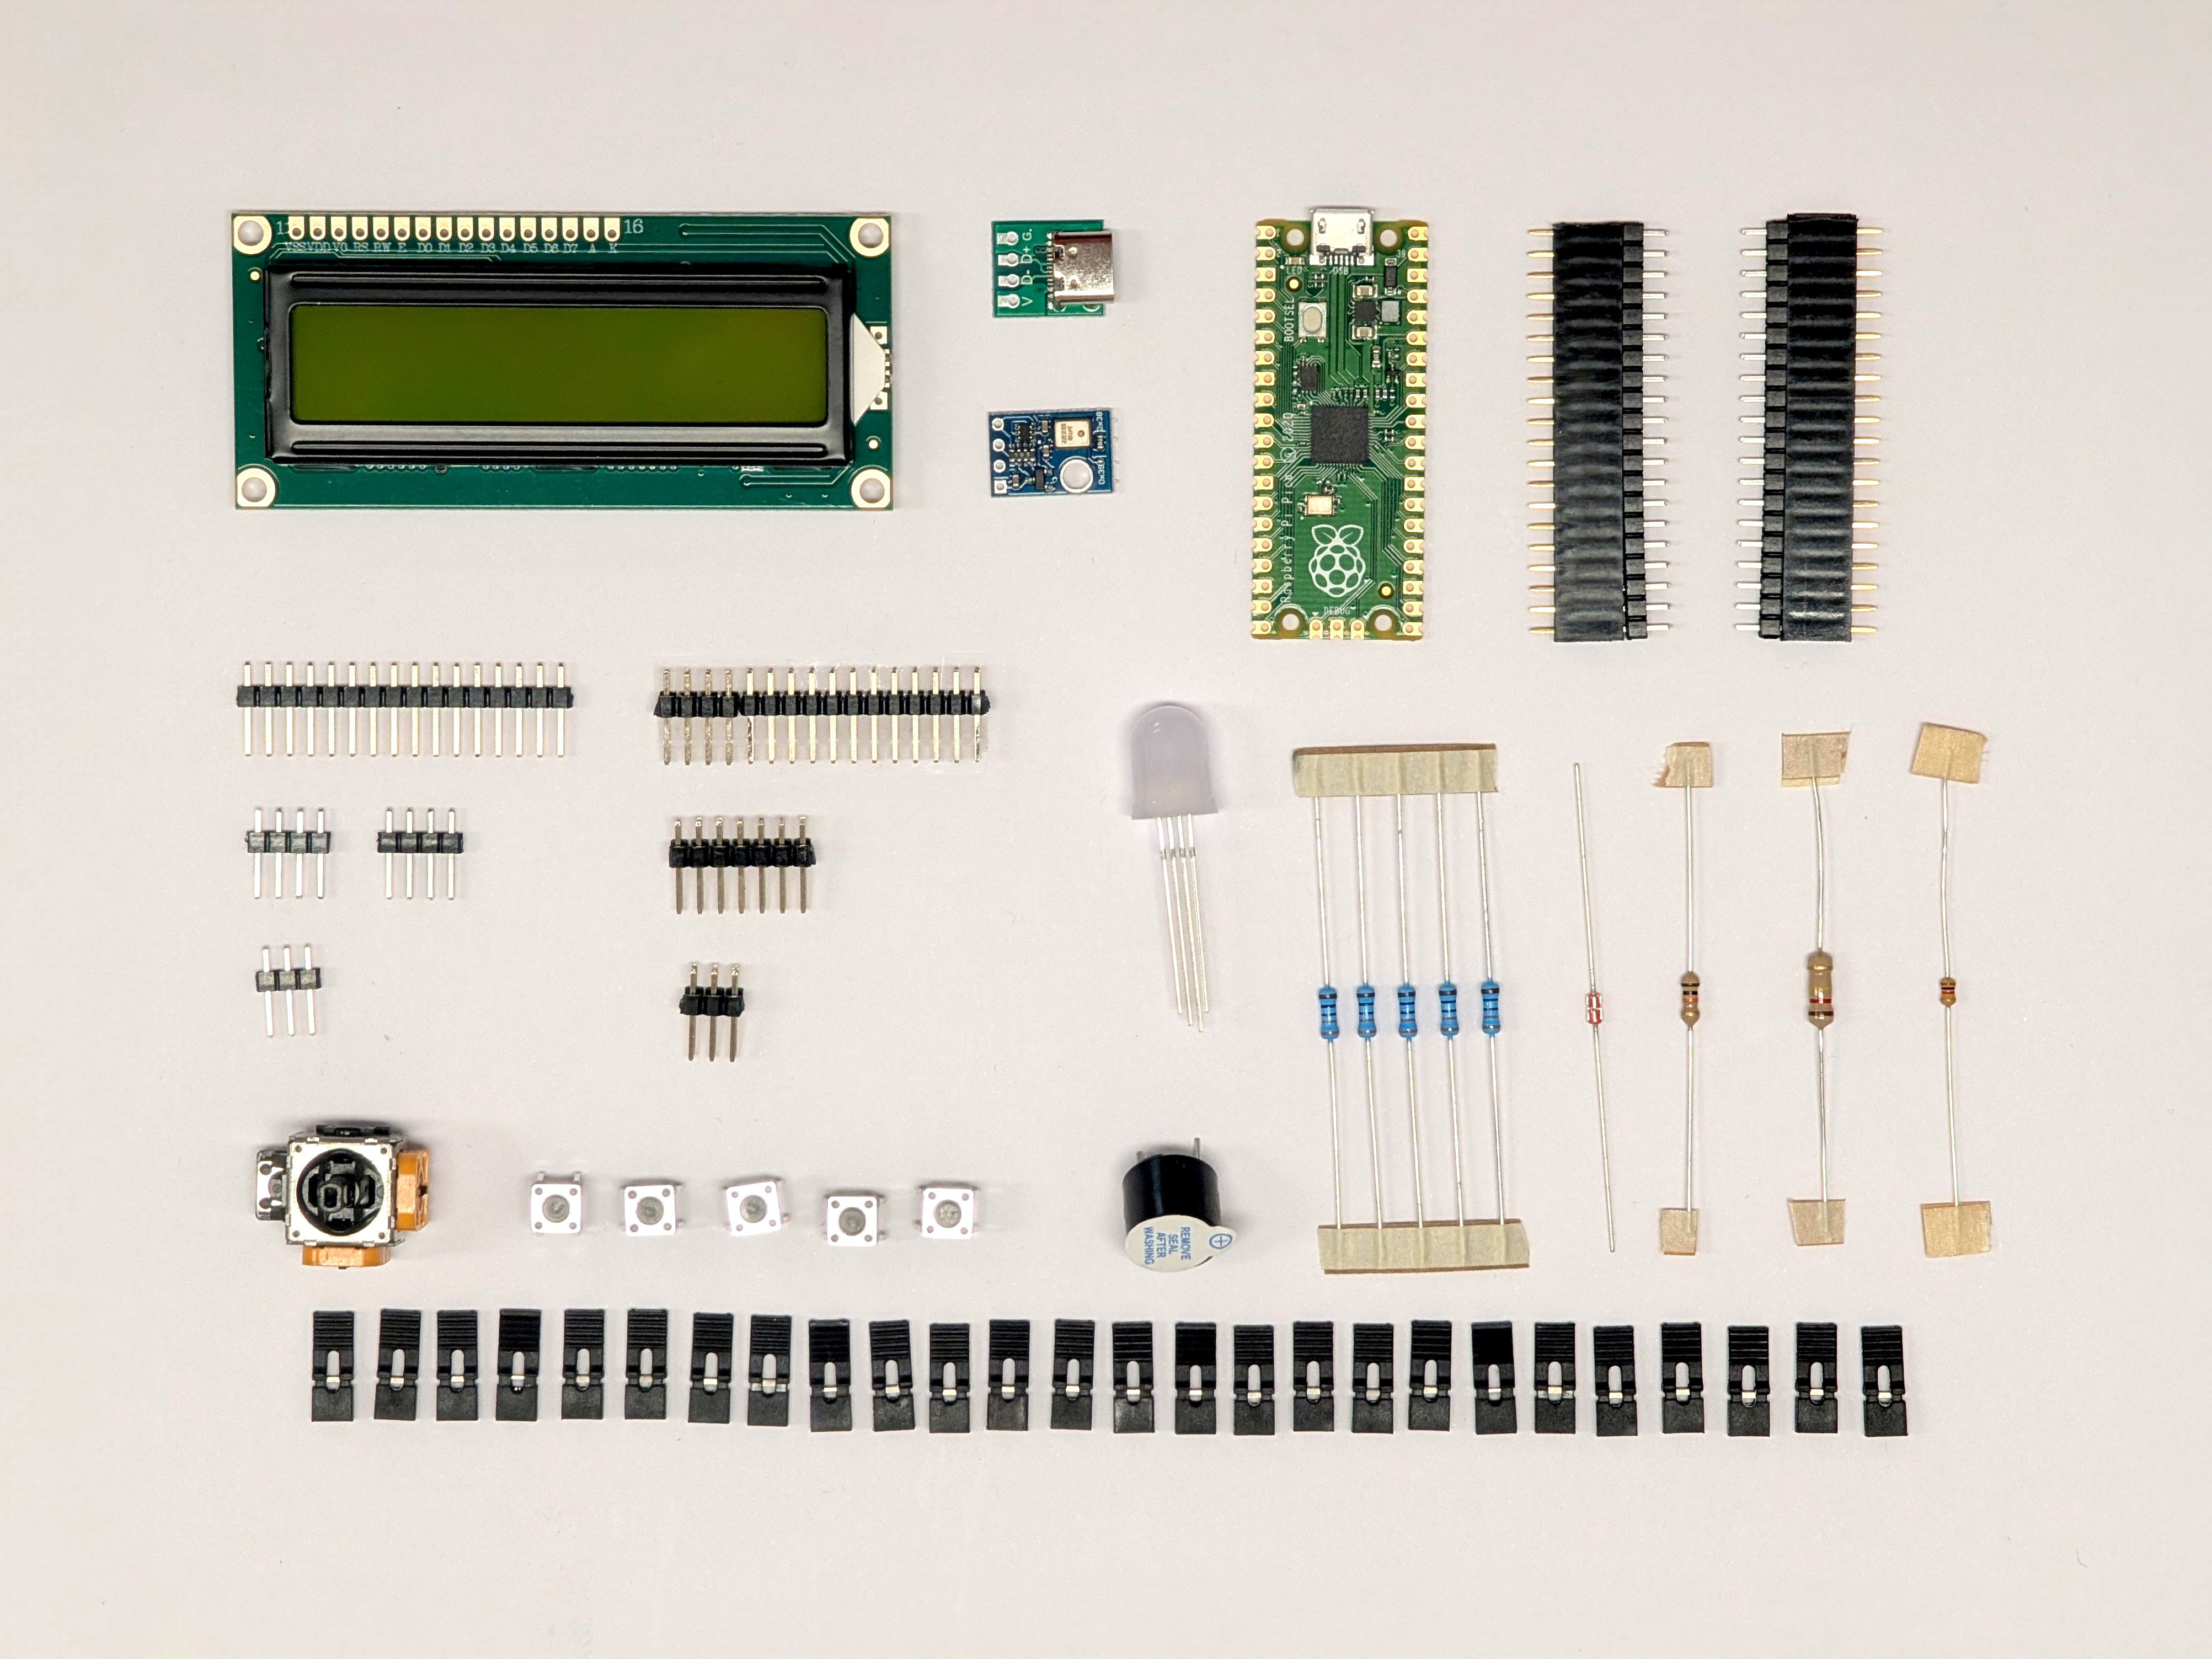
\includegraphics[width=0.8\textwidth]{overview_without_pcb.jpg}
\end{figure}

Prüfe zuerst, ob alle Teile da sind:

\begin{itemize}
    \item 1x Buzzerino-Platine
    \item 1x Raspberry Pi Pico
    \item 1x 1602A-LCD-Display
    \item 1x AHT10 Temperatur- und Luftfeuchtigkeitssensor
    \item 1x USB-C-Breakout-Board
    \item 1x 10 mm RGB-LED
    \item 1x Buzzer
    \item 1x analoger Joystick
    \item 5x Taster
    \item 1x 100-k$\Omega$-NTC
    \item 5x 330-$\Omega$-Widerstände
    \item 1x 1-k$\Omega$-Widerstand
    \item 1x 10-k$\Omega$-Widerstand
    \item 1x 120-k$\Omega$-Widerstand
    \item verschiedene Stiftleisten
    \item 26 Jumper
\end{itemize}

\section*{So lötest du richtig}

Wenn du zwei Teile verlöten willst:

\begin{enumerate}
    \item Stecke das Teil in die richtige Position.
    \item Drehe die Platine vorsichtig um.
    \item Halte den Lötkolben an den Pin und an die Lötstelle.
    \item Gib dann ein wenig Lötzinn dazu.
    \item Nimm zuerst das Lötzinn weg, dann den Lötkolben.
    \item Lass alles kurz abkühlen.
\end{enumerate}

\textbf{Tipp:}
\begin{itemize}
    \item Erst \textbf{einen Pin} löten.
    \item Dann schauen, ob das Teil gerade sitzt.
    \item Danach die restlichen Pins löten.
\end{itemize}

\section*{Schritt-für-Schritt-Aufbau}

\subsection*{1. Raspberry Pi Pico vorbereiten}

Zuerst werden die beiden langen Stiftleisten an den Raspberry Pi Pico gelötet.

\textbf{Wichtig:}
\begin{itemize}
    \item Die Stiftleisten bestehen aus zwei zusammengesteckten Teilen.
    \item \textbf{Lass sie zusammengesteckt.}
    \item So bleiben die Pins gerade.
\end{itemize}

\begin{figure}[H]
    \centering
    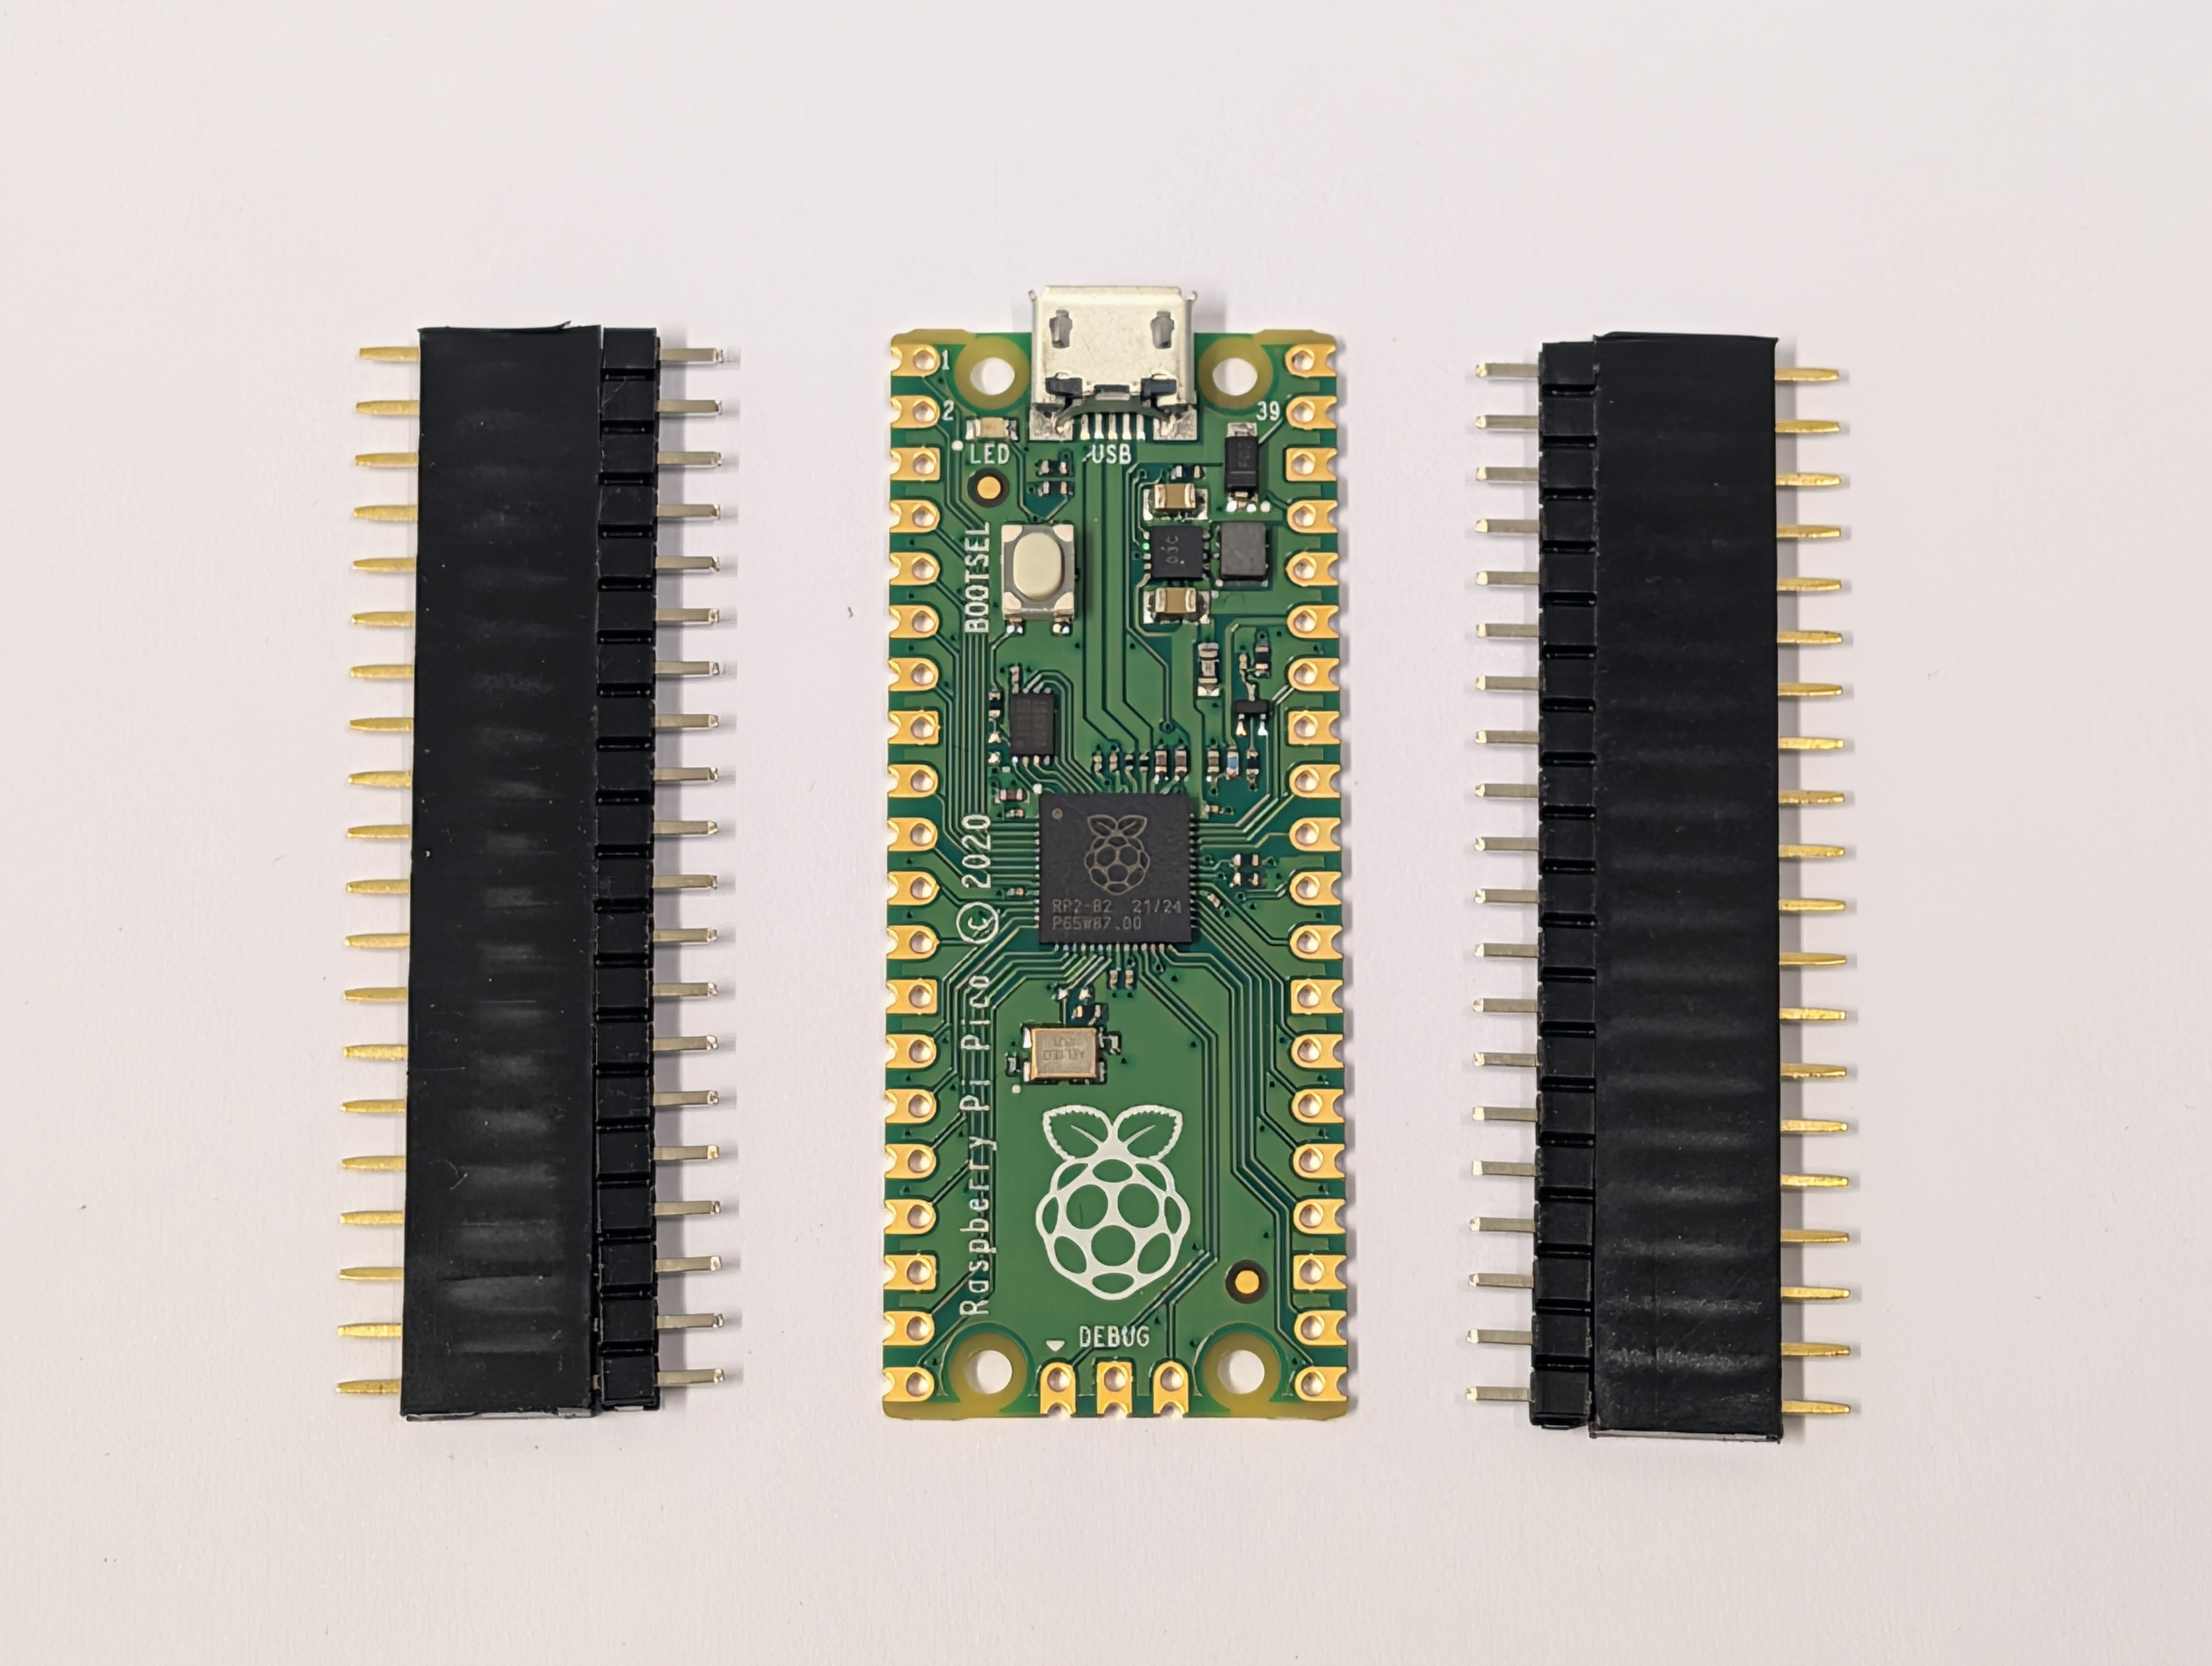
\includegraphics[width=0.75\textwidth]{pictures_of_construction/instruction_step_1.jpg}
\end{figure}

So geht’s:
\begin{enumerate}
    \item Stecke die beiden Stiftleisten in den Raspberry Pi Pico.
    \item Stecke das Ganze zusätzlich in die Buzzerino-Platine, damit alles gerade ausgerichtet ist.
    \item Löte zuerst die \textbf{vier Eckpins}.
    \item Prüfe, ob alles gerade sitzt.
    \item Ziehe den Raspberry Pi Pico wieder heraus.
    \item Löte jetzt alle übrigen Pins fest.
\end{enumerate}

\begin{figure}[H]
    \centering
    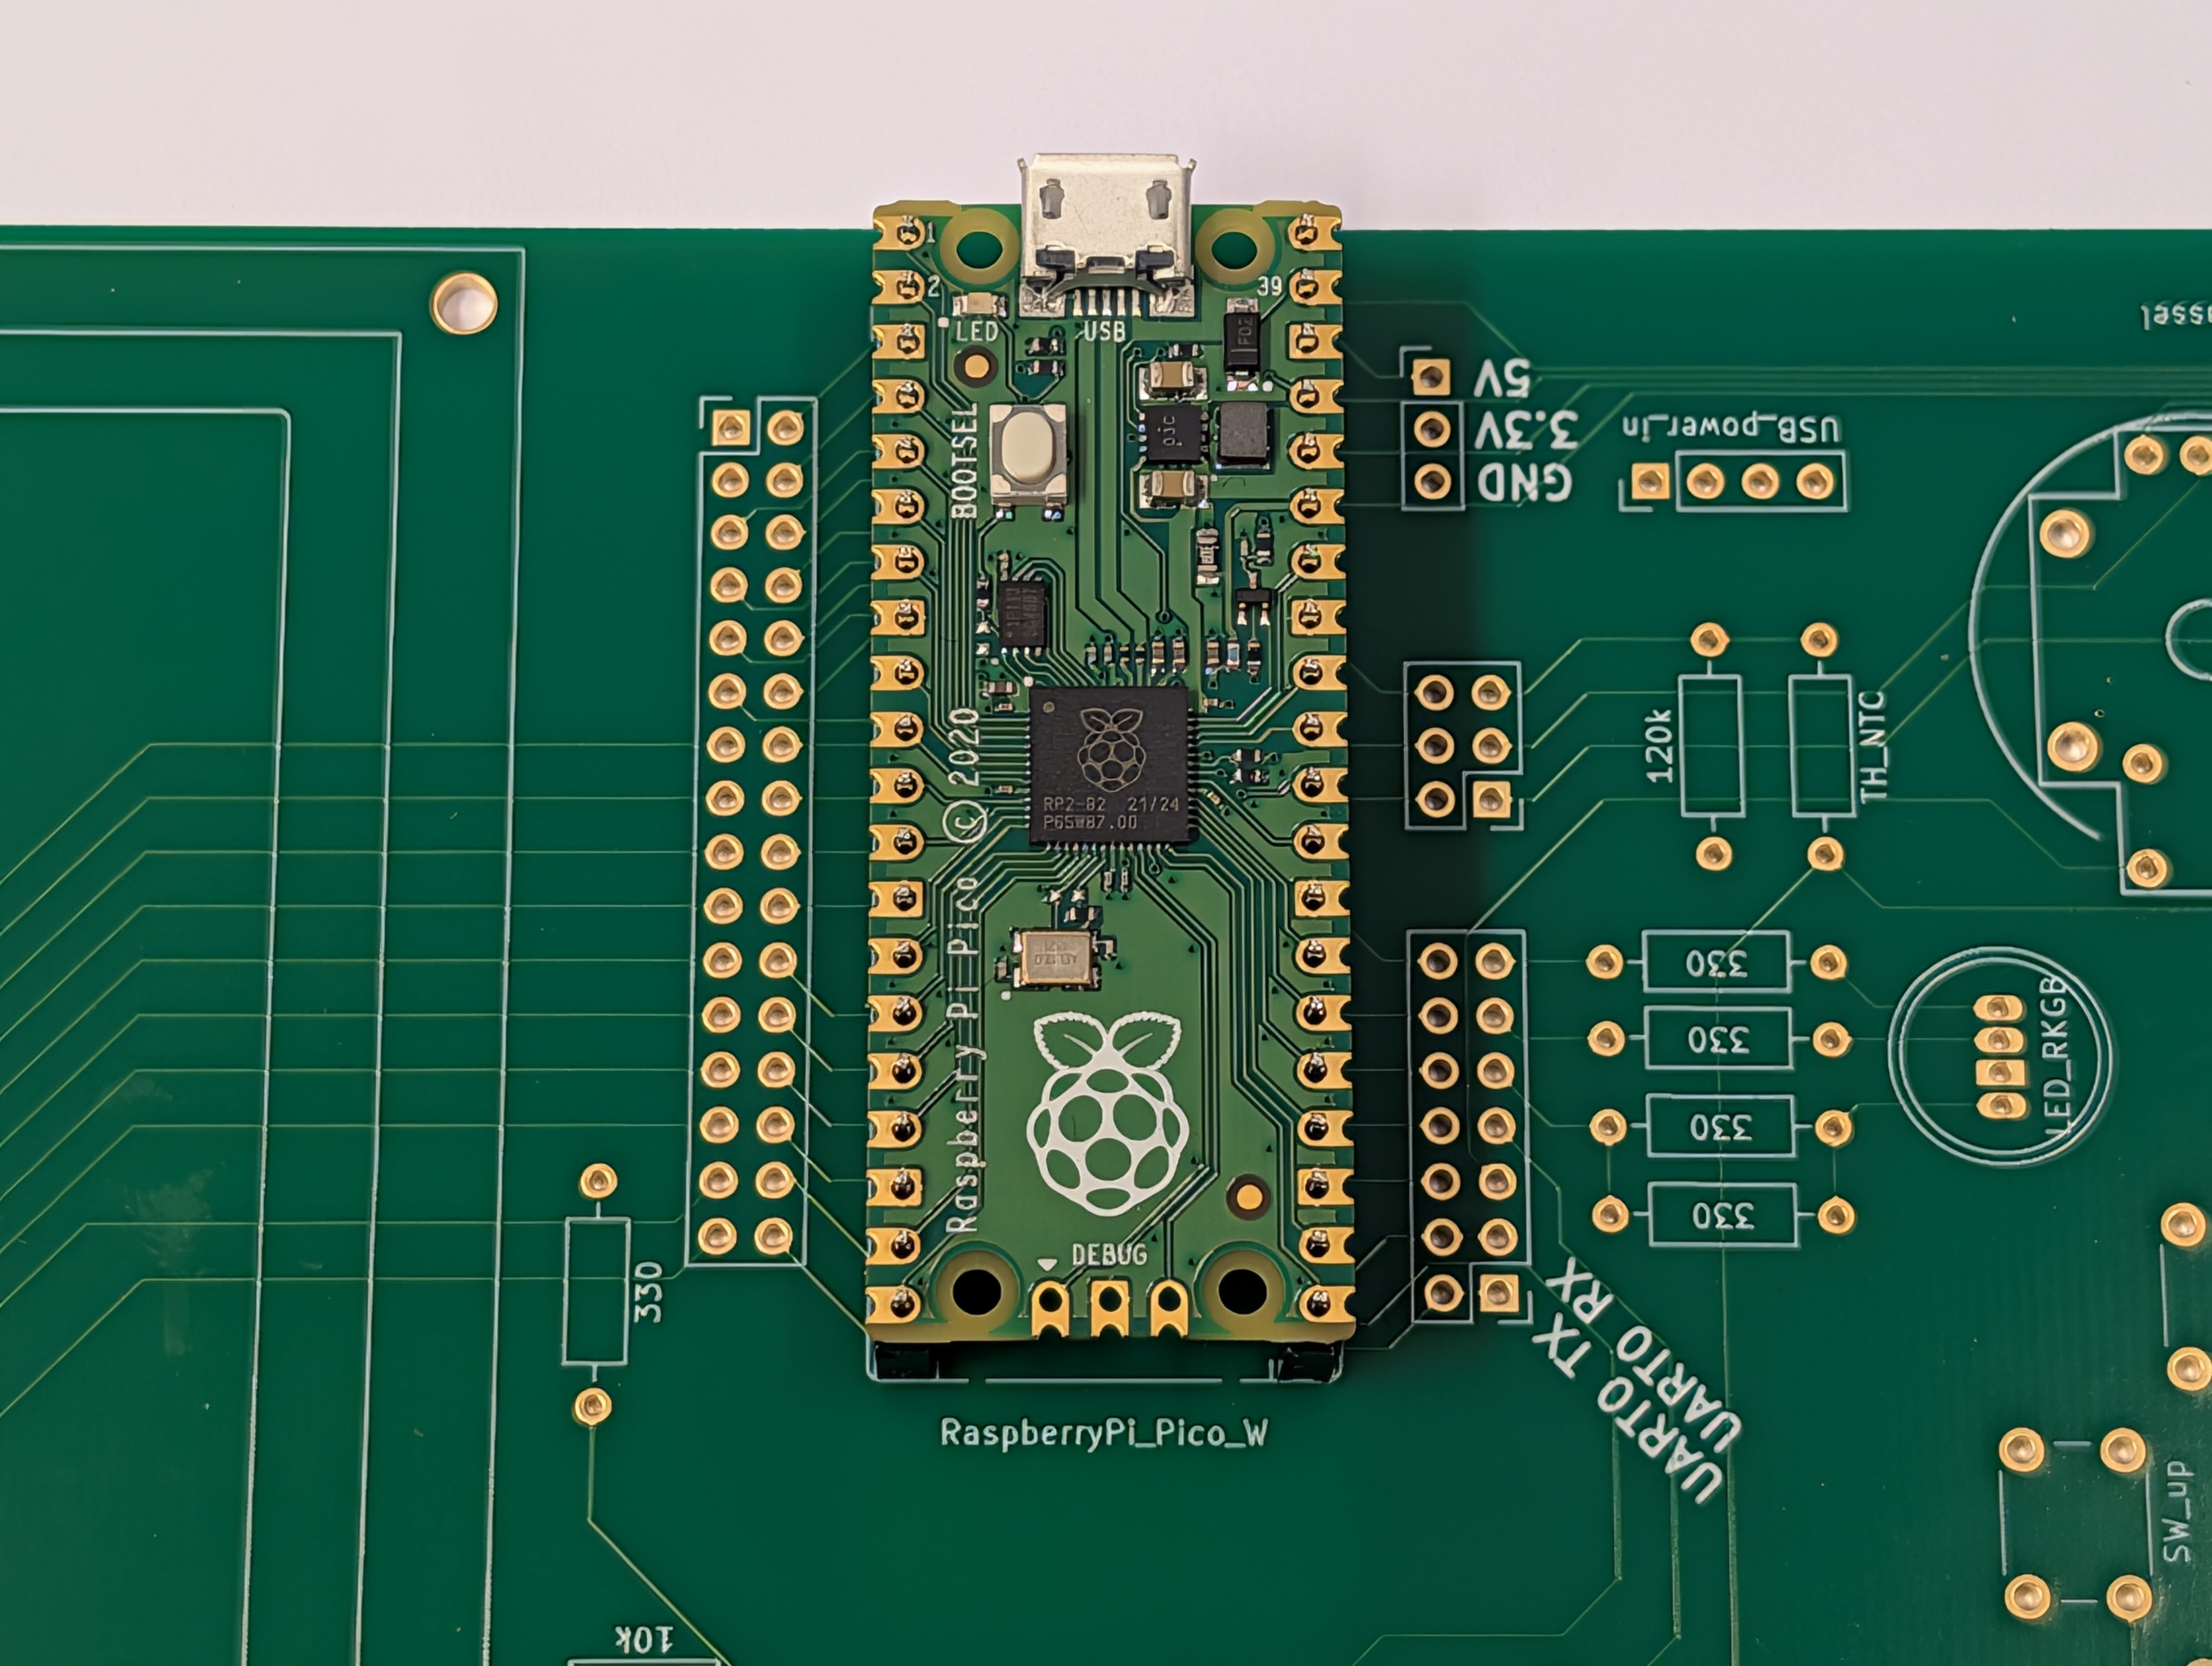
\includegraphics[width=0.75\textwidth]{pictures_of_construction/instruction_step_2.jpg}
\end{figure}

\begin{figure}[H]
    \centering
    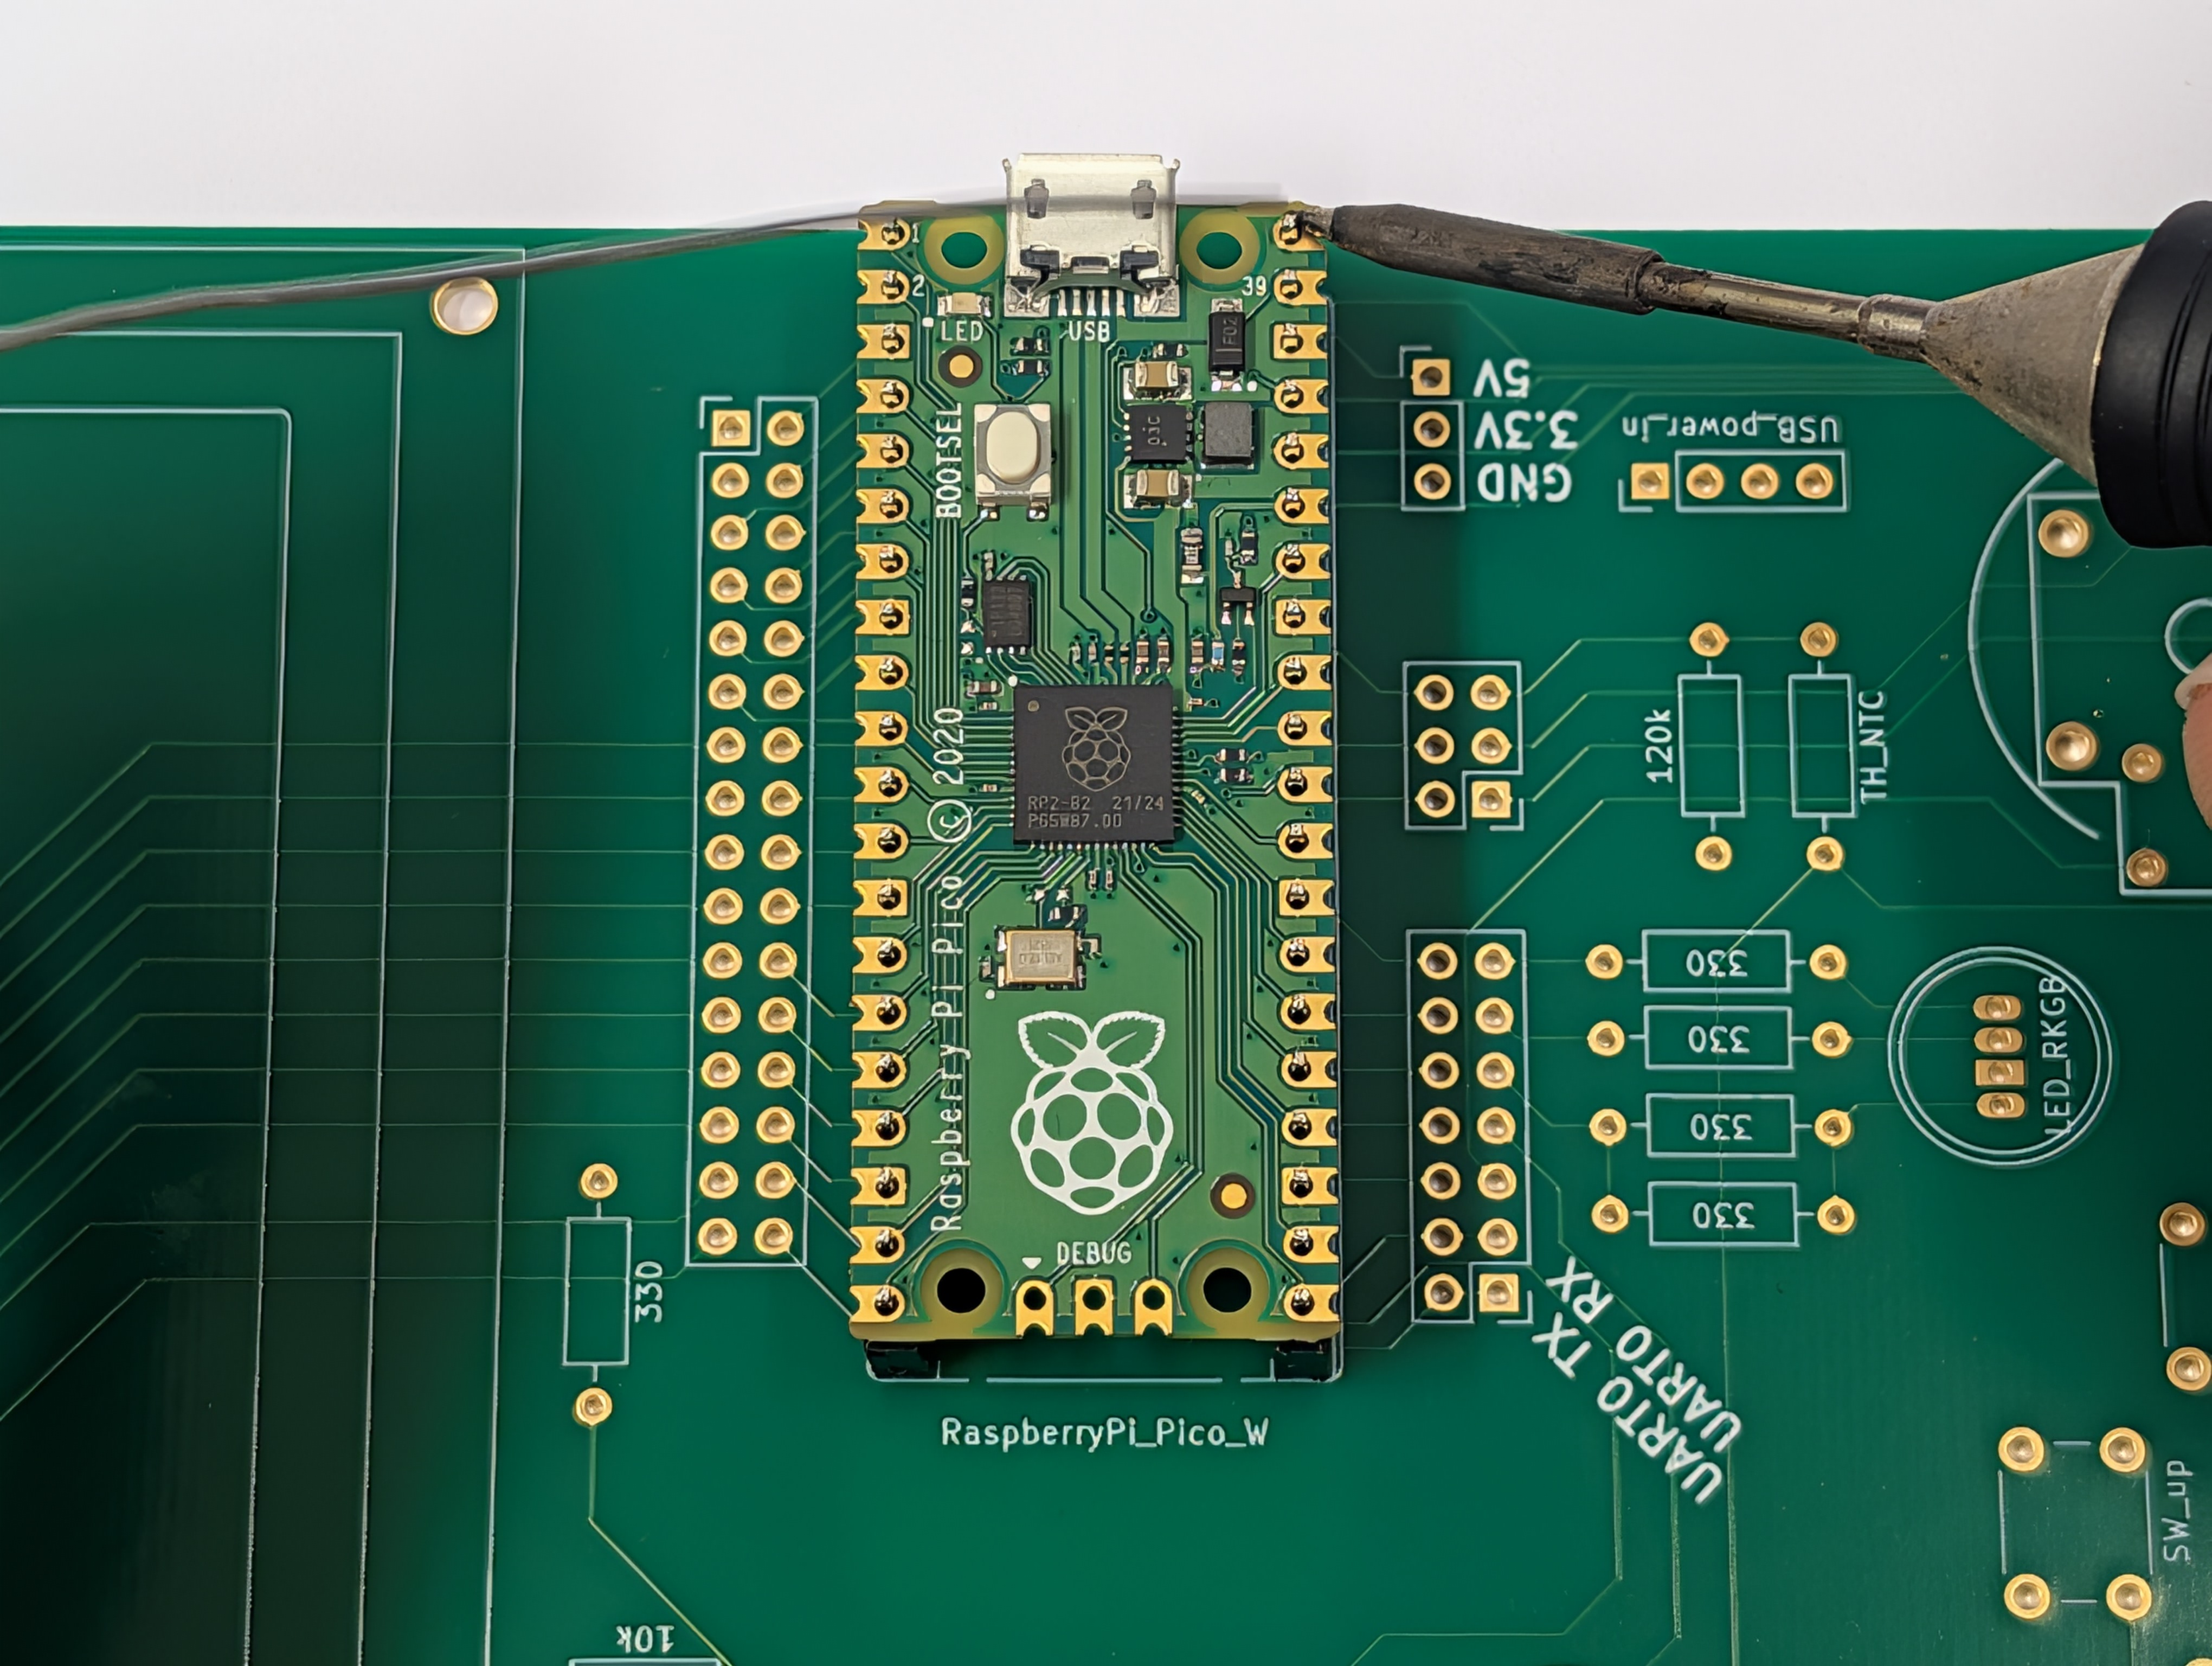
\includegraphics[width=0.75\textwidth]{pictures_of_construction/instruction_step_3.jpg}
\end{figure}

\begin{figure}[H]
    \centering
    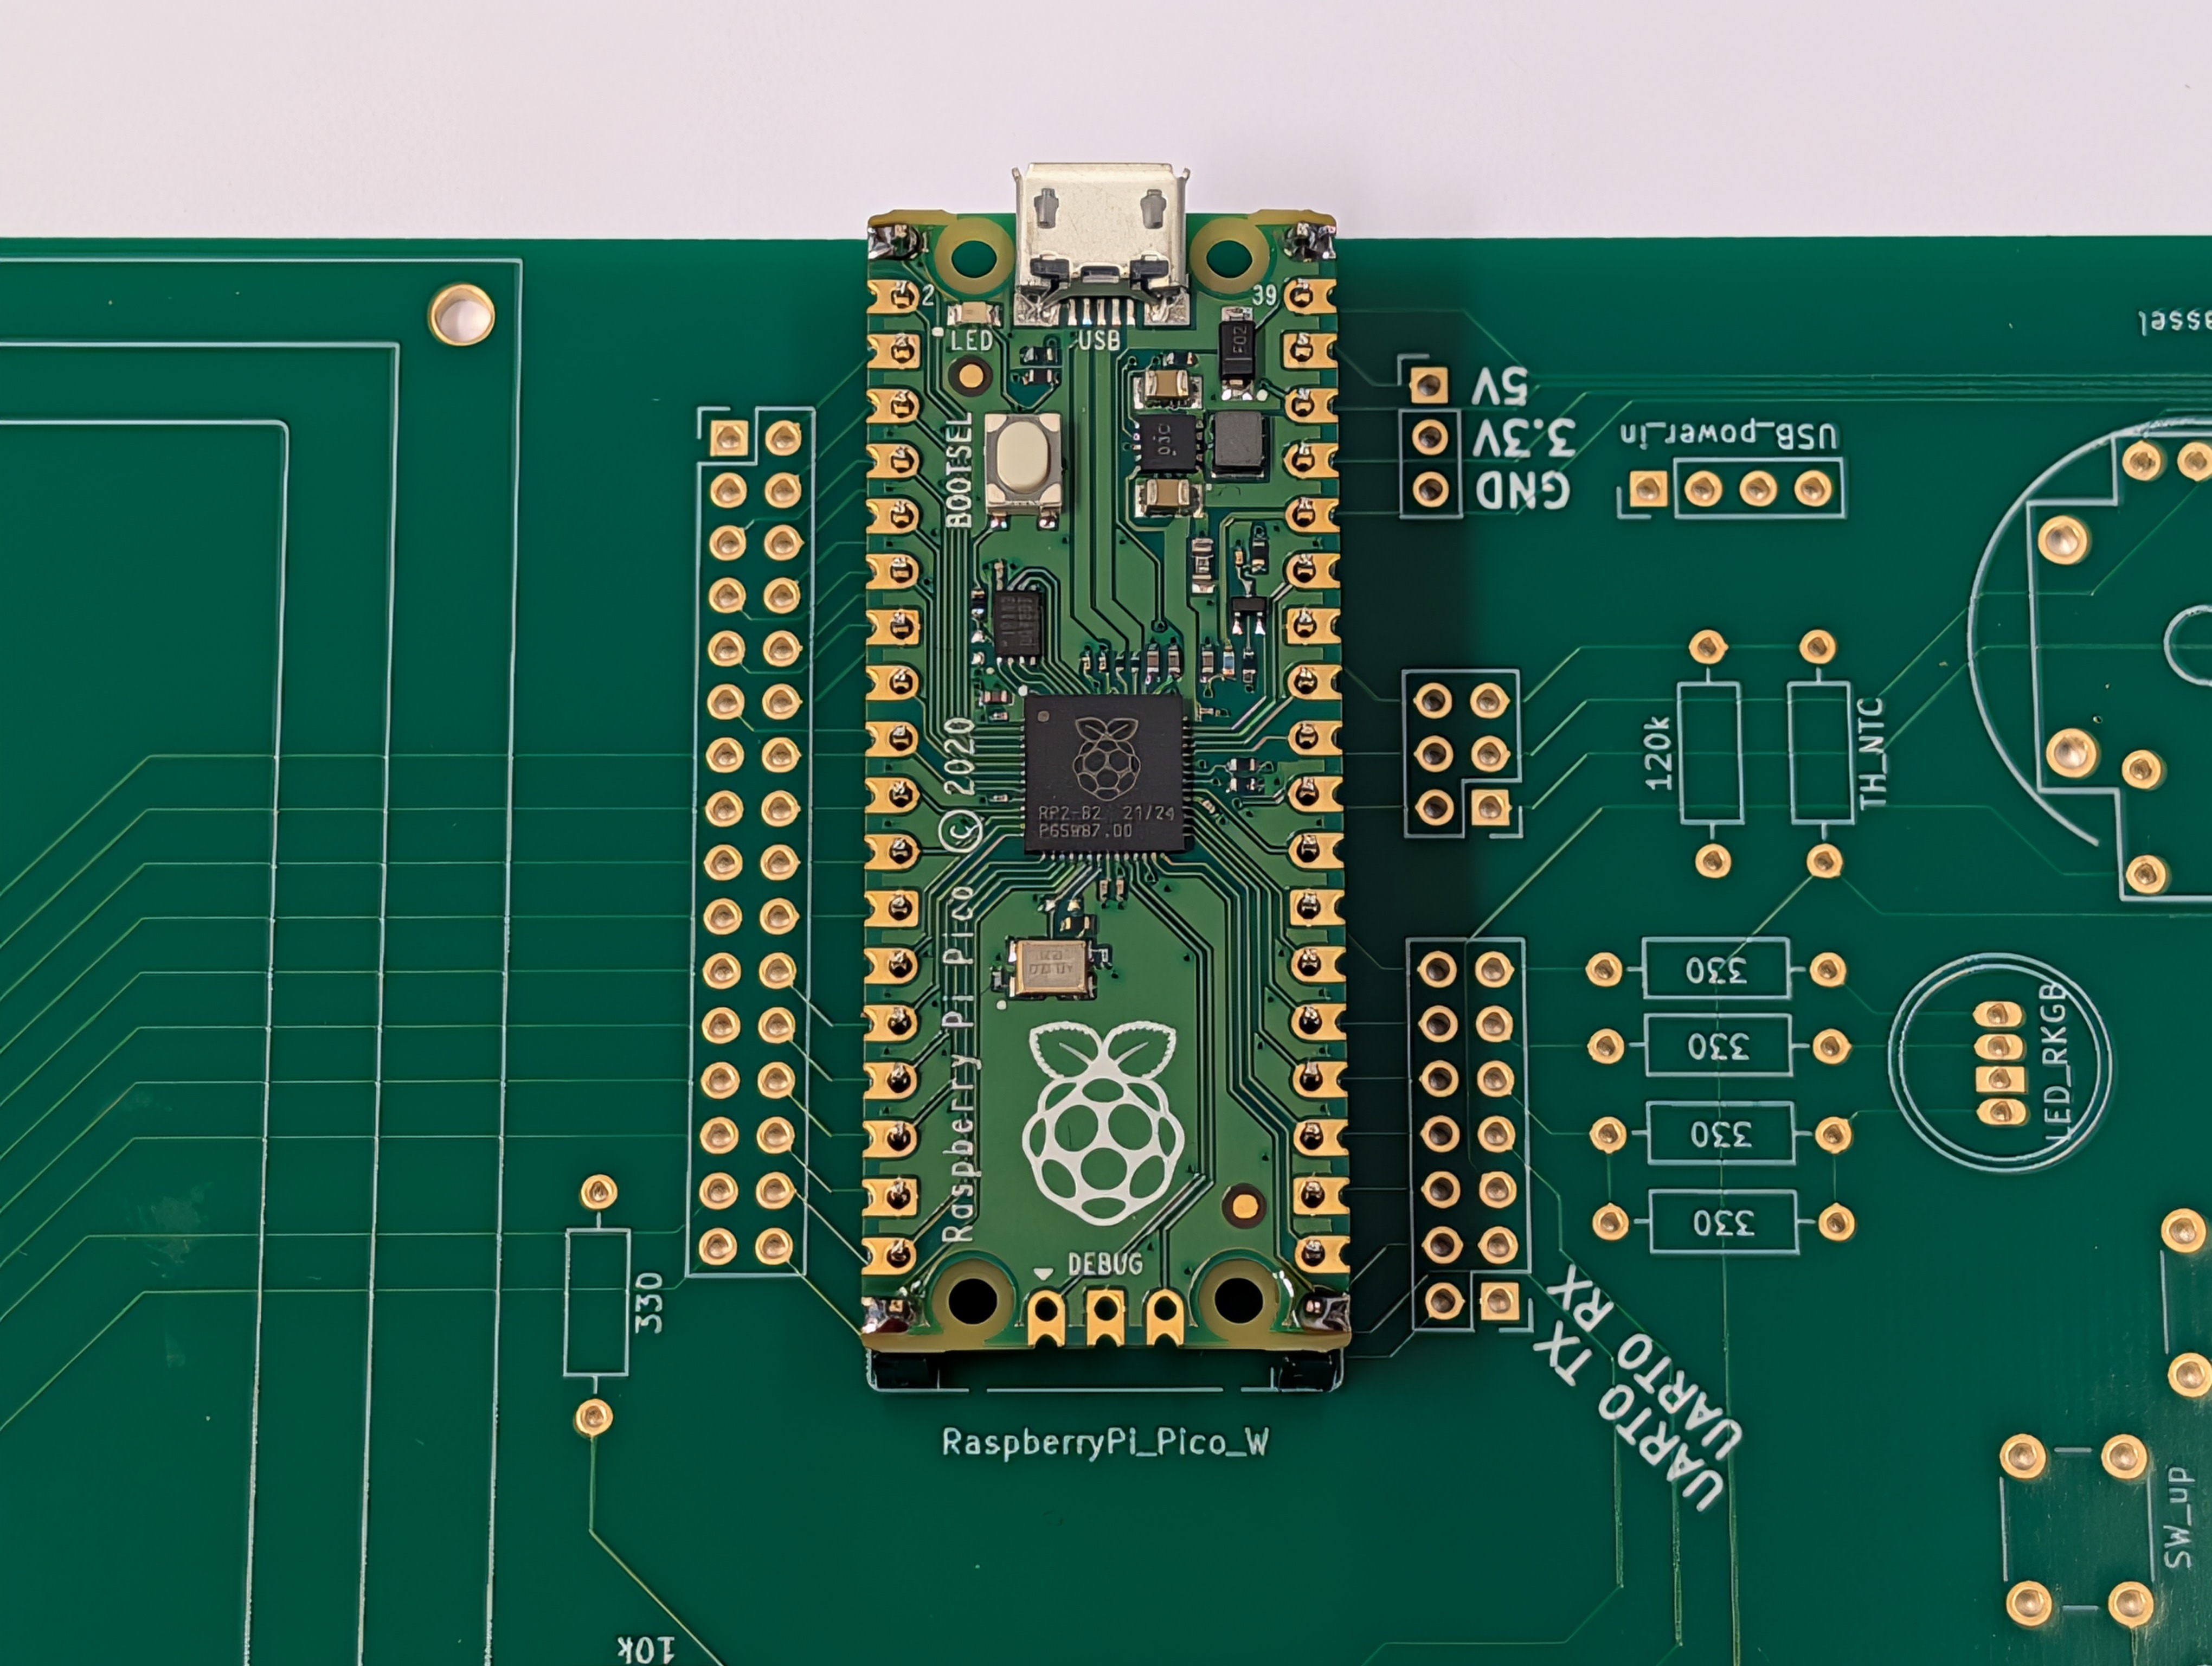
\includegraphics[width=0.75\textwidth]{pictures_of_construction/instruction_step_4.jpg}
\end{figure}

\begin{figure}[H]
    \centering
    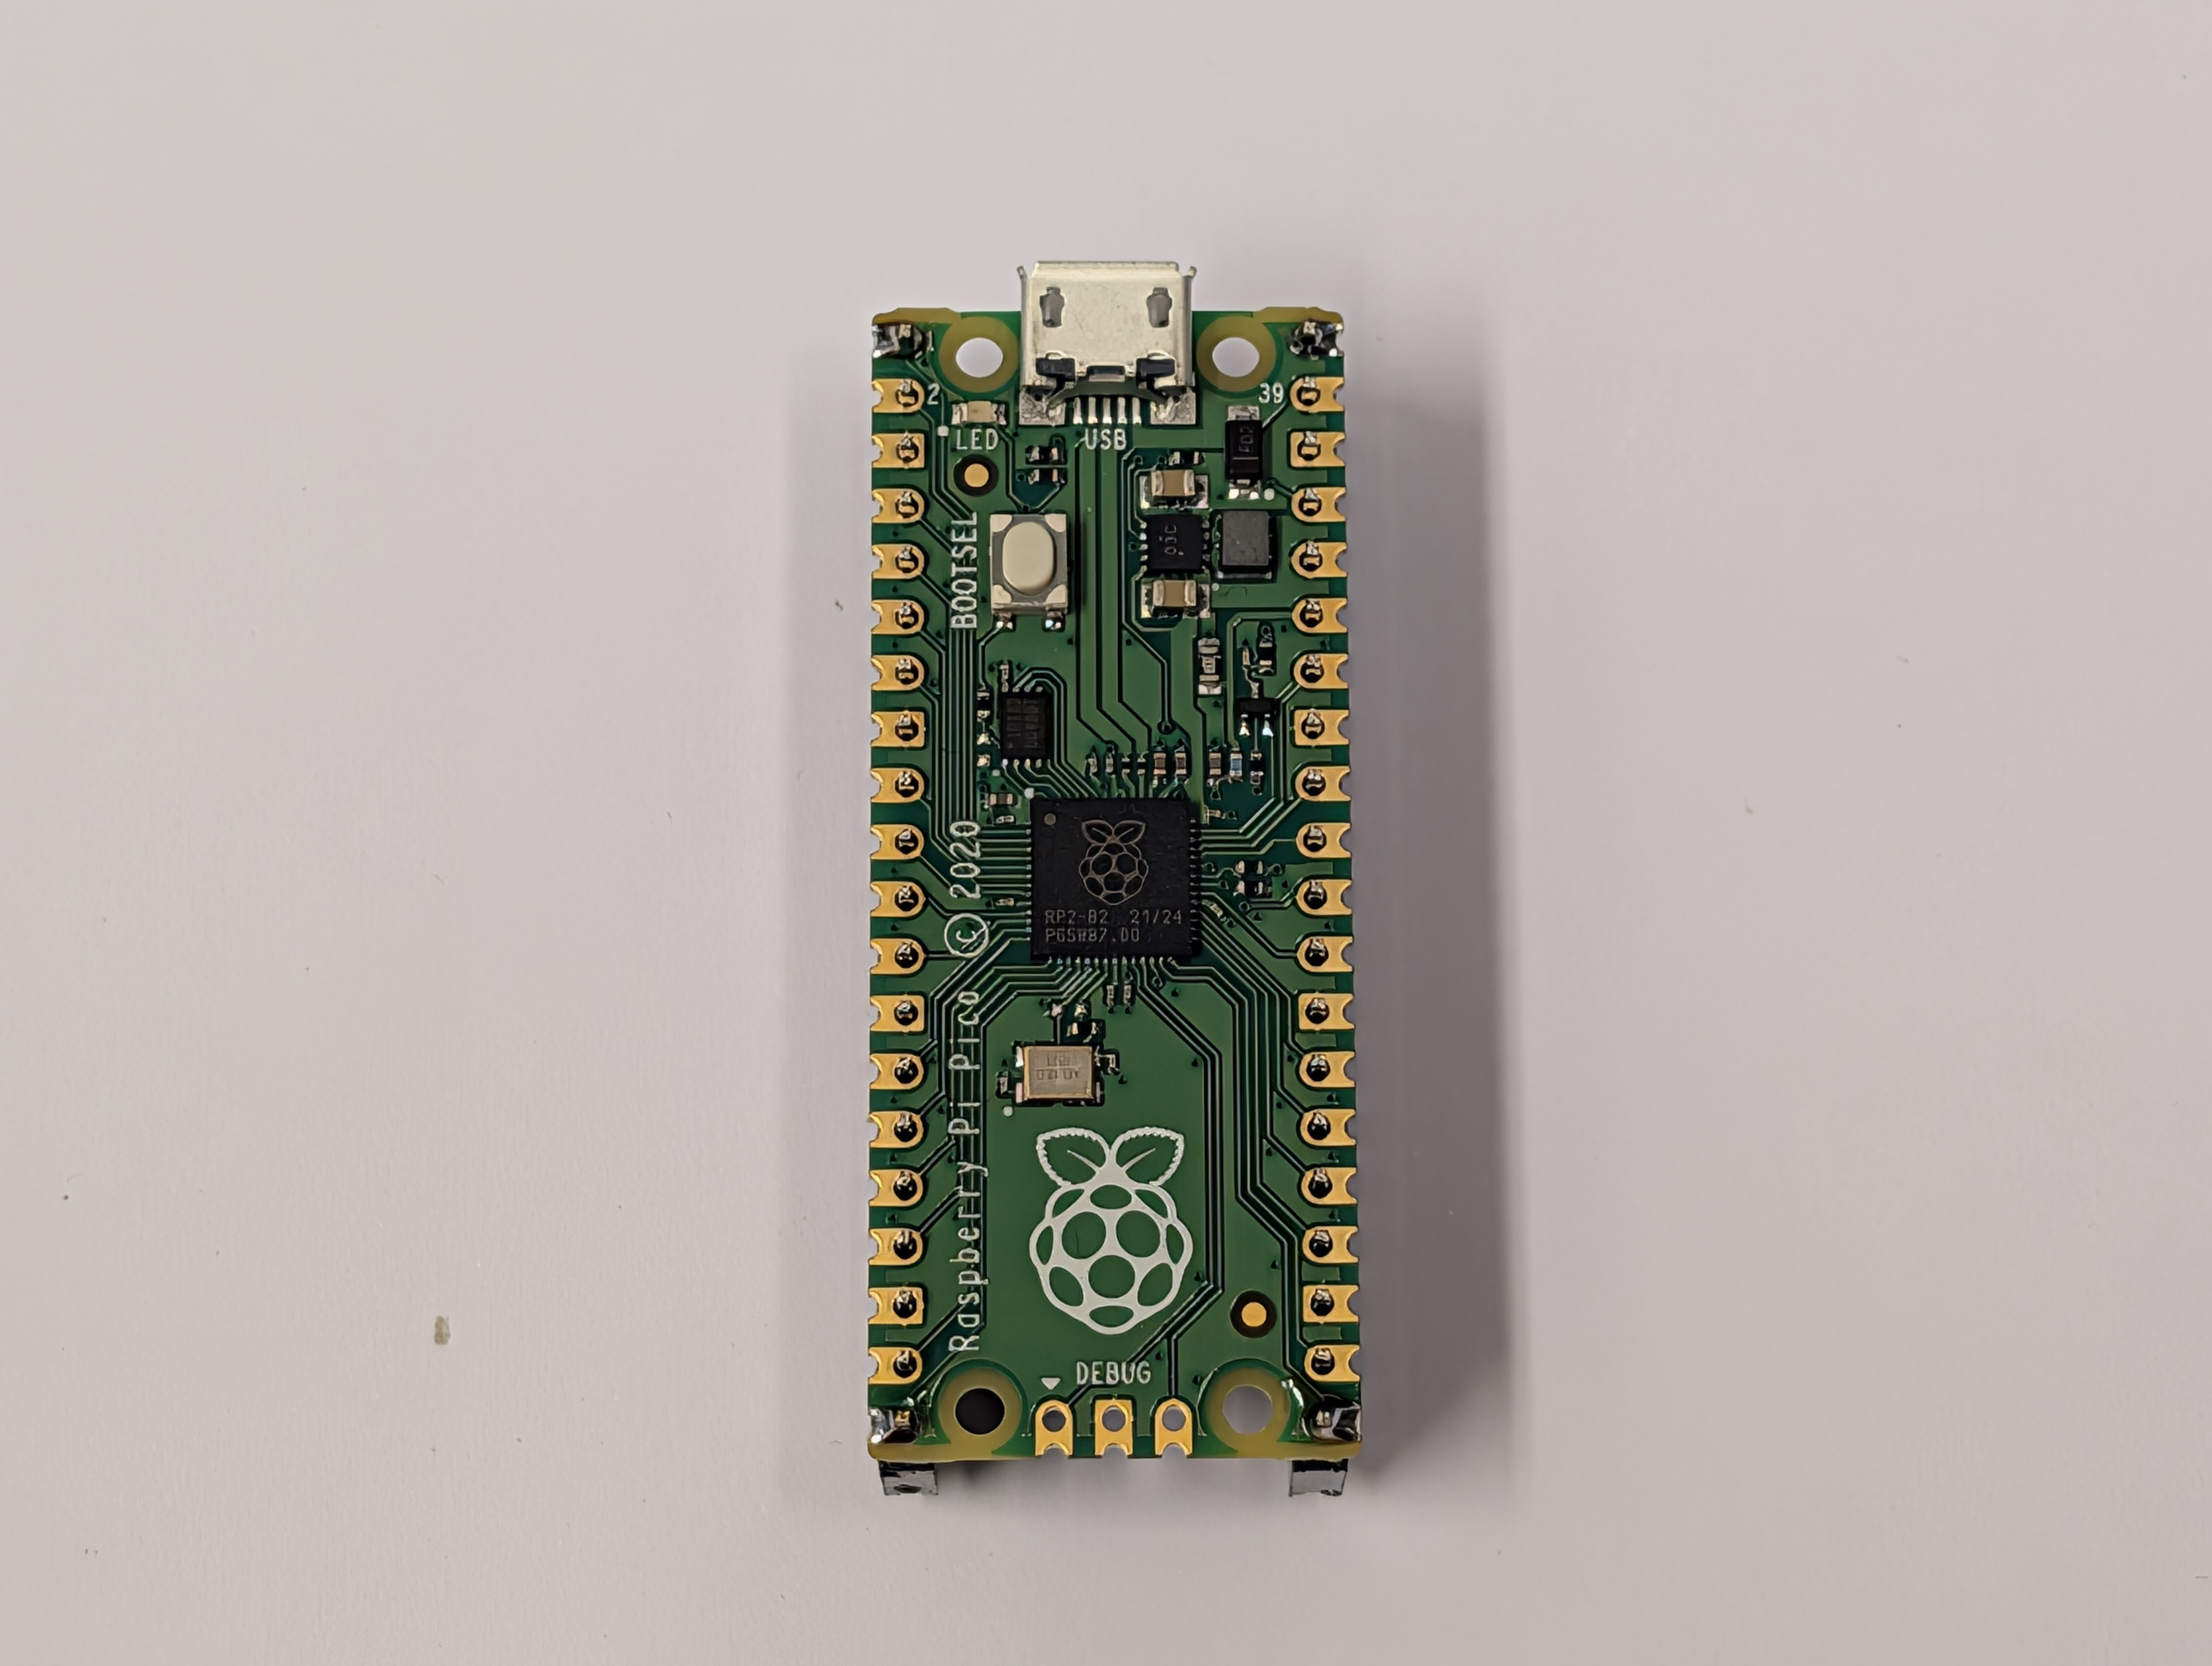
\includegraphics[width=0.75\textwidth]{pictures_of_construction/instruction_step_5.jpg}
\end{figure}

\begin{figure}[H]
    \centering
    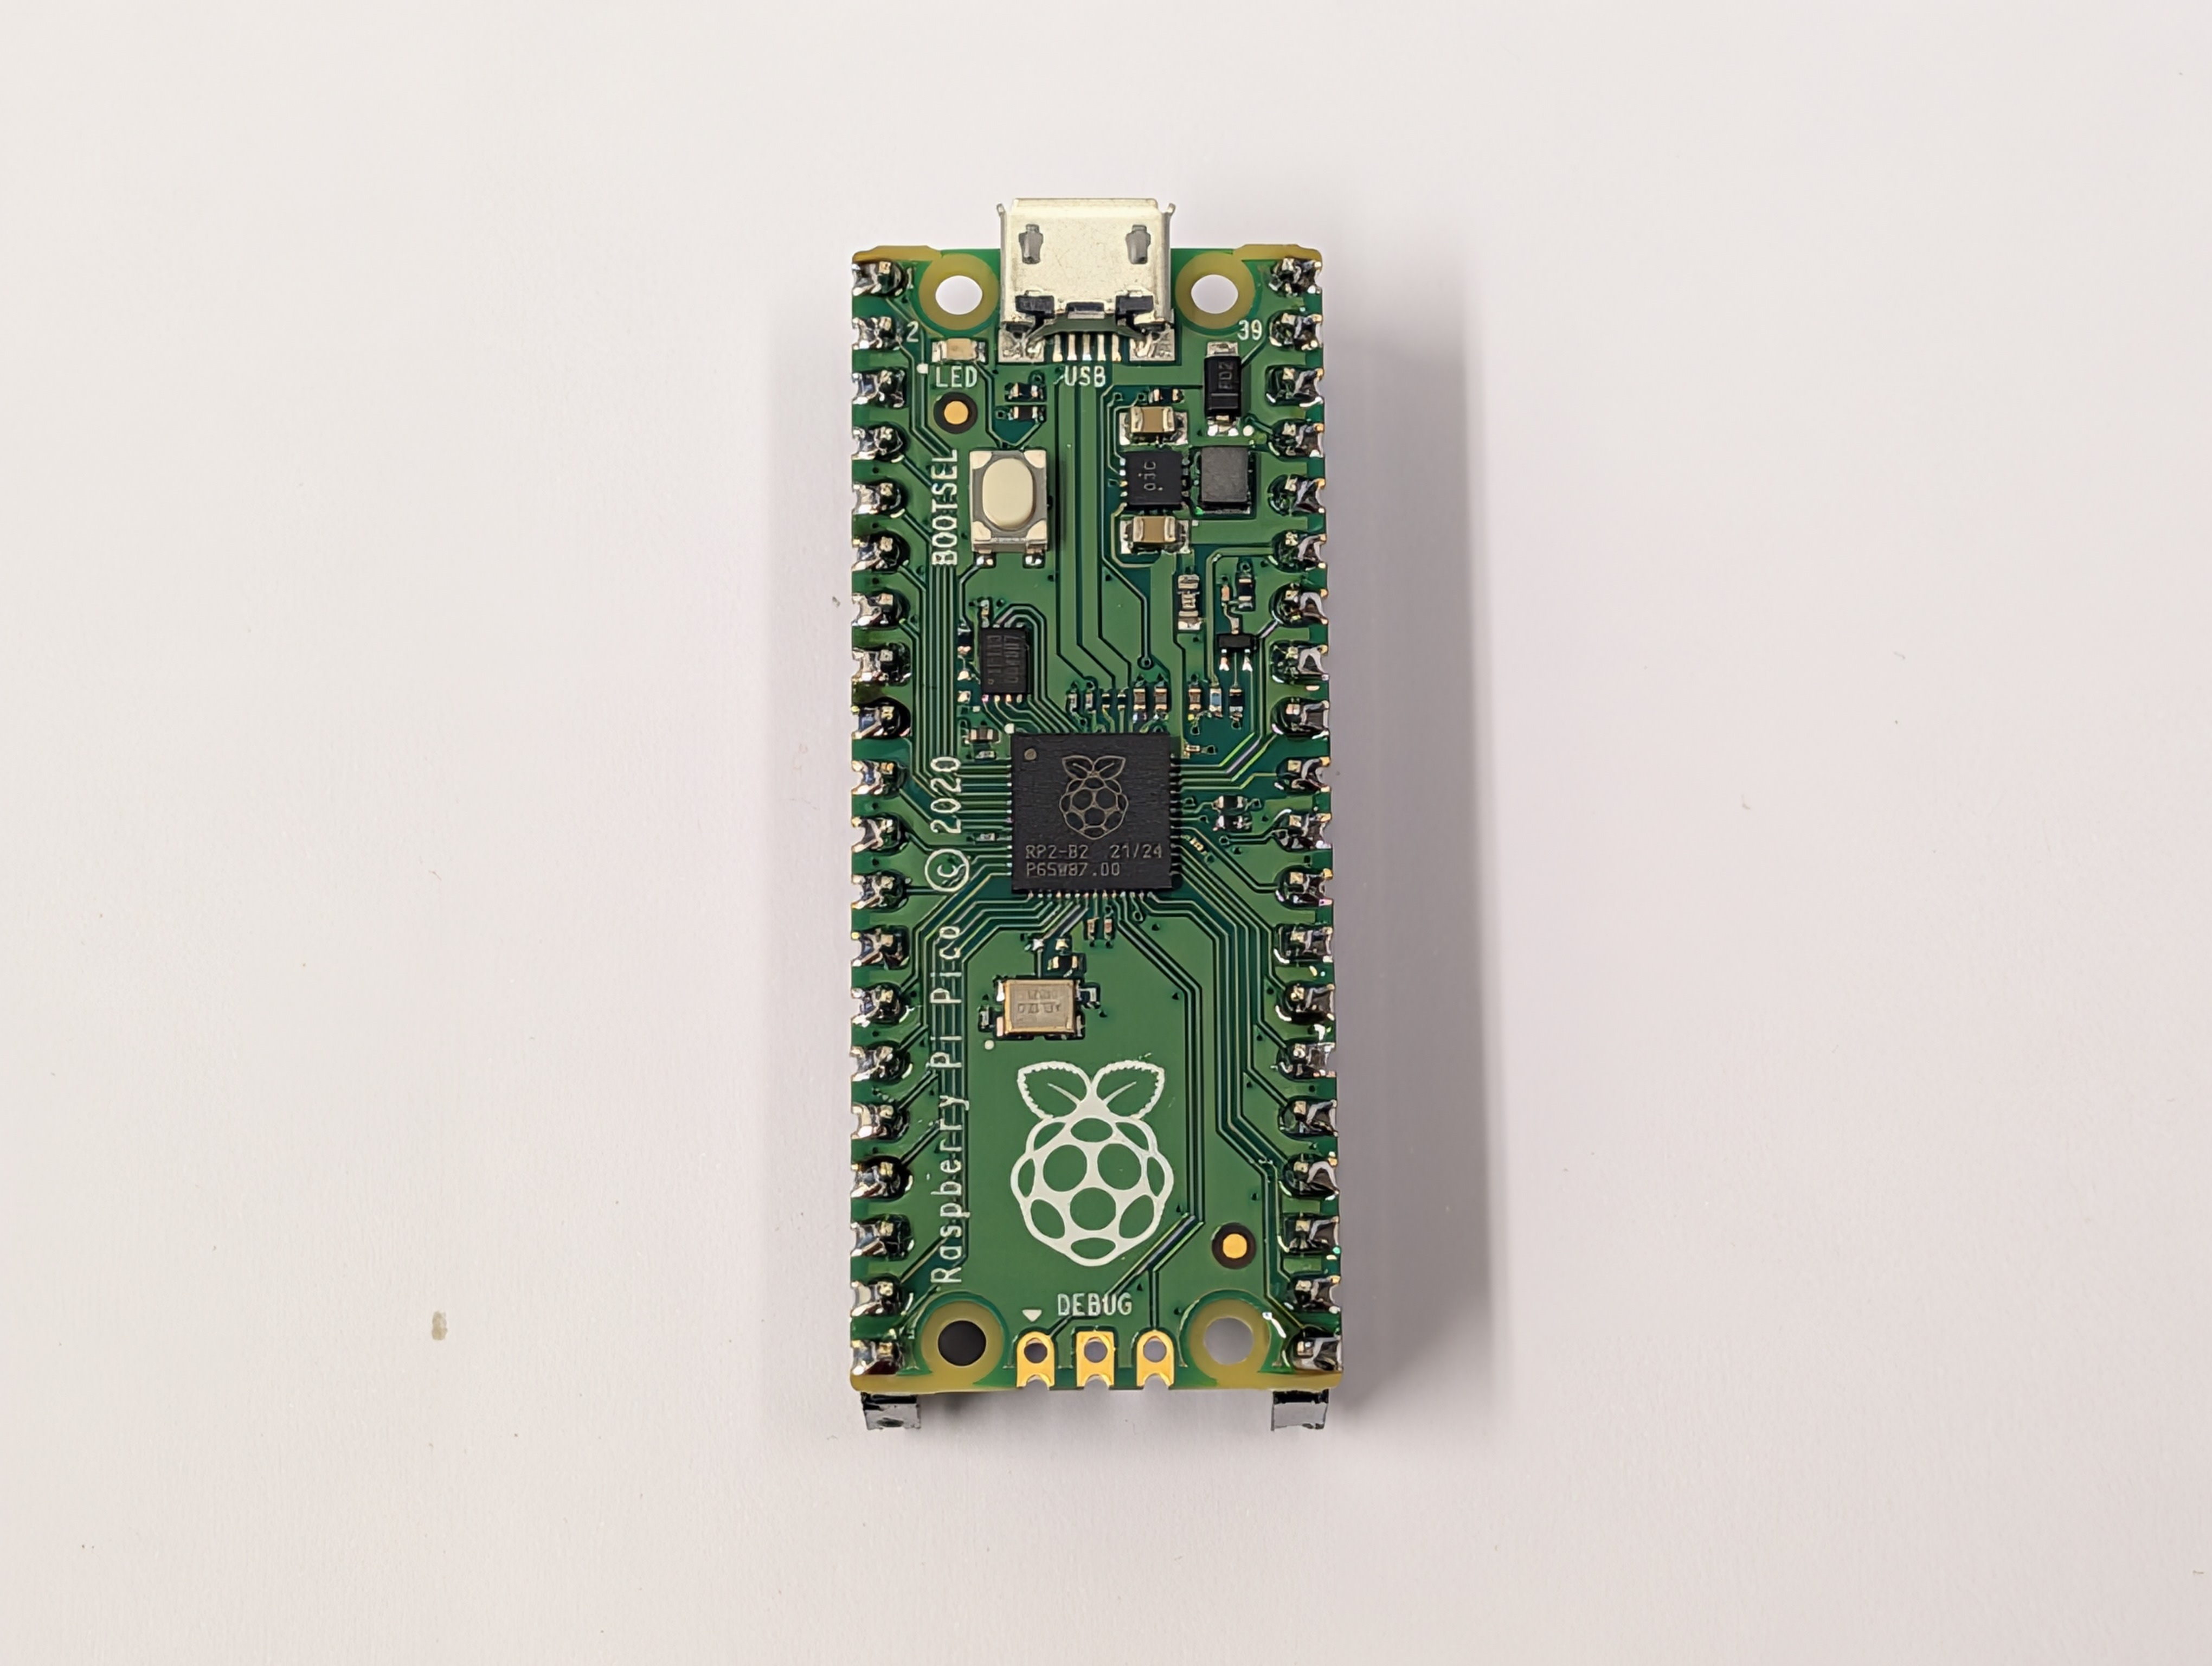
\includegraphics[width=0.75\textwidth]{pictures_of_construction/instruction_step_6.jpg}
\end{figure}

\subsection*{2. USB-C-Breakout-Board vorbereiten}

Jetzt bekommt das USB-C-Breakout-Board eine kleine Stiftleiste.

\begin{figure}[H]
    \centering
    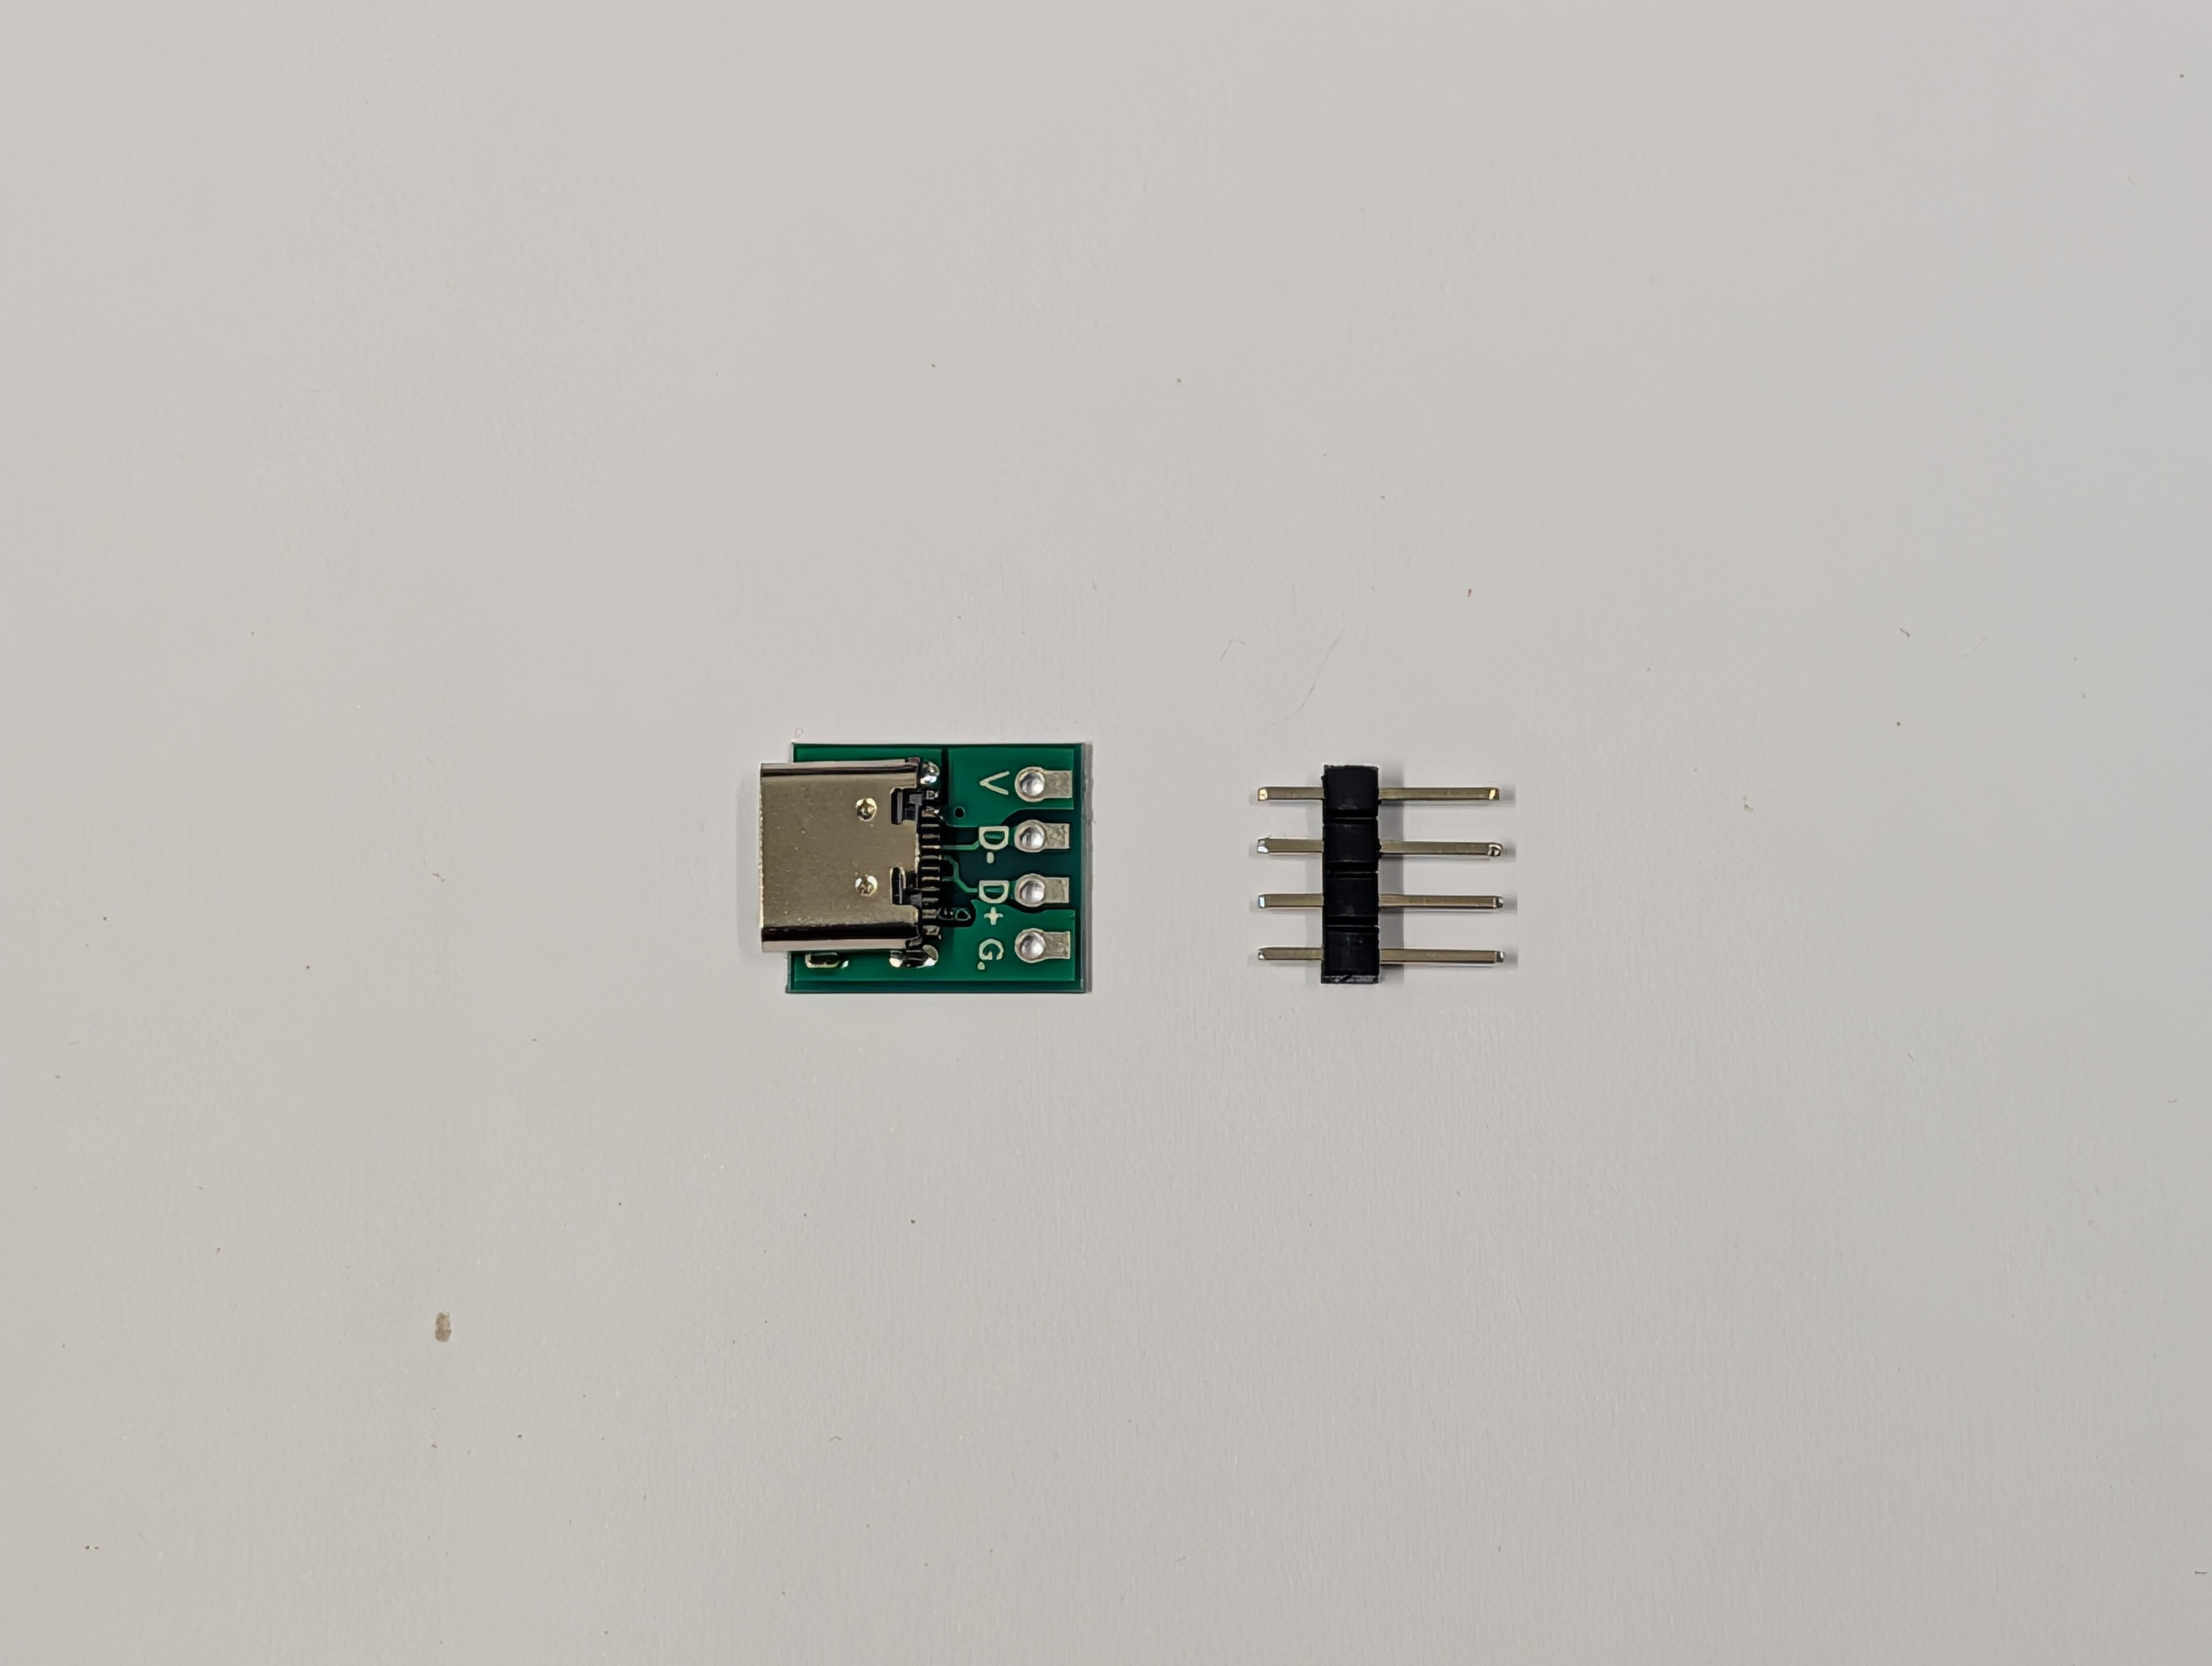
\includegraphics[width=0.75\textwidth]{pictures_of_construction/instruction_step_7.jpg}
\end{figure}

So geht’s:
\begin{enumerate}
    \item Stecke die 1x4-Stiftleiste in das Board.
    \item Löte zuerst nur \textbf{einen Pin}.
    \item Prüfe, ob die Stiftleiste gerade steht.
    \item Falls sie schief ist: Lötstelle nochmal kurz erhitzen und gerade richten.
    \item Löte dann alle Pins fest.
\end{enumerate}

\begin{figure}[H]
    \centering
    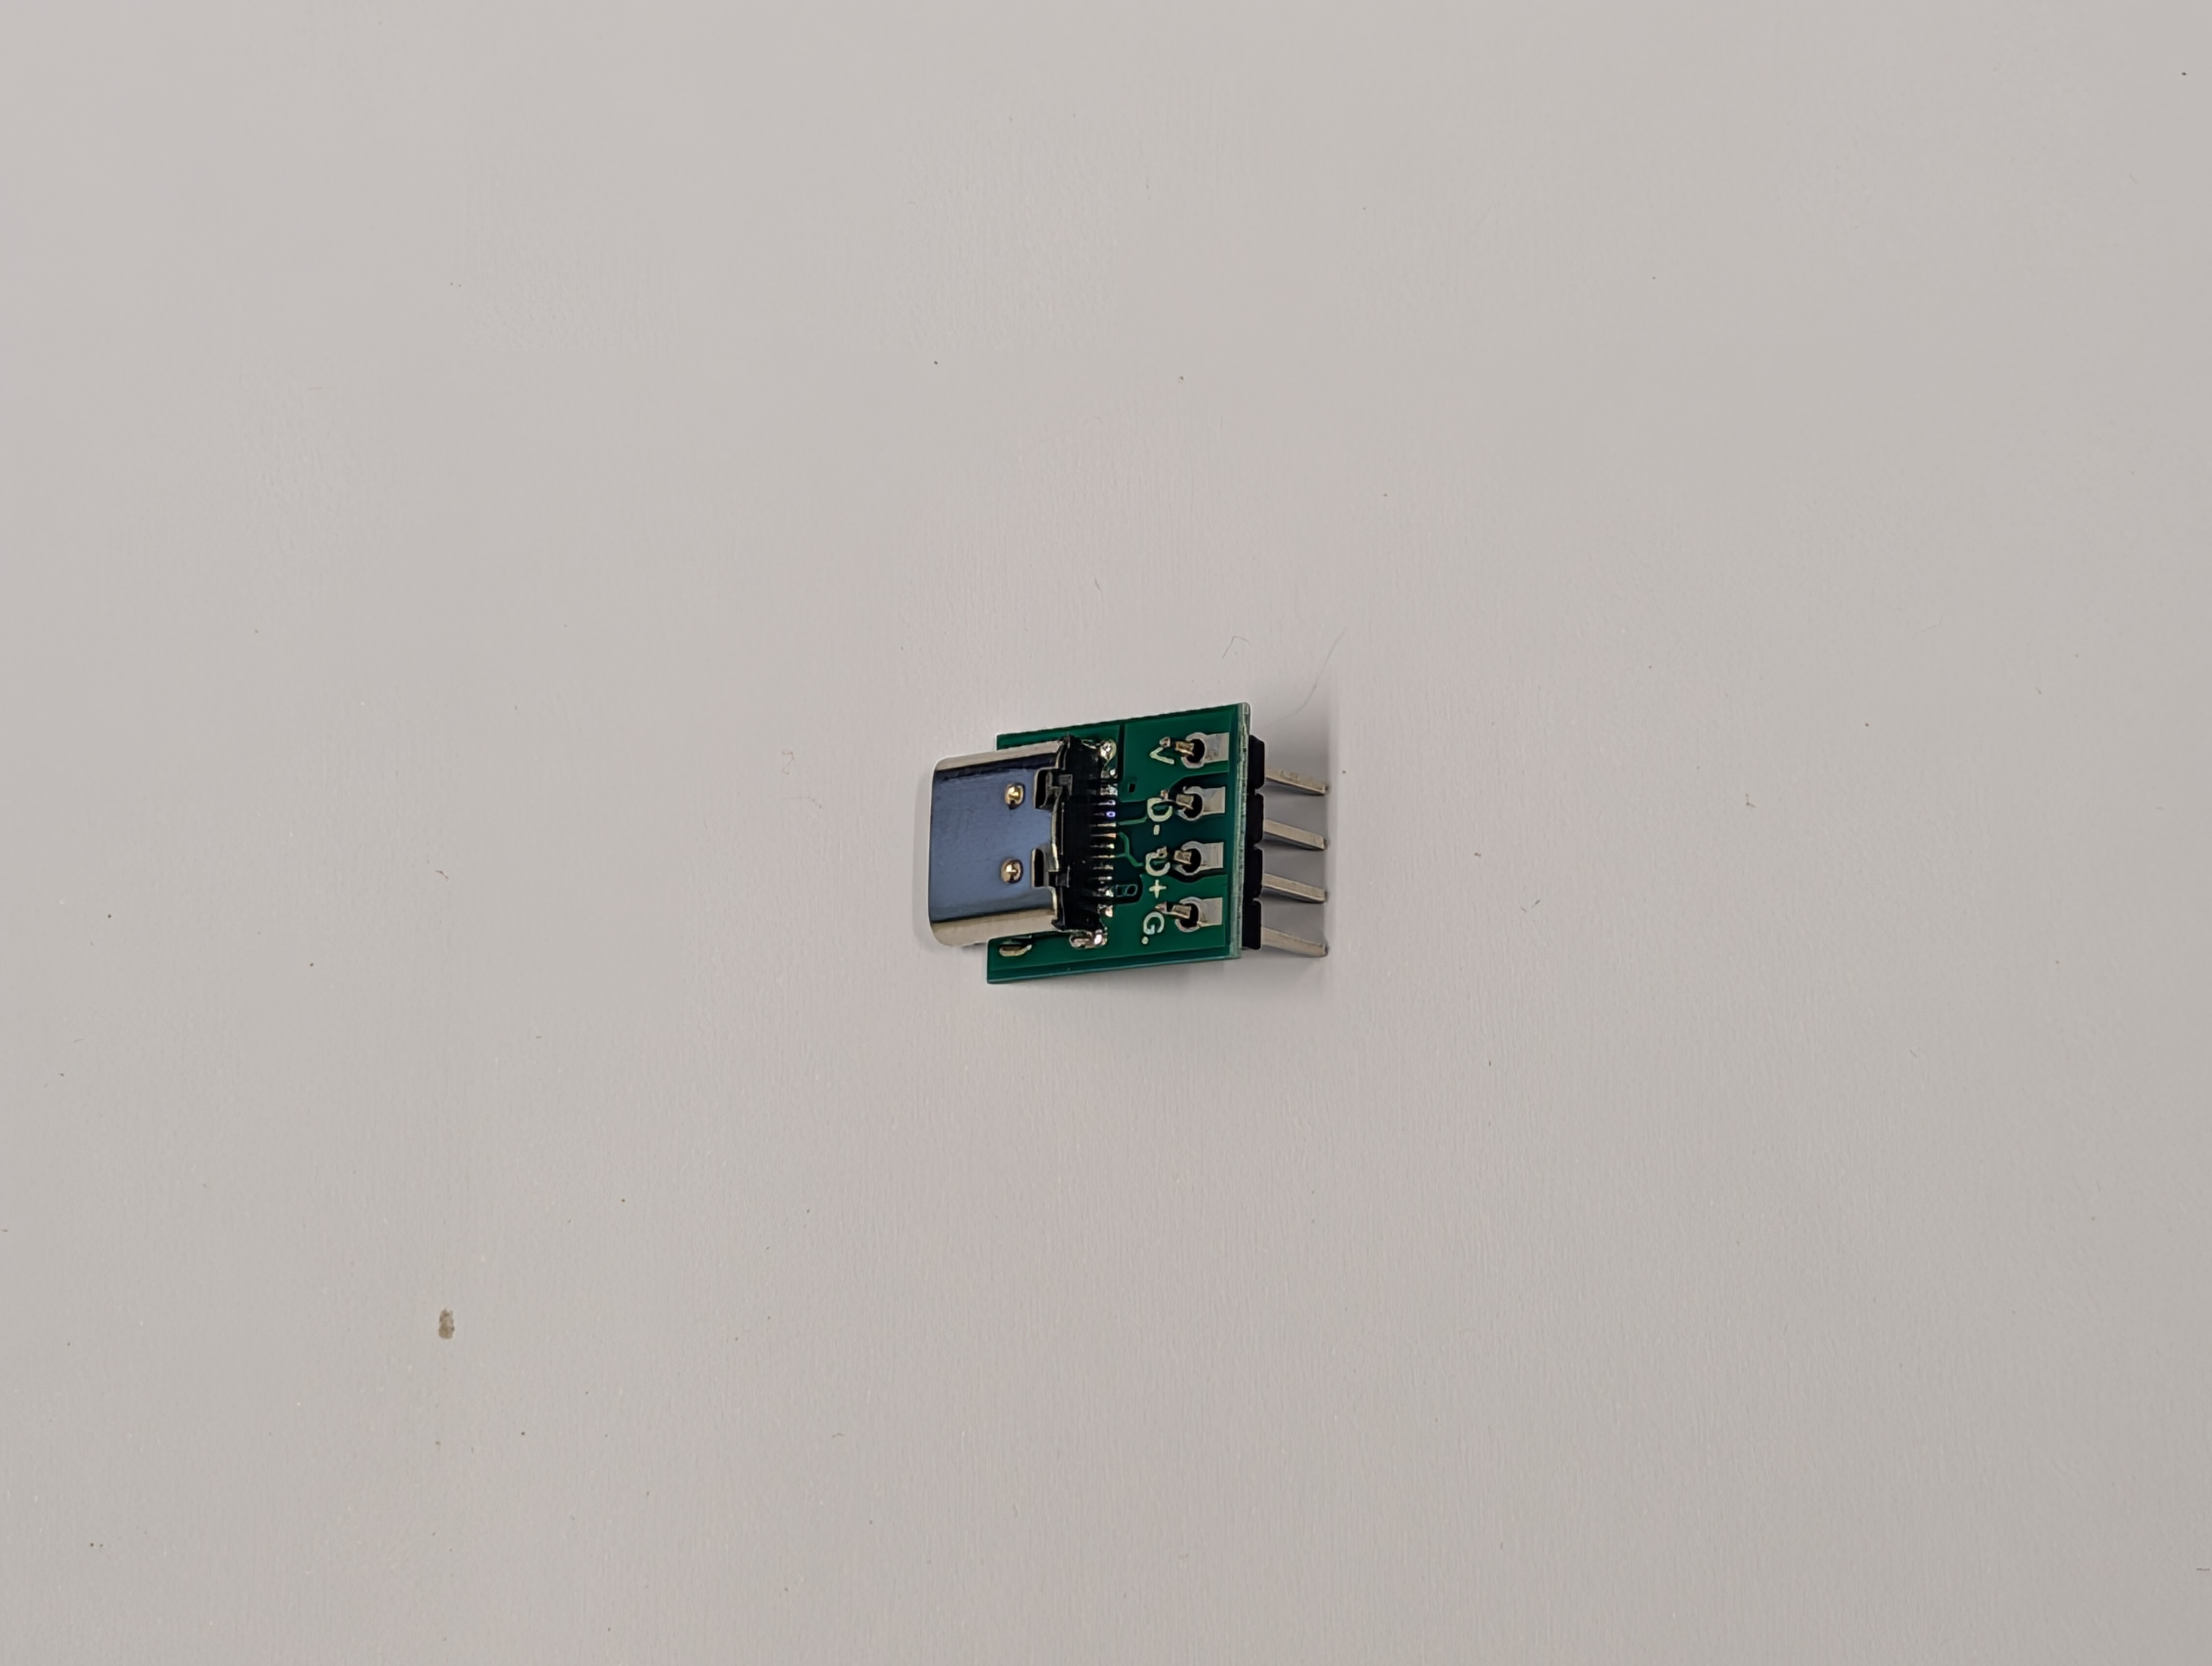
\includegraphics[width=0.75\textwidth]{pictures_of_construction/instruction_step_8.jpg}
\end{figure}

\begin{figure}[H]
    \centering
    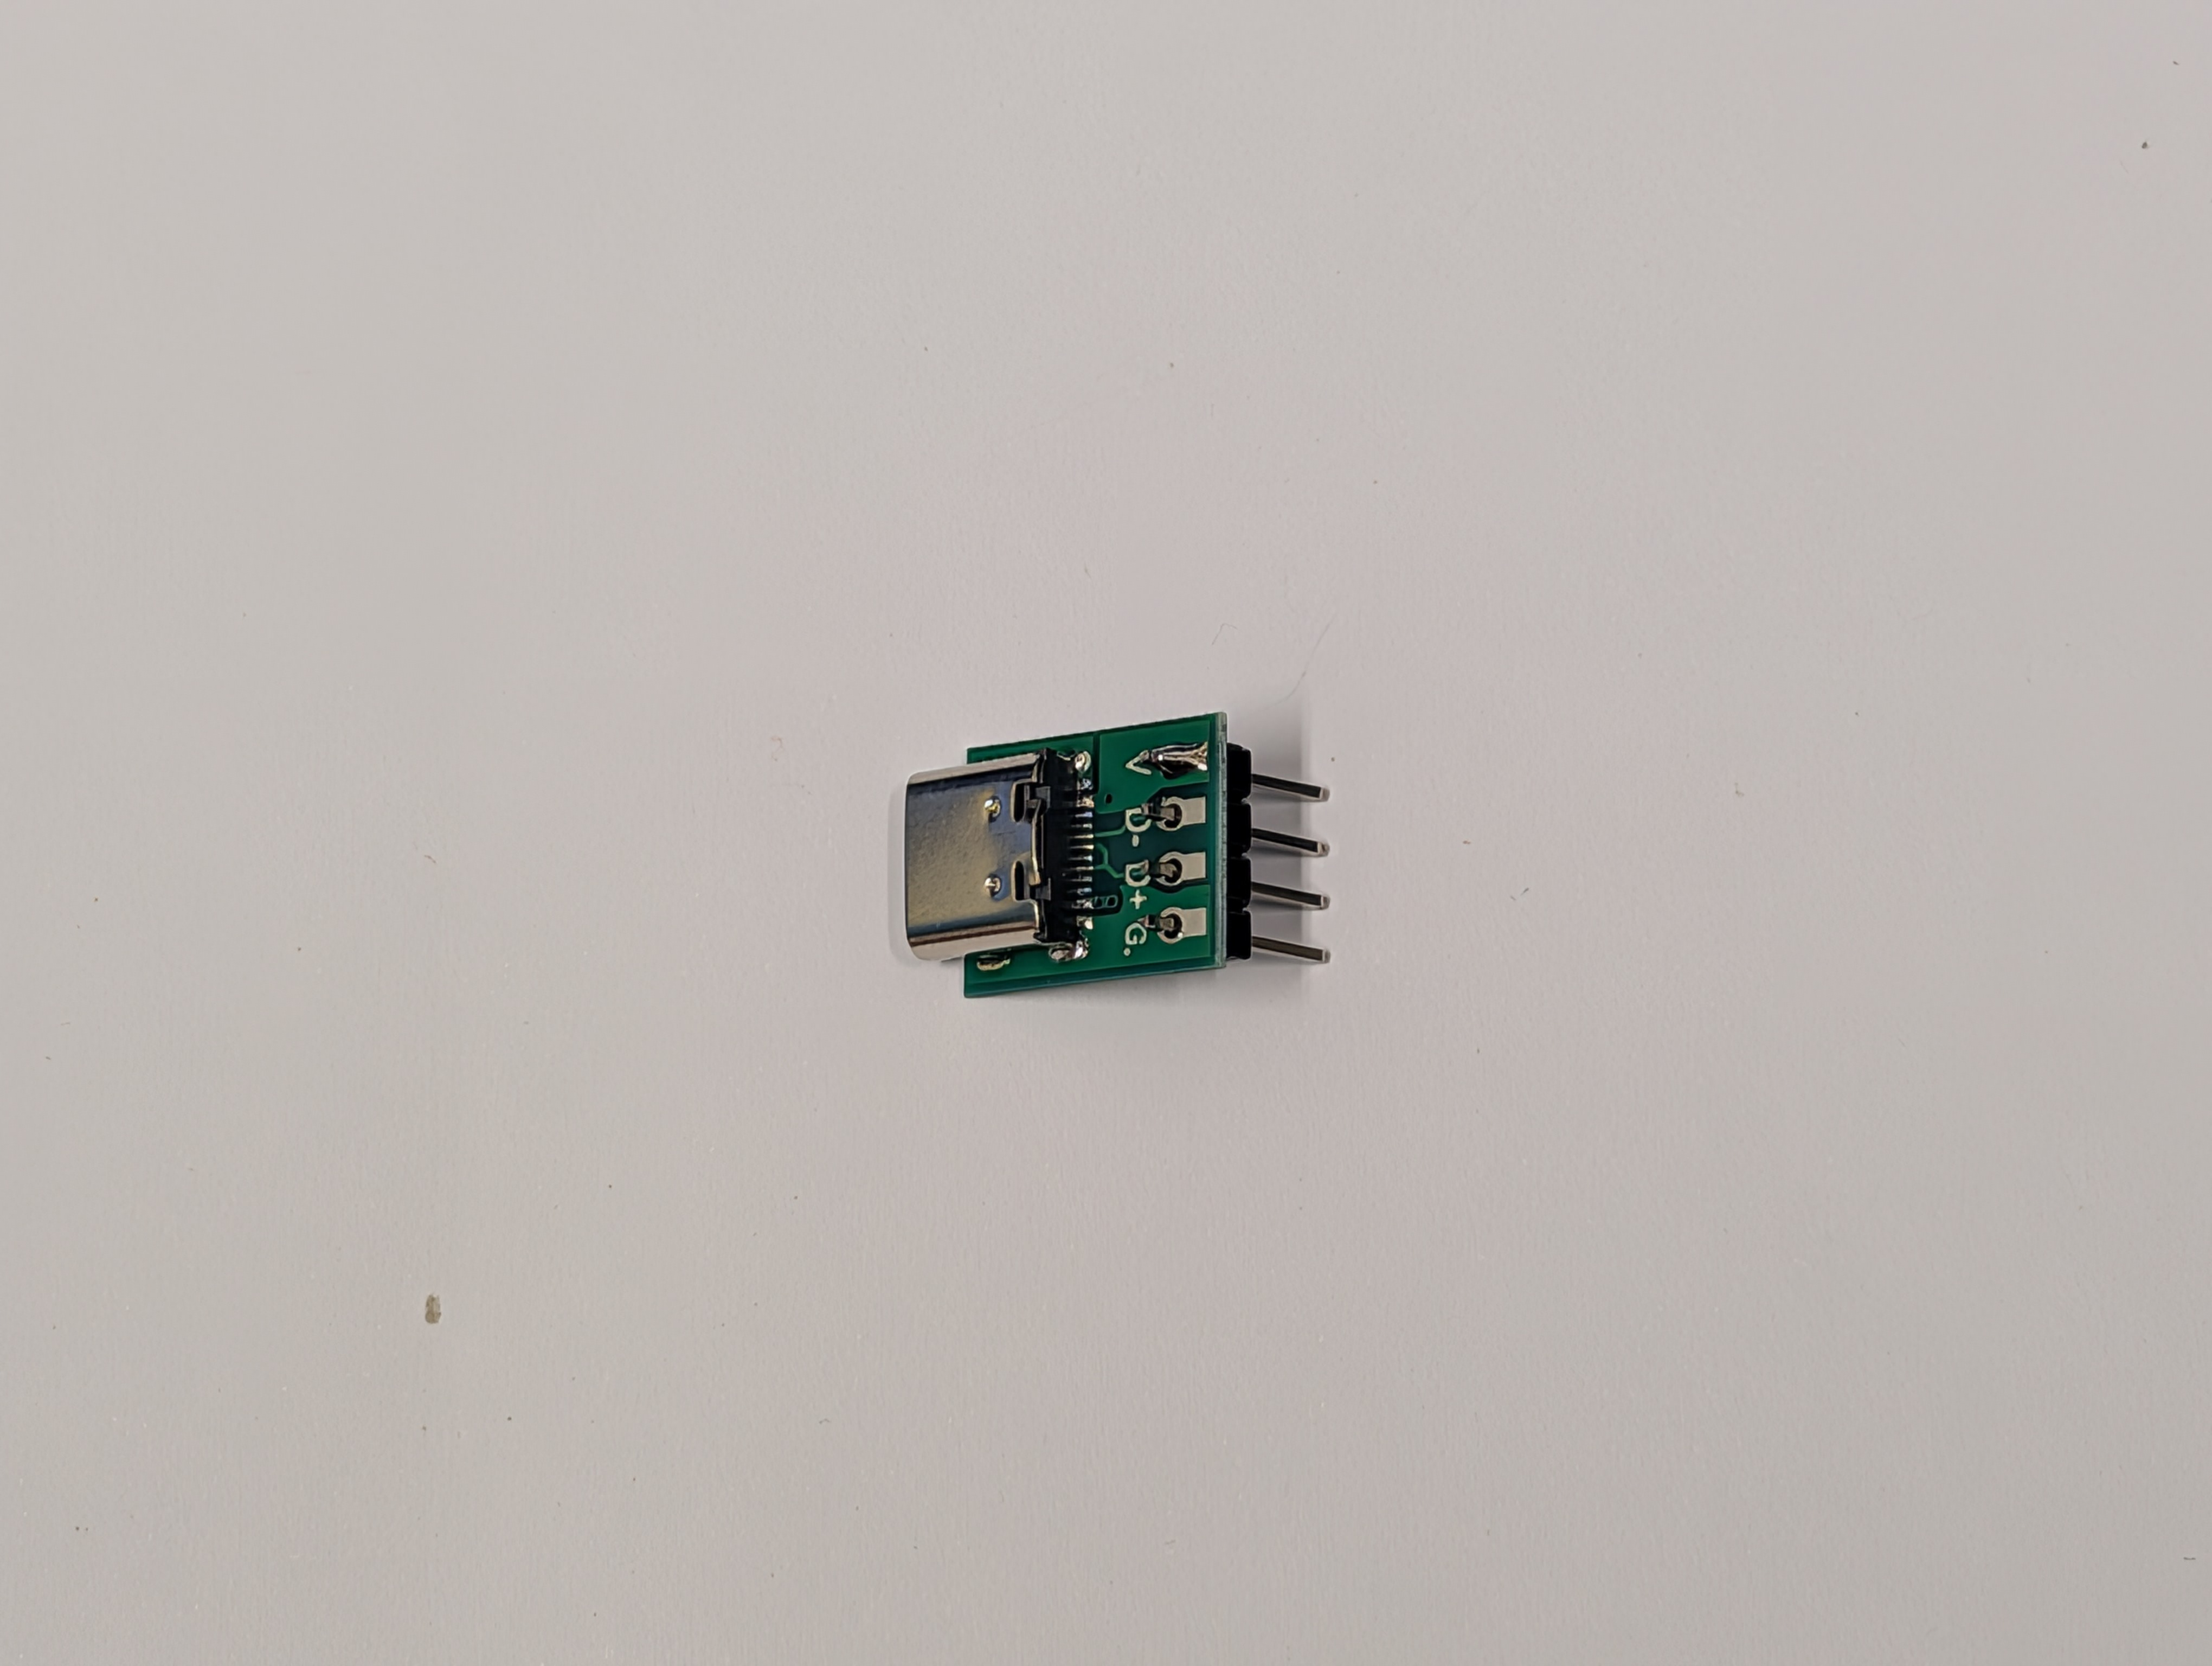
\includegraphics[width=0.75\textwidth]{pictures_of_construction/instruction_step_9.jpg}
\end{figure}

\begin{figure}[H]
    \centering
    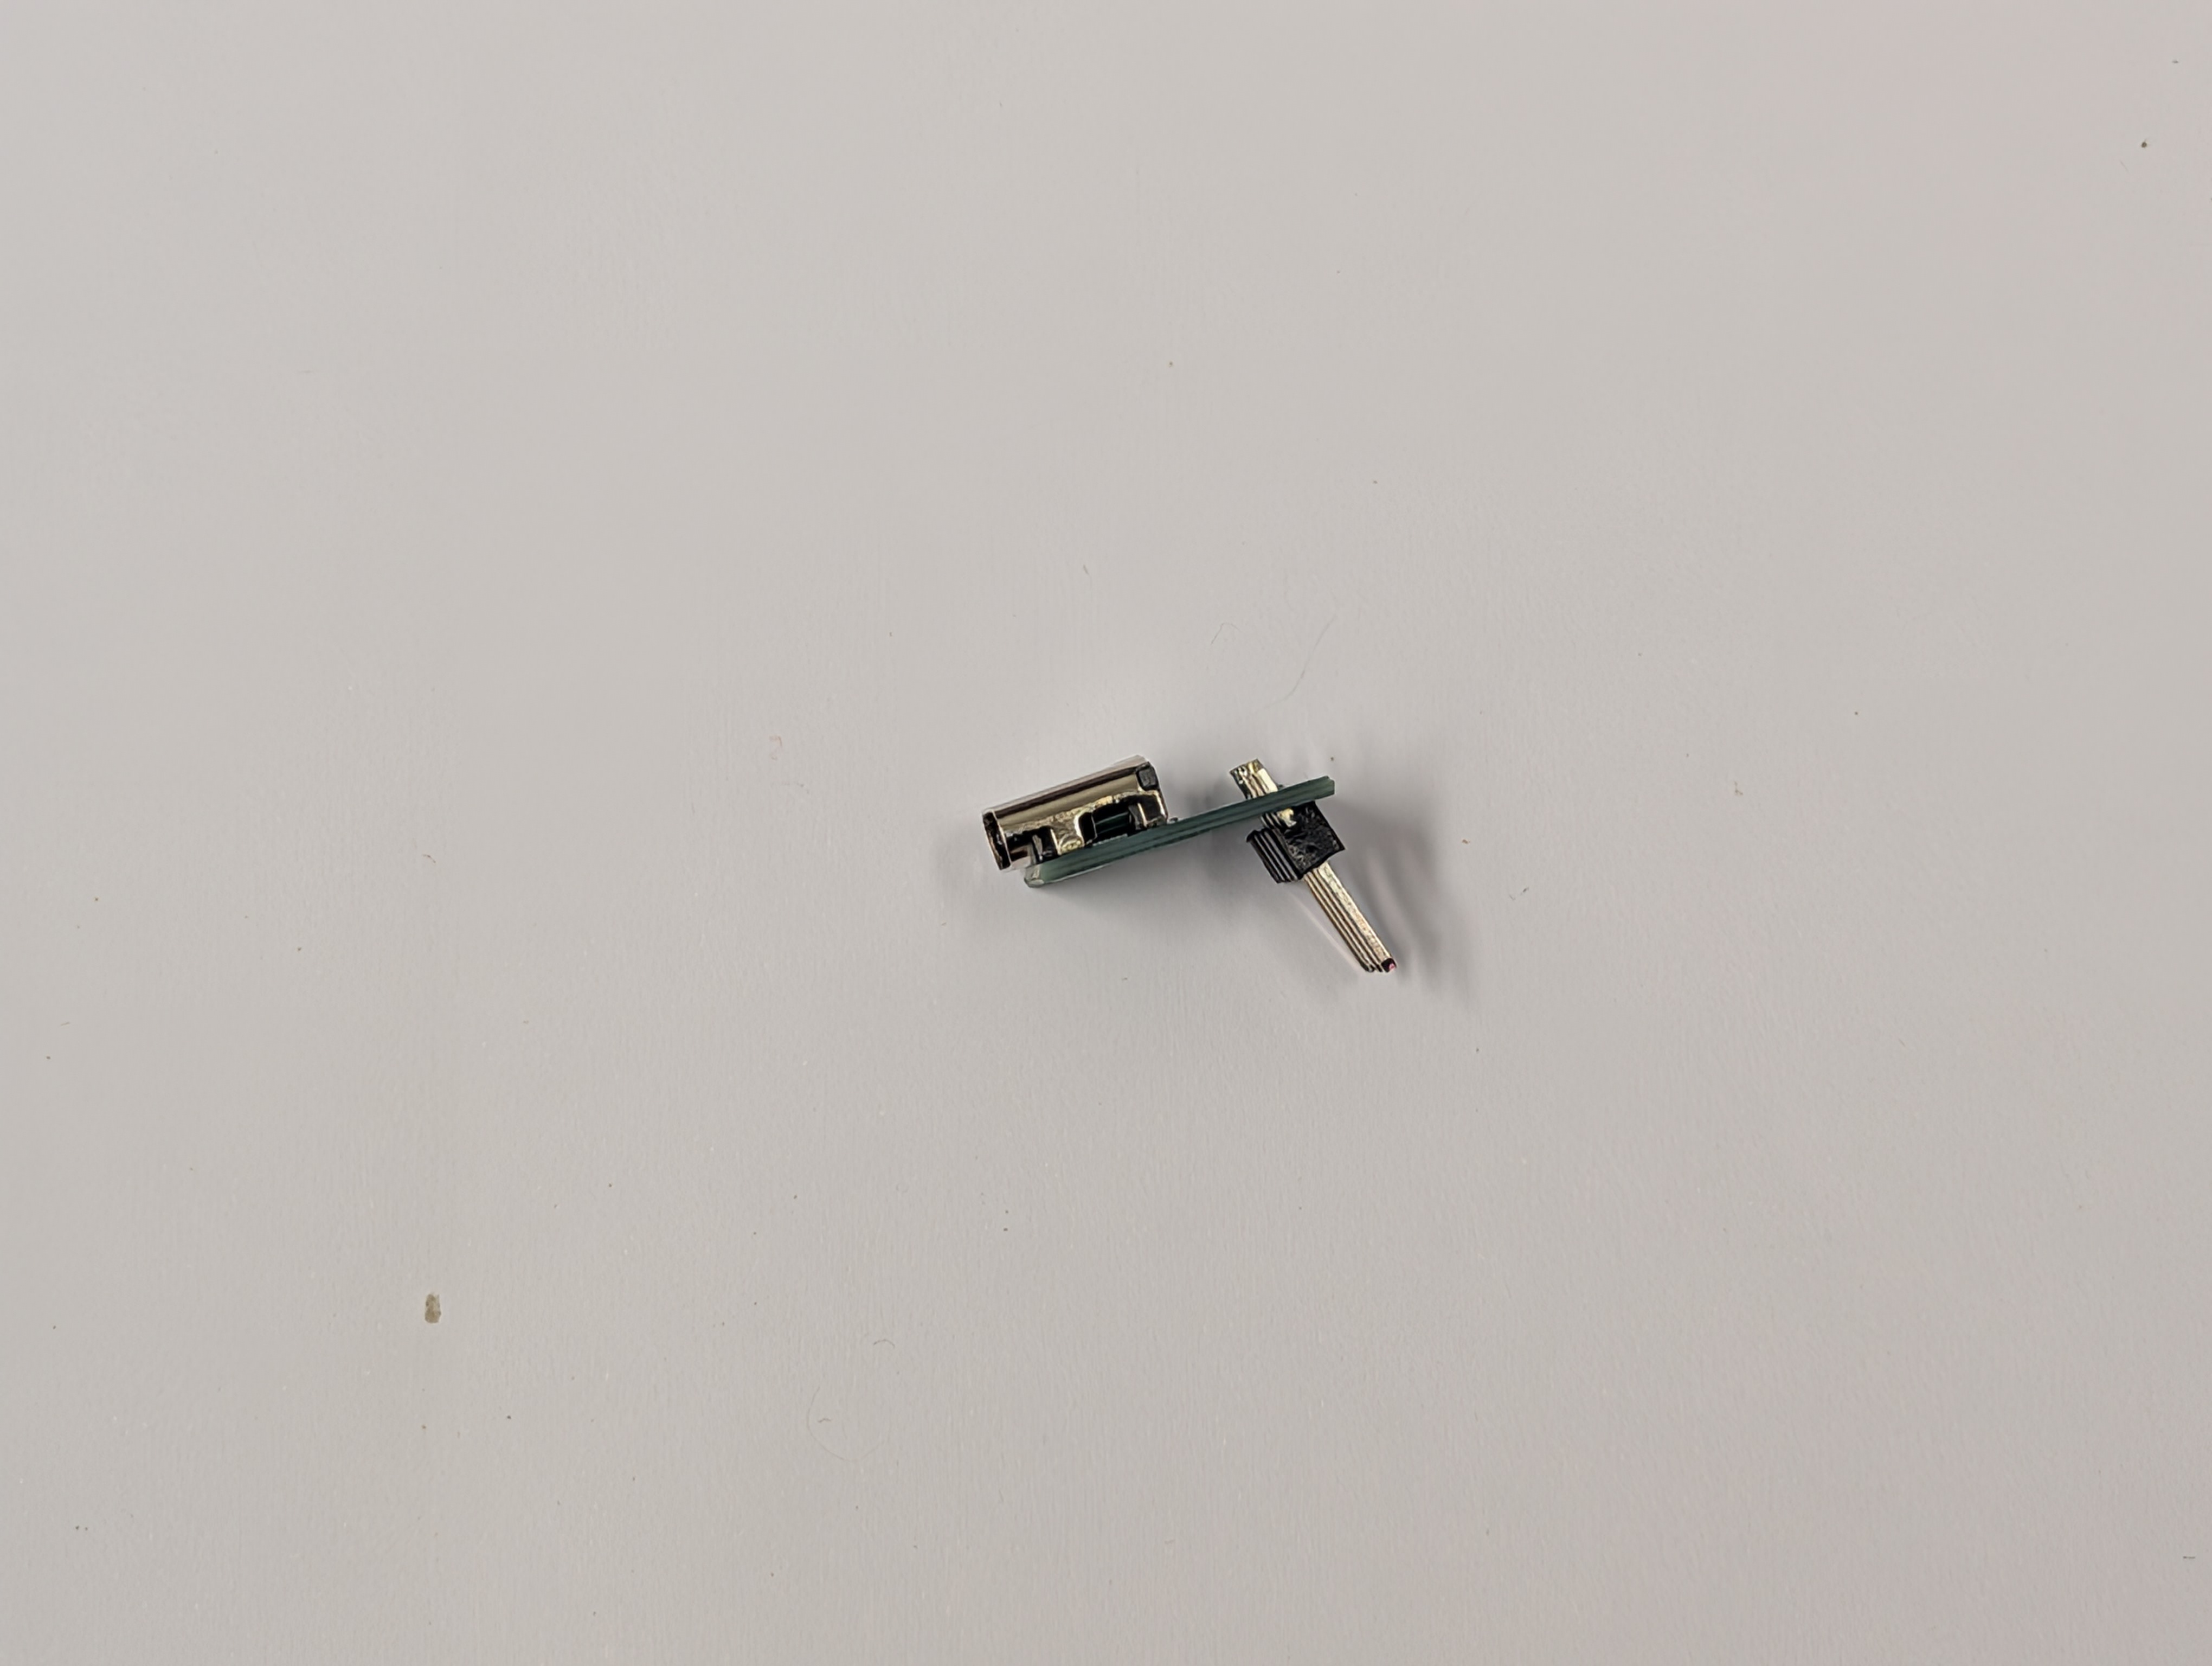
\includegraphics[width=0.75\textwidth]{pictures_of_construction/instruction_step_10.jpg}
\end{figure}

\begin{figure}[H]
    \centering
    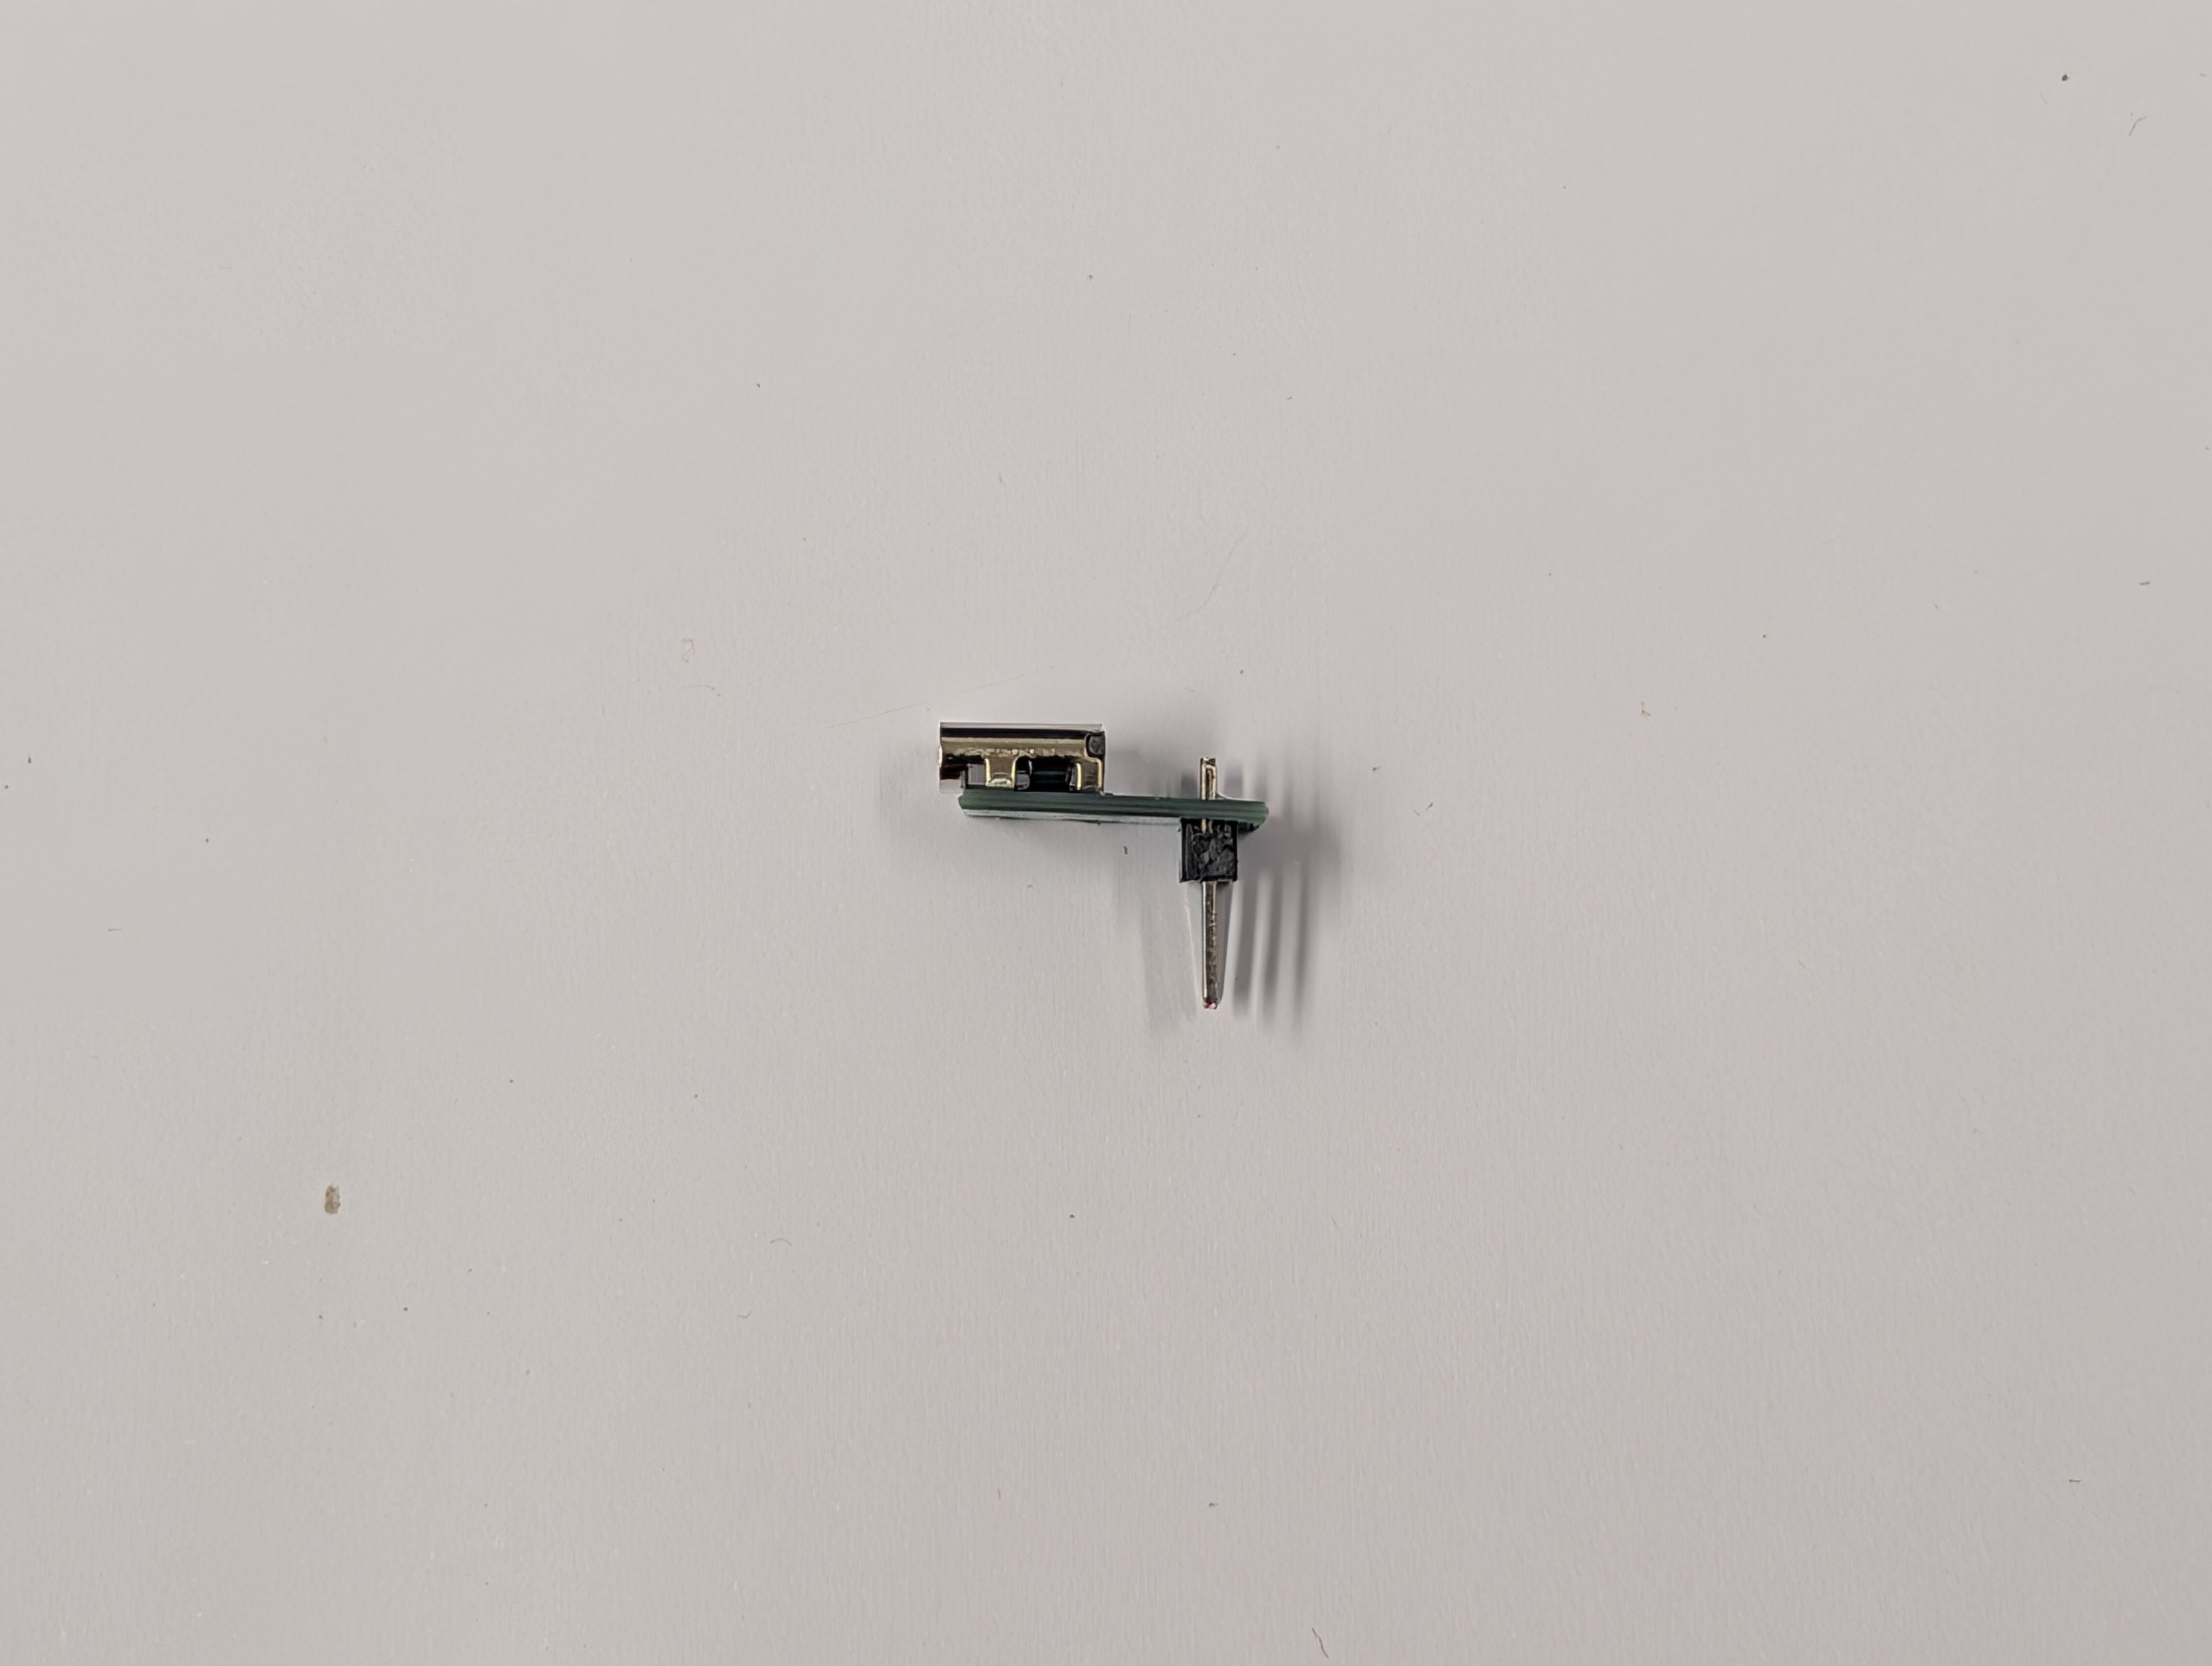
\includegraphics[width=0.75\textwidth]{pictures_of_construction/instruction_step_11.jpg}
\end{figure}

\subsection*{3. AHT10-Sensor vorbereiten}

Der AHT10-Sensor wird fast genauso vorbereitet wie das USB-C-Breakout-Board.

\begin{figure}[H]
    \centering
    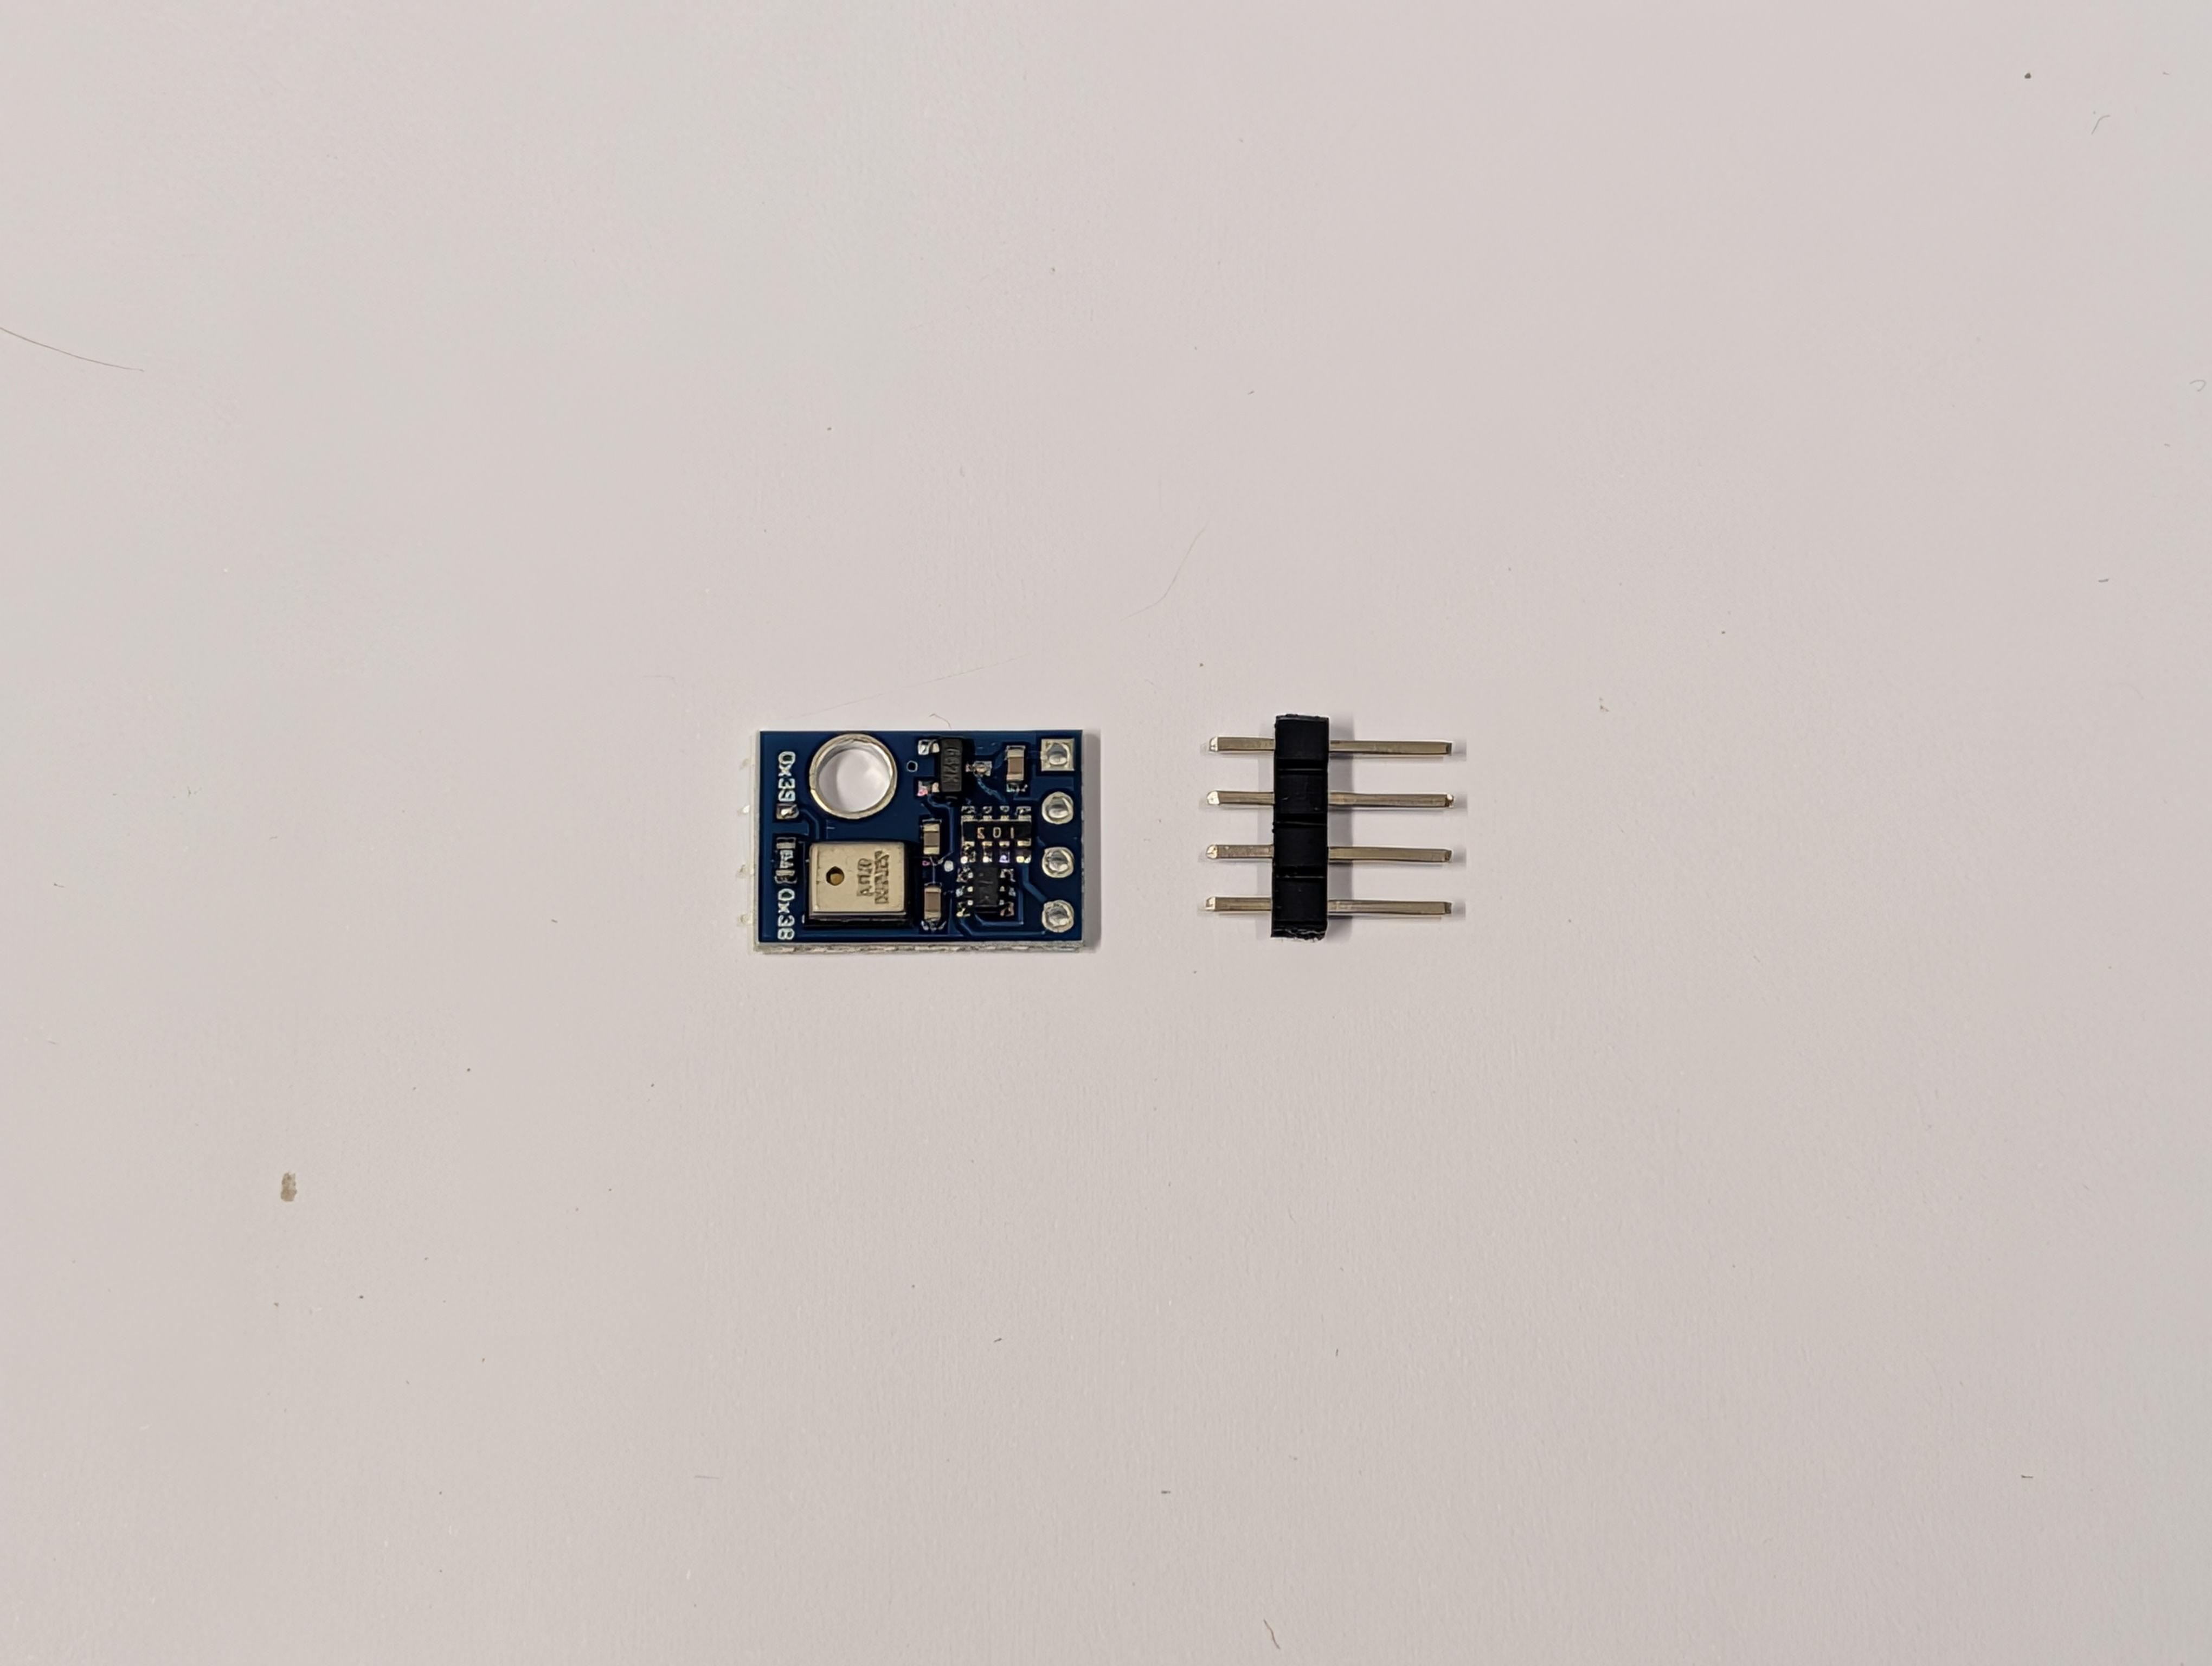
\includegraphics[width=0.75\textwidth]{pictures_of_construction/instruction_step_12.jpg}
\end{figure}

So geht’s:
\begin{enumerate}
    \item Stiftleiste einstecken.
    \item Einen Pin löten.
    \item Gerade ausrichten.
    \item Alle Pins fertig löten.
\end{enumerate}

\begin{figure}[H]
    \centering
    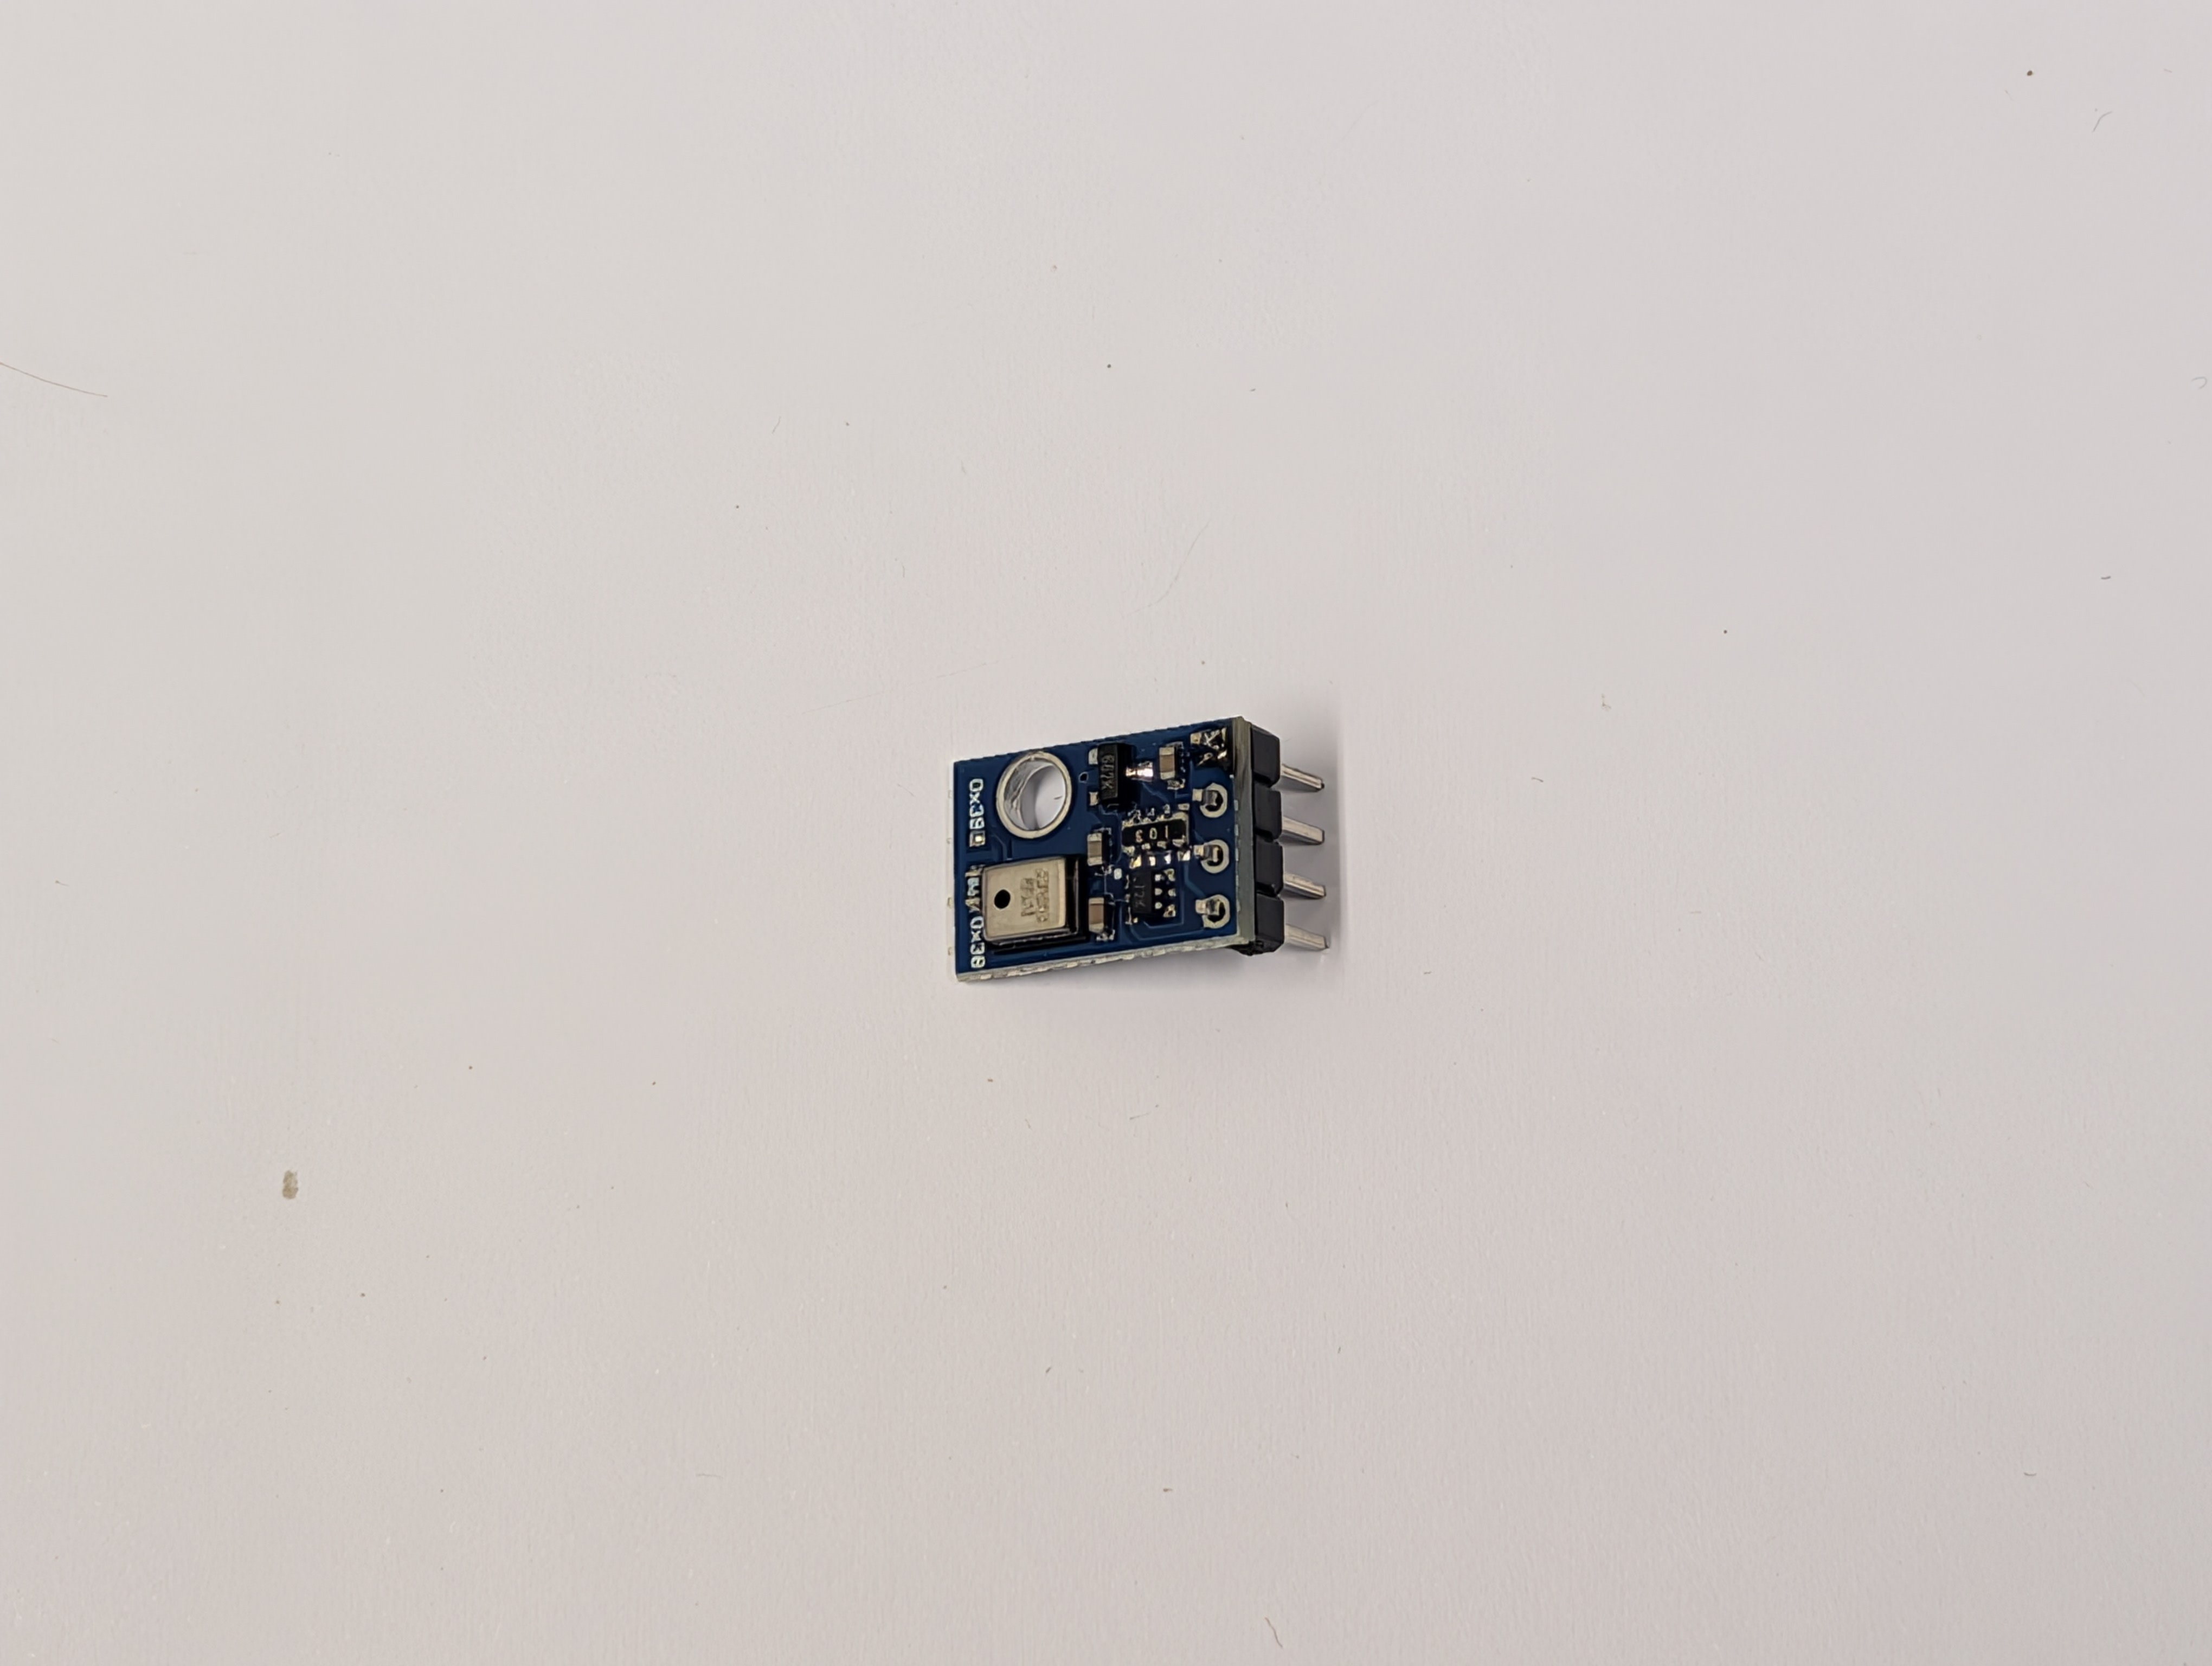
\includegraphics[width=0.75\textwidth]{pictures_of_construction/instruction_step_13.jpg}
\end{figure}

\subsection*{4. LCD-Display vorbereiten}

Auch das Display bekommt zuerst seine Stiftleiste.

\begin{figure}[H]
    \centering
    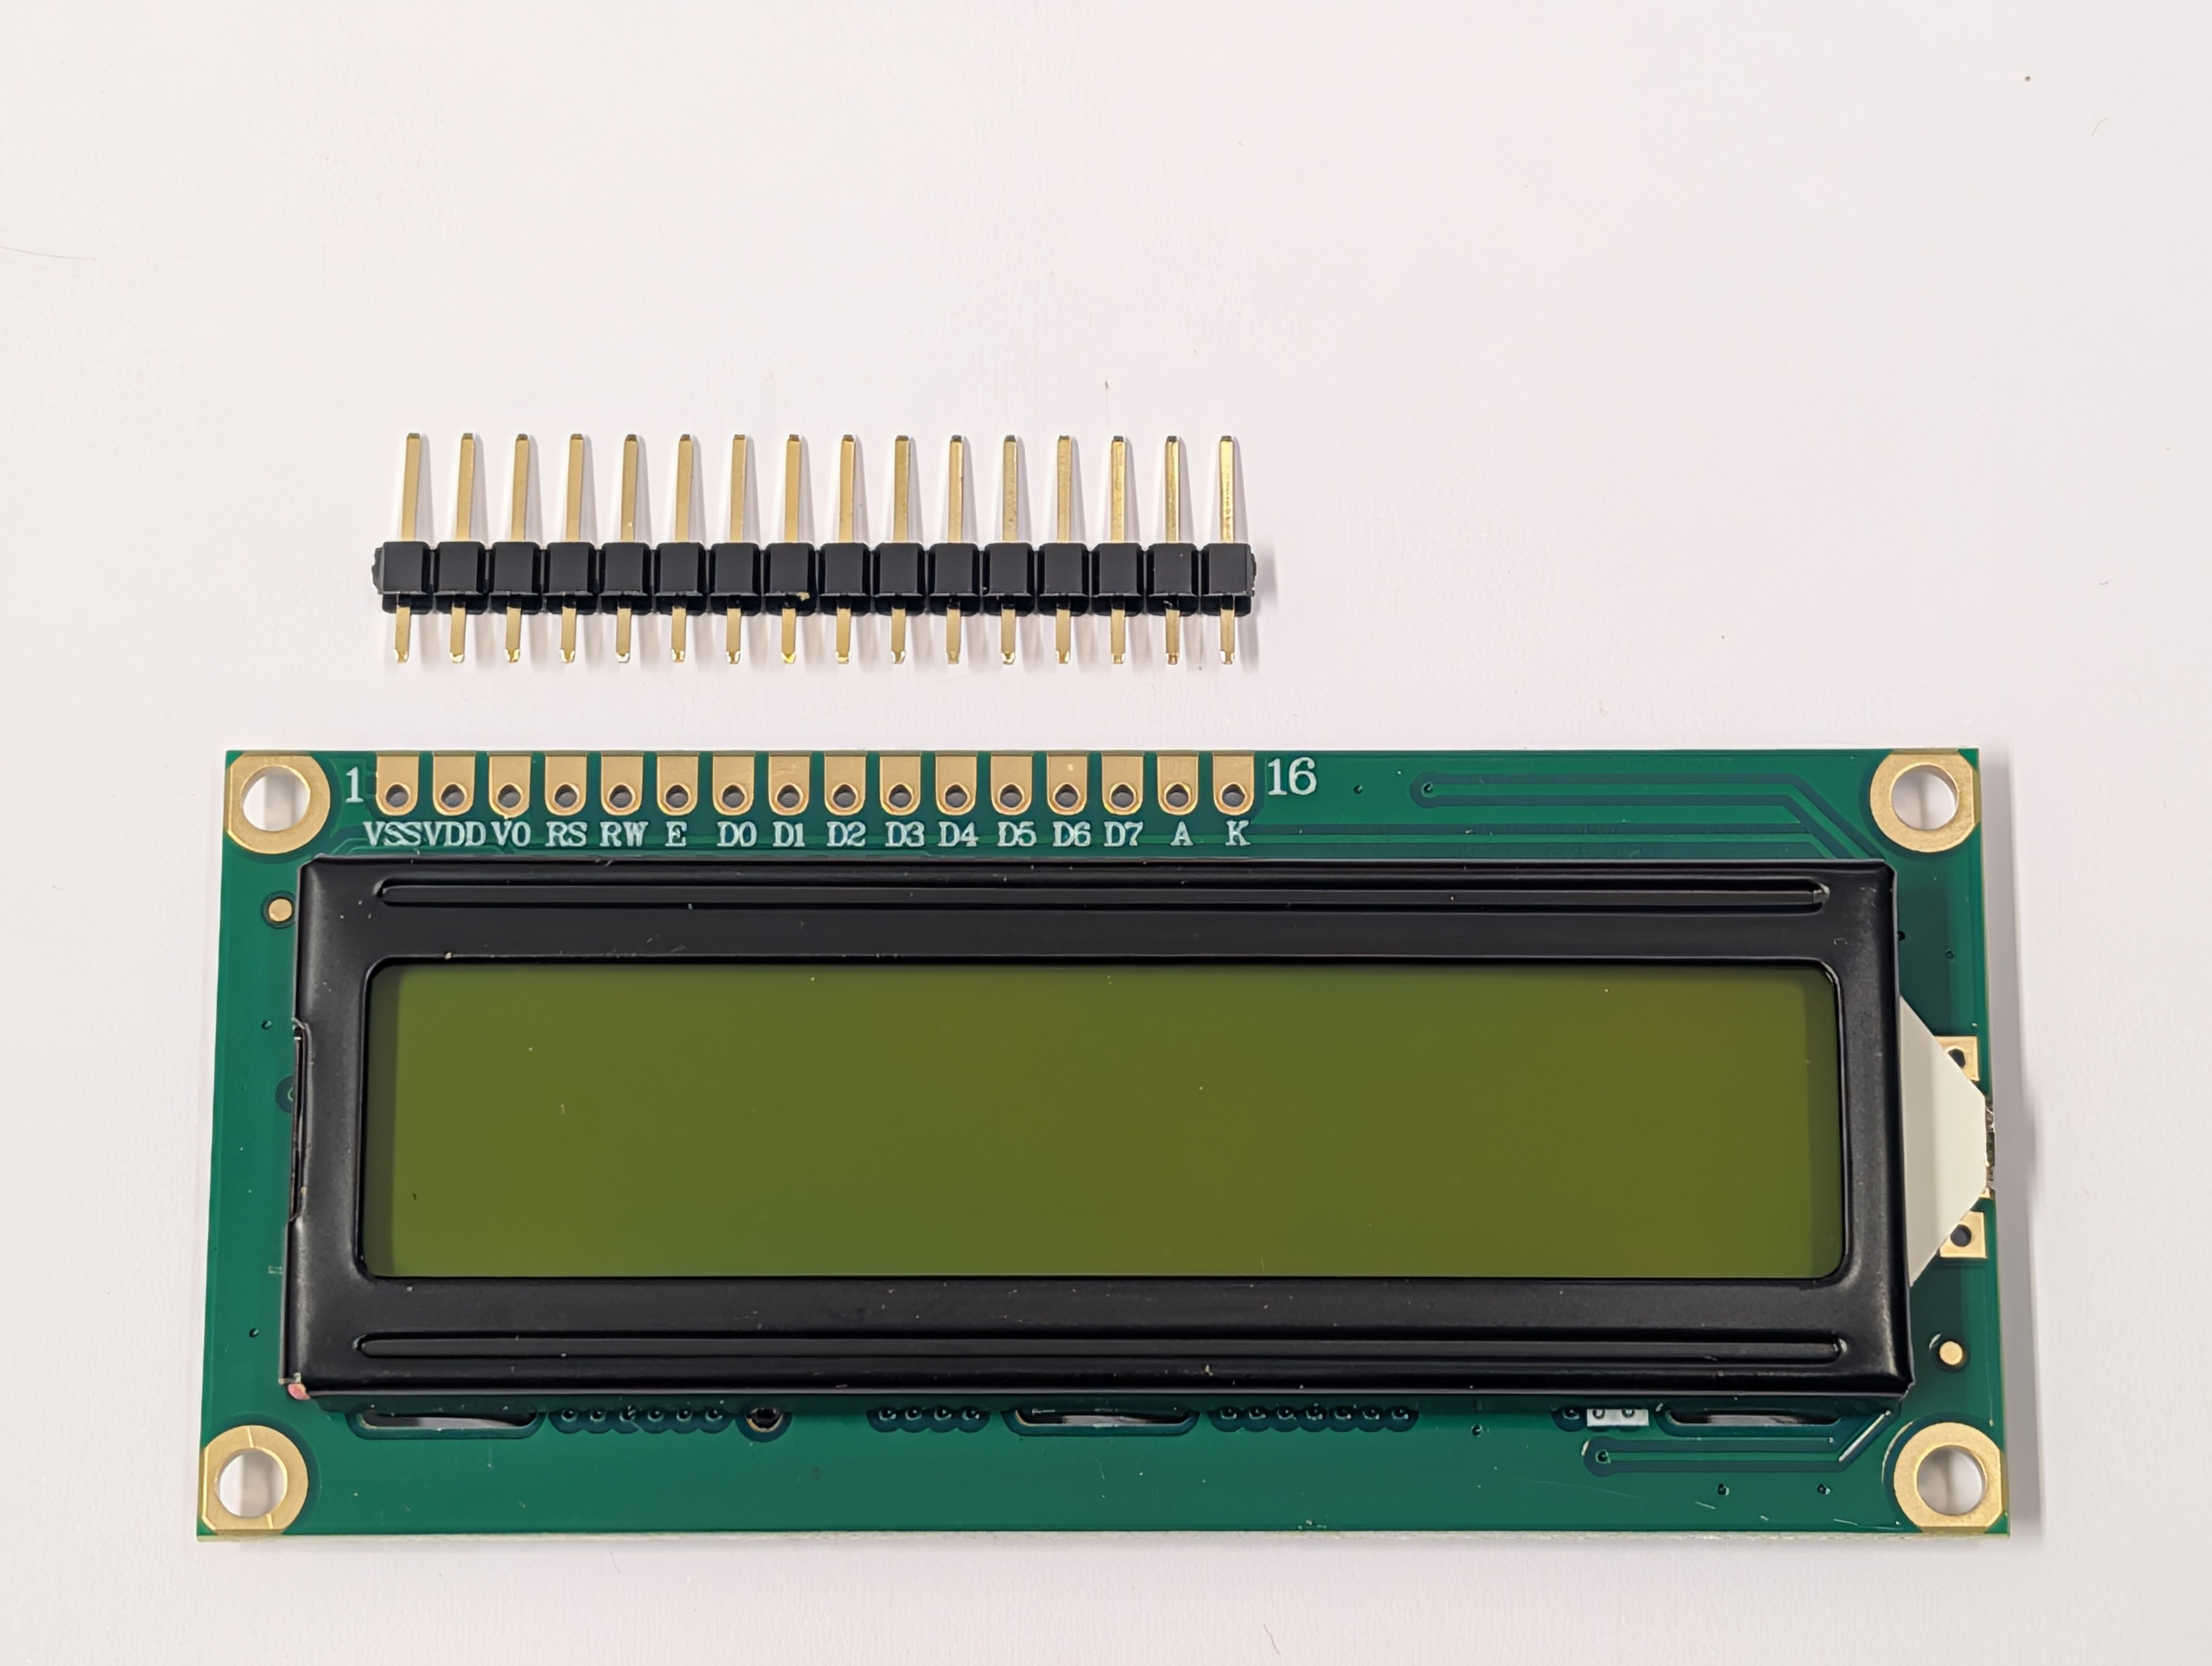
\includegraphics[width=0.75\textwidth]{pictures_of_construction/instruction_step_14.jpg}
\end{figure}

So geht’s:
\begin{enumerate}
    \item Stiftleiste einstecken.
    \item Einen Pin löten.
    \item Prüfen, ob alles gerade ist.
    \item Alle Pins festlöten.
\end{enumerate}

\begin{figure}[H]
    \centering
    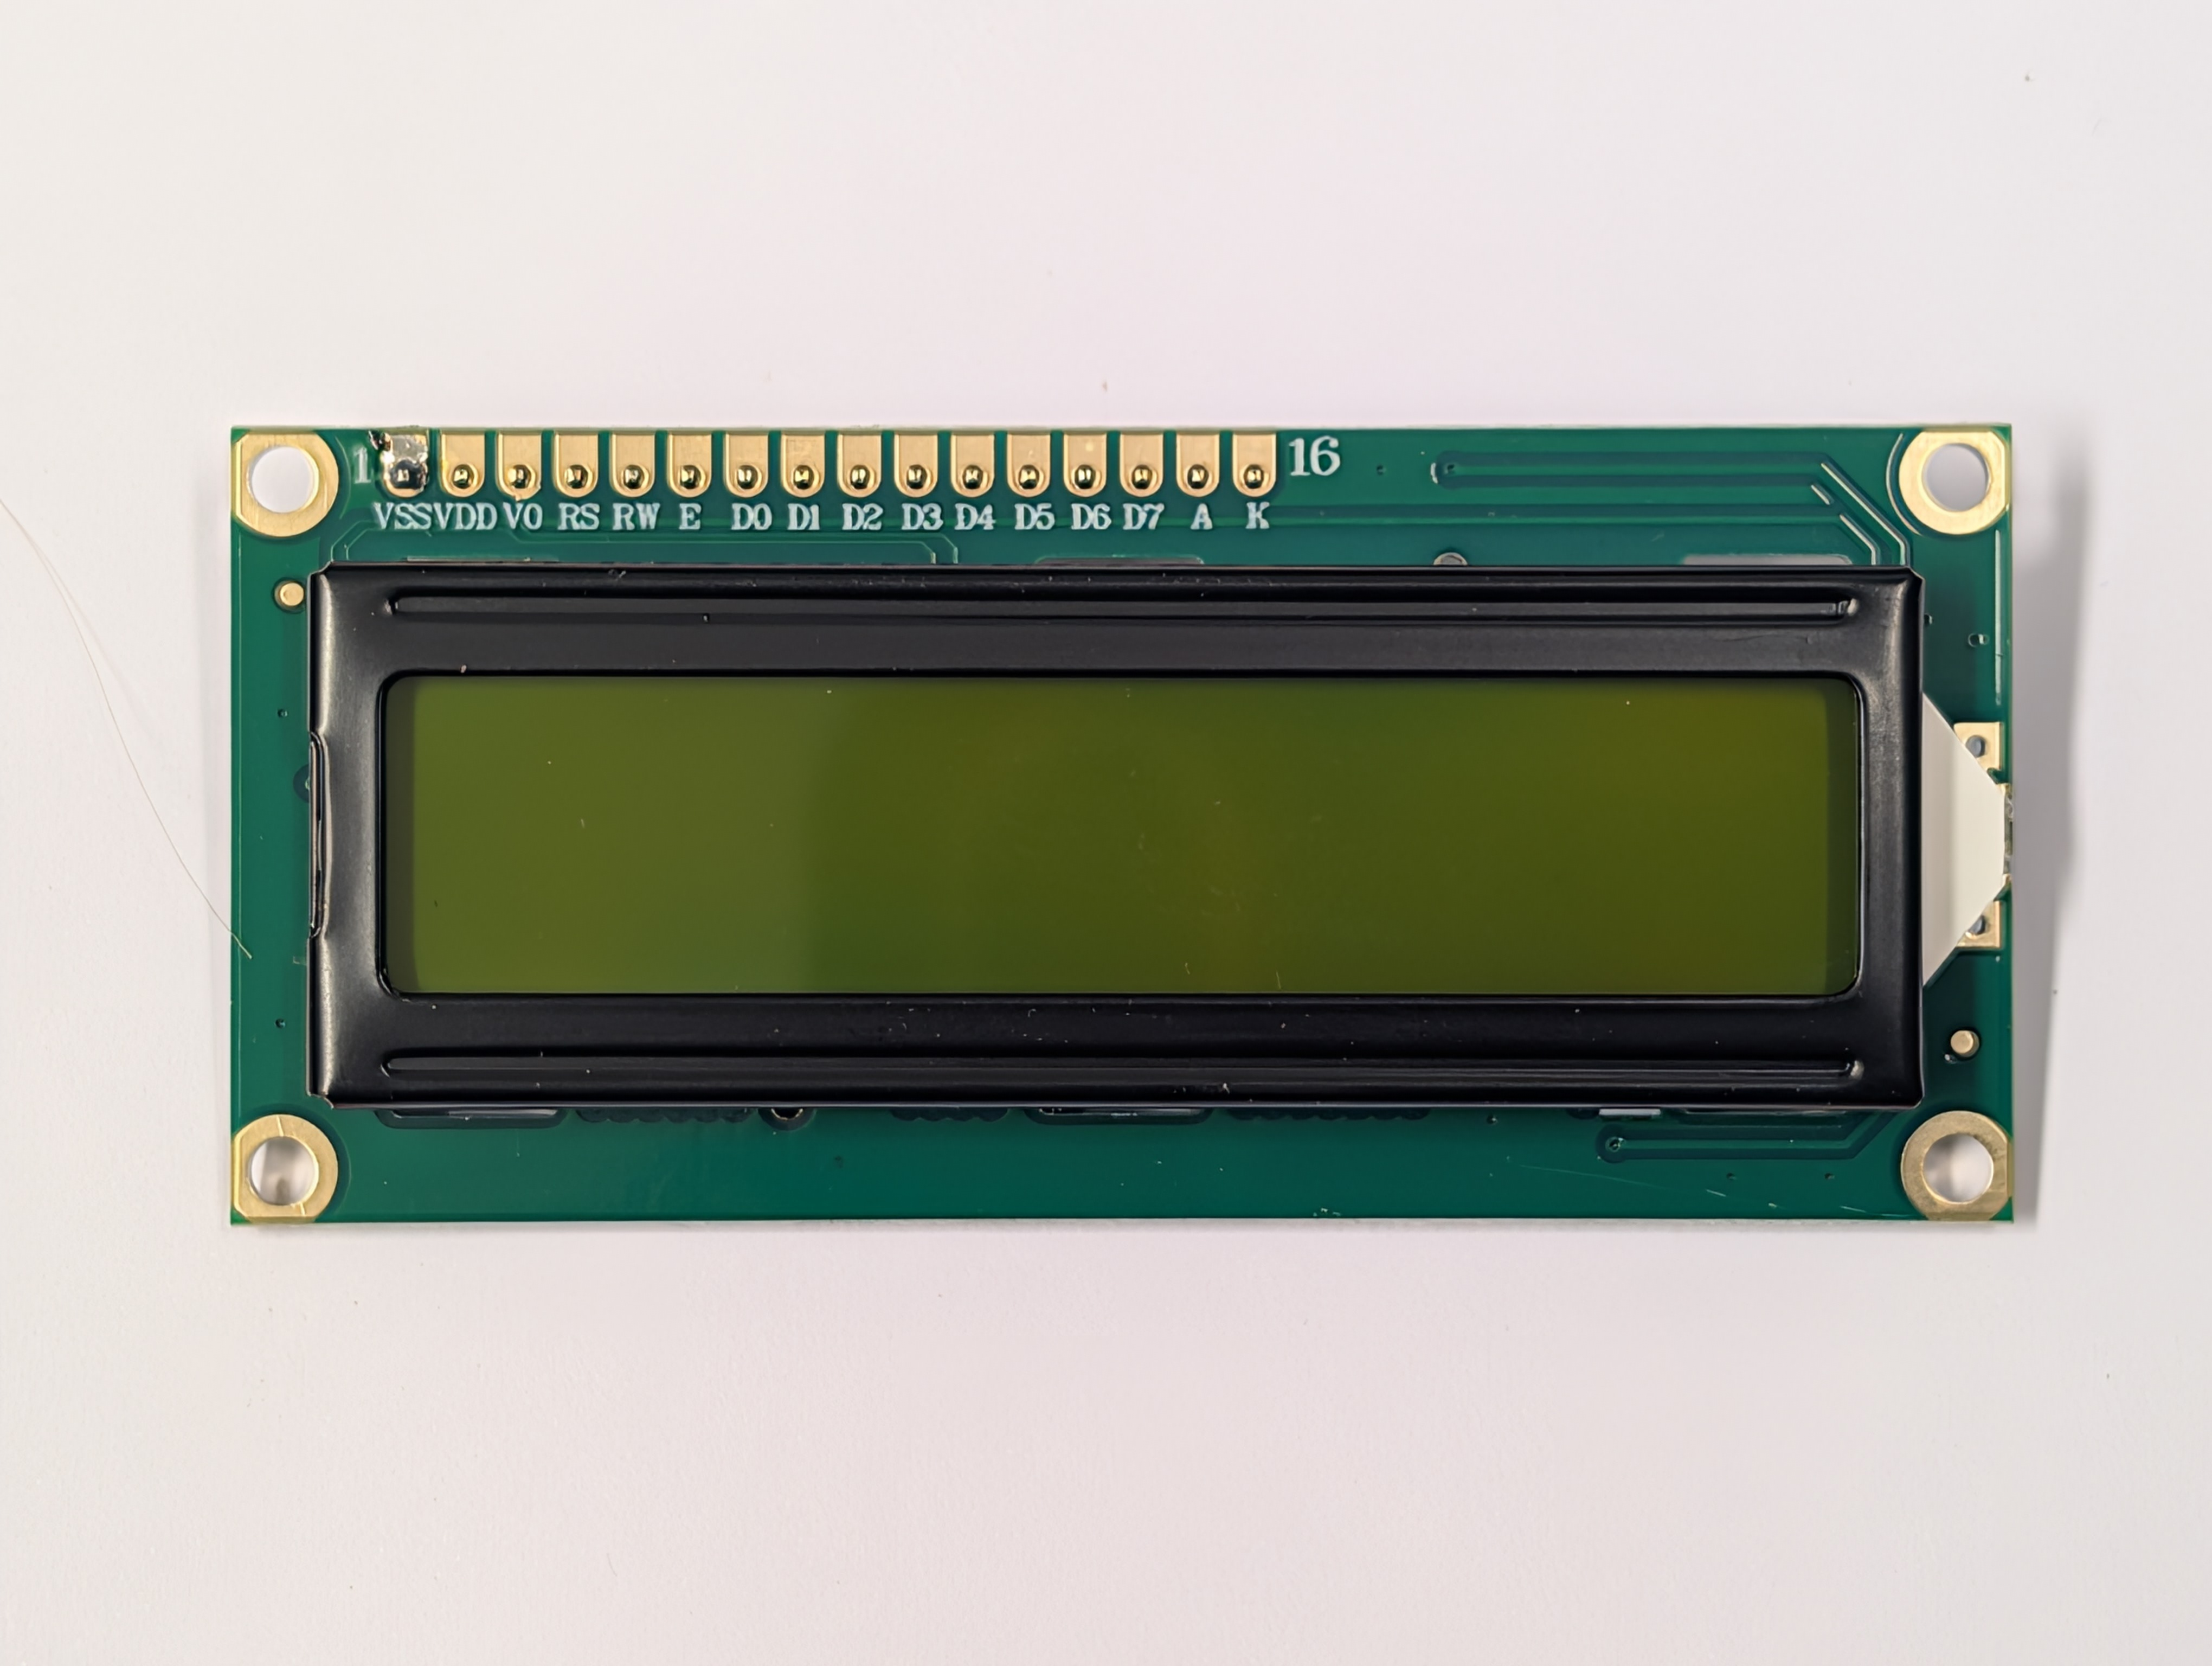
\includegraphics[width=0.75\textwidth]{pictures_of_construction/instruction_step_15.jpg}
\end{figure}

\begin{figure}[H]
    \centering
    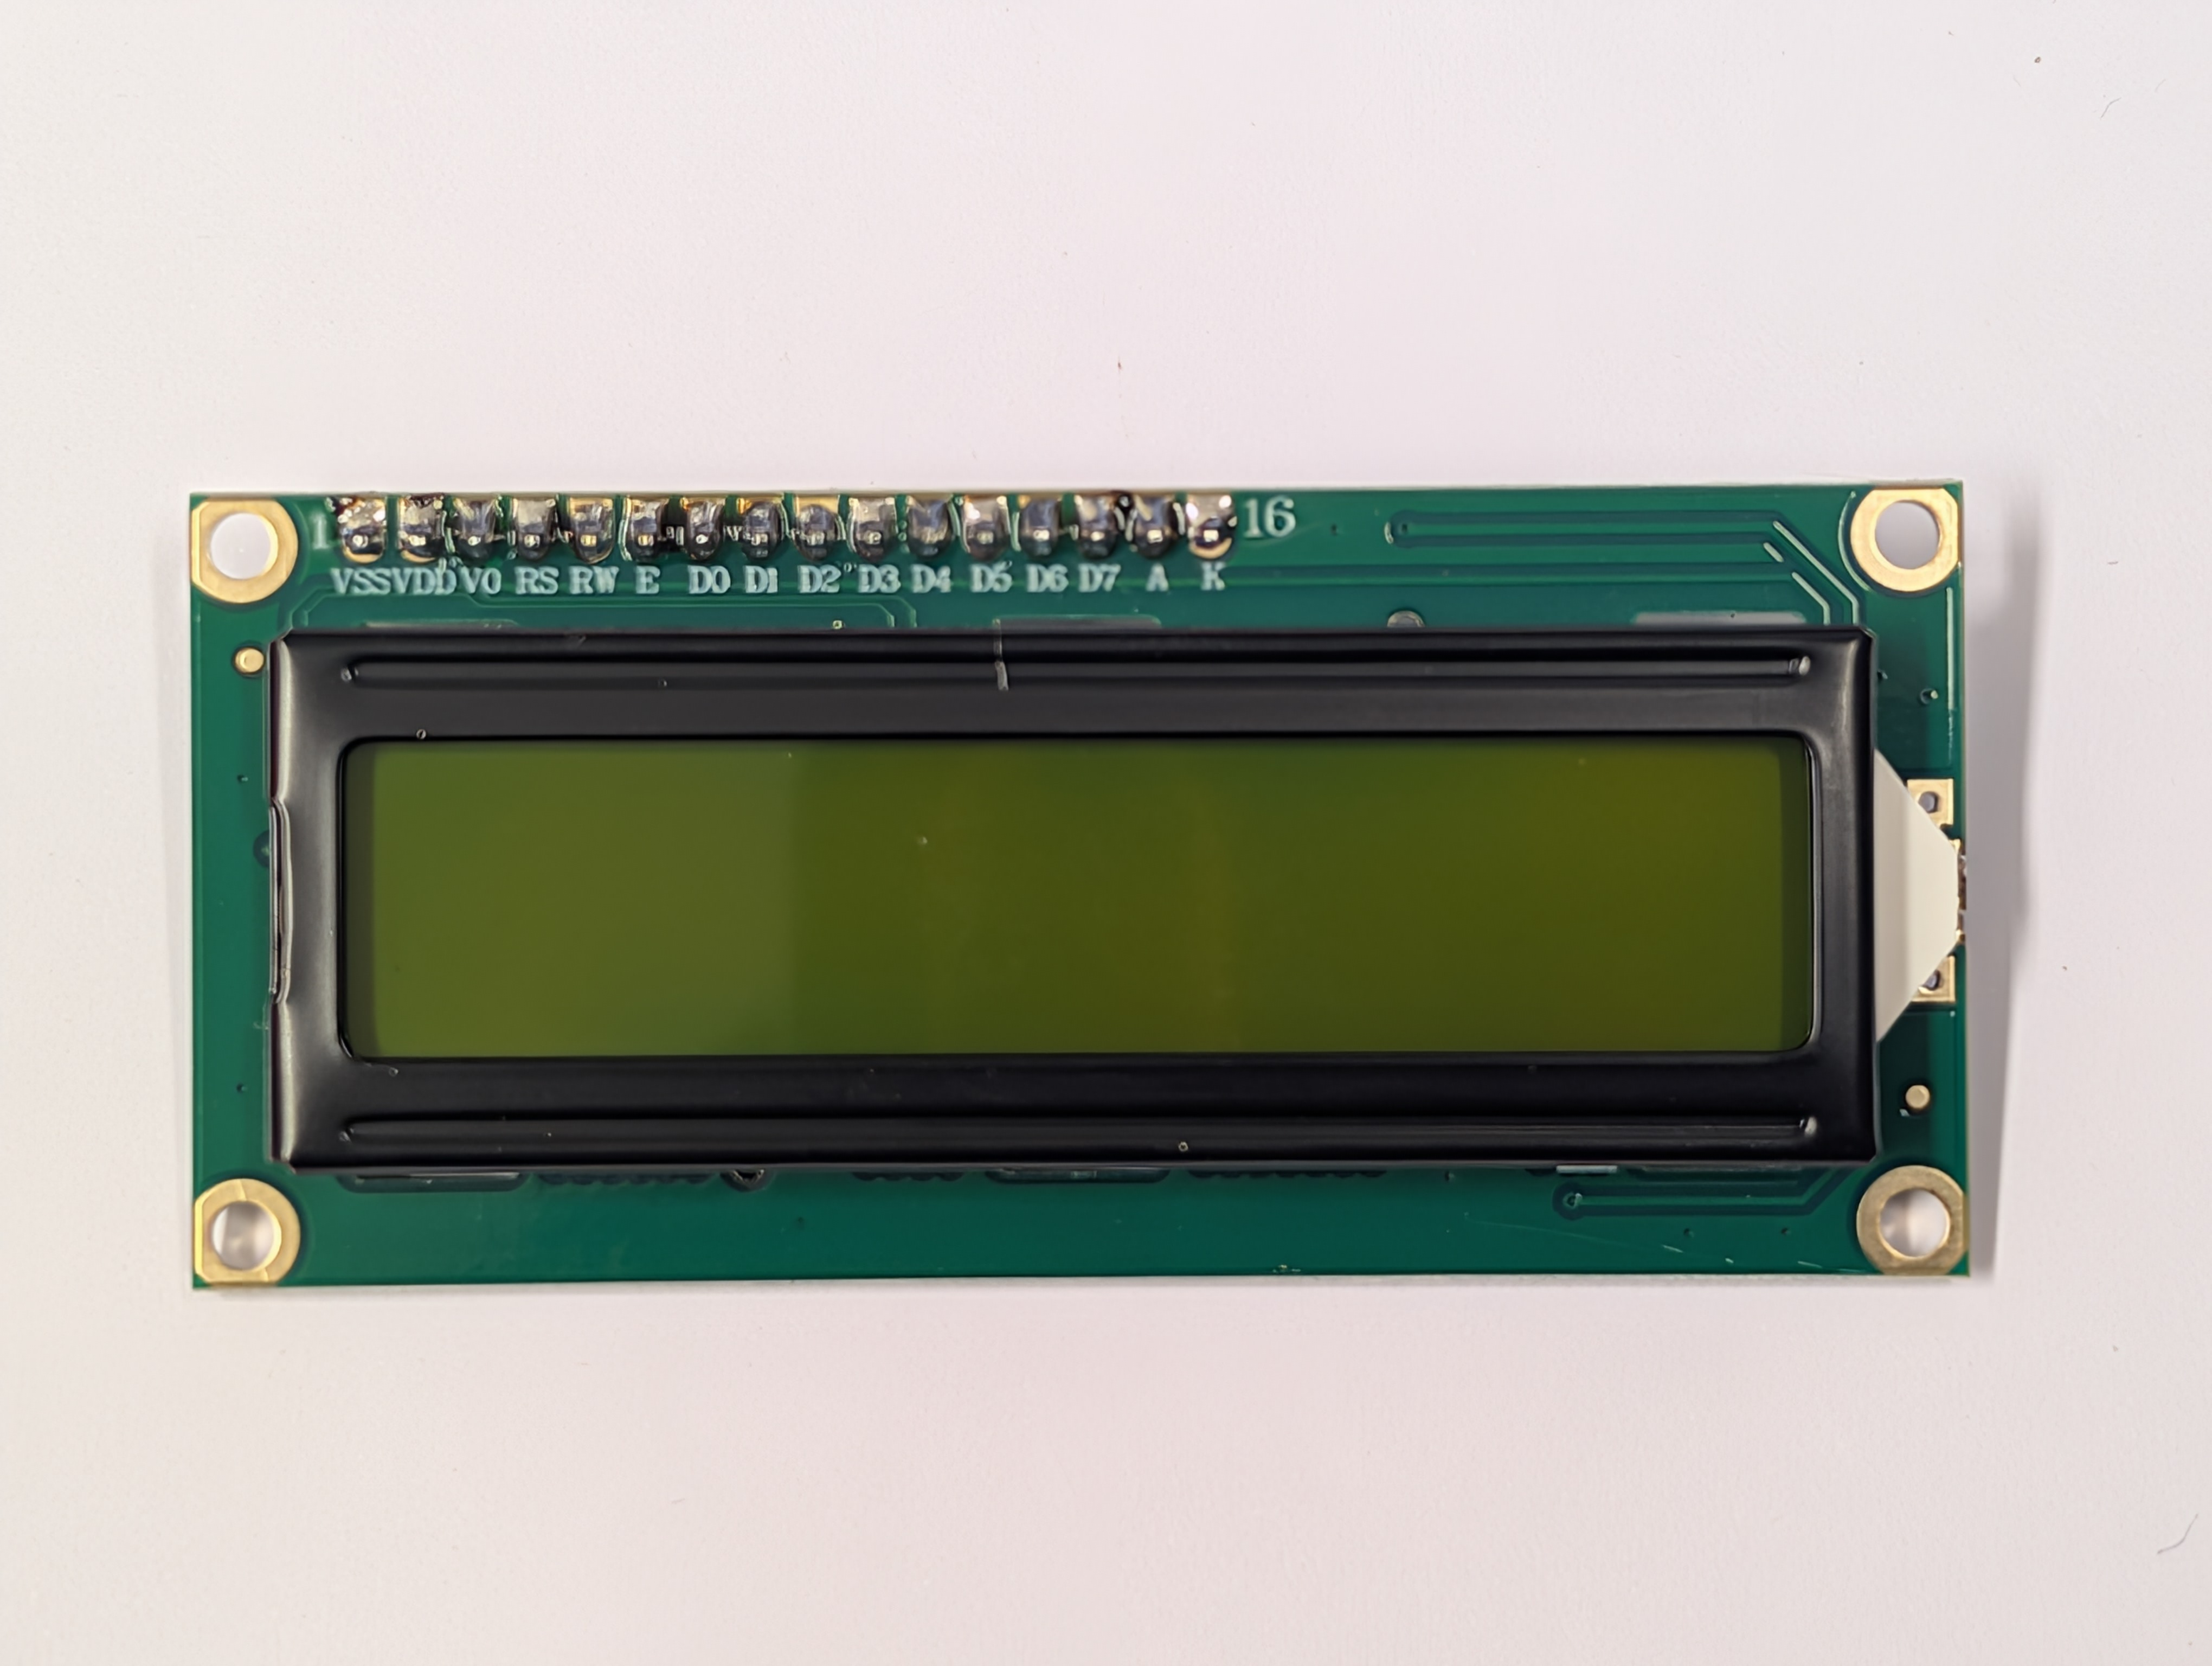
\includegraphics[width=0.75\textwidth]{pictures_of_construction/instruction_step_16.jpg}
\end{figure}

\subsection*{5. Widerstände einbauen}

Jetzt kommen die kleinen Widerstände auf die Platine.

\subsubsection*{Wichtig}
Die Drähte der Widerstände müssen vorher gebogen werden.

So geht’s:
\begin{enumerate}
    \item Biege die beiden Drahtenden vorsichtig nach unten, sodass eine U-Form entsteht.
    \item Stecke den Widerstand an die passende Stelle auf der Platine.
    \item Biege die Drähte auf der Rückseite leicht auseinander, damit er nicht herausfällt.
    \item Löte erst ein Bein fest.
    \item Prüfe, ob der Widerstand schön anliegt.
    \item Löte das zweite Bein.
    \item Schneide die überstehenden Drähte ab.
\end{enumerate}

\subsubsection*{5a. NTC-Widerstand einbauen}

Der NTC ist ein besonderer Temperaturwiderstand.

Merkmal:
\begin{itemize}
    \item Er hat ein \textbf{Glasgehäuse}
    \item Er hat \textbf{keine Farbringe}
\end{itemize}

Stecke ihn an die Stelle \textbf{TH\_NTC}.

\textbf{Wichtig:}
\begin{itemize}
    \item Die \textbf{bedruckte Seite} der Platine ist die Vorderseite.
    \item Unten links sollte das \textbf{DIGITEC-Logo} zu sehen sein.
\end{itemize}

\begin{figure}[H]
    \centering
    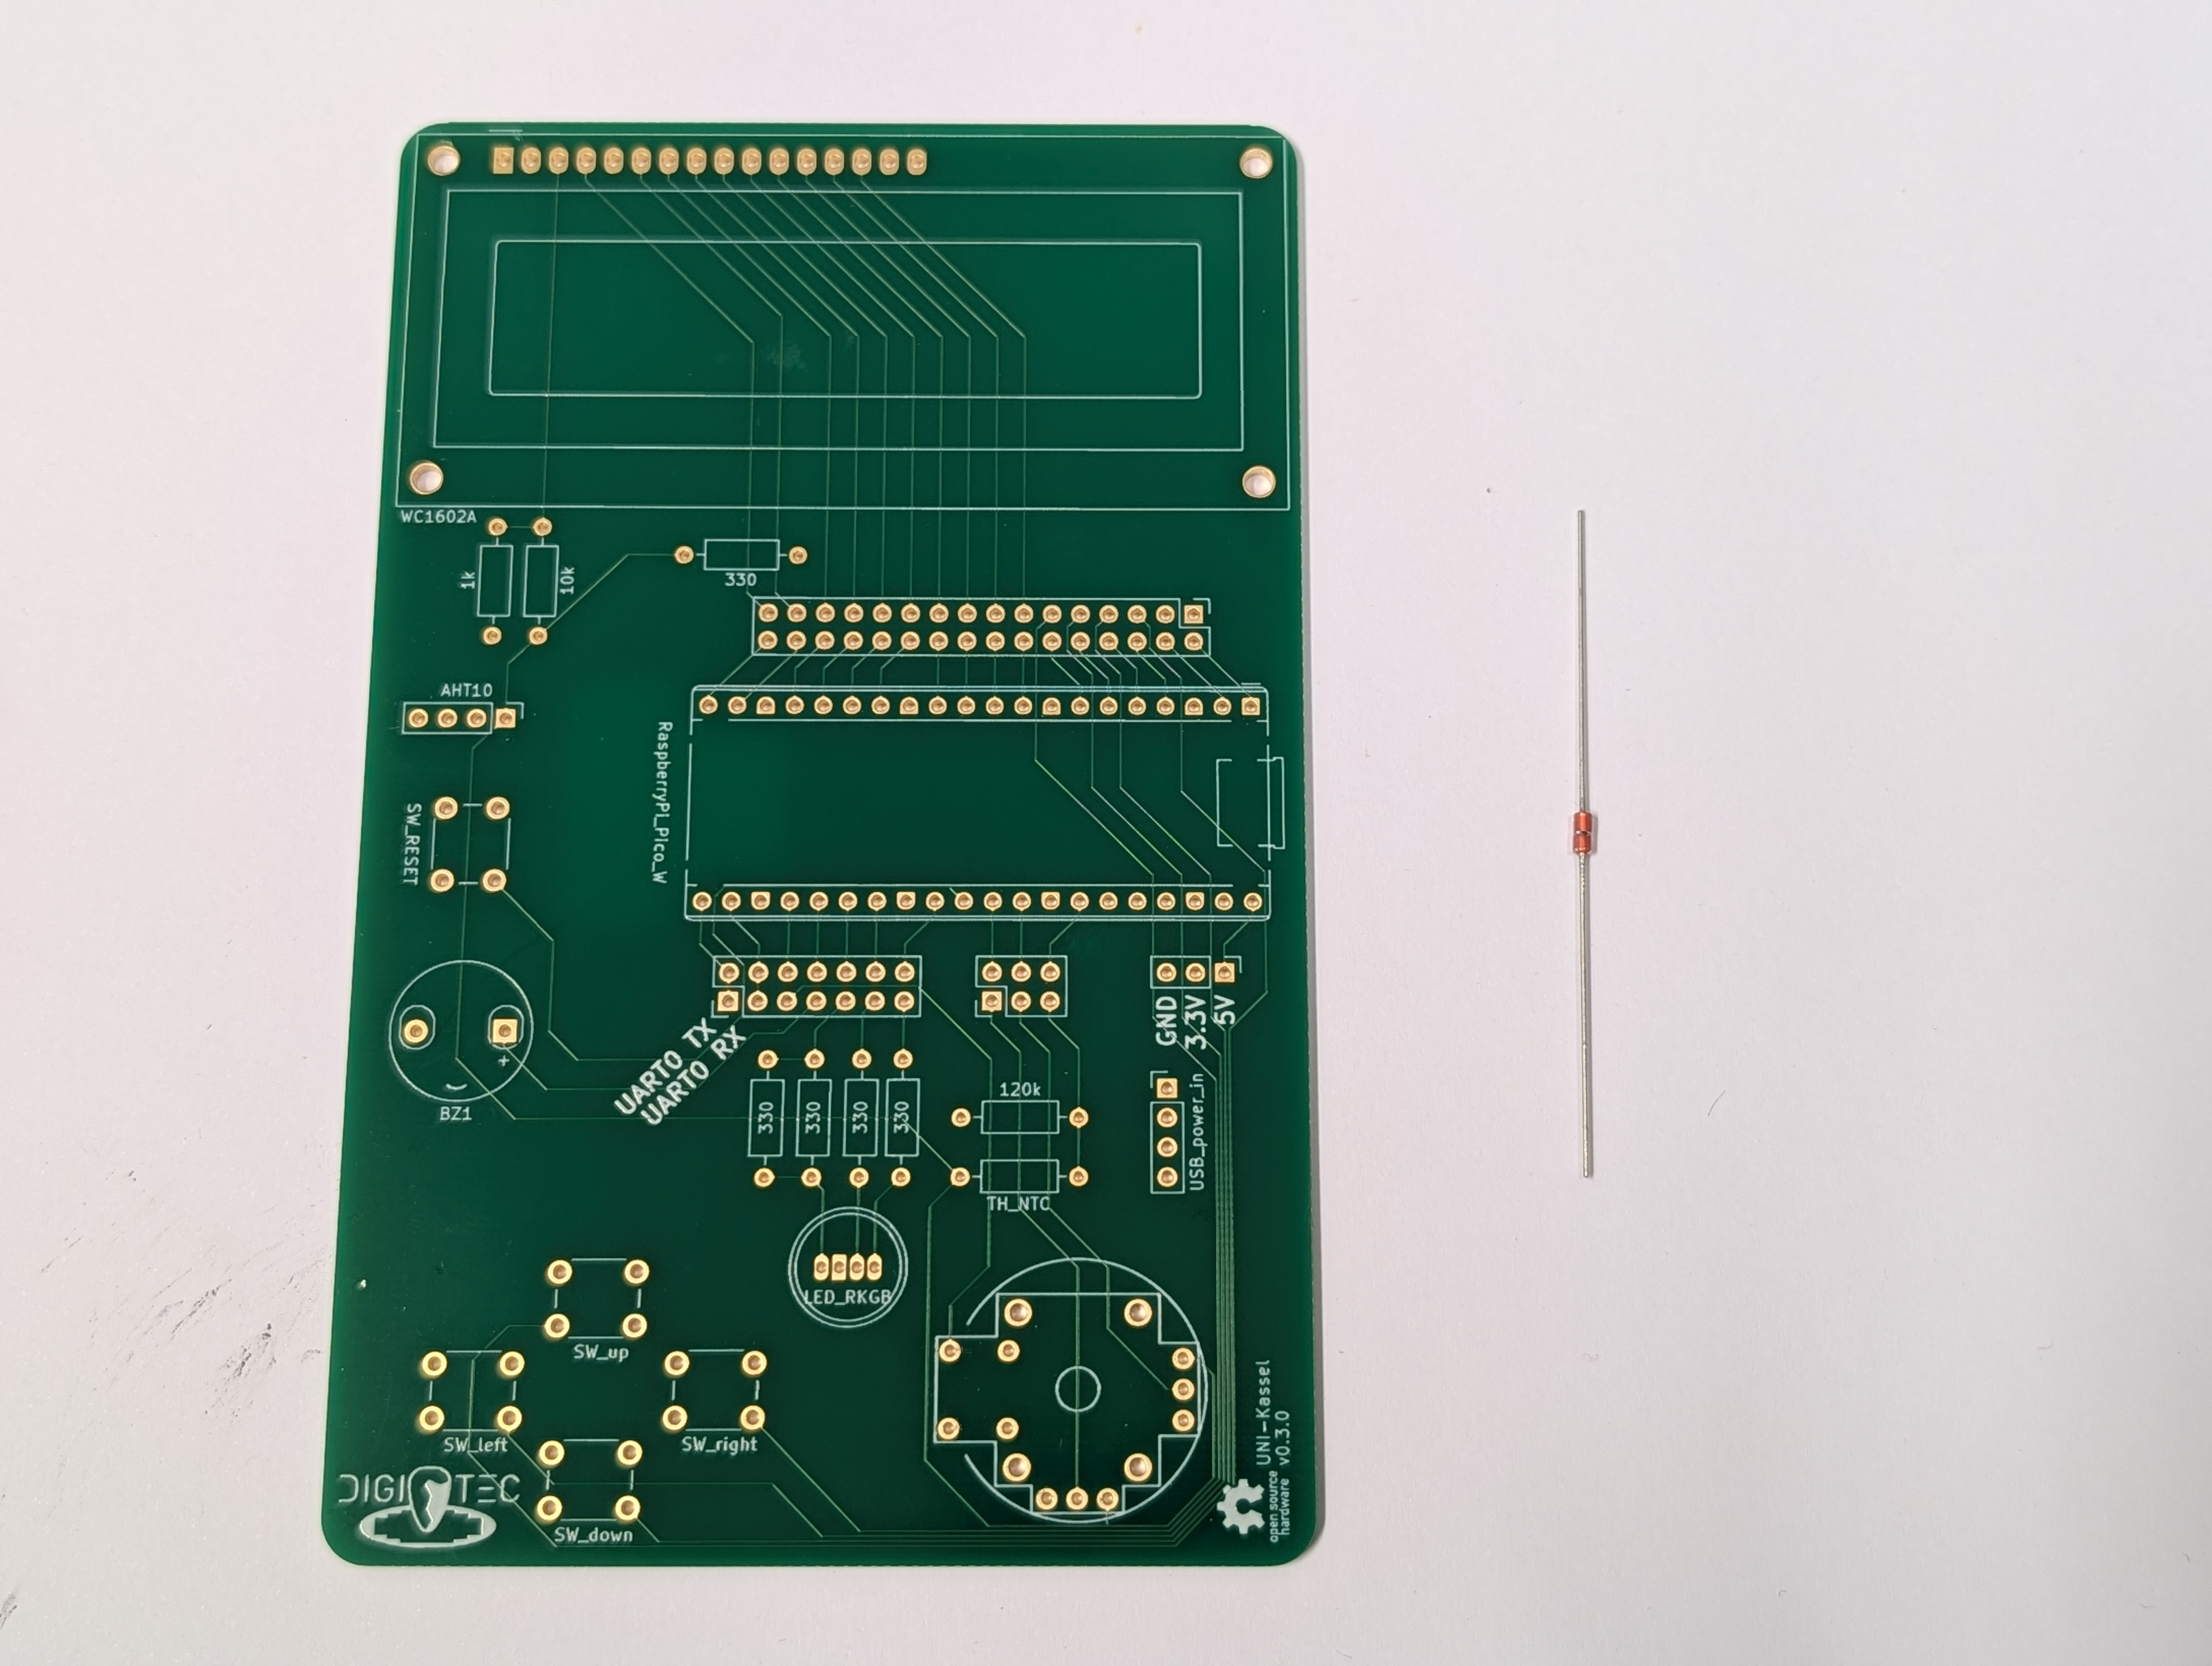
\includegraphics[width=0.75\textwidth]{pictures_of_construction/instruction_step_17.jpg}
\end{figure}

\begin{figure}[H]
    \centering
    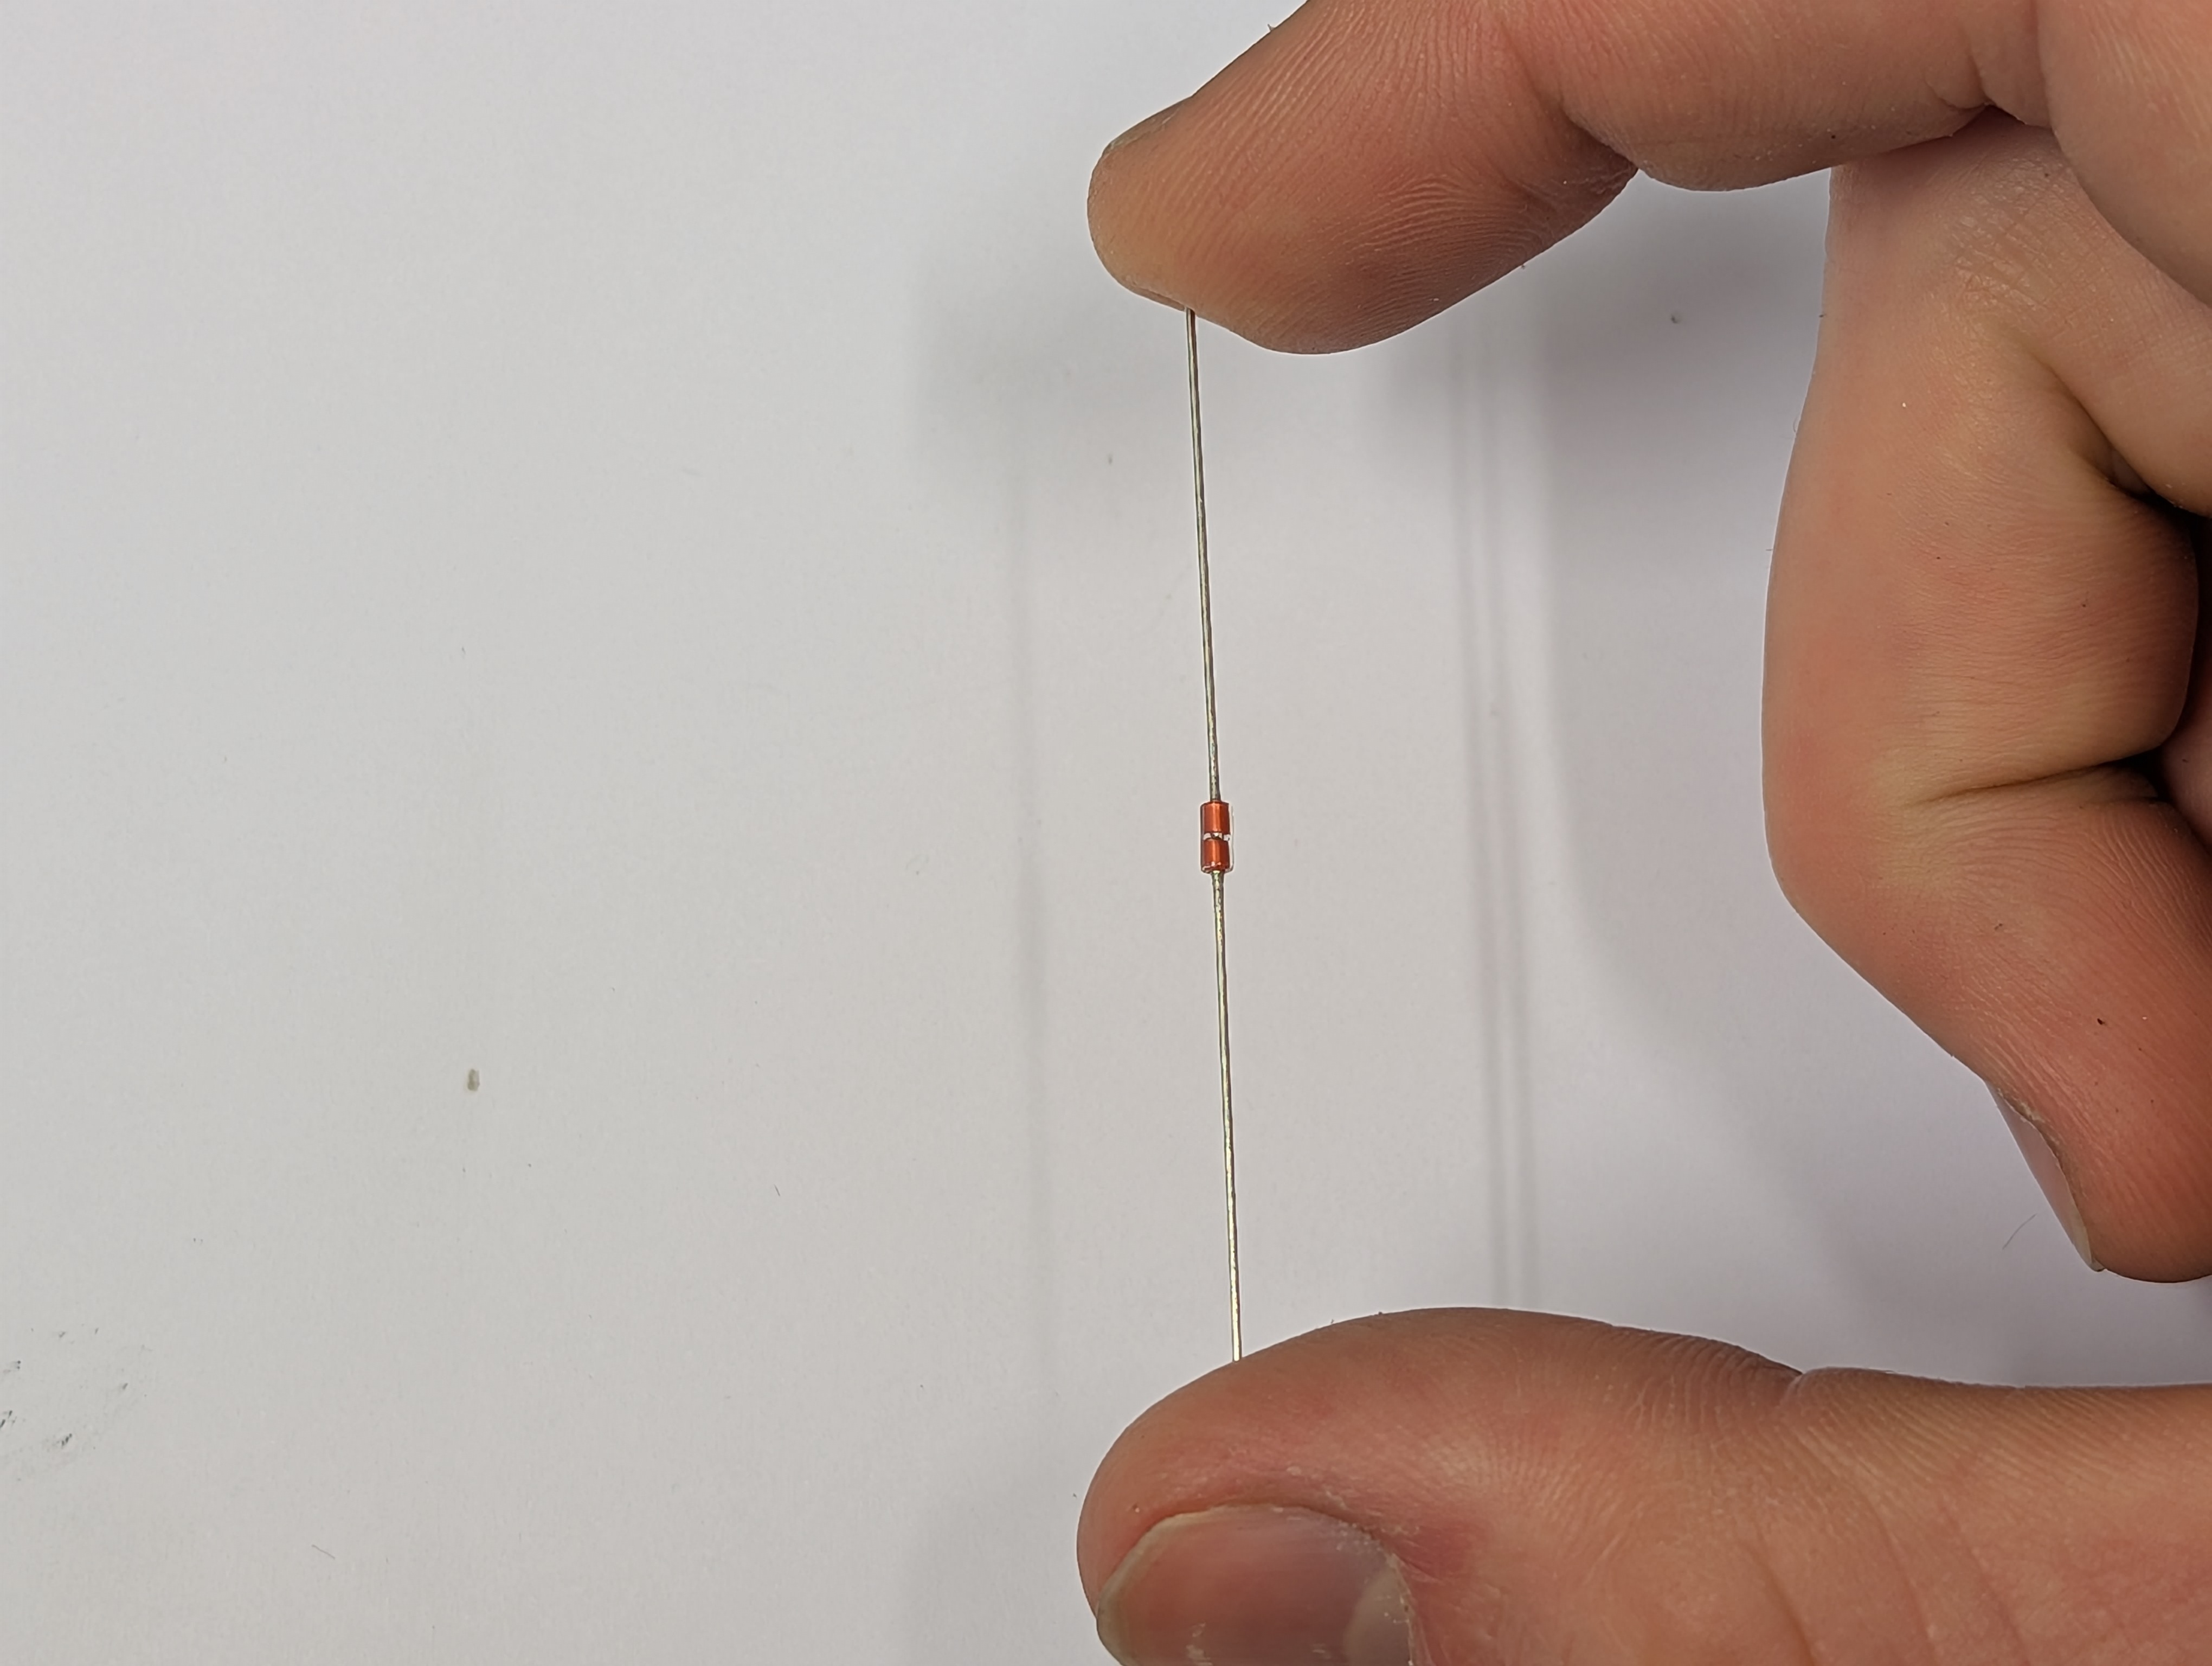
\includegraphics[width=0.75\textwidth]{pictures_of_construction/instruction_step_18.jpg}
\end{figure}

\begin{figure}[H]
    \centering
    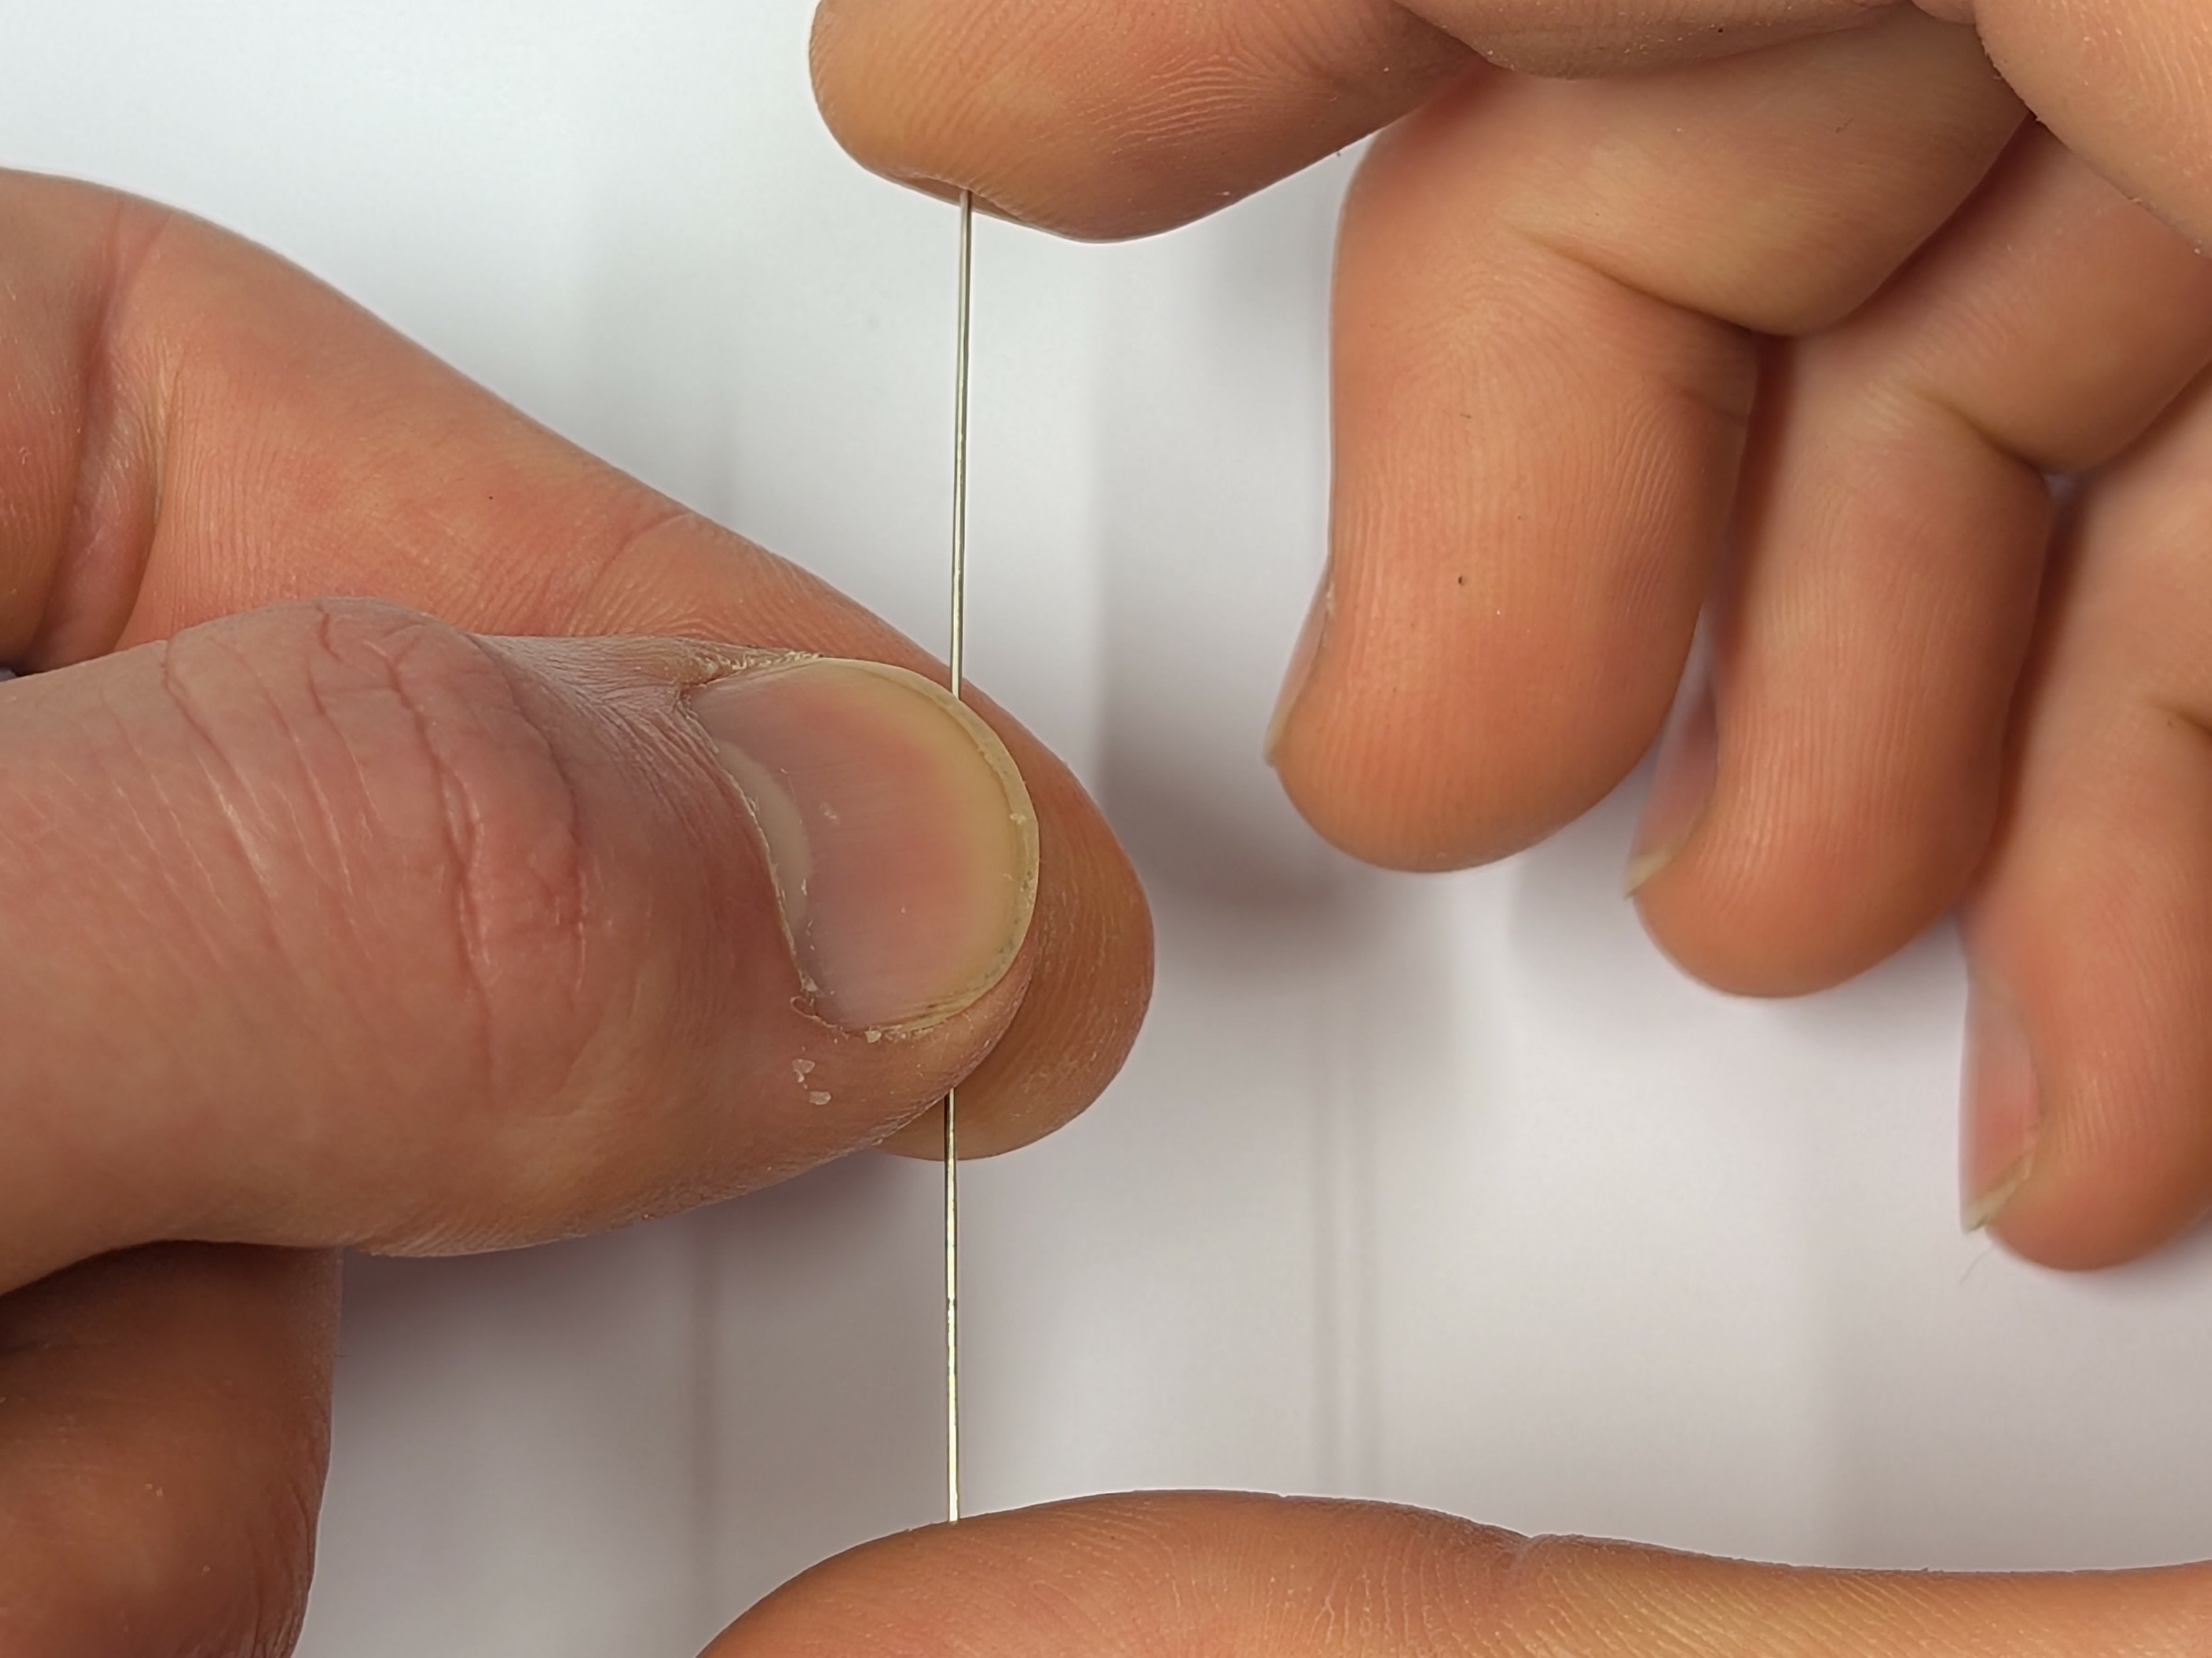
\includegraphics[width=0.75\textwidth]{pictures_of_construction/instruction_step_19.jpg}
\end{figure}

\begin{figure}[H]
    \centering
    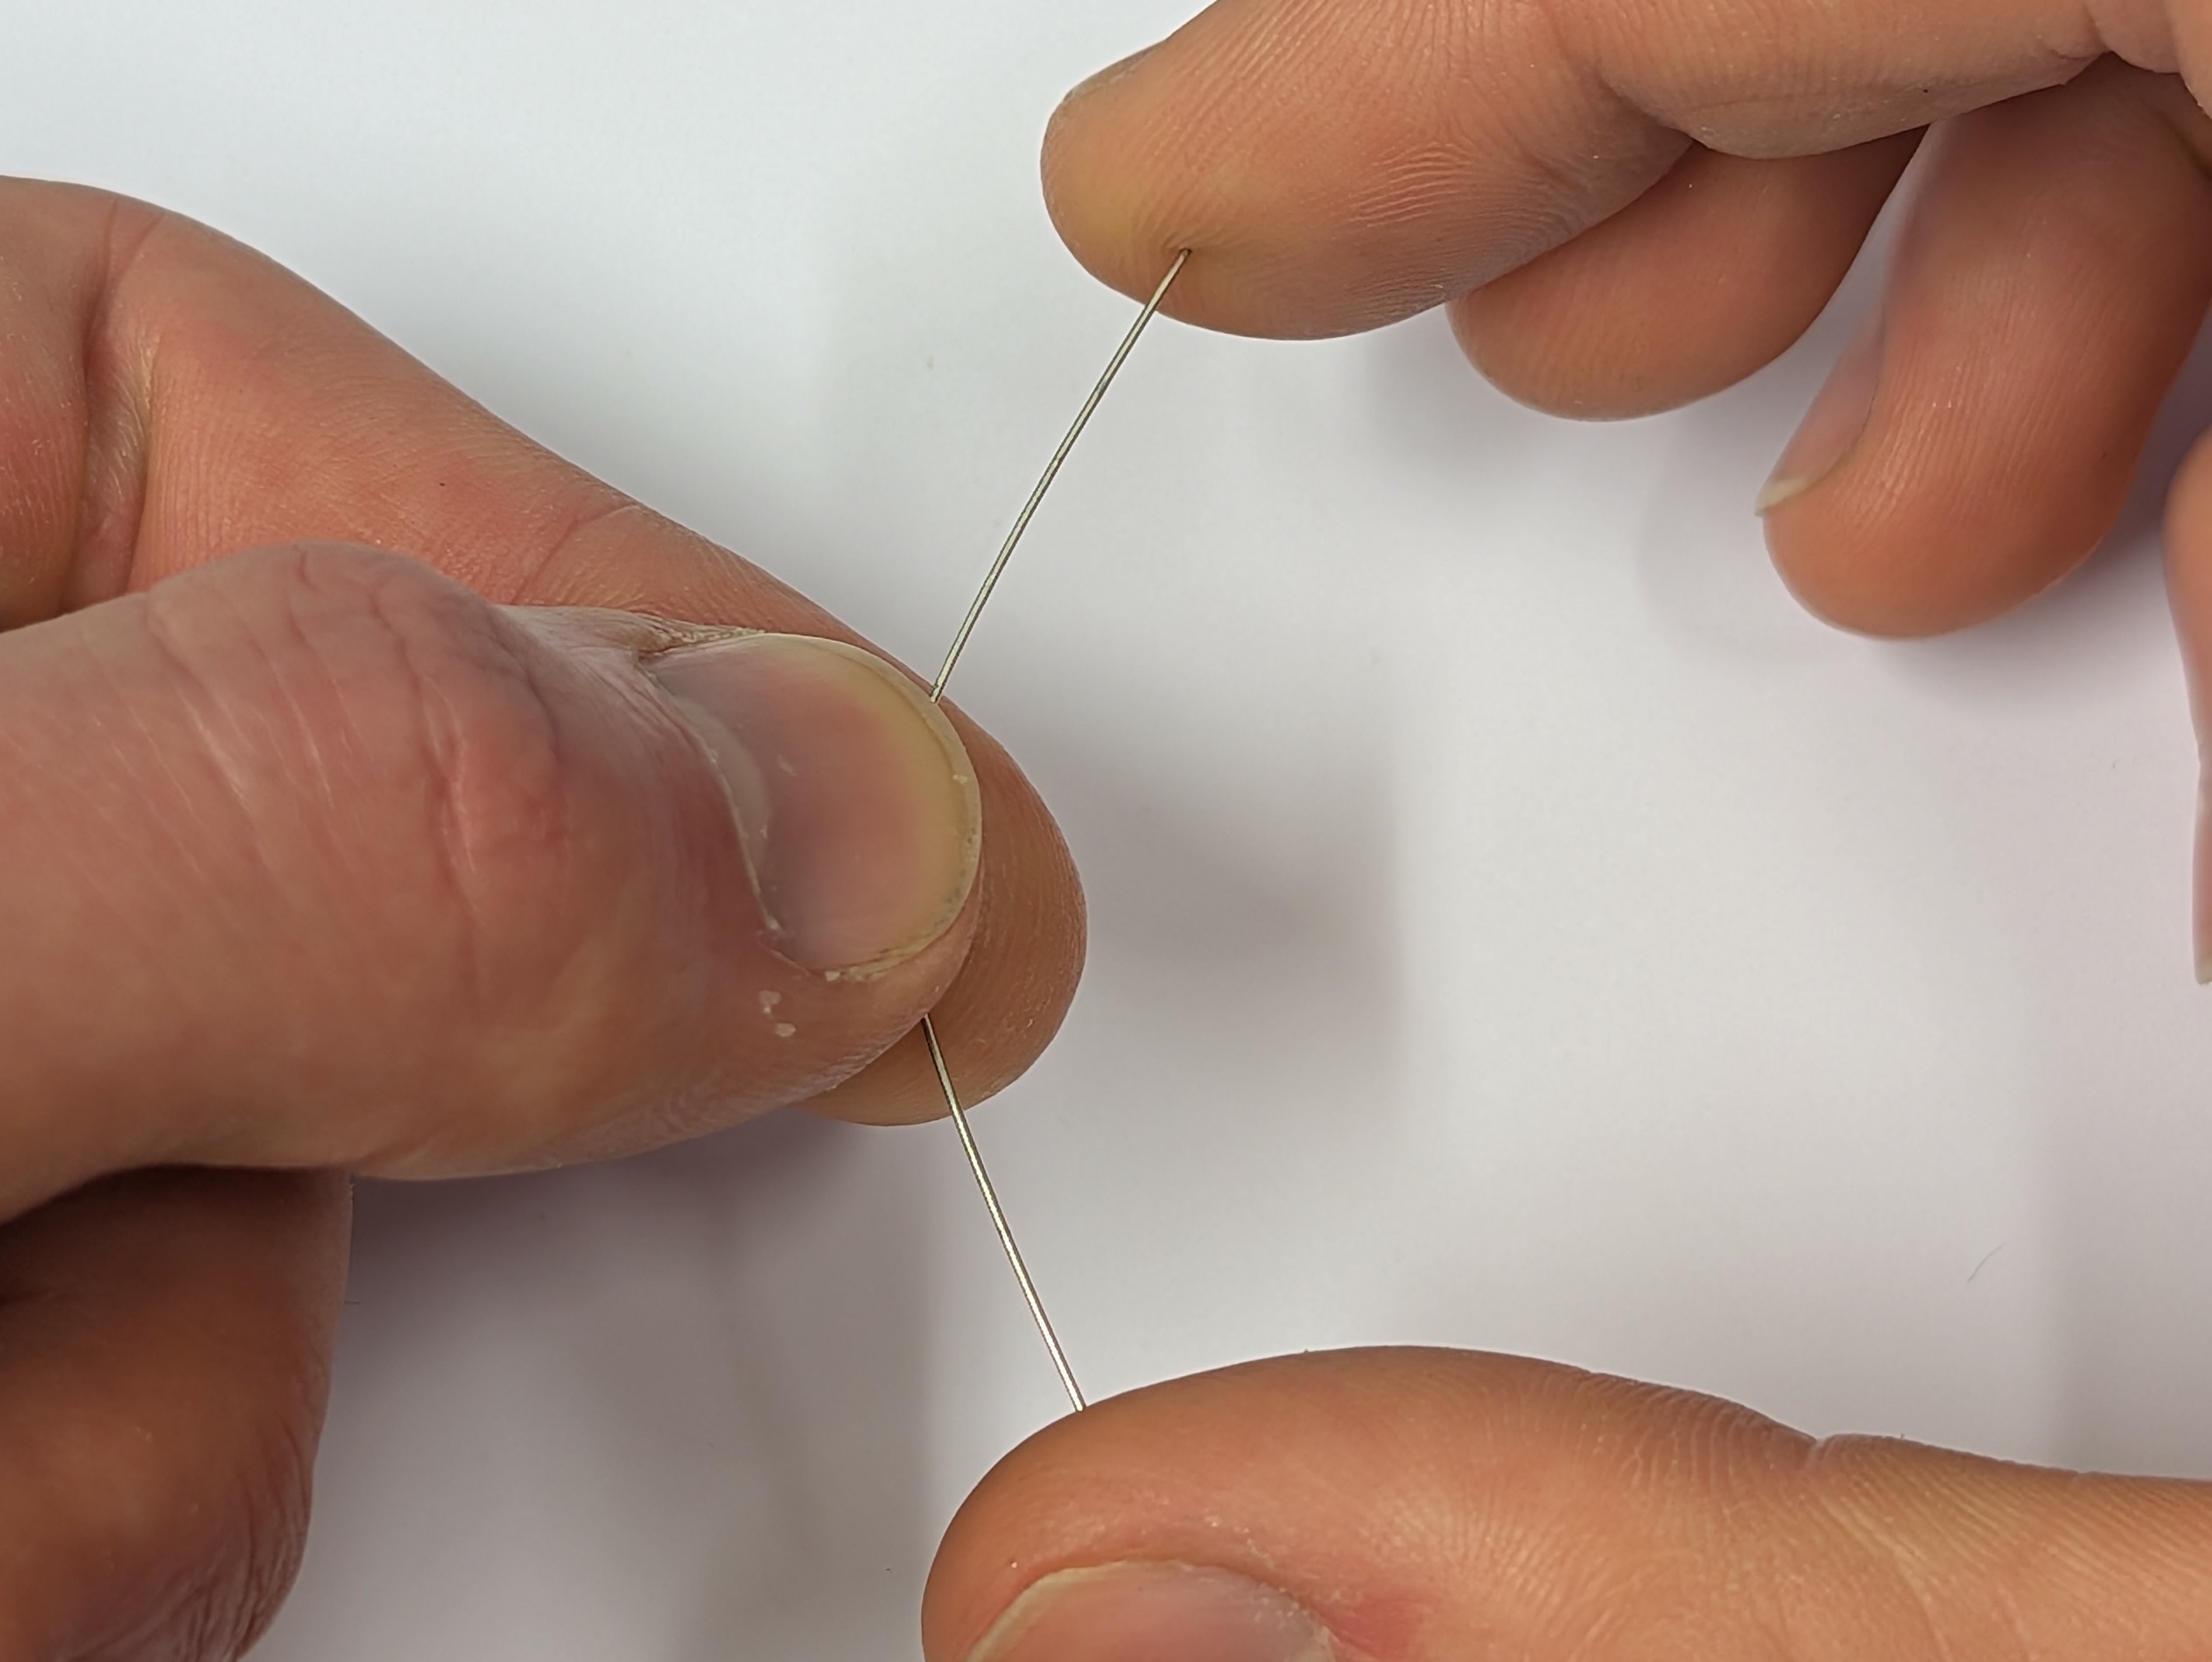
\includegraphics[width=0.75\textwidth]{pictures_of_construction/instruction_step_20.jpg}
\end{figure}

\begin{figure}[H]
    \centering
    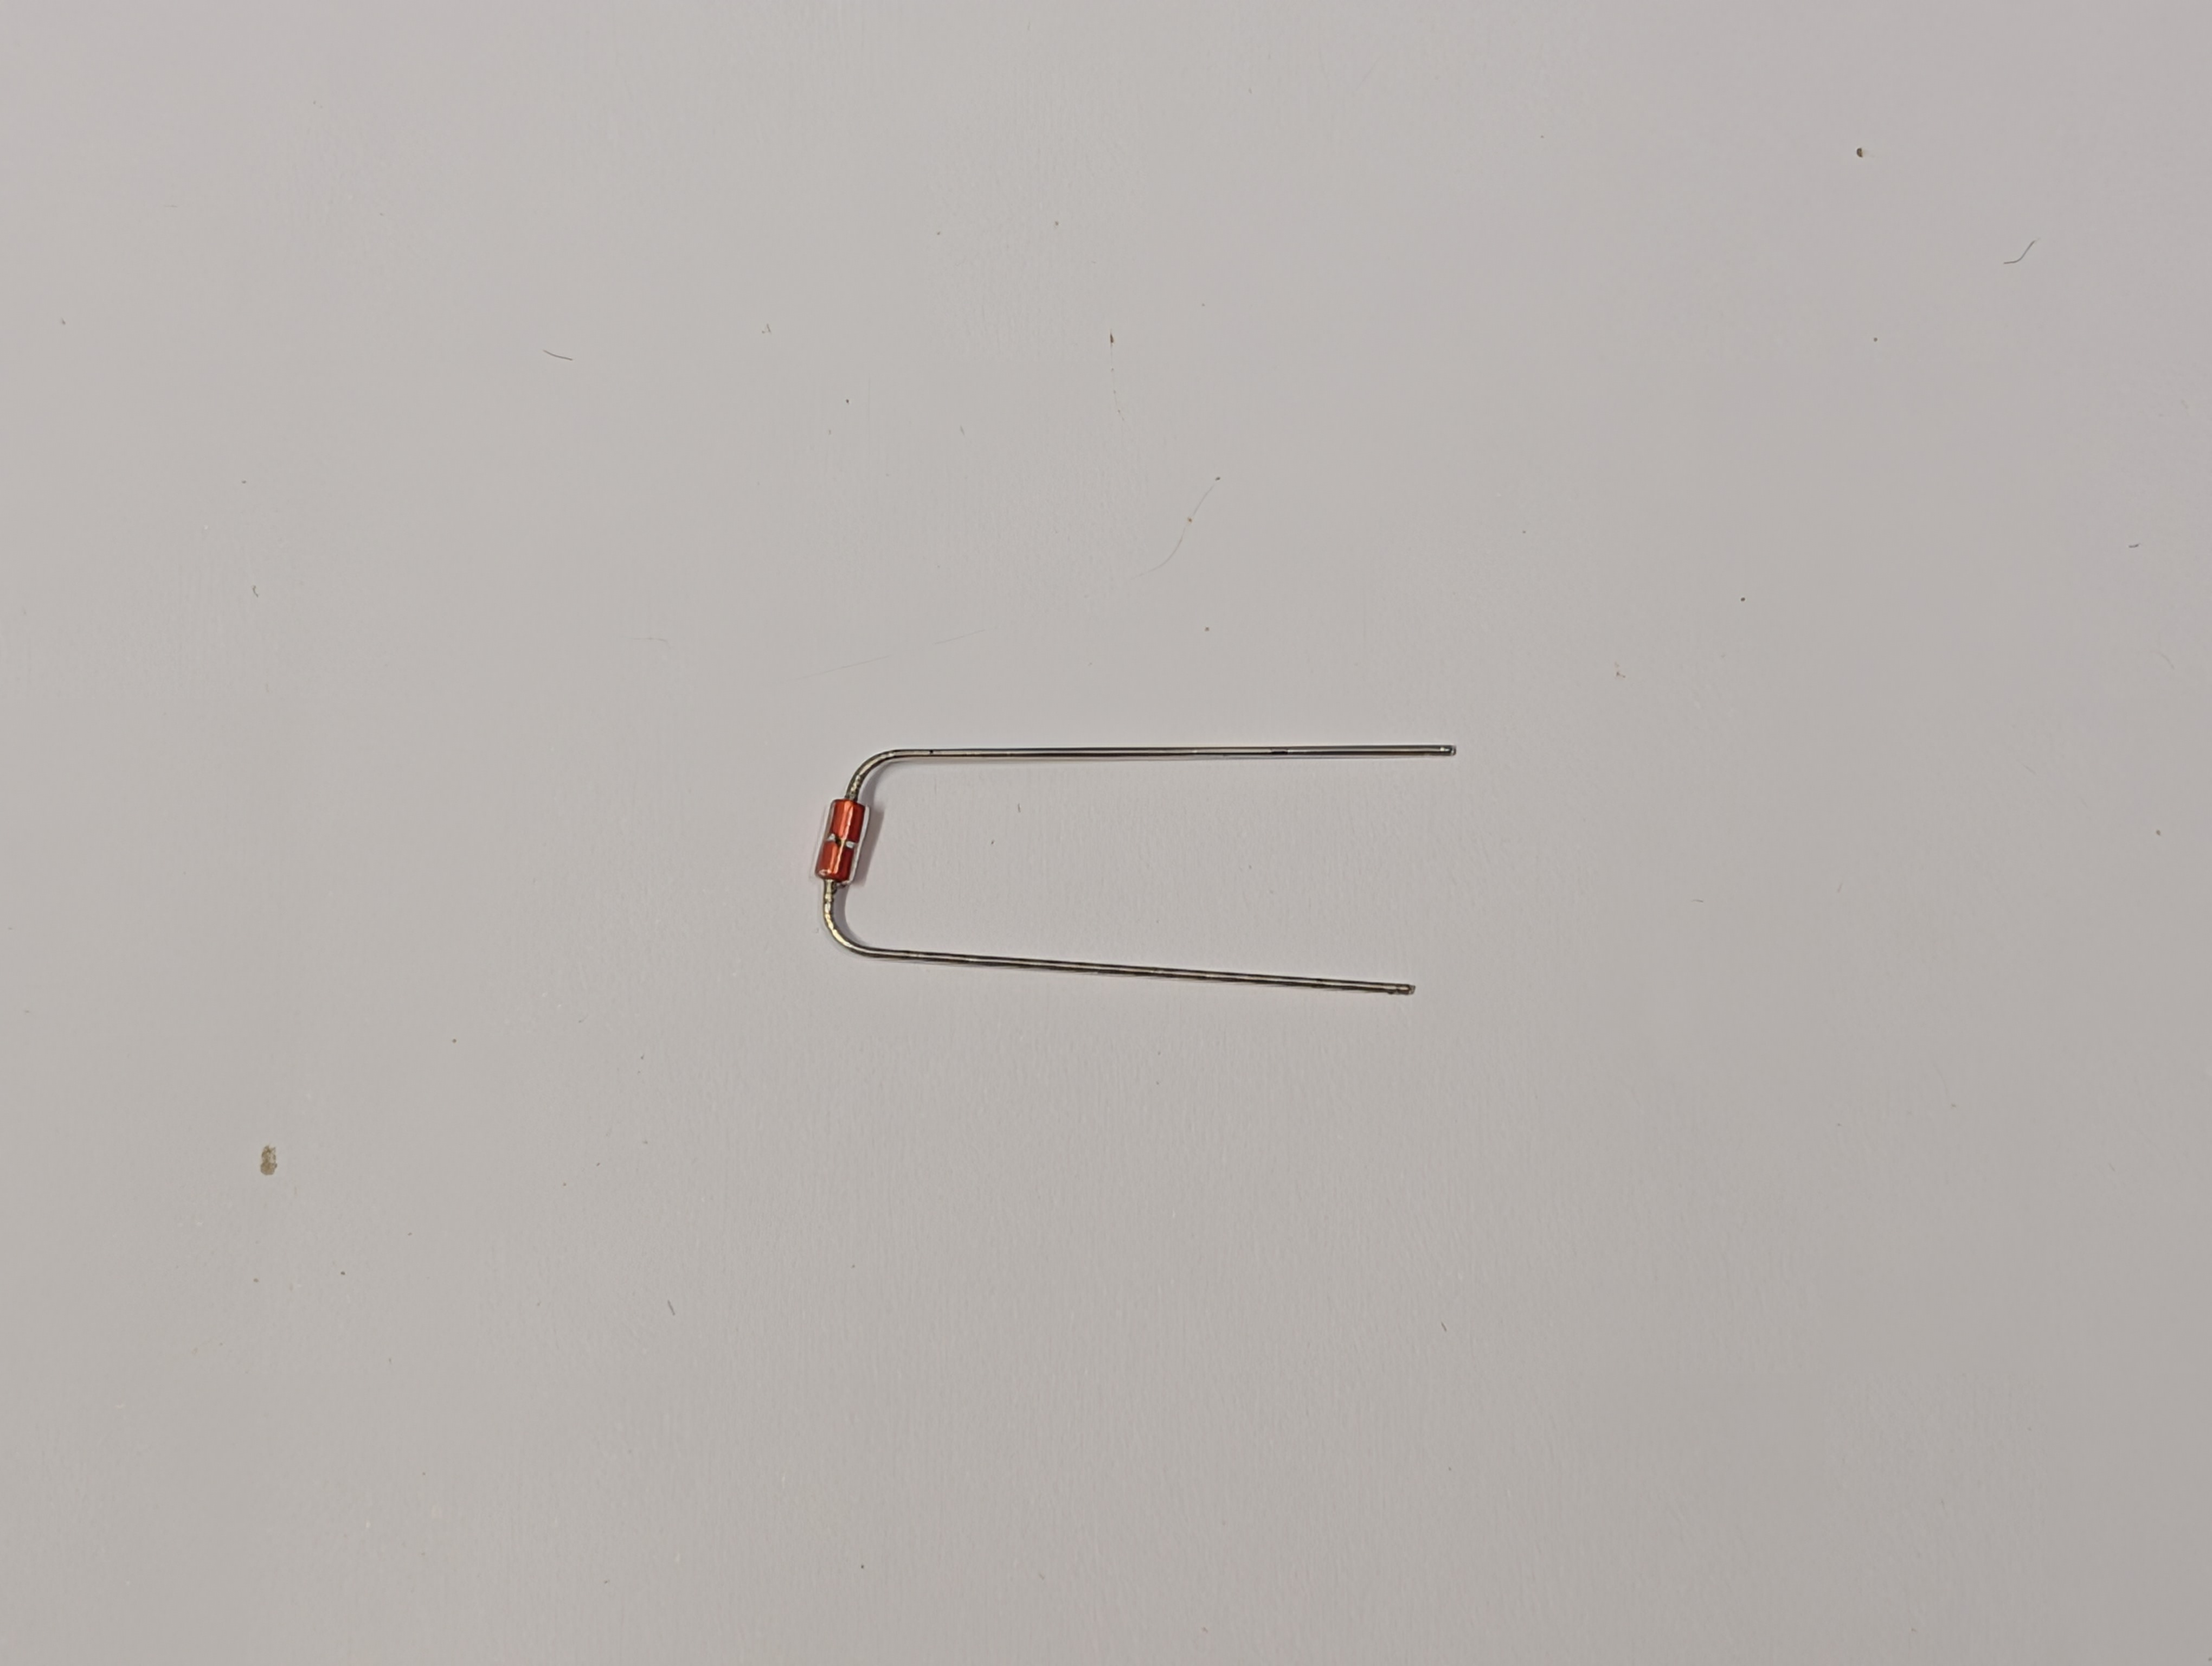
\includegraphics[width=0.75\textwidth]{pictures_of_construction/instruction_step_21.jpg}
\end{figure}

\begin{figure}[H]
    \centering
    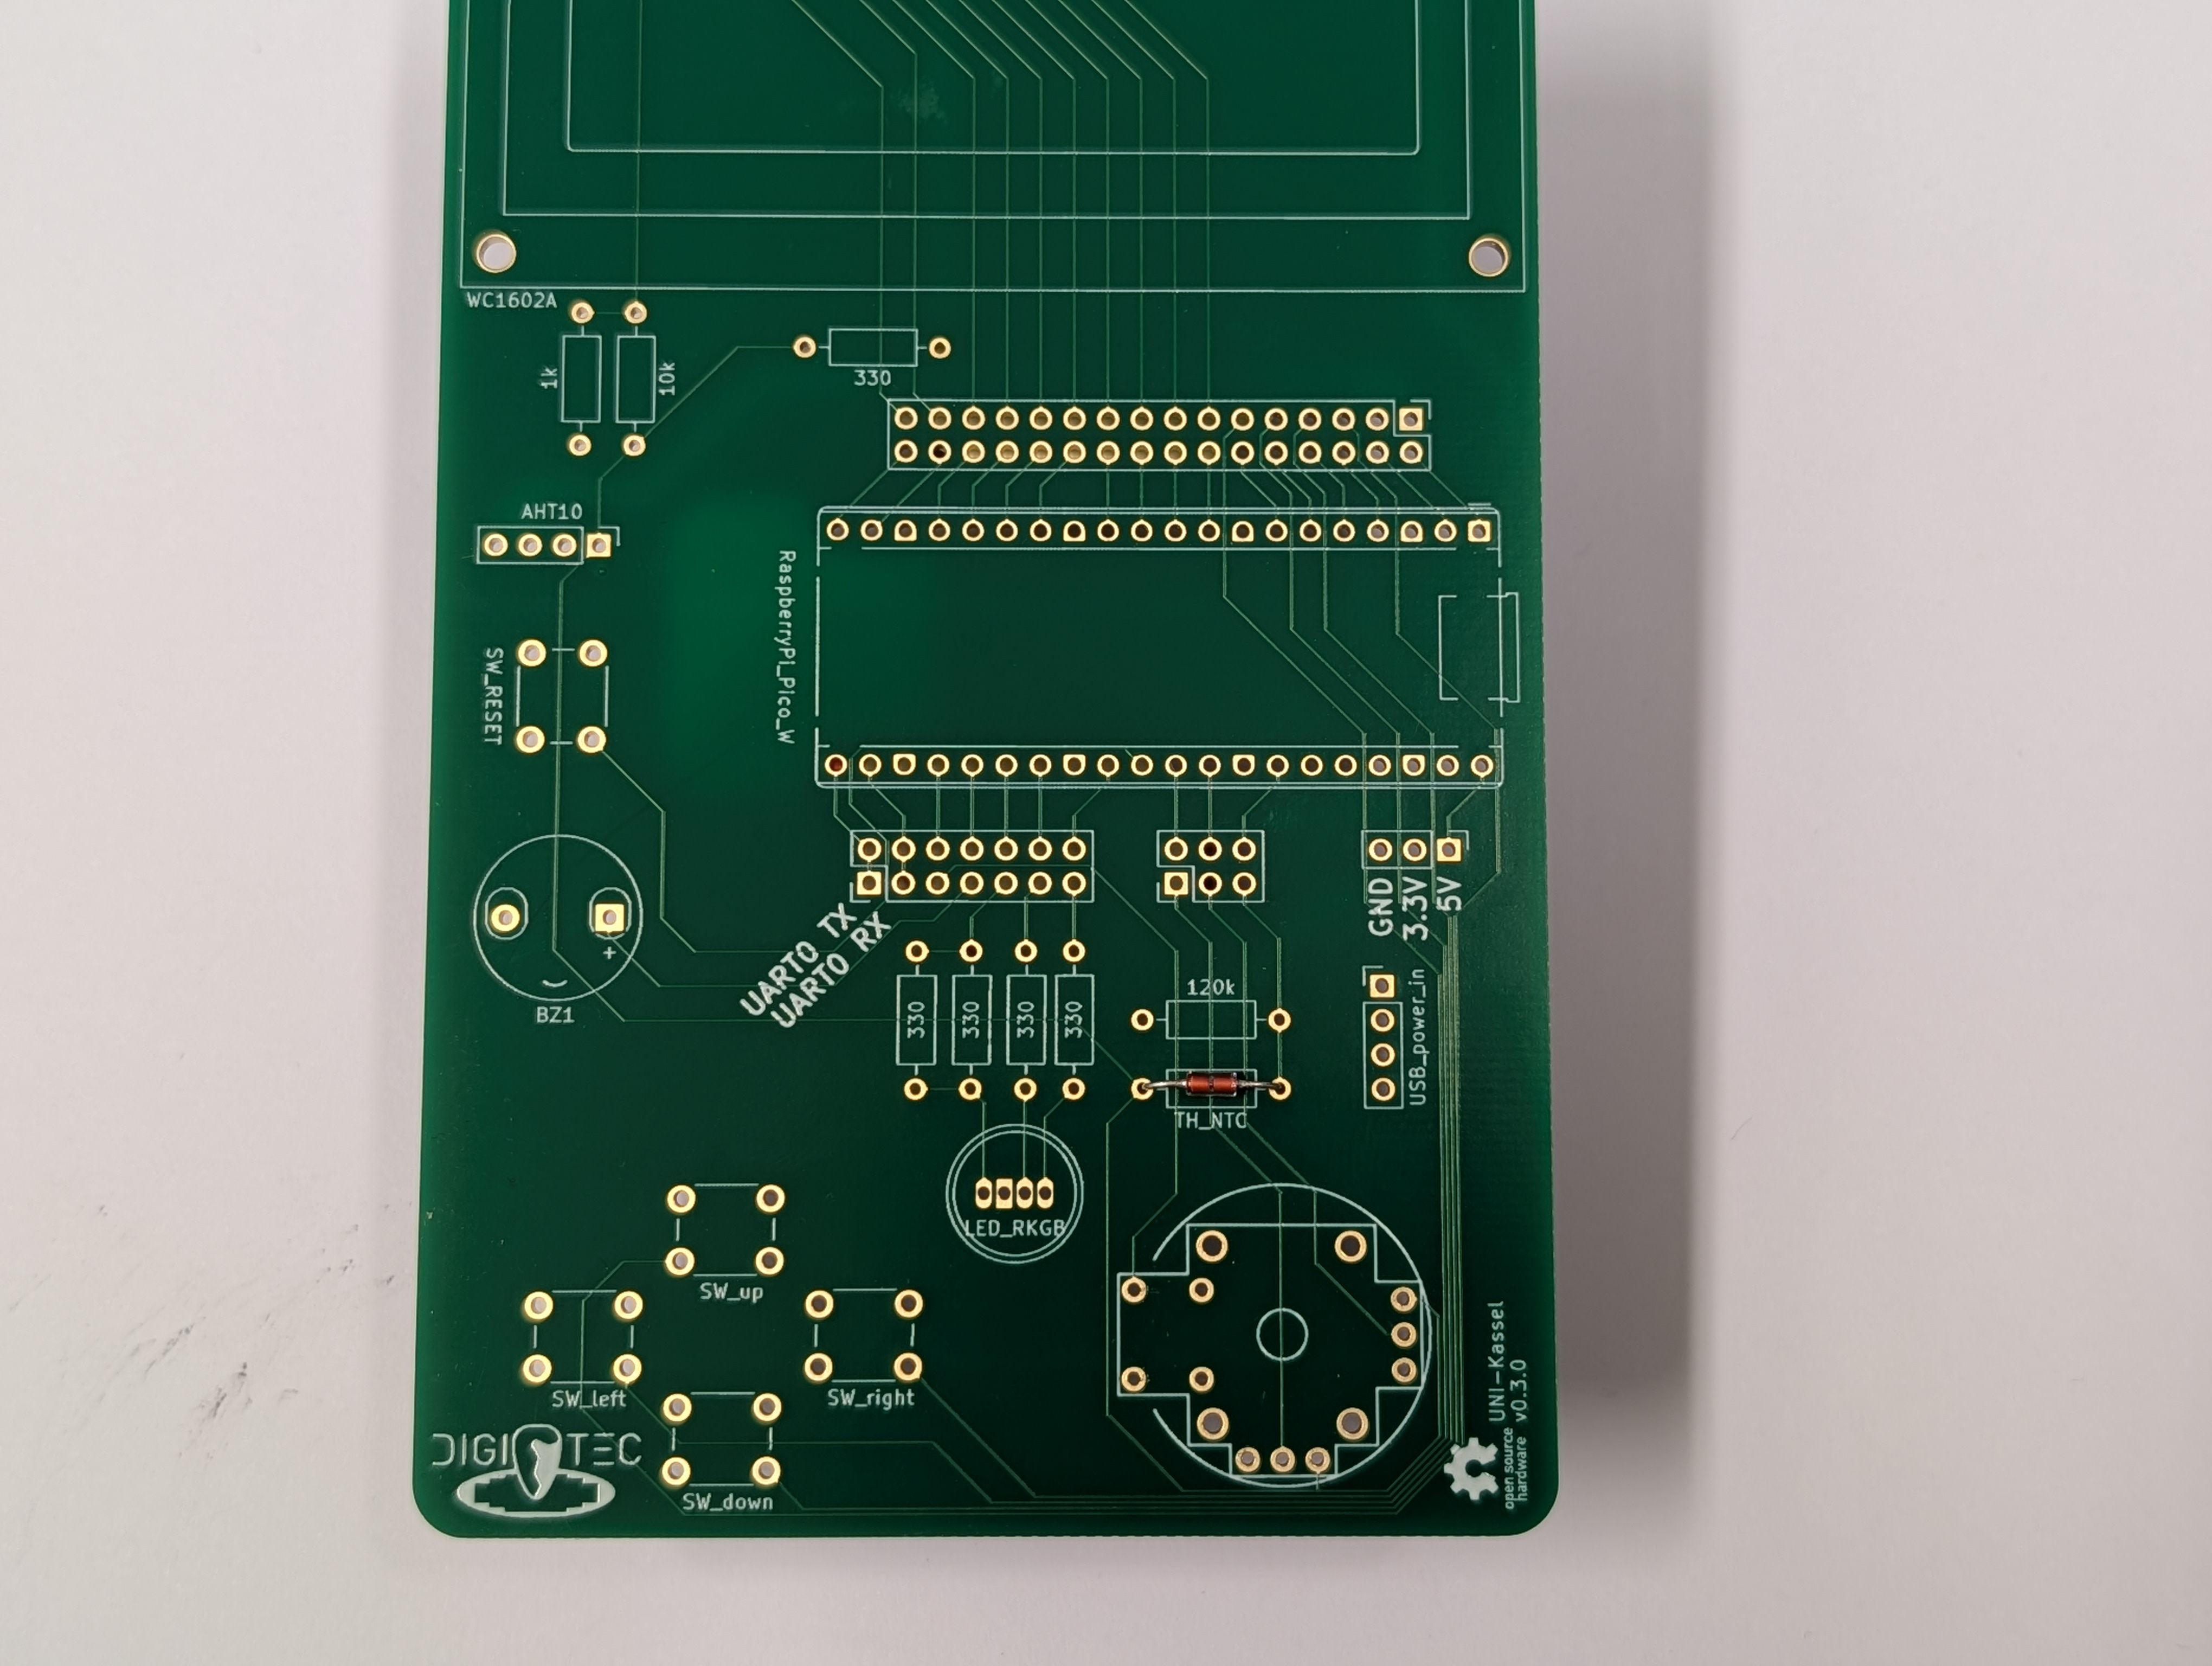
\includegraphics[width=0.75\textwidth]{pictures_of_construction/instruction_step_22.jpg}
\end{figure}

\begin{figure}[H]
    \centering
    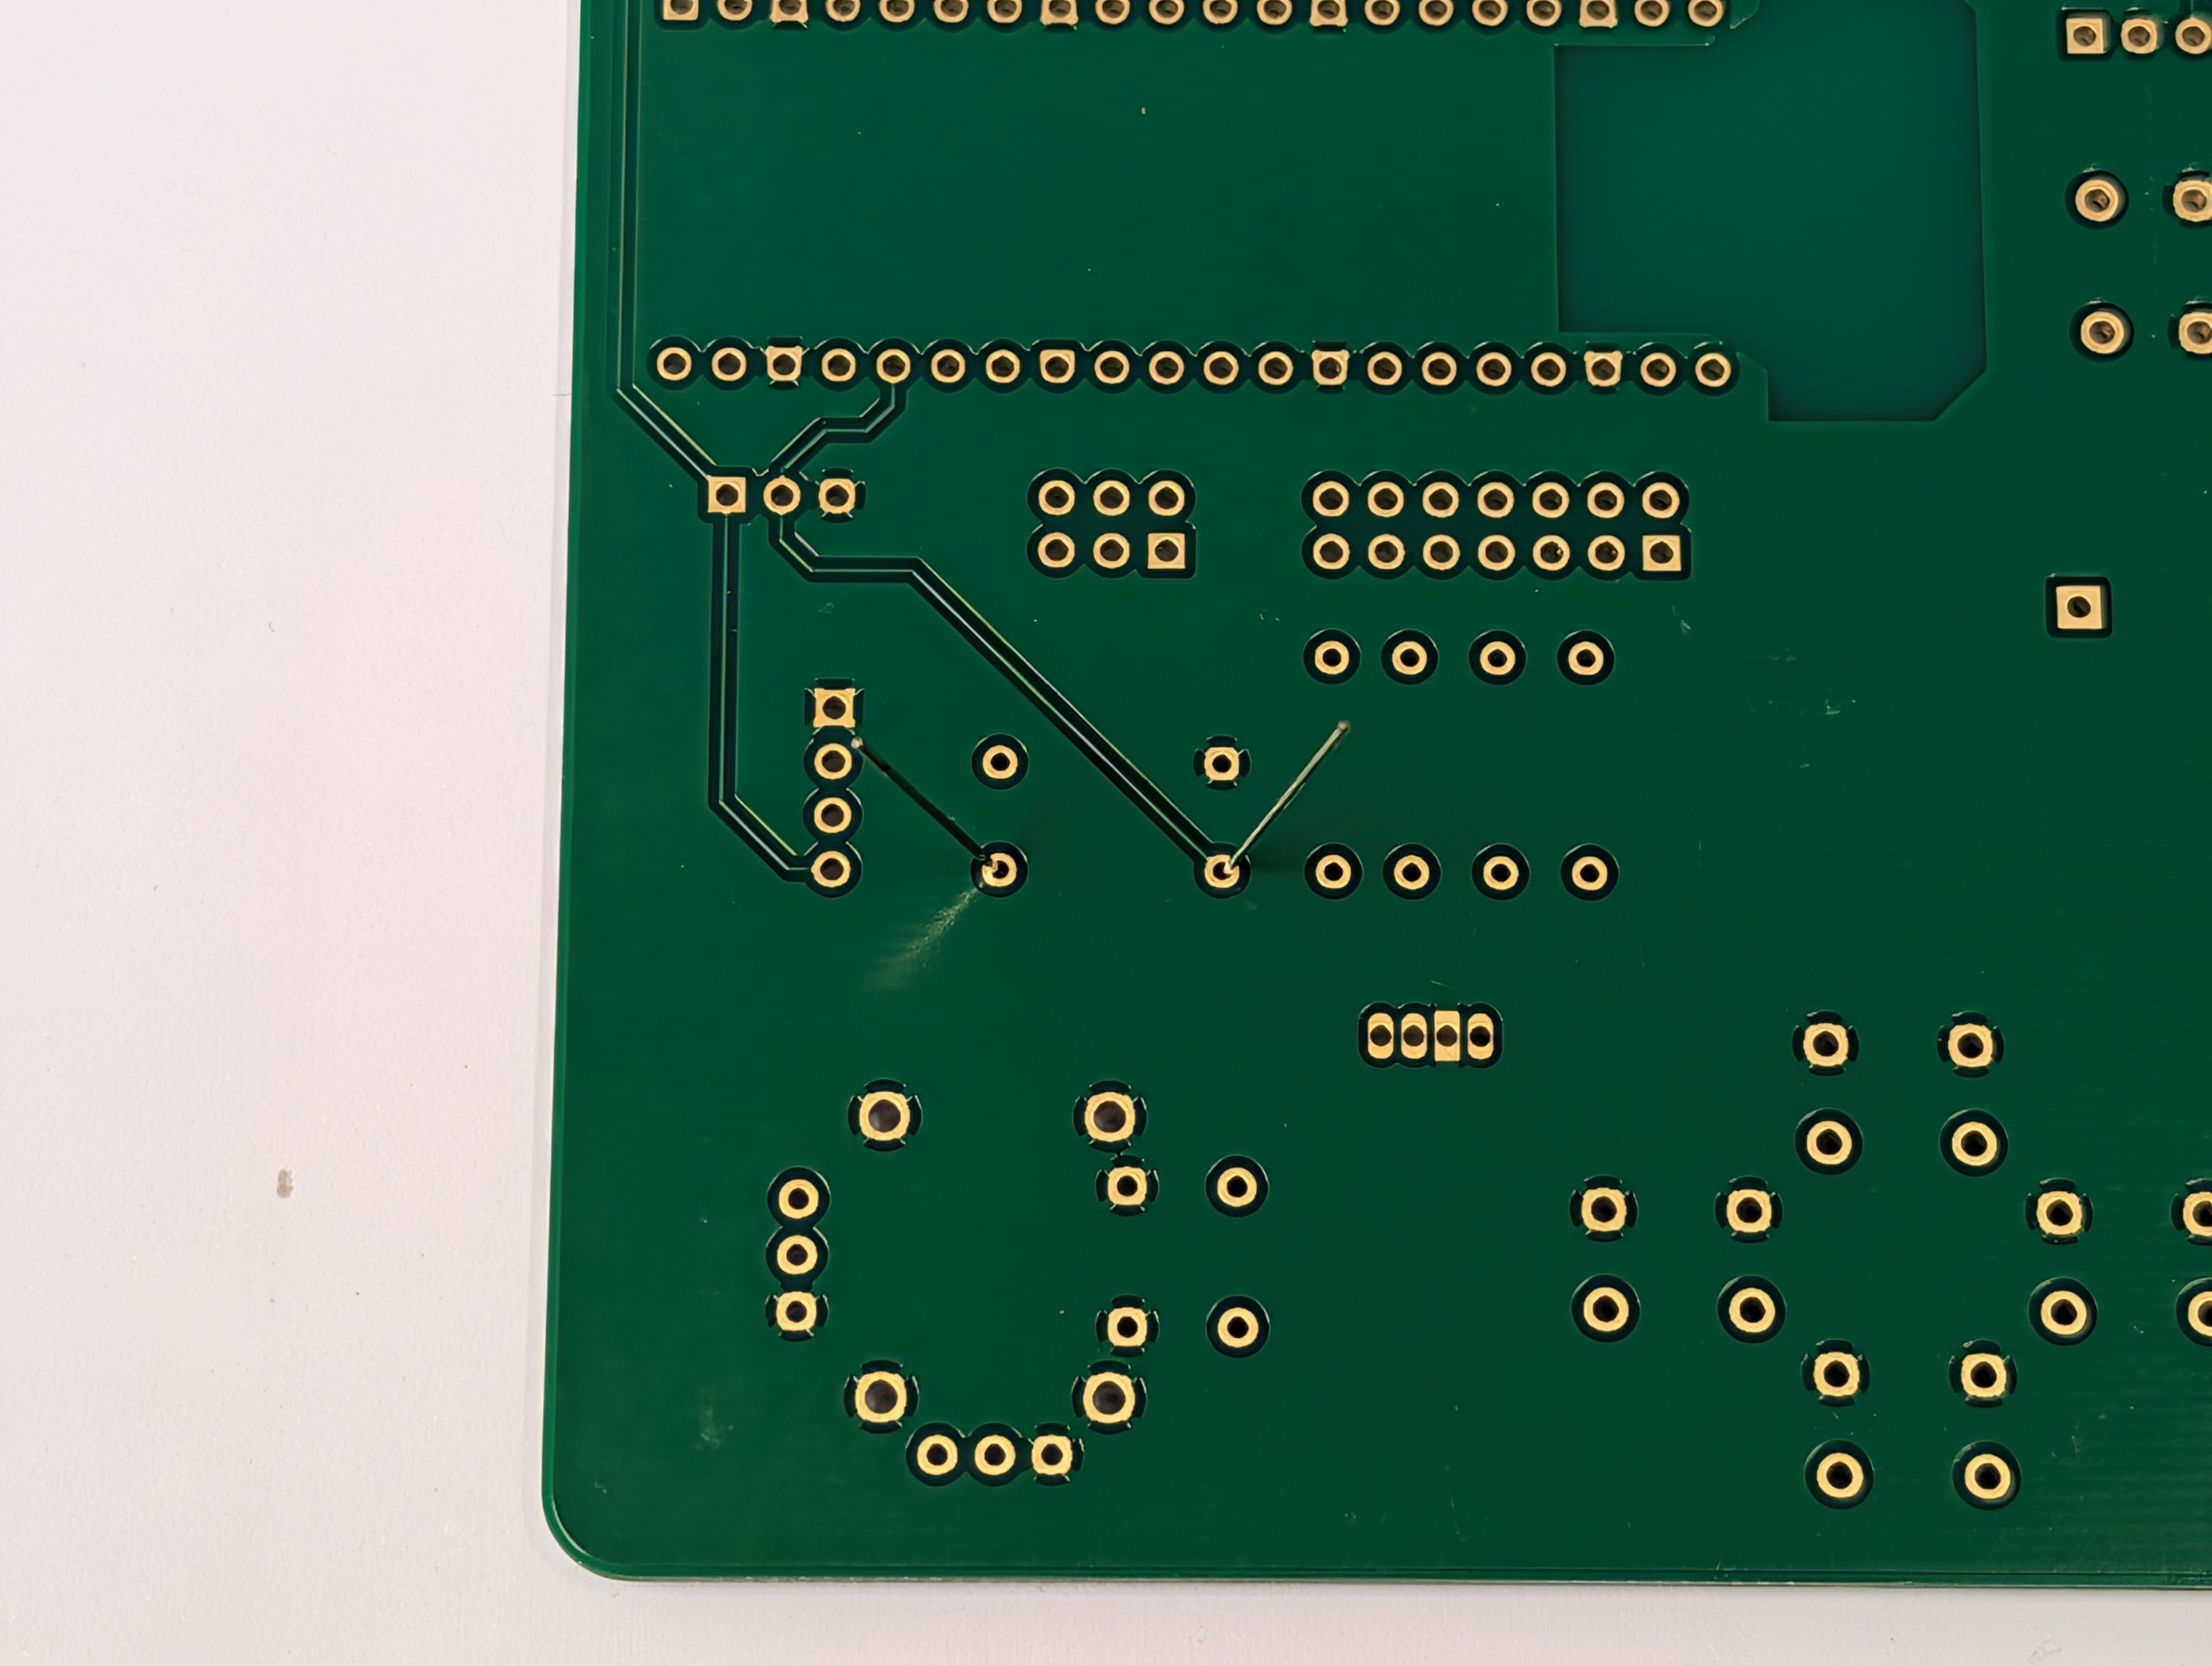
\includegraphics[width=0.75\textwidth]{pictures_of_construction/instruction_step_23.jpg}
\end{figure}

\begin{figure}[H]
    \centering
    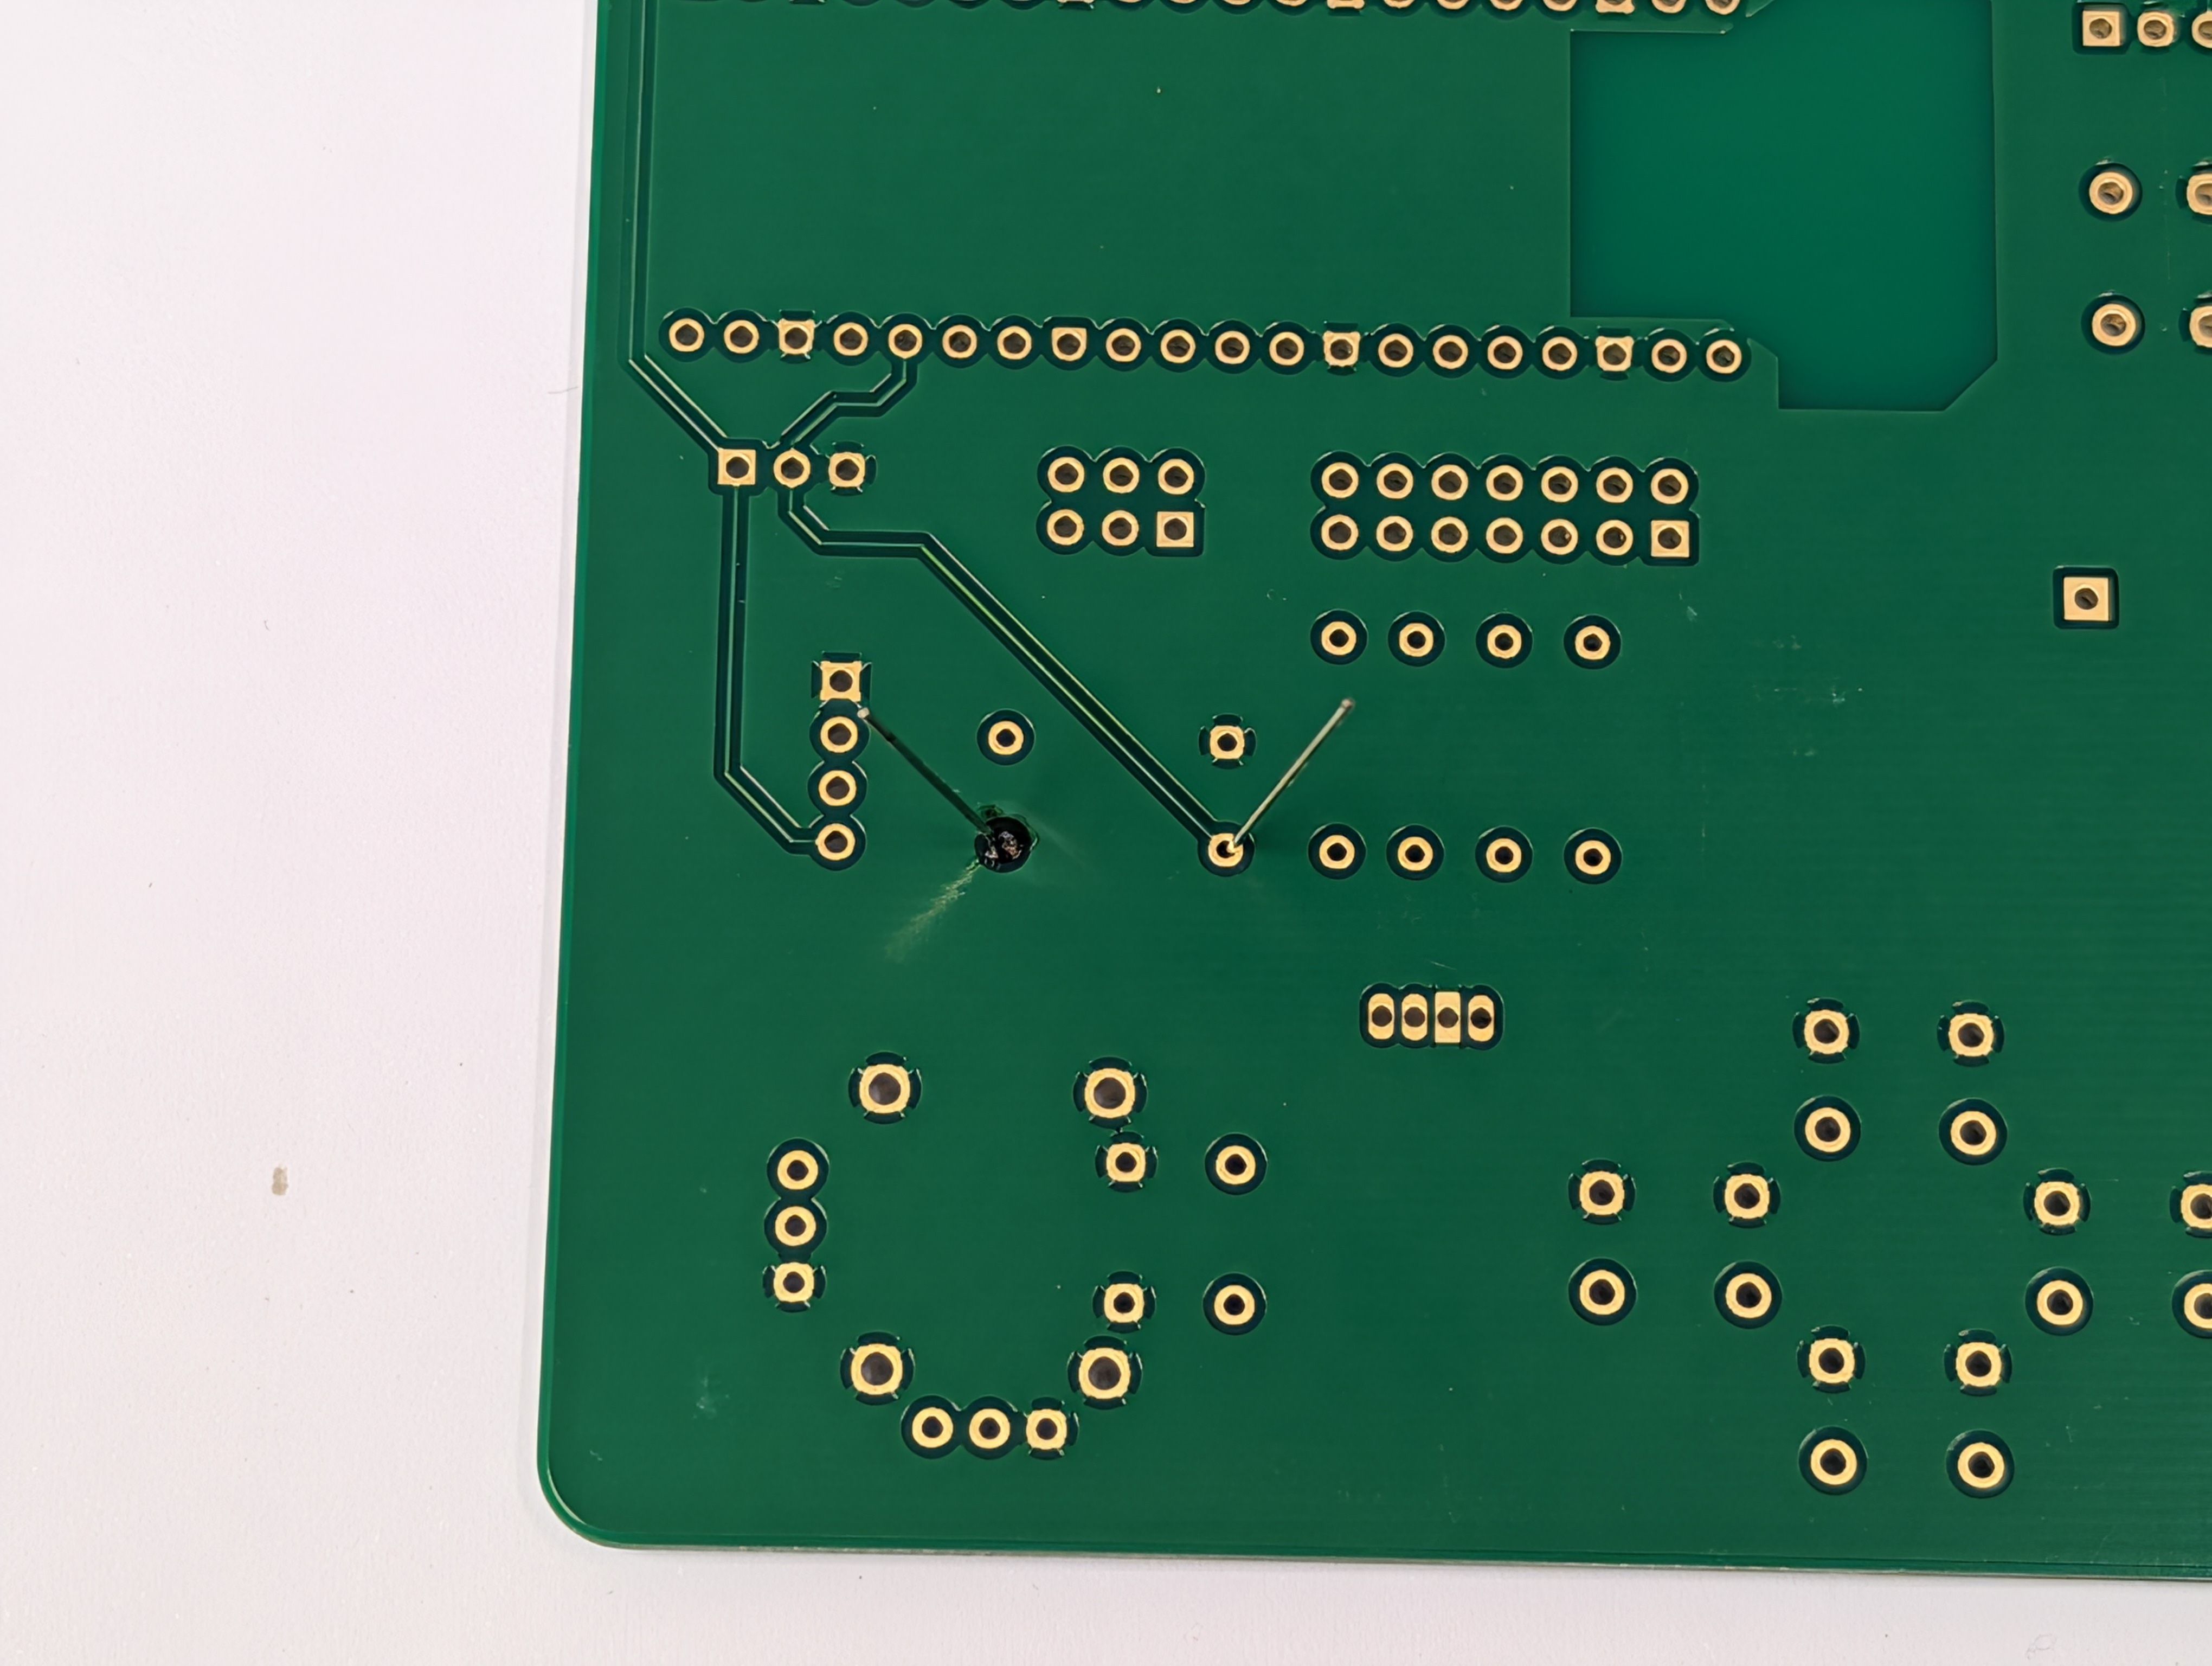
\includegraphics[width=0.75\textwidth]{pictures_of_construction/instruction_step_24.jpg}
\end{figure}

\begin{figure}[H]
    \centering
    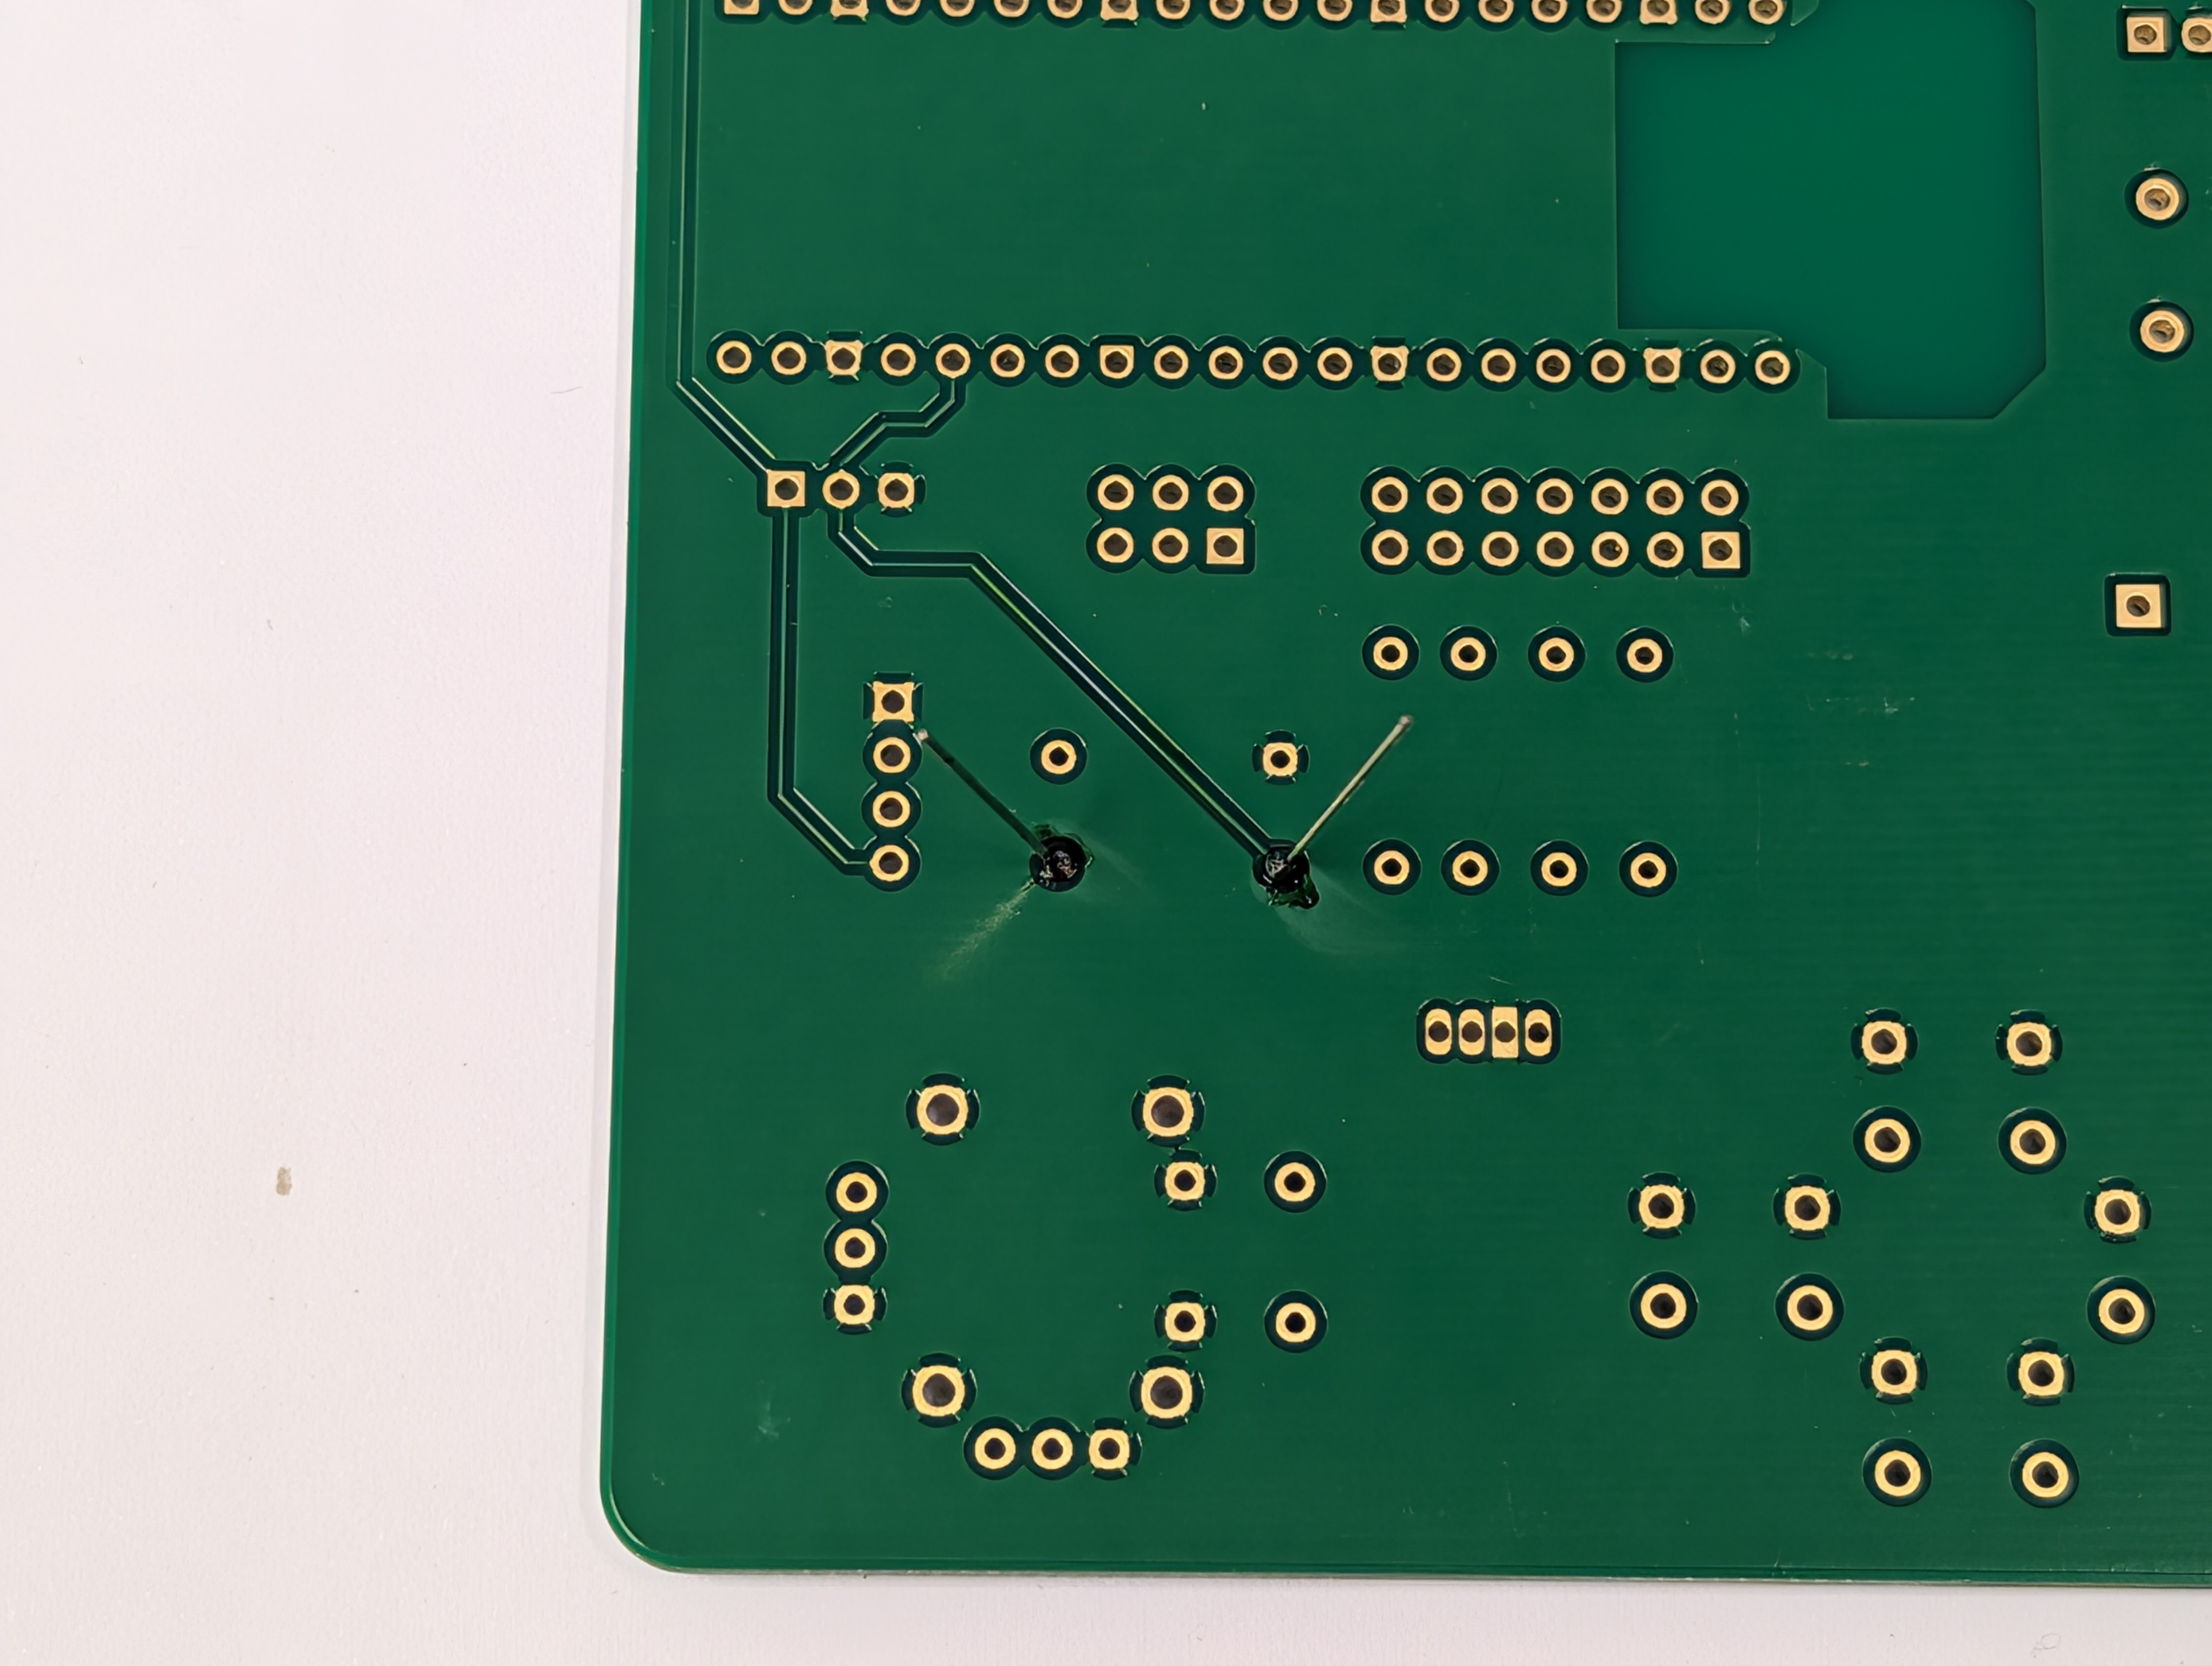
\includegraphics[width=0.75\textwidth]{pictures_of_construction/instruction_step_25.jpg}
\end{figure}

\begin{figure}[H]
    \centering
    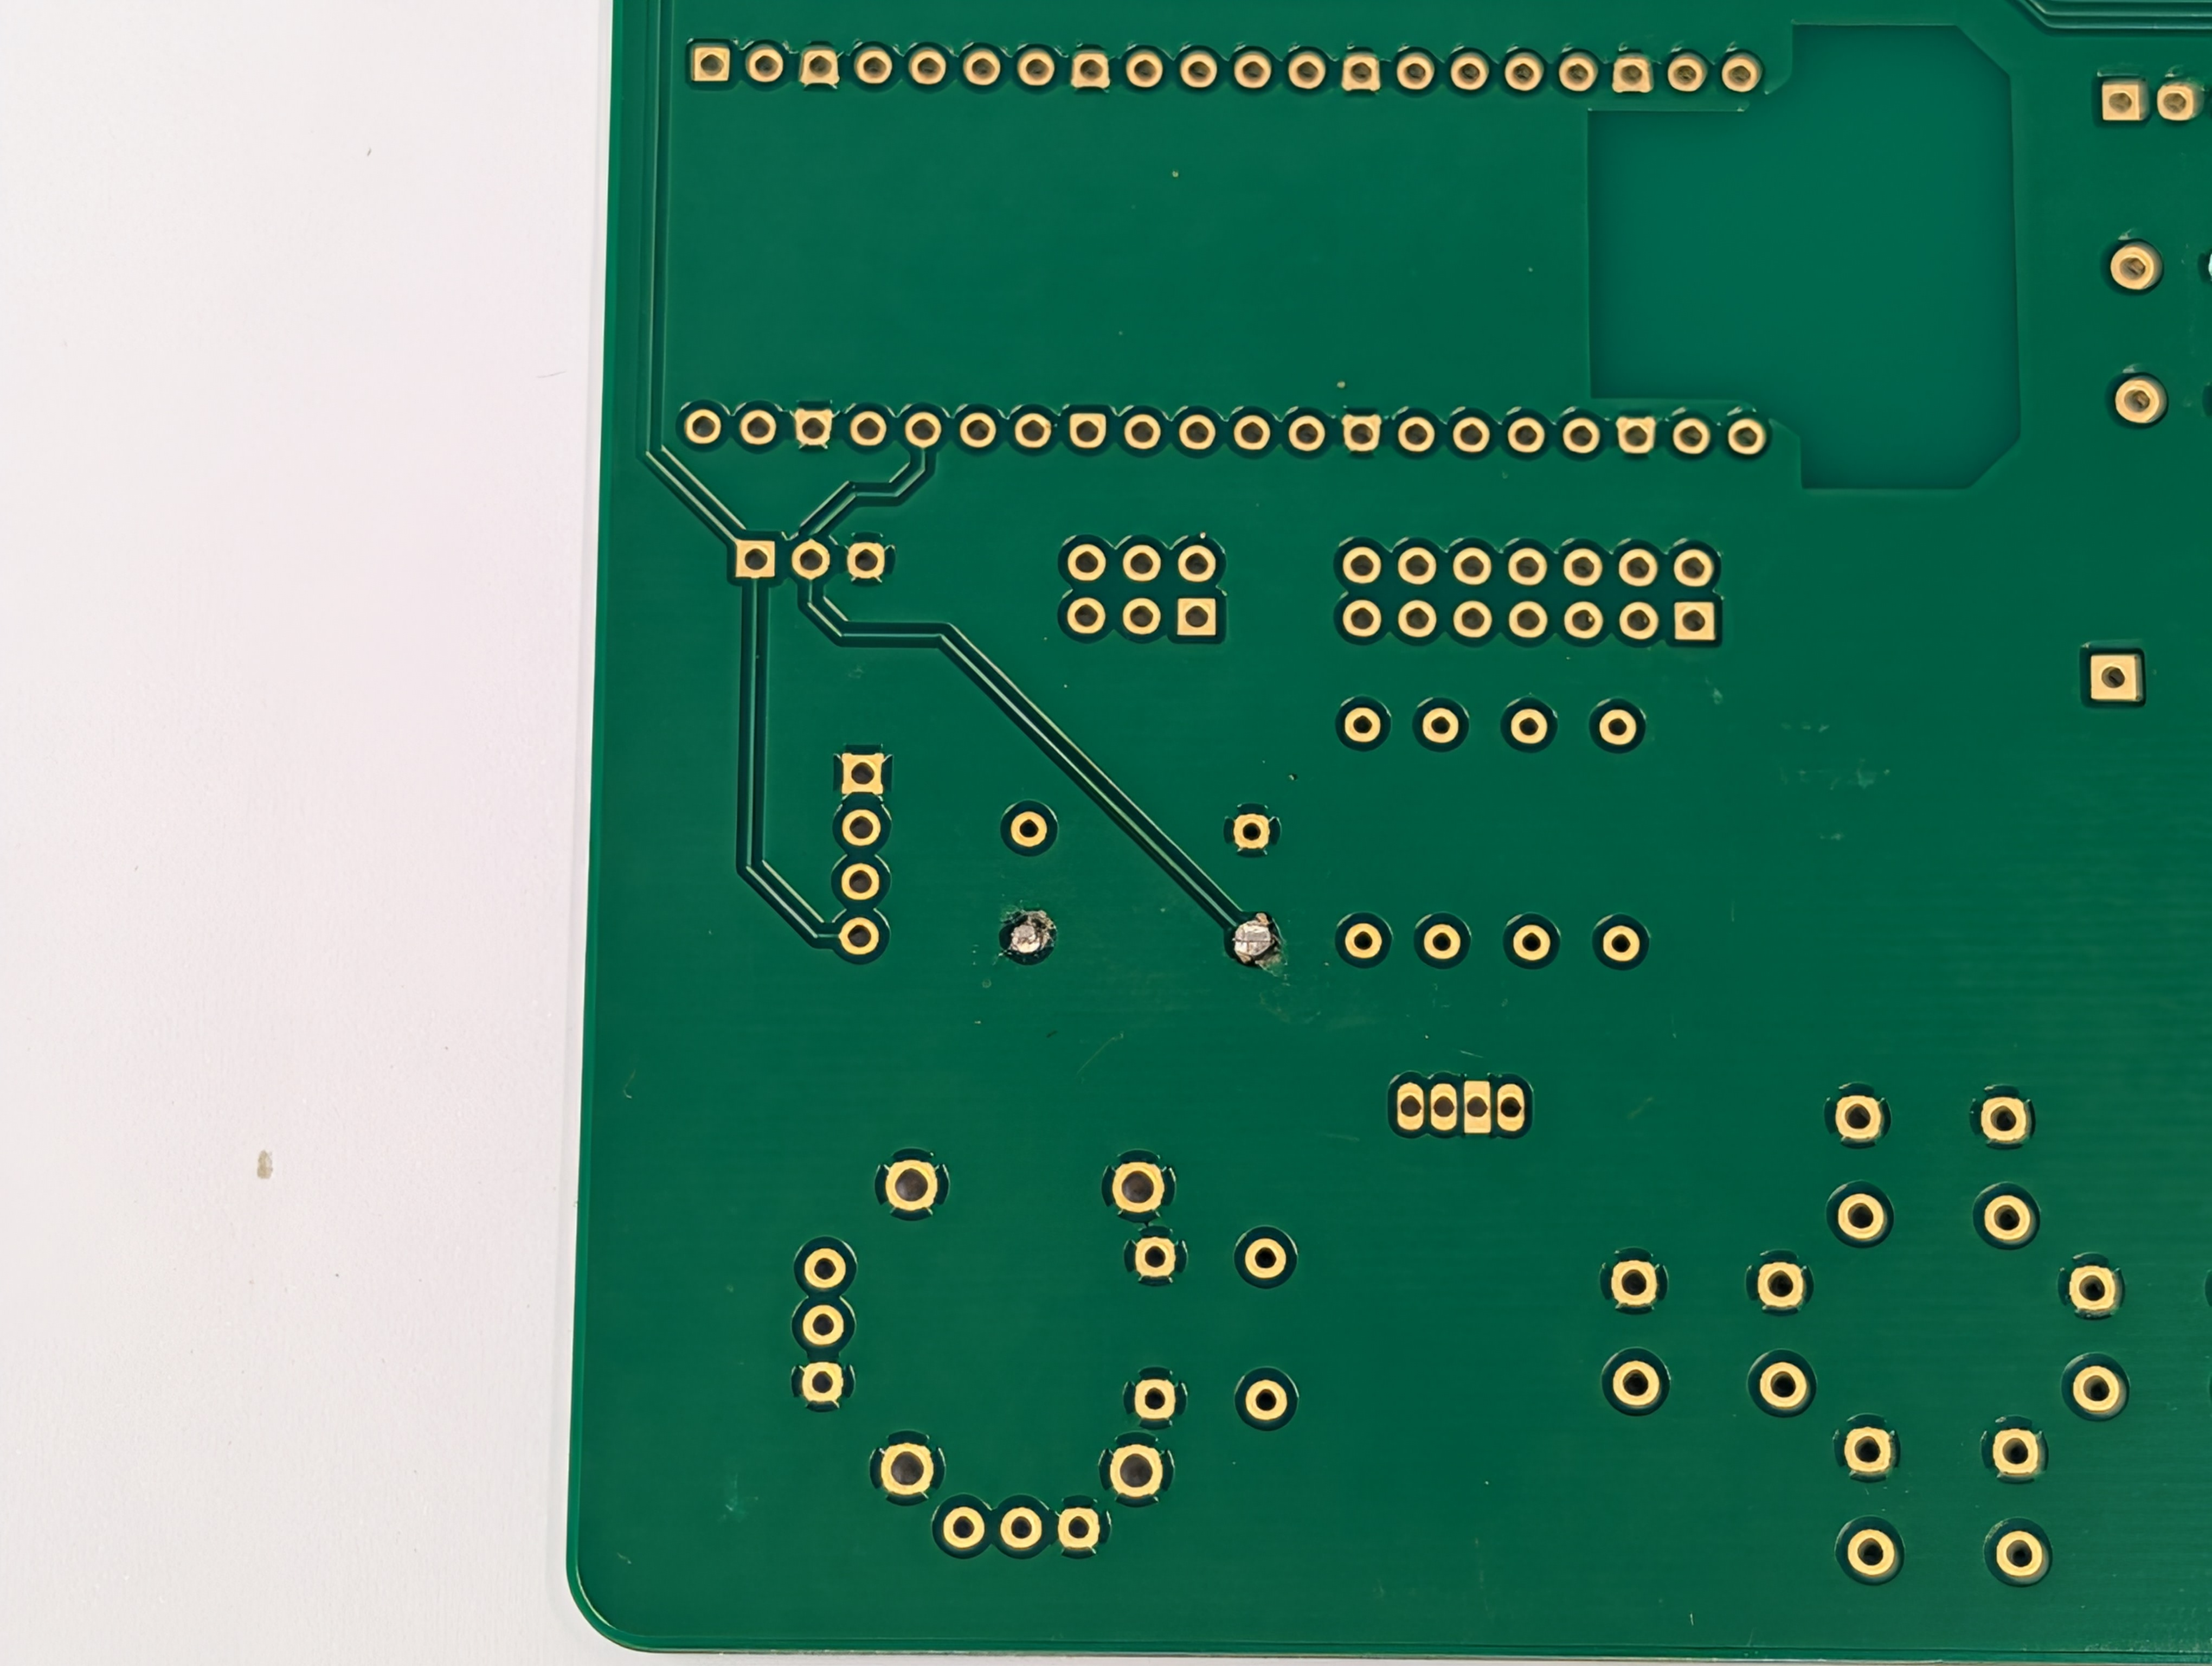
\includegraphics[width=0.75\textwidth]{pictures_of_construction/instruction_step_26.jpg}
\end{figure}

\subsubsection*{5b. 1-k$\Omega$-Widerstand einbauen}

Farbringe:
\begin{itemize}
    \item Braun
    \item Schwarz
    \item Rot
    \item Gold
\end{itemize}

Diesen Widerstand an die passende markierte Stelle setzen und einlöten.

\begin{figure}[H]
    \centering
    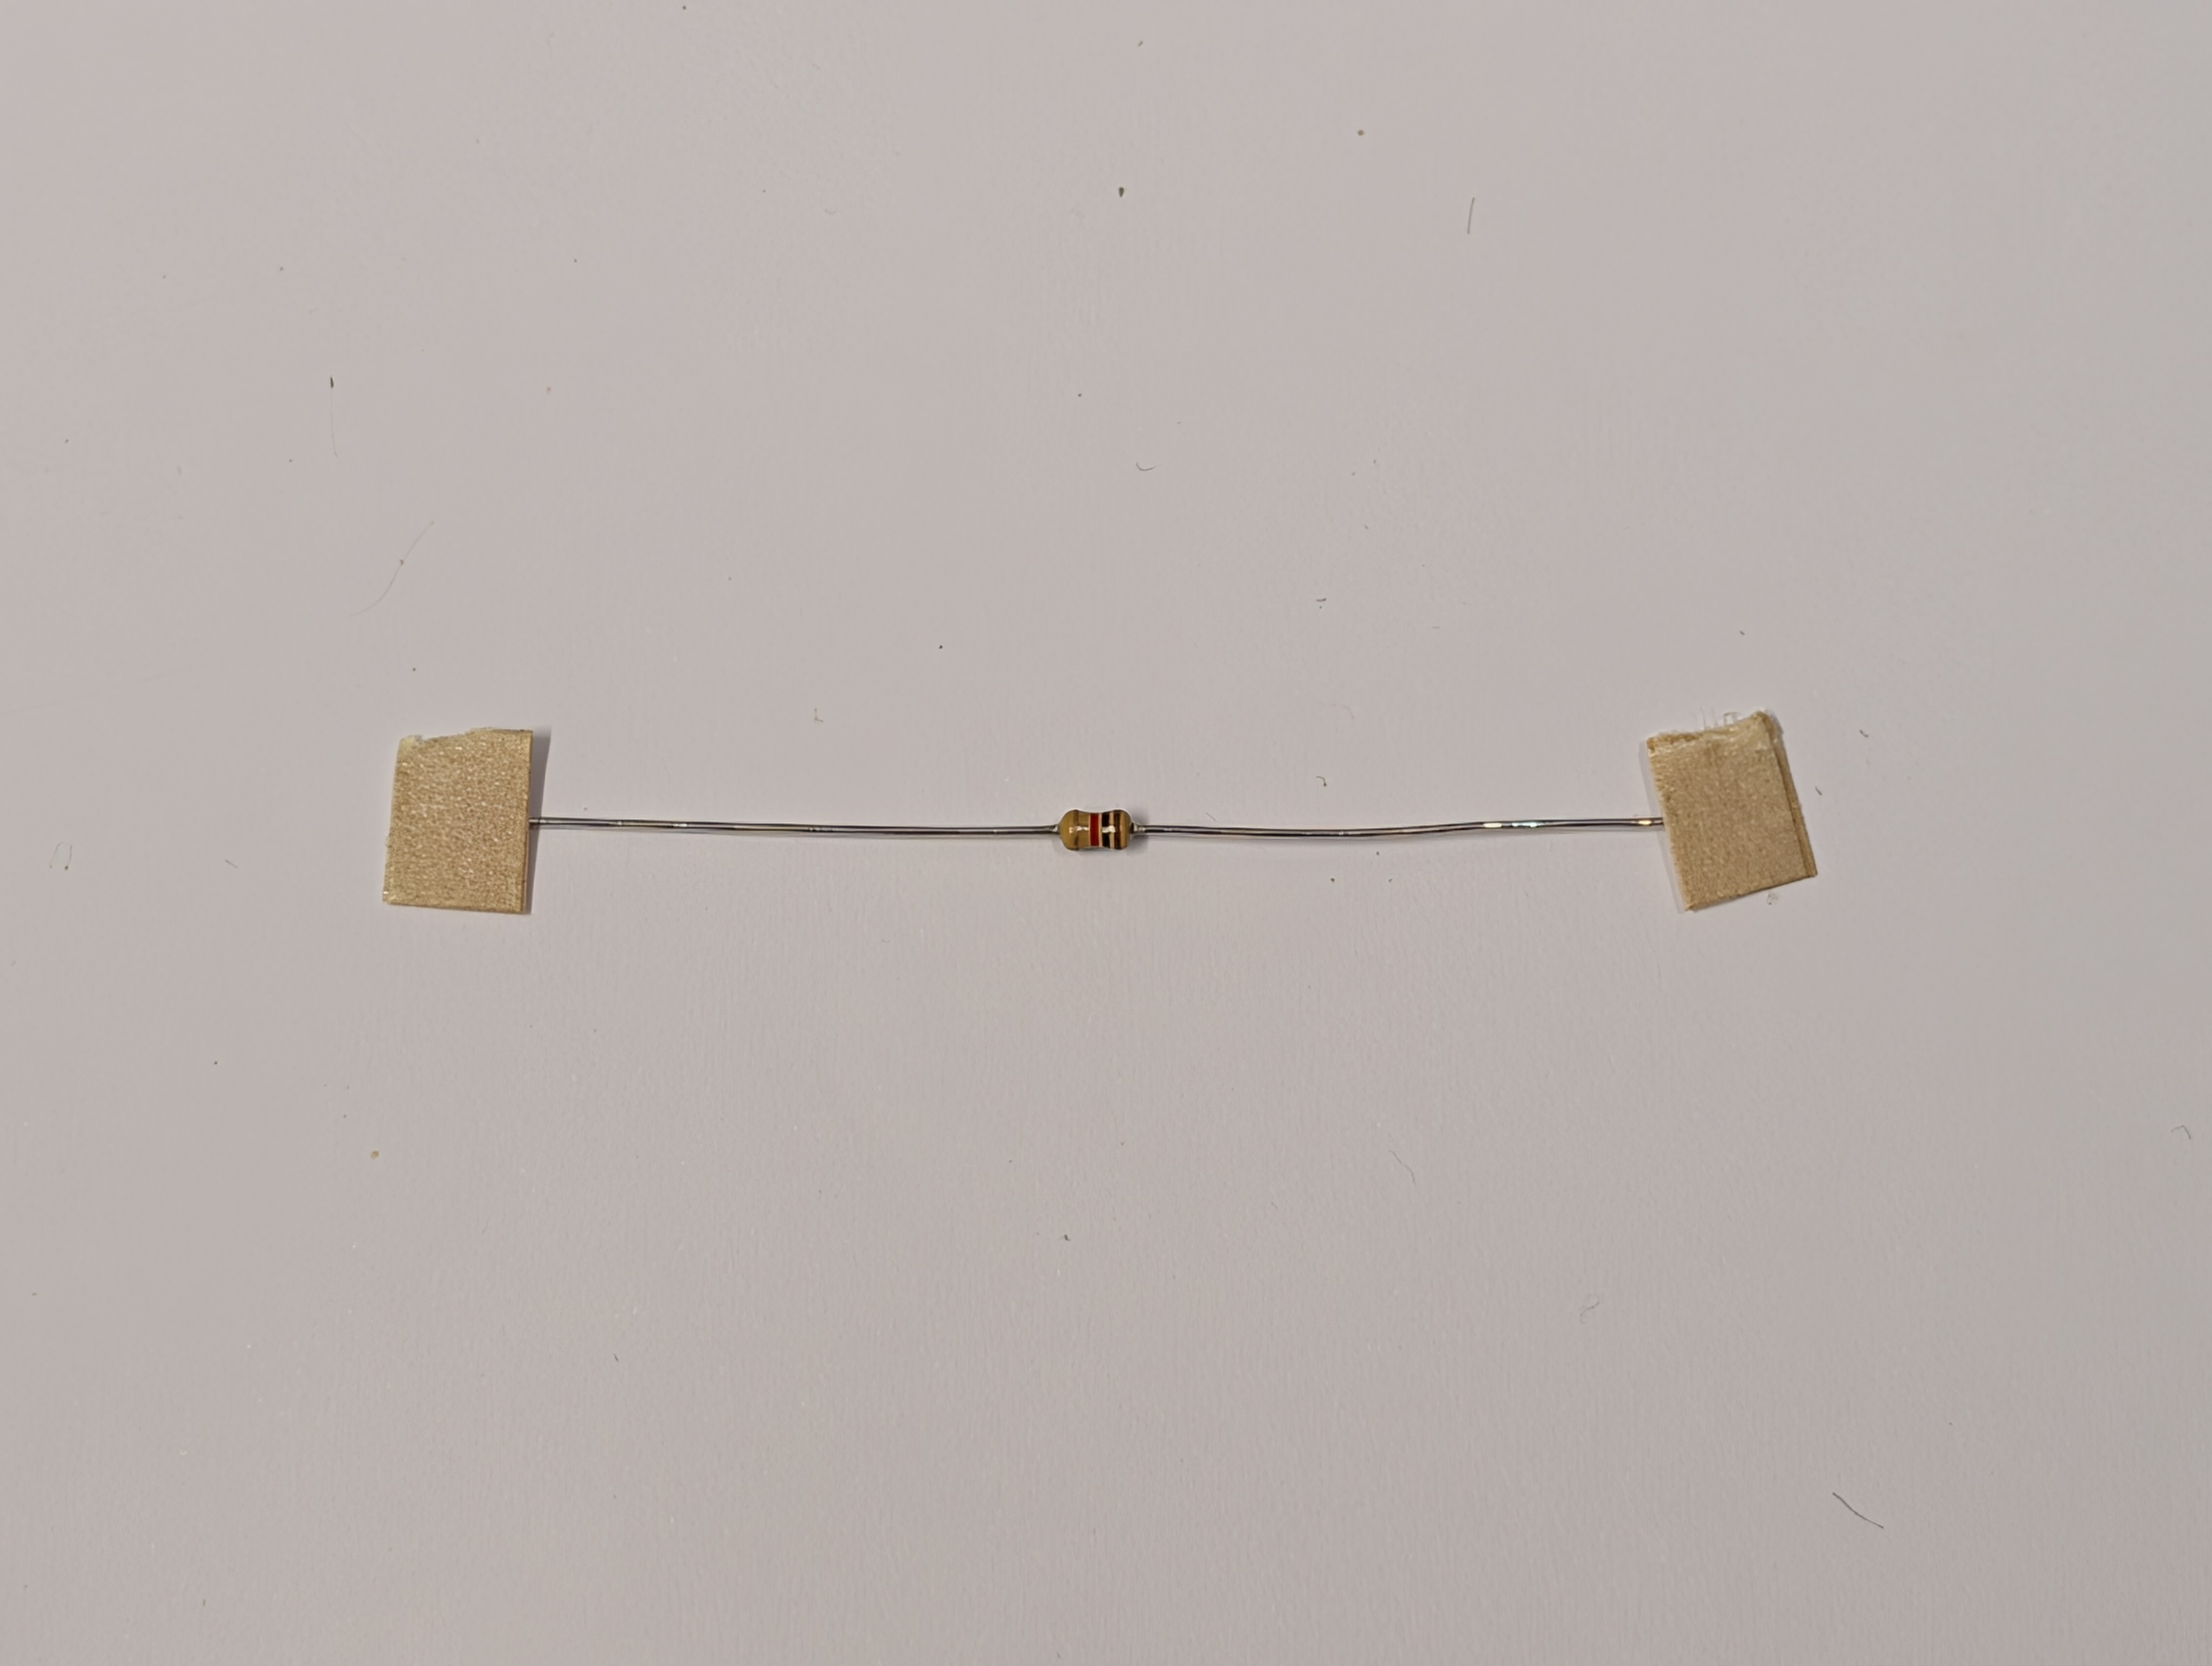
\includegraphics[width=0.75\textwidth]{pictures_of_construction/instruction_step_27.jpg}
\end{figure}

\begin{figure}[H]
    \centering
    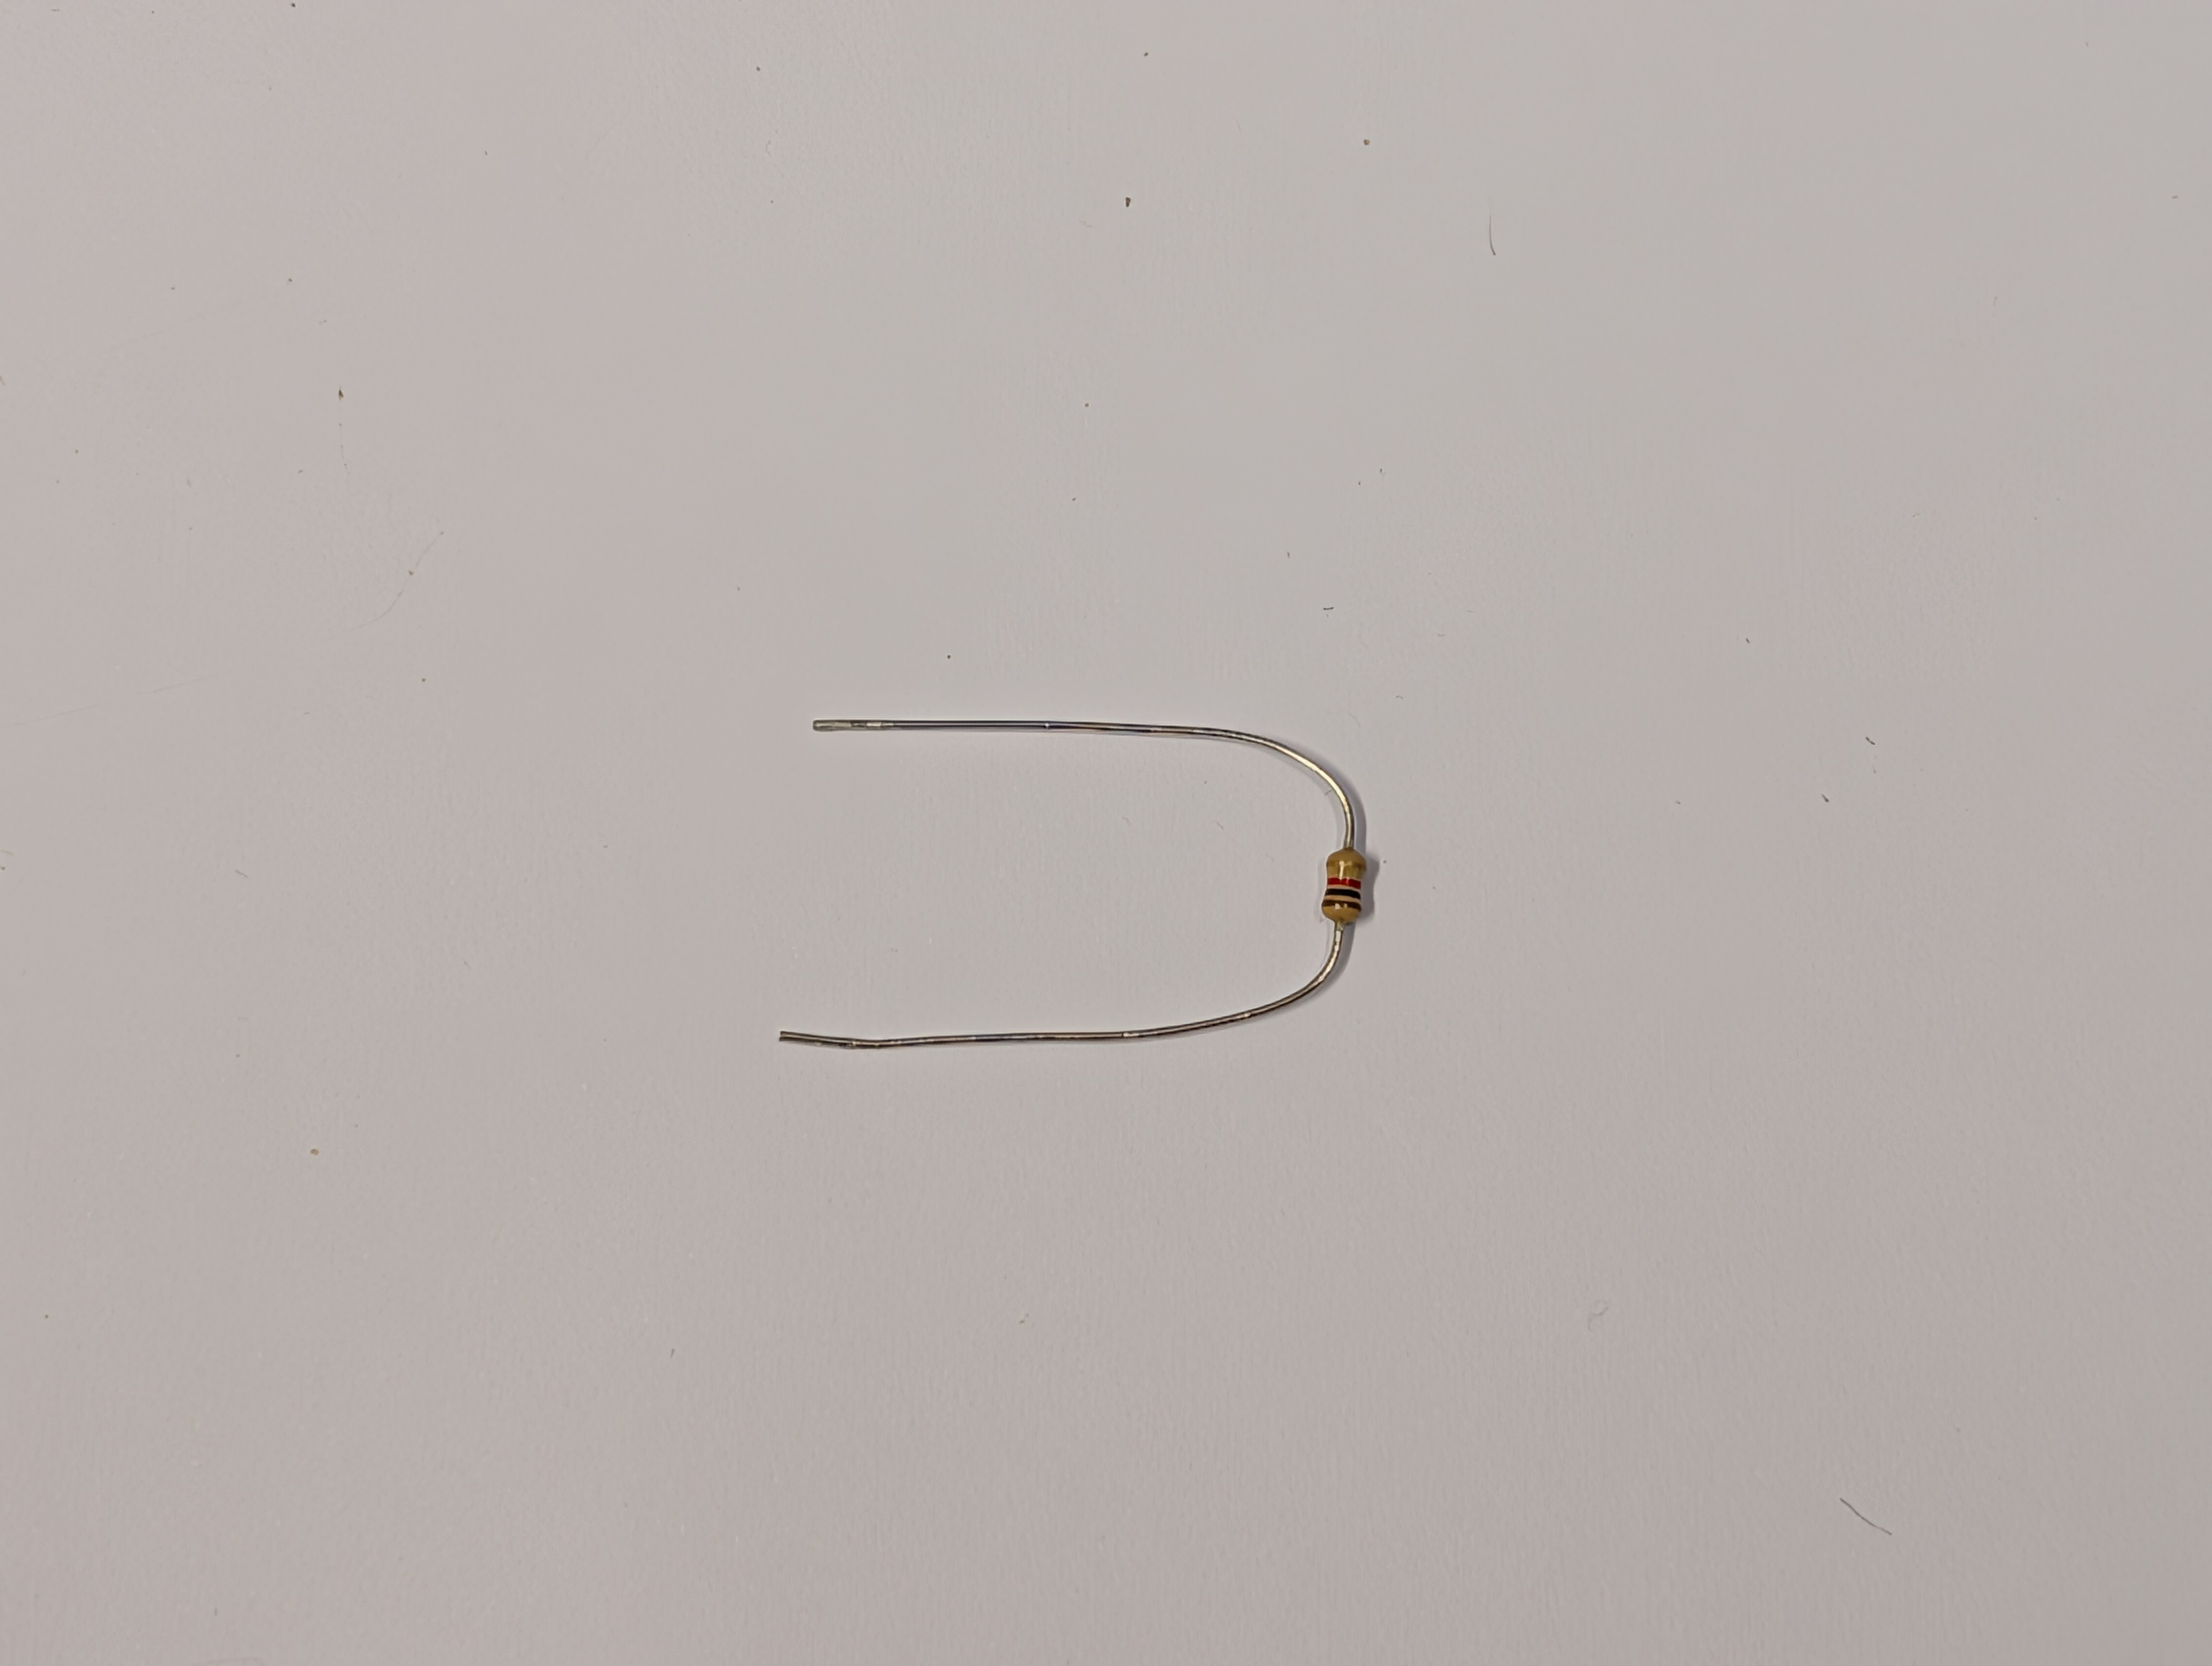
\includegraphics[width=0.75\textwidth]{pictures_of_construction/instruction_step_28.jpg}
\end{figure}

\begin{figure}[H]
    \centering
    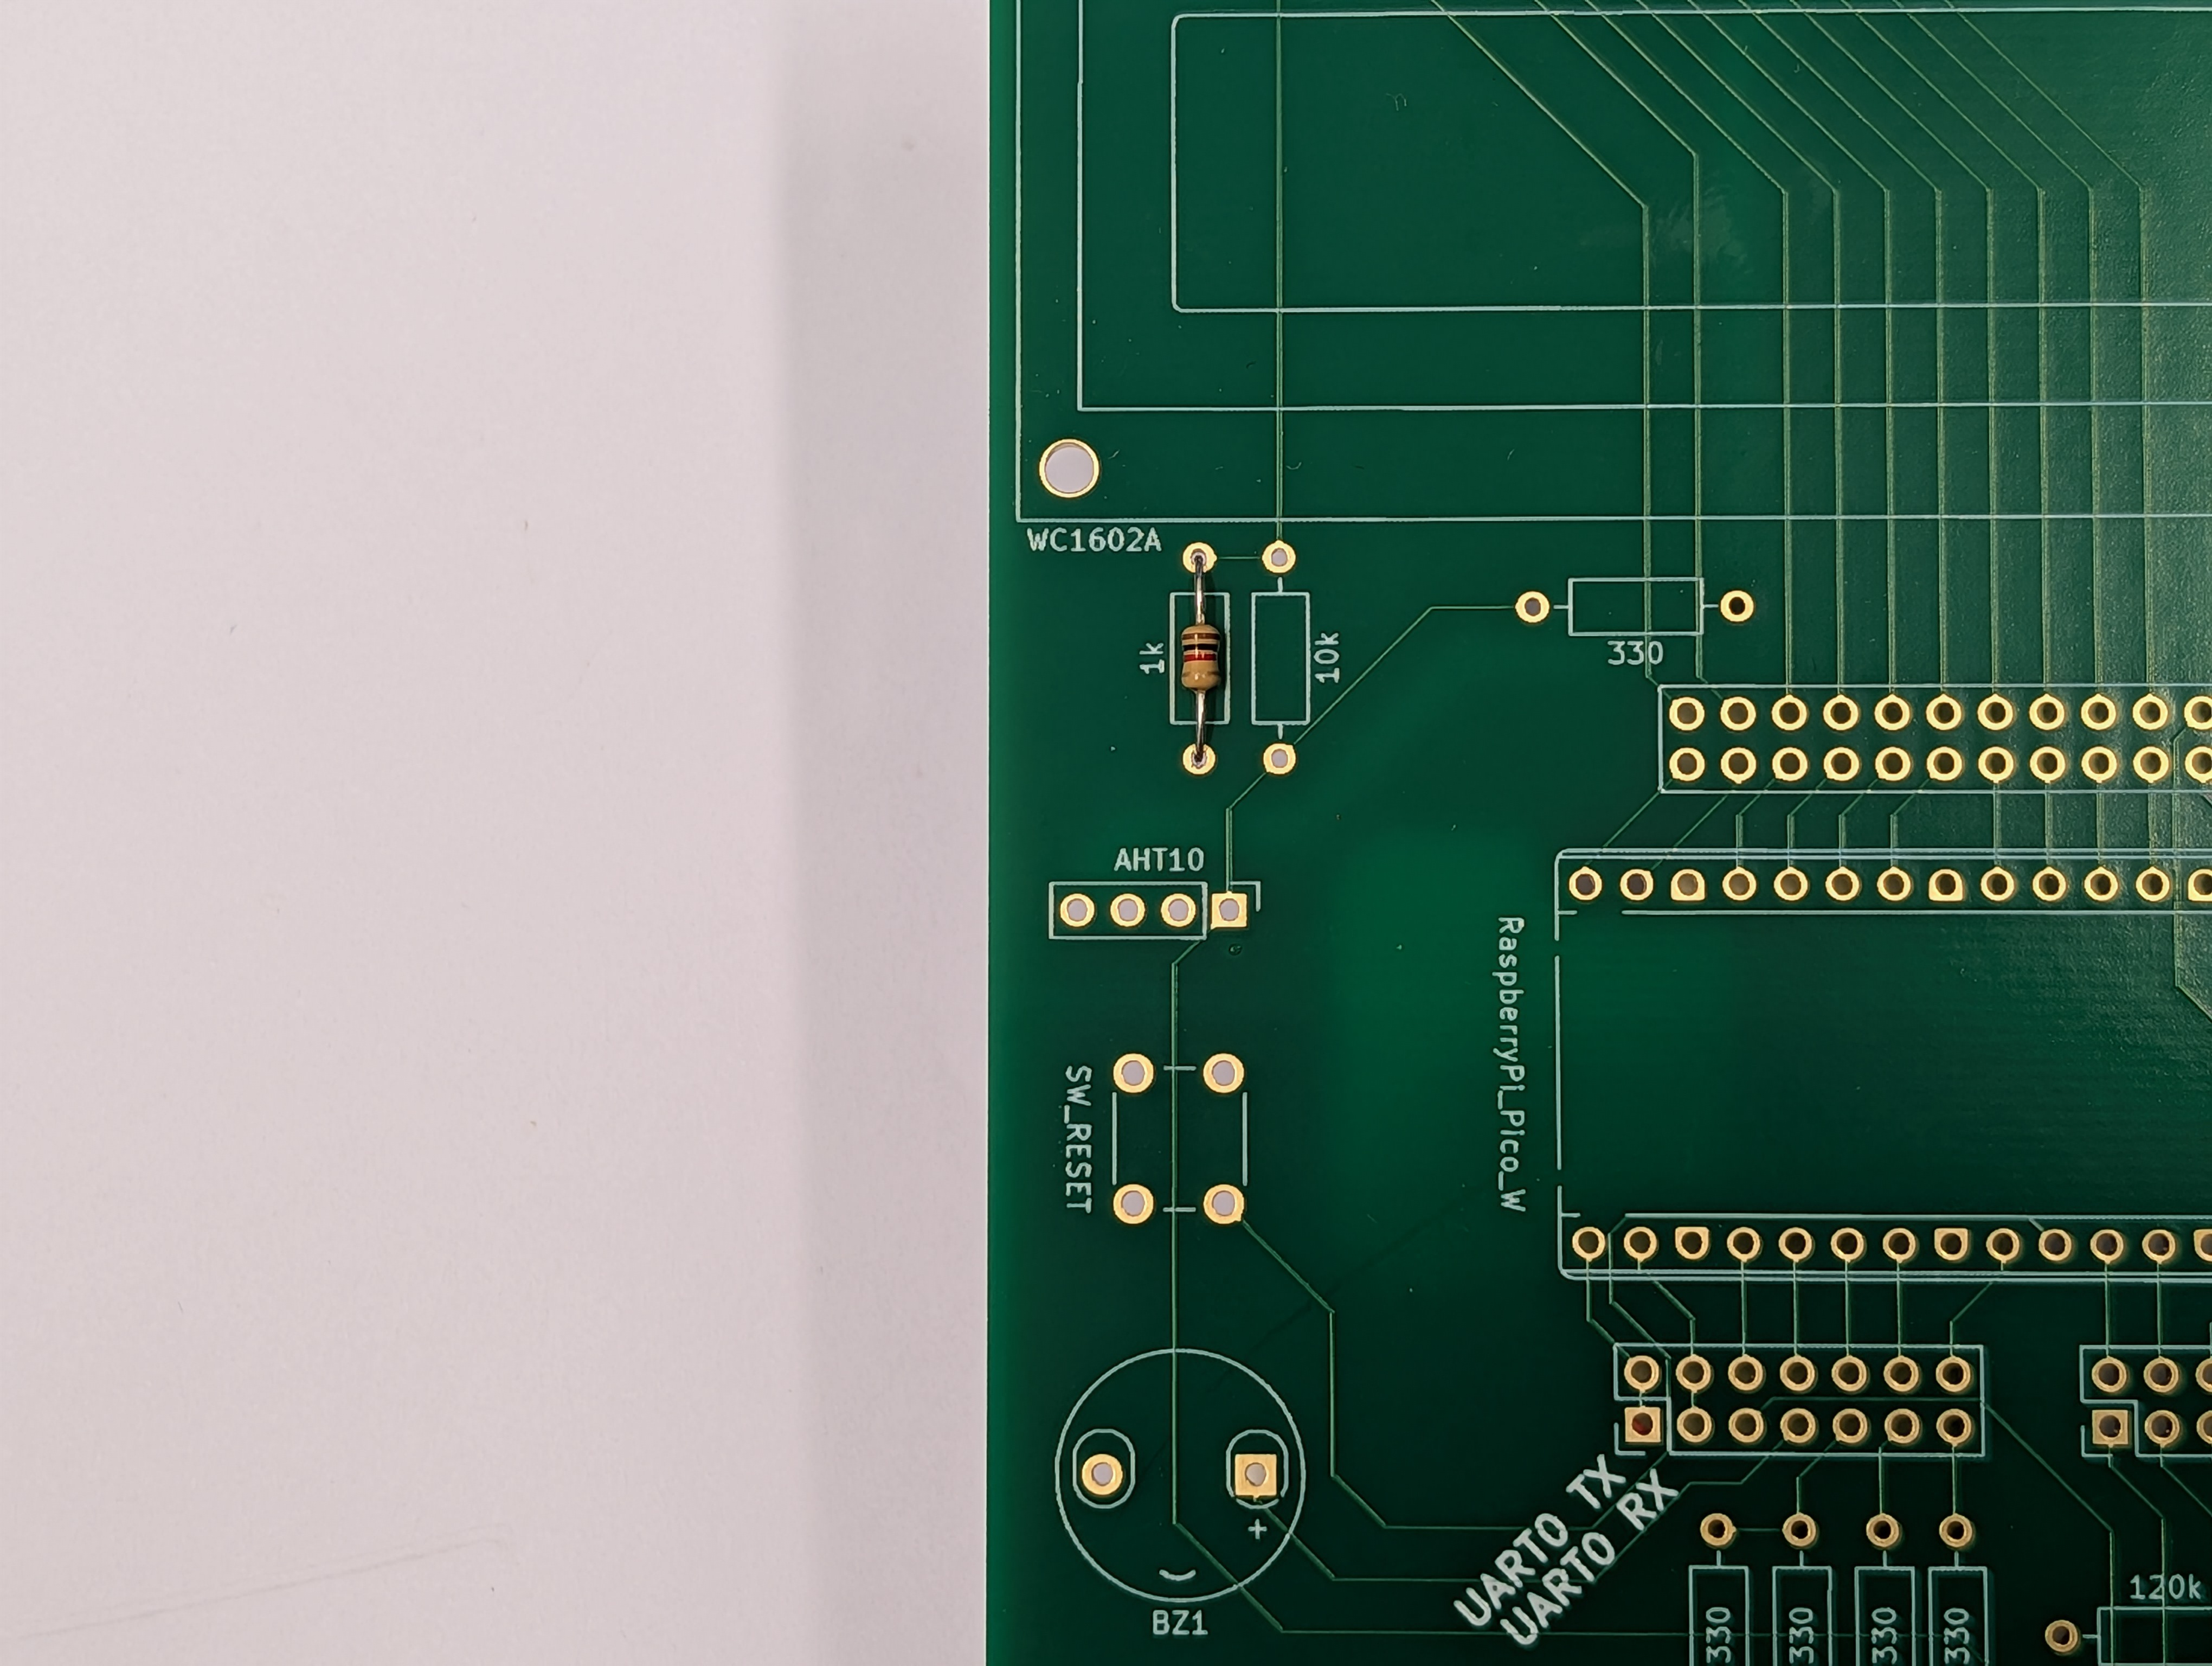
\includegraphics[width=0.75\textwidth]{pictures_of_construction/instruction_step_29.jpg}
\end{figure}

\subsubsection*{5c. 10-k$\Omega$-Widerstand einbauen}

Farbringe:
\begin{itemize}
    \item Braun
    \item Schwarz
    \item Orange
    \item Gold
\end{itemize}

Auch hier:
\begin{itemize}
    \item biegen
    \item einsetzen
    \item löten
    \item Drähte abschneiden
\end{itemize}

\begin{figure}[H]
    \centering
    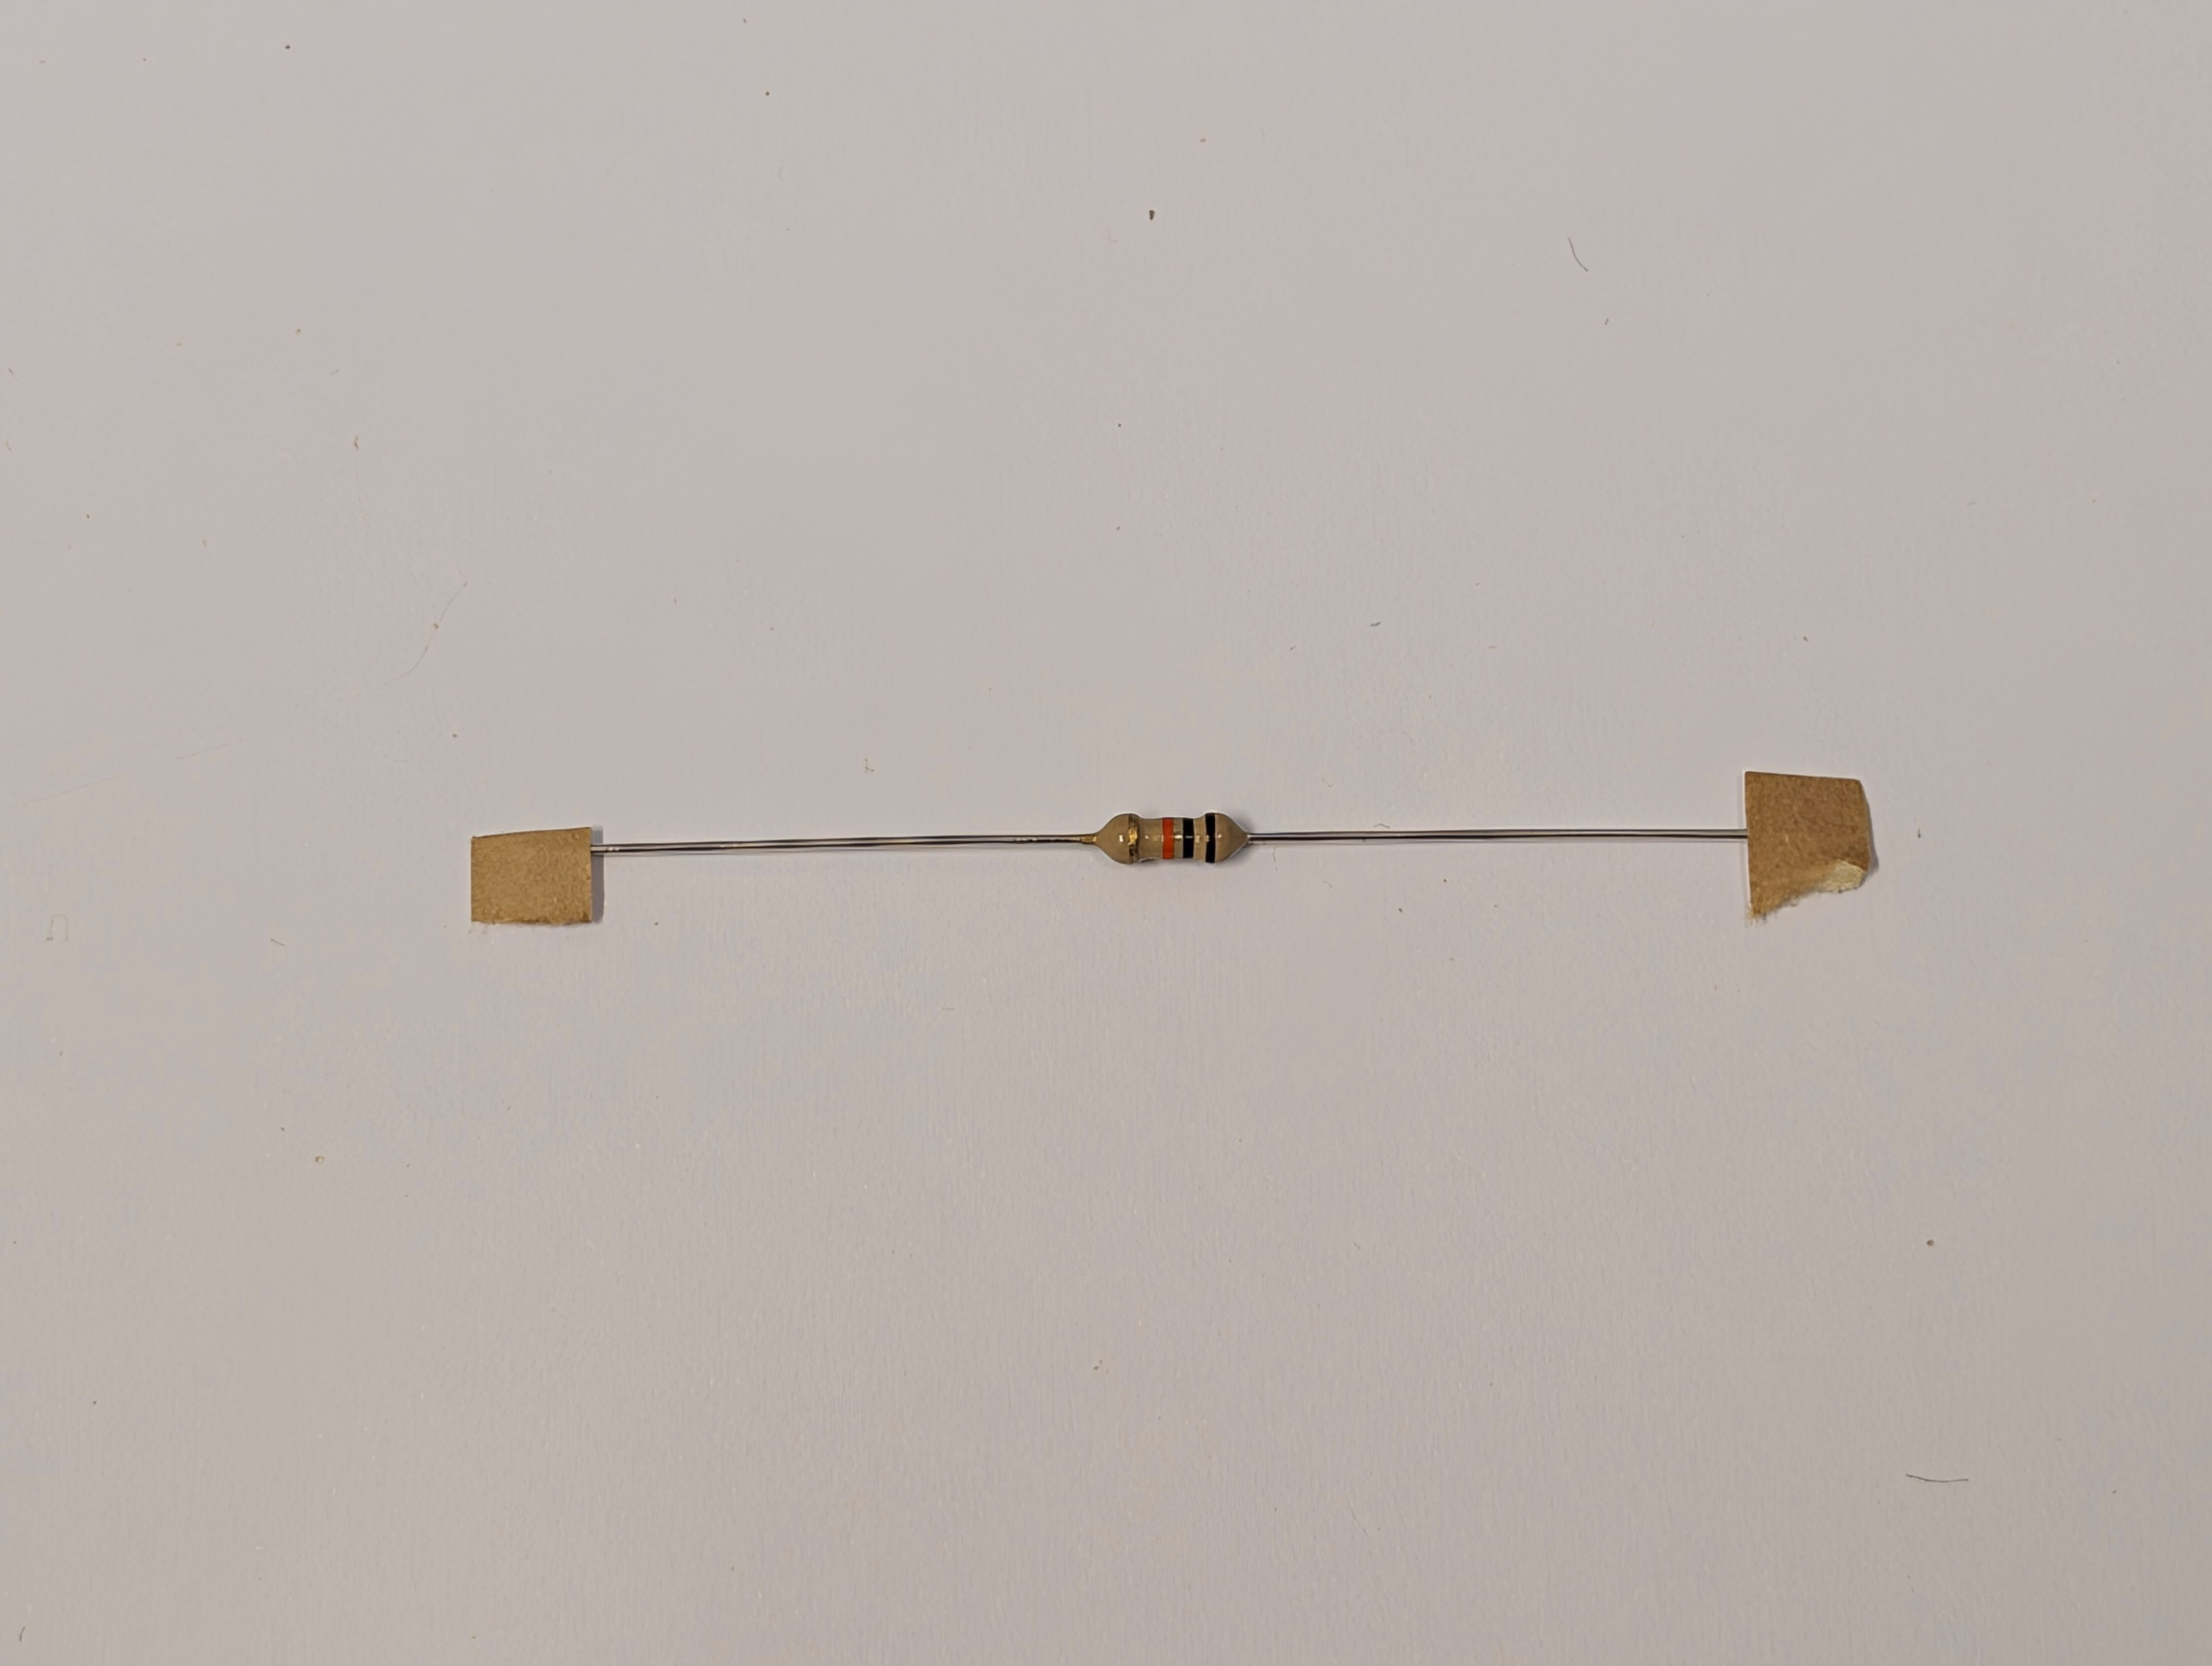
\includegraphics[width=0.75\textwidth]{pictures_of_construction/instruction_step_30.jpg}
\end{figure}

\begin{figure}[H]
    \centering
    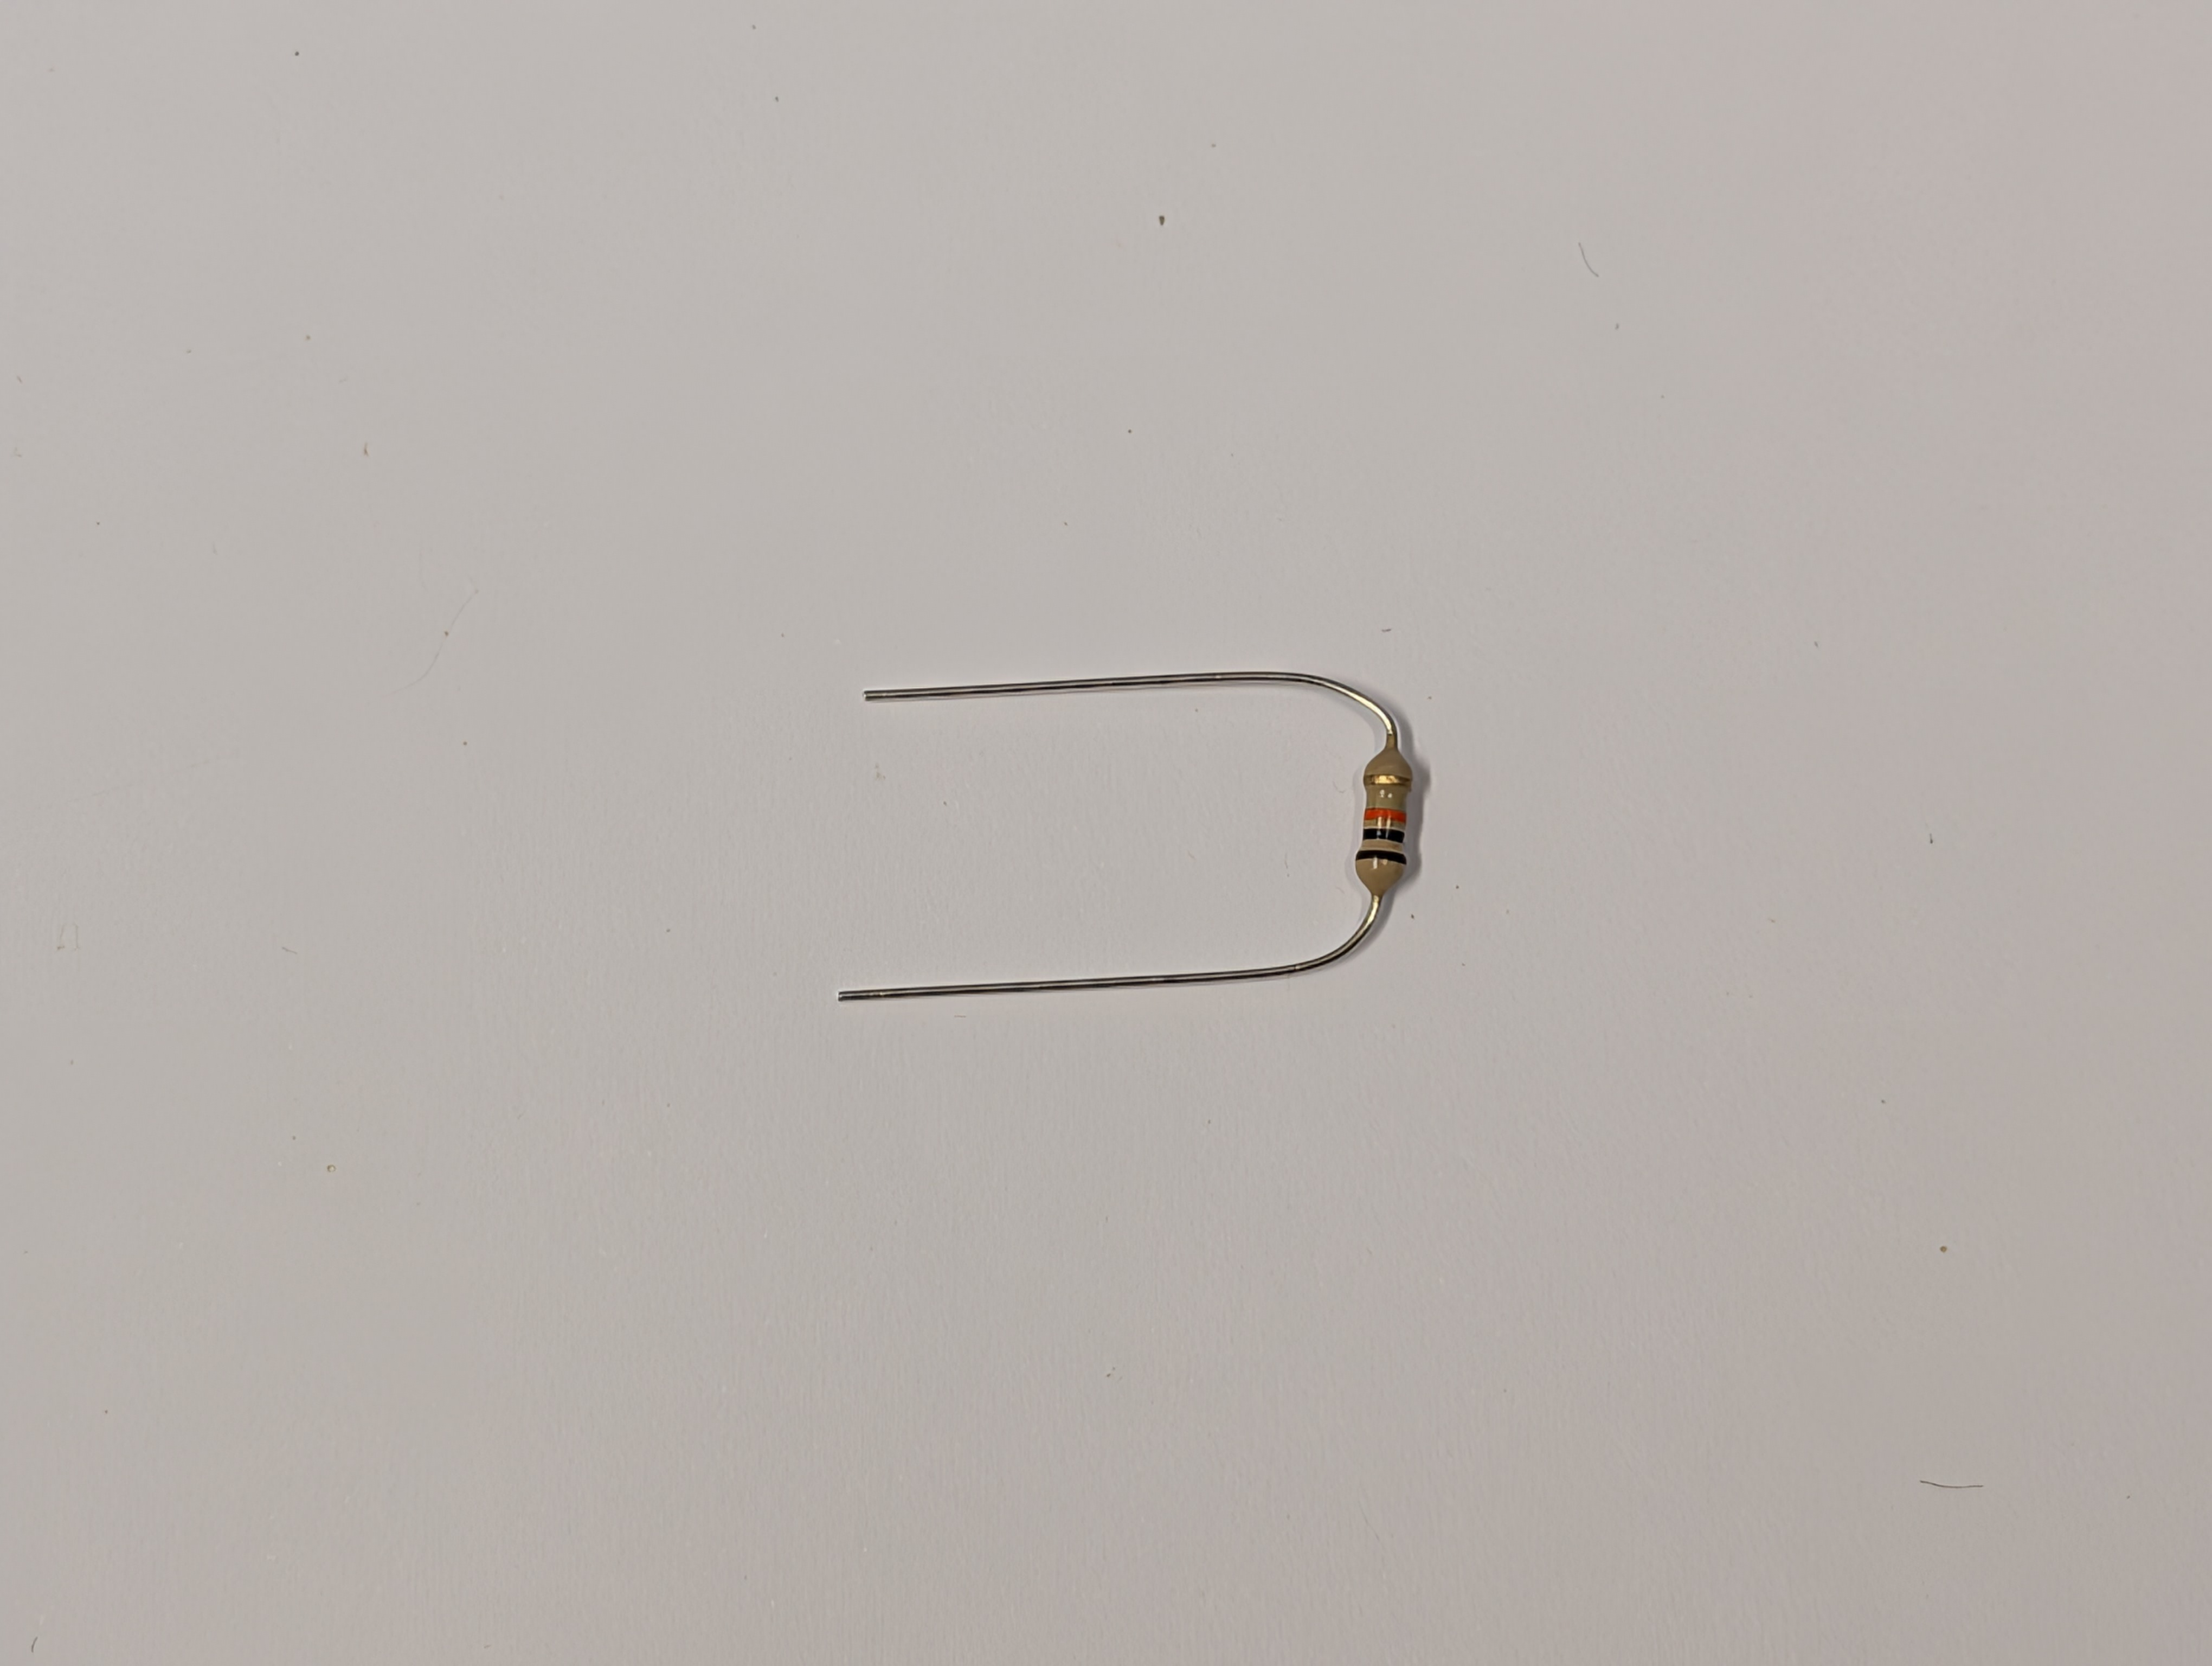
\includegraphics[width=0.75\textwidth]{pictures_of_construction/instruction_step_31.jpg}
\end{figure}

\begin{figure}[H]
    \centering
    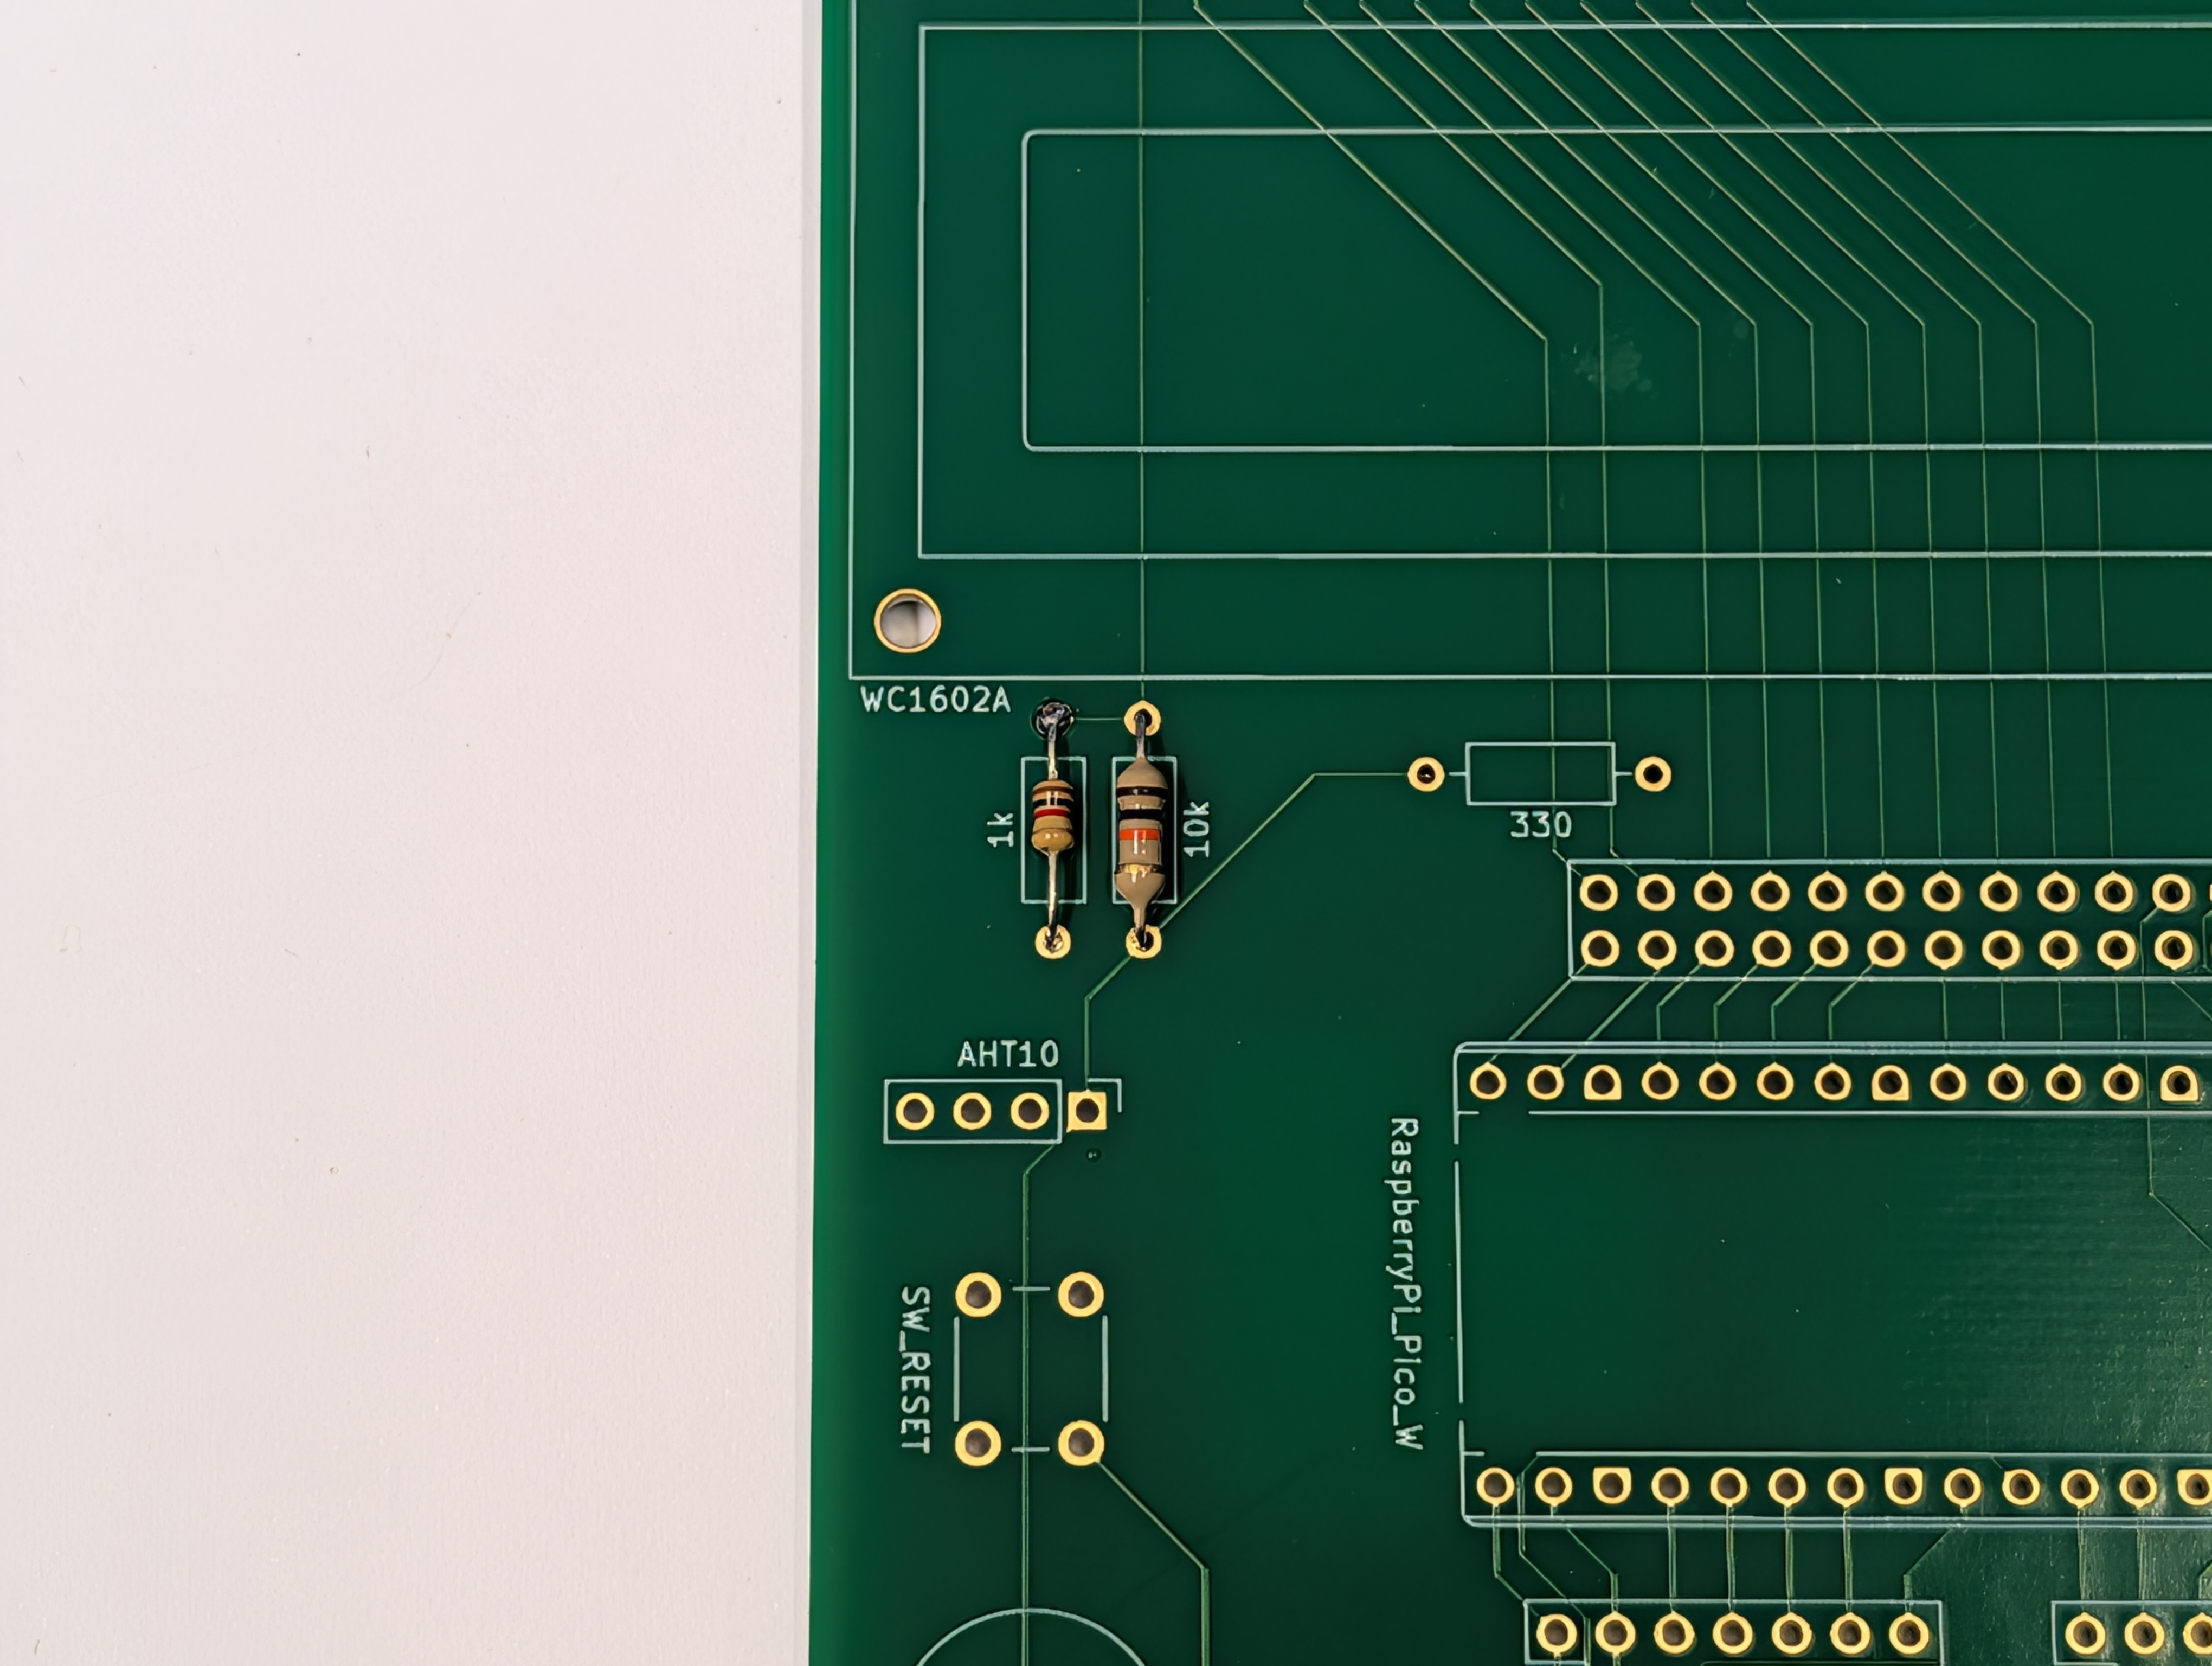
\includegraphics[width=0.75\textwidth]{pictures_of_construction/instruction_step_32.jpg}
\end{figure}

\subsubsection*{5d. 330-$\Omega$-Widerstände einbauen}

Farbringe:
\begin{itemize}
    \item Orange
    \item Orange
    \item Schwarz
    \item Schwarz
    \item Braun
\end{itemize}

Davon gibt es \textbf{fünf Stück}.\\
Baue alle nacheinander ein.

\begin{figure}[H]
    \centering
    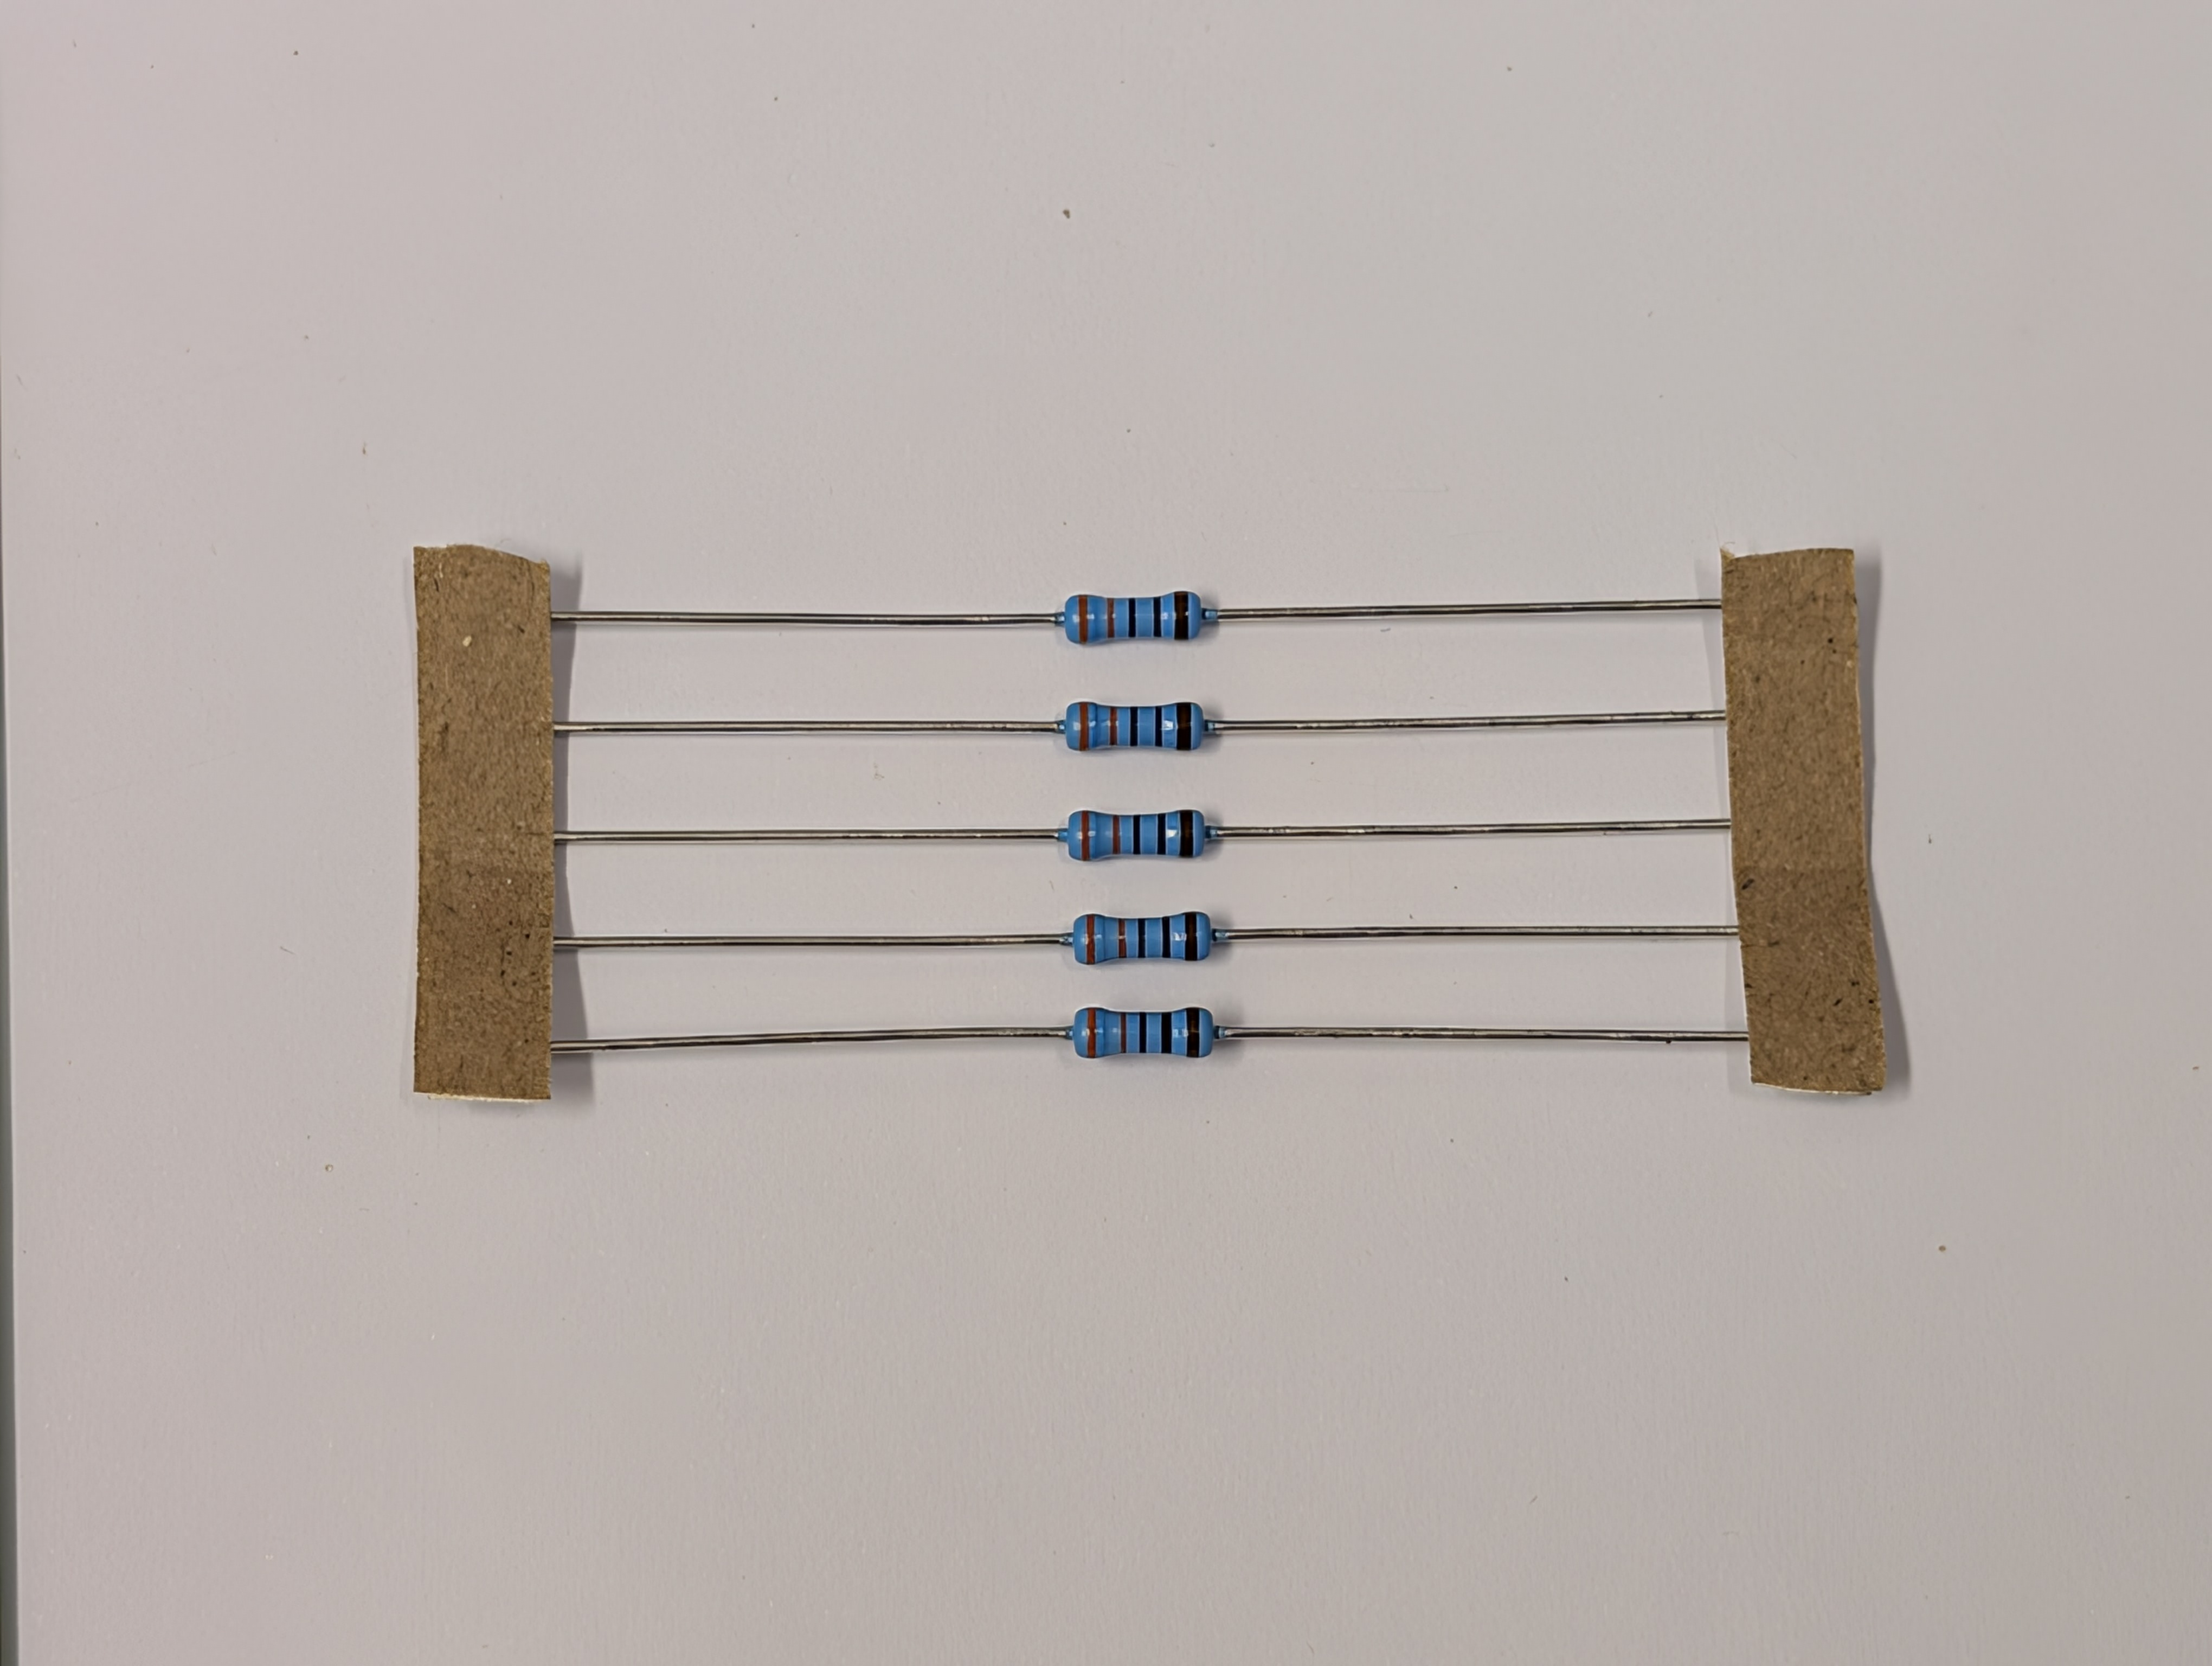
\includegraphics[width=0.75\textwidth]{pictures_of_construction/instruction_step_33.jpg}
\end{figure}

\begin{figure}[H]
    \centering
    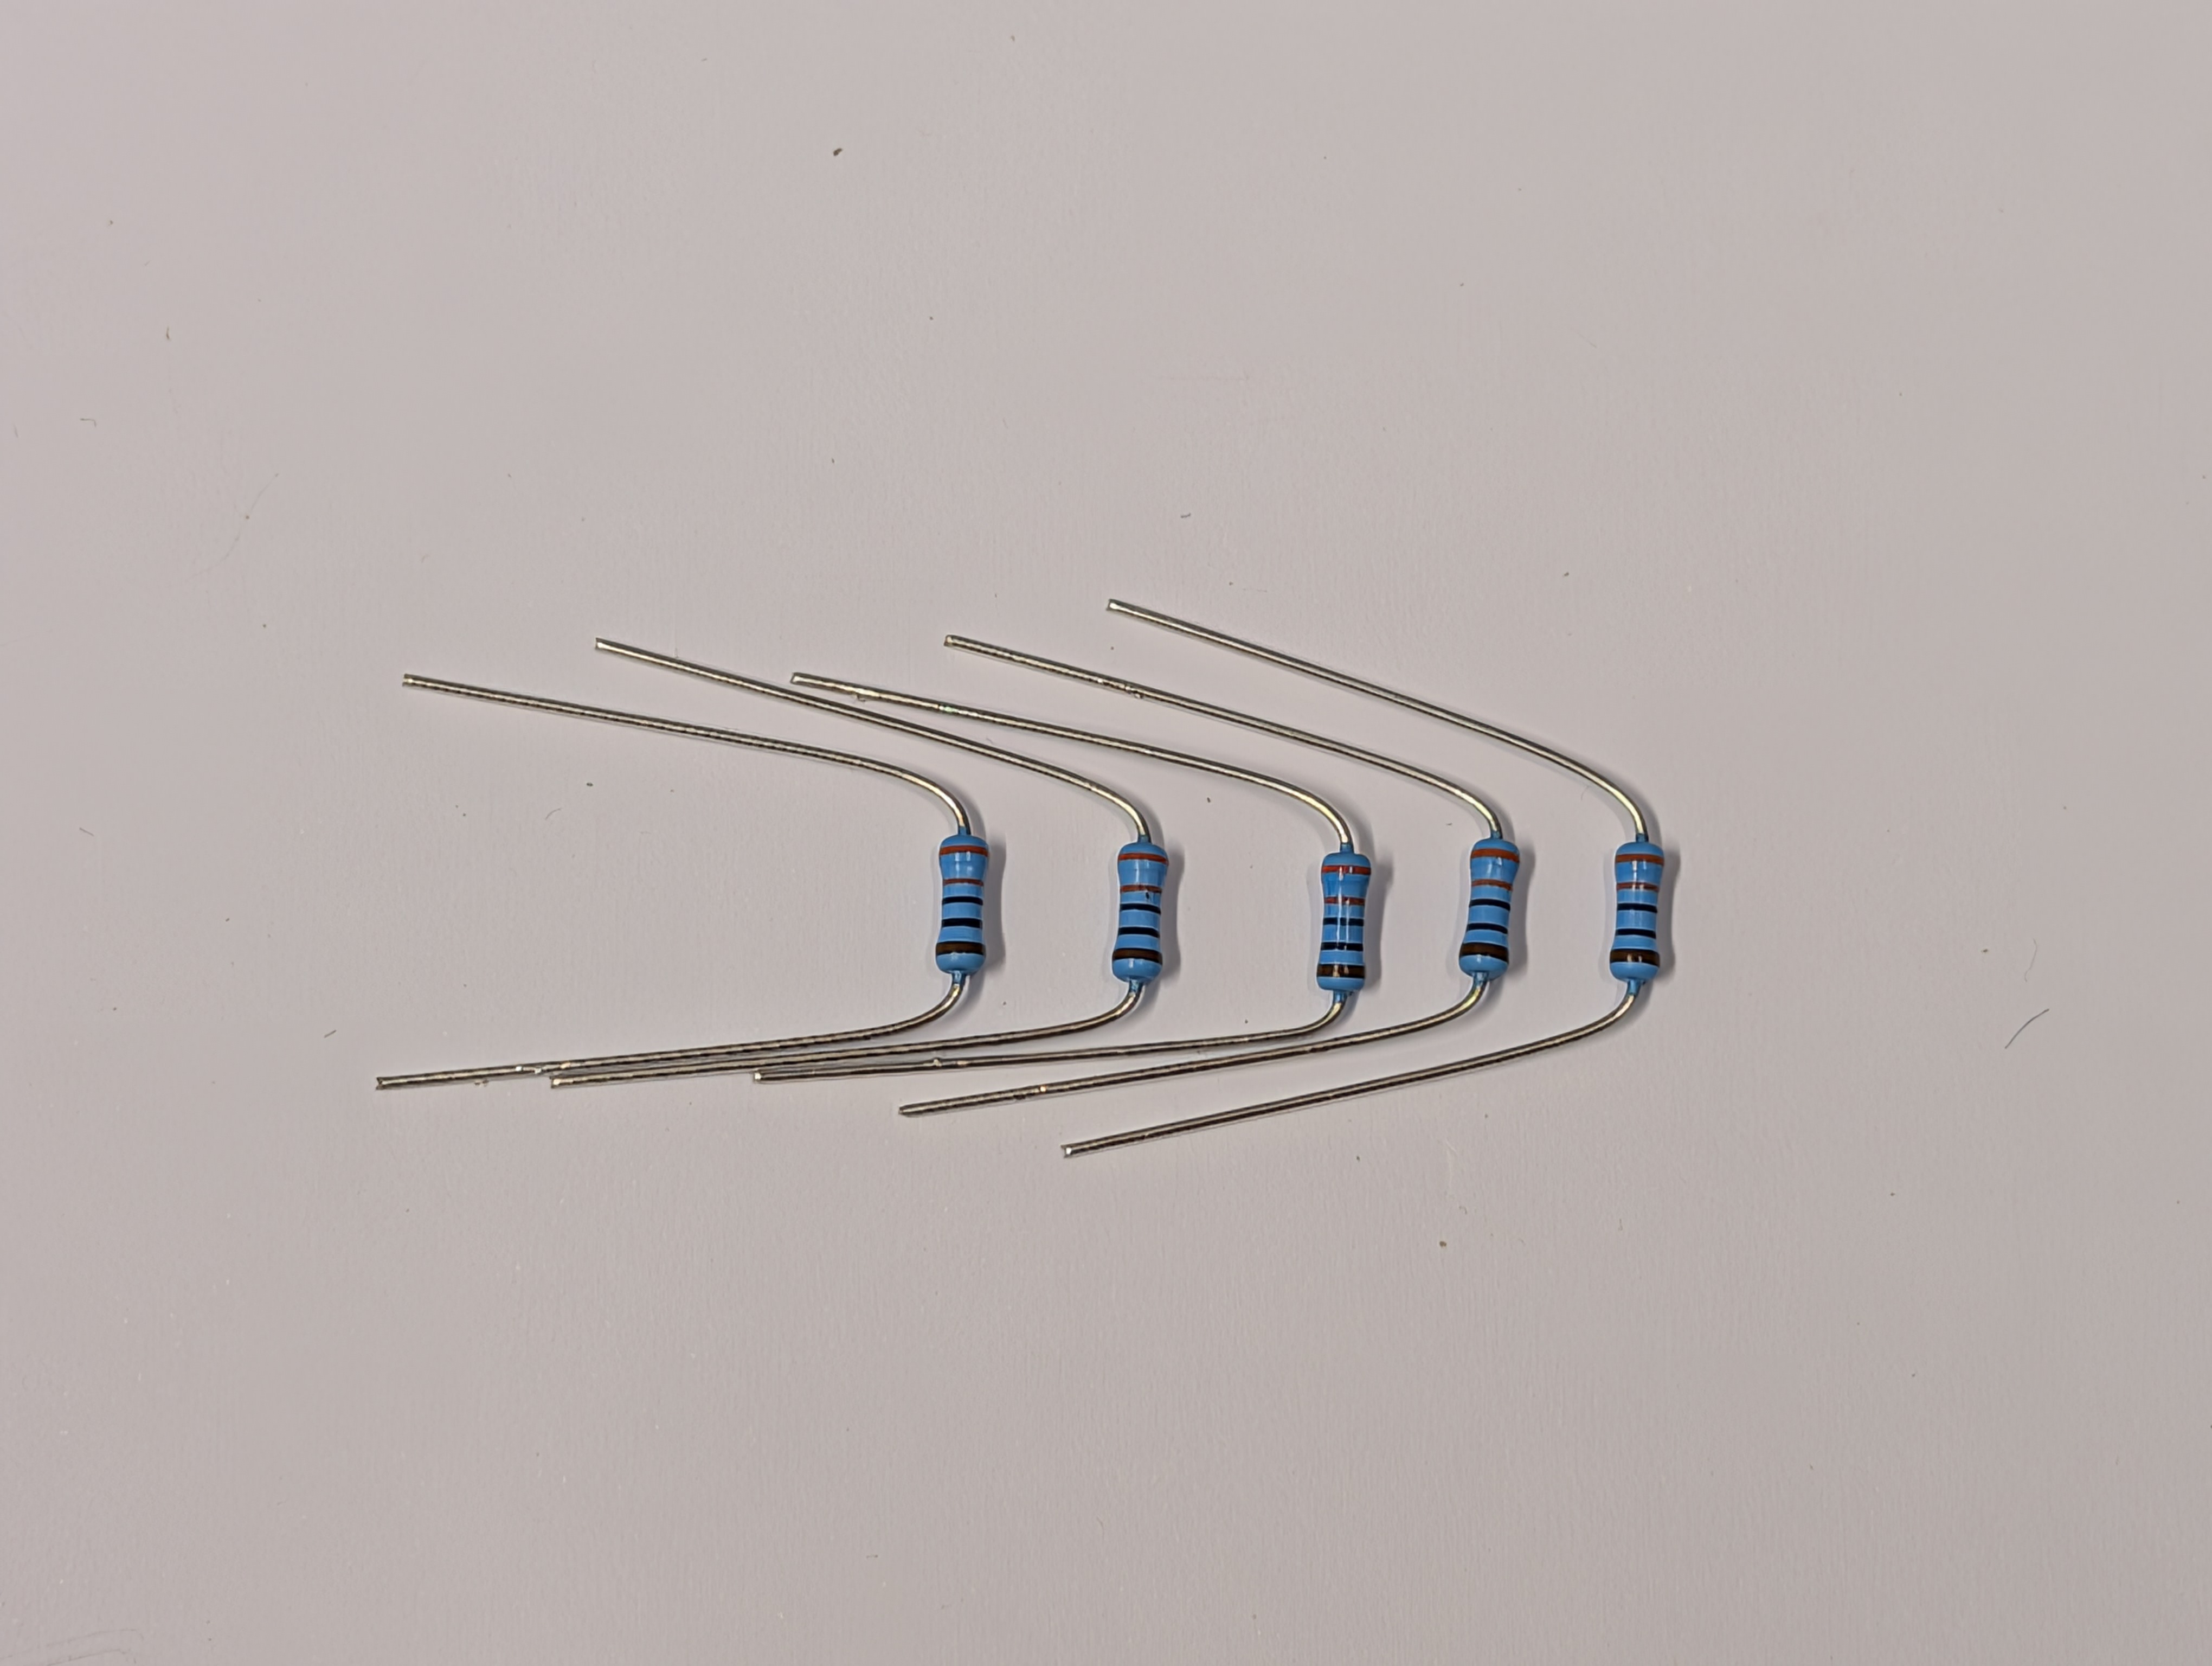
\includegraphics[width=0.75\textwidth]{pictures_of_construction/instruction_step_34.jpg}
\end{figure}

\begin{figure}[H]
    \centering
    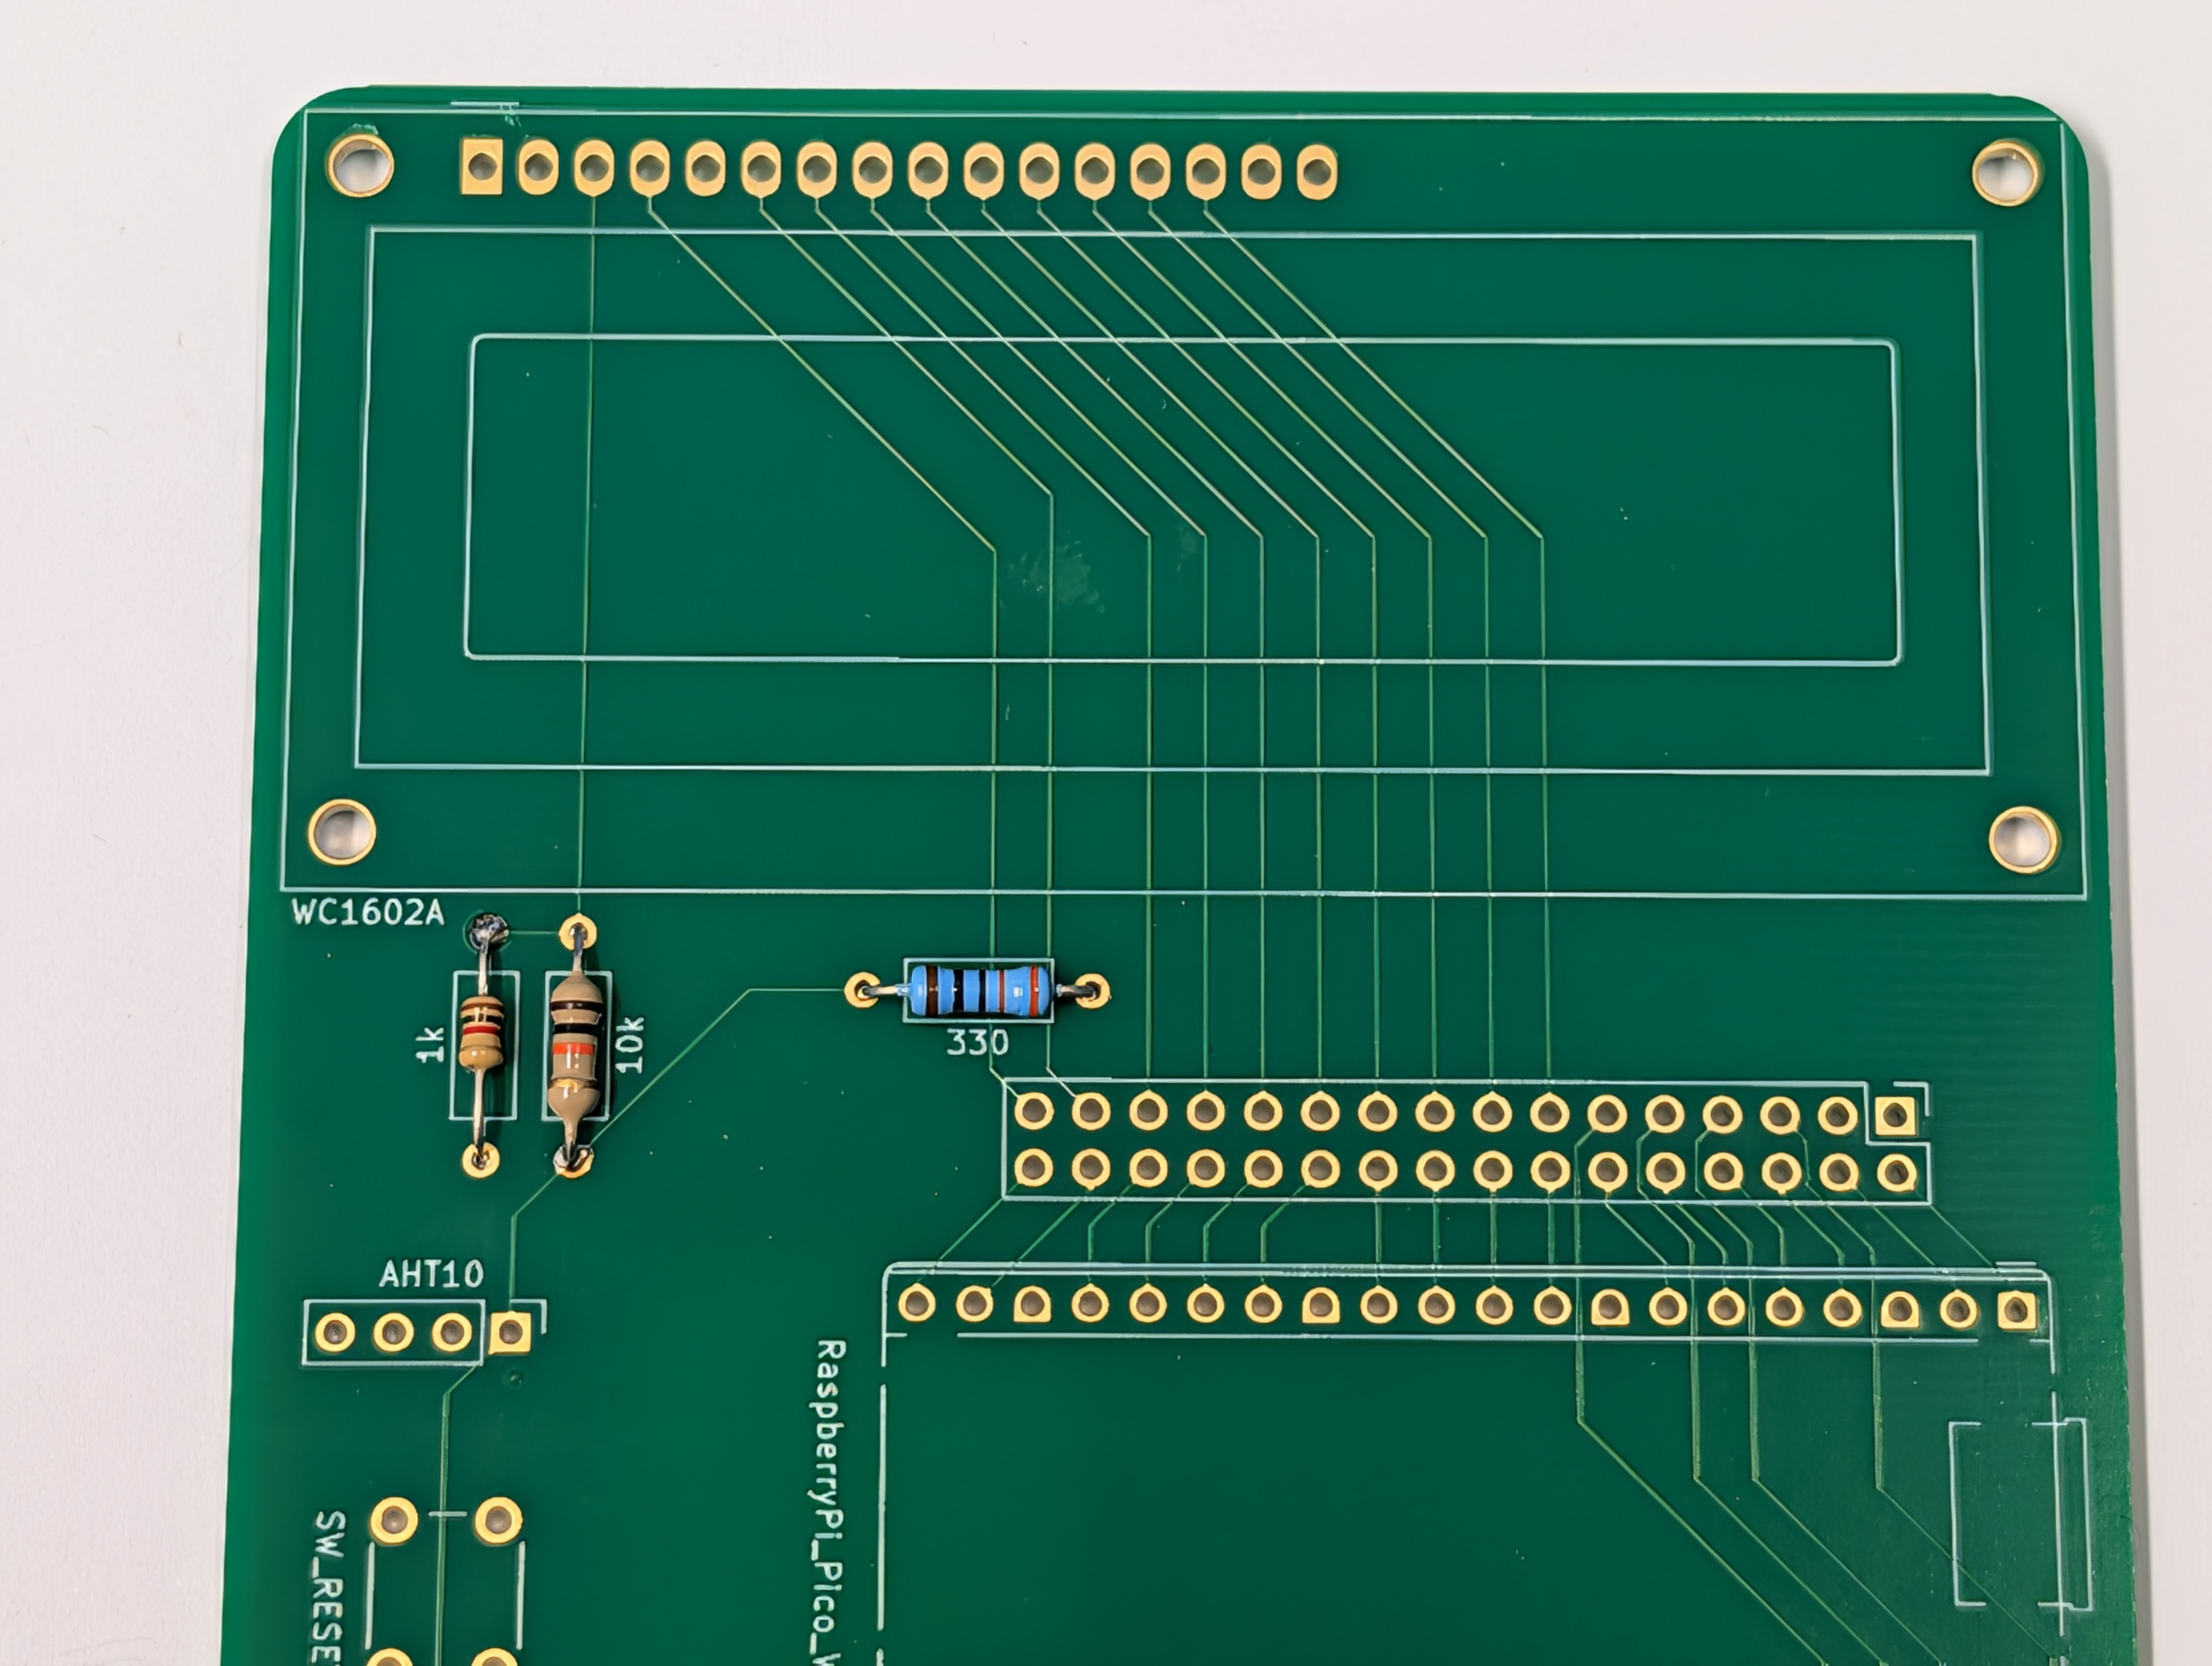
\includegraphics[width=0.75\textwidth]{pictures_of_construction/instruction_step_35.jpg}
\end{figure}

\begin{figure}[H]
    \centering
    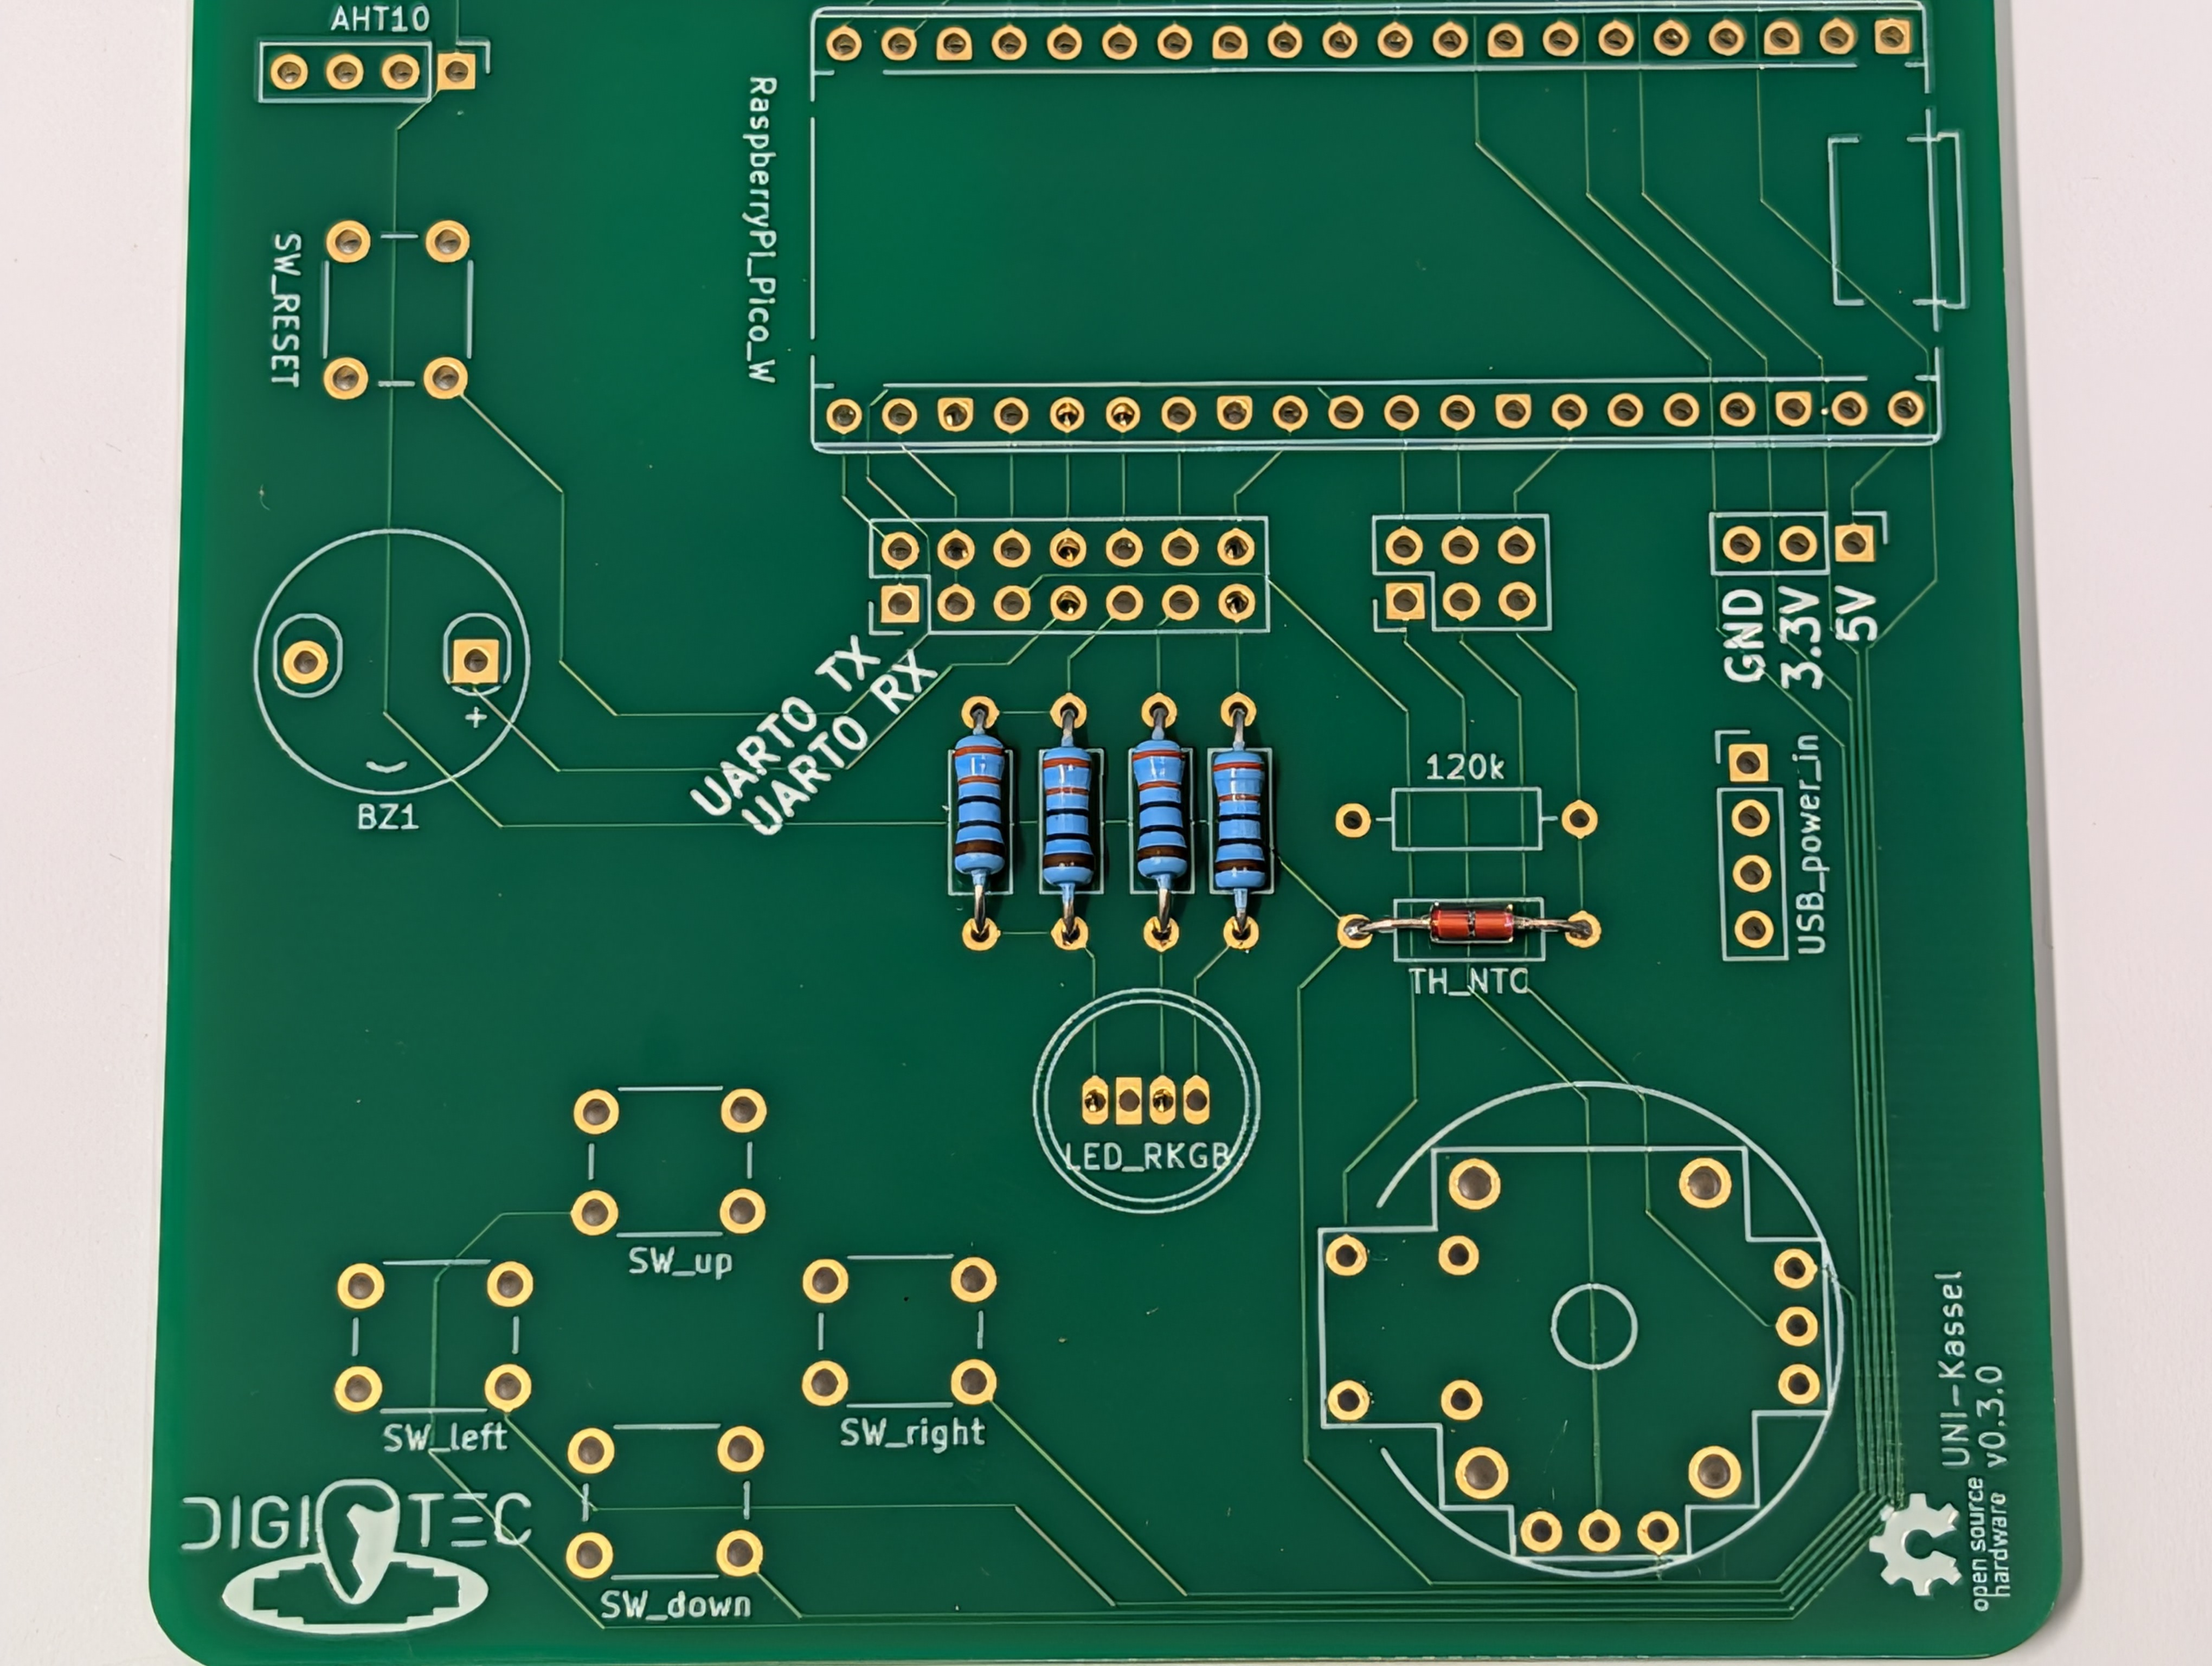
\includegraphics[width=0.75\textwidth]{pictures_of_construction/instruction_step_36.jpg}
\end{figure}

\subsubsection*{5e. 120-k$\Omega$-Widerstand einbauen}

Farbringe:
\begin{itemize}
    \item Braun
    \item Rot
    \item Gelb
    \item Gold
\end{itemize}

Auch diesen wie die anderen Widerstände einbauen.

\begin{figure}[H]
    \centering
    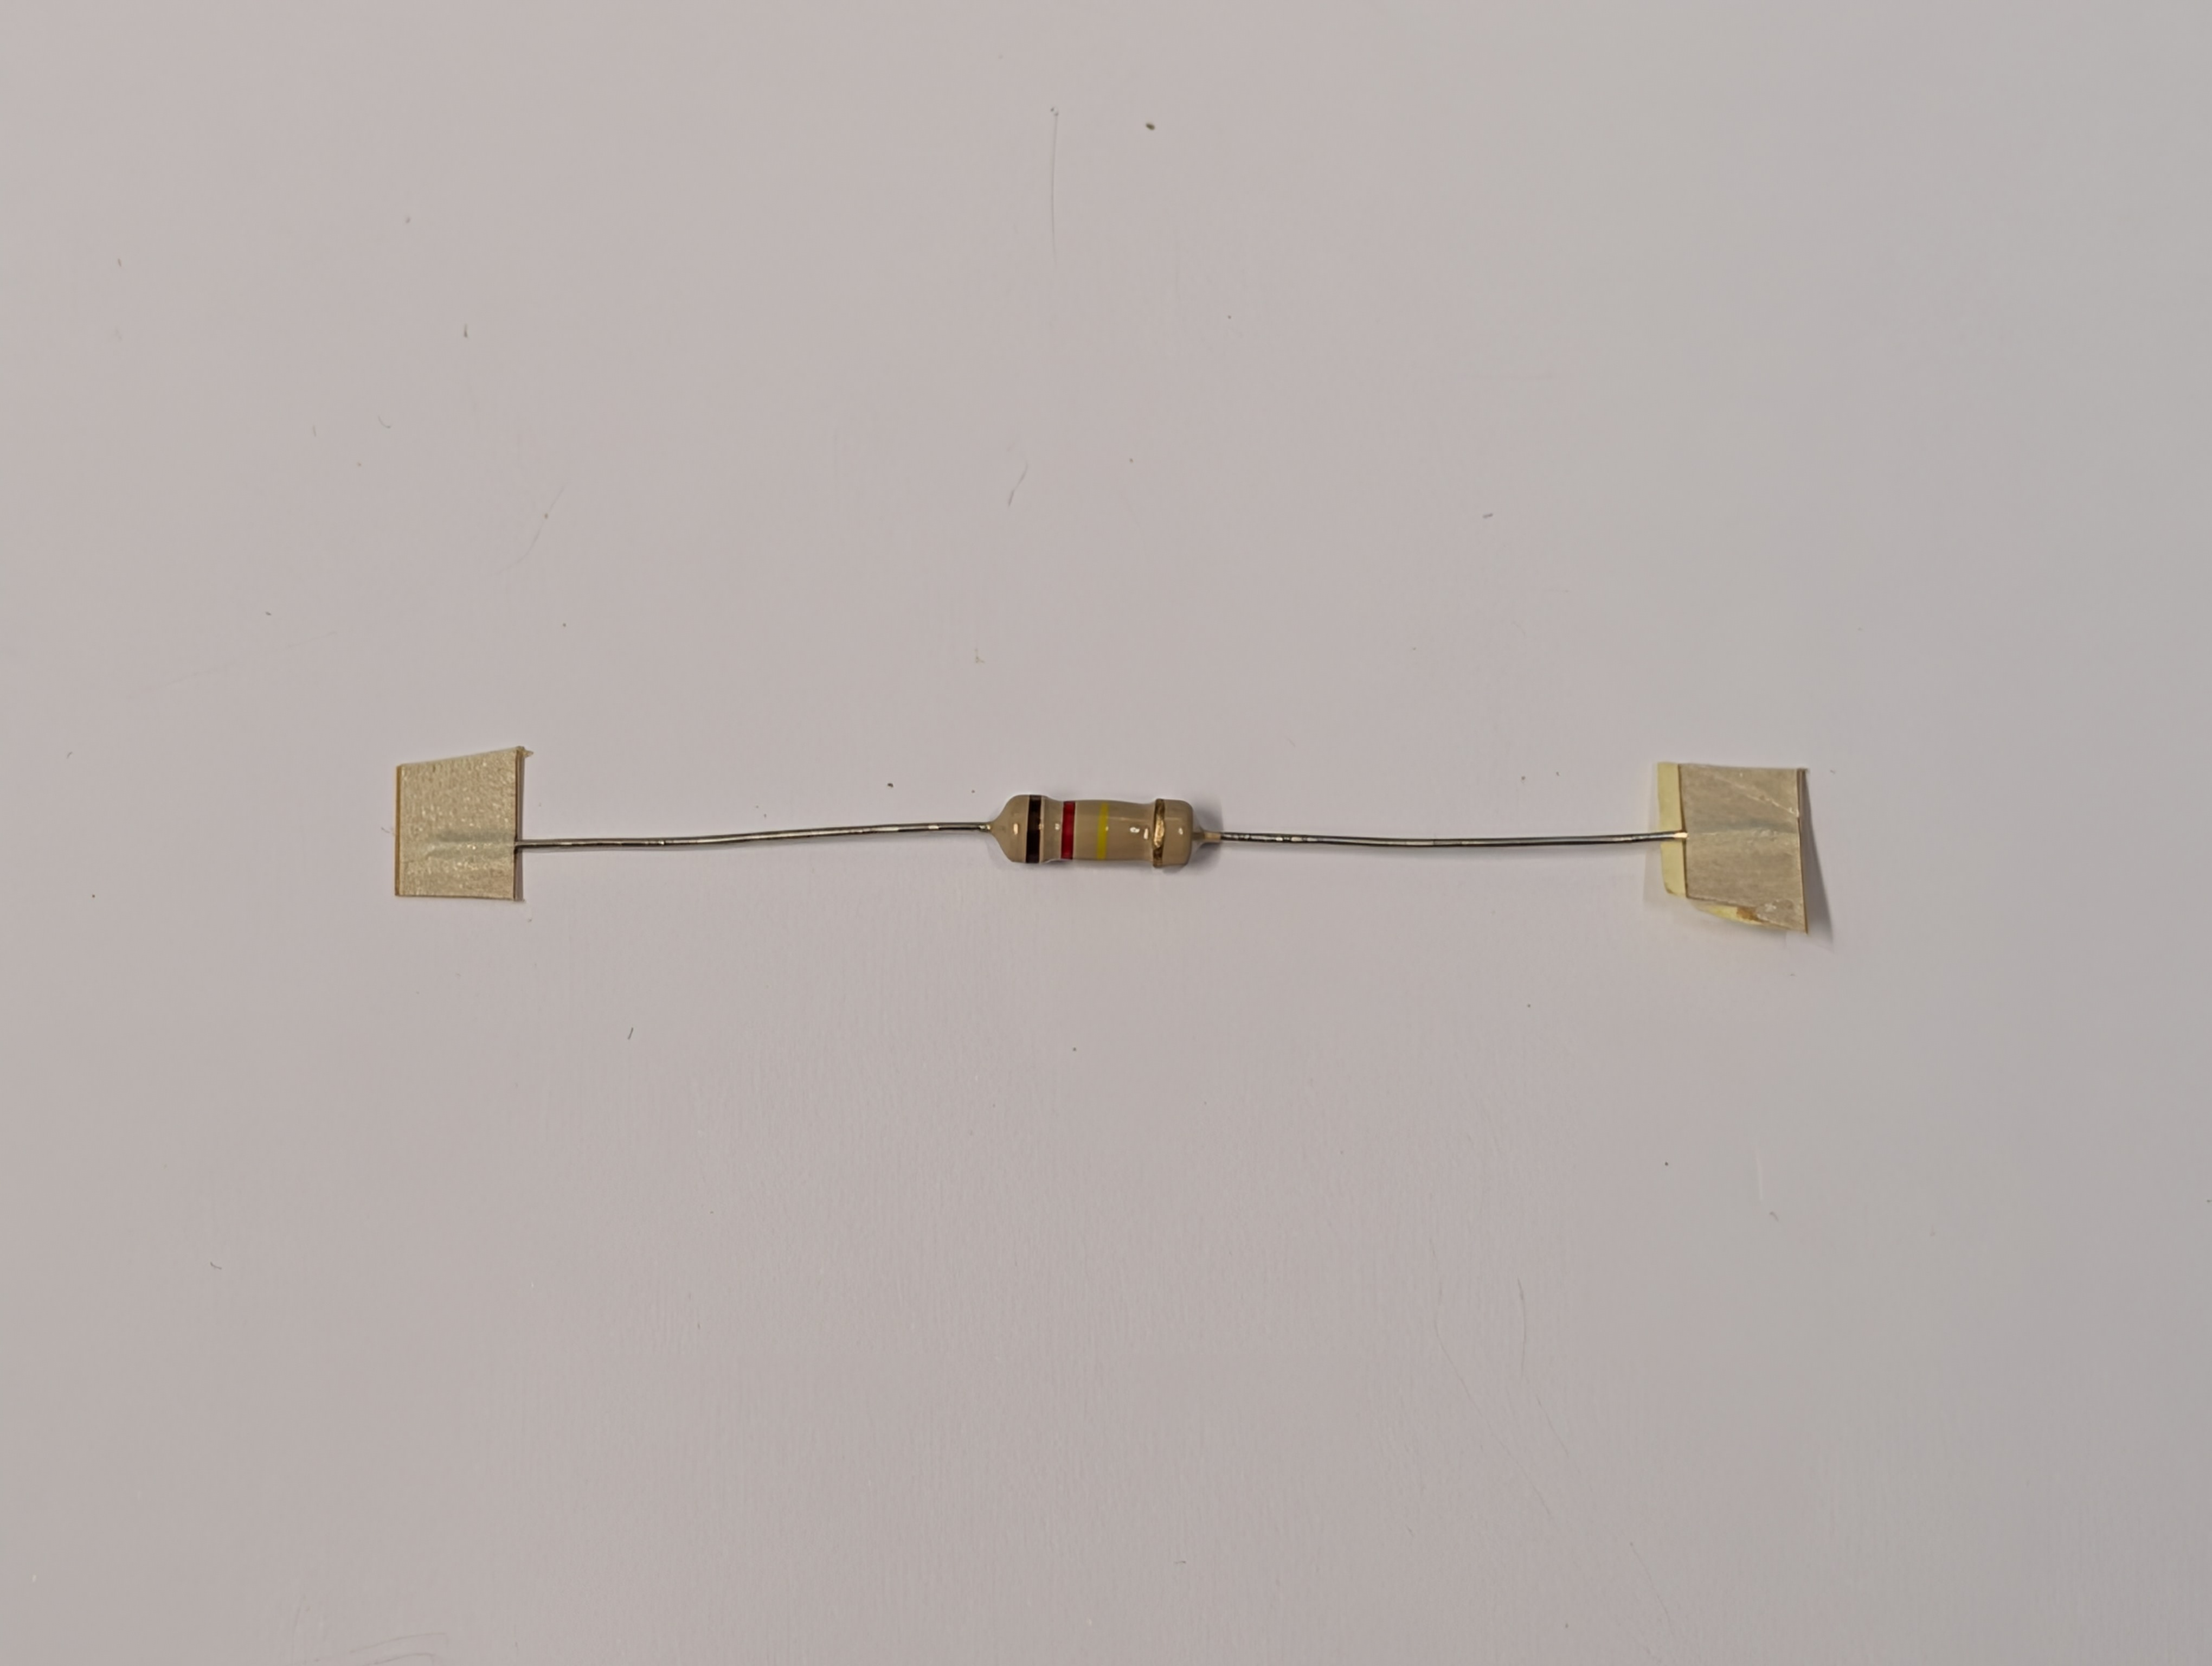
\includegraphics[width=0.75\textwidth]{pictures_of_construction/instruction_step_37.jpg}
\end{figure}

\begin{figure}[H]
    \centering
    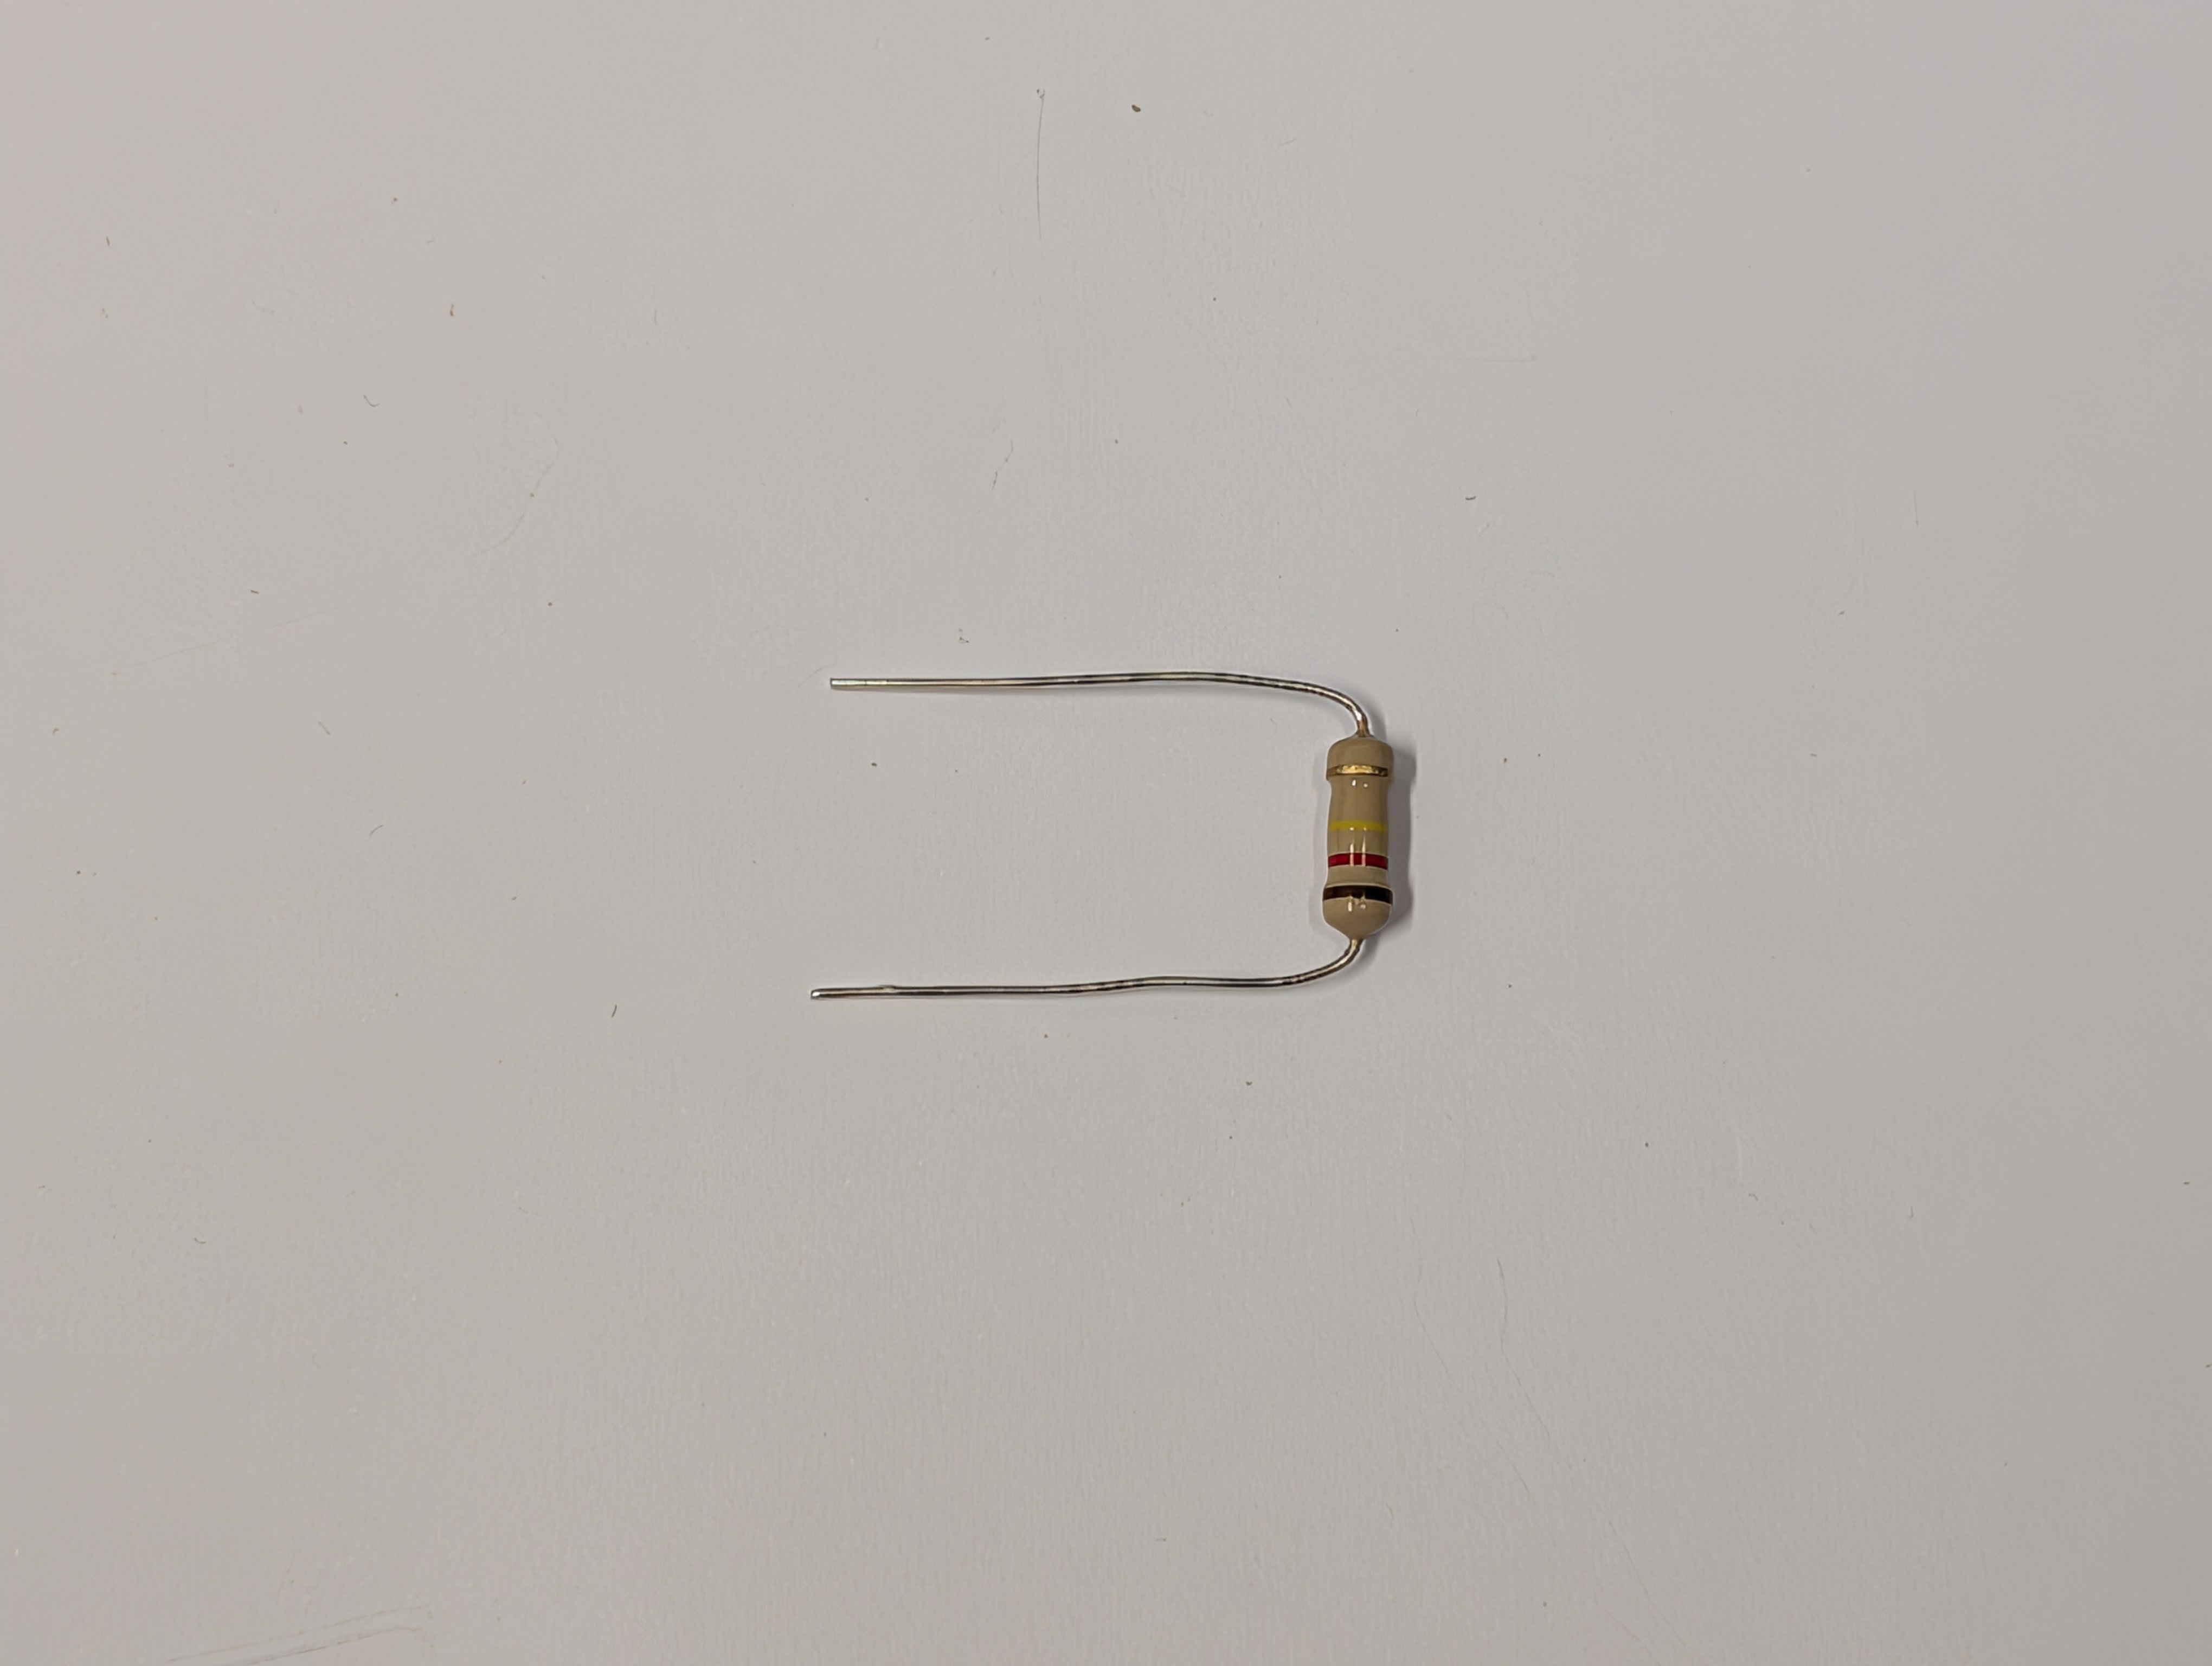
\includegraphics[width=0.75\textwidth]{pictures_of_construction/instruction_step_38.jpg}
\end{figure}

\begin{figure}[H]
    \centering
    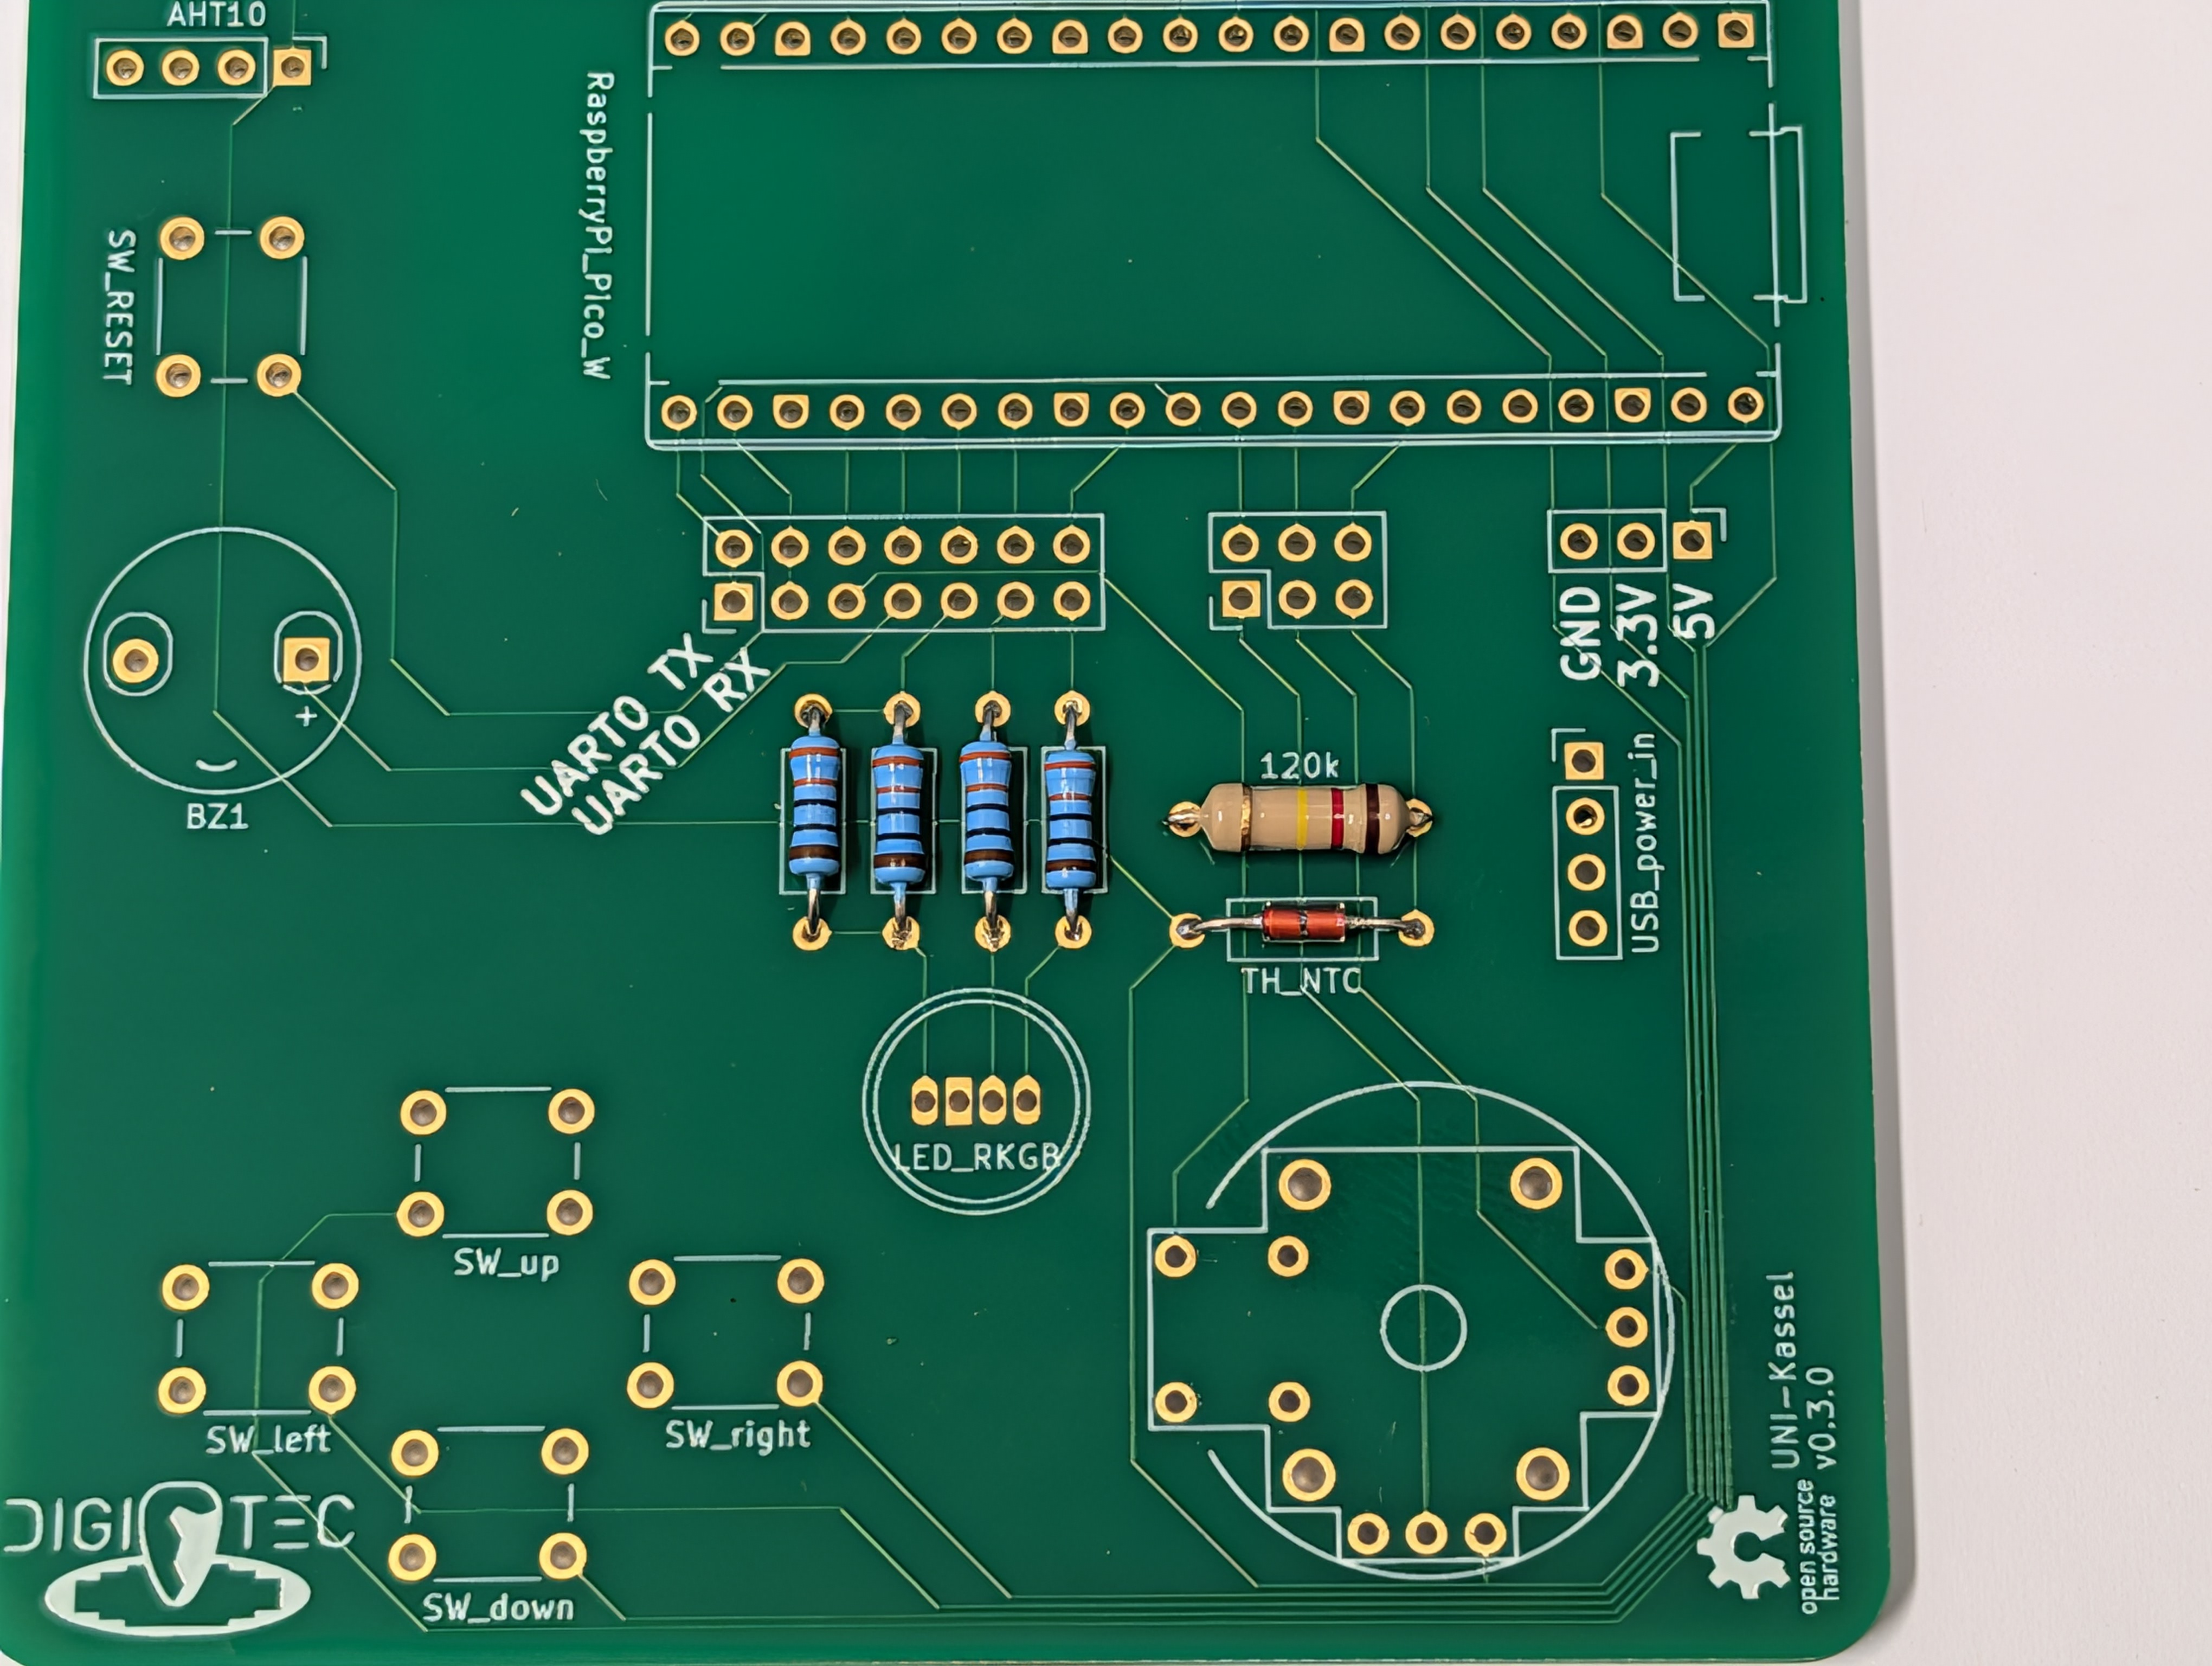
\includegraphics[width=0.75\textwidth]{pictures_of_construction/instruction_step_39.jpg}
\end{figure}

\subsection*{6. Taster einbauen}

Jetzt kommen die fünf Taster auf die Platine.

So gehst du vor:
\begin{enumerate}
    \item Stecke einen Taster in die richtige Position.
    \item Drücke ihn ganz hinein, damit er flach auf der Platine sitzt.
    \item Löte die Pins fest.
    \item Wiederhole das mit den anderen Tastern.
\end{enumerate}

Es gibt:
\begin{itemize}
    \item einen Reset-Taster
    \item vier D-Pad-Taster
\end{itemize}

\textbf{Wichtig:}
Die Taster sollen \textbf{möglichst flach} auf der Platine sitzen.

\begin{figure}[H]
    \centering
    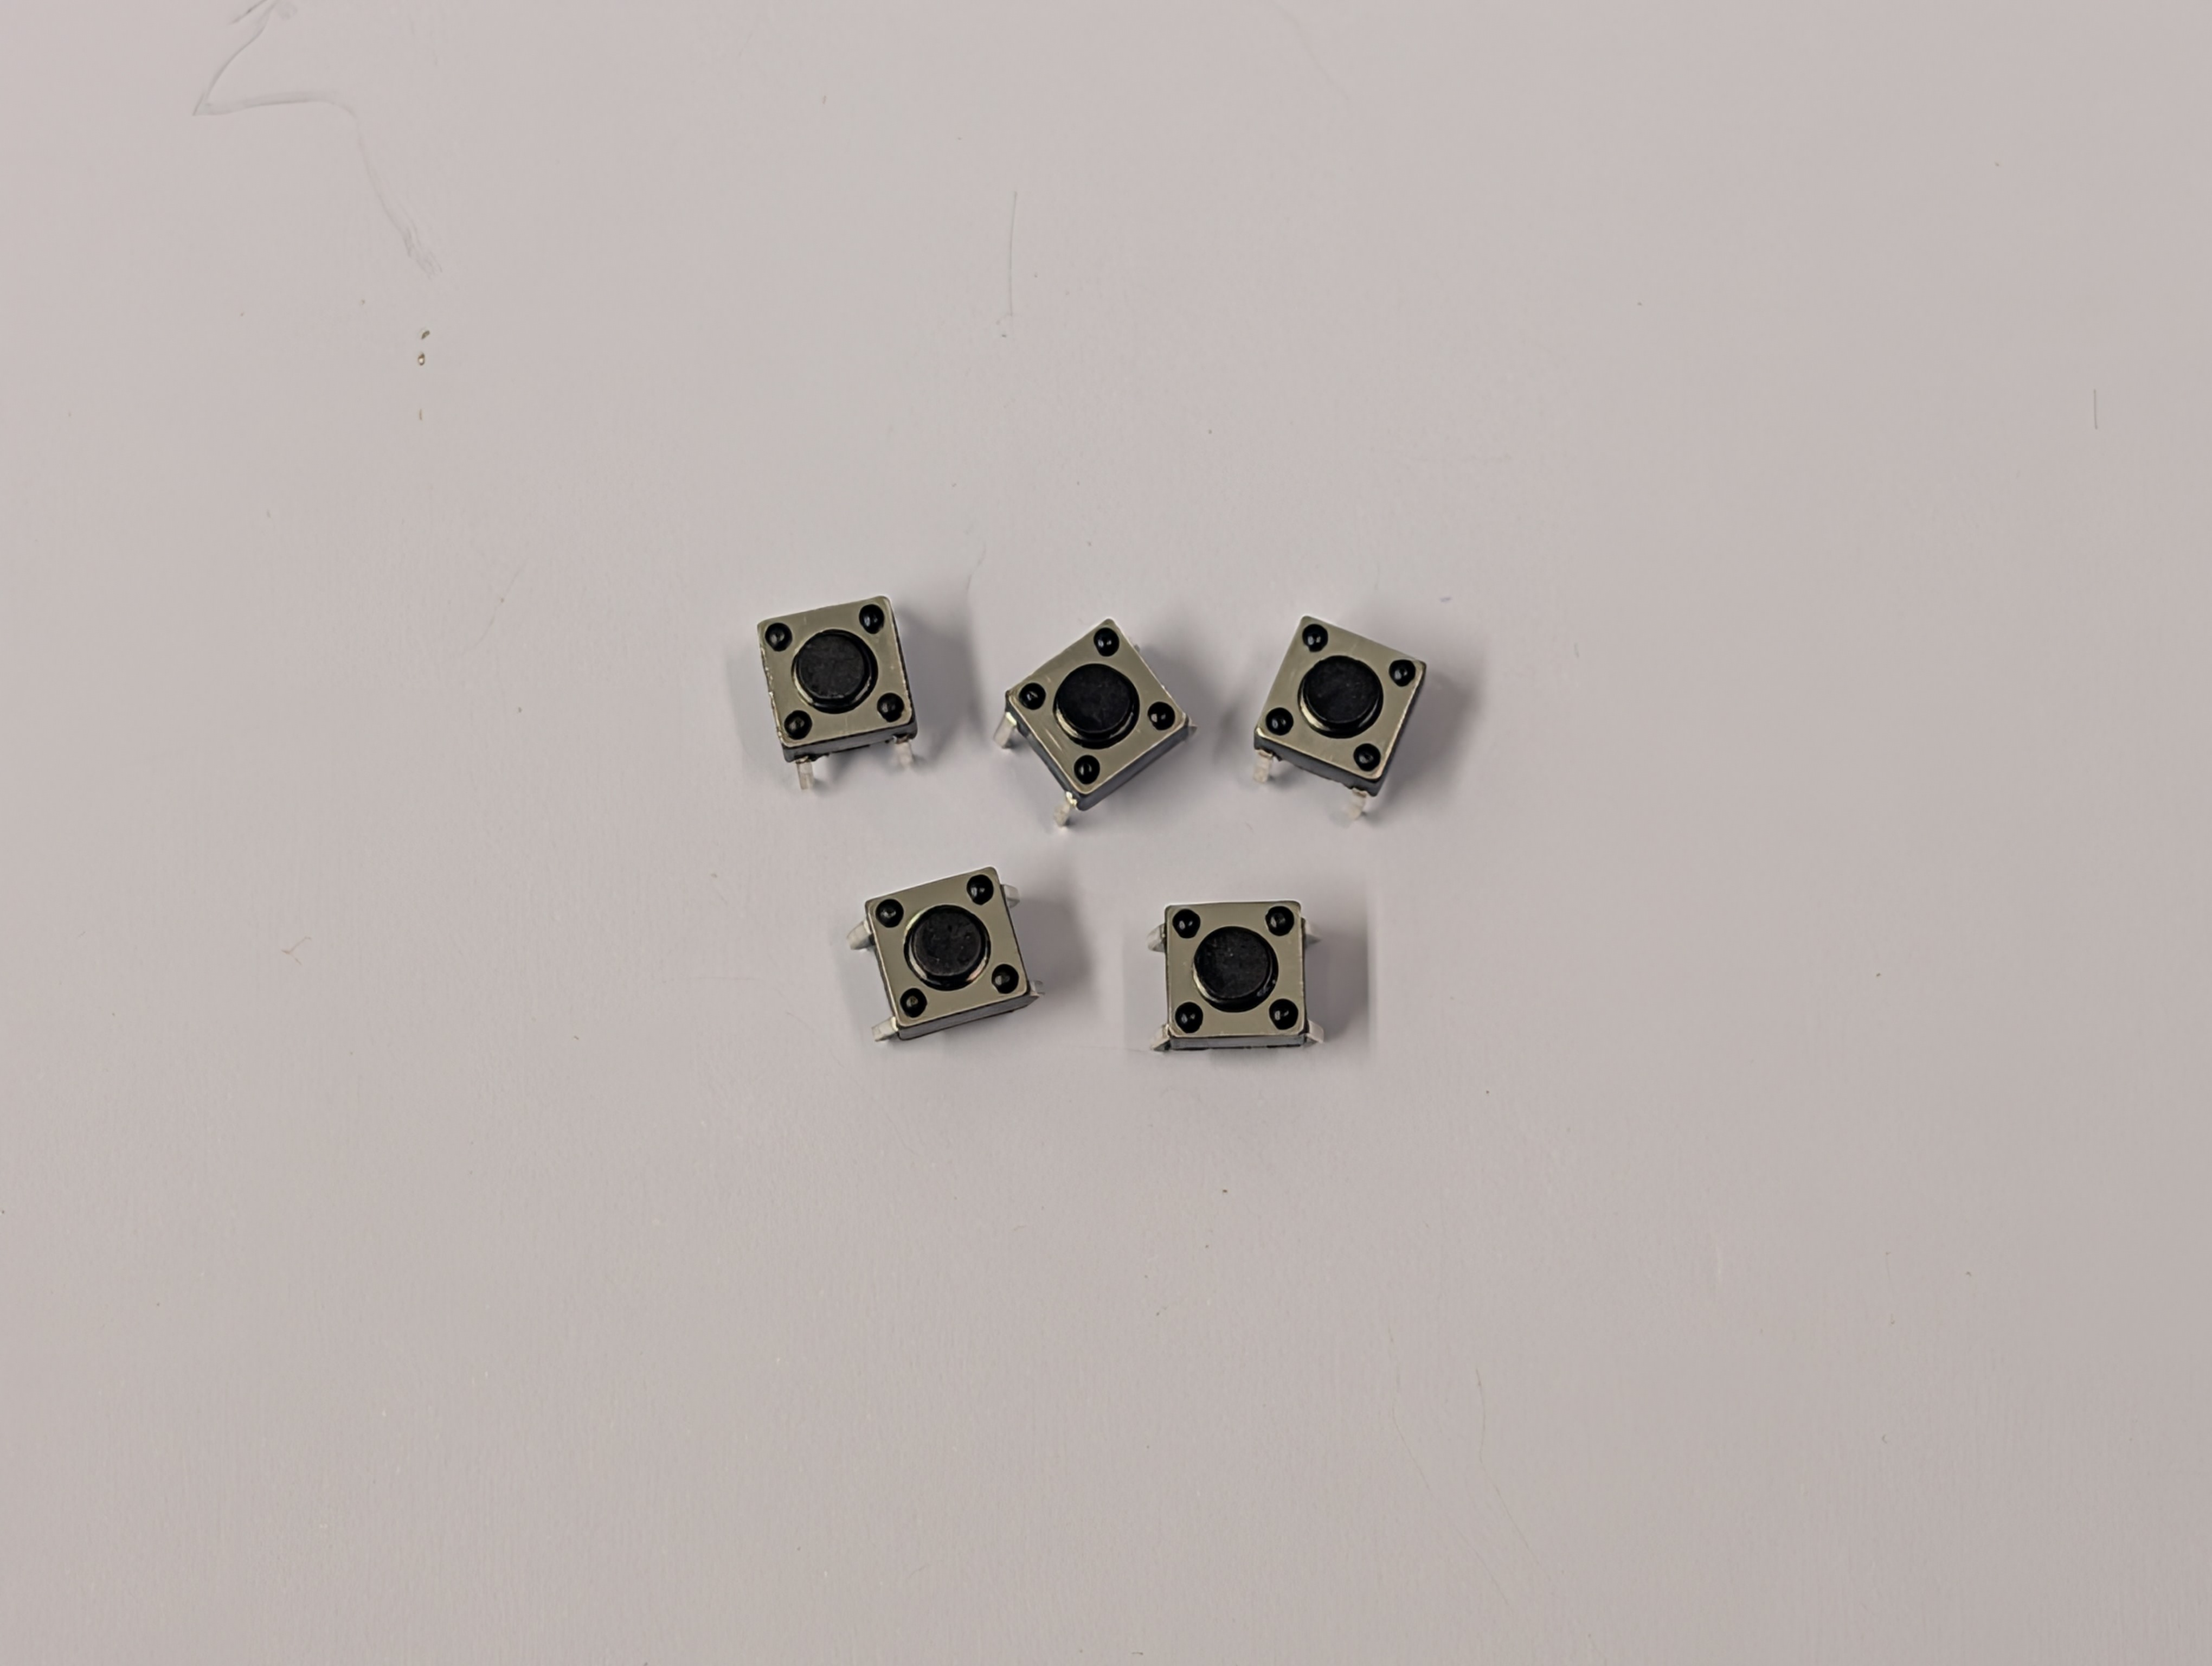
\includegraphics[width=0.75\textwidth]{pictures_of_construction/instruction_step_40.jpg}
\end{figure}

\begin{figure}[H]
    \centering
    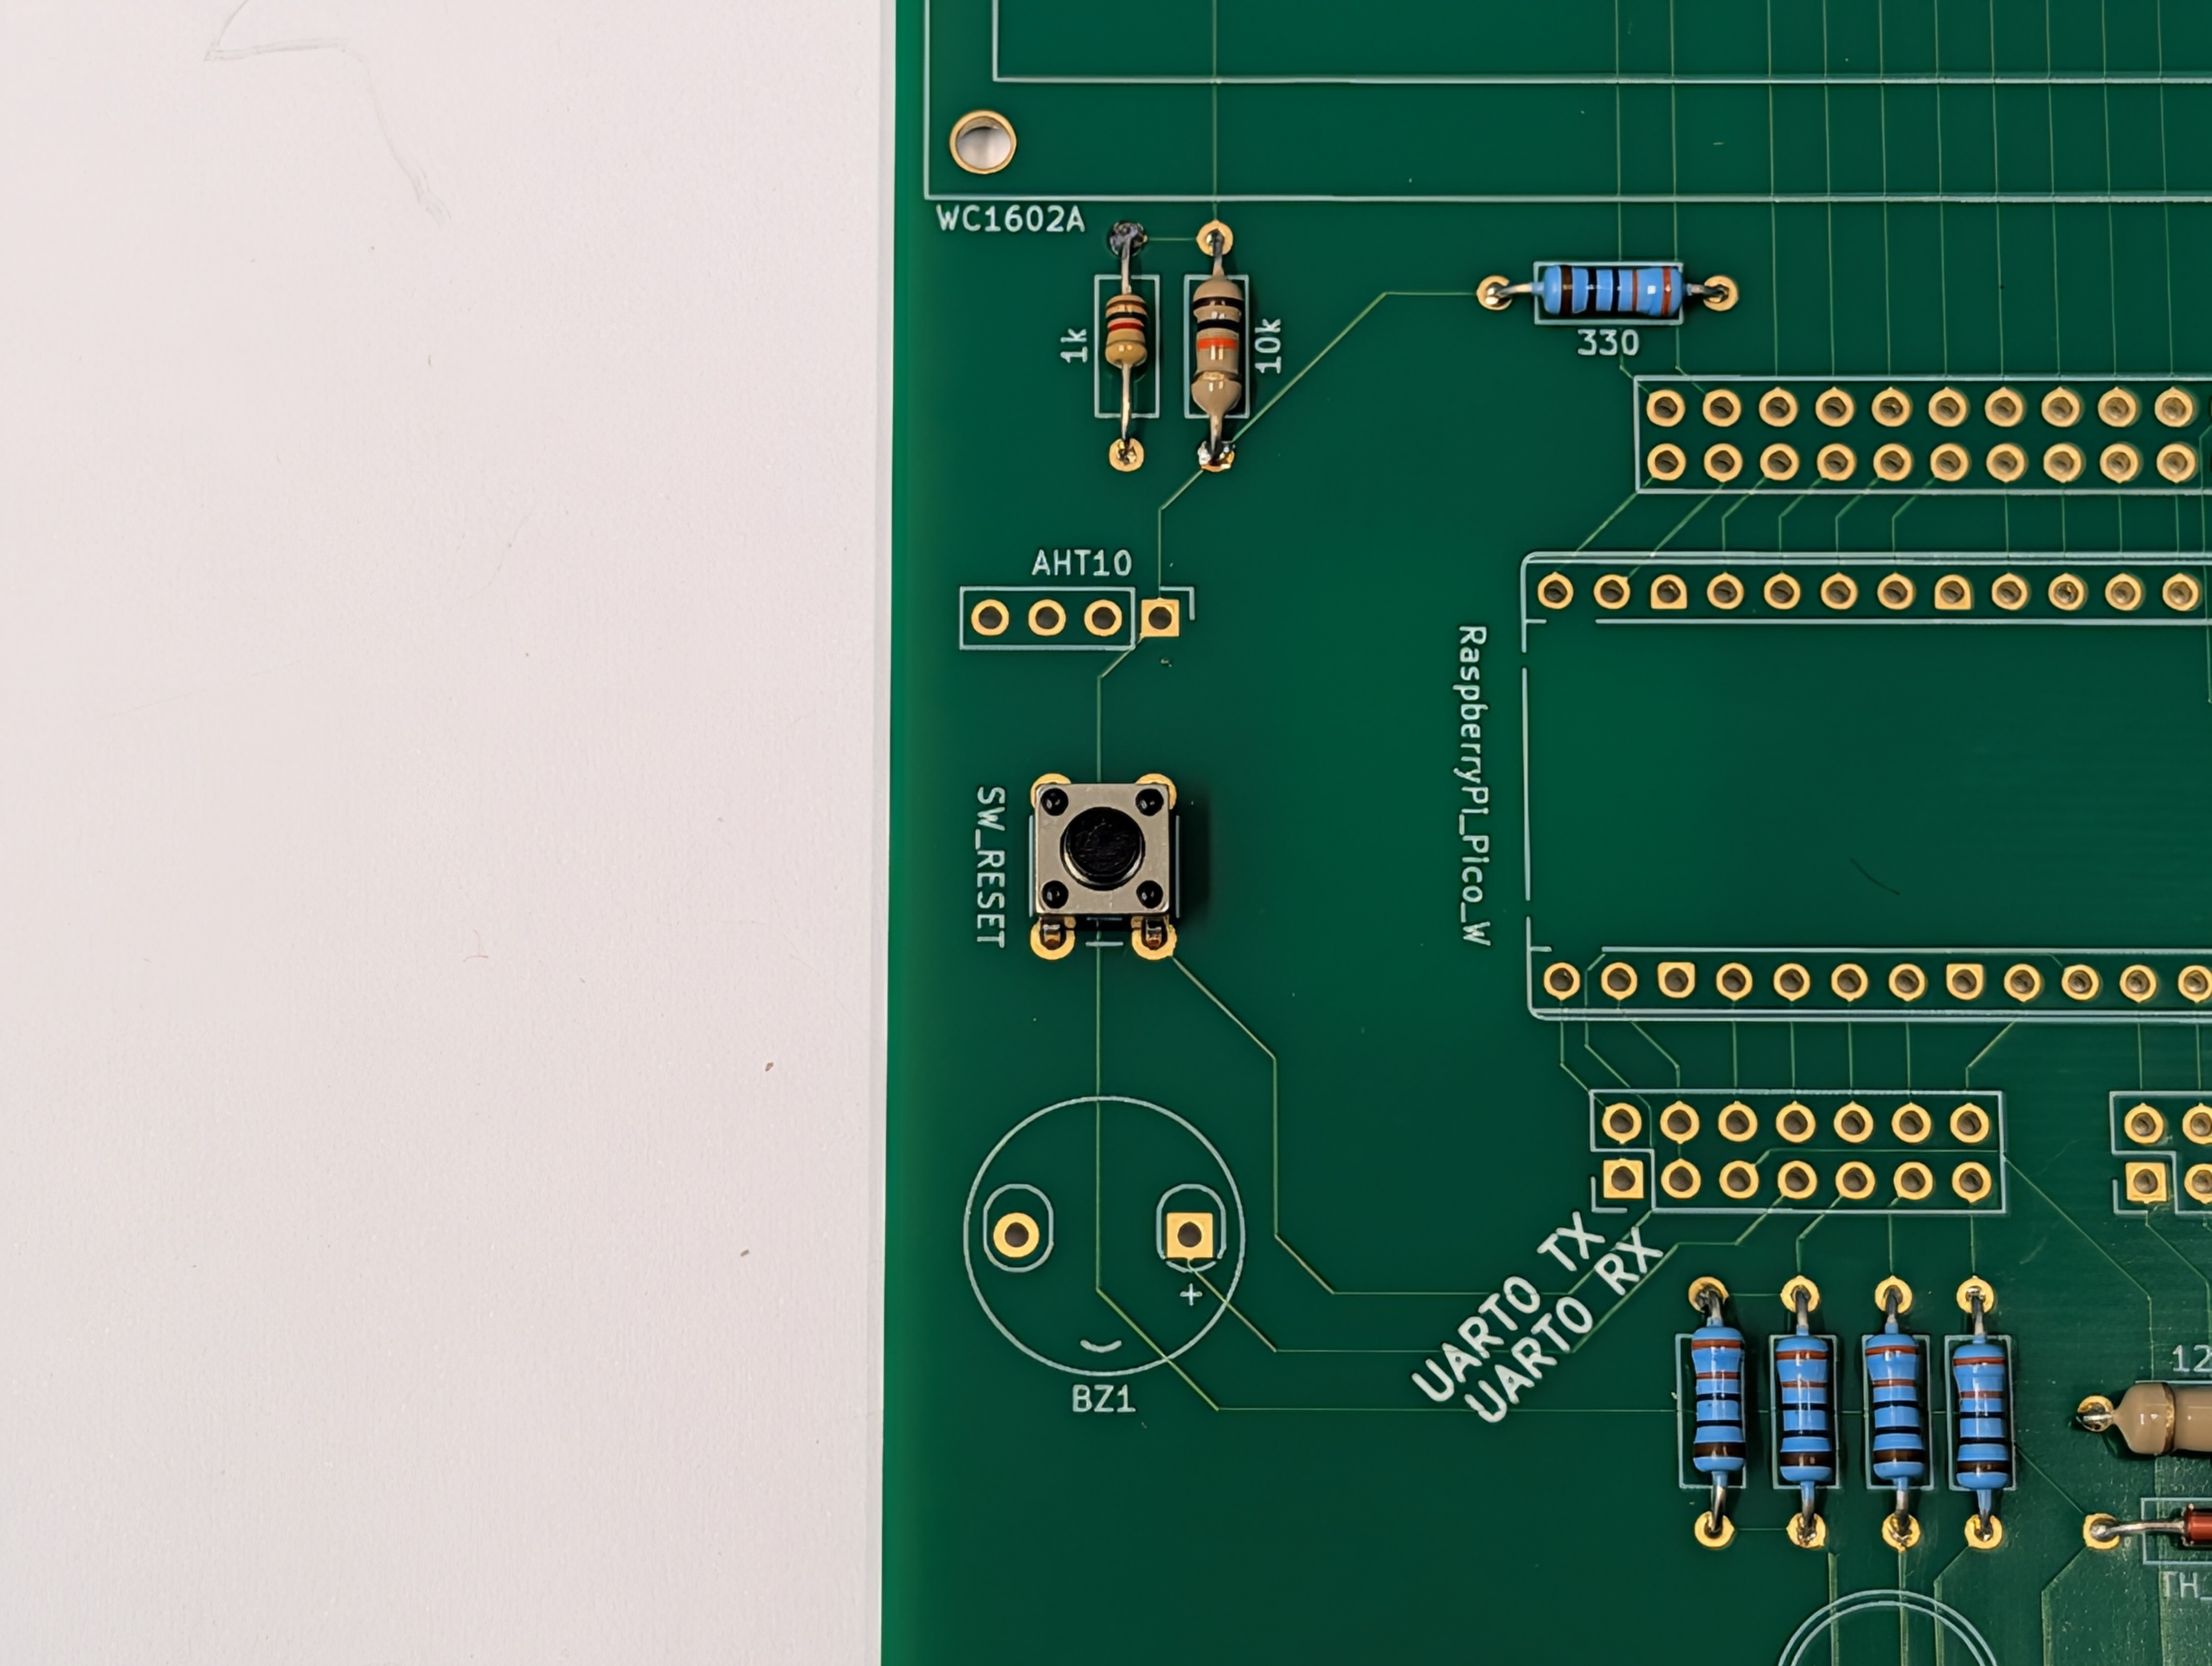
\includegraphics[width=0.75\textwidth]{pictures_of_construction/instruction_step_41.jpg}
\end{figure}

\begin{figure}[H]
    \centering
    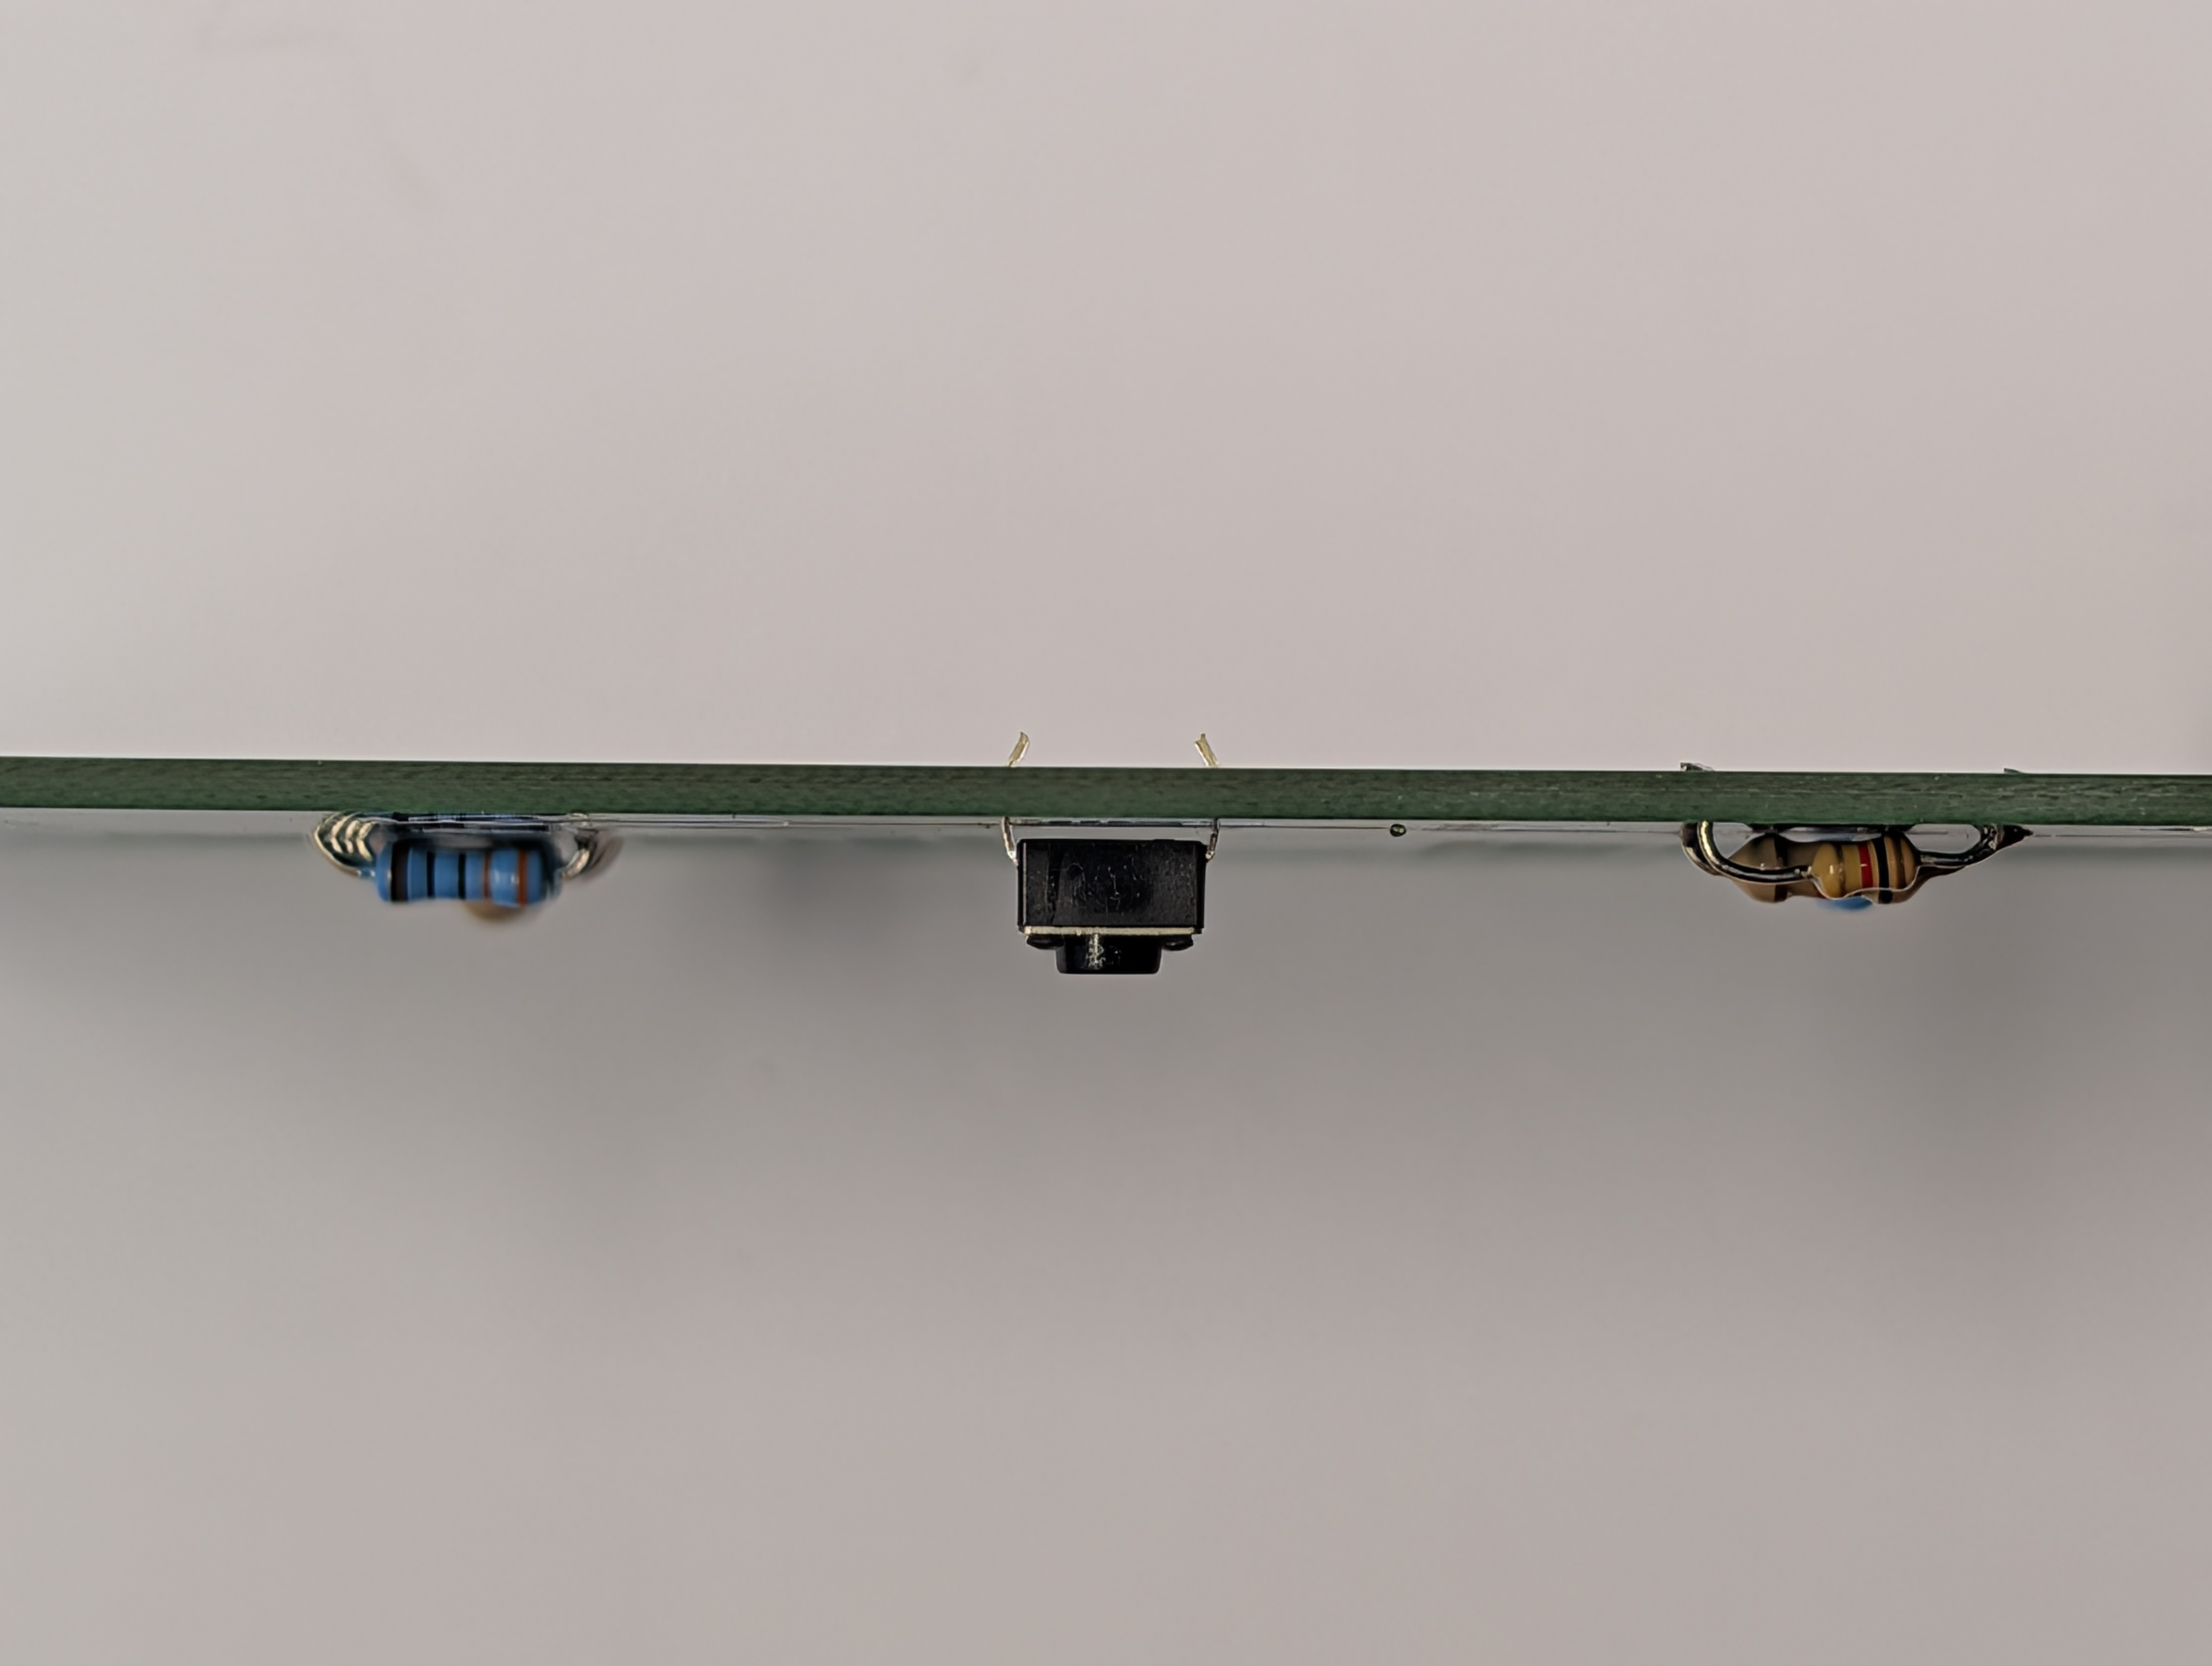
\includegraphics[width=0.75\textwidth]{pictures_of_construction/instruction_step_42.jpg}
\end{figure}

\begin{figure}[H]
    \centering
    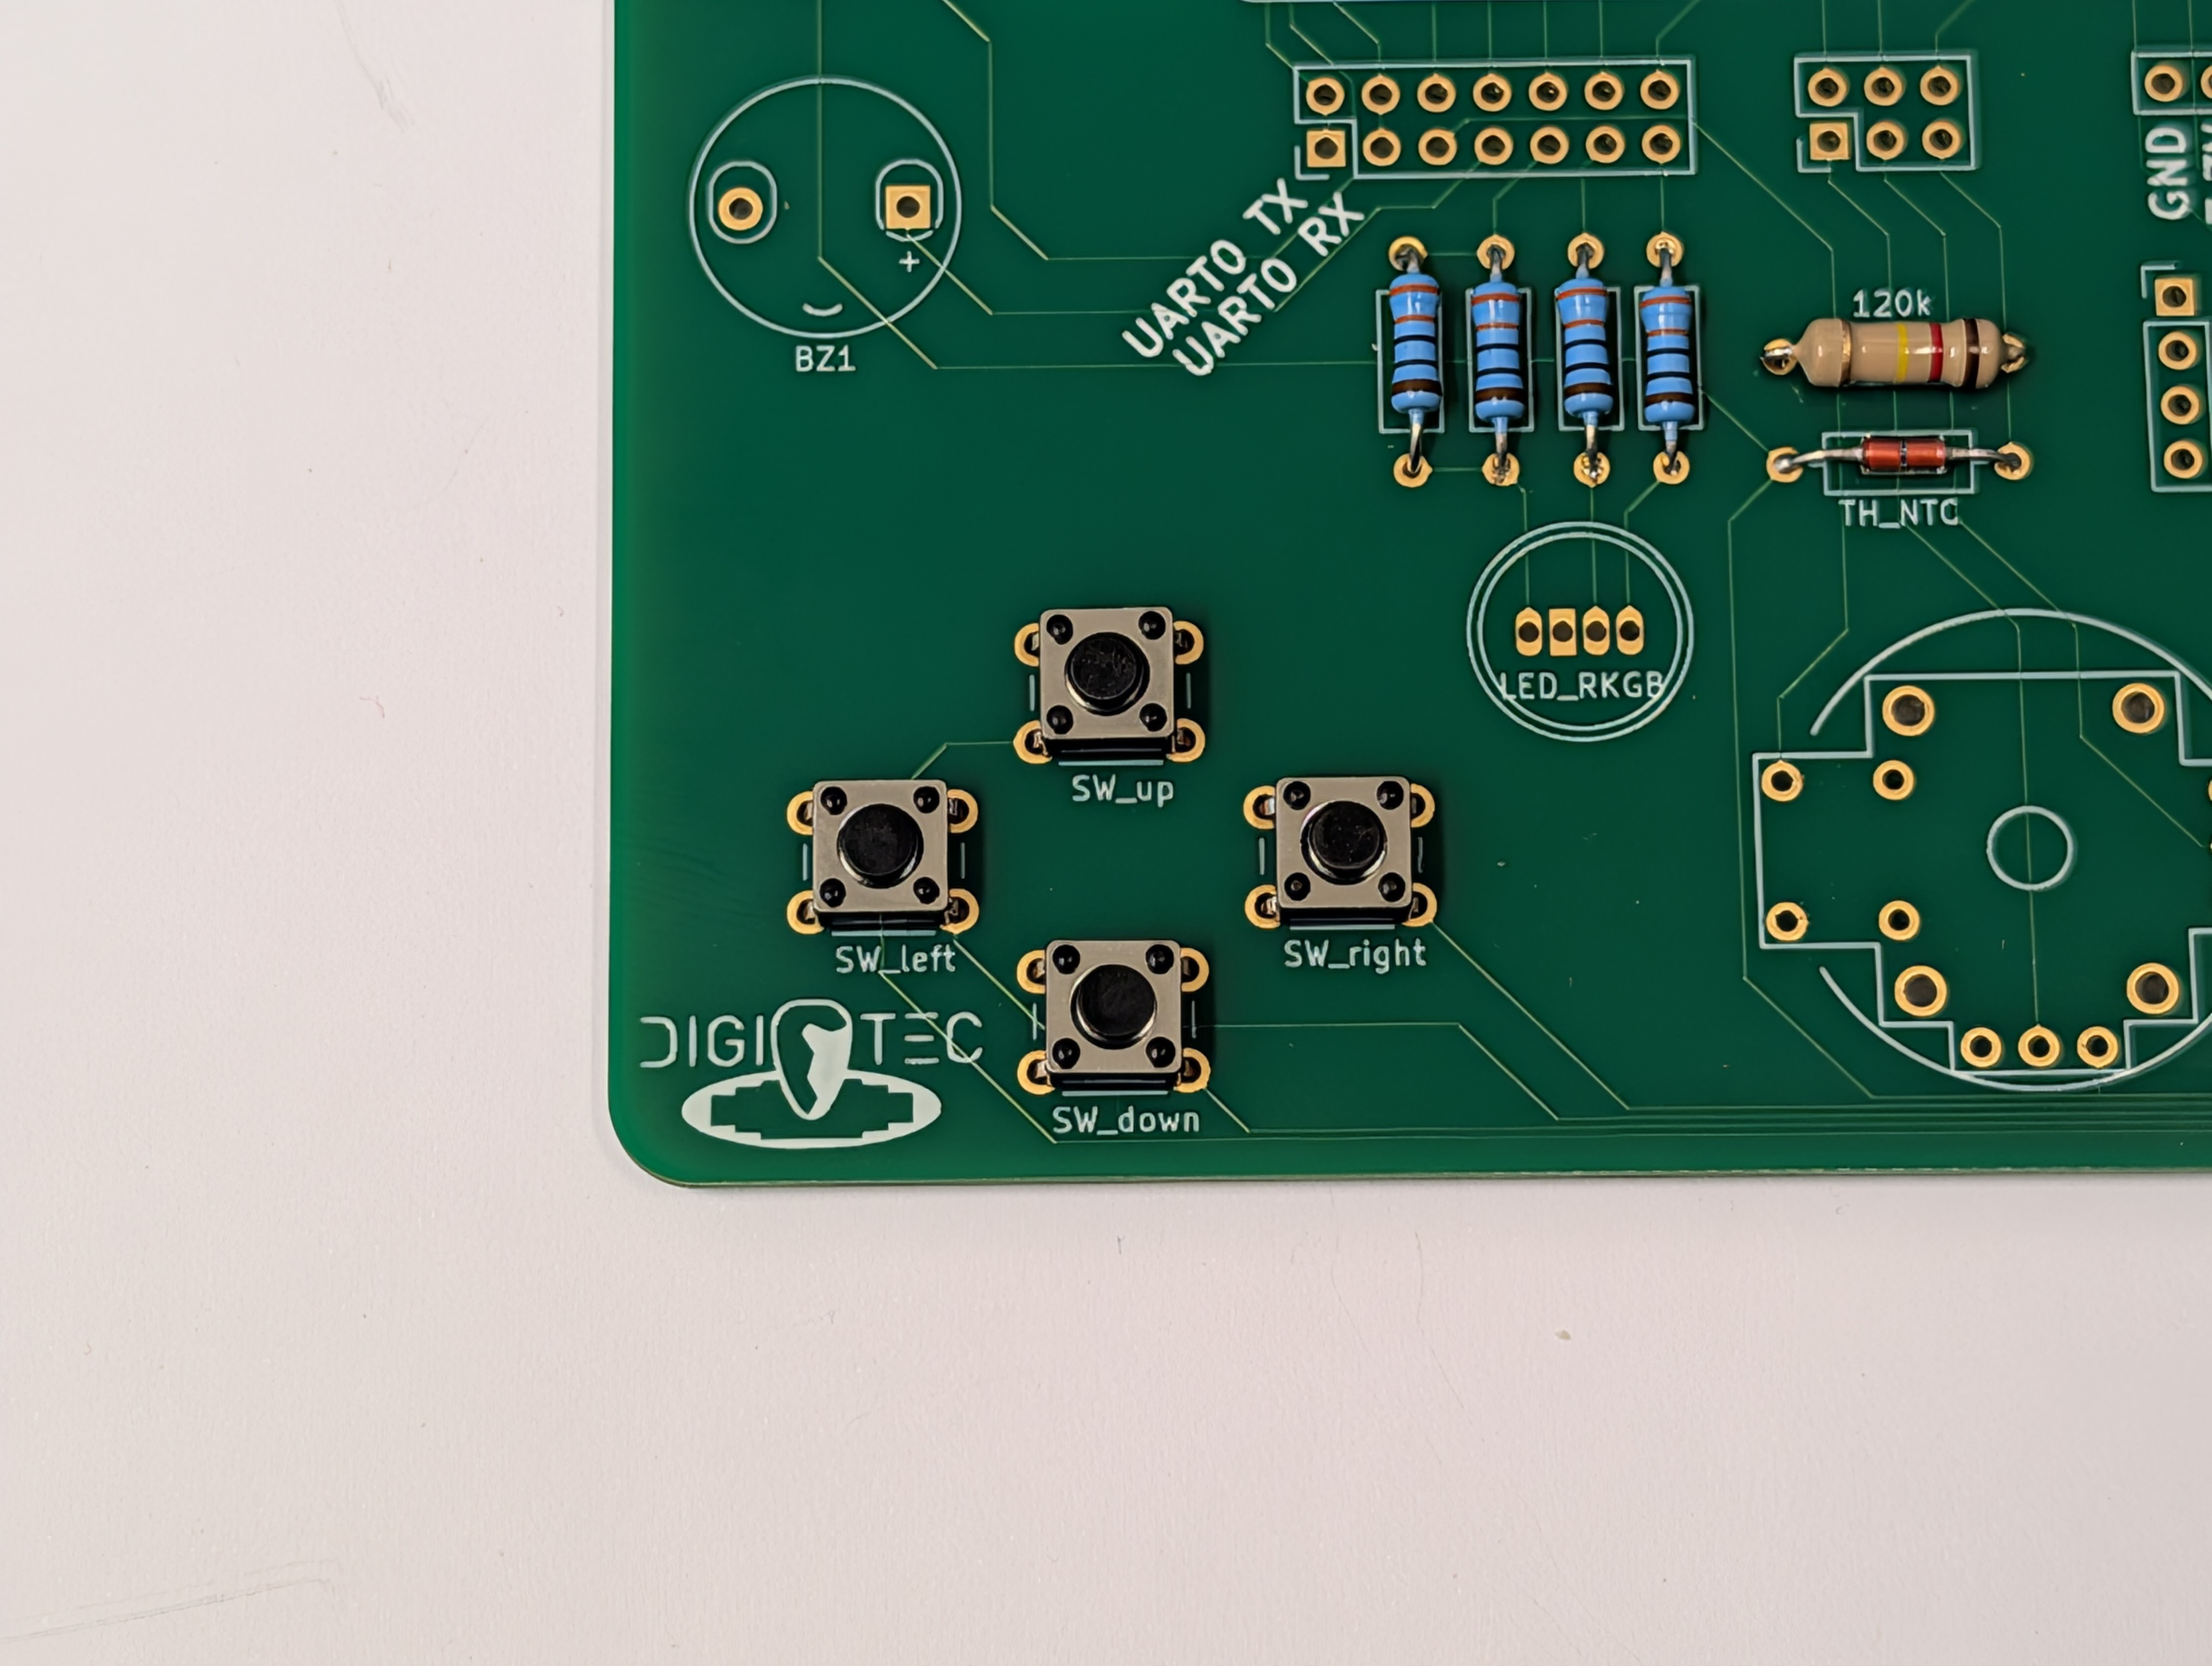
\includegraphics[width=0.75\textwidth]{pictures_of_construction/instruction_step_43.jpg}
\end{figure}

\subsection*{7. Stiftleisten auf die Hauptplatine löten}

Jetzt kommen mehrere Stiftleisten direkt auf die Buzzerino-Platine.

\textbf{Wichtig:}
\textbf{Die kurze Seite der Pins muss durch die Platine gesteckt werden.}

Das ist sehr wichtig und wird oft falsch gemacht.

Löte nacheinander:
\begin{itemize}
    \item die 2x7-Stiftleiste
    \item die 2x3-Stiftleiste
    \item die 2x16-Stiftleiste
    \item die 1x3-Stiftleiste
\end{itemize}

So gehst du immer vor:
\begin{enumerate}
    \item Stiftleiste einsetzen
    \item einen Pin löten
    \item prüfen, ob sie gerade sitzt
    \item falls nötig korrigieren
    \item alle restlichen Pins löten
\end{enumerate}

\begin{figure}[H]
    \centering
    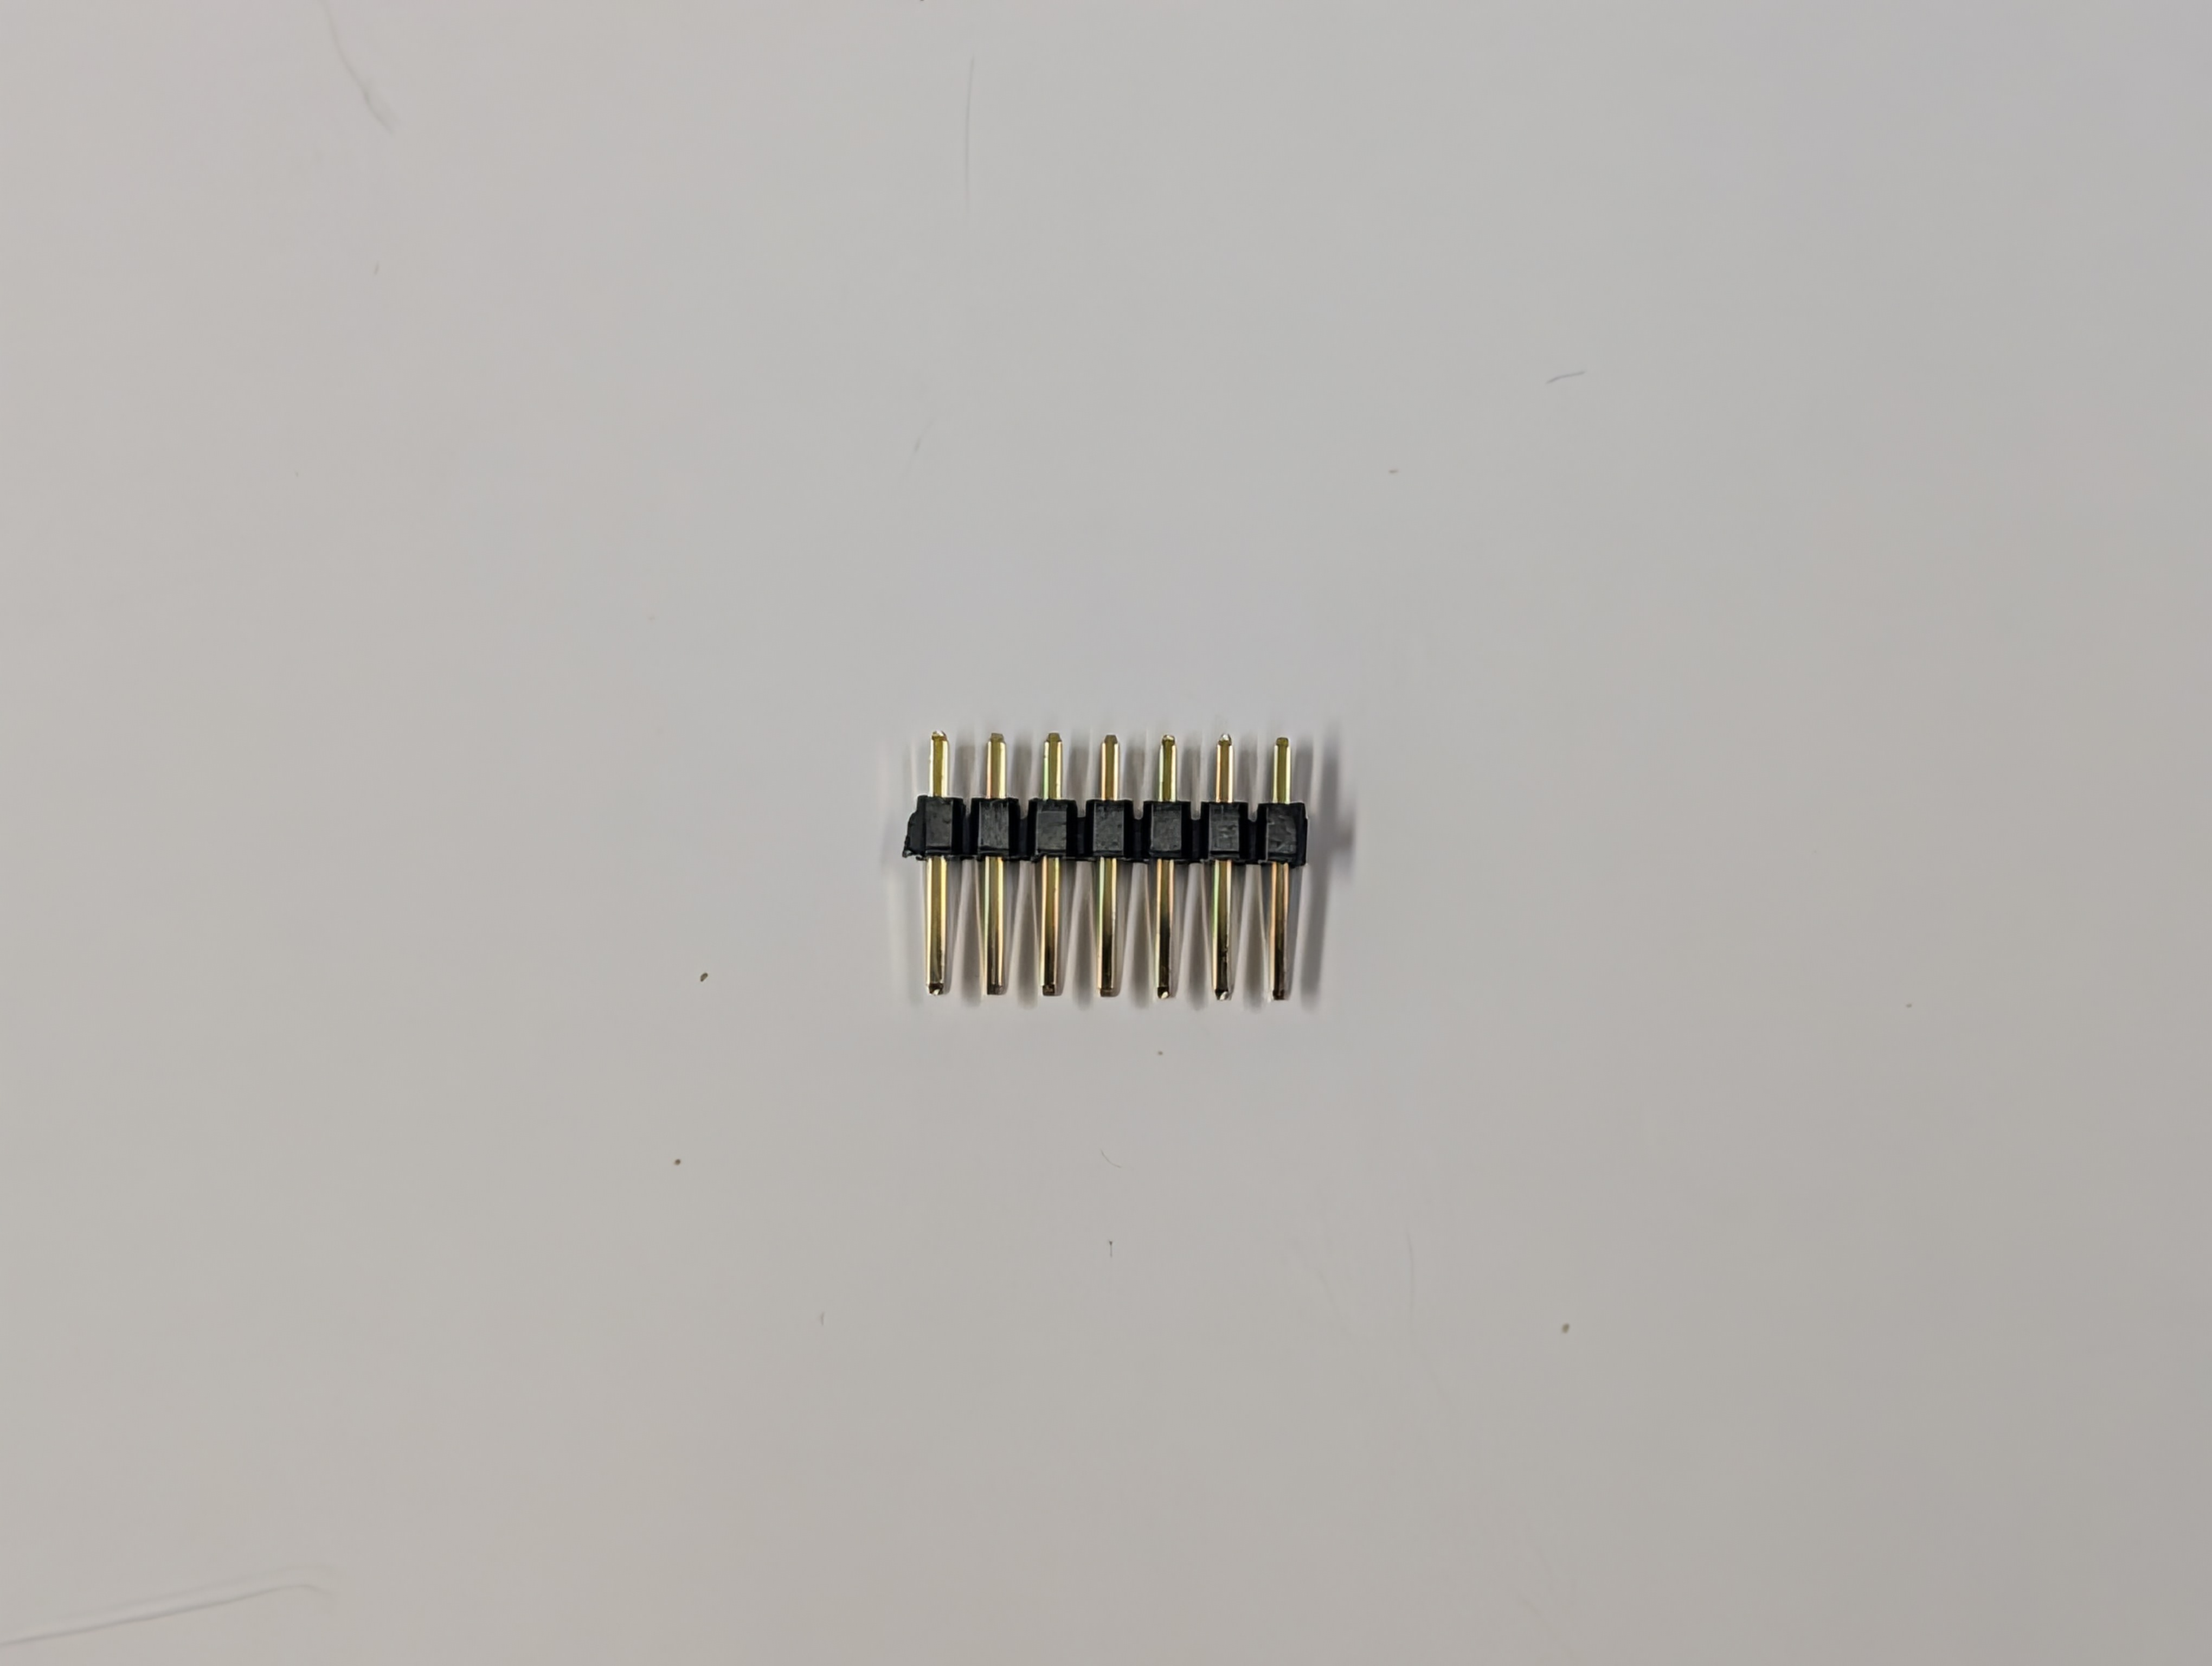
\includegraphics[width=0.75\textwidth]{pictures_of_construction/instruction_step_44.jpg}
\end{figure}

\begin{figure}[H]
    \centering
    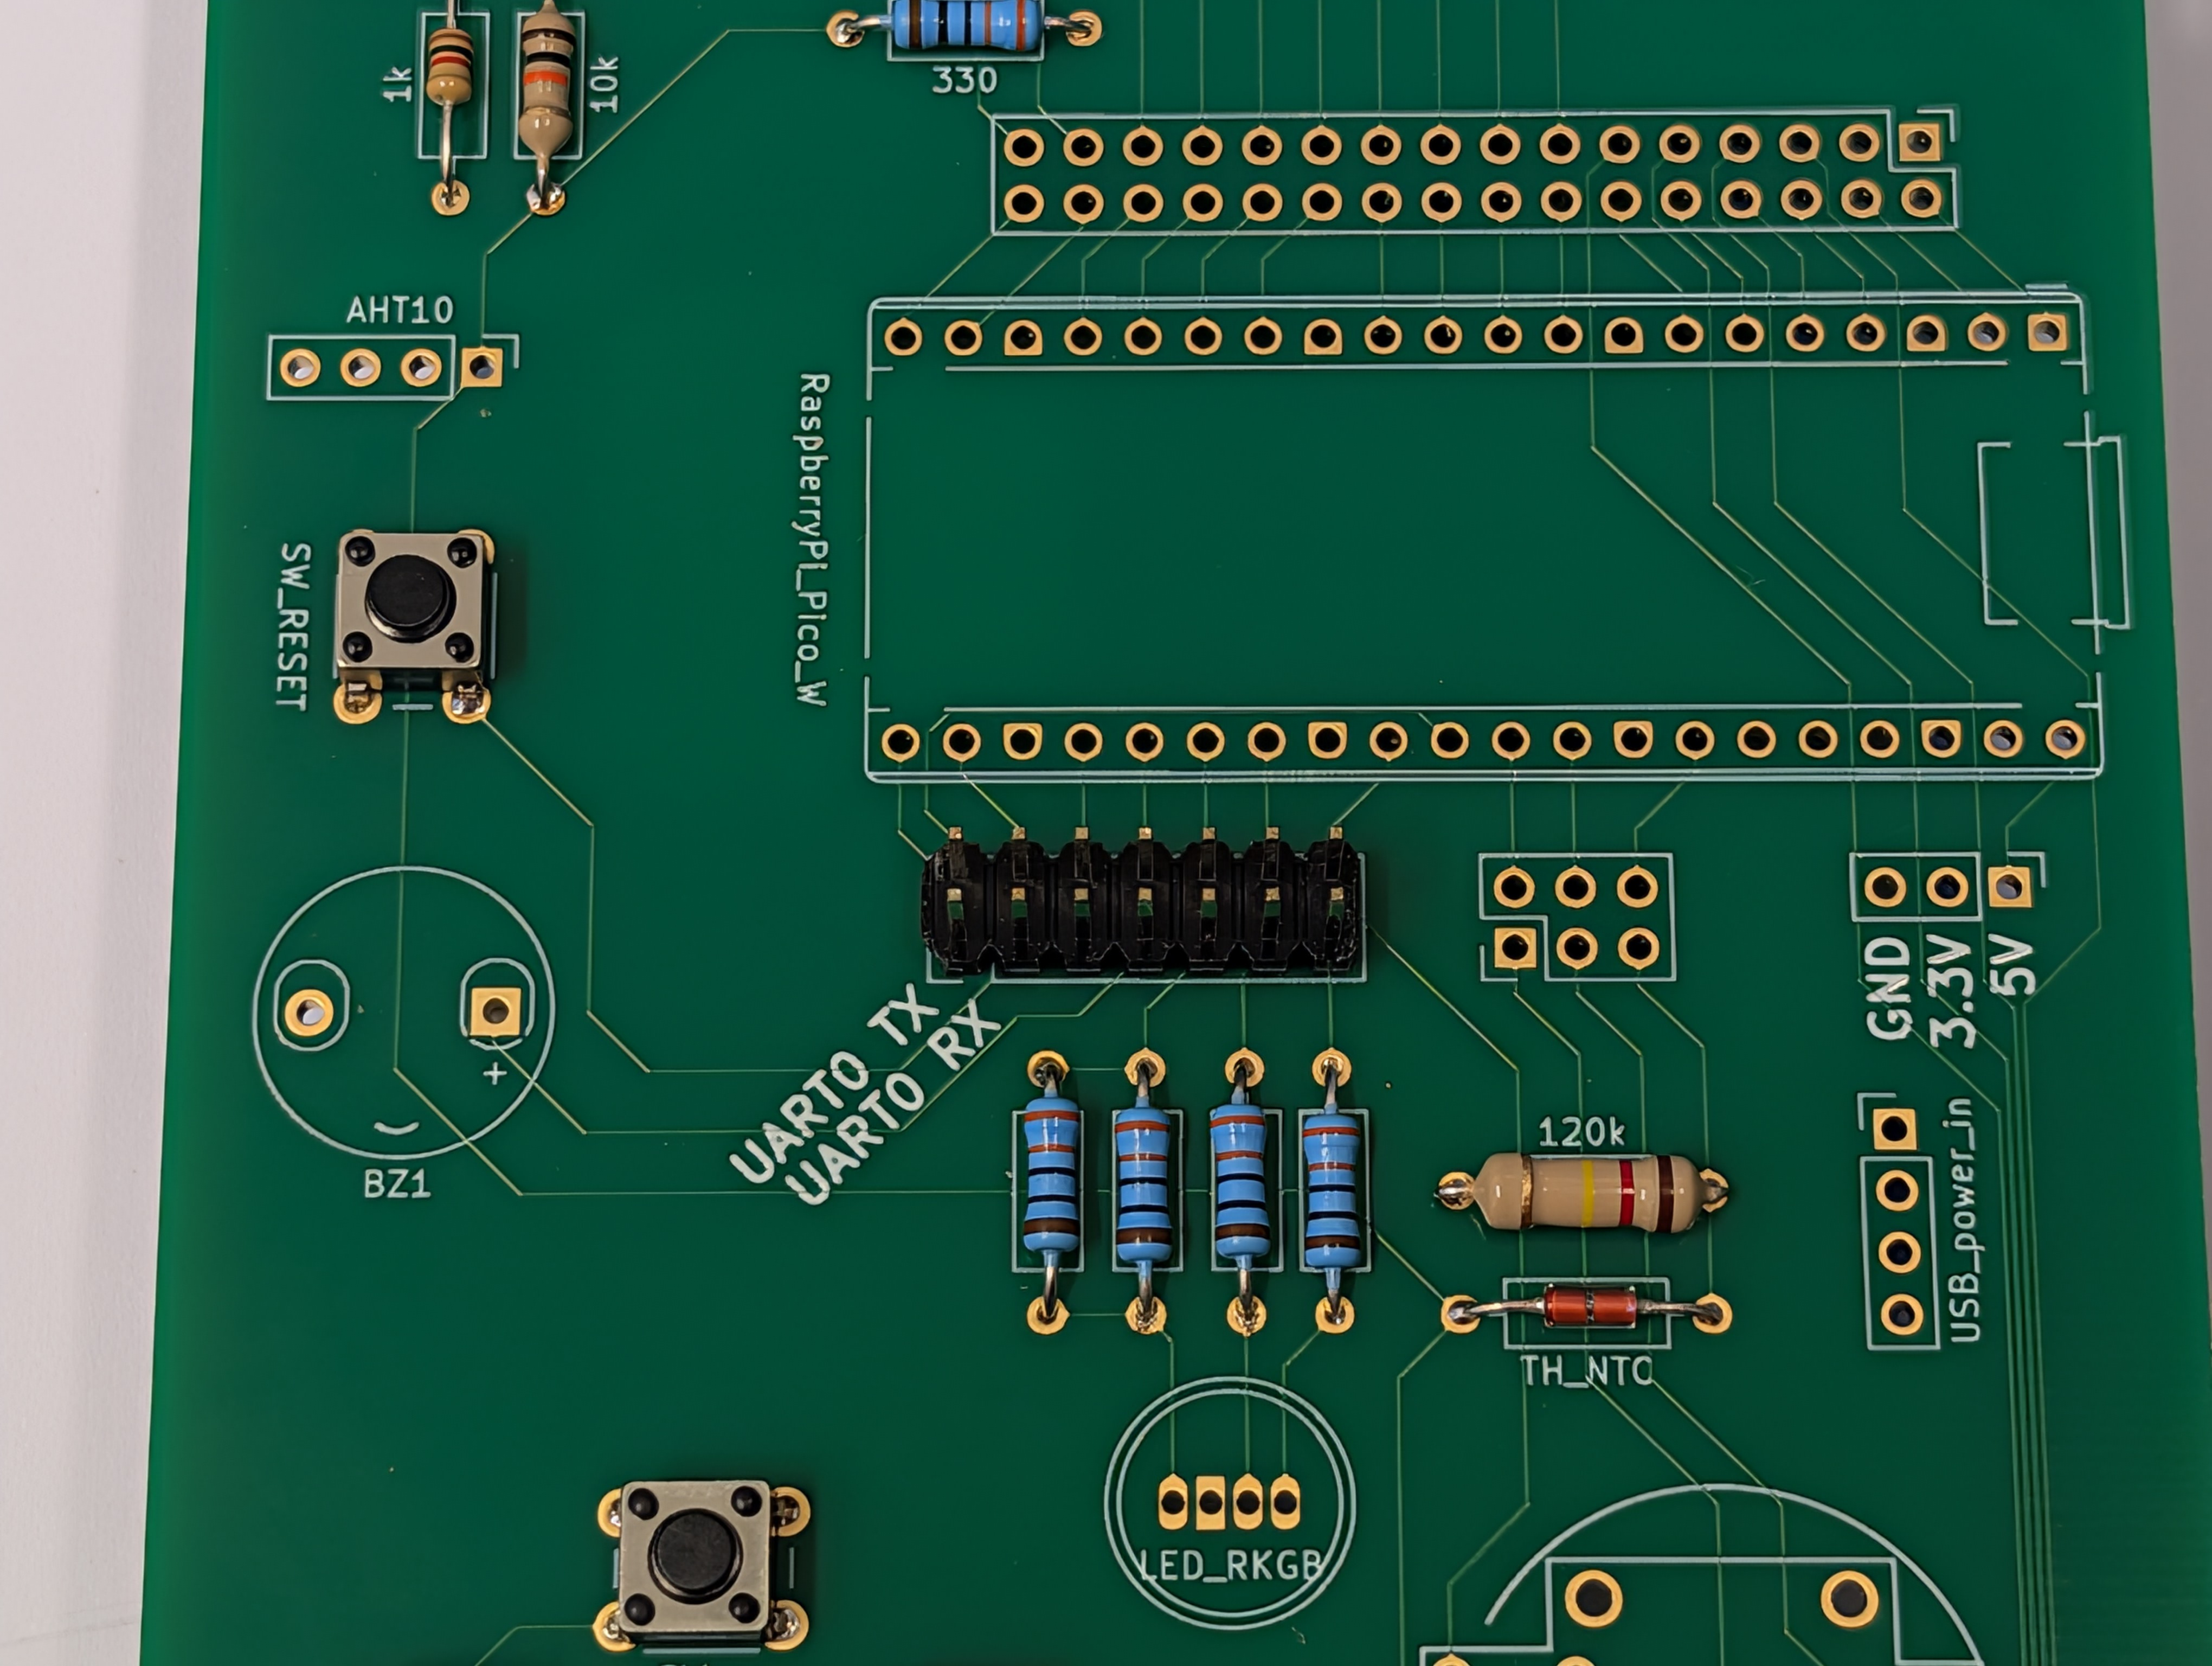
\includegraphics[width=0.75\textwidth]{pictures_of_construction/instruction_step_45.jpg}
\end{figure}

\begin{figure}[H]
    \centering
    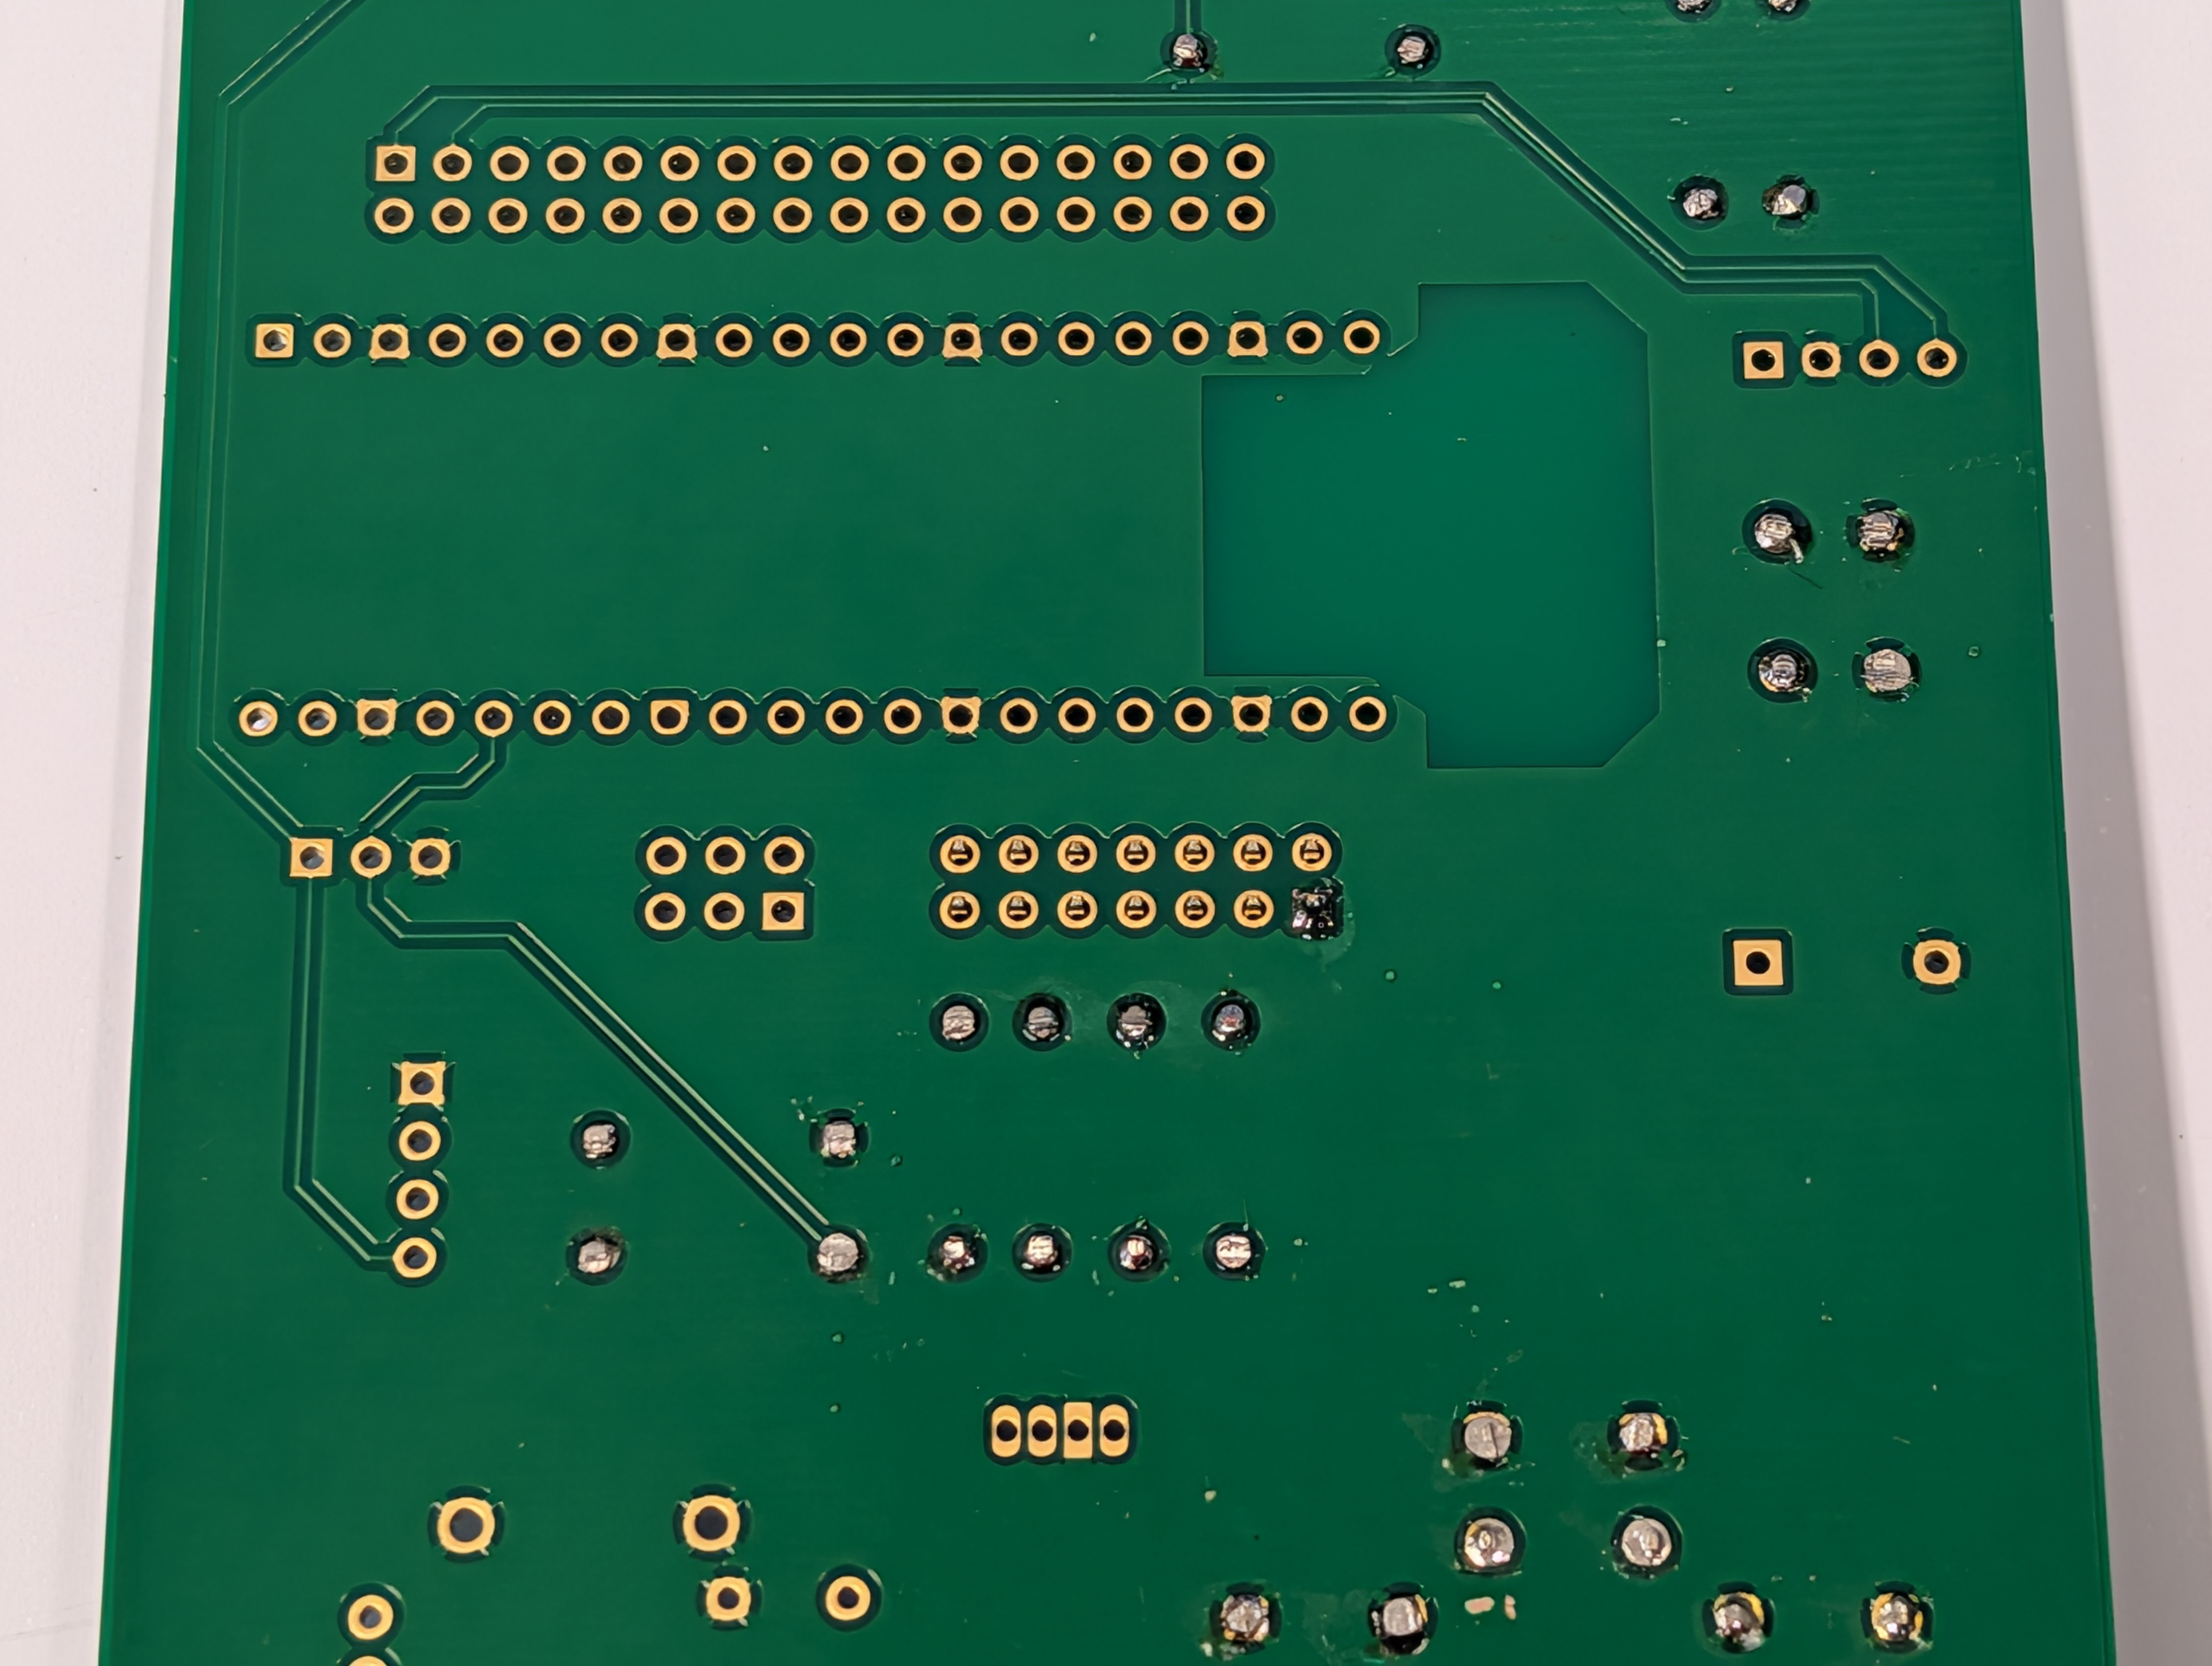
\includegraphics[width=0.75\textwidth]{pictures_of_construction/instruction_step_46.jpg}
\end{figure}

\begin{figure}[H]
    \centering
    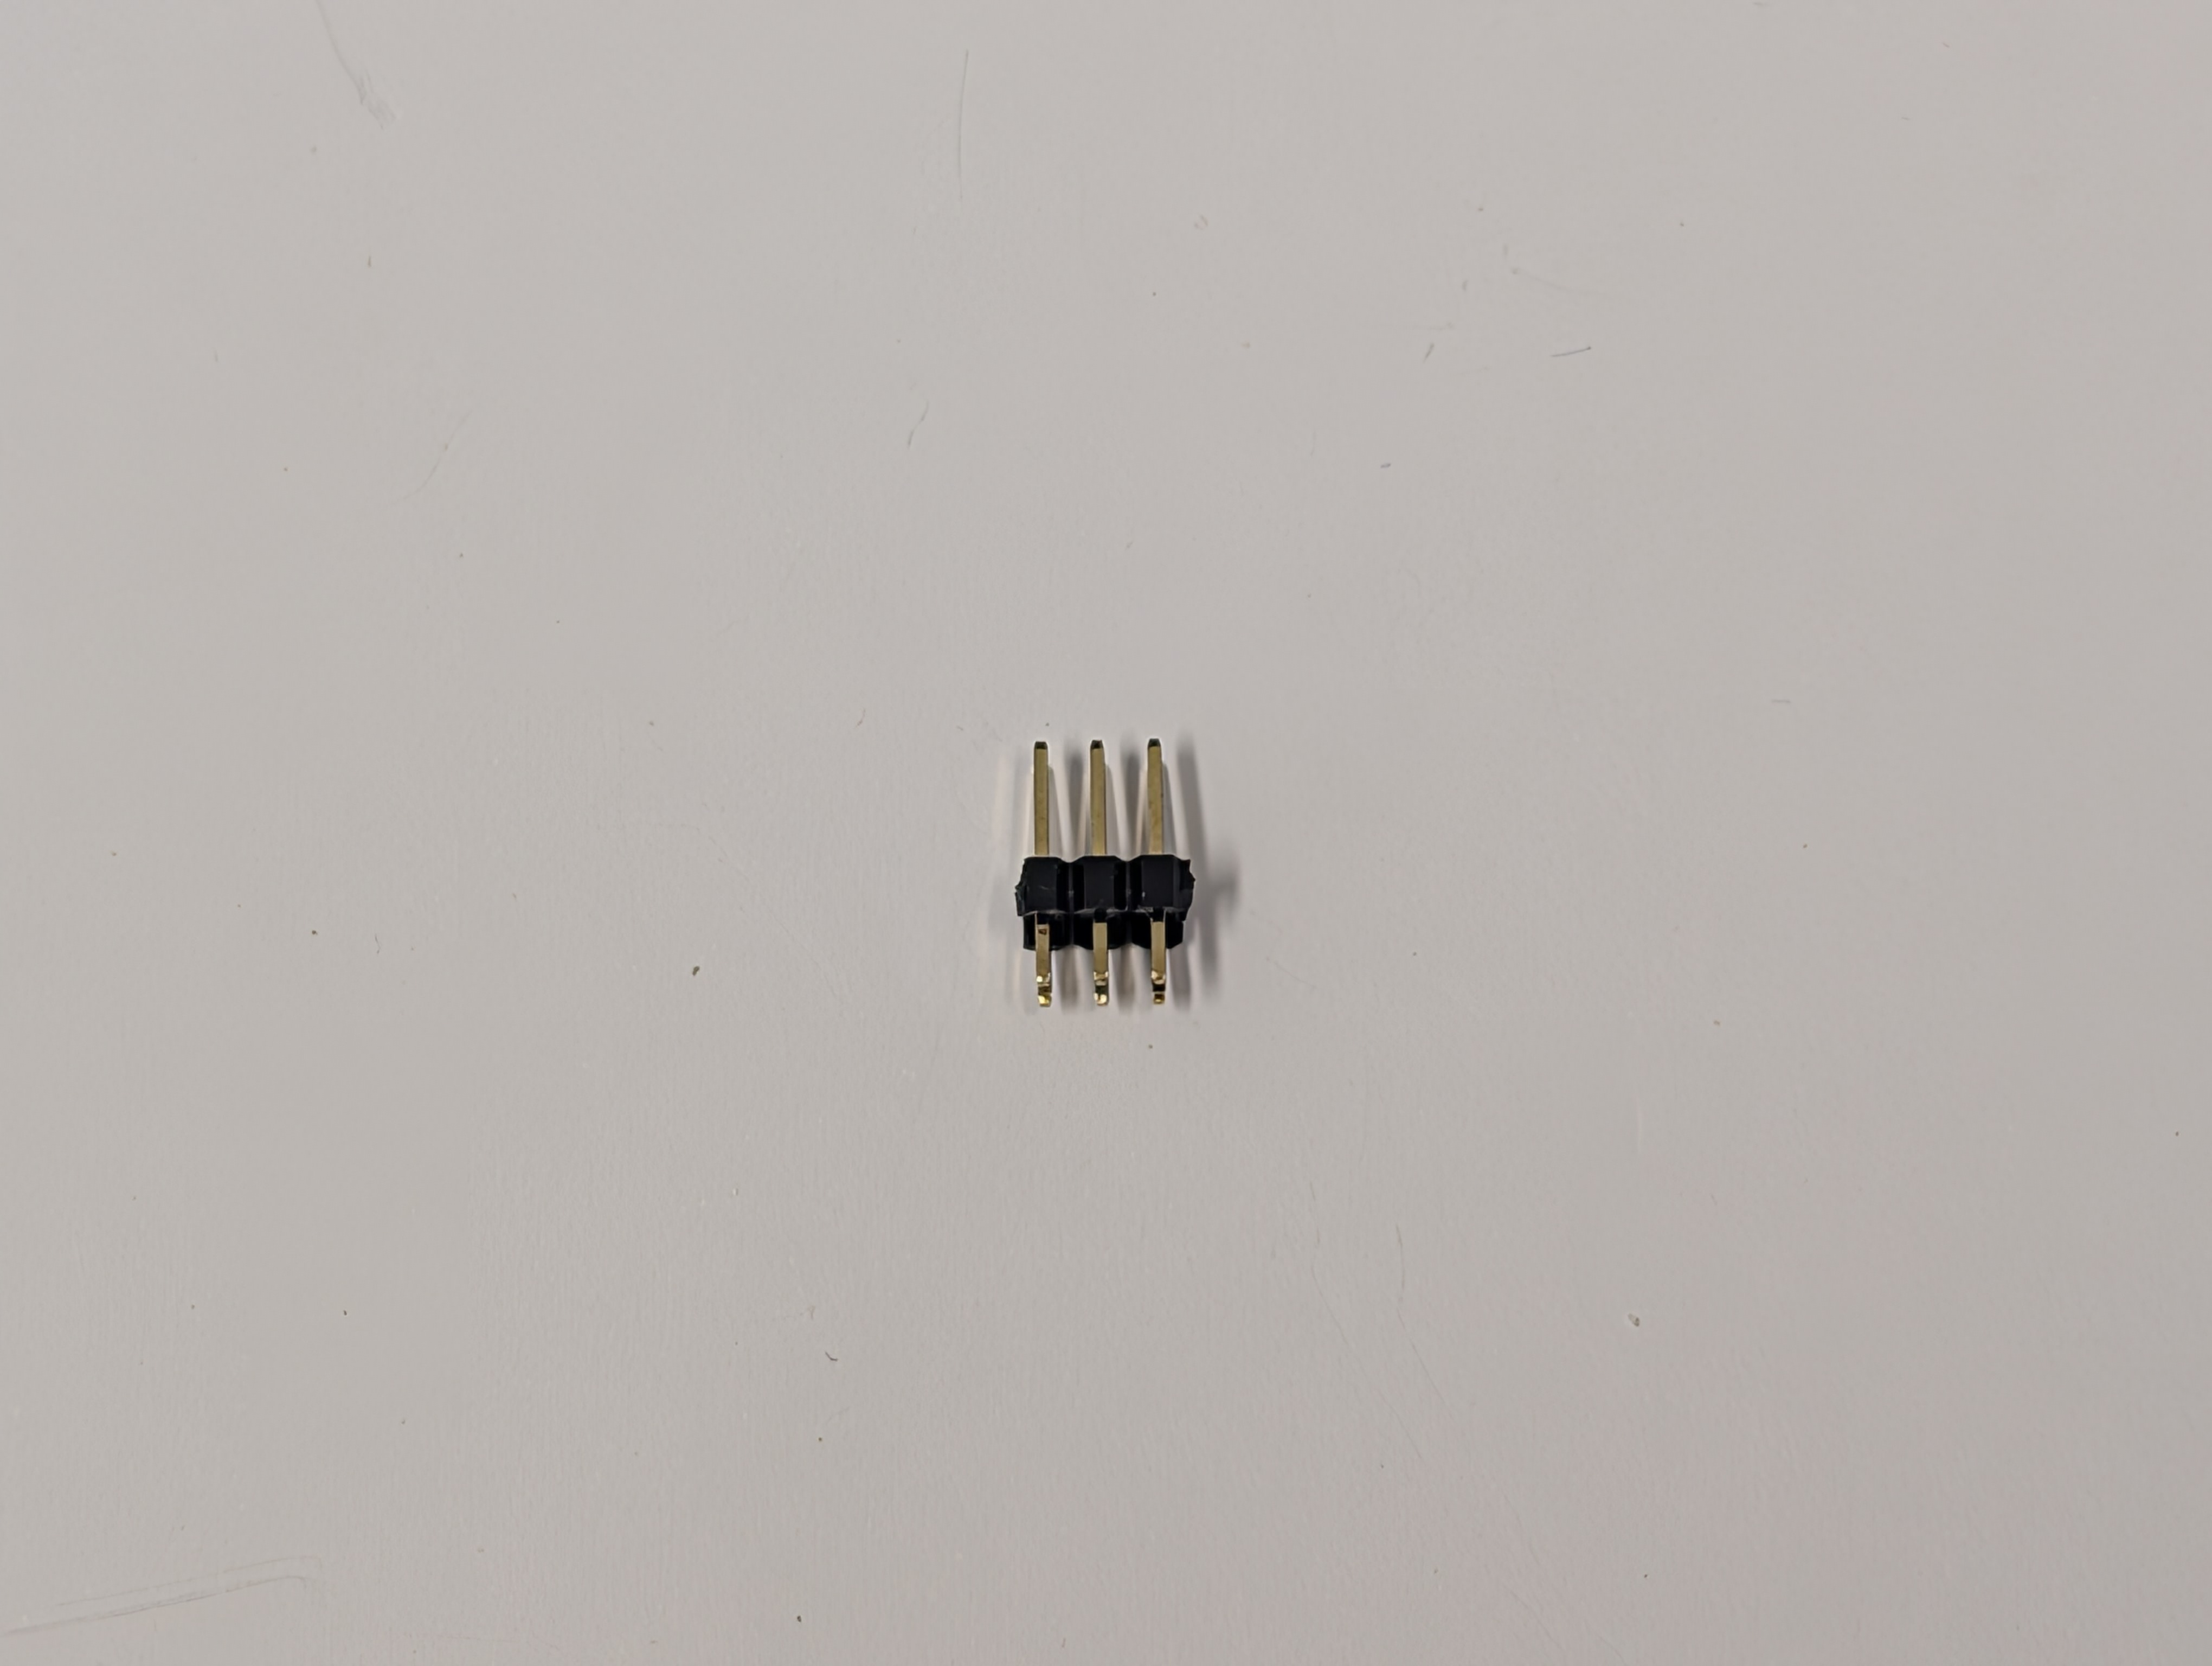
\includegraphics[width=0.75\textwidth]{pictures_of_construction/instruction_step_47.jpg}
\end{figure}

\begin{figure}[H]
    \centering
    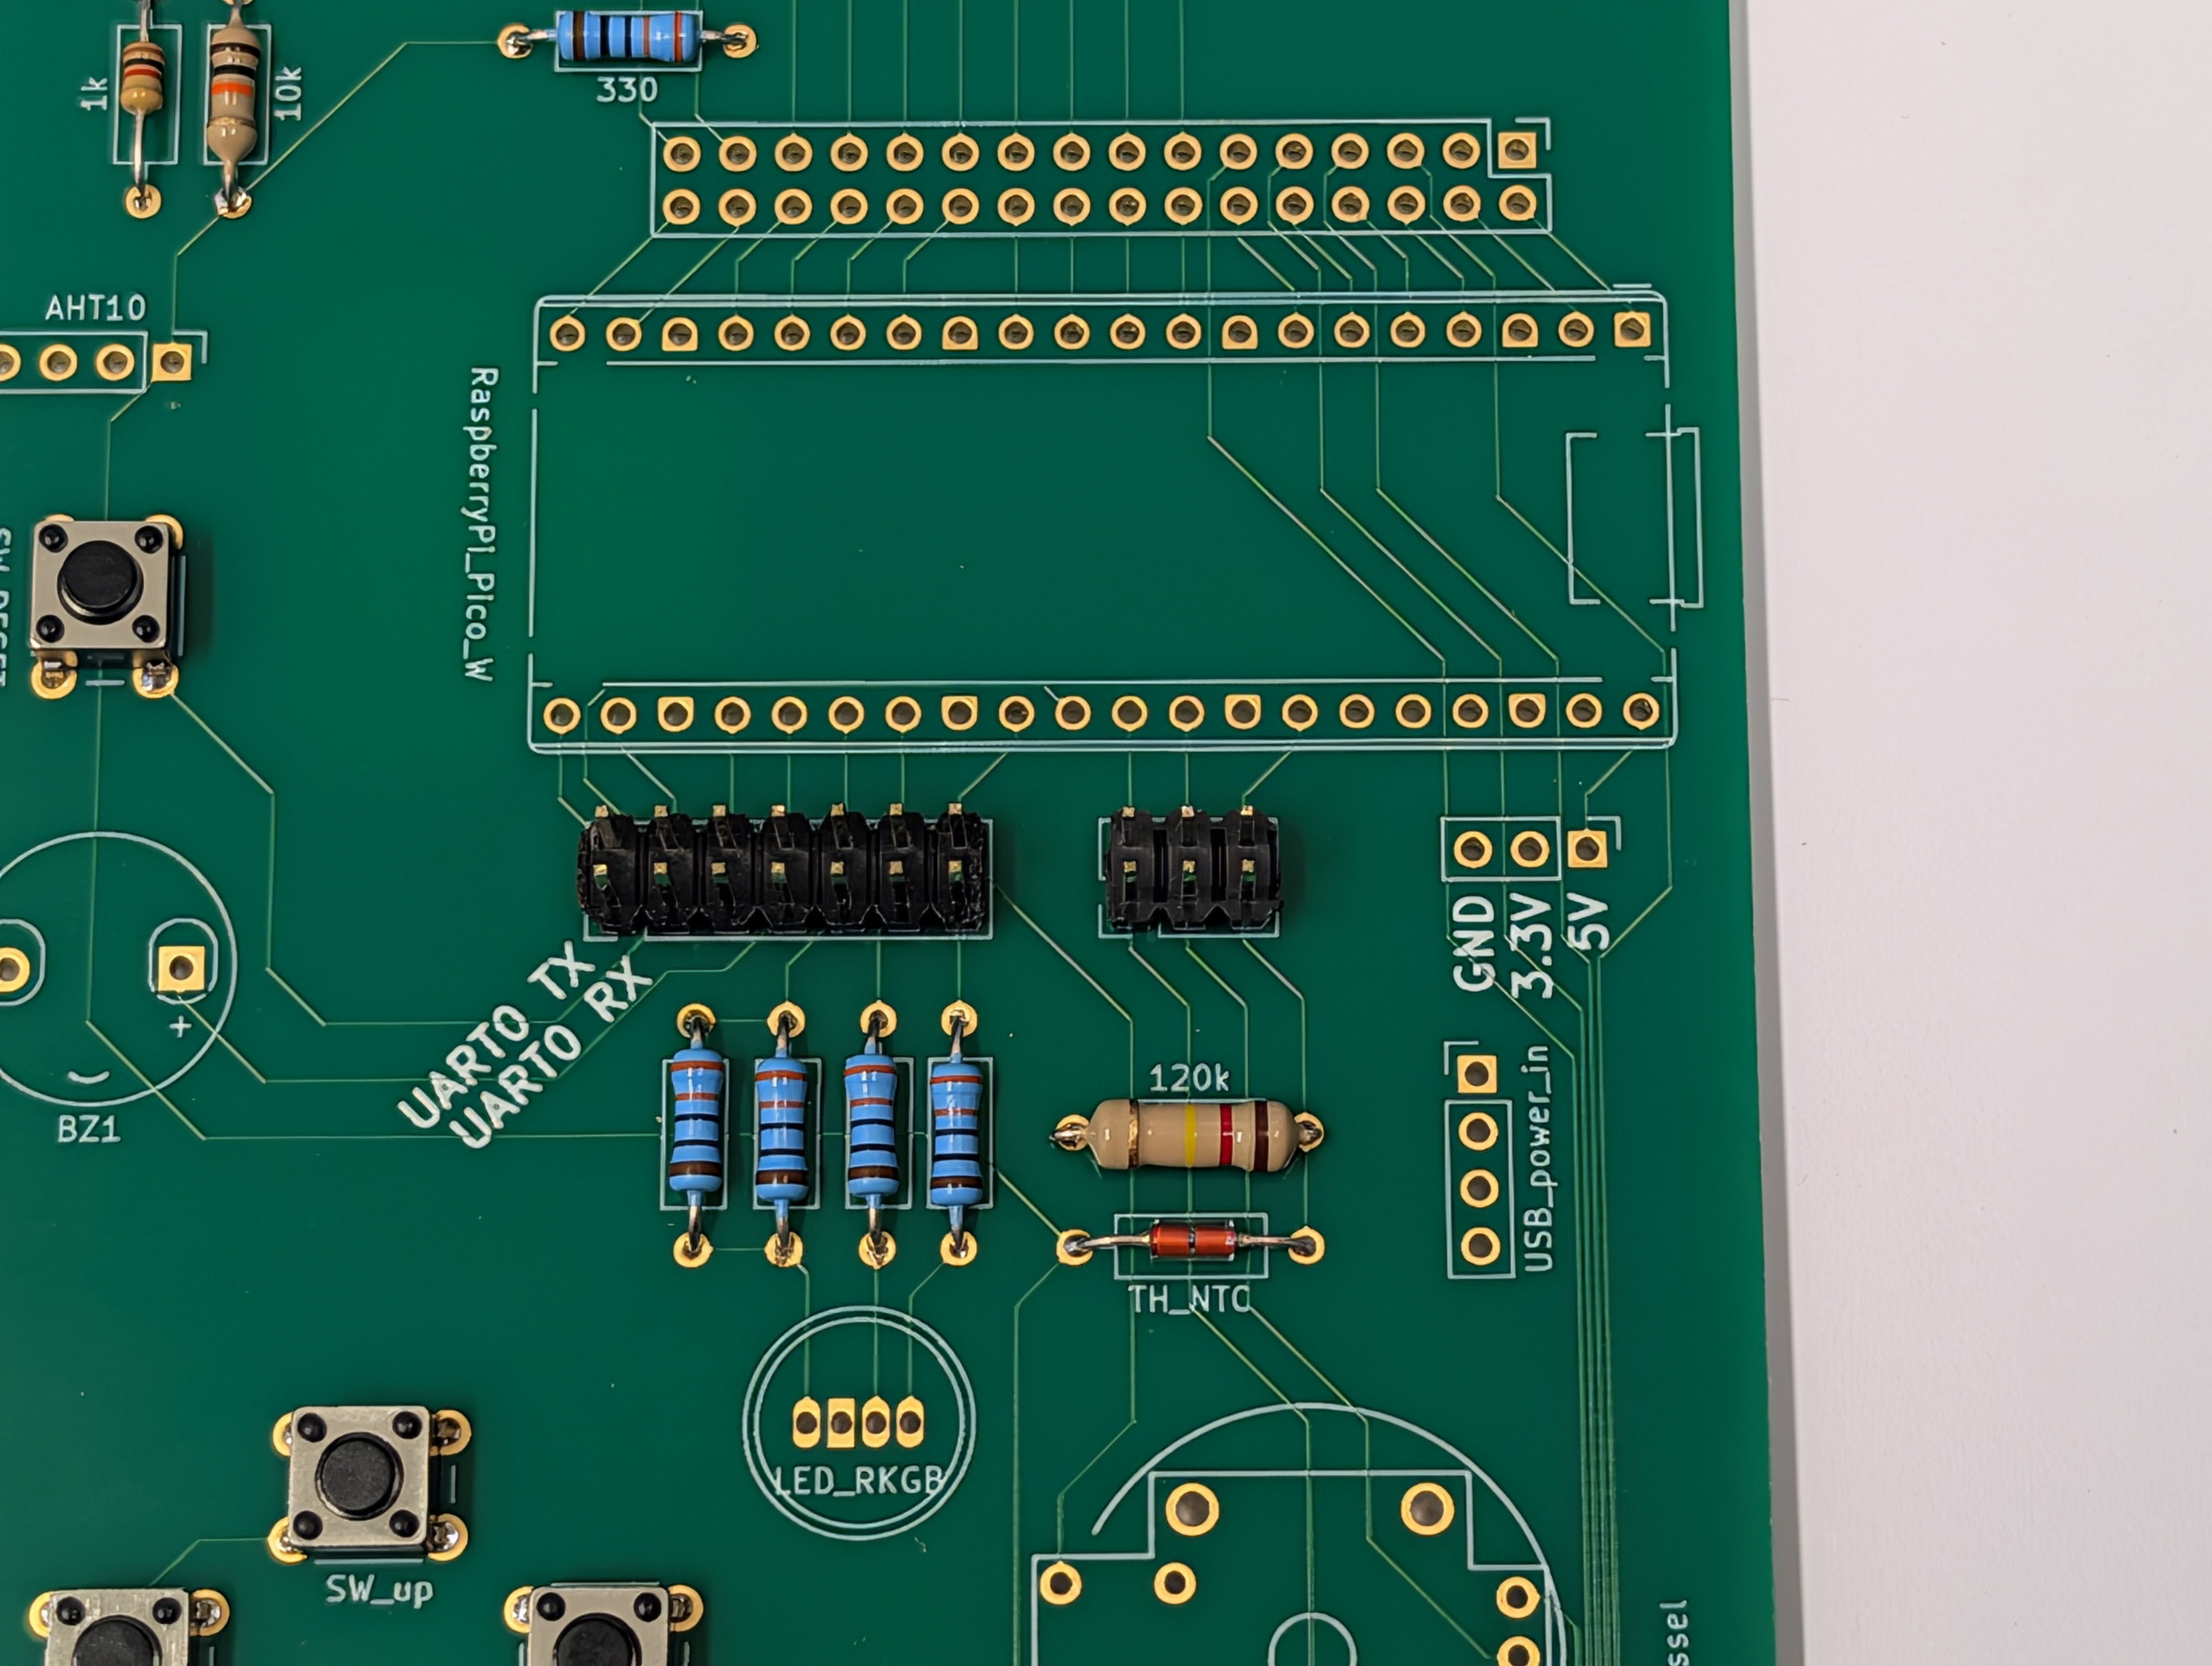
\includegraphics[width=0.75\textwidth]{pictures_of_construction/instruction_step_48.jpg}
\end{figure}

\begin{figure}[H]
    \centering
    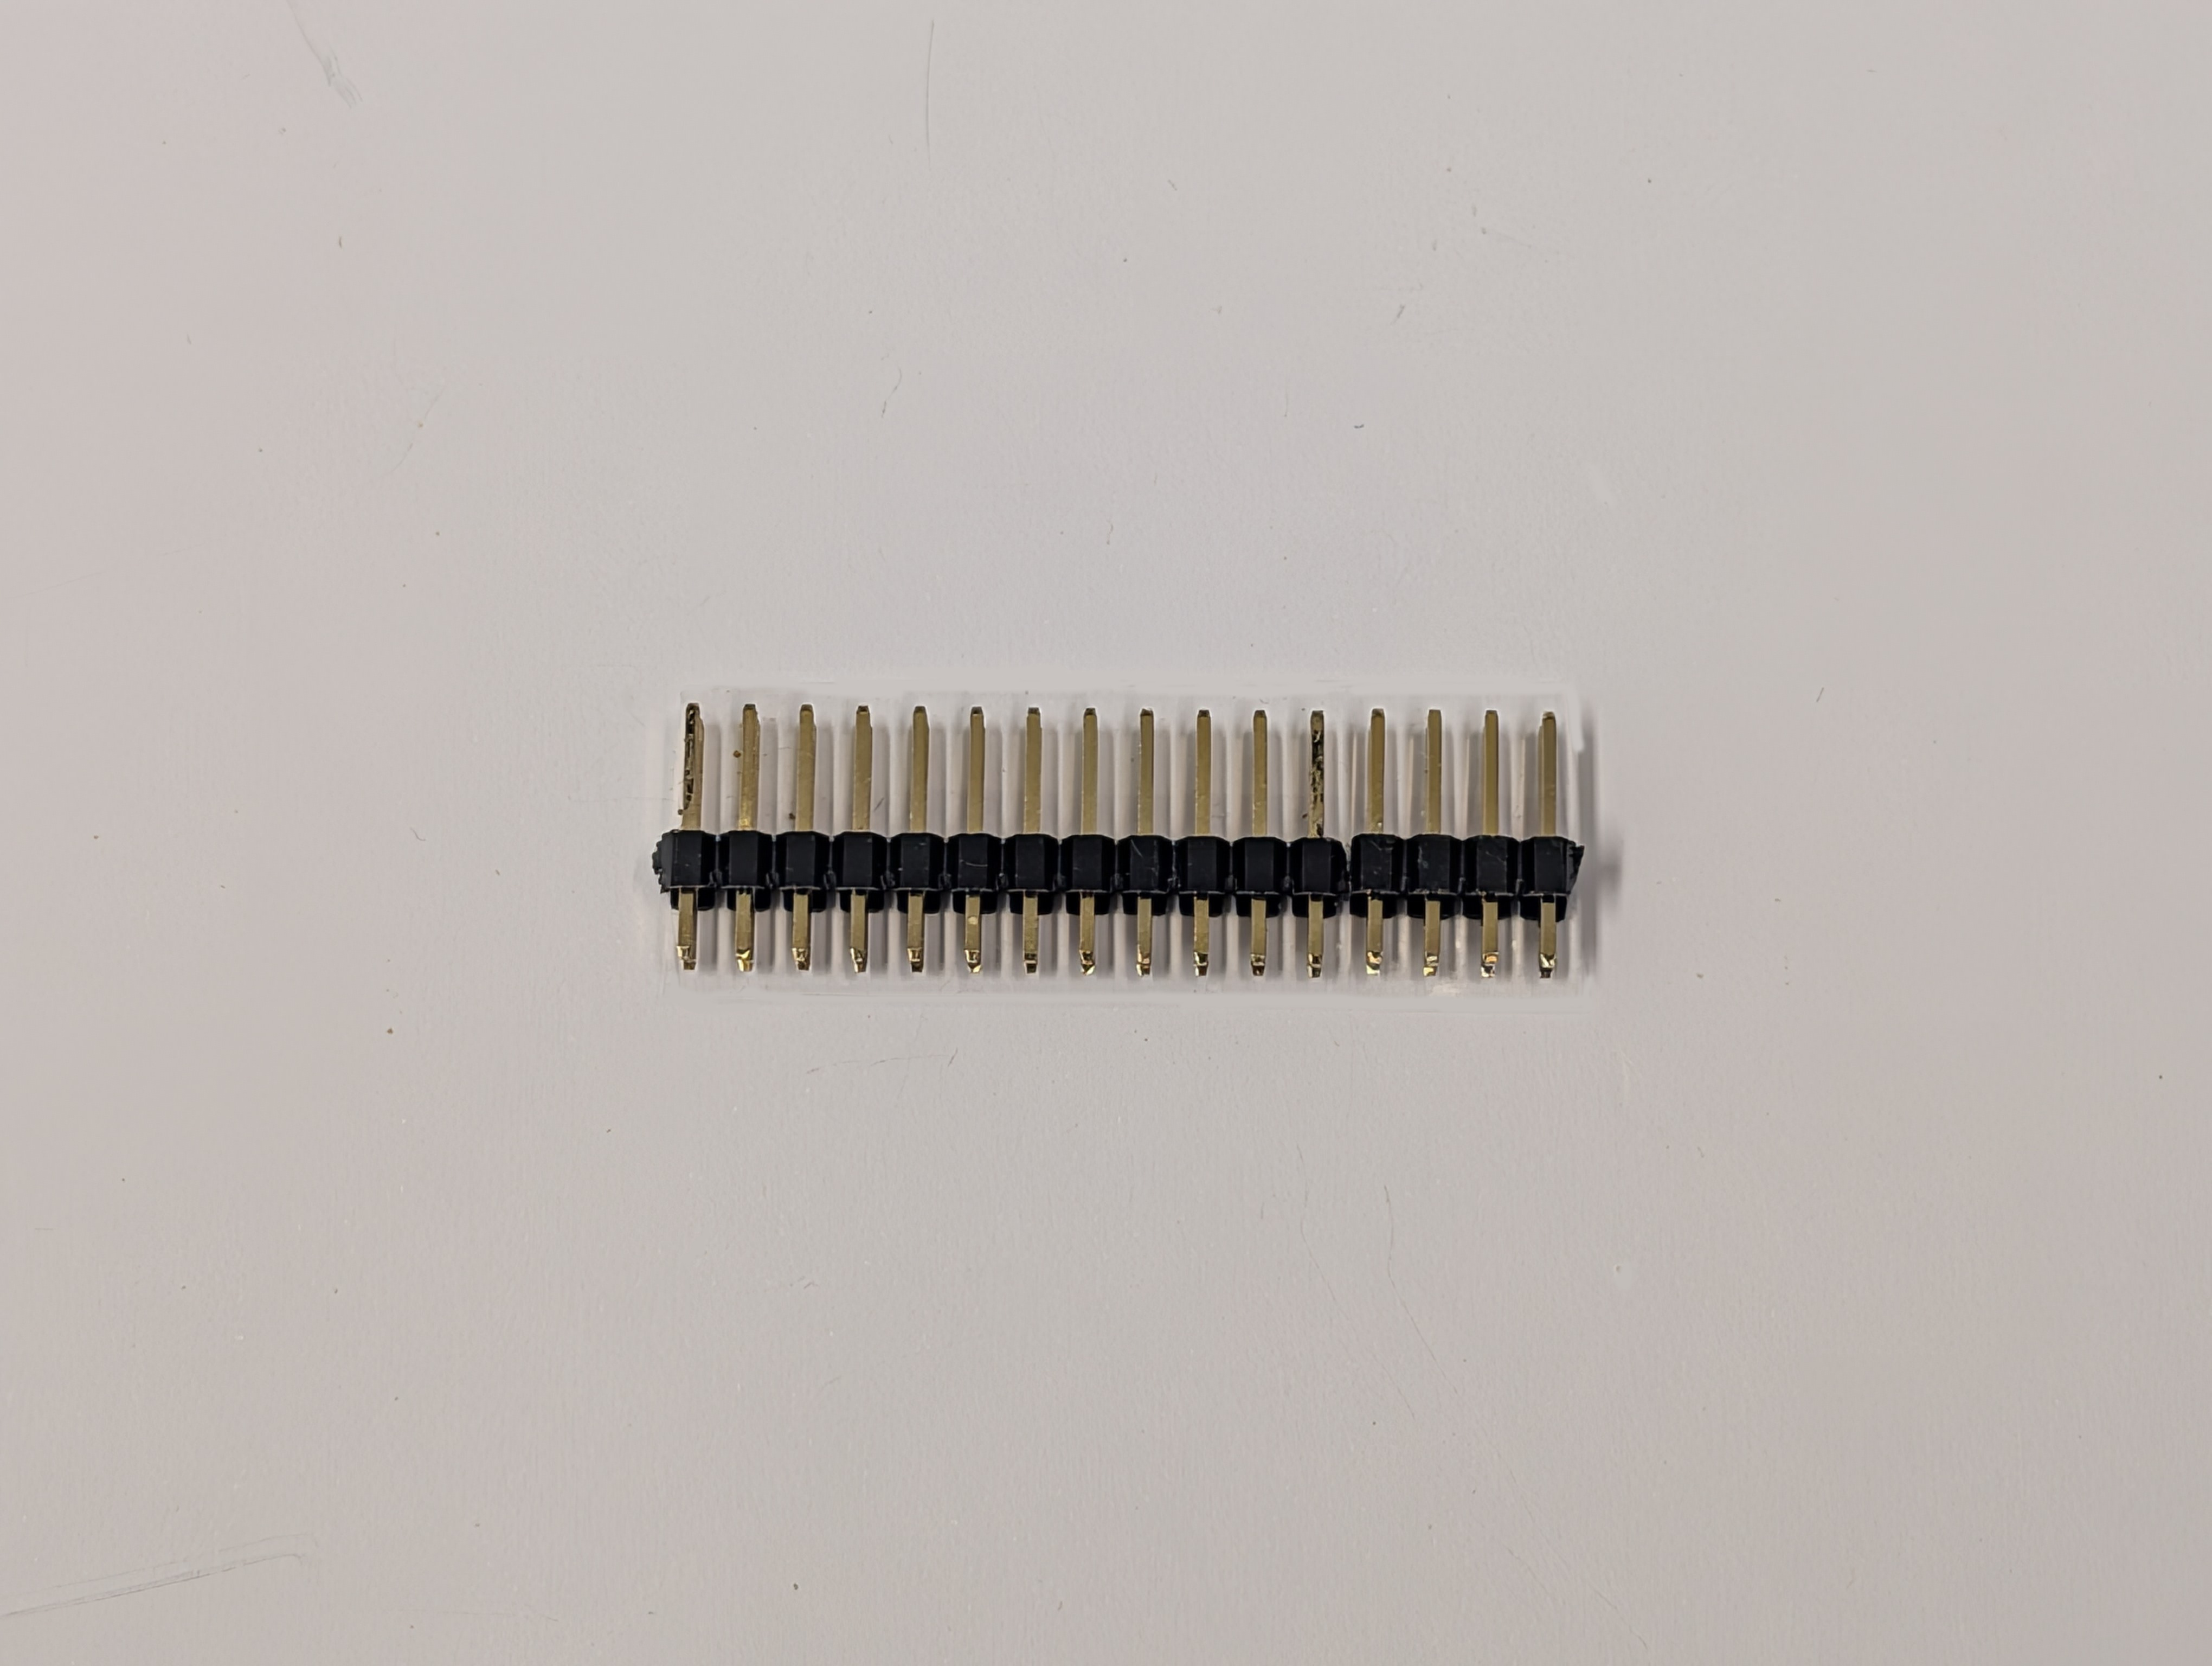
\includegraphics[width=0.75\textwidth]{pictures_of_construction/instruction_step_49.jpg}
\end{figure}

\begin{figure}[H]
    \centering
    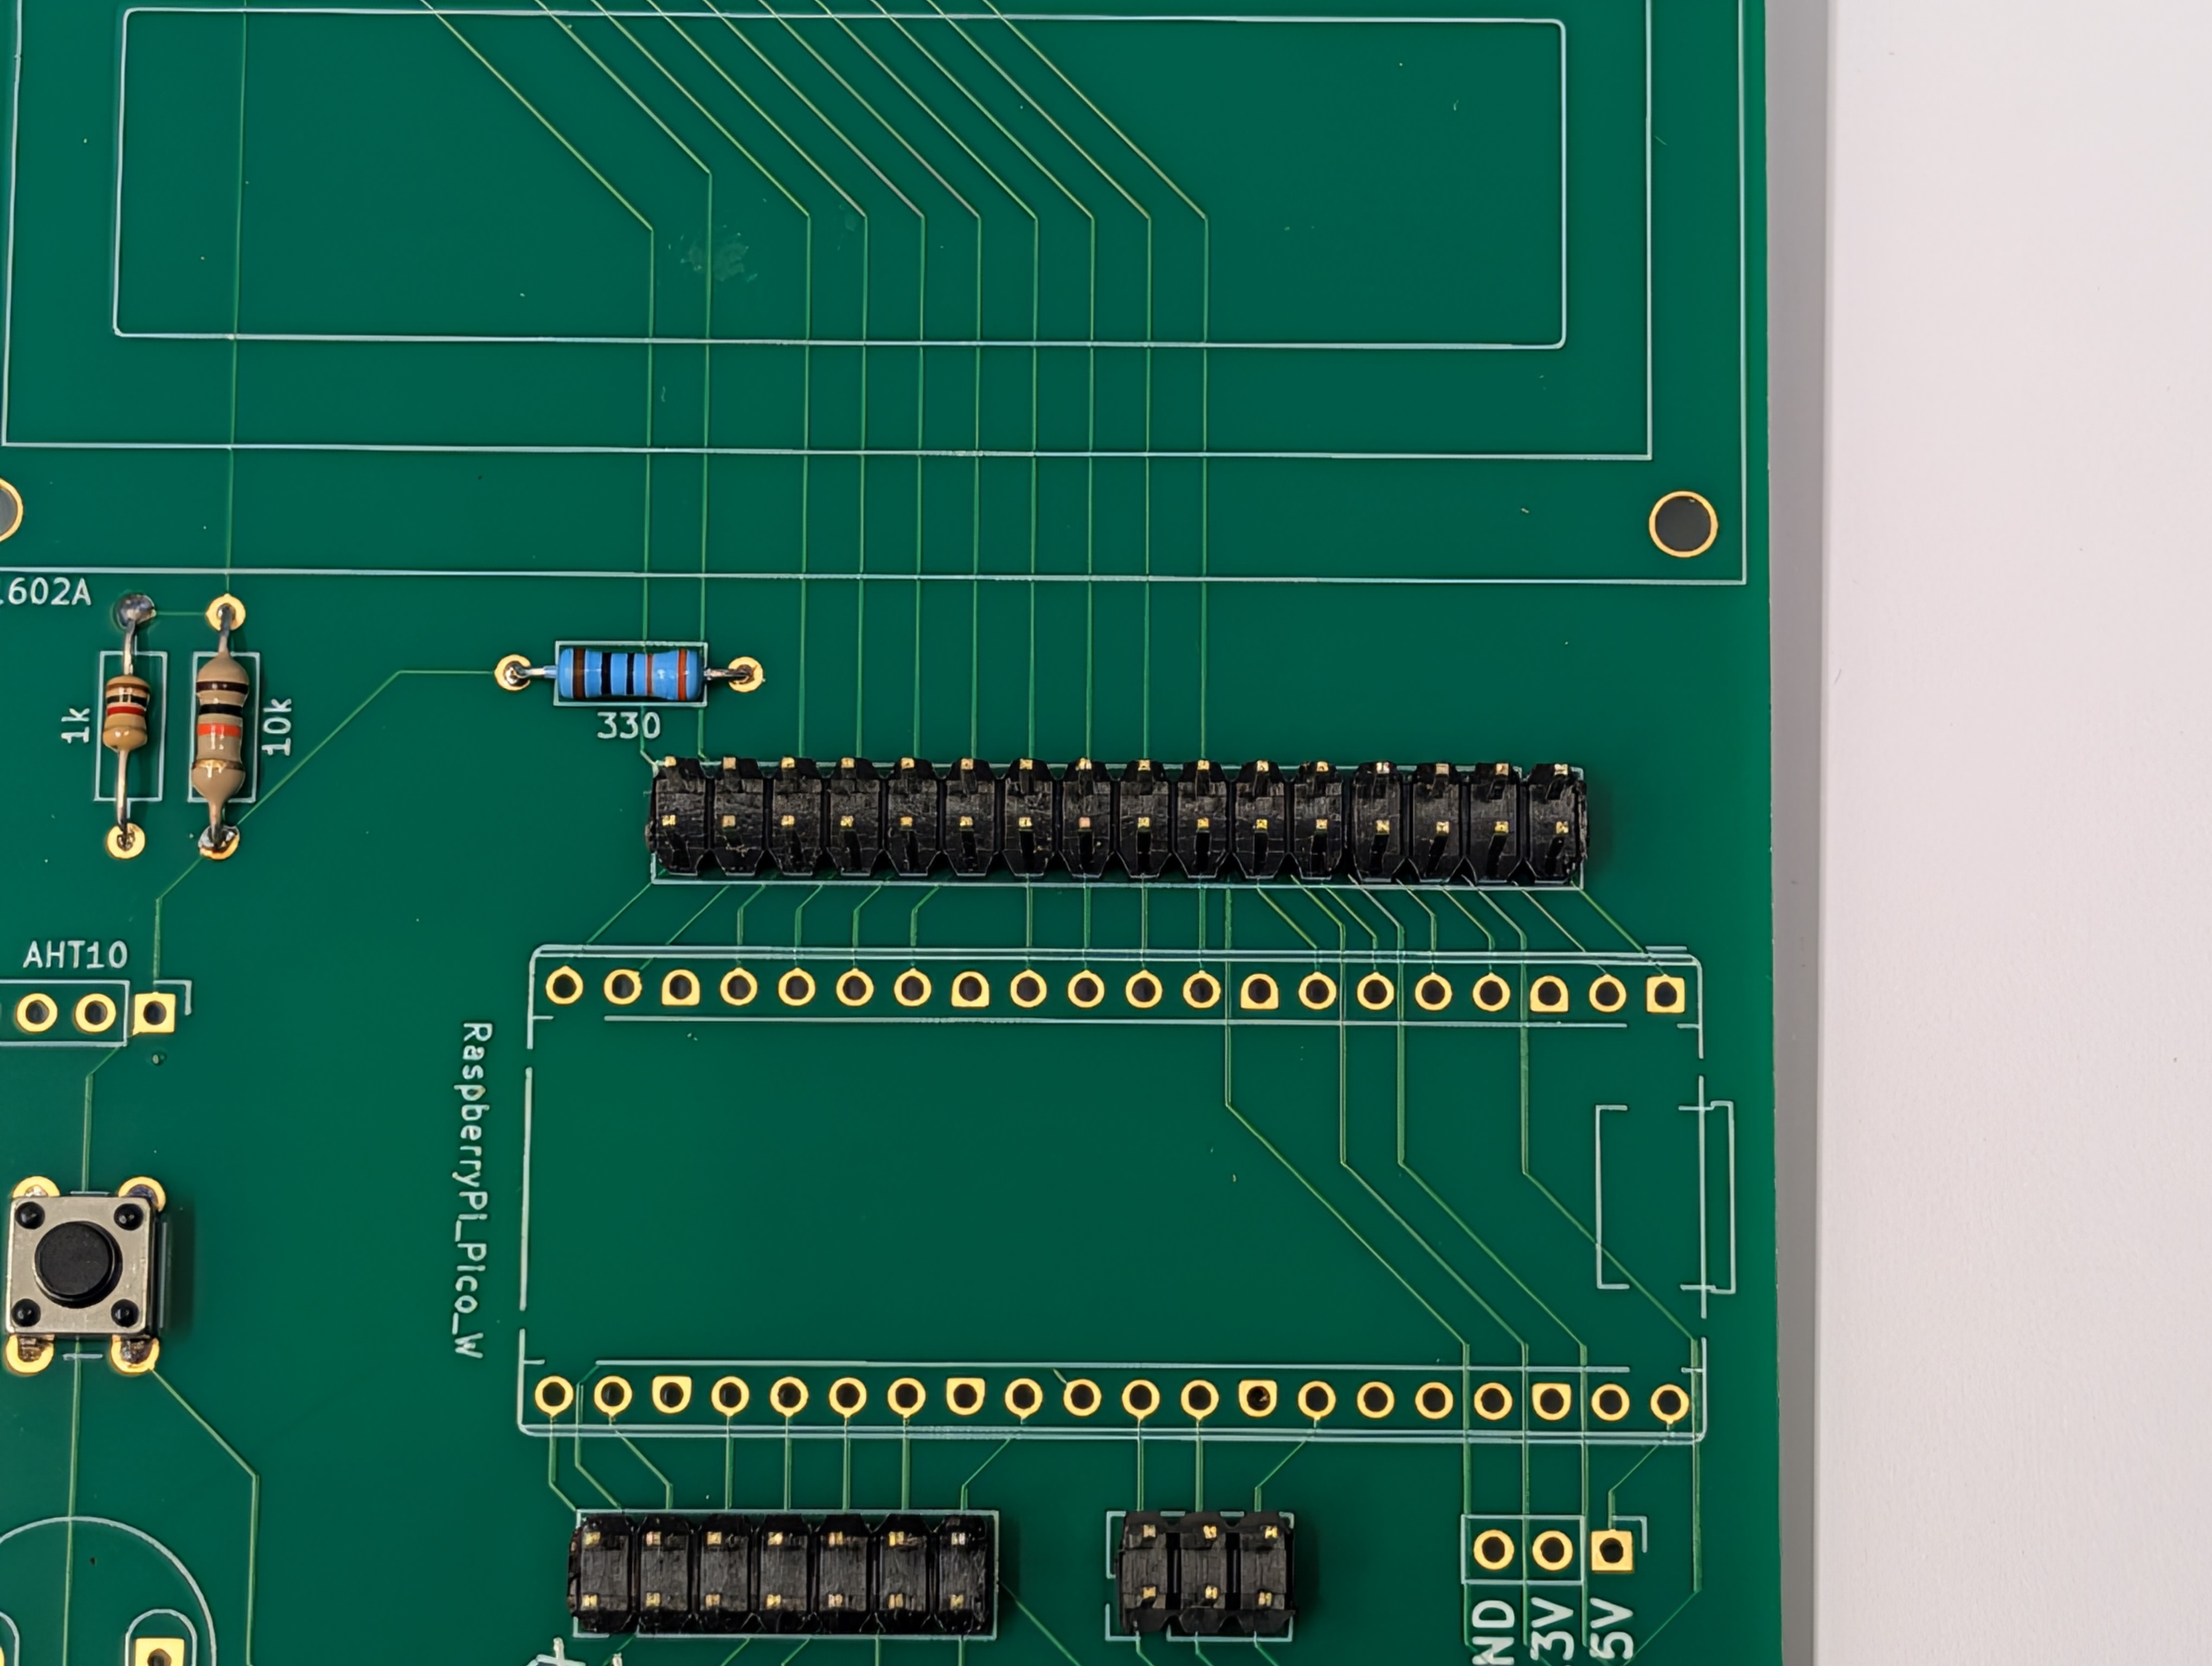
\includegraphics[width=0.75\textwidth]{pictures_of_construction/instruction_step_50.jpg}
\end{figure}

\begin{figure}[H]
    \centering
    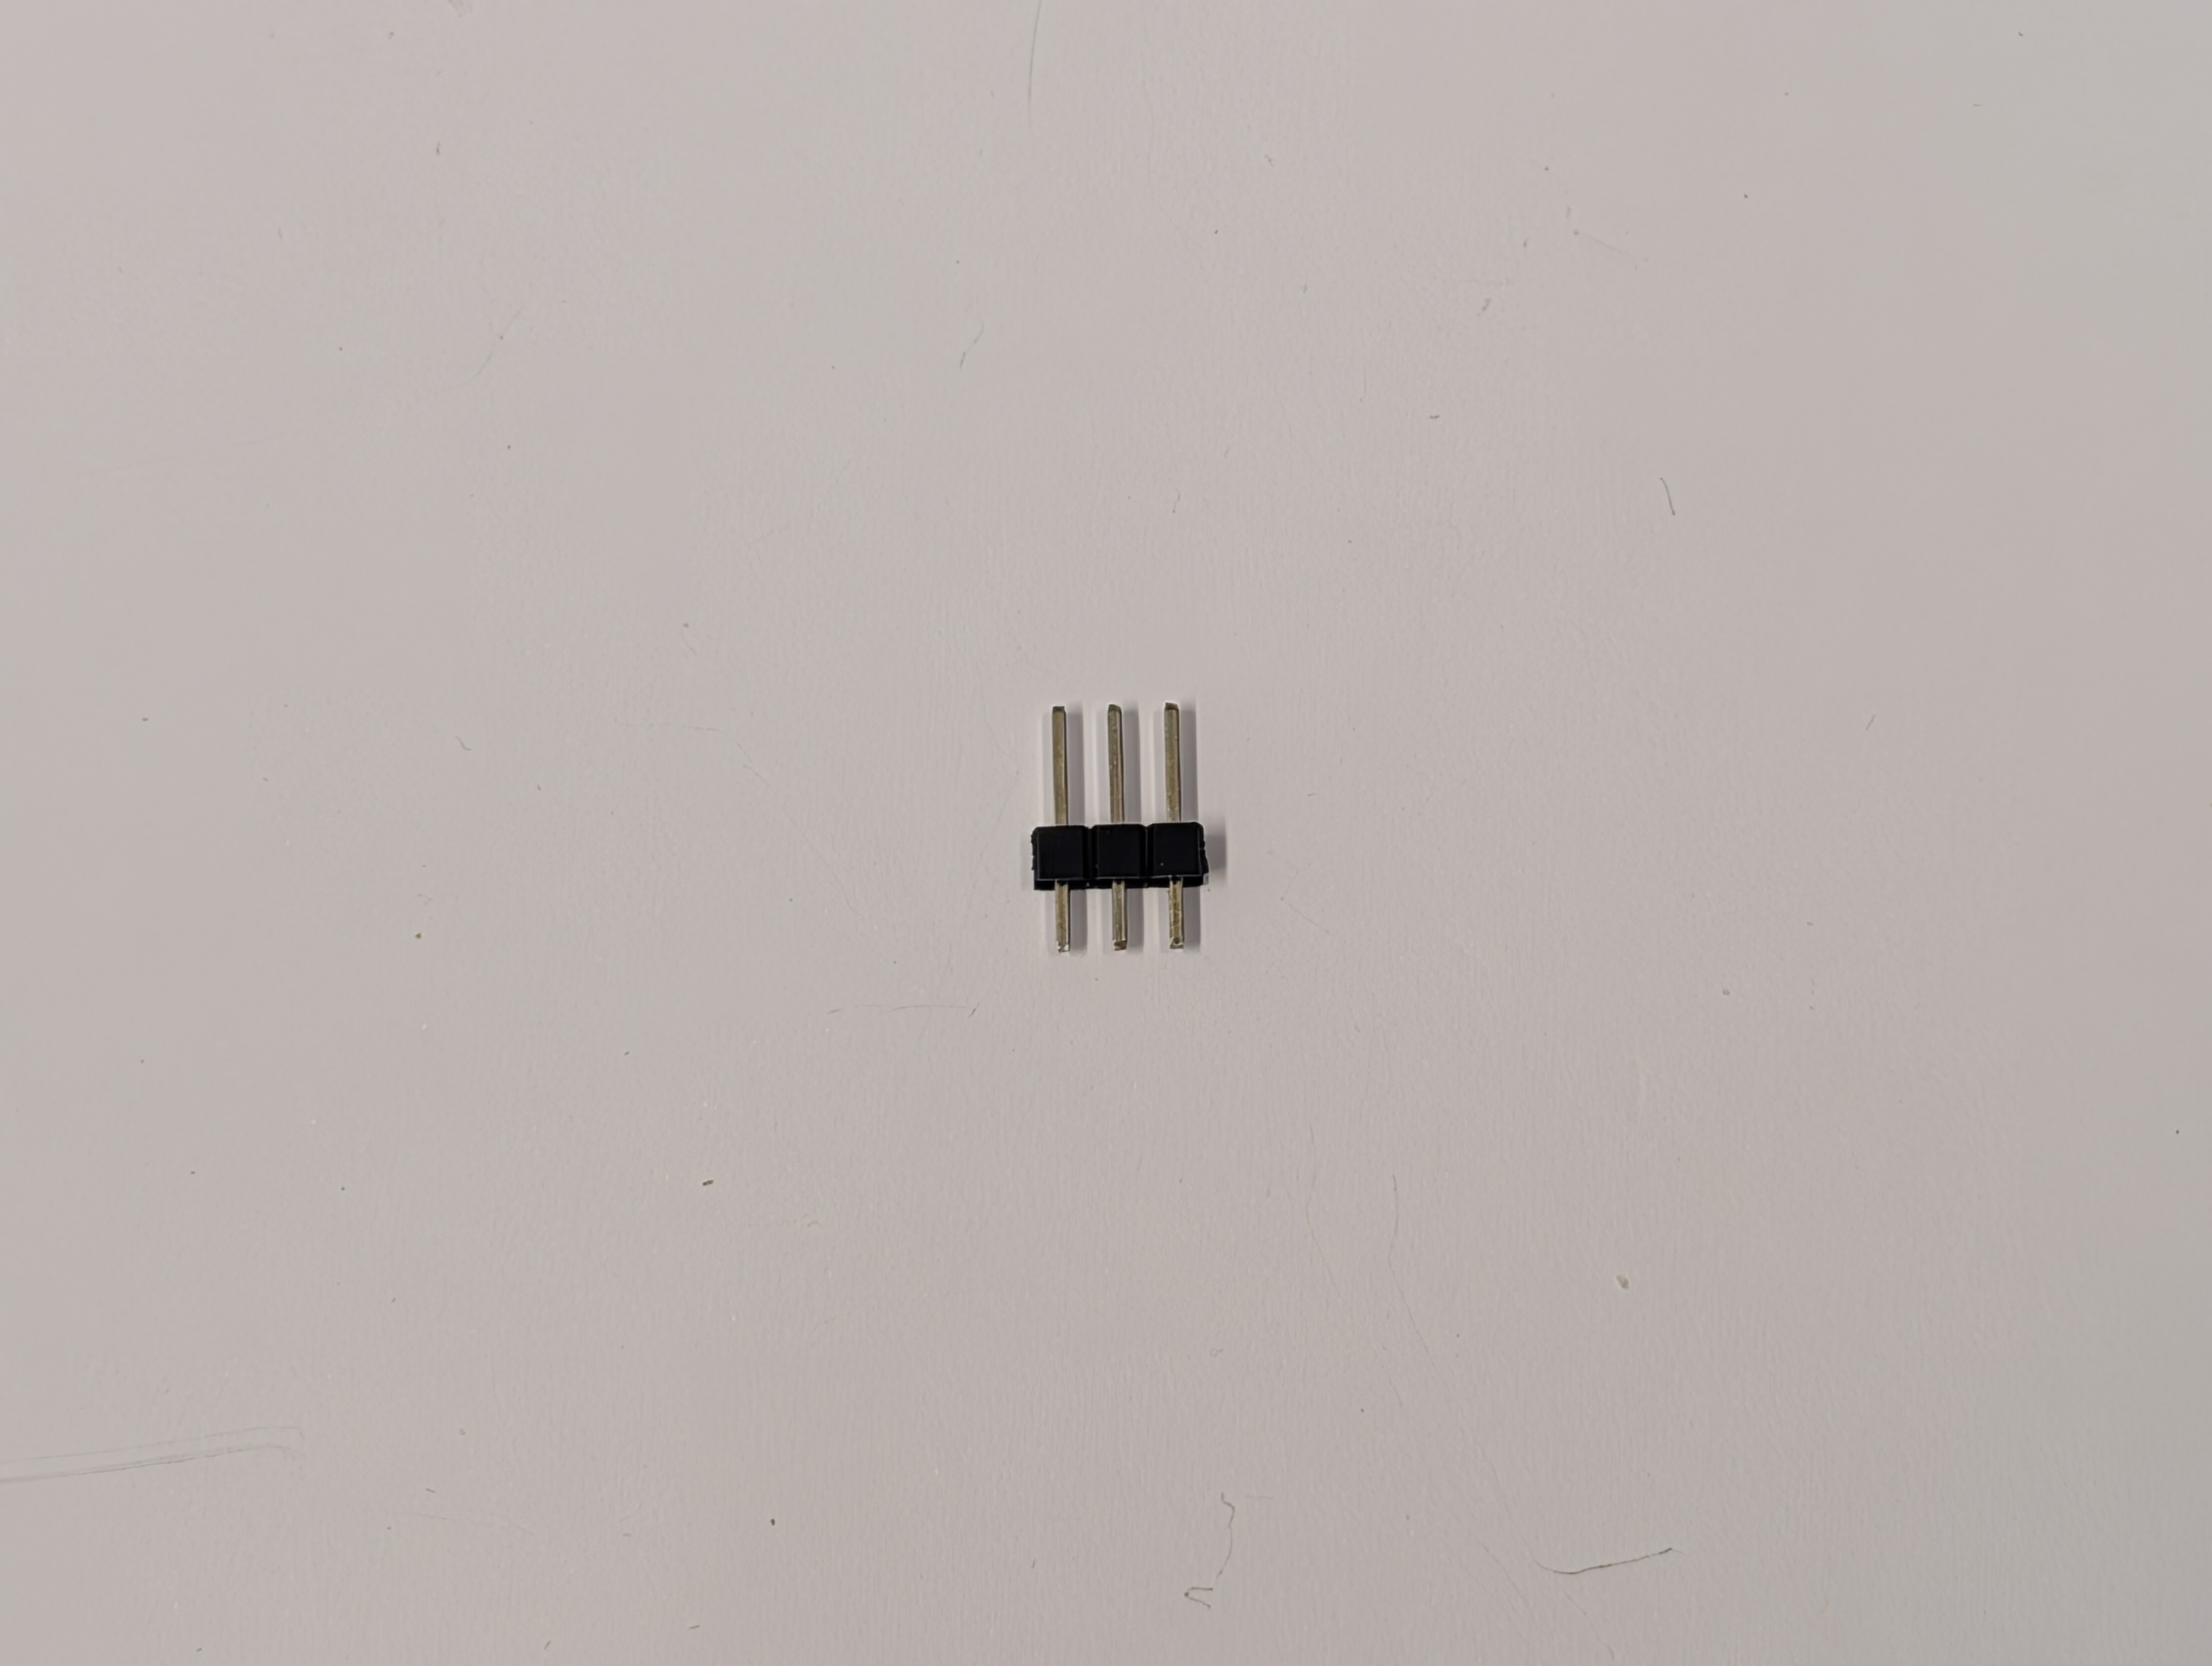
\includegraphics[width=0.75\textwidth]{pictures_of_construction/instruction_step_51.jpg}
\end{figure}

\begin{figure}[H]
    \centering
    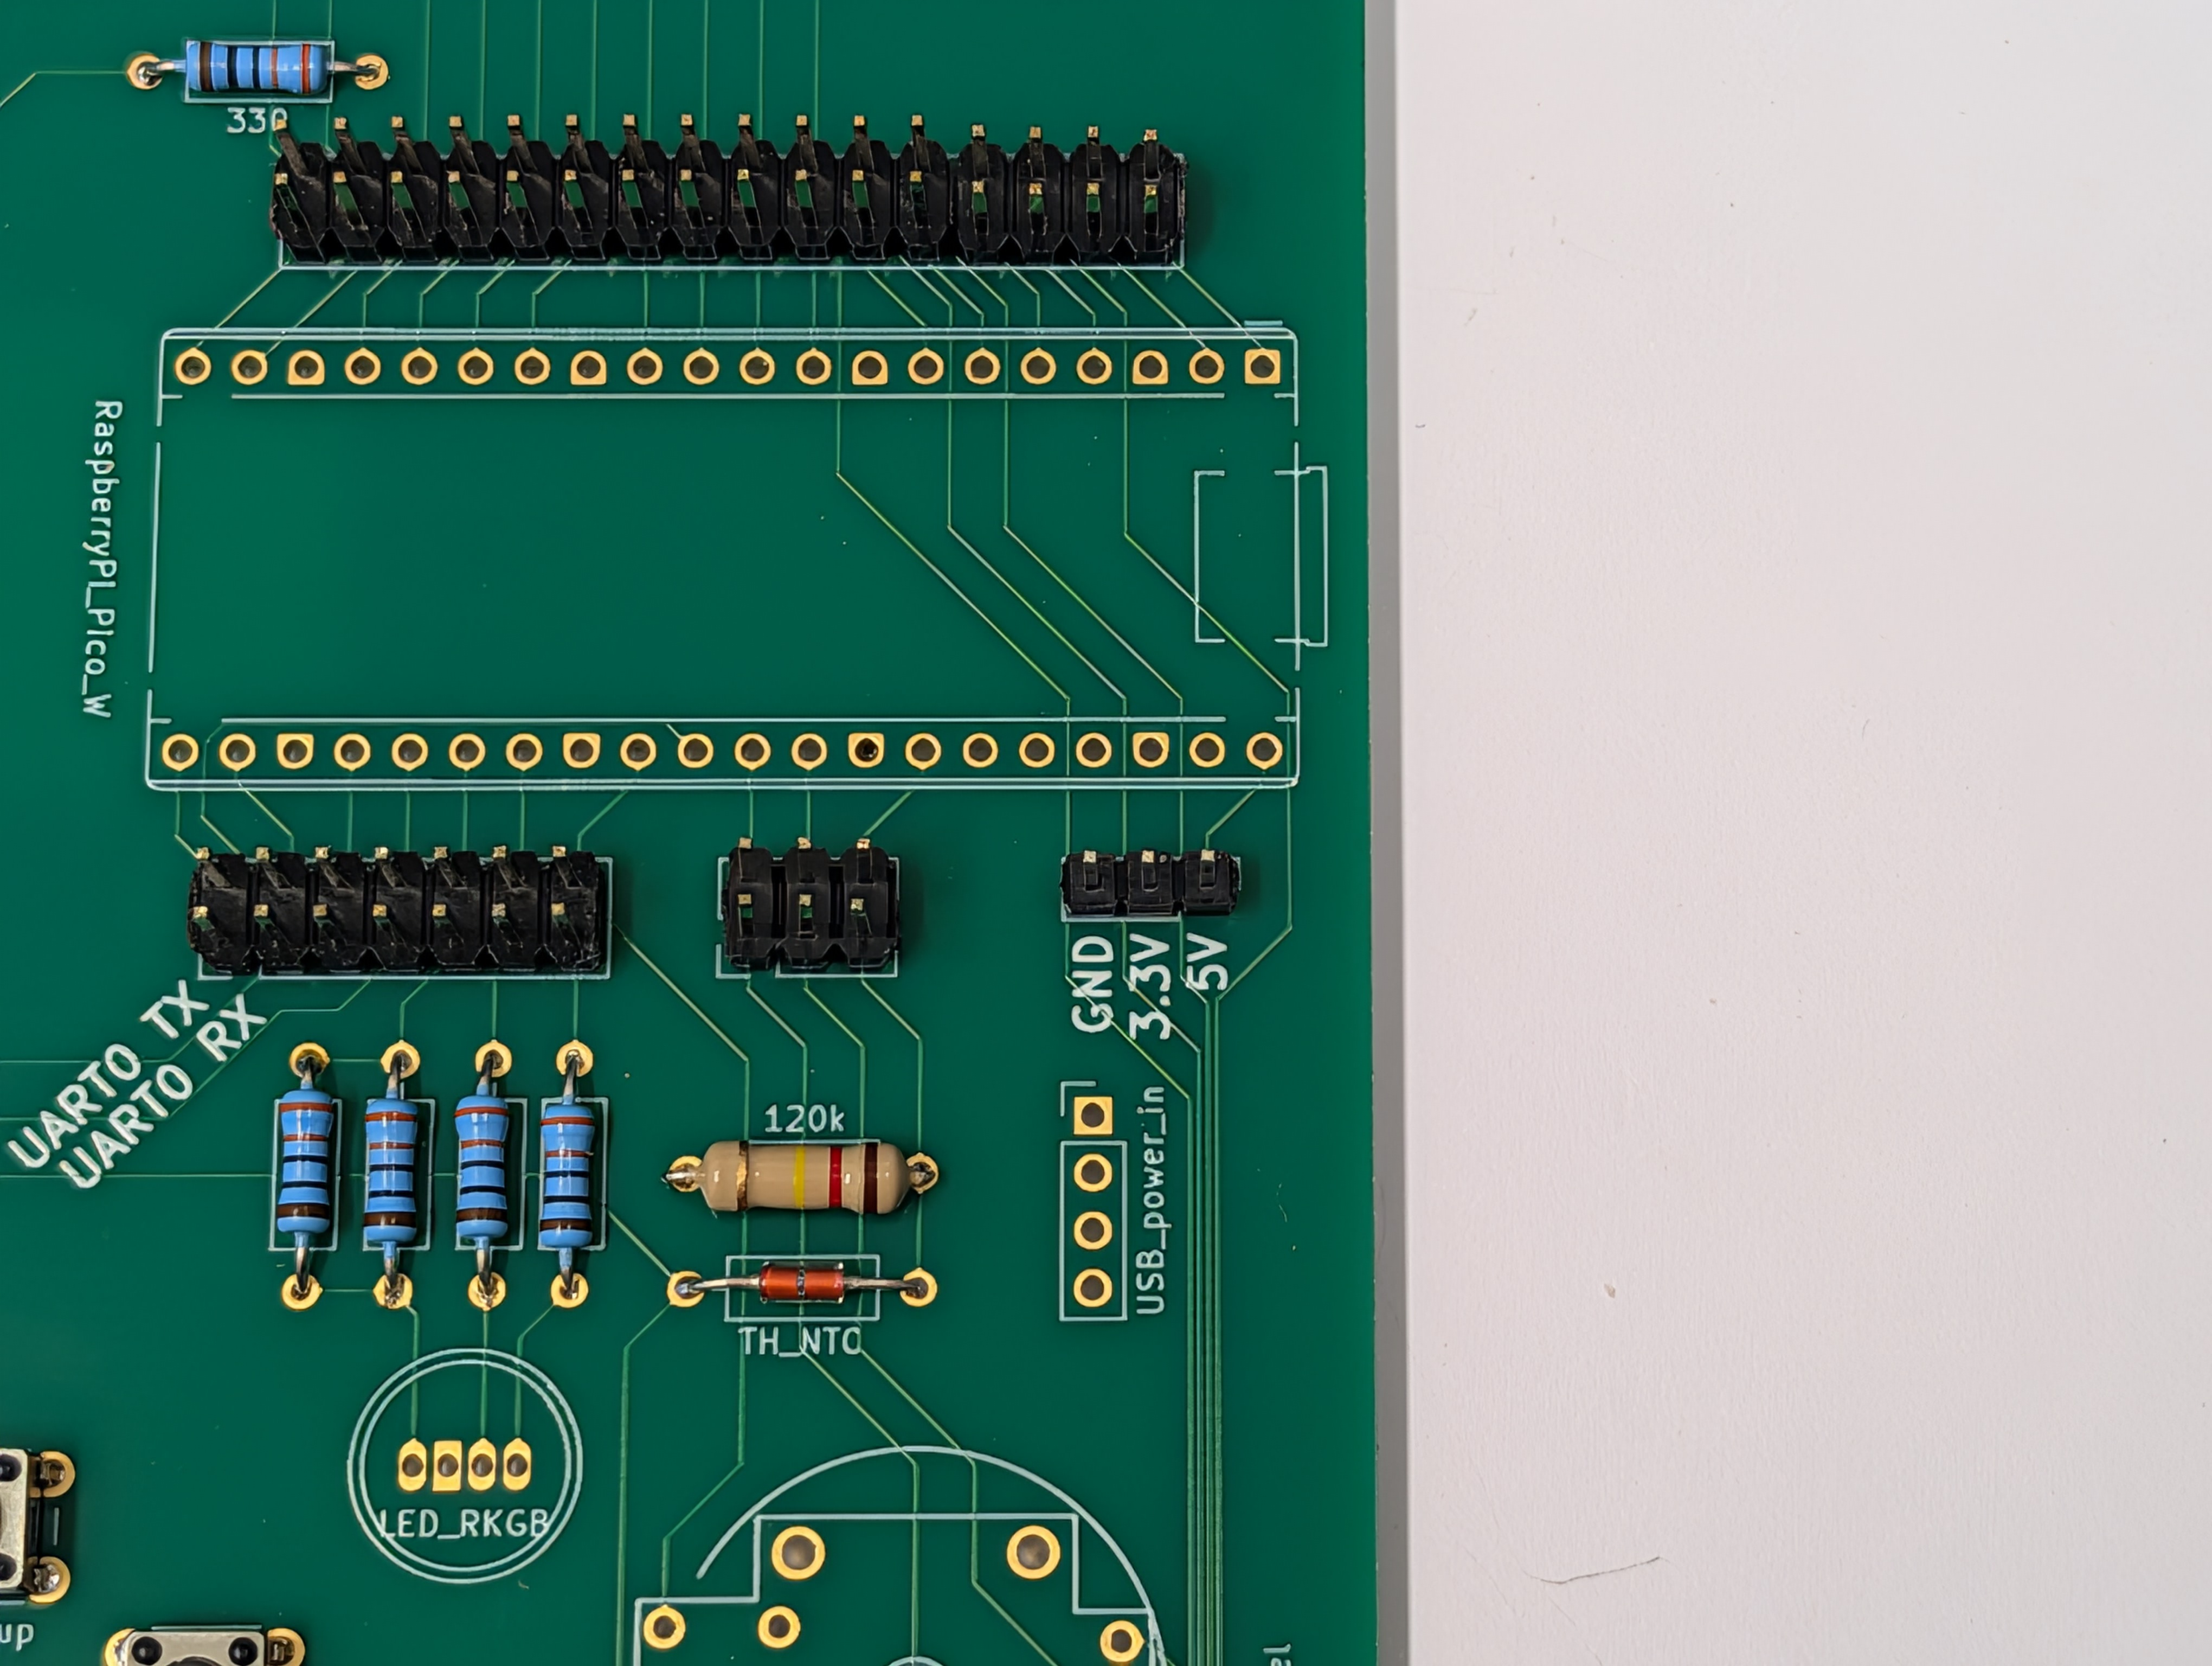
\includegraphics[width=0.75\textwidth]{pictures_of_construction/instruction_step_52.jpg}
\end{figure}

\subsection*{8. USB-C-Breakout-Board einbauen}

Jetzt kommt das vorbereitete USB-C-Breakout-Board auf die große Platine.

So geht’s:
\begin{enumerate}
    \item Stecke es an die richtige Stelle auf der rechten Seite der Platine.
    \item Der USB-Anschluss soll nach außen zeigen und gut sichtbar sein.
    \item Löte zuerst einen Pin.
    \item Prüfe, ob das Board gerade und parallel zur Platine steht.
    \item Löte dann alle Pins.
\end{enumerate}

\textbf{Achtung:}\\
Die Pins sind härter als normale Drahtenden.\\
Benutze dafür einen \textbf{größeren Seitenschneider}.

\begin{figure}[H]
    \centering
    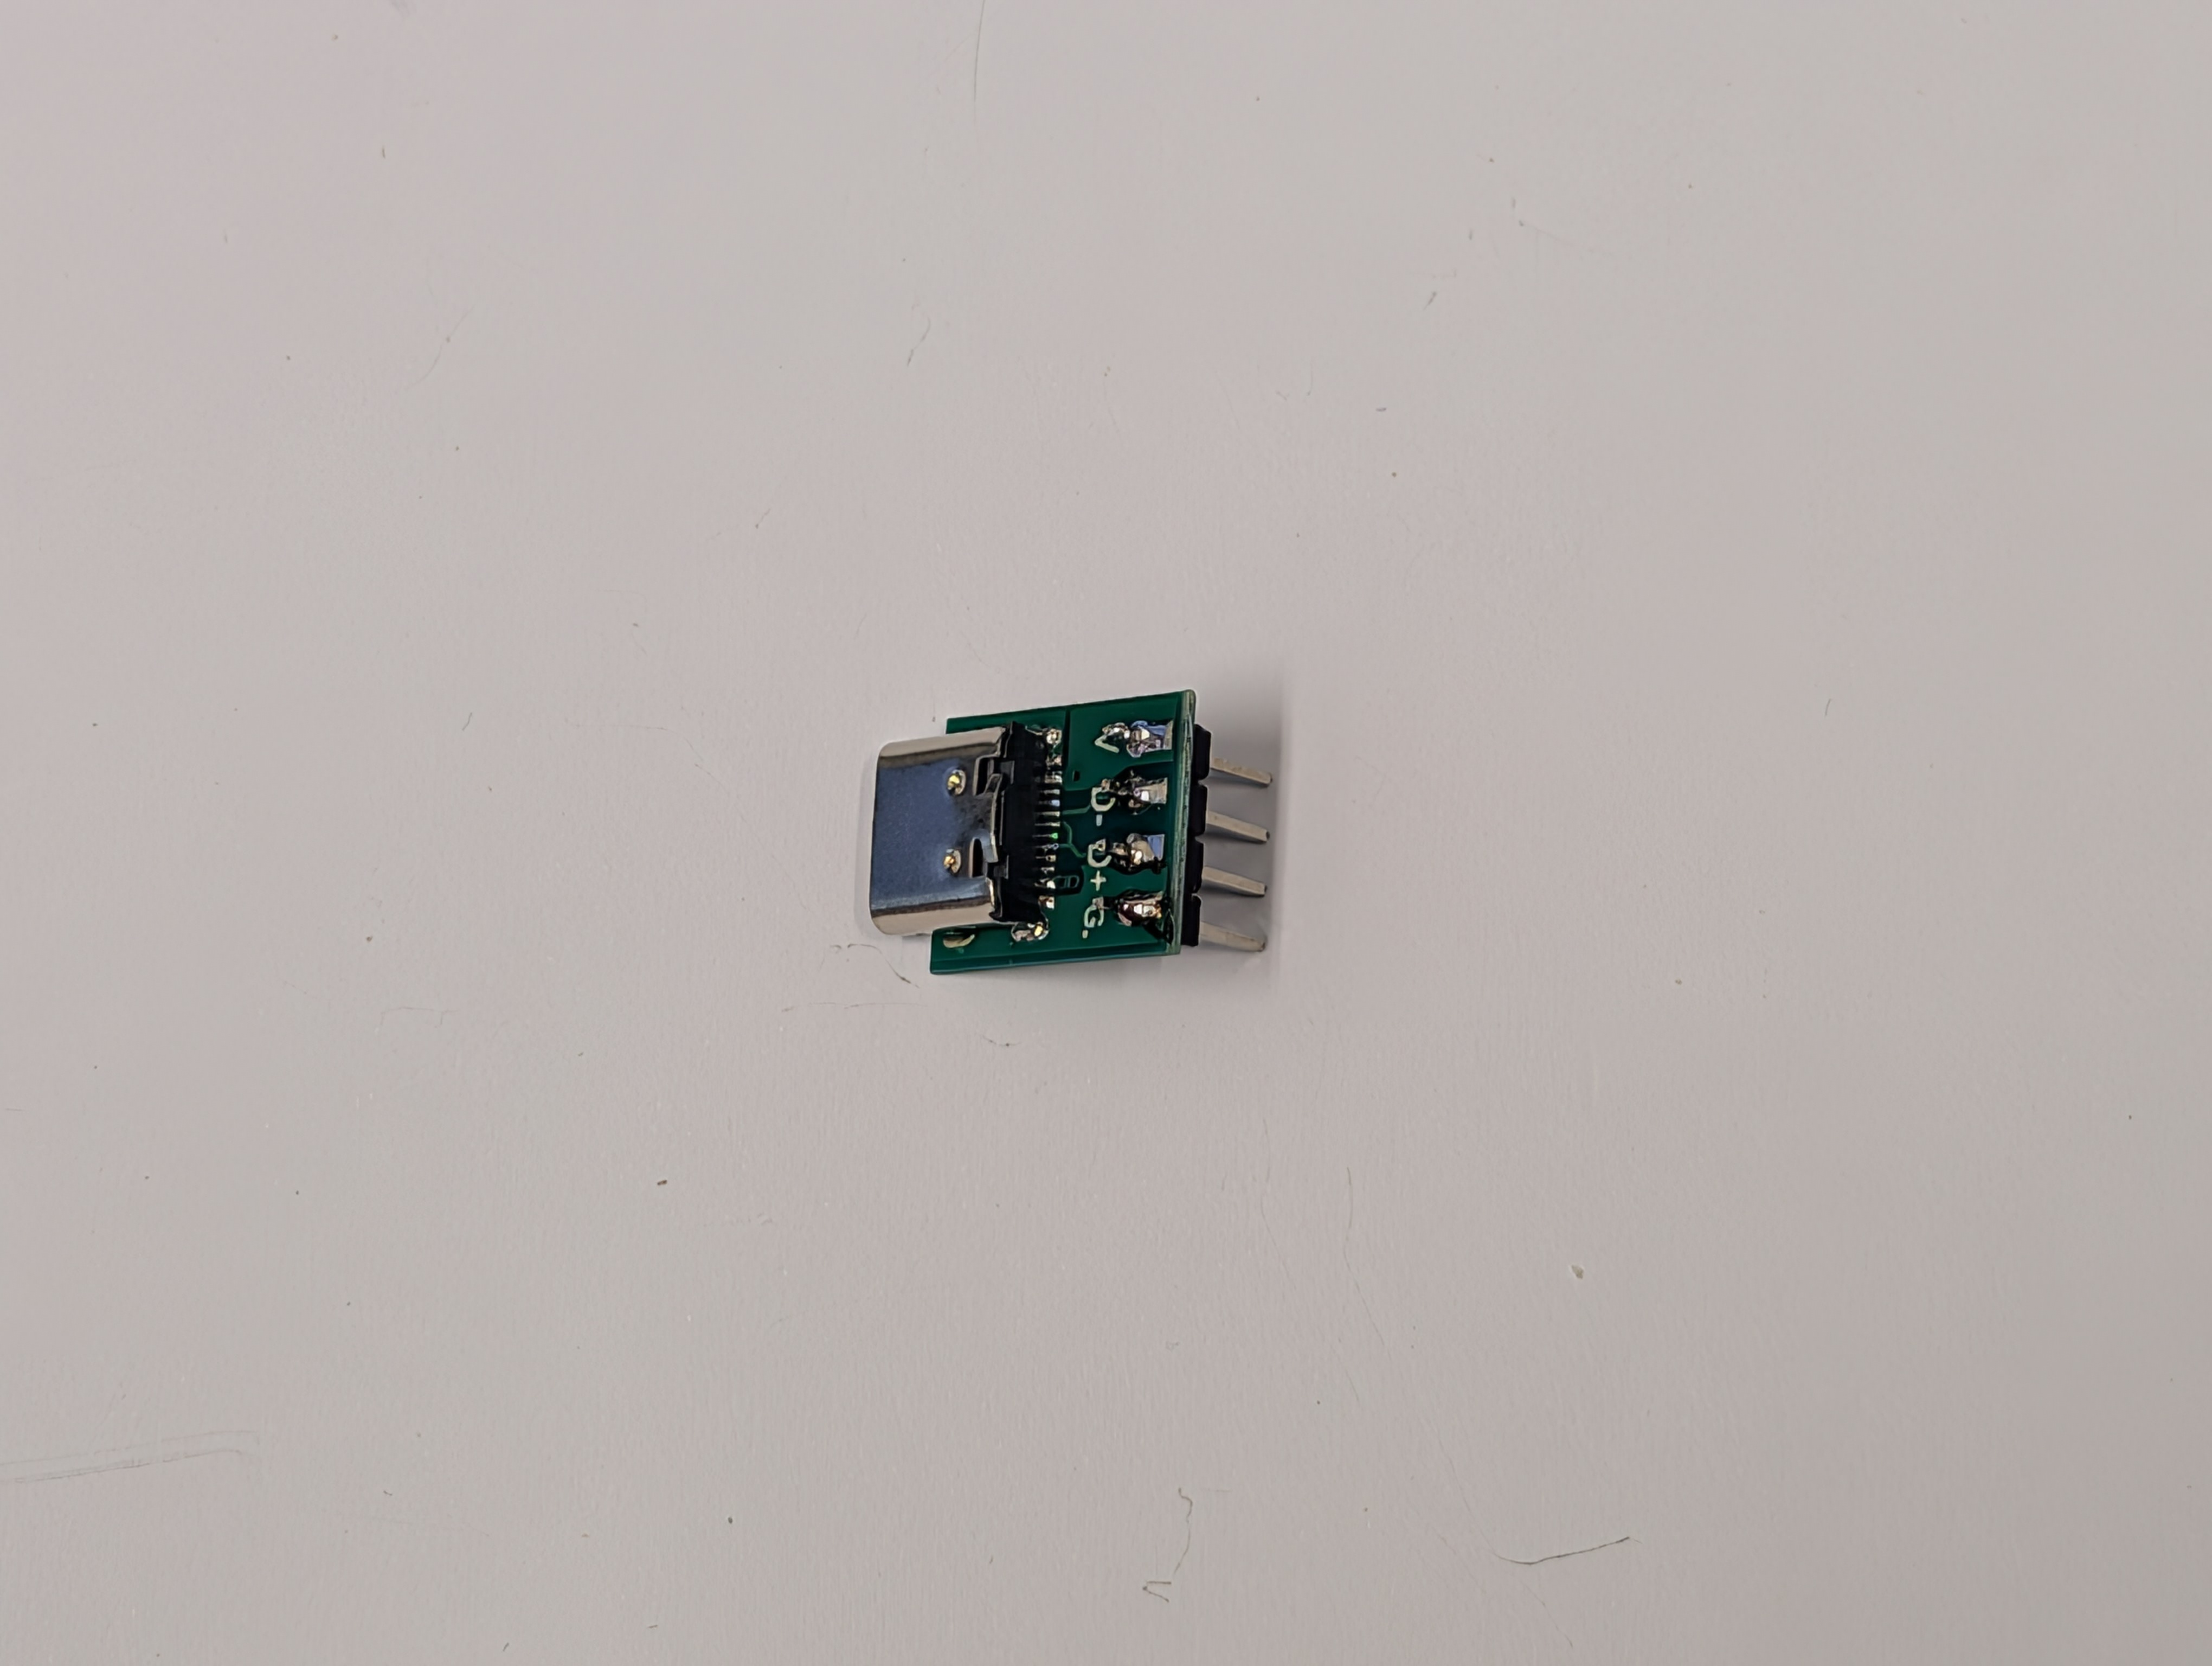
\includegraphics[width=0.75\textwidth]{pictures_of_construction/instruction_step_53.jpg}
\end{figure}

\begin{figure}[H]
    \centering
    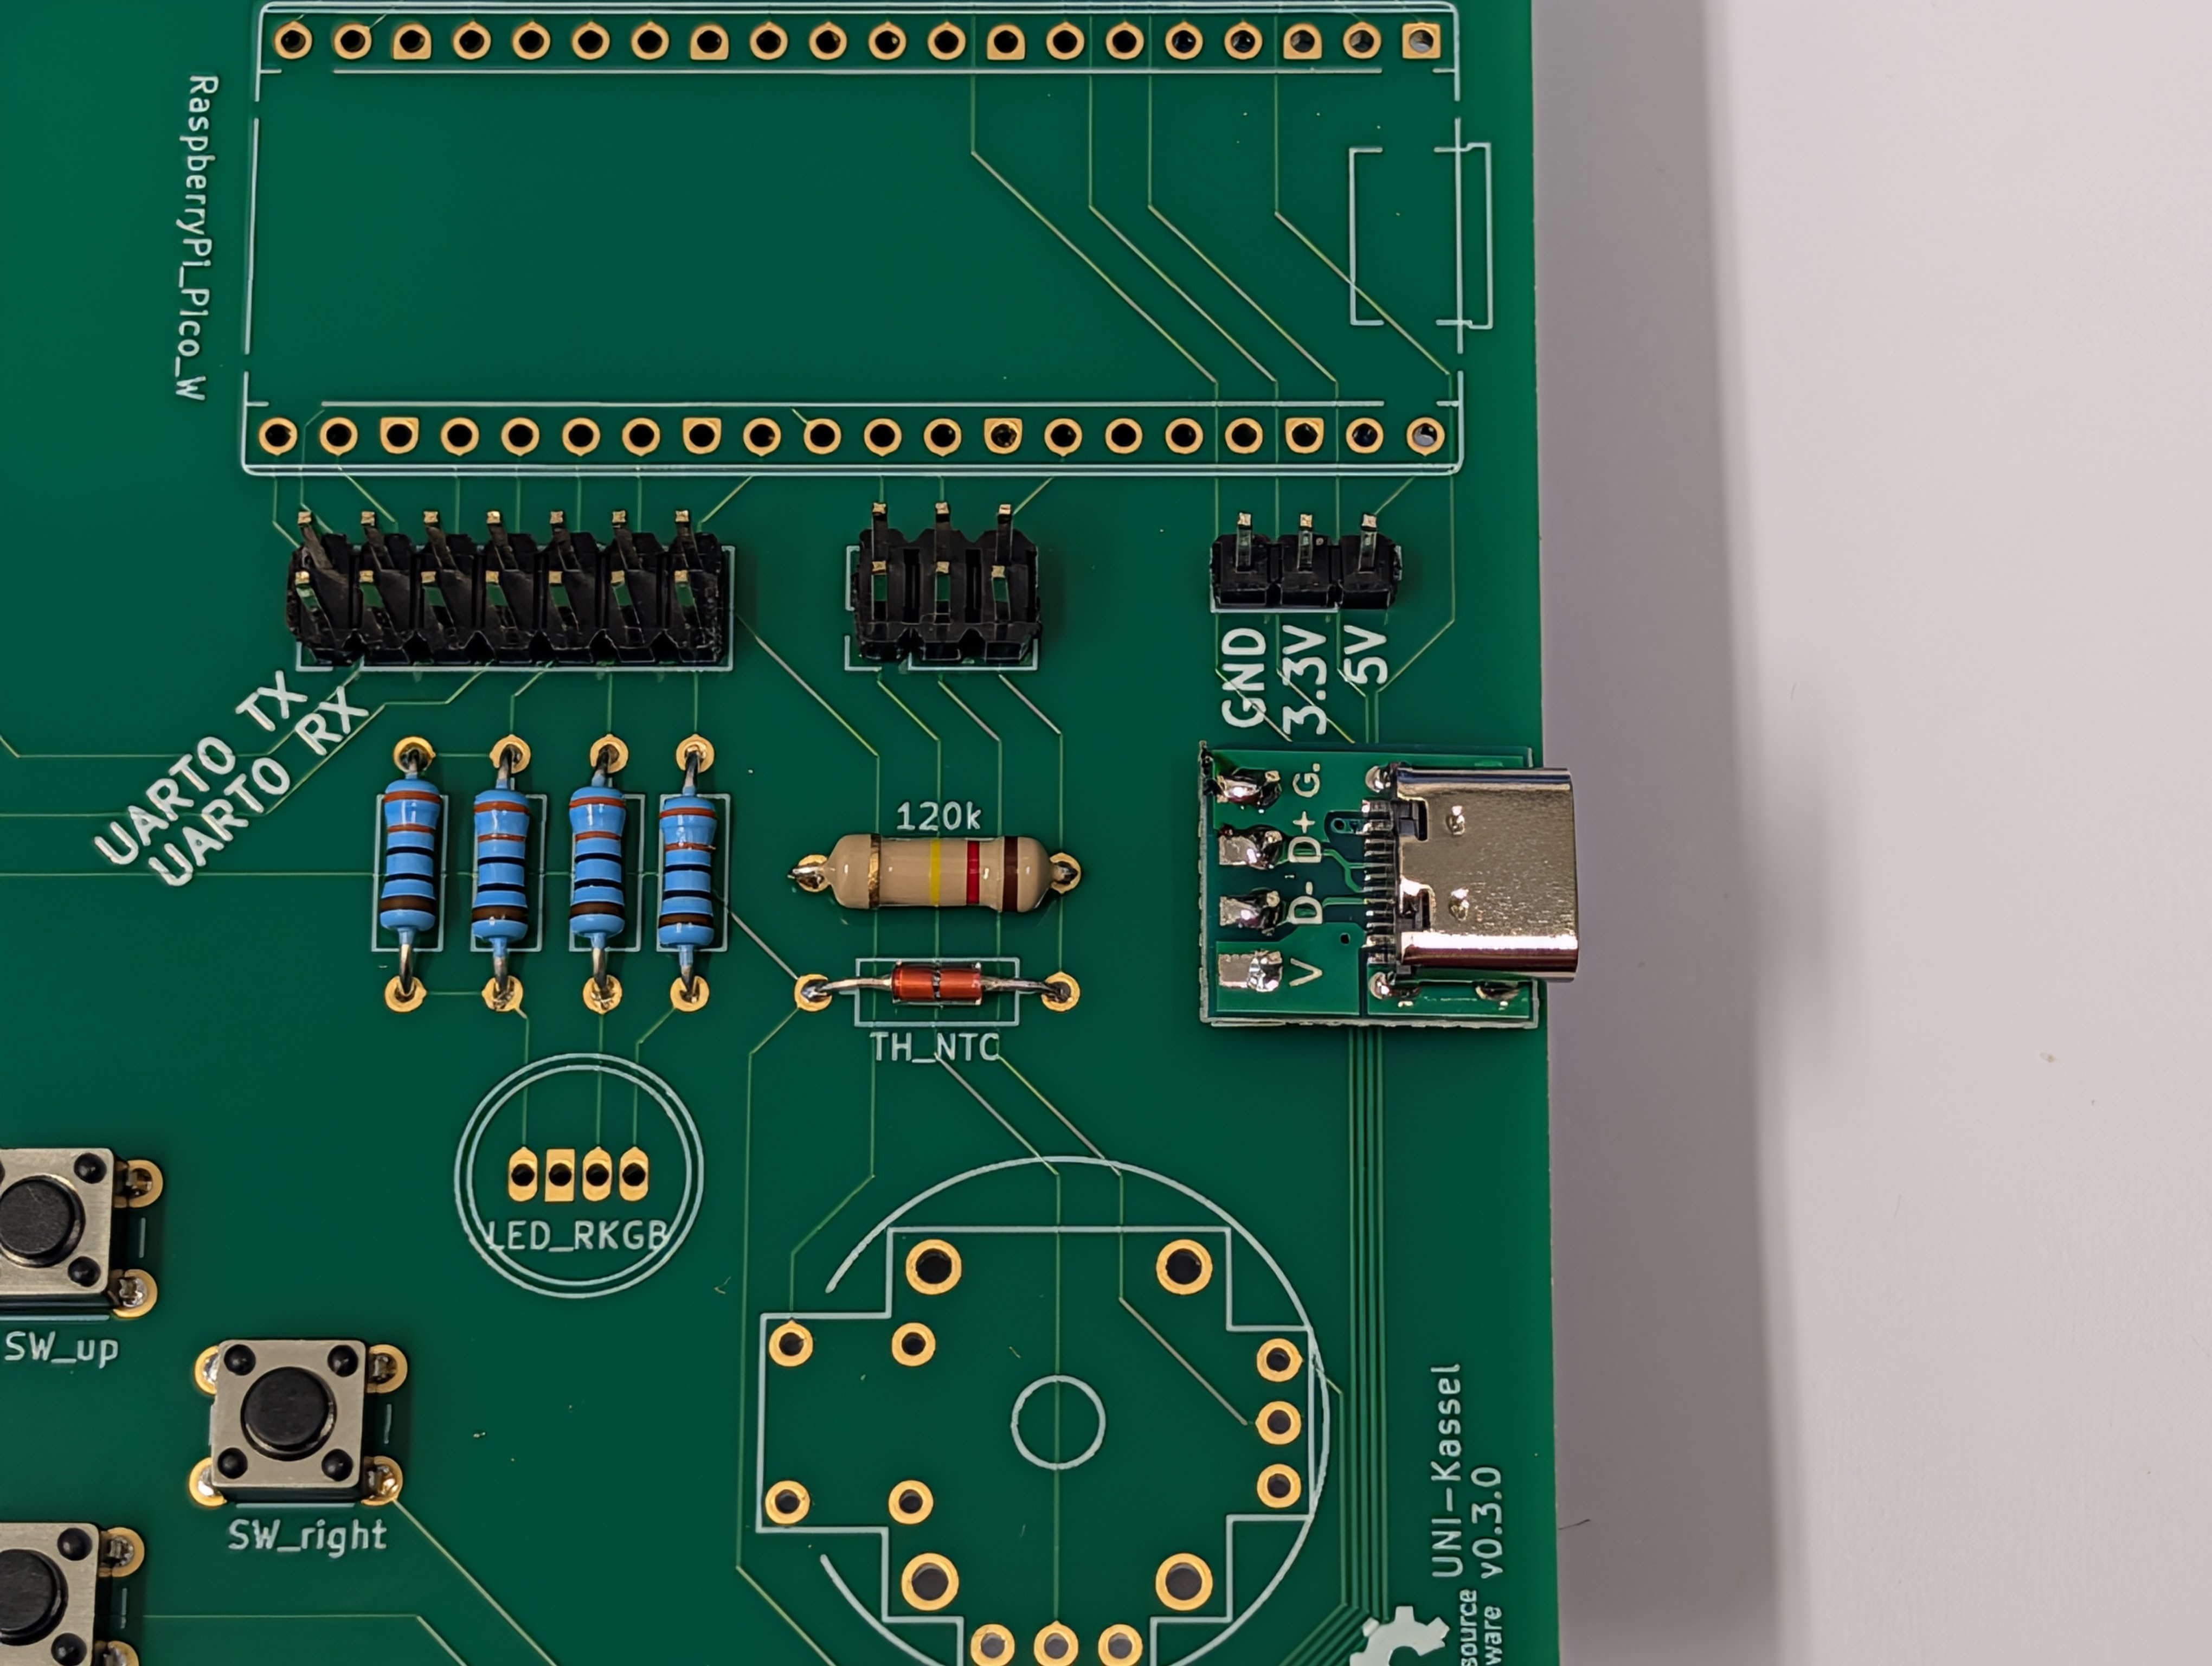
\includegraphics[width=0.75\textwidth]{pictures_of_construction/instruction_step_54.jpg}
\end{figure}

\begin{figure}[H]
    \centering
    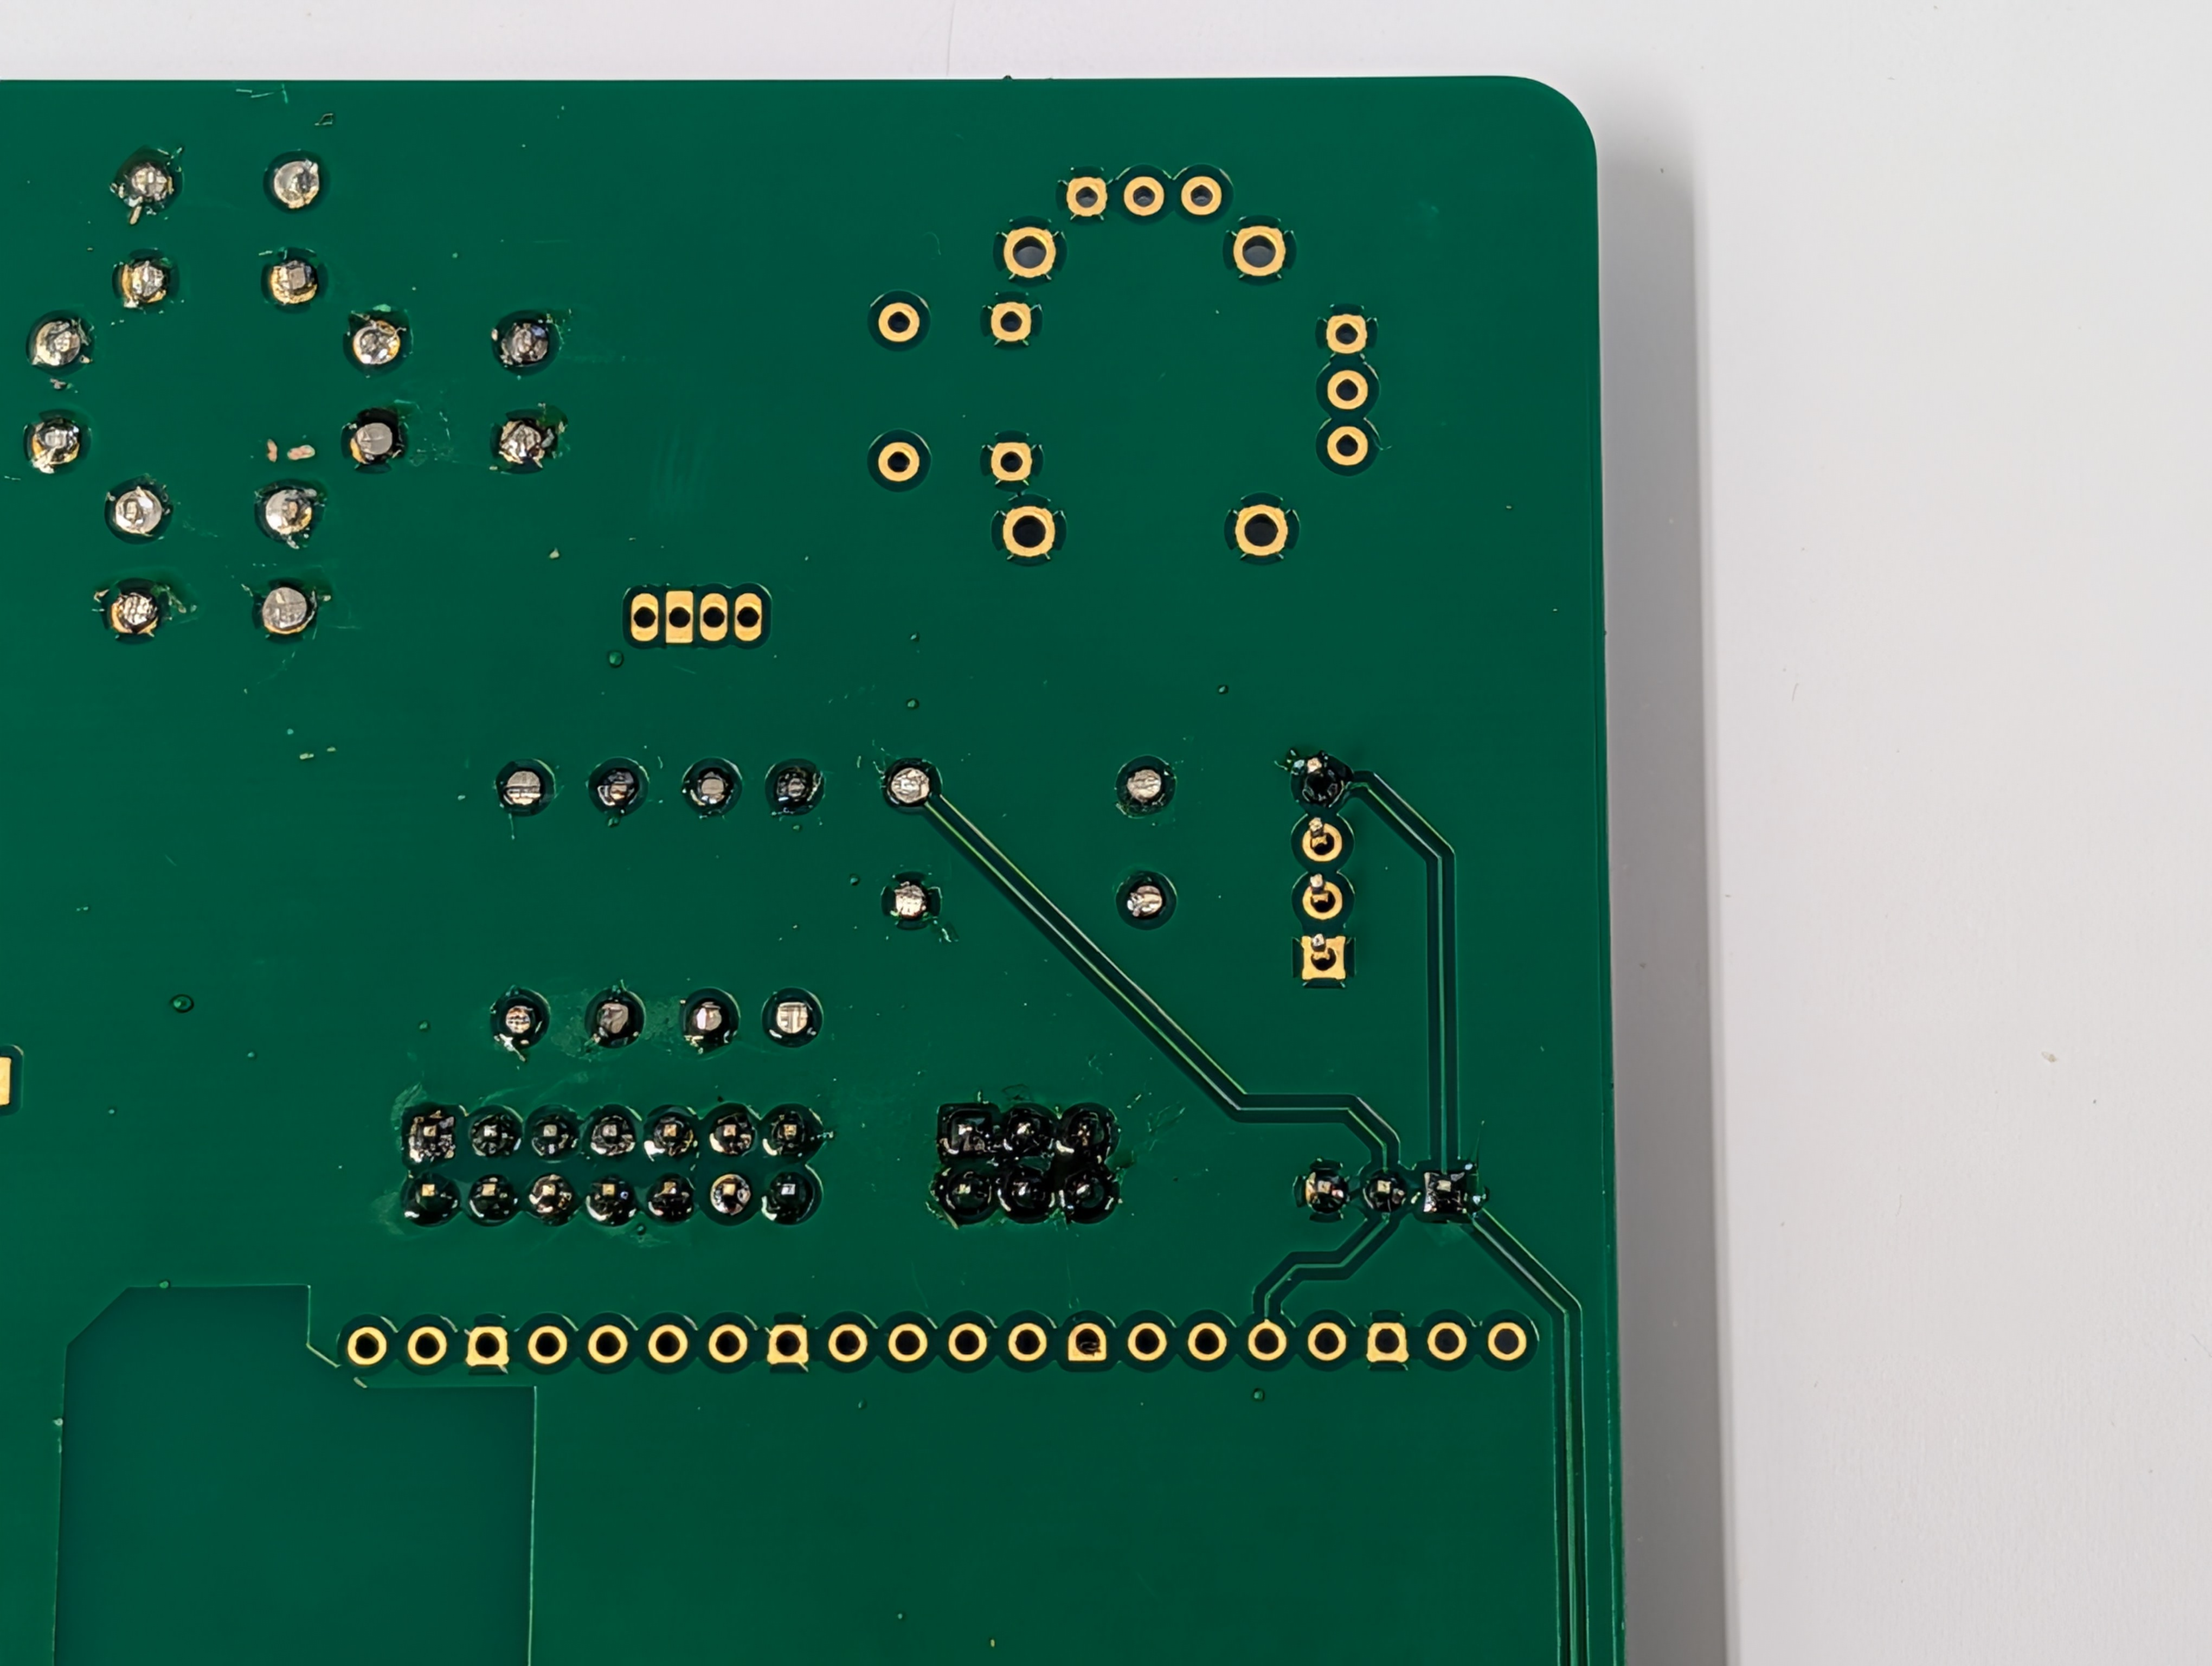
\includegraphics[width=0.75\textwidth]{pictures_of_construction/instruction_step_55.jpg}
\end{figure}

\begin{figure}[H]
    \centering
    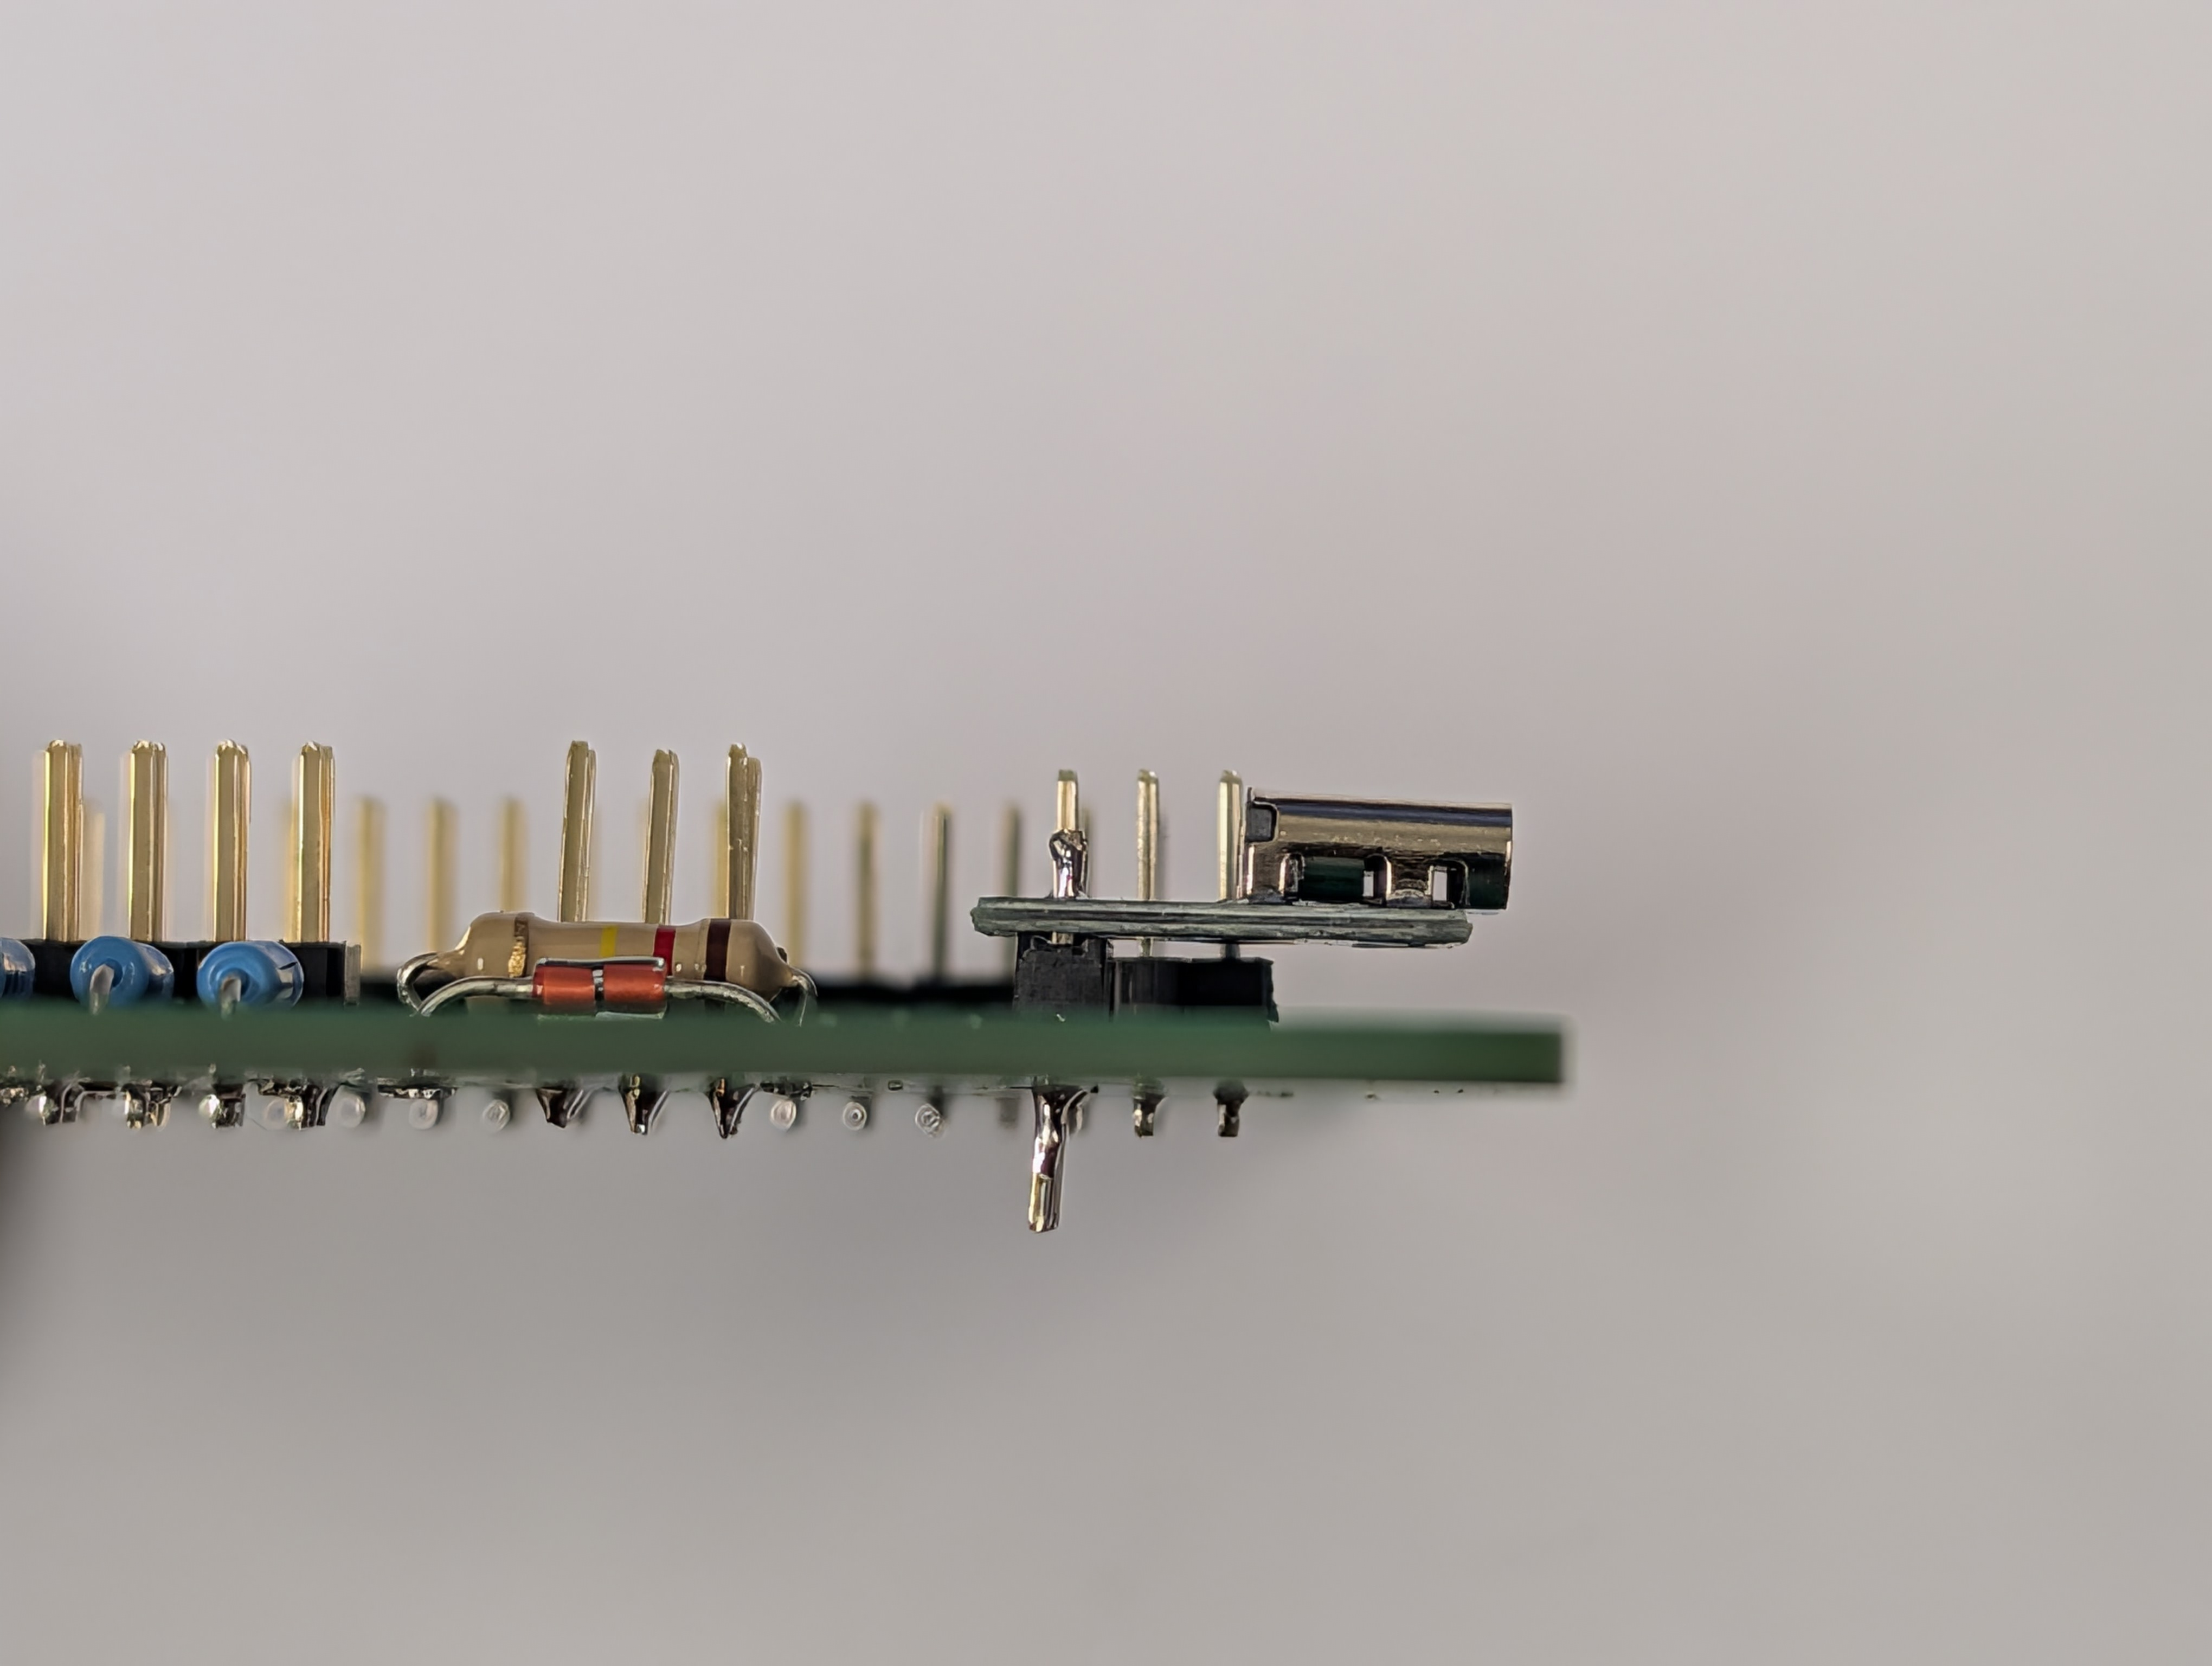
\includegraphics[width=0.75\textwidth]{pictures_of_construction/instruction_step_56.jpg}
\end{figure}

\subsection*{9. AHT10-Sensor einbauen}

Jetzt kommt der vorbereitete AHT10-Sensor auf die Platine.

So geht’s:
\begin{enumerate}
    \item Setze ihn auf der linken Seite ein.
    \item Die kleinen Bauteile auf dem Sensor sollen sichtbar sein.
    \item Löte zuerst einen Pin.
    \item Richte ihn gerade aus.
    \item Löte alle Pins fest.
\end{enumerate}

Auch hier:
\begin{itemize}
    \item zum Kürzen besser einen größeren Schneider benutzen
\end{itemize}

\begin{figure}[H]
    \centering
    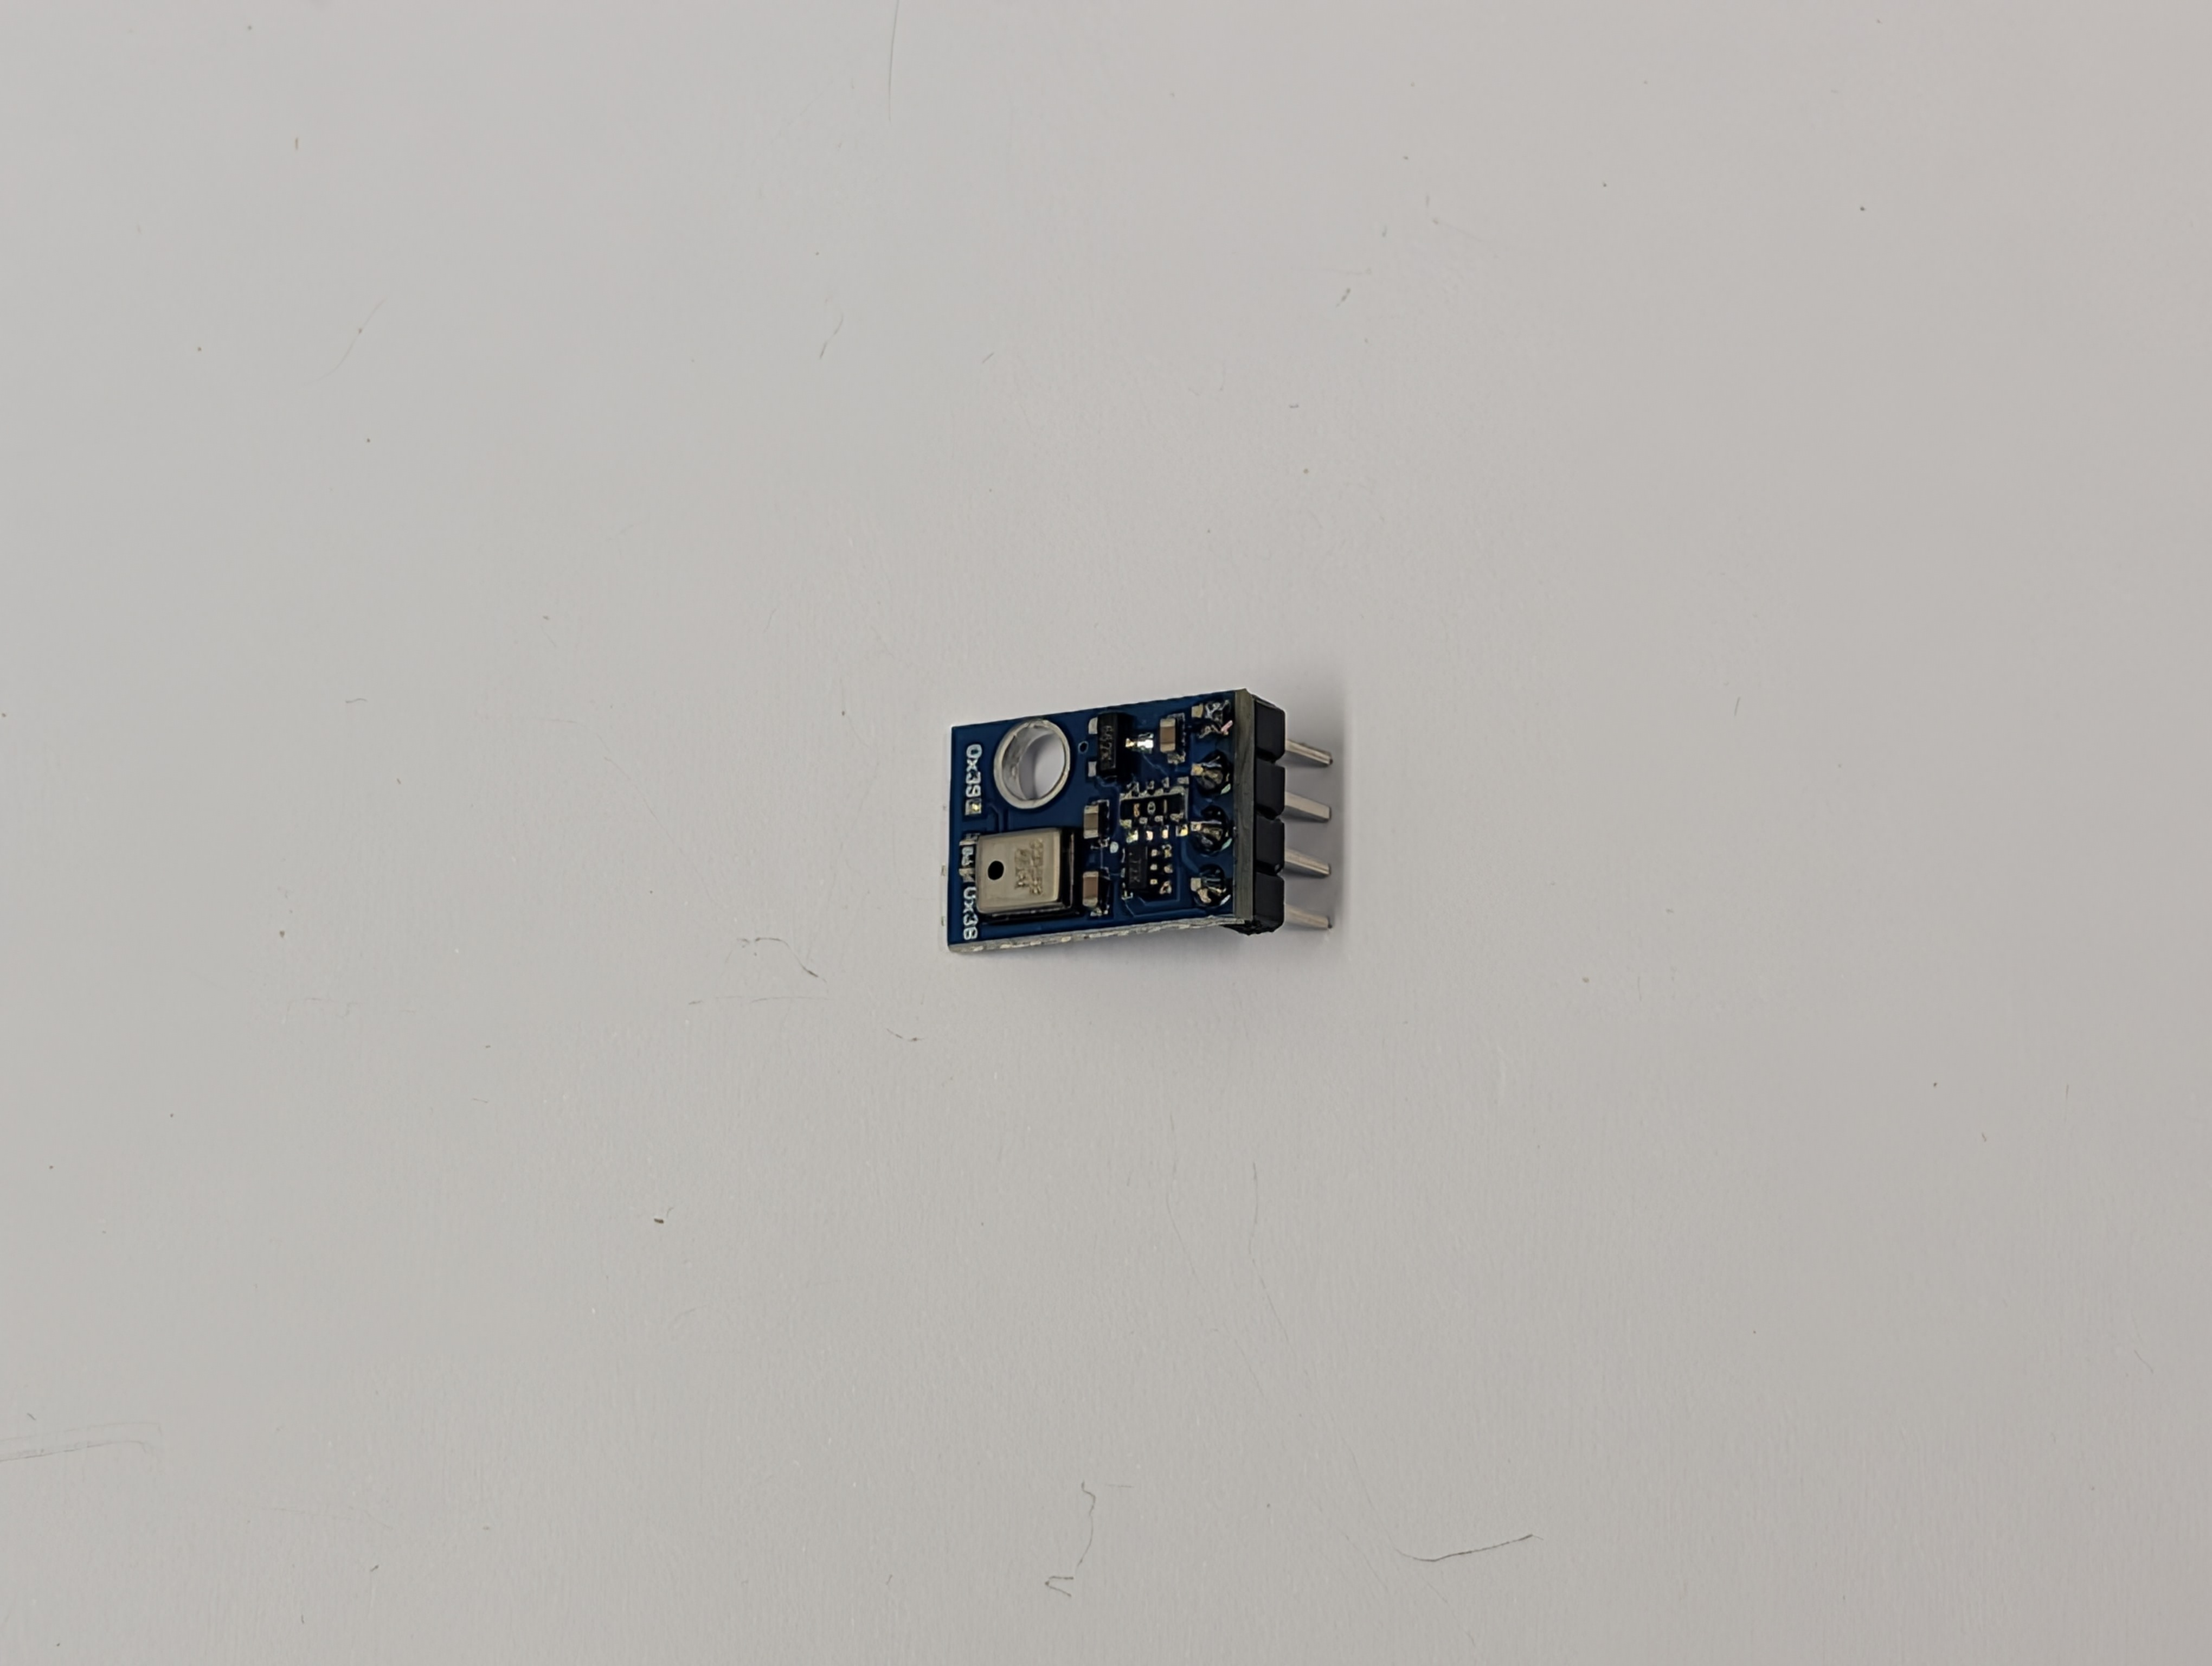
\includegraphics[width=0.75\textwidth]{pictures_of_construction/instruction_step_57.jpg}
\end{figure}

\begin{figure}[H]
    \centering
    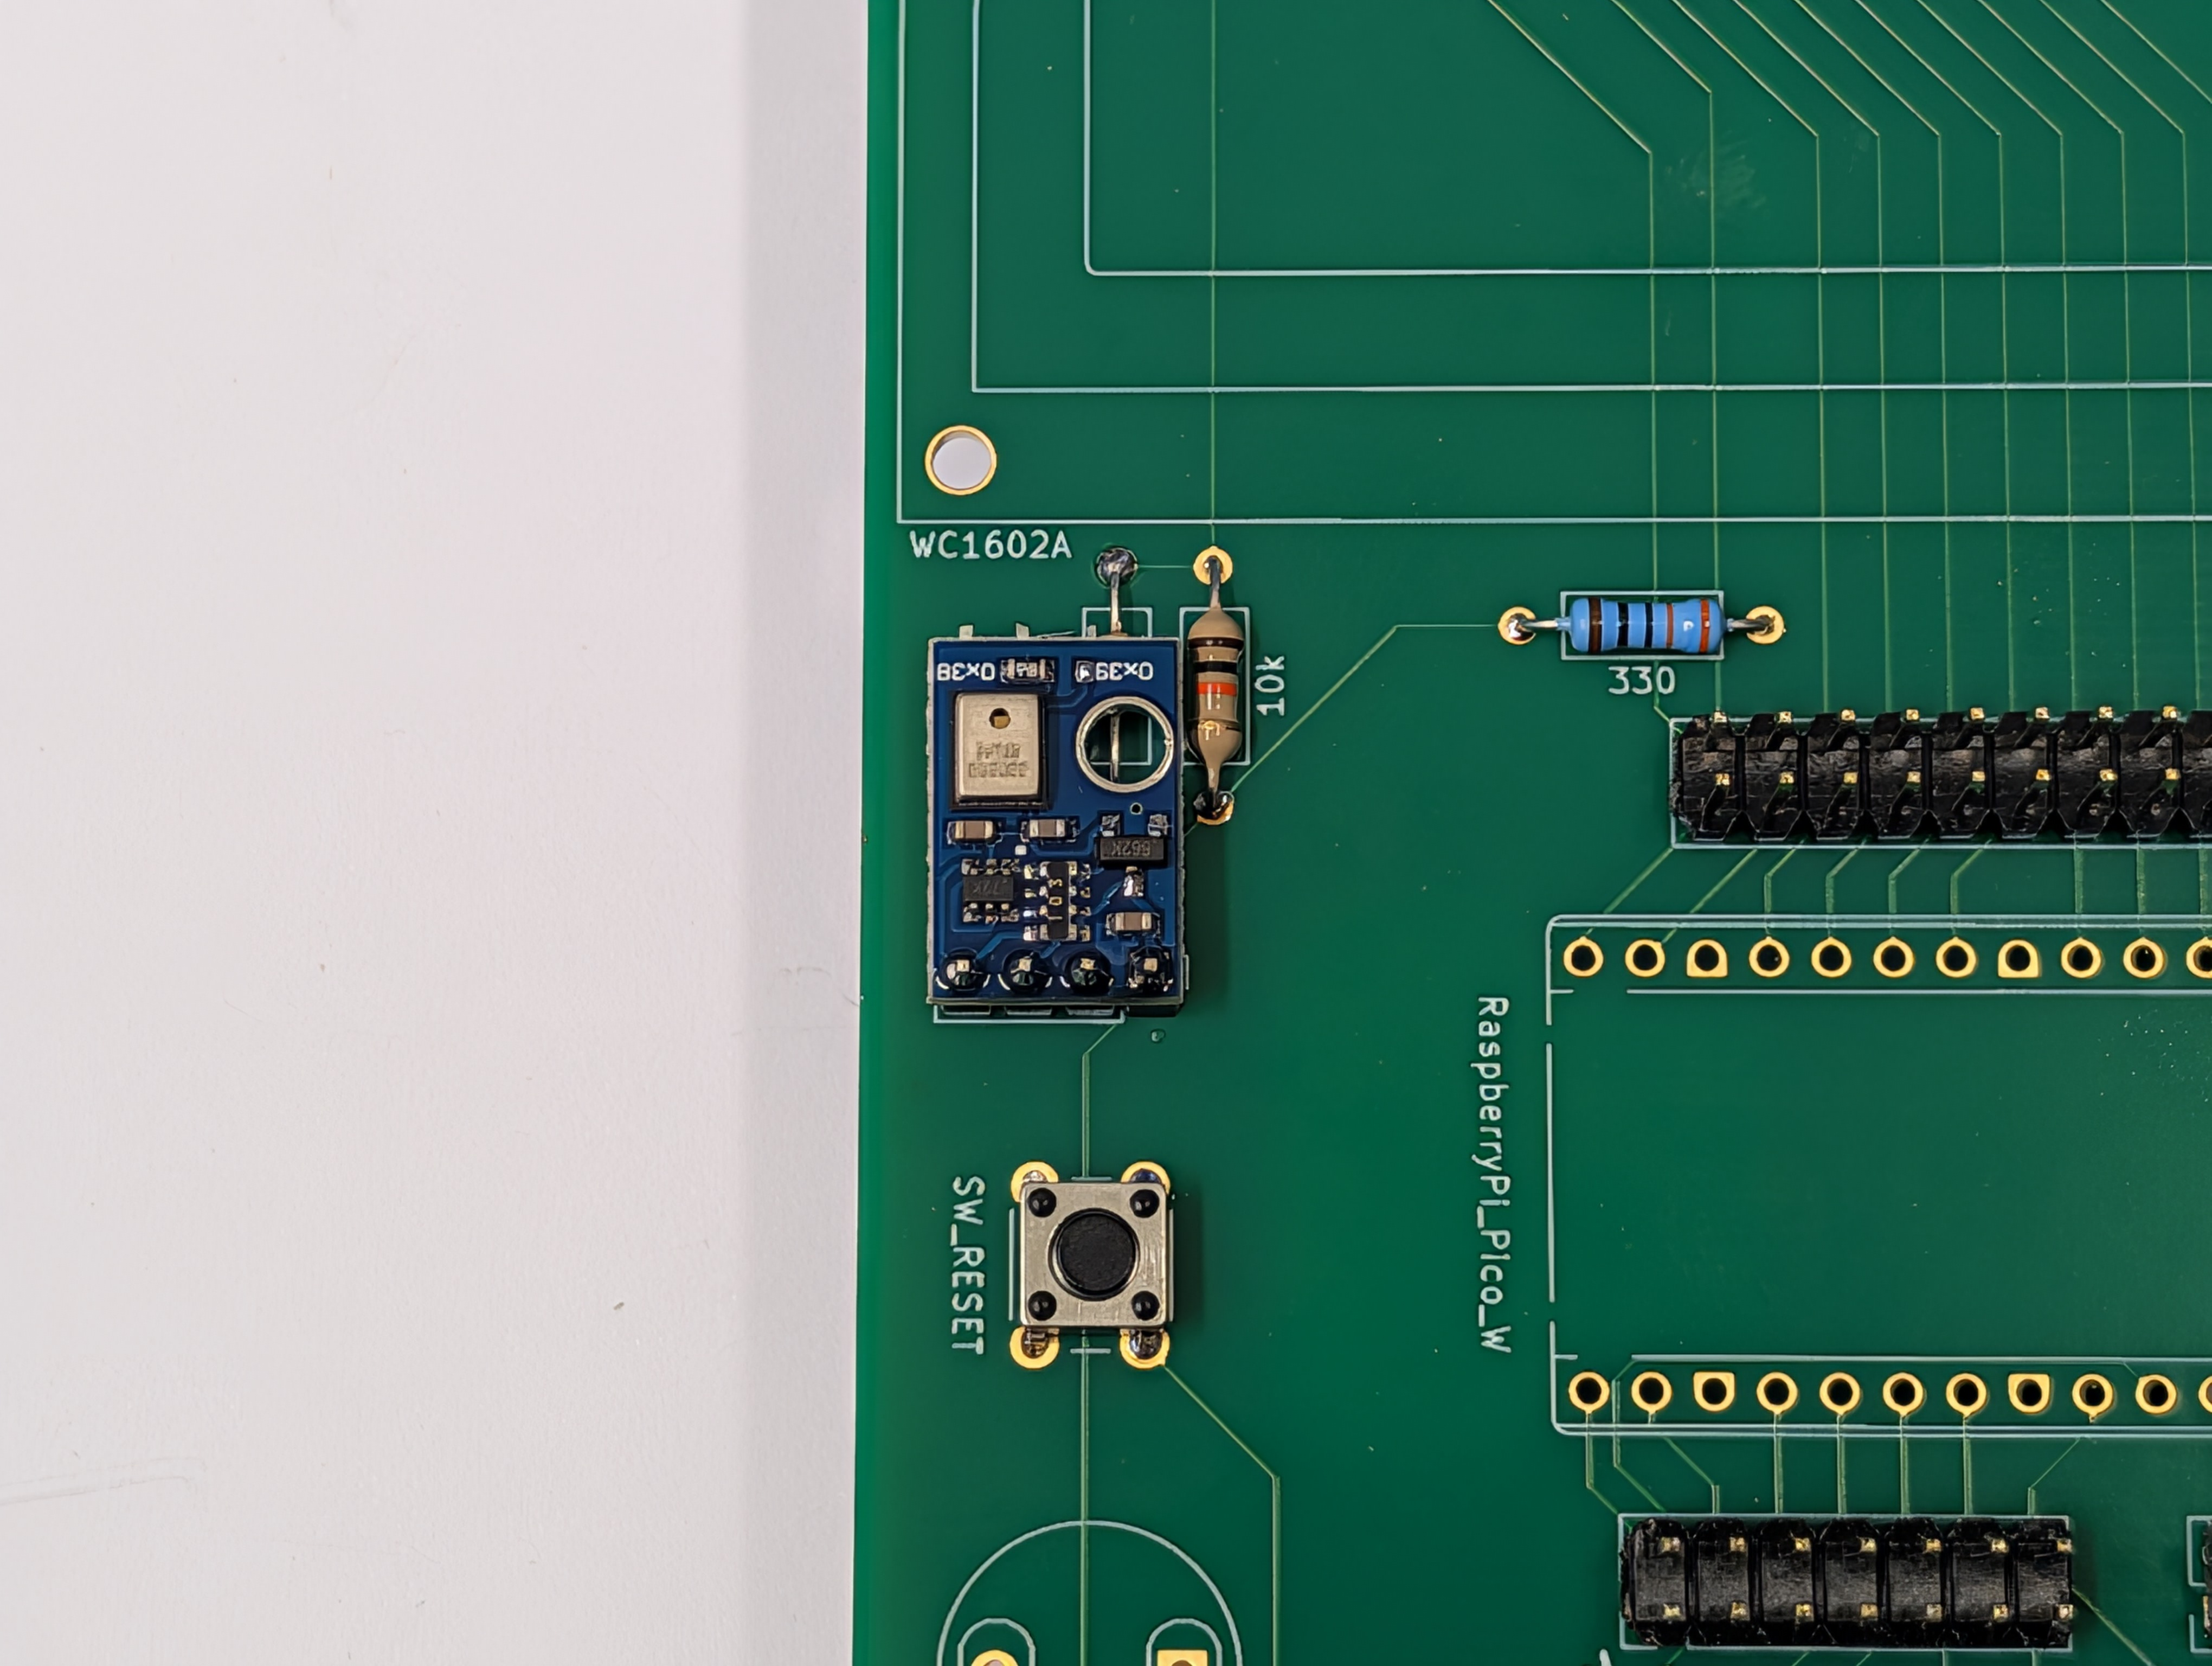
\includegraphics[width=0.75\textwidth]{pictures_of_construction/instruction_step_58.jpg}
\end{figure}

\subsection*{10. Buzzer einbauen}

Jetzt kommt der Buzzer auf die Platine.

\textbf{Wichtig:}
Der Buzzer ist \textbf{gepolt}. Das bedeutet: Er muss richtig herum eingebaut werden.

Achte auf das \textbf{Pluszeichen}:
\begin{itemize}
    \item Auf der Platine ist ein \textbf{+}
    \item Auf dem Buzzer ist auch ein \textbf{+}
\end{itemize}

Diese beiden müssen zusammenpassen.

Merke:
\begin{itemize}
    \item Der \textbf{längere Draht} ist der \textbf{Pluspol}
\end{itemize}

Dann:
\begin{enumerate}
    \item richtig herum einsetzen
    \item festlöten
\end{enumerate}

\begin{figure}[H]
    \centering
    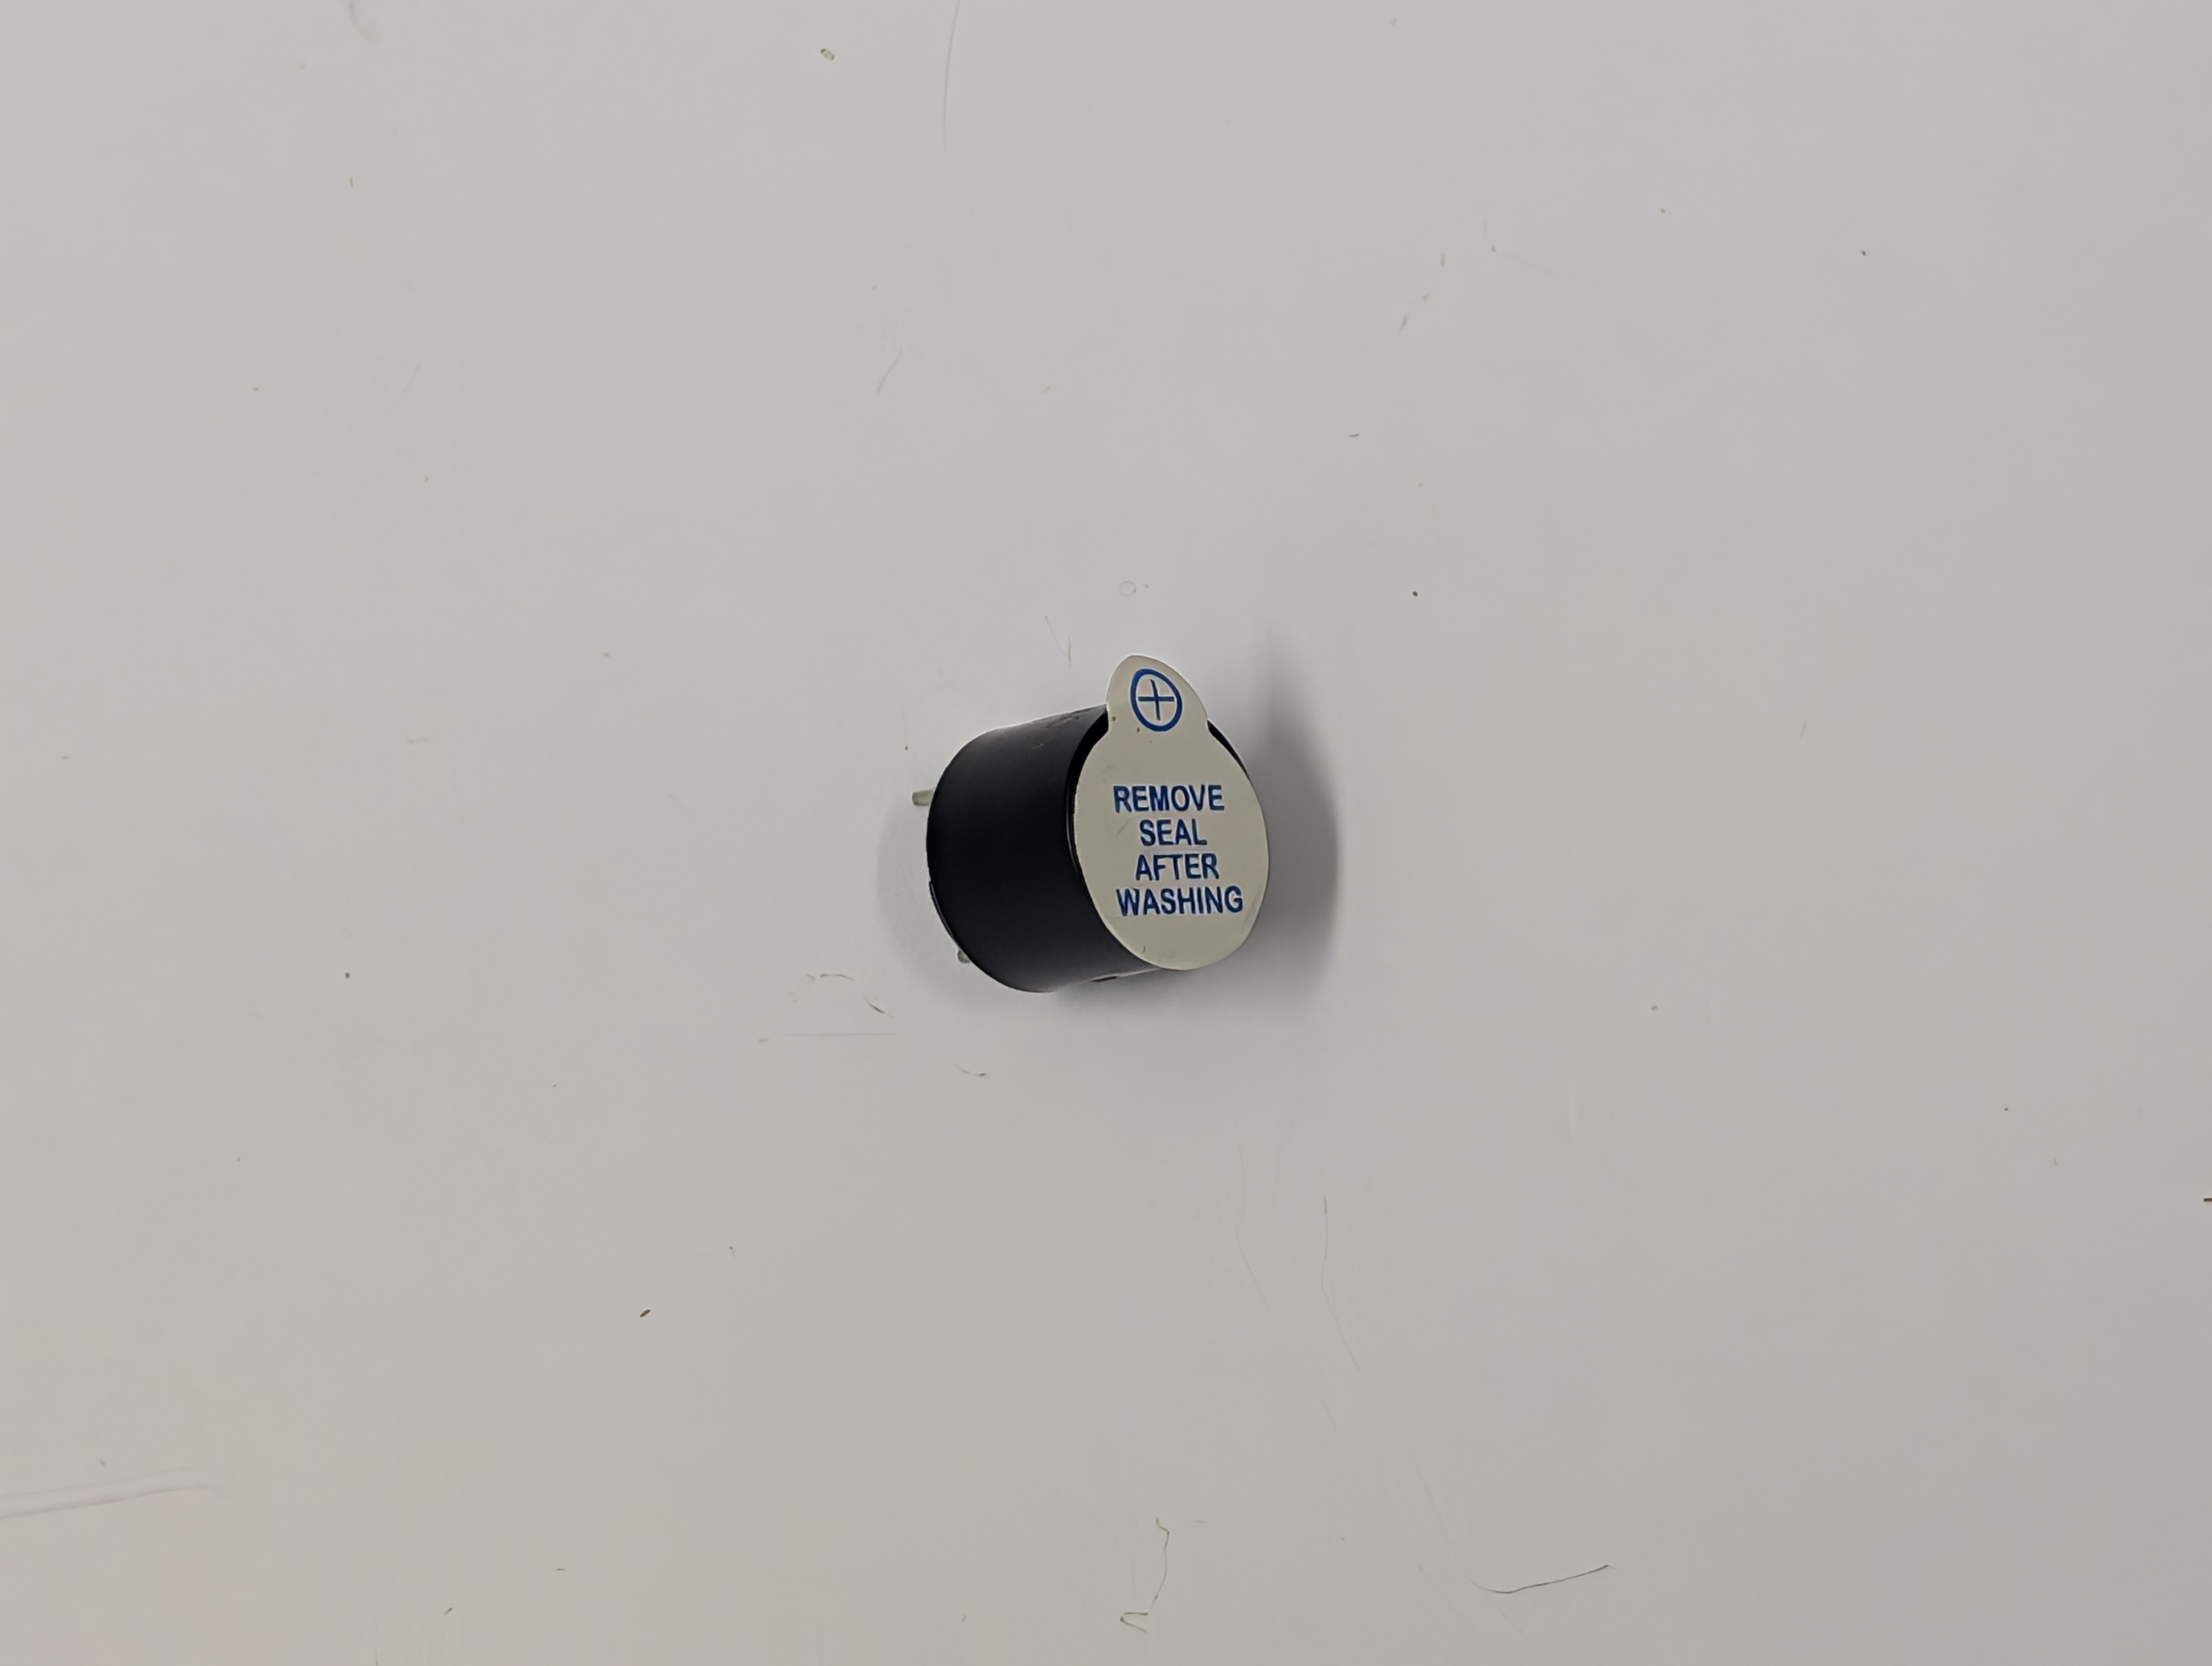
\includegraphics[width=0.75\textwidth]{pictures_of_construction/instruction_step_59.jpg}
\end{figure}

\begin{figure}[H]
    \centering
    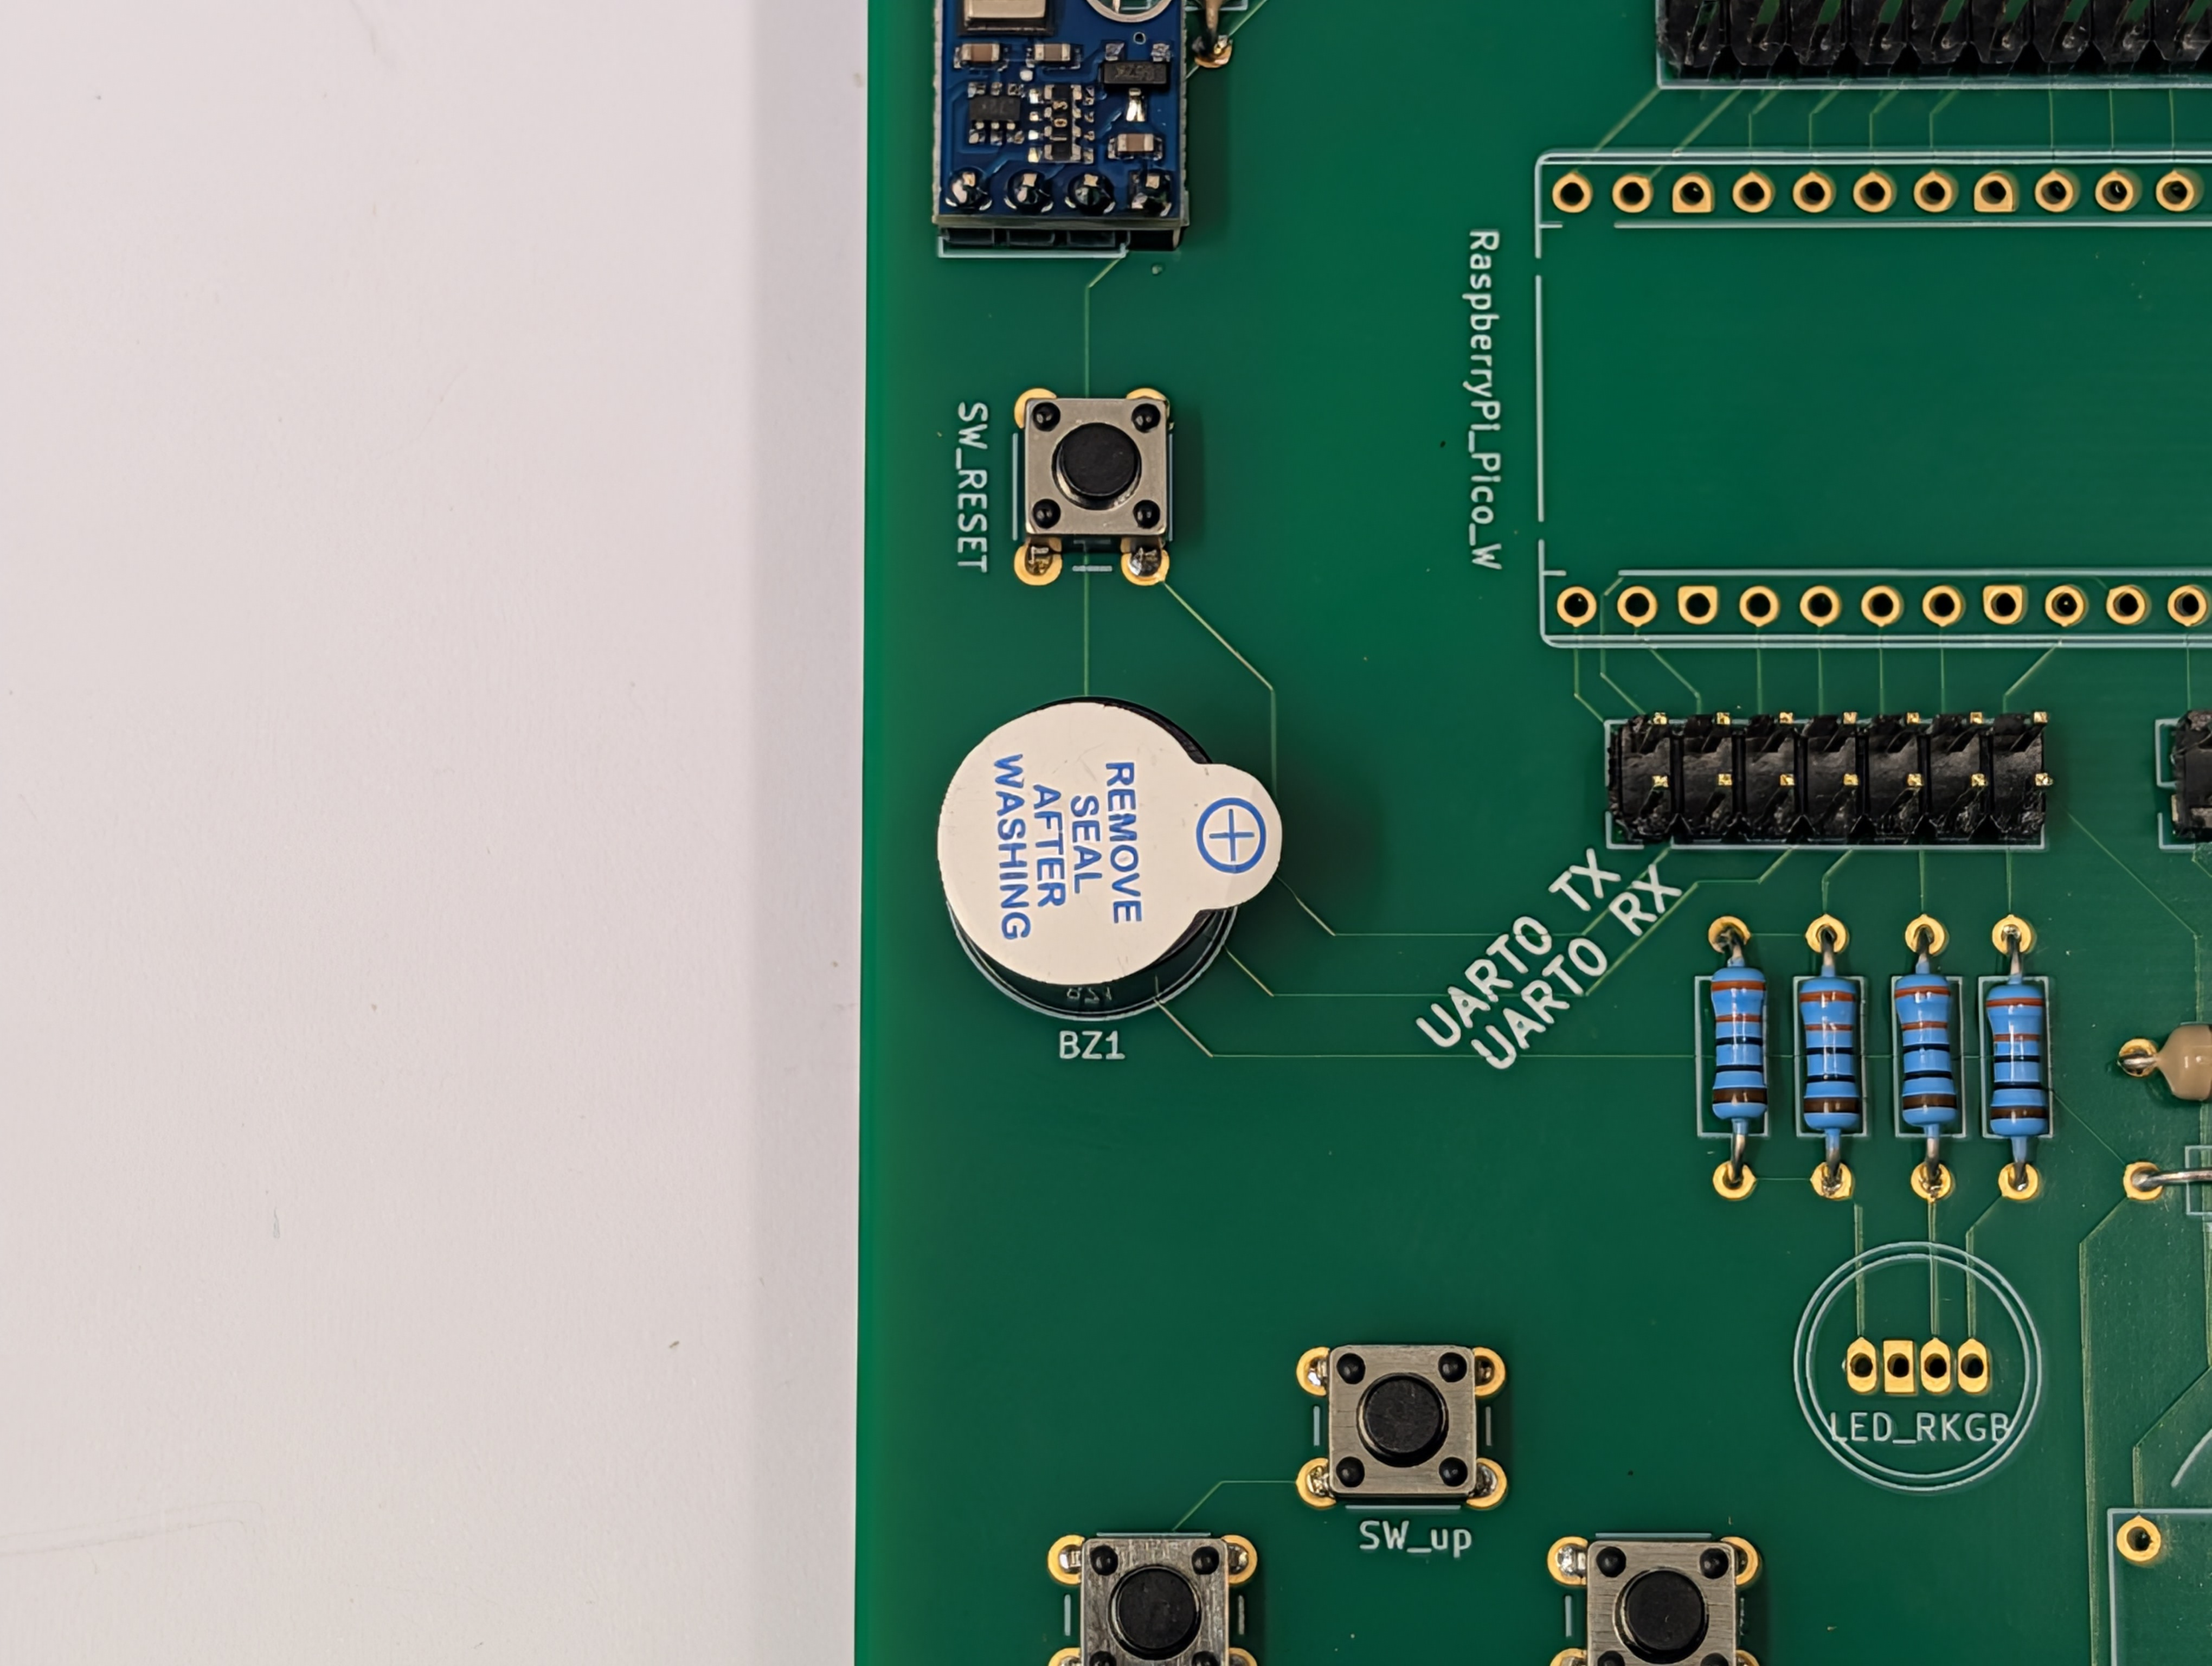
\includegraphics[width=0.75\textwidth]{pictures_of_construction/instruction_step_60.jpg}
\end{figure}

\subsection*{11. LCD-Display einbauen}

Jetzt wird das vorbereitete LCD-Display eingesetzt.

So geht’s:
\begin{enumerate}
    \item In die richtige Position stecken
    \item einen Pin löten
    \item prüfen, ob es gerade sitzt
    \item alle Pins fertig löten
\end{enumerate}

Auch hier gilt:
\begin{itemize}
    \item Für das Kürzen der Pins lieber den größeren Schneider benutzen.
\end{itemize}

\begin{figure}[H]
    \centering
    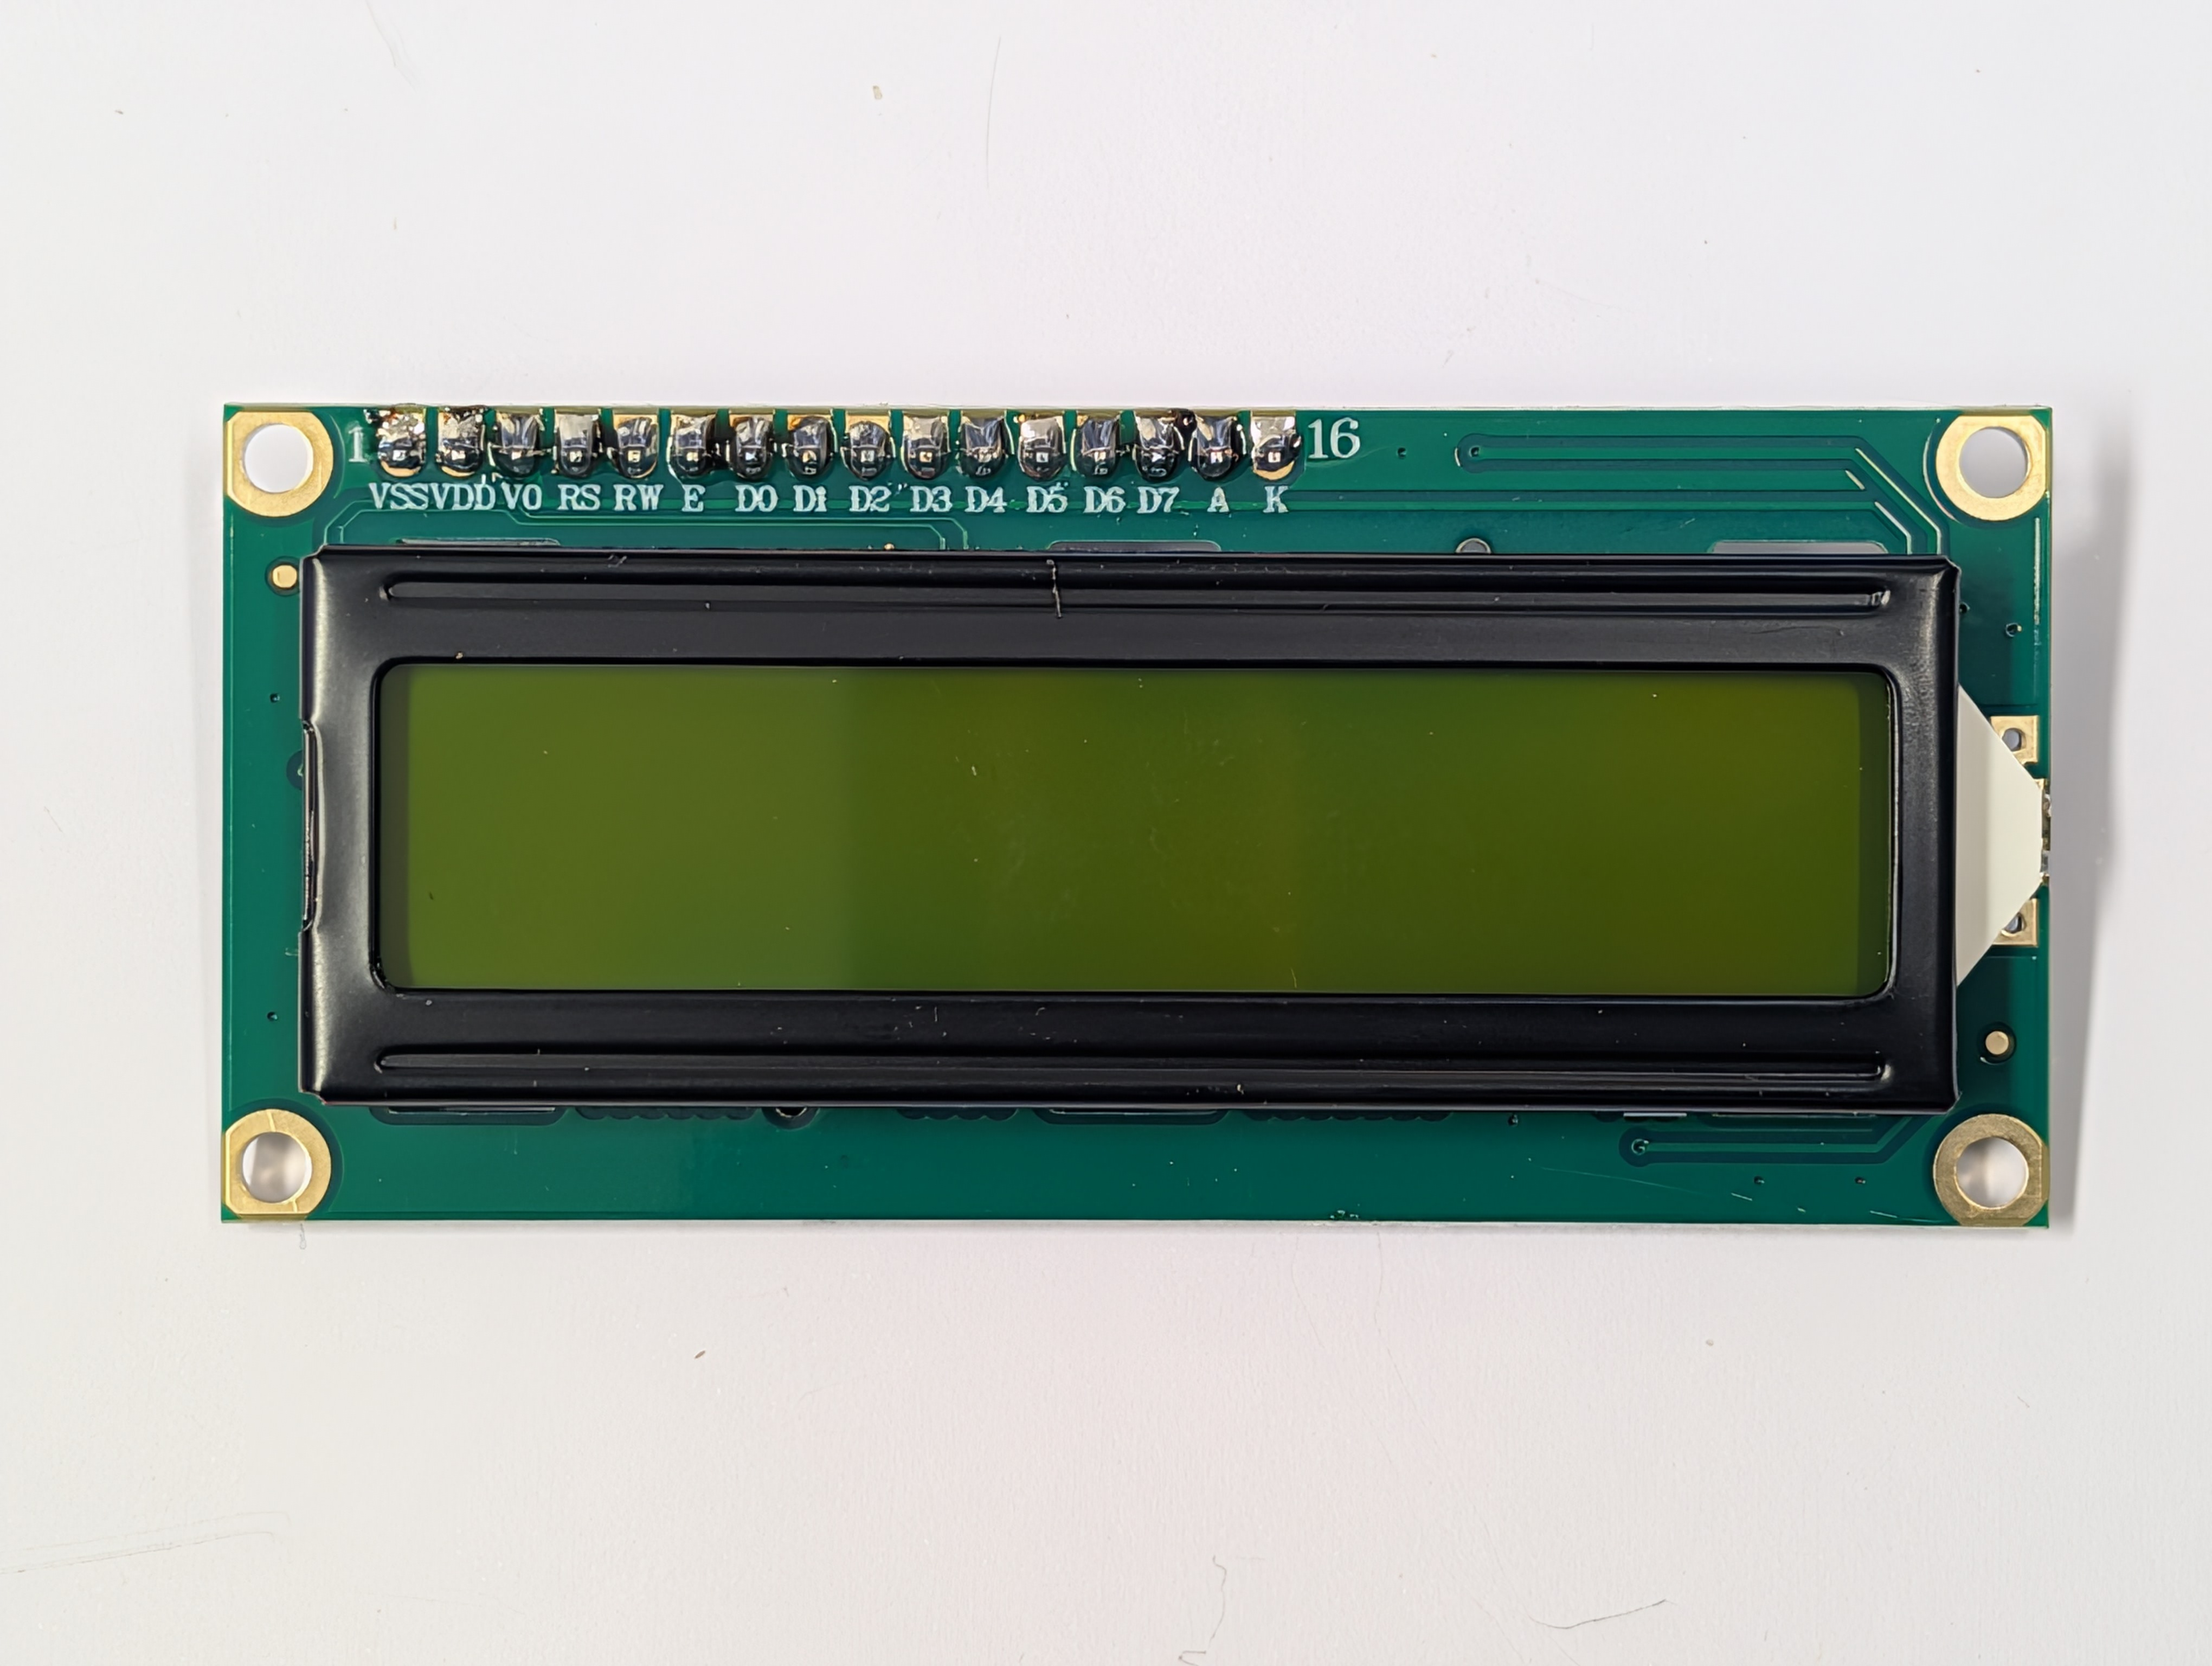
\includegraphics[width=0.75\textwidth]{pictures_of_construction/instruction_step_61.jpg}
\end{figure}

\begin{figure}[H]
    \centering
    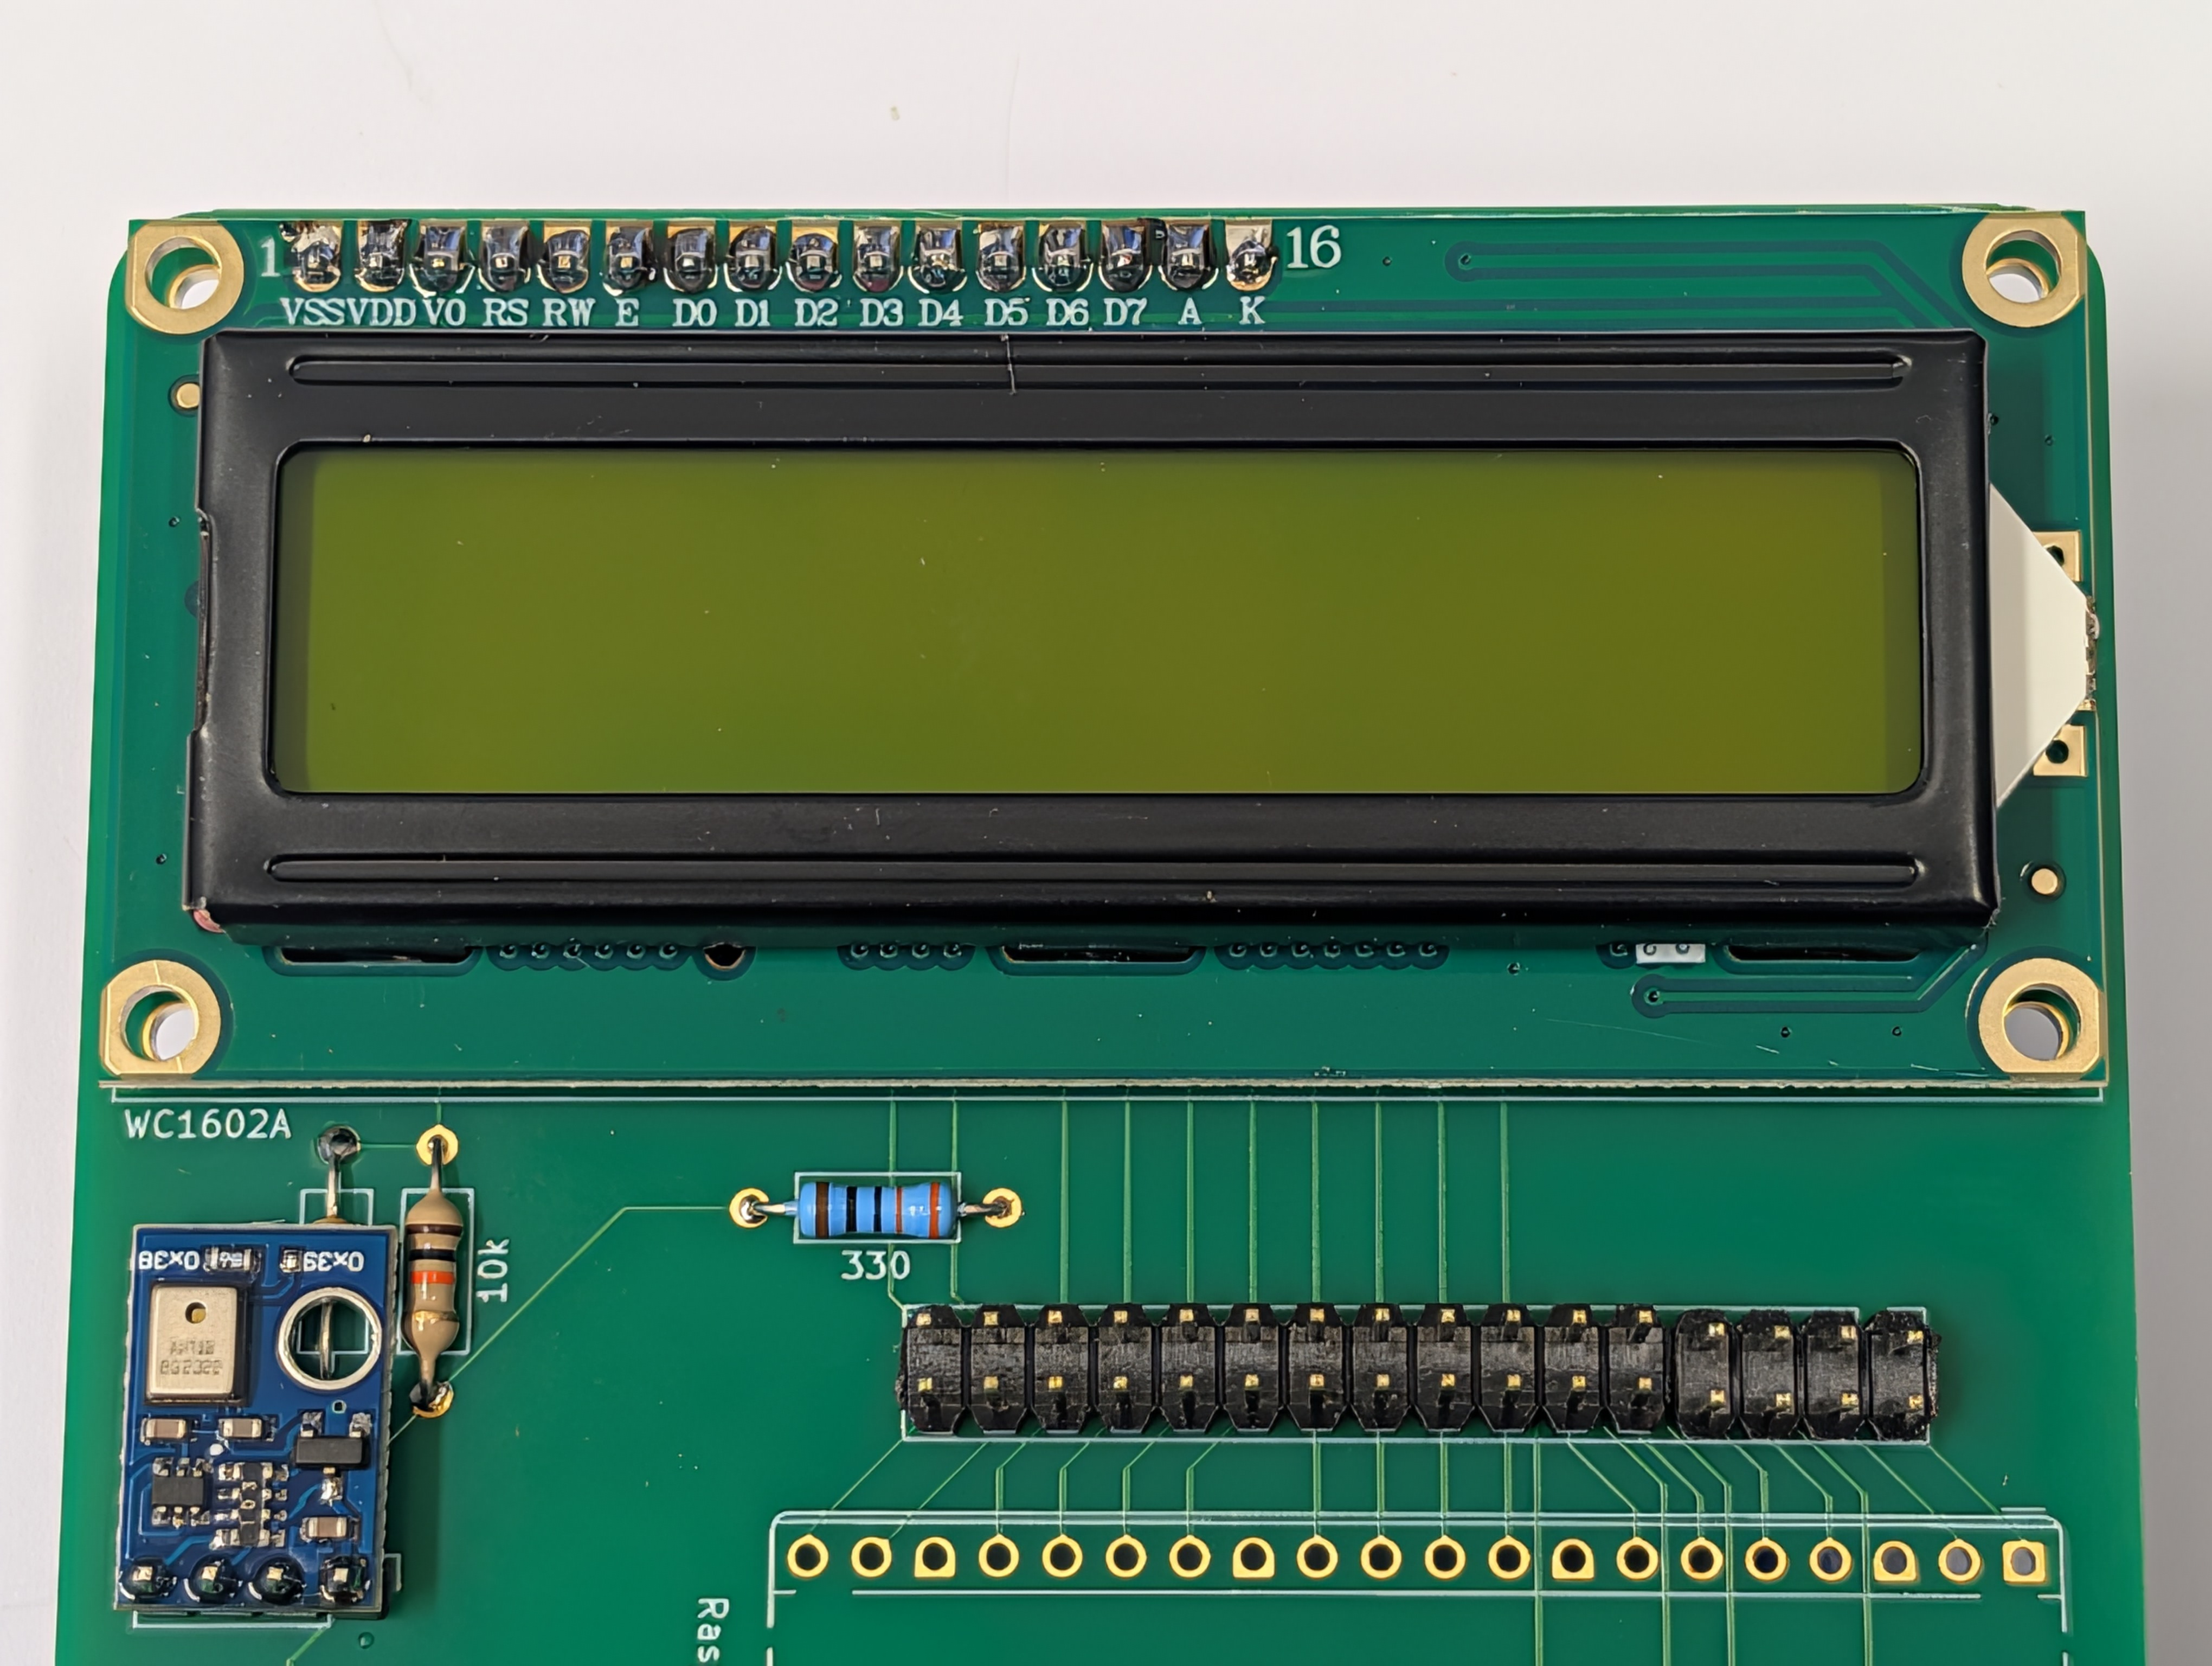
\includegraphics[width=0.75\textwidth]{pictures_of_construction/instruction_step_62.jpg}
\end{figure}

\begin{figure}[H]
    \centering
    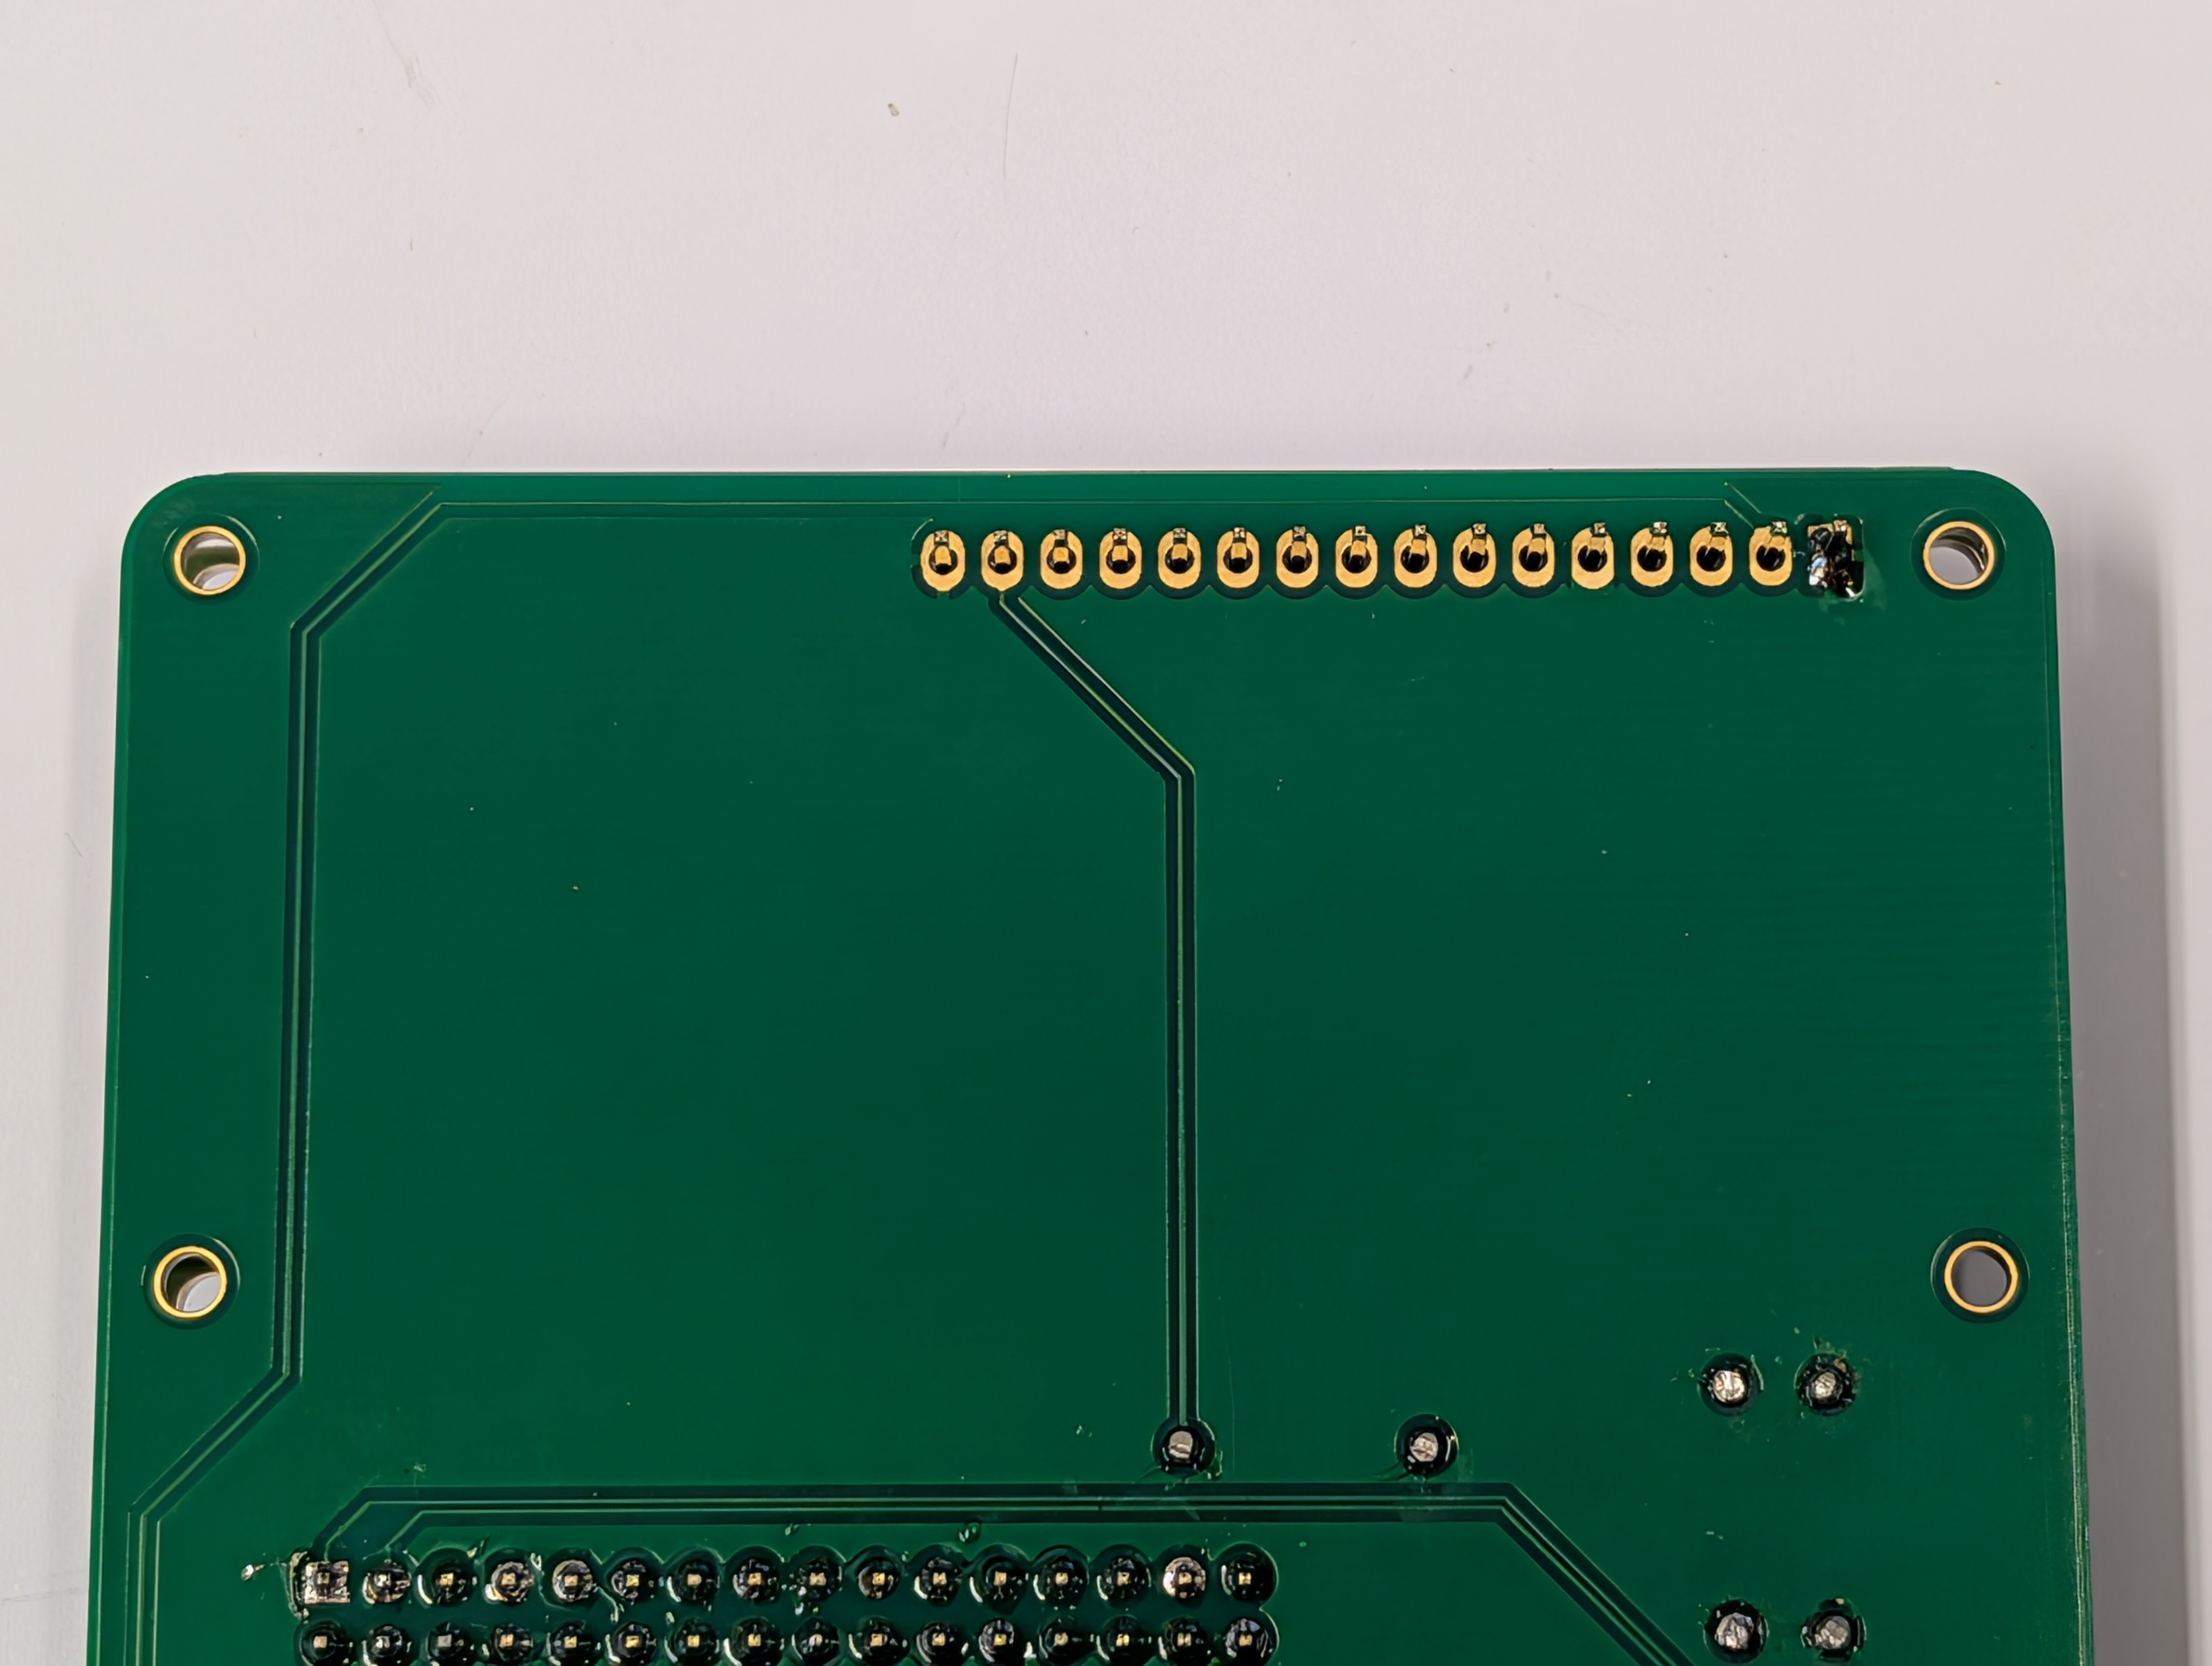
\includegraphics[width=0.75\textwidth]{pictures_of_construction/instruction_step_63.jpg}
\end{figure}

\begin{figure}[H]
    \centering
    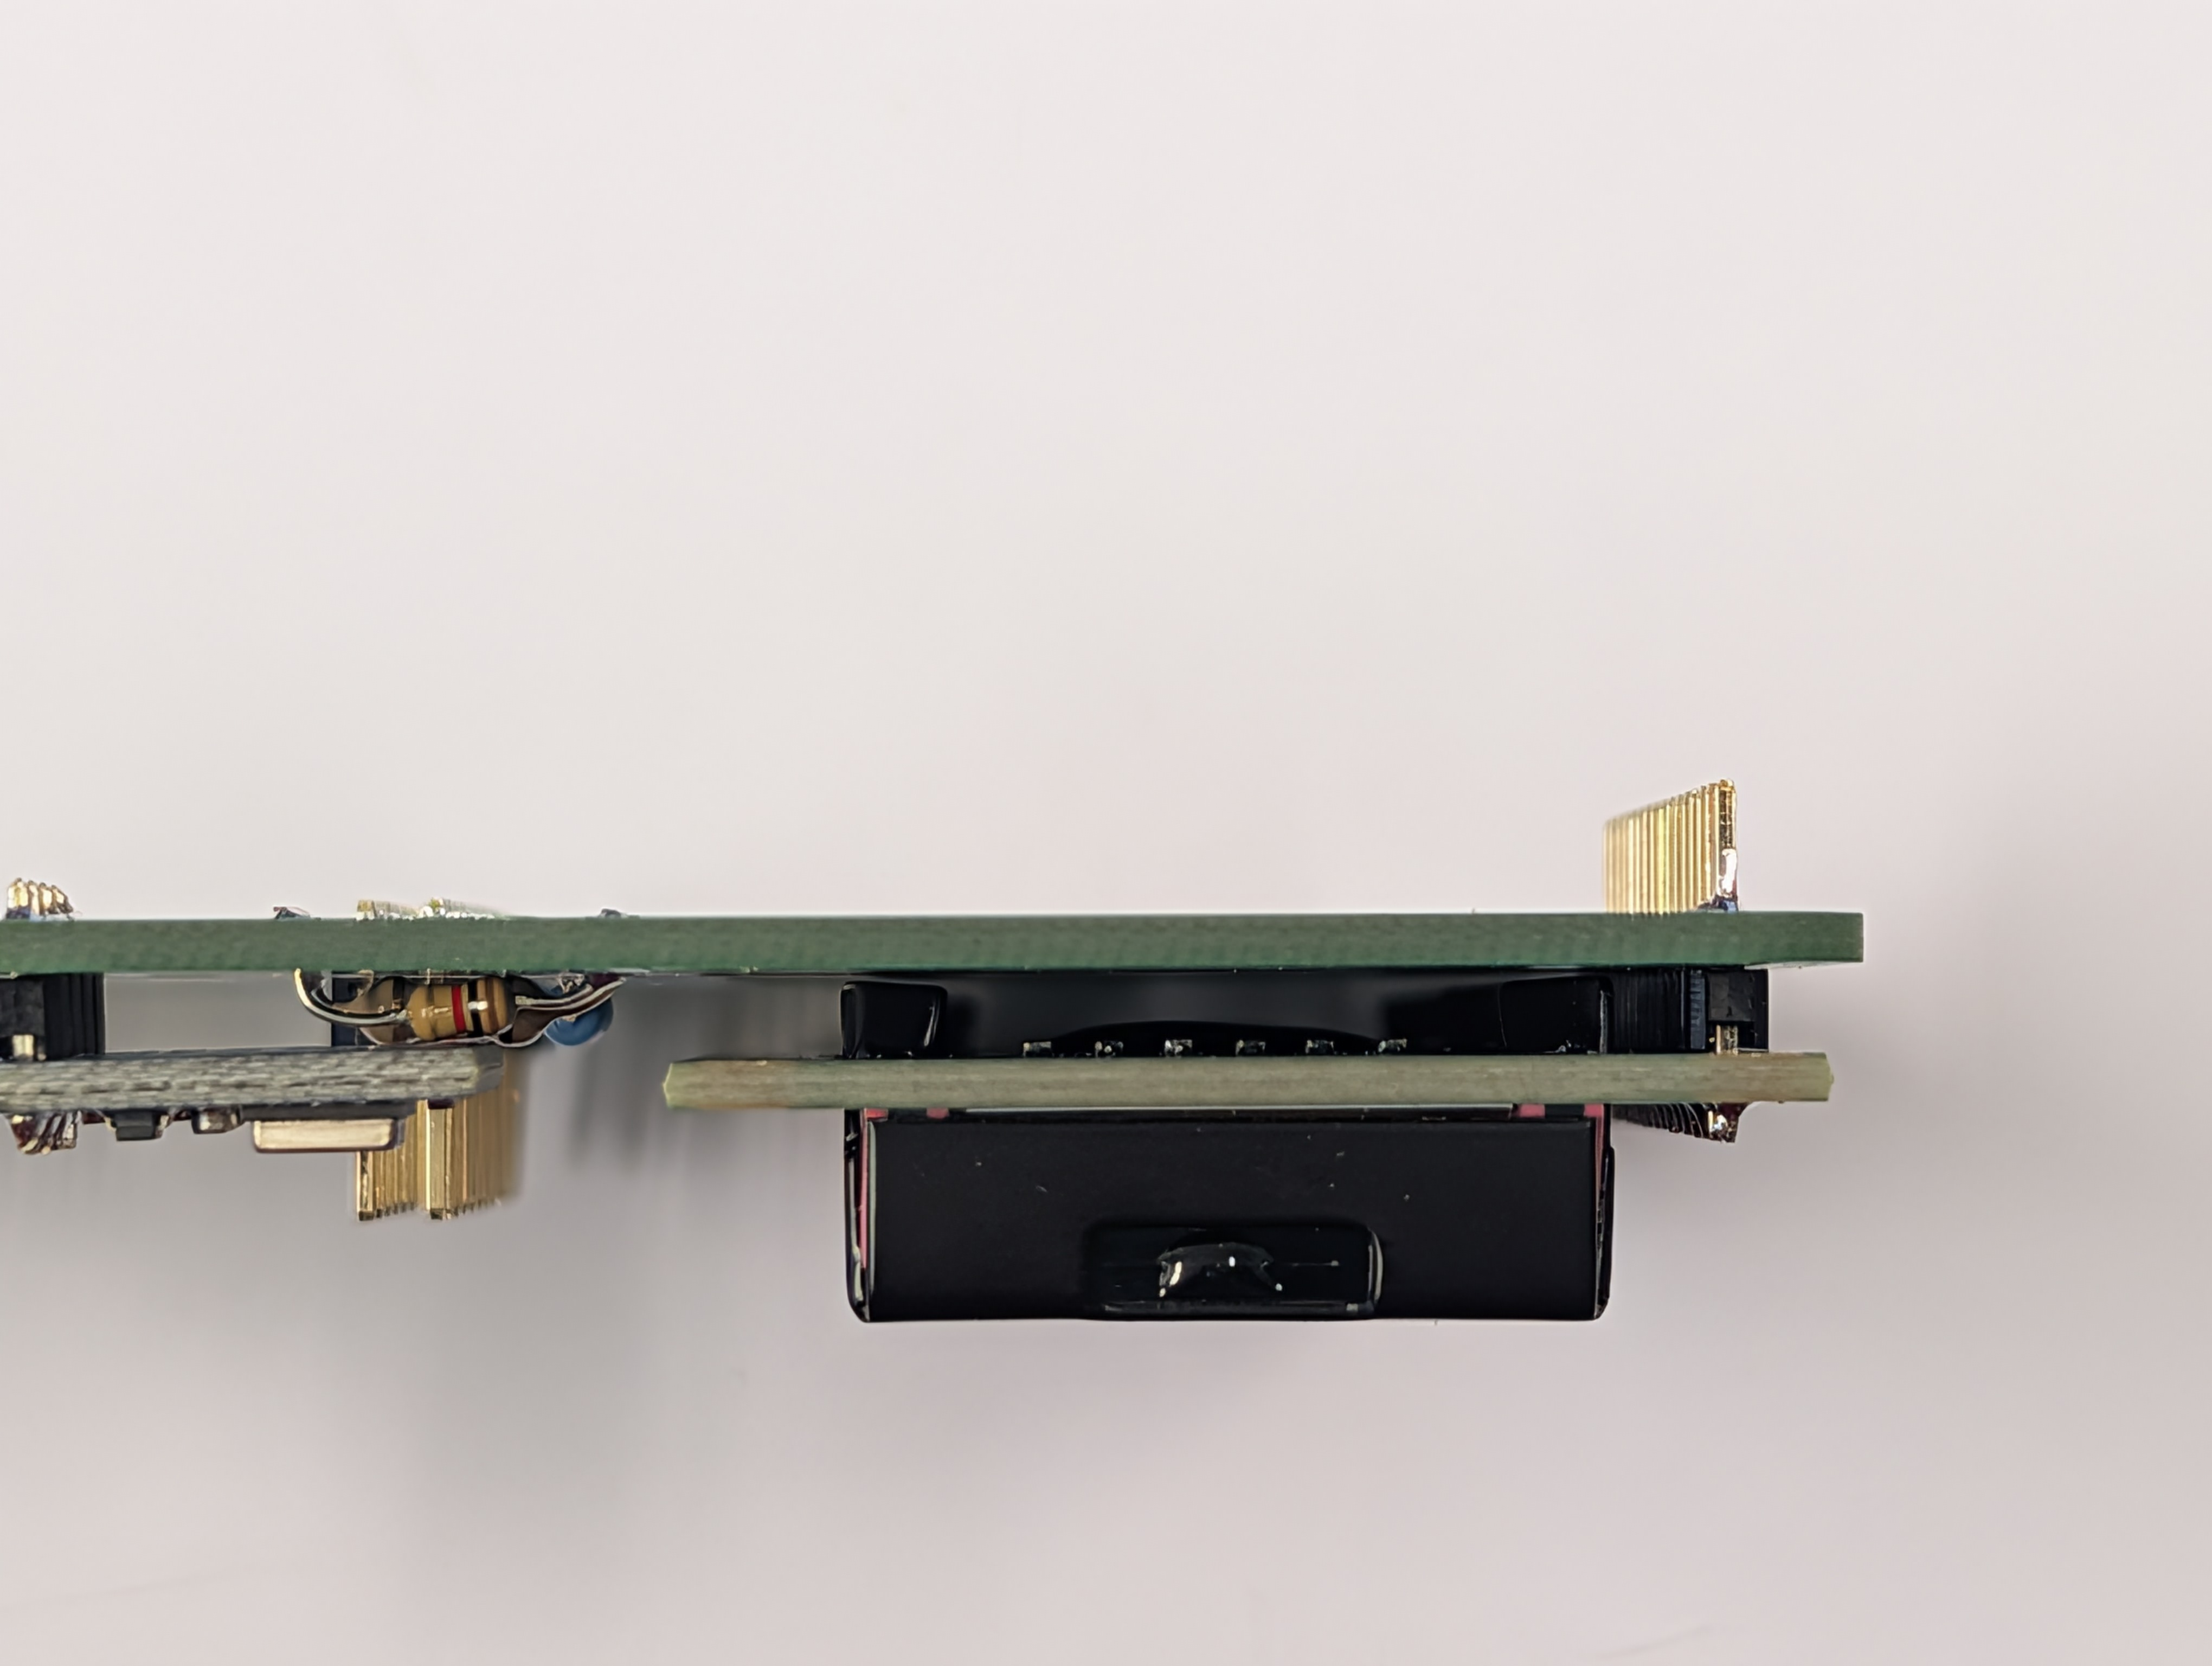
\includegraphics[width=0.75\textwidth]{pictures_of_construction/instruction_step_64.jpg}
\end{figure}

\subsection*{12. RGB-LED einbauen}

Jetzt kommt die bunte LED.

Auch sie muss richtig herum eingebaut werden.

\textbf{Wichtig:}
\begin{itemize}
    \item Die LED ist \textbf{gepolt}
    \item Hier ist das \textbf{längste Bein der Minuspol}
    \item Auf der Platine zeigt ein \textbf{quadratisches Lötpad} den Minuspol
\end{itemize}

So geht’s:
\begin{enumerate}
    \item LED richtig herum einsetzen
    \item festlöten
    \item Drähte abschneiden
\end{enumerate}

Falls die Lötstelle nicht schön aussieht:
\begin{itemize}
    \item mit dem Lötkolben vorsichtig nochmal erwärmen
\end{itemize}

Aber ganz wichtig:
\begin{itemize}
    \item Prüfe danach, ob keine zwei Pins aus Versehen mit Lötzinn verbunden sind.
\end{itemize}

\begin{figure}[H]
    \centering
    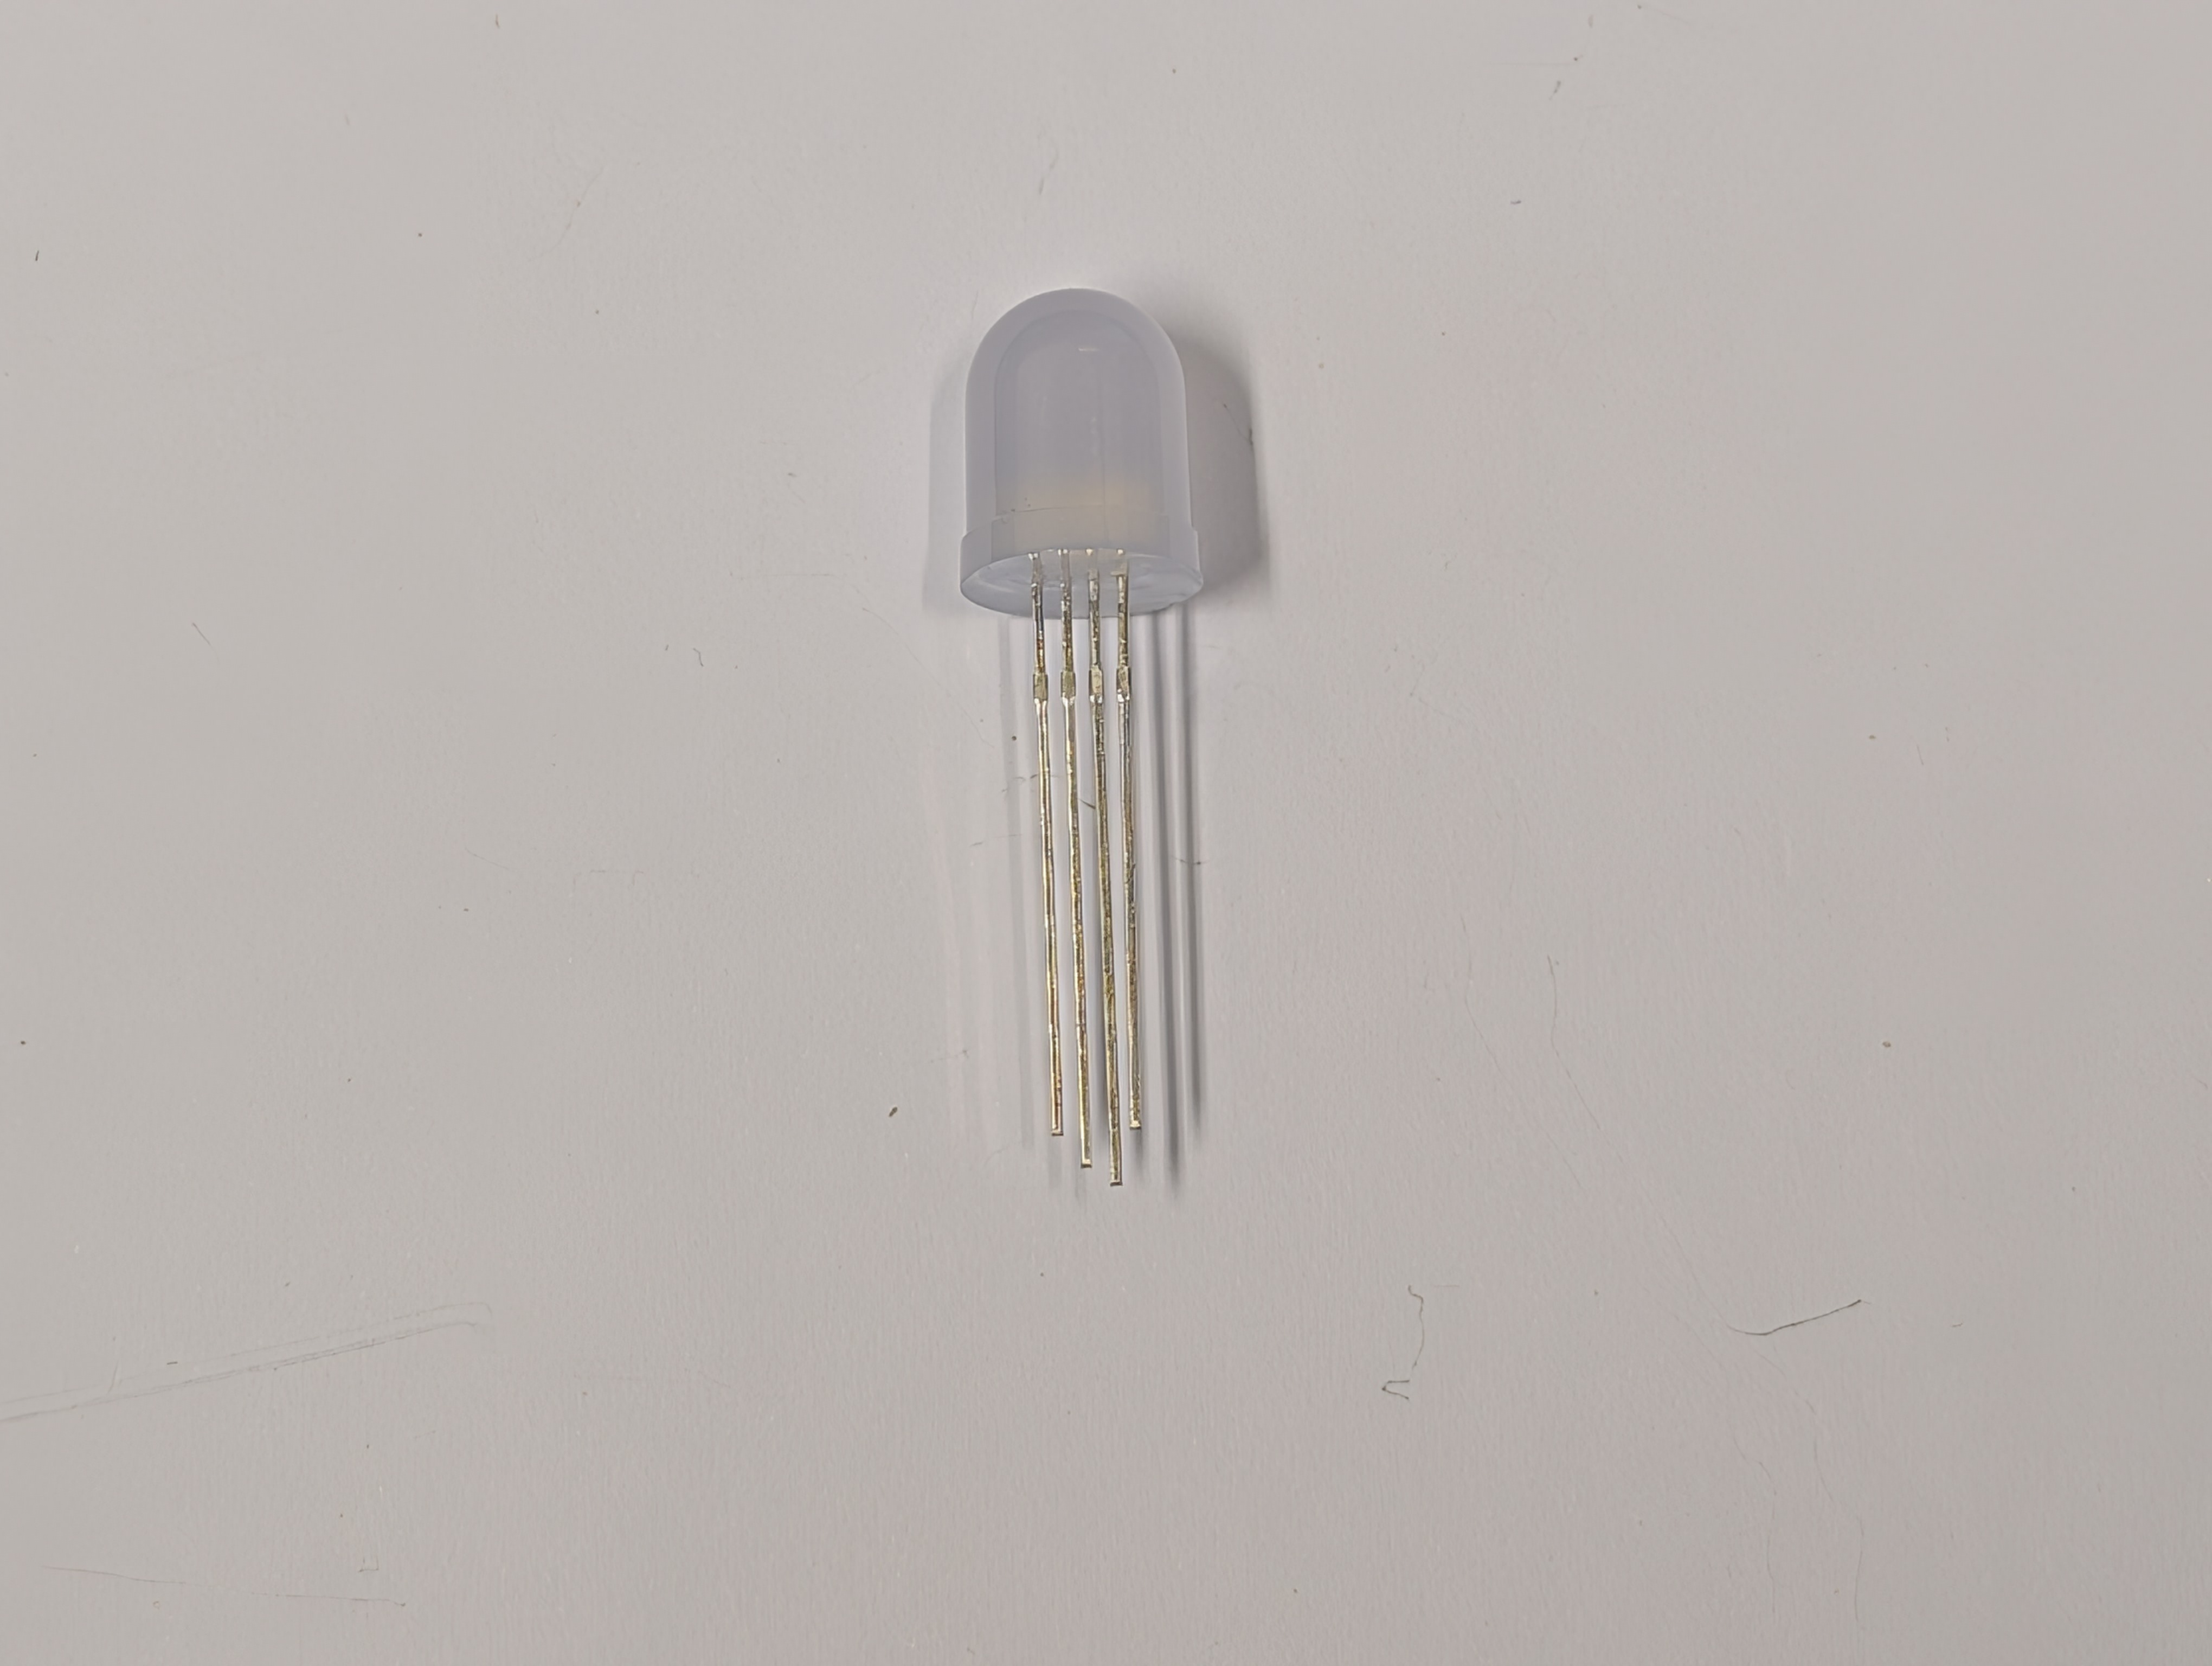
\includegraphics[width=0.75\textwidth]{pictures_of_construction/instruction_step_65.jpg}
\end{figure}

\begin{figure}[H]
    \centering
    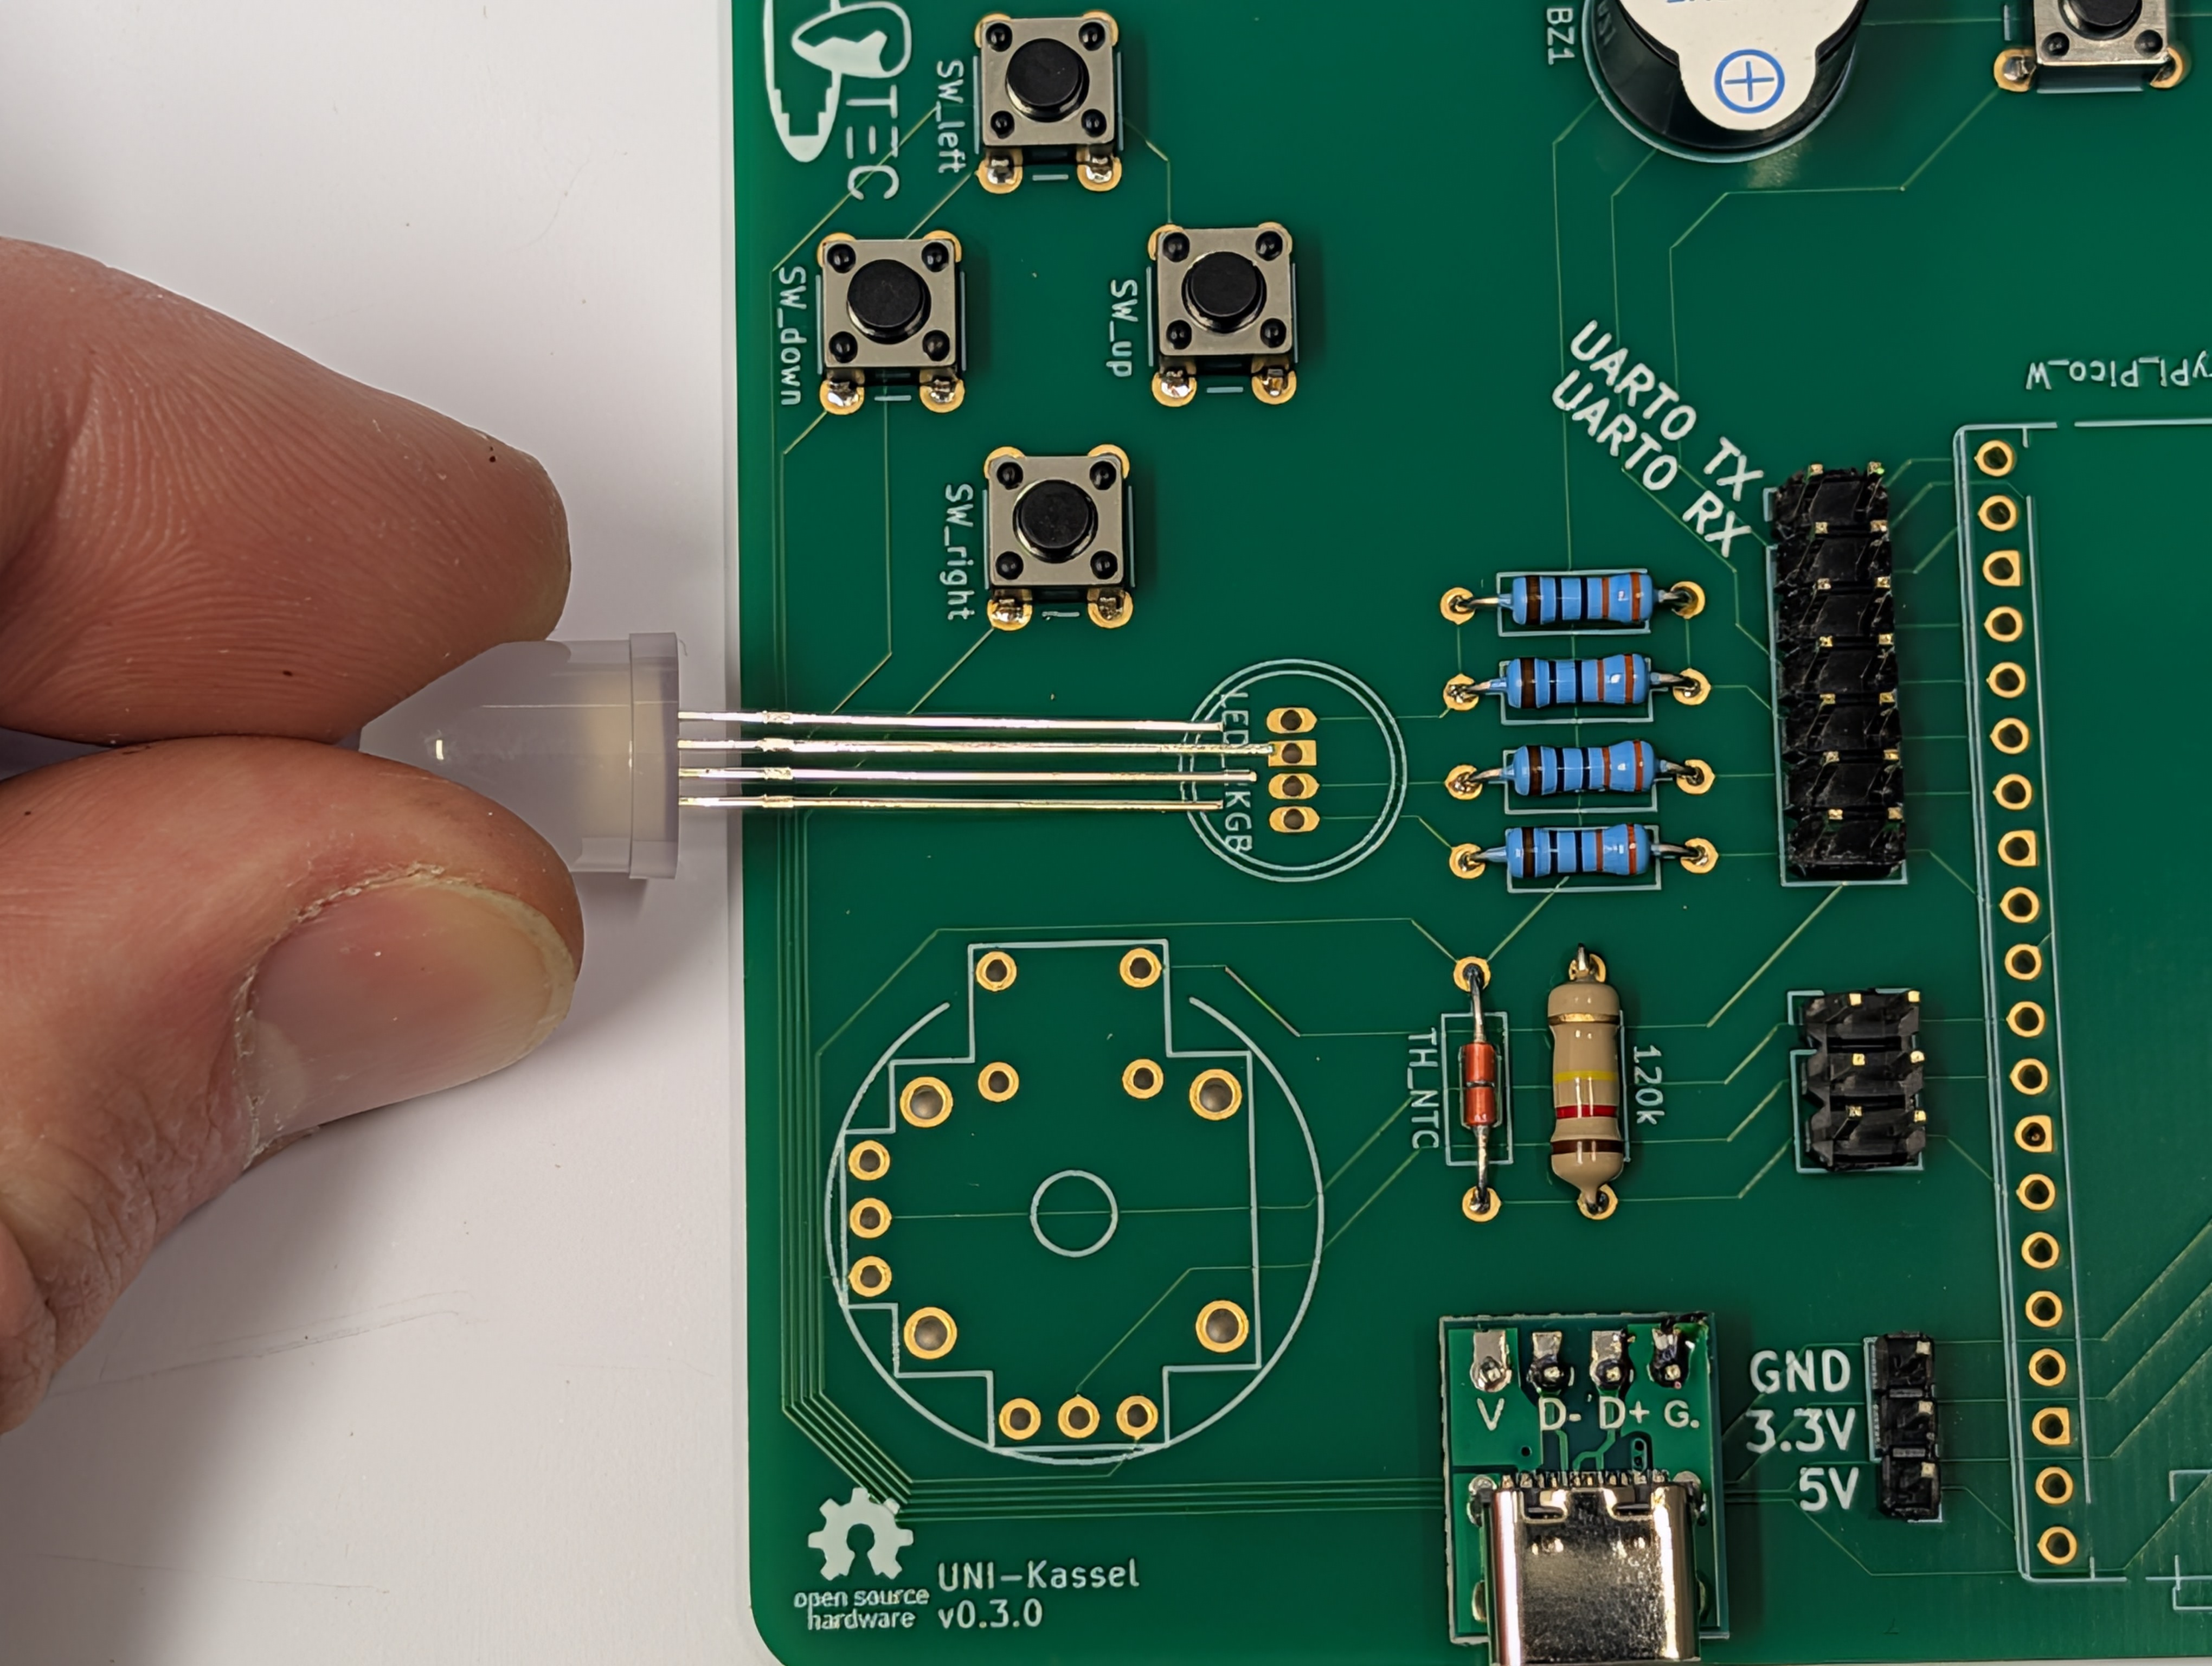
\includegraphics[width=0.75\textwidth]{pictures_of_construction/instruction_step_66.jpg}
\end{figure}

\begin{figure}[H]
    \centering
    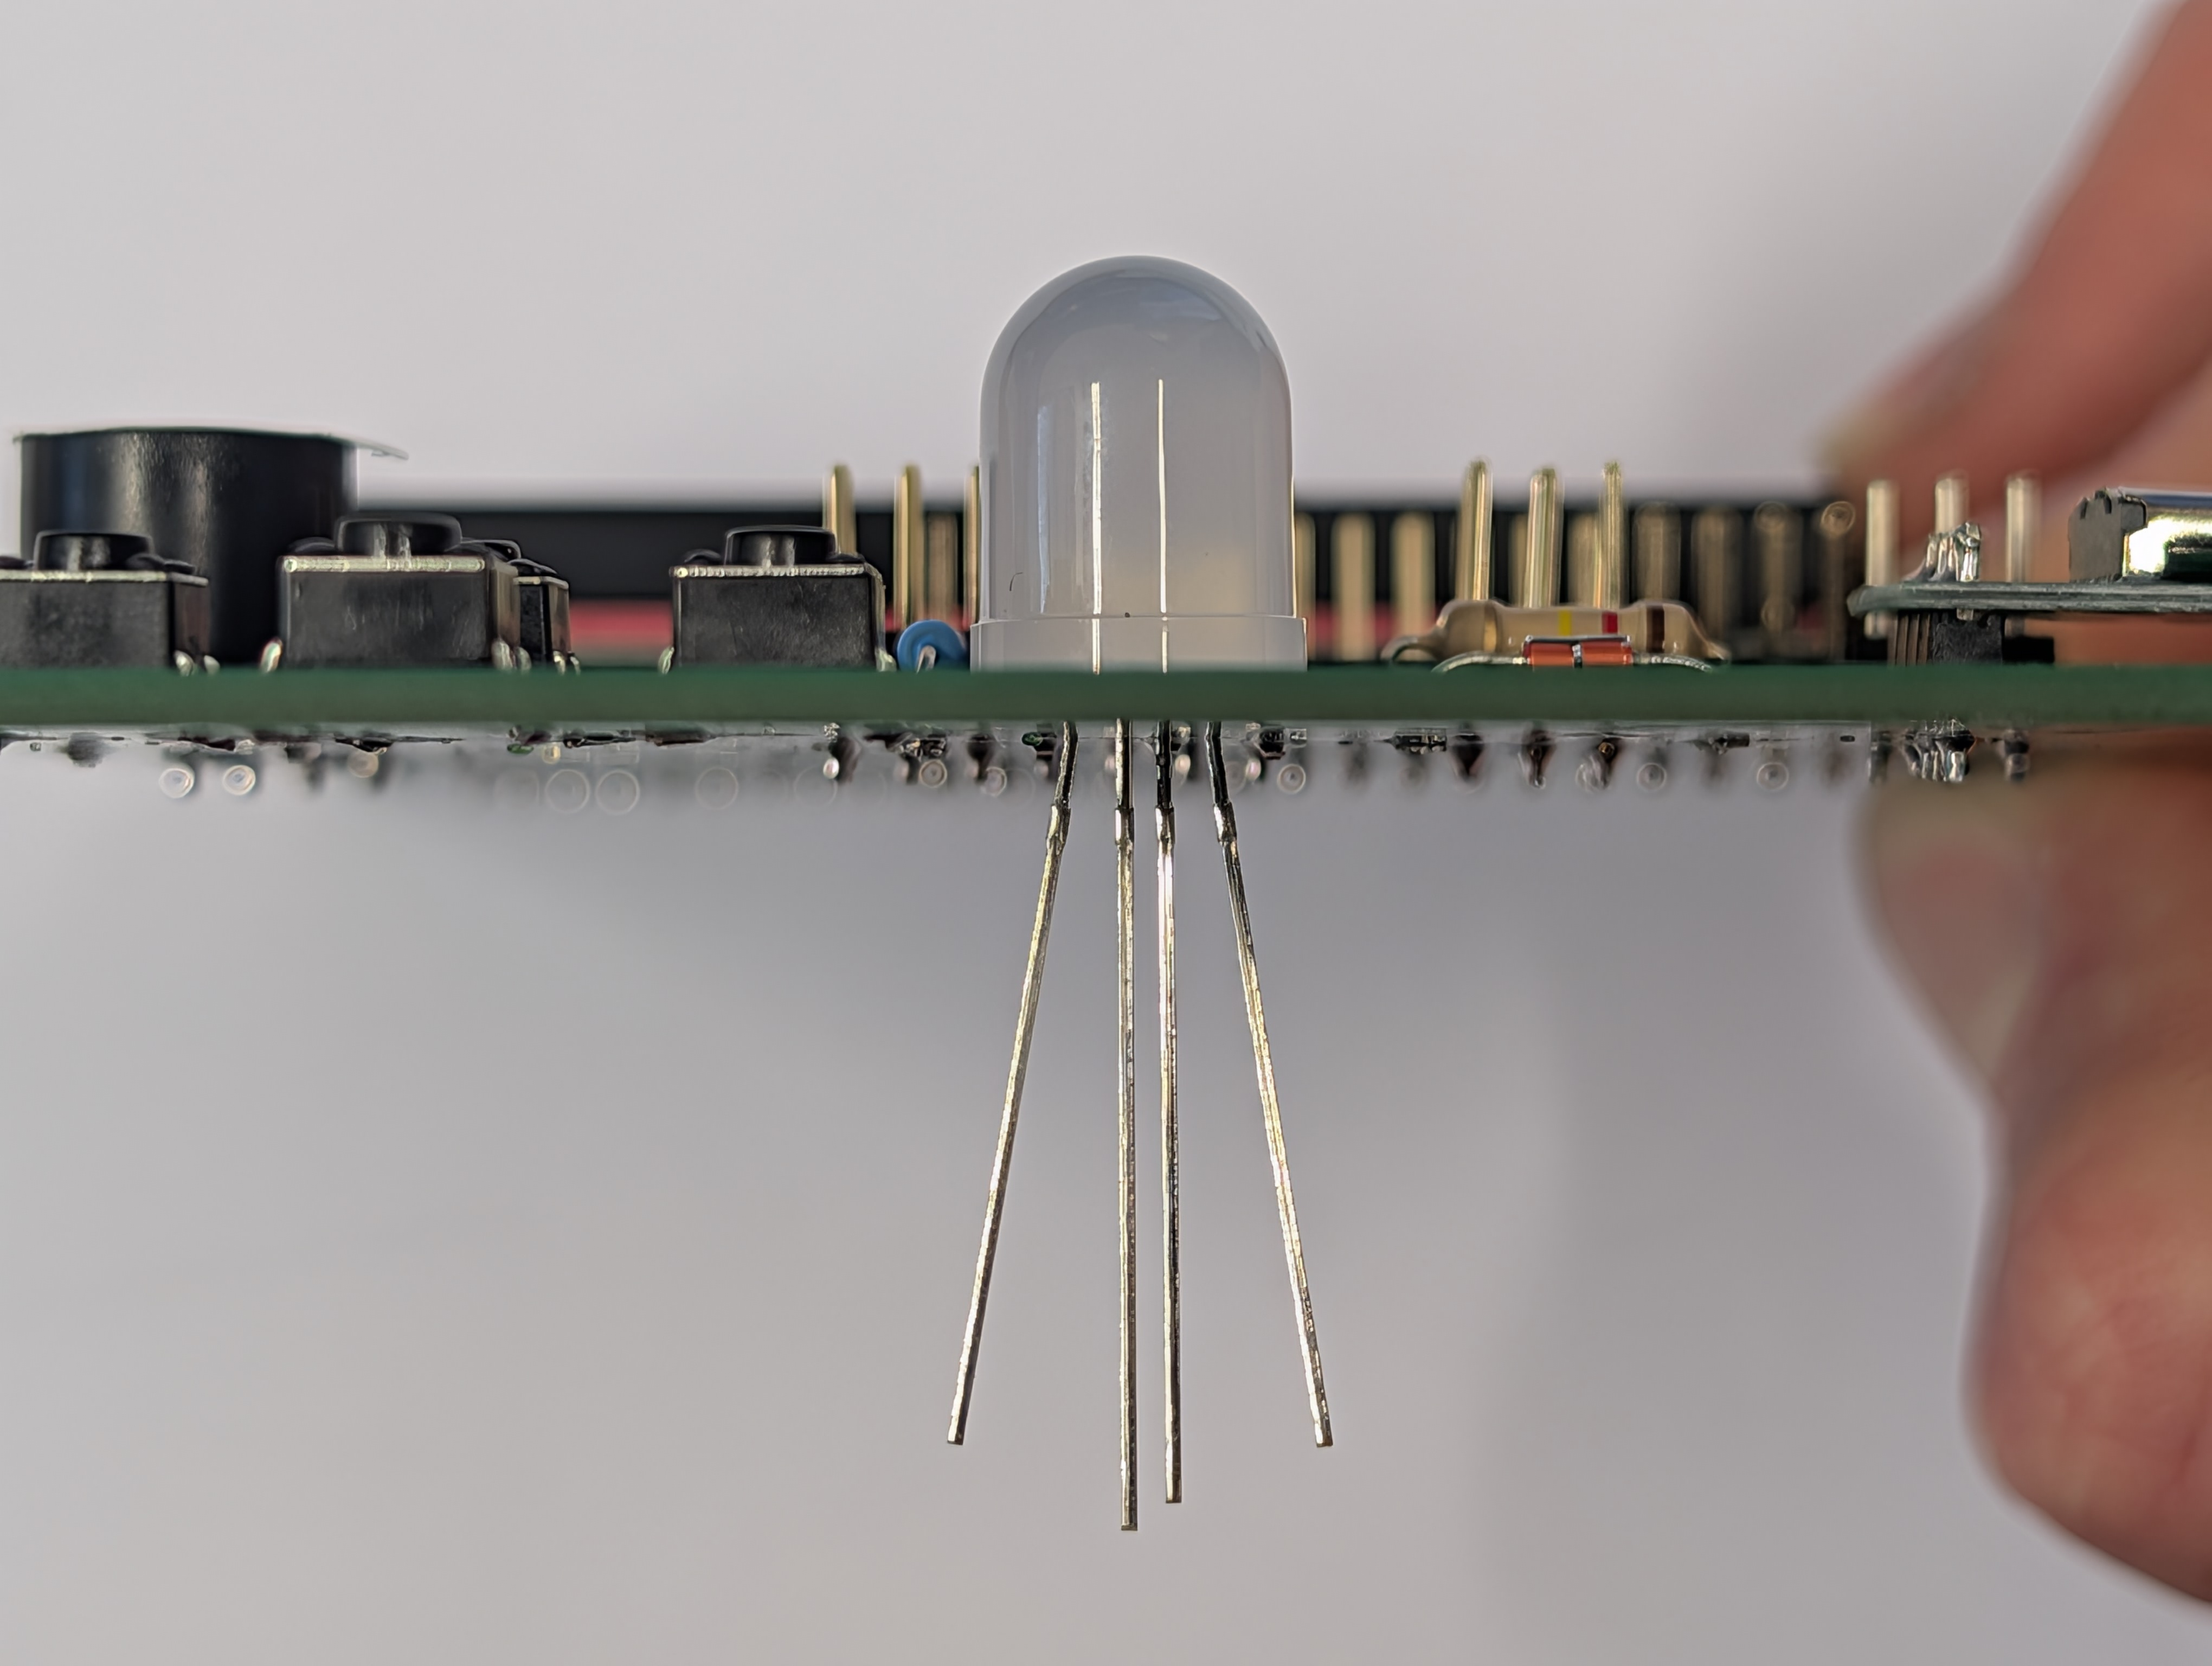
\includegraphics[width=0.75\textwidth]{pictures_of_construction/instruction_step_67.jpg}
\end{figure}

\begin{figure}[H]
    \centering
    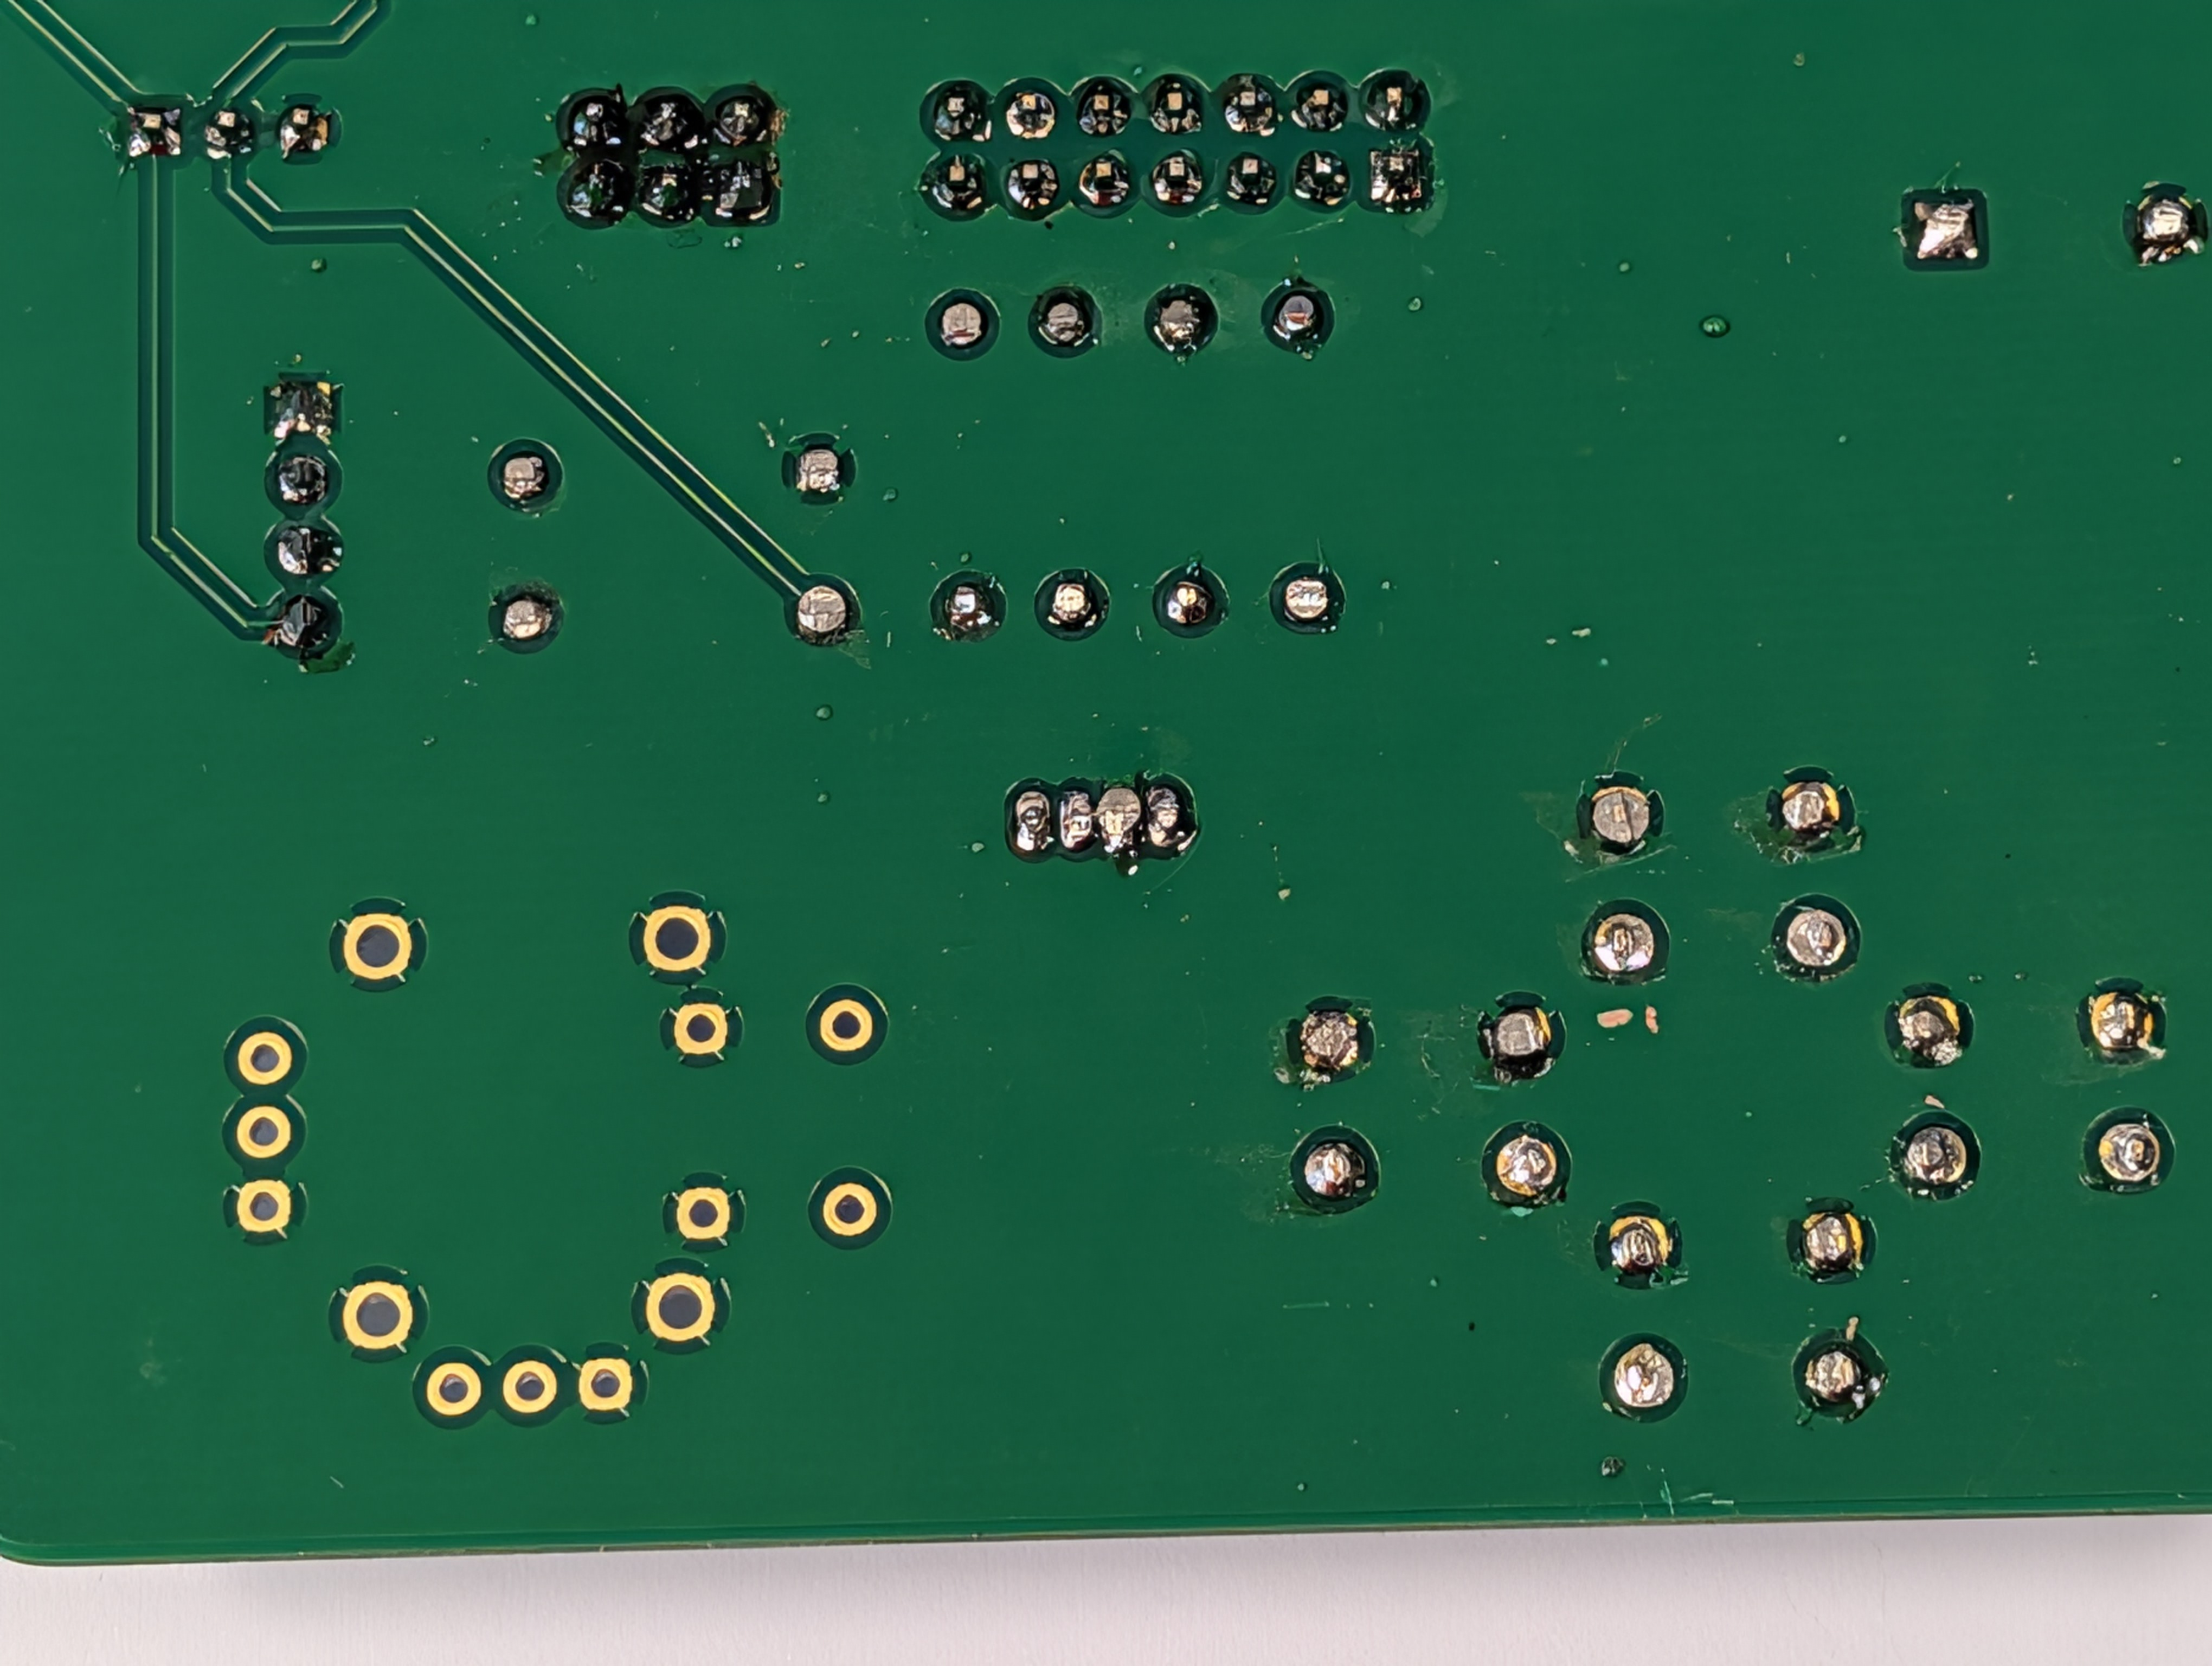
\includegraphics[width=0.75\textwidth]{pictures_of_construction/instruction_step_68.jpg}
\end{figure}

\begin{figure}[H]
    \centering
    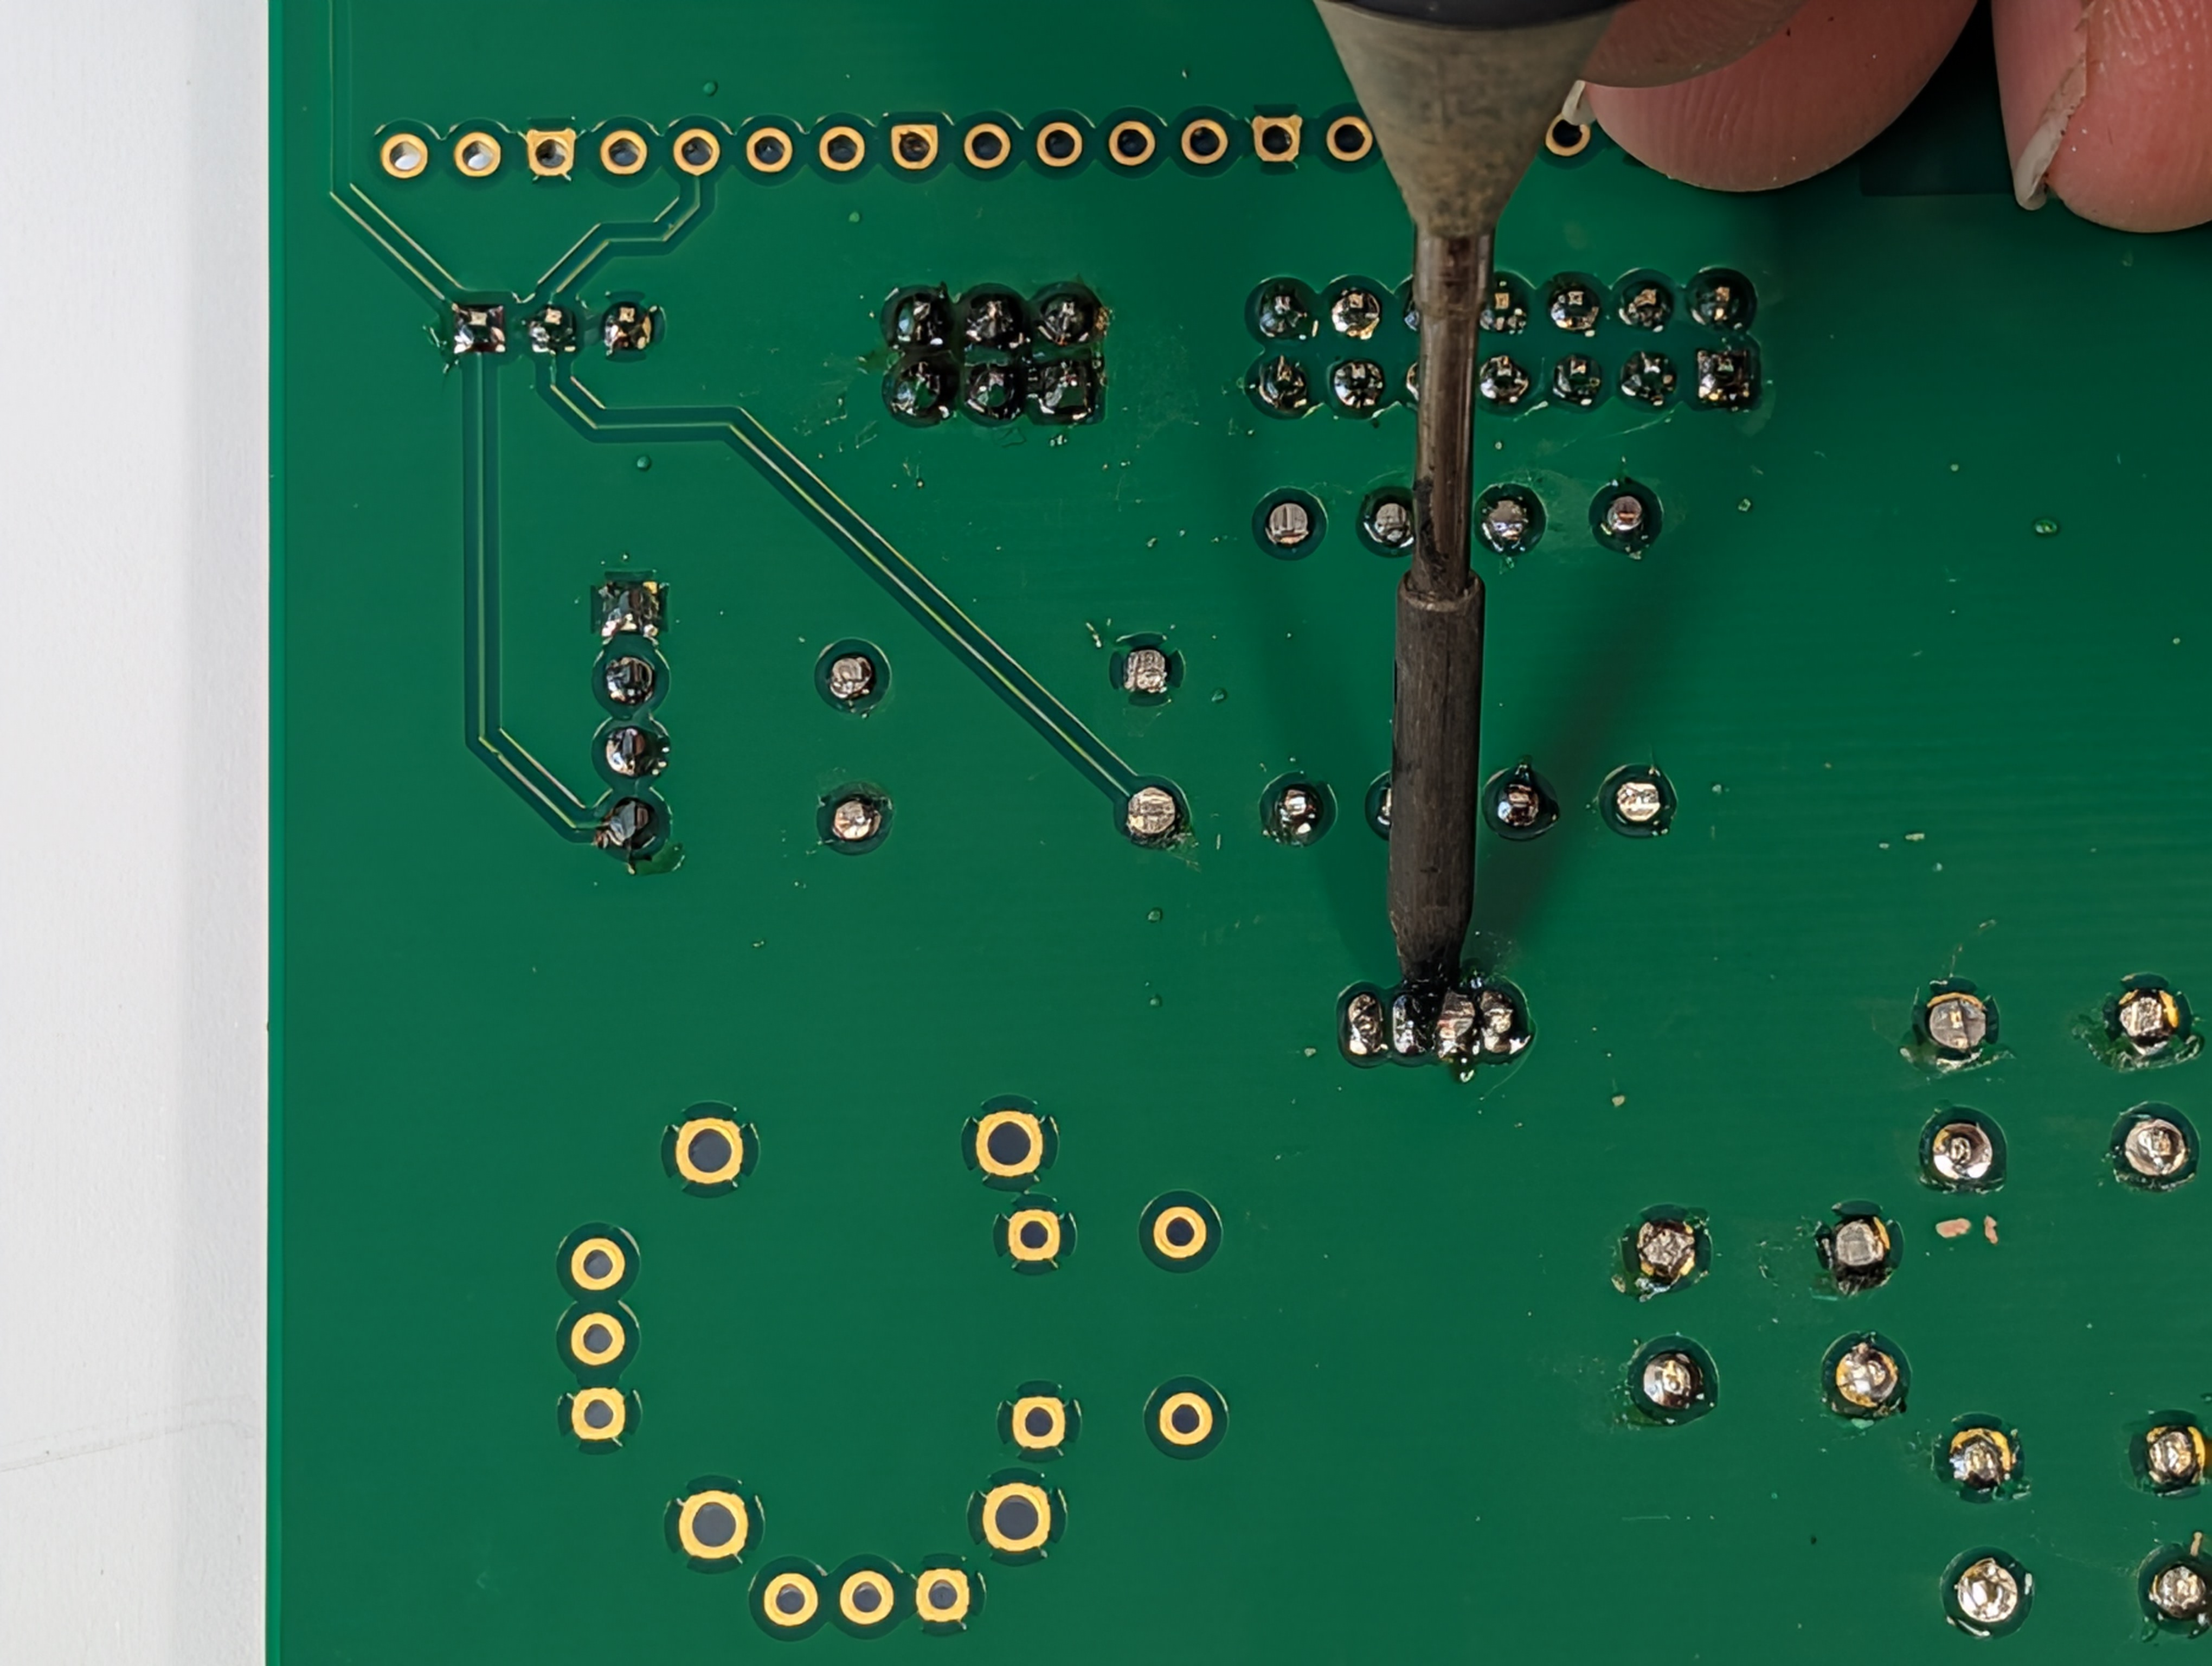
\includegraphics[width=0.75\textwidth]{pictures_of_construction/instruction_step_70.jpg}
\end{figure}

\begin{figure}[H]
    \centering
    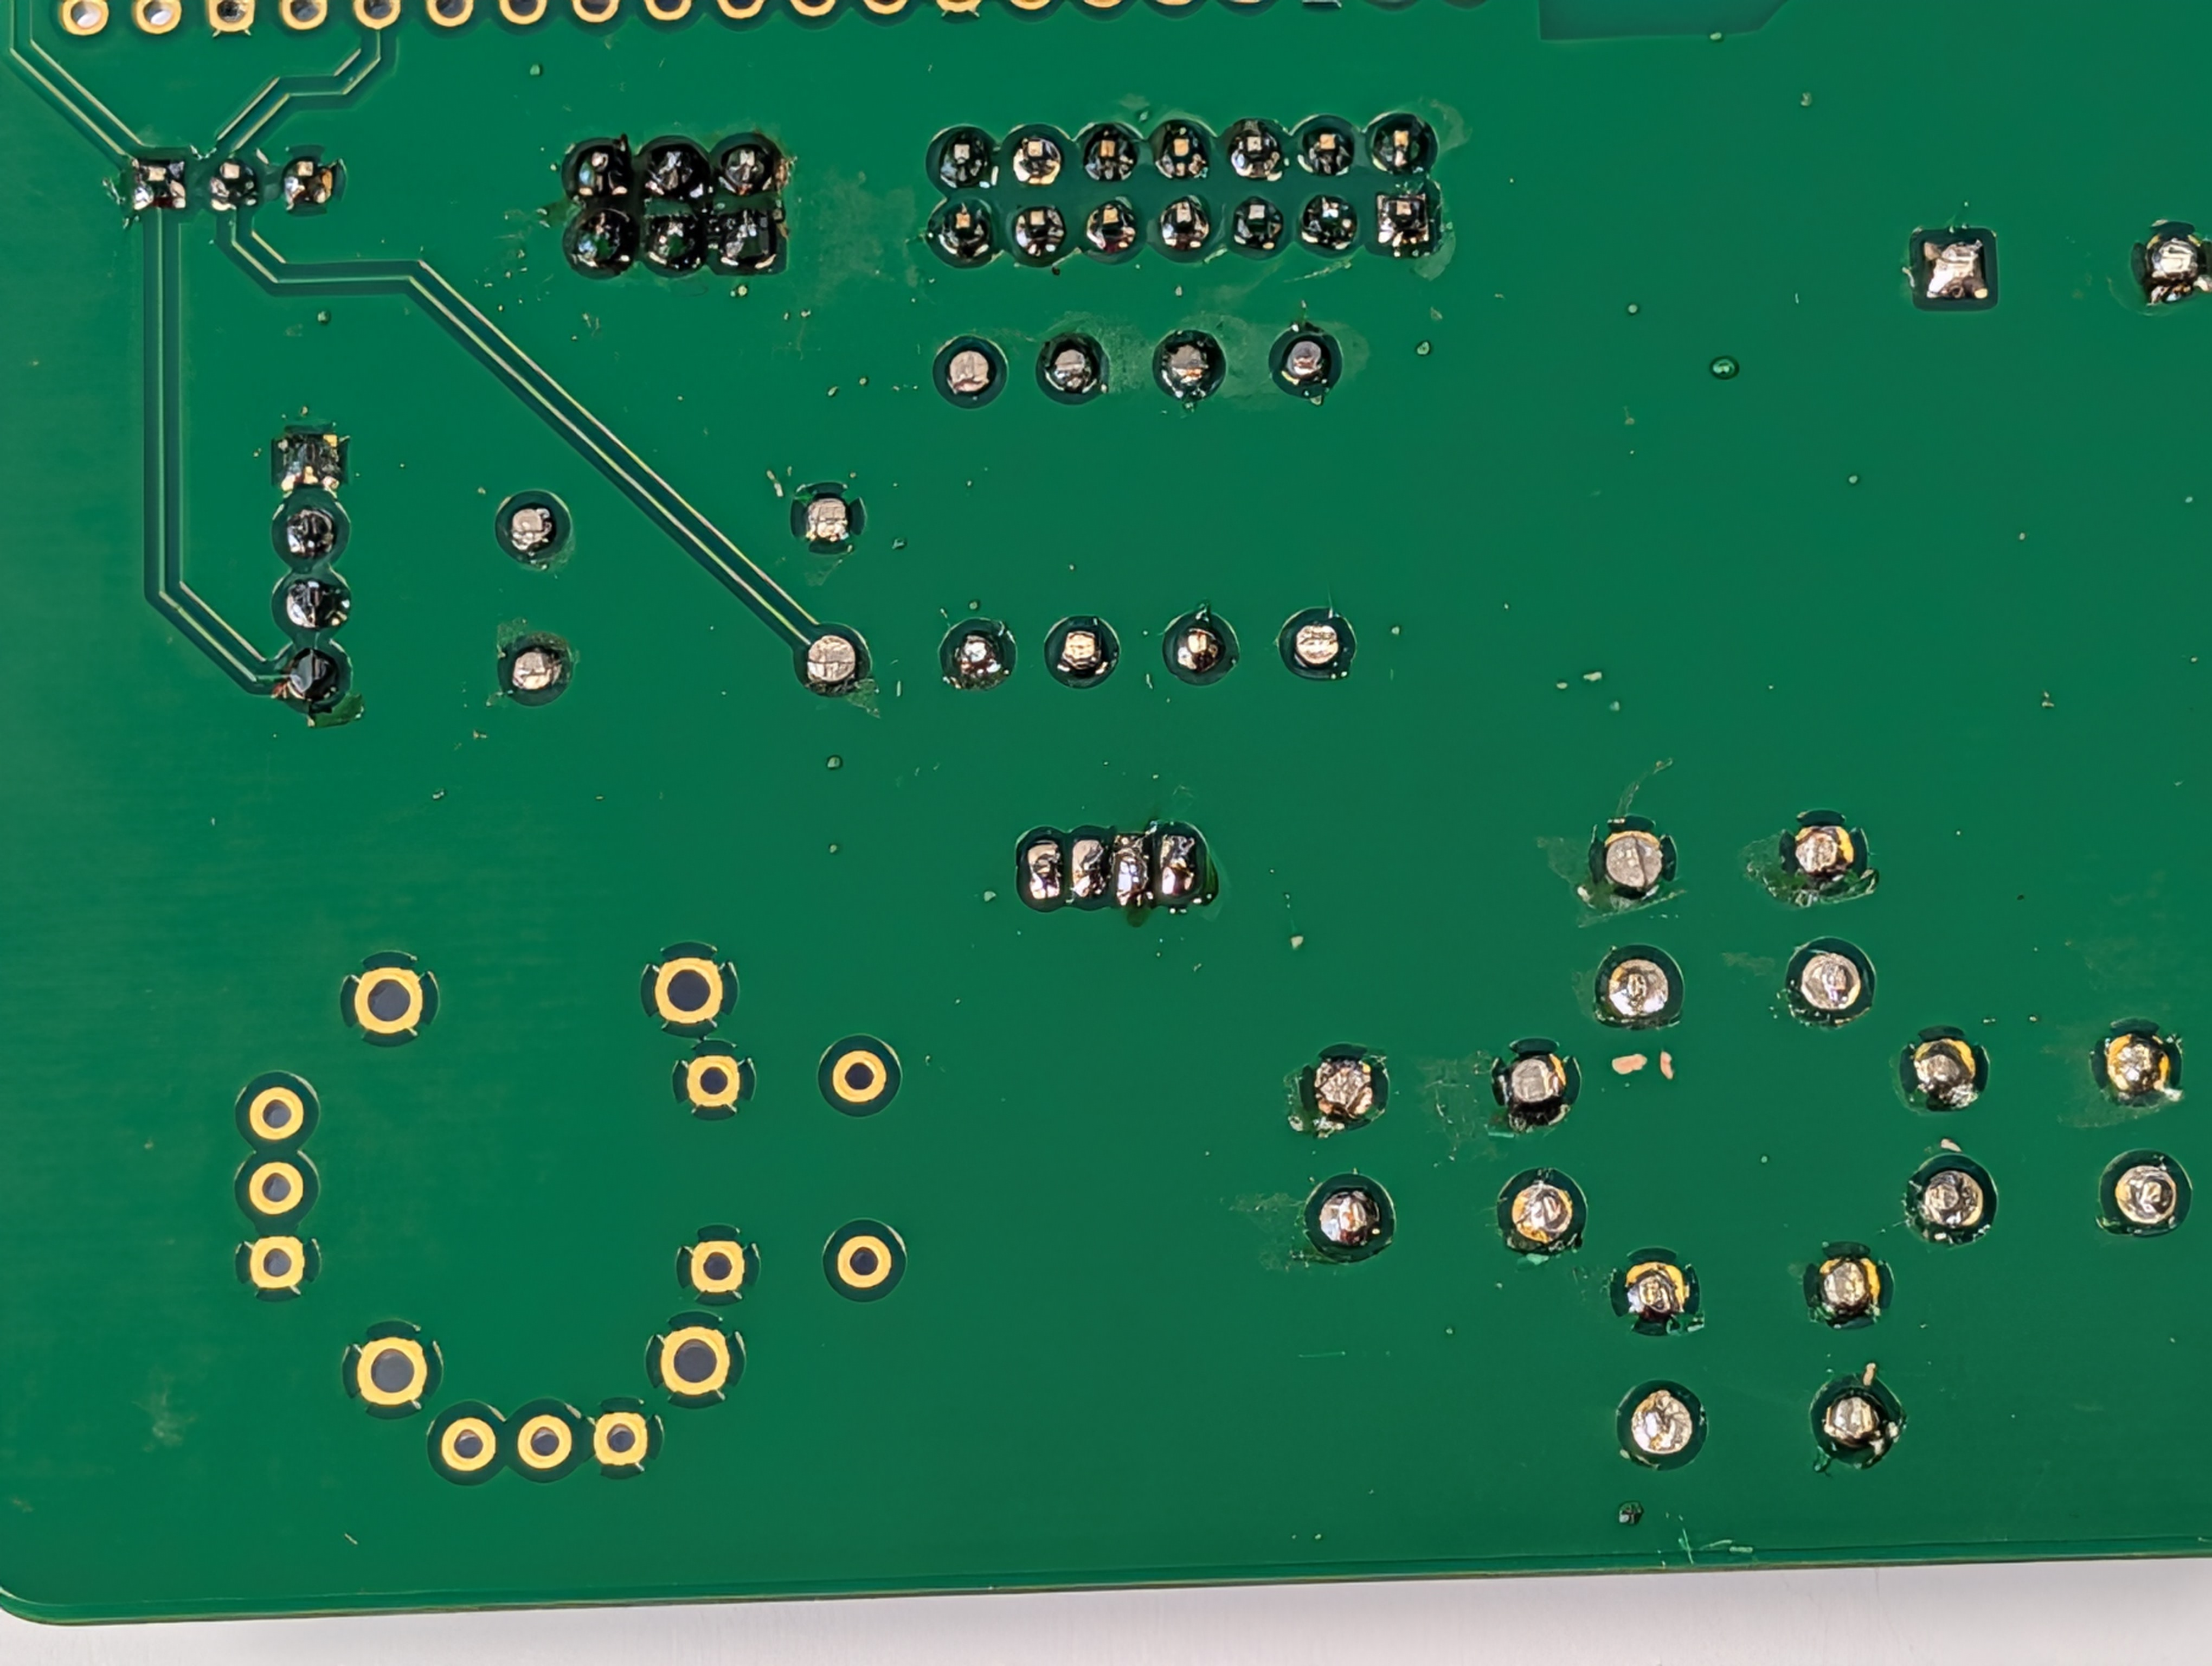
\includegraphics[width=0.75\textwidth]{pictures_of_construction/instruction_step_71.jpg}
\end{figure}

\subsection*{13. Raspberry Pi Pico einbauen}

Jetzt wird der vorbereitete Raspberry Pi Pico auf die Platine gesetzt.

So geht’s:
\begin{enumerate}
    \item Pico in die richtige Position stecken
    \item zuerst \textbf{zwei gegenüberliegende Pins} löten
    \item prüfen, ob alles gerade sitzt
    \item dann alle restlichen Pins löten
\end{enumerate}

\begin{figure}[H]
    \centering
    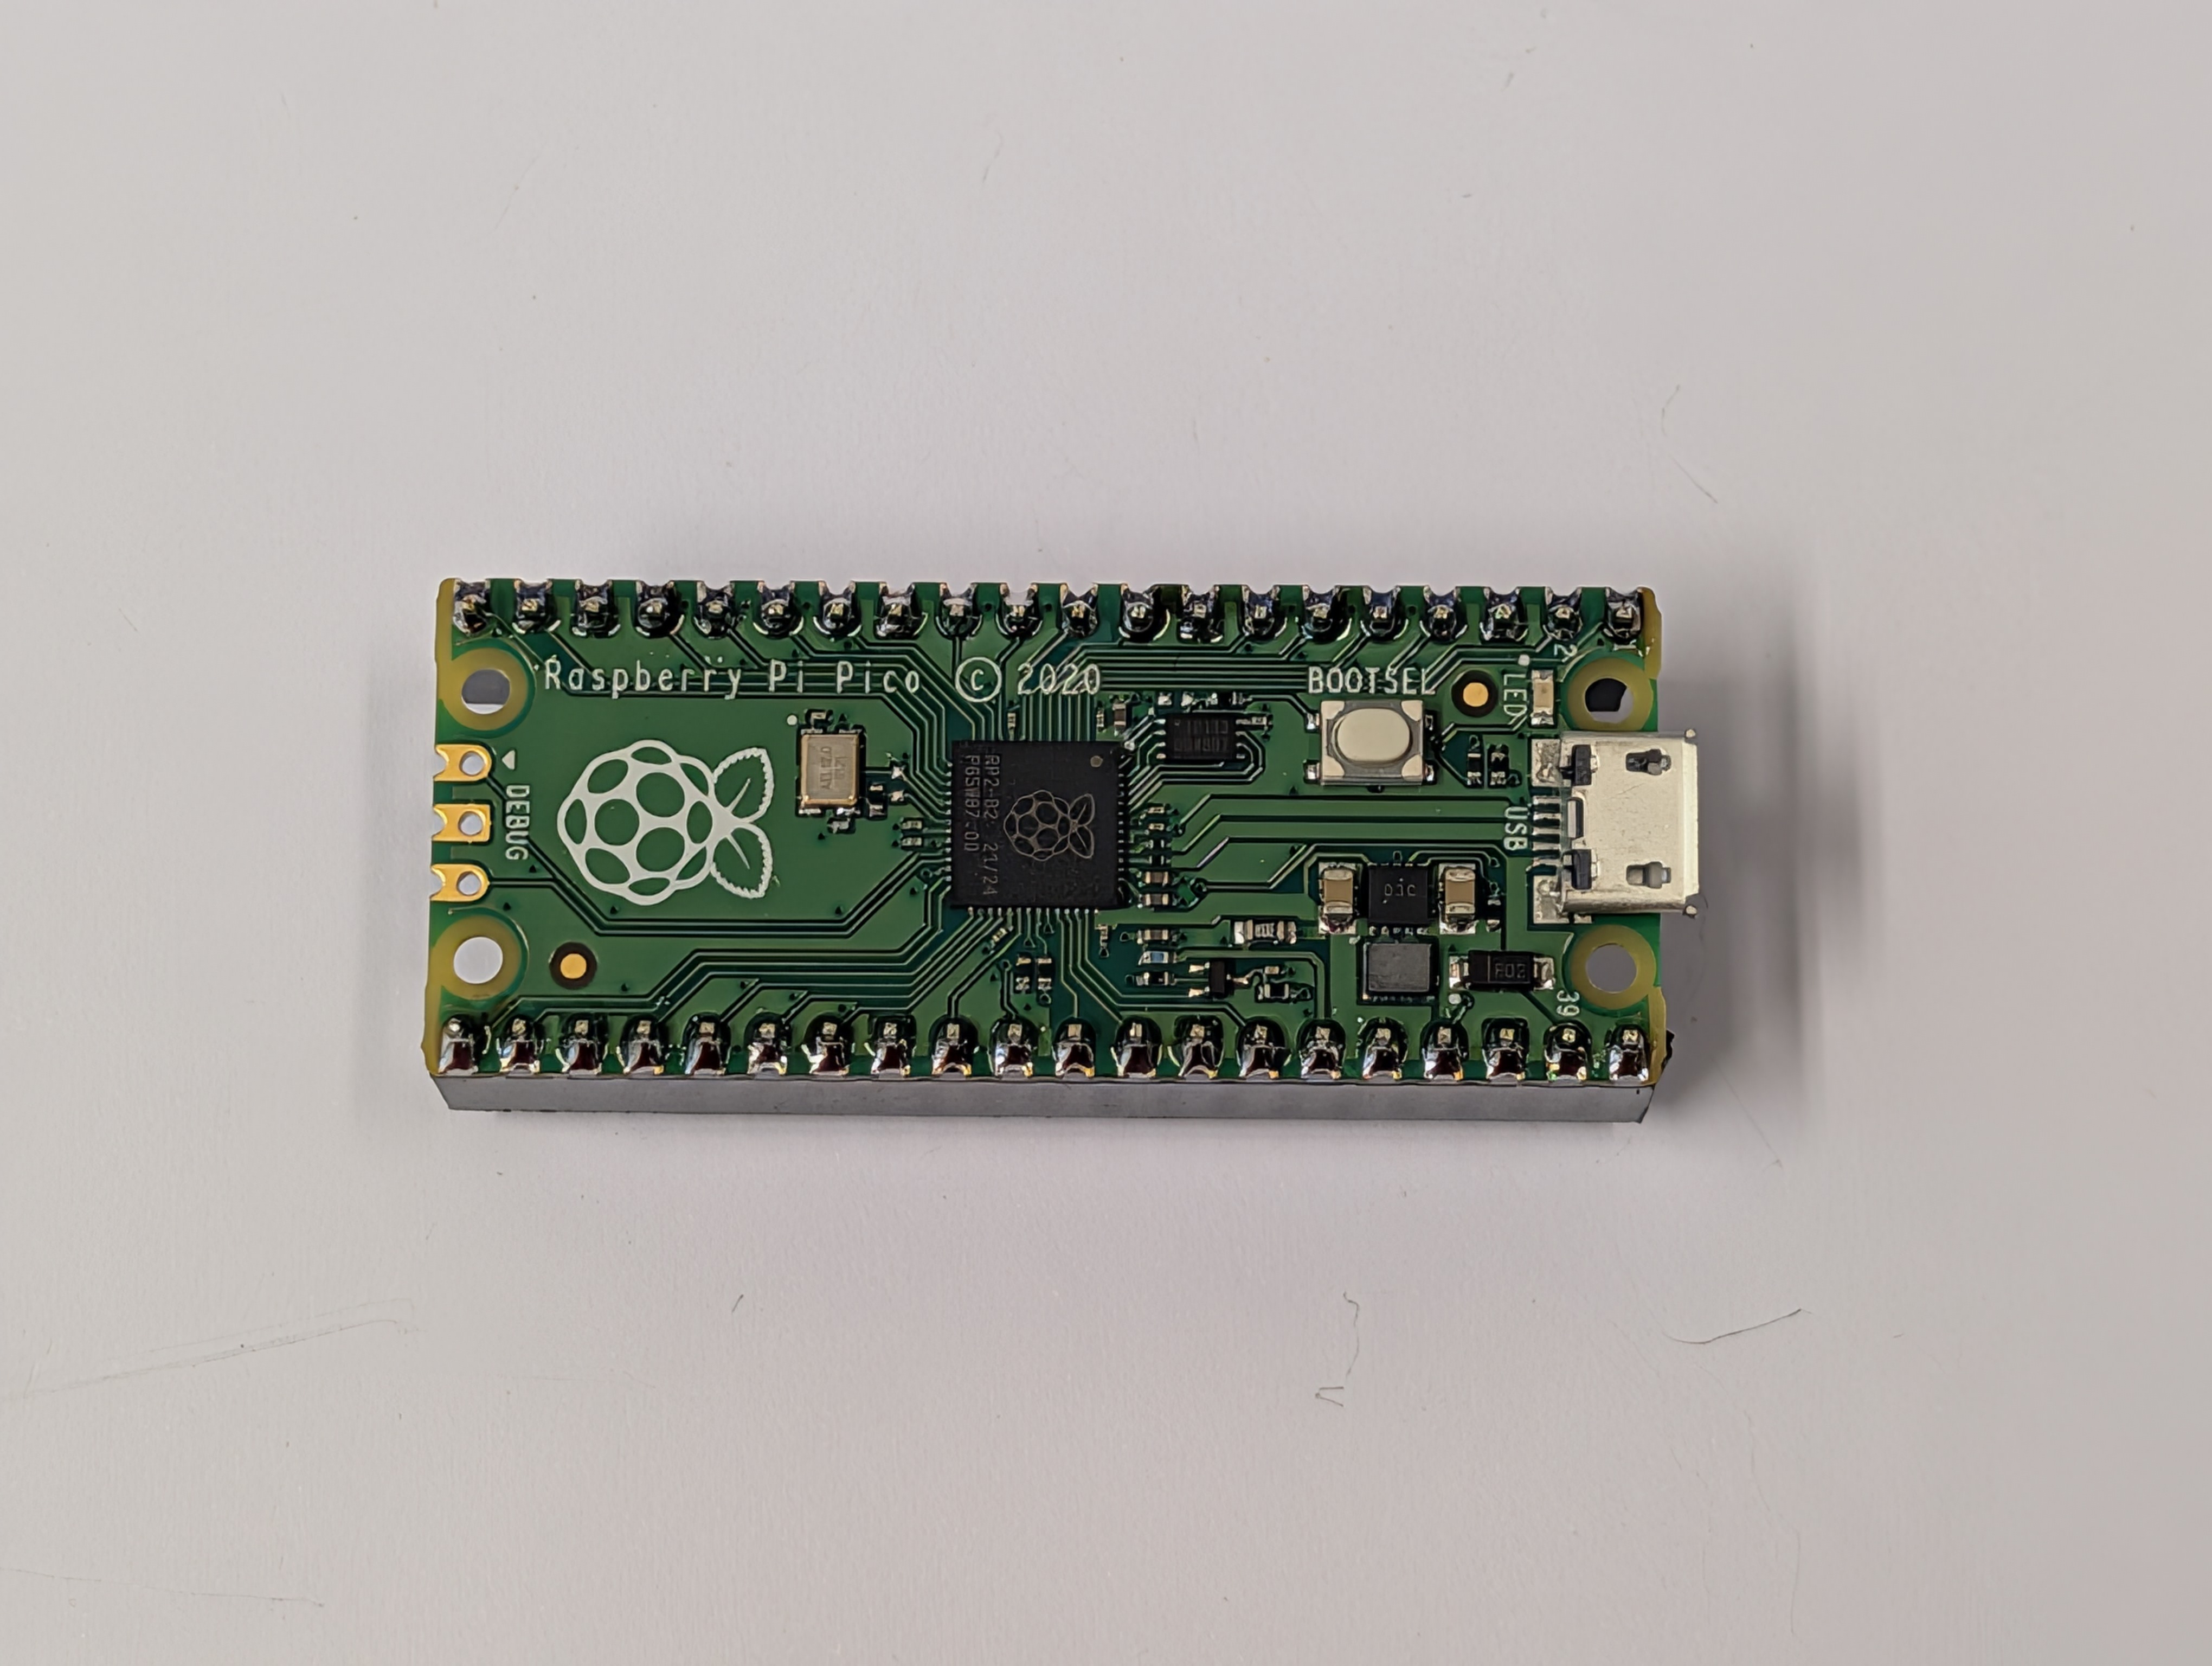
\includegraphics[width=0.75\textwidth]{pictures_of_construction/instruction_step_72.jpg}
\end{figure}

\begin{figure}[H]
    \centering
    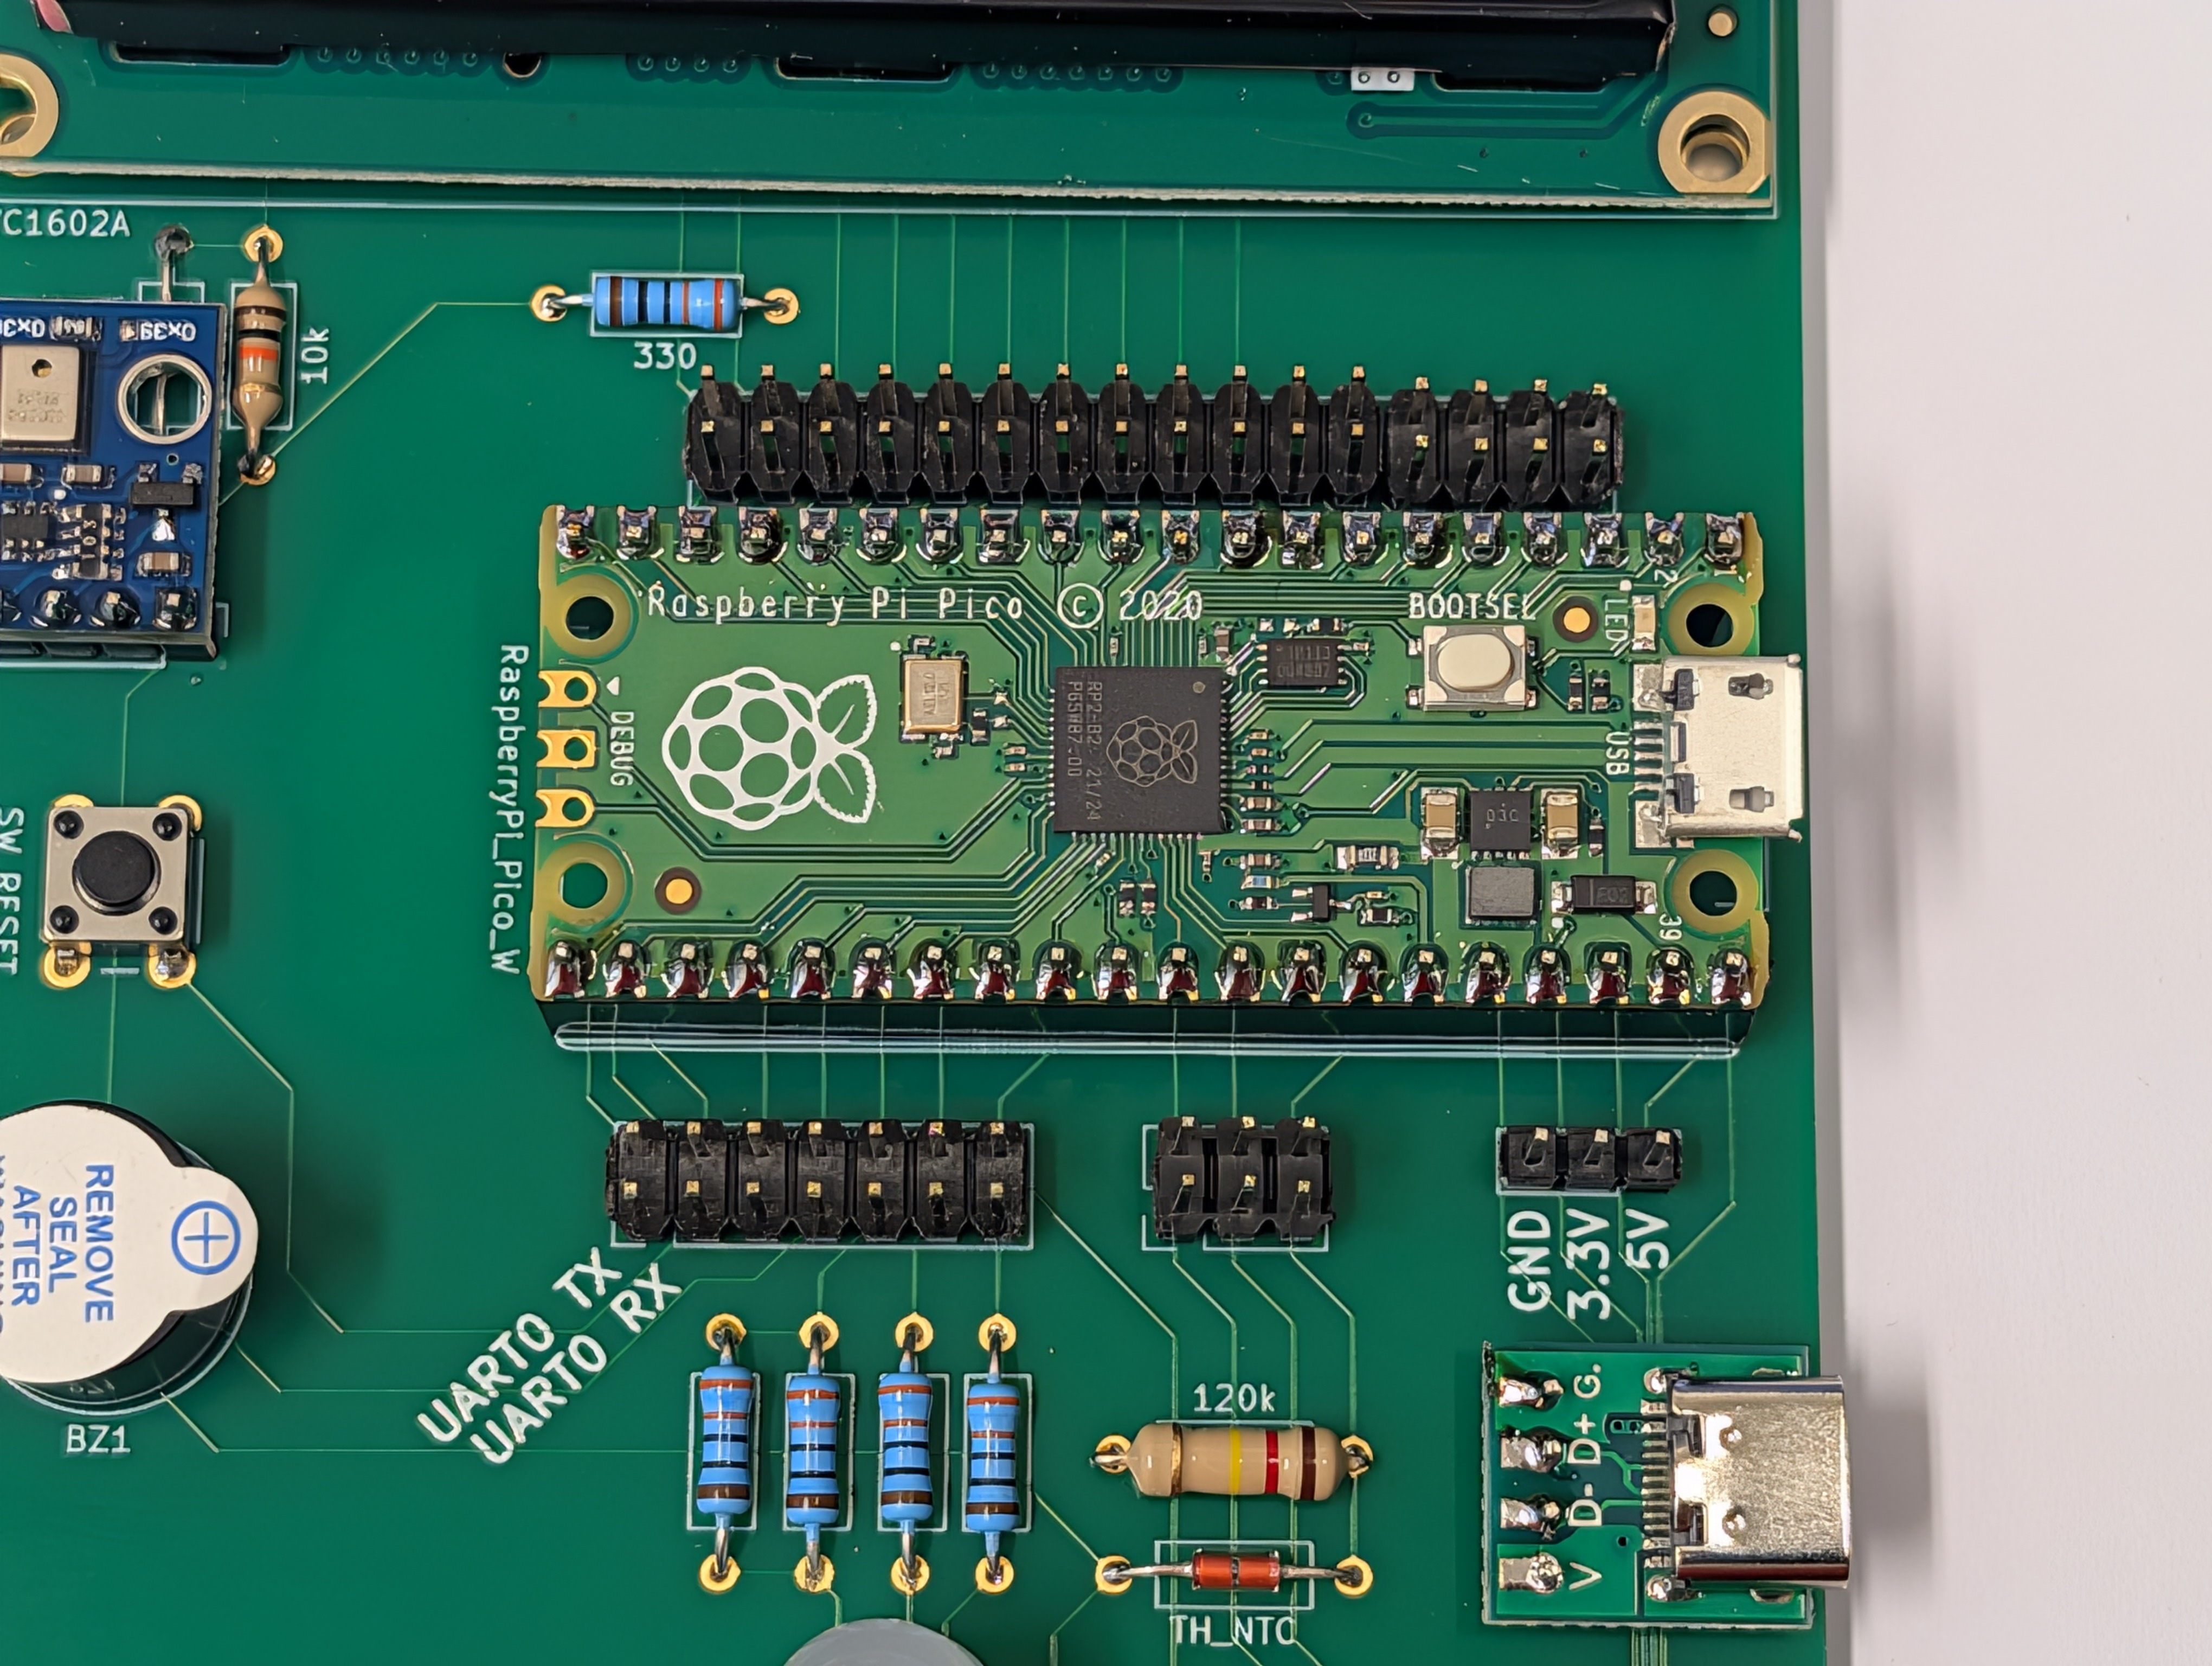
\includegraphics[width=0.75\textwidth]{pictures_of_construction/instruction_step_73.jpg}
\end{figure}

\begin{figure}[H]
    \centering
    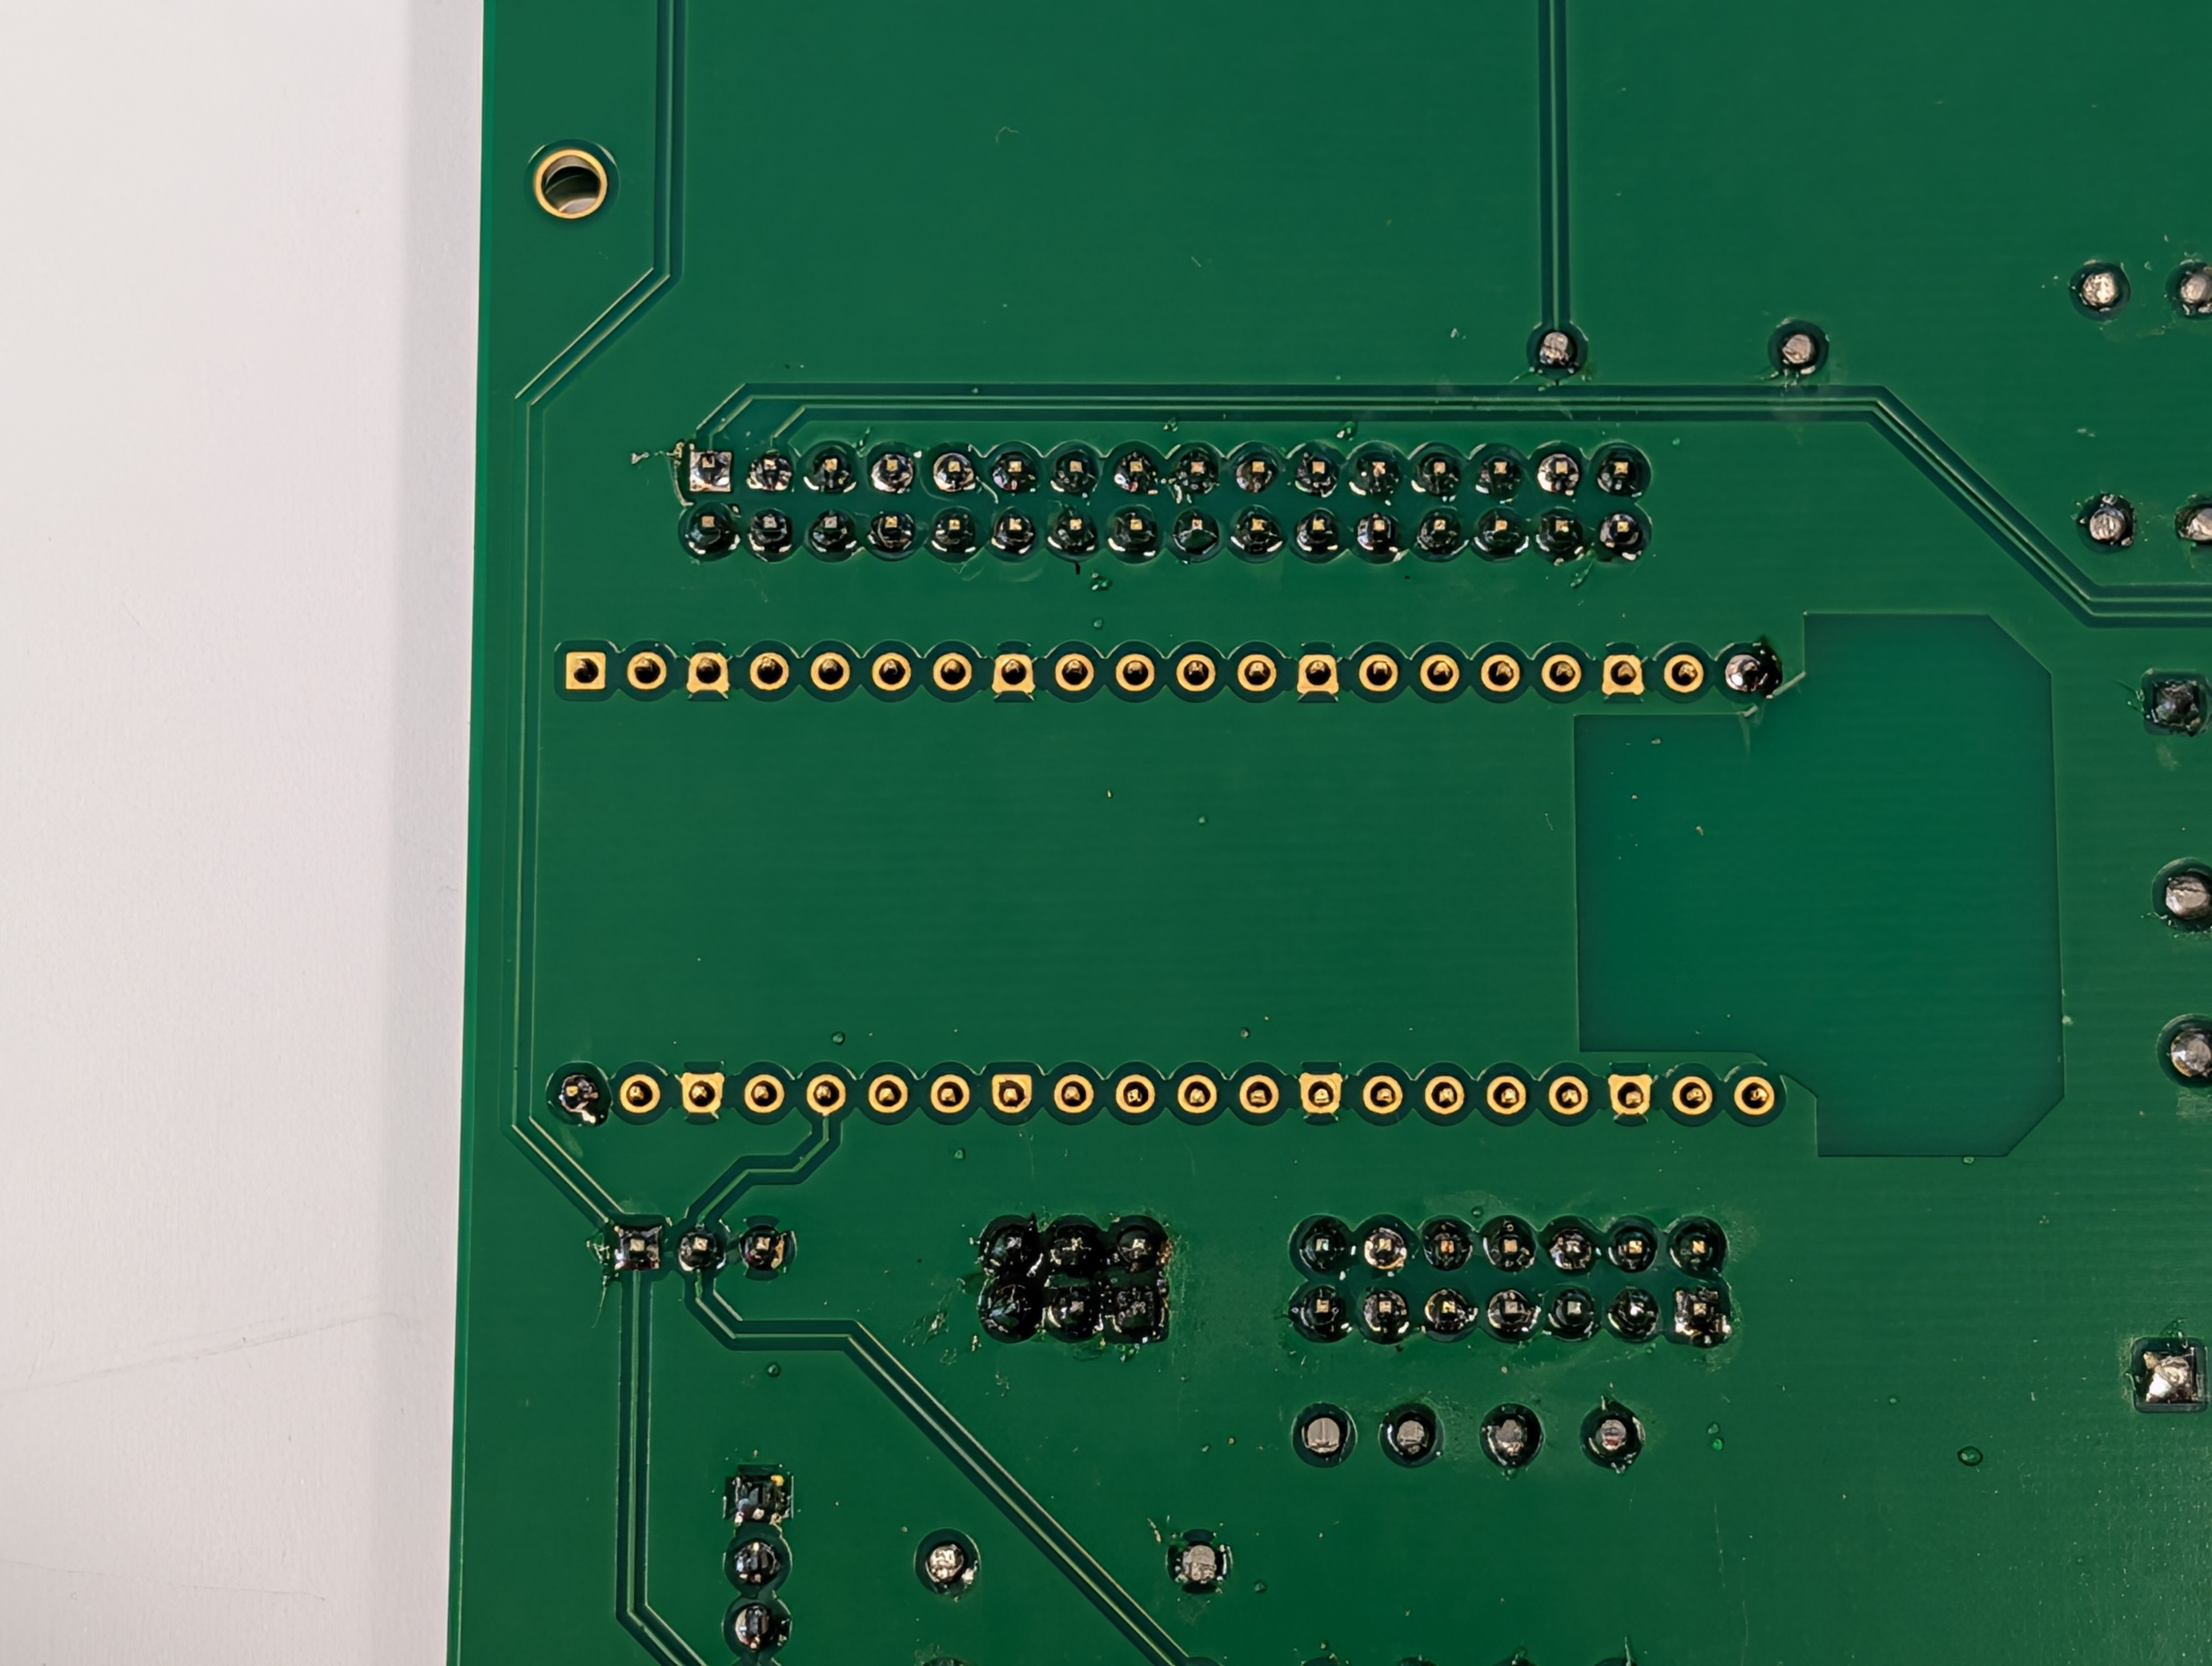
\includegraphics[width=0.75\textwidth]{pictures_of_construction/instruction_step_74.jpg}
\end{figure}

\subsection*{14. Joystick einbauen}

Der Joystick kommt ganz zum Schluss.

Er hat viele Pins. Deshalb ist dieser Schritt etwas knifflig.

So geht’s:
\begin{enumerate}
    \item Setze zuerst die passenden Pins vorsichtig in die Löcher ein.
    \item Bewege den Joystick langsam ein wenig hin und her, bis alle Pins richtig sitzen.
    \item Drücke ihn ganz hinein.
    \item Löte dann alle Pins fest.
\end{enumerate}

\begin{figure}[H]
    \centering
    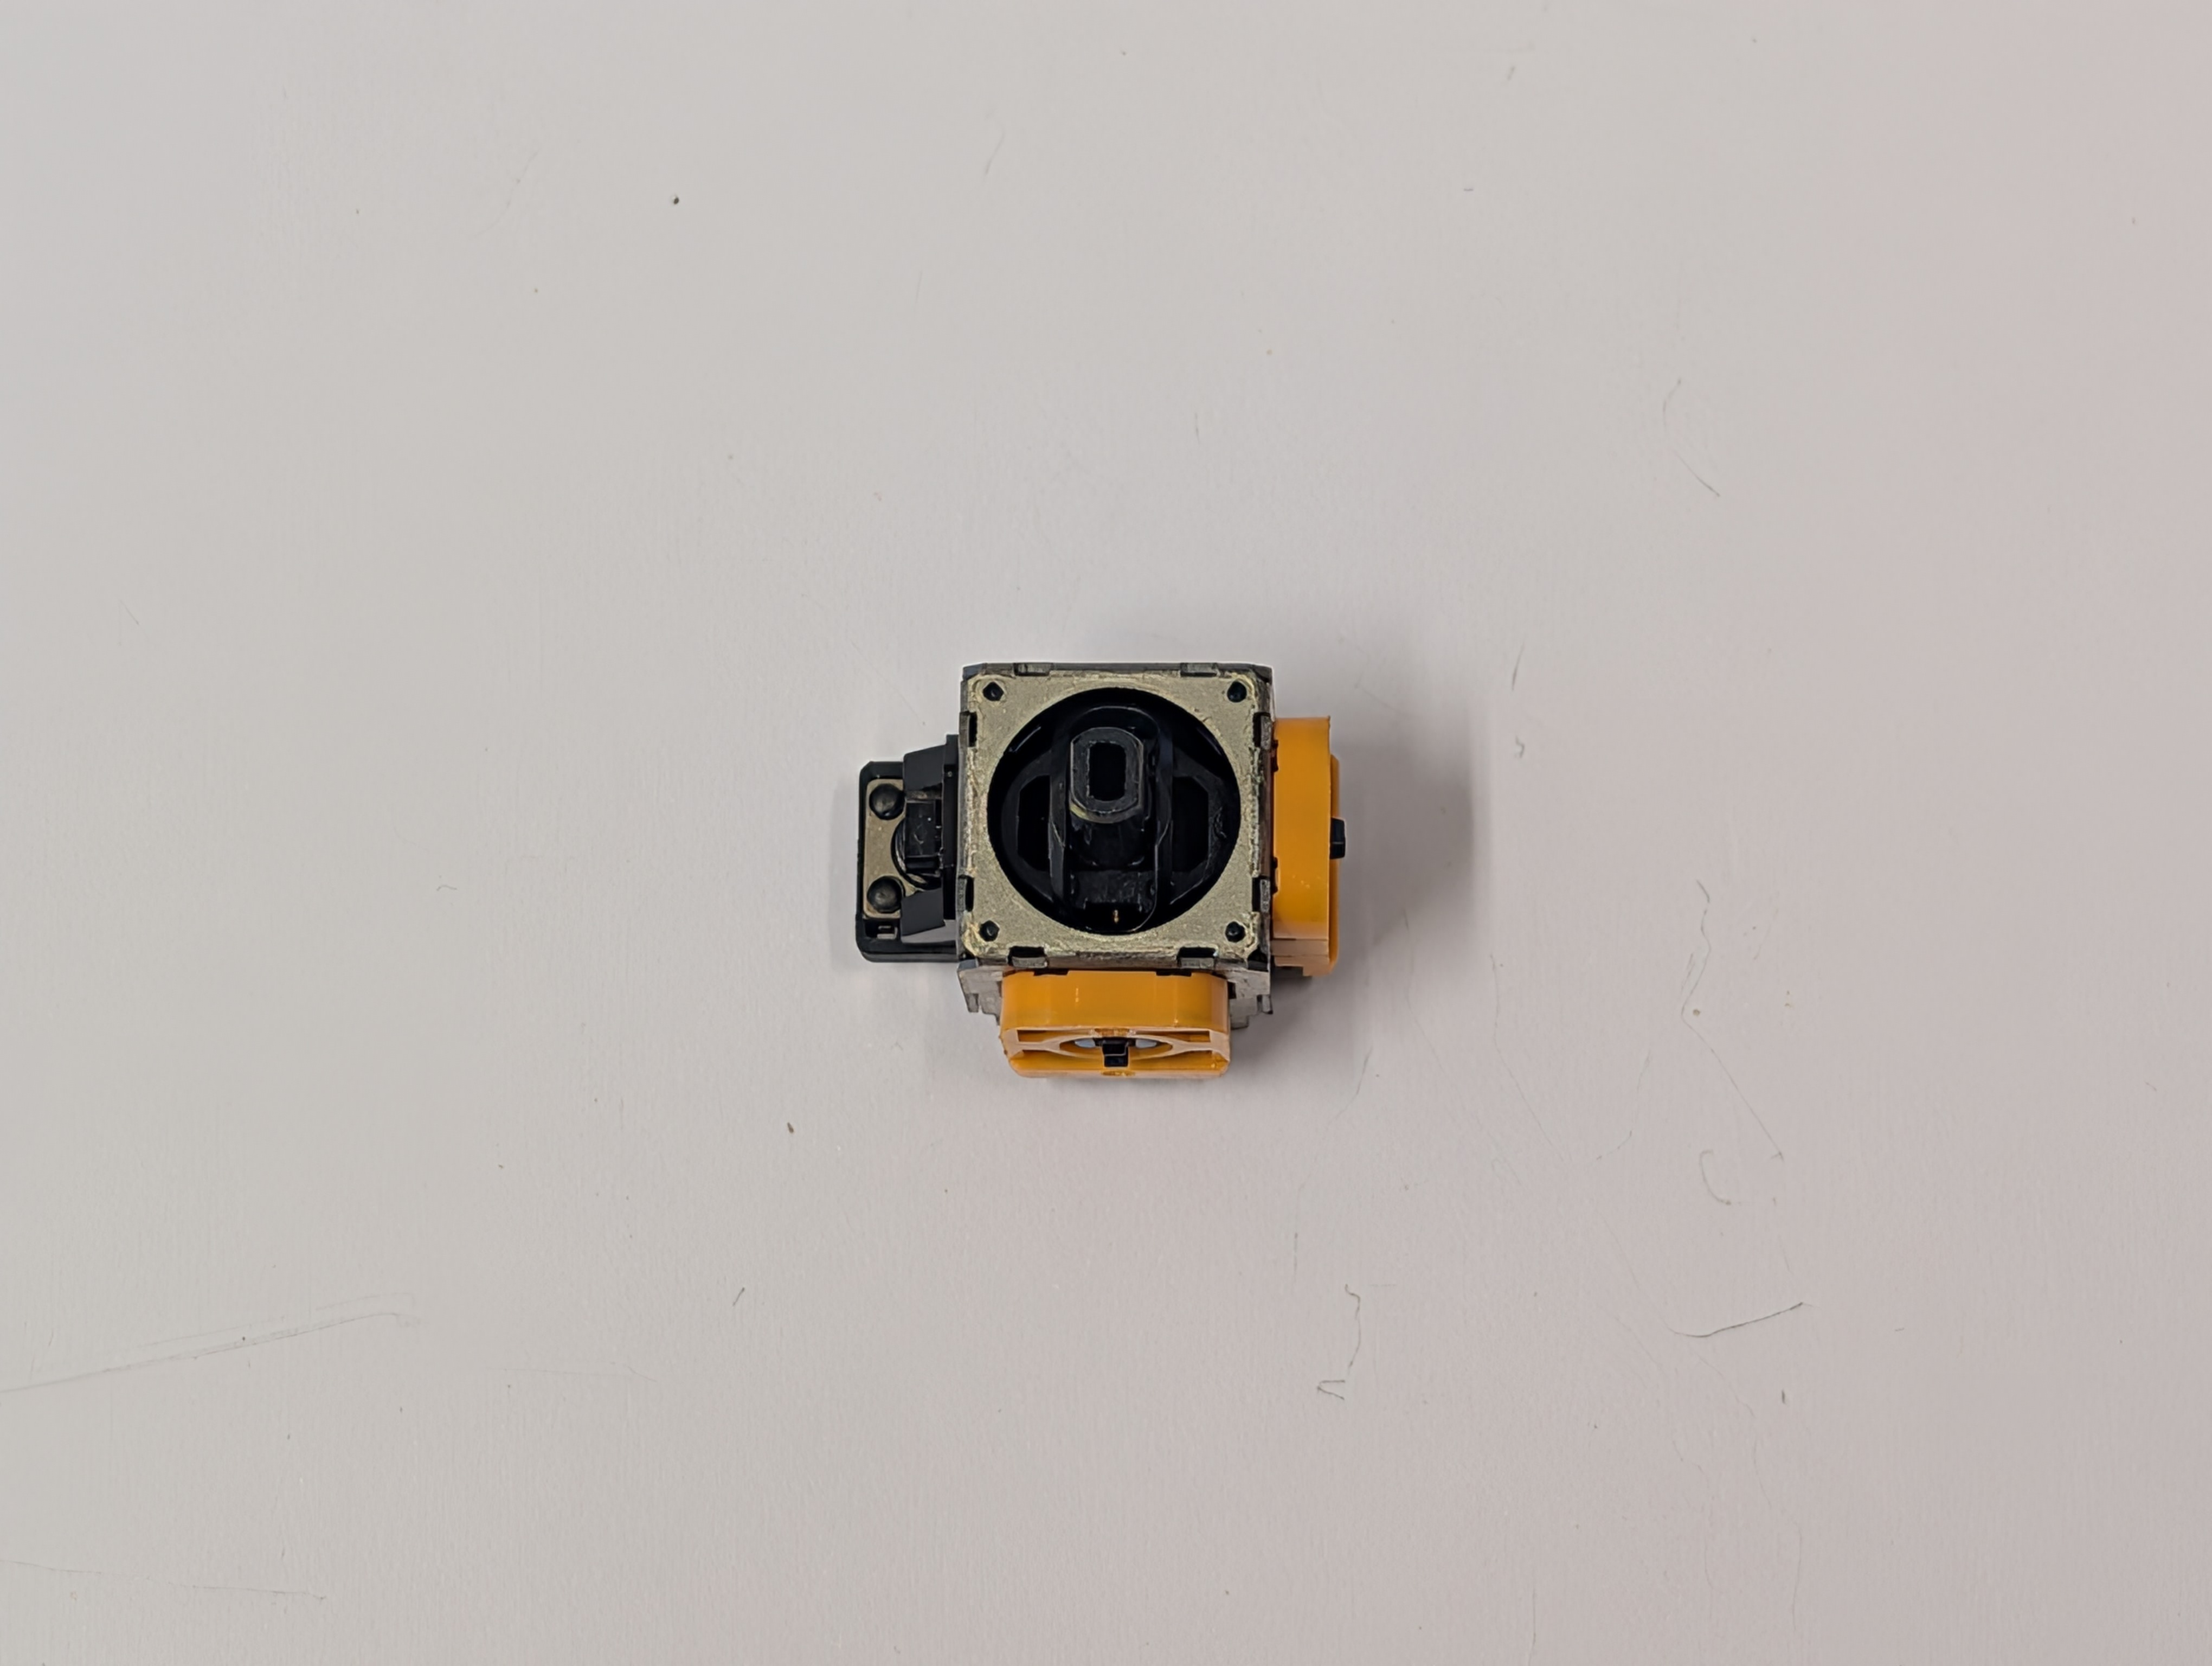
\includegraphics[width=0.75\textwidth]{pictures_of_construction/instruction_step_75.jpg}
\end{figure}

\begin{figure}[H]
    \centering
    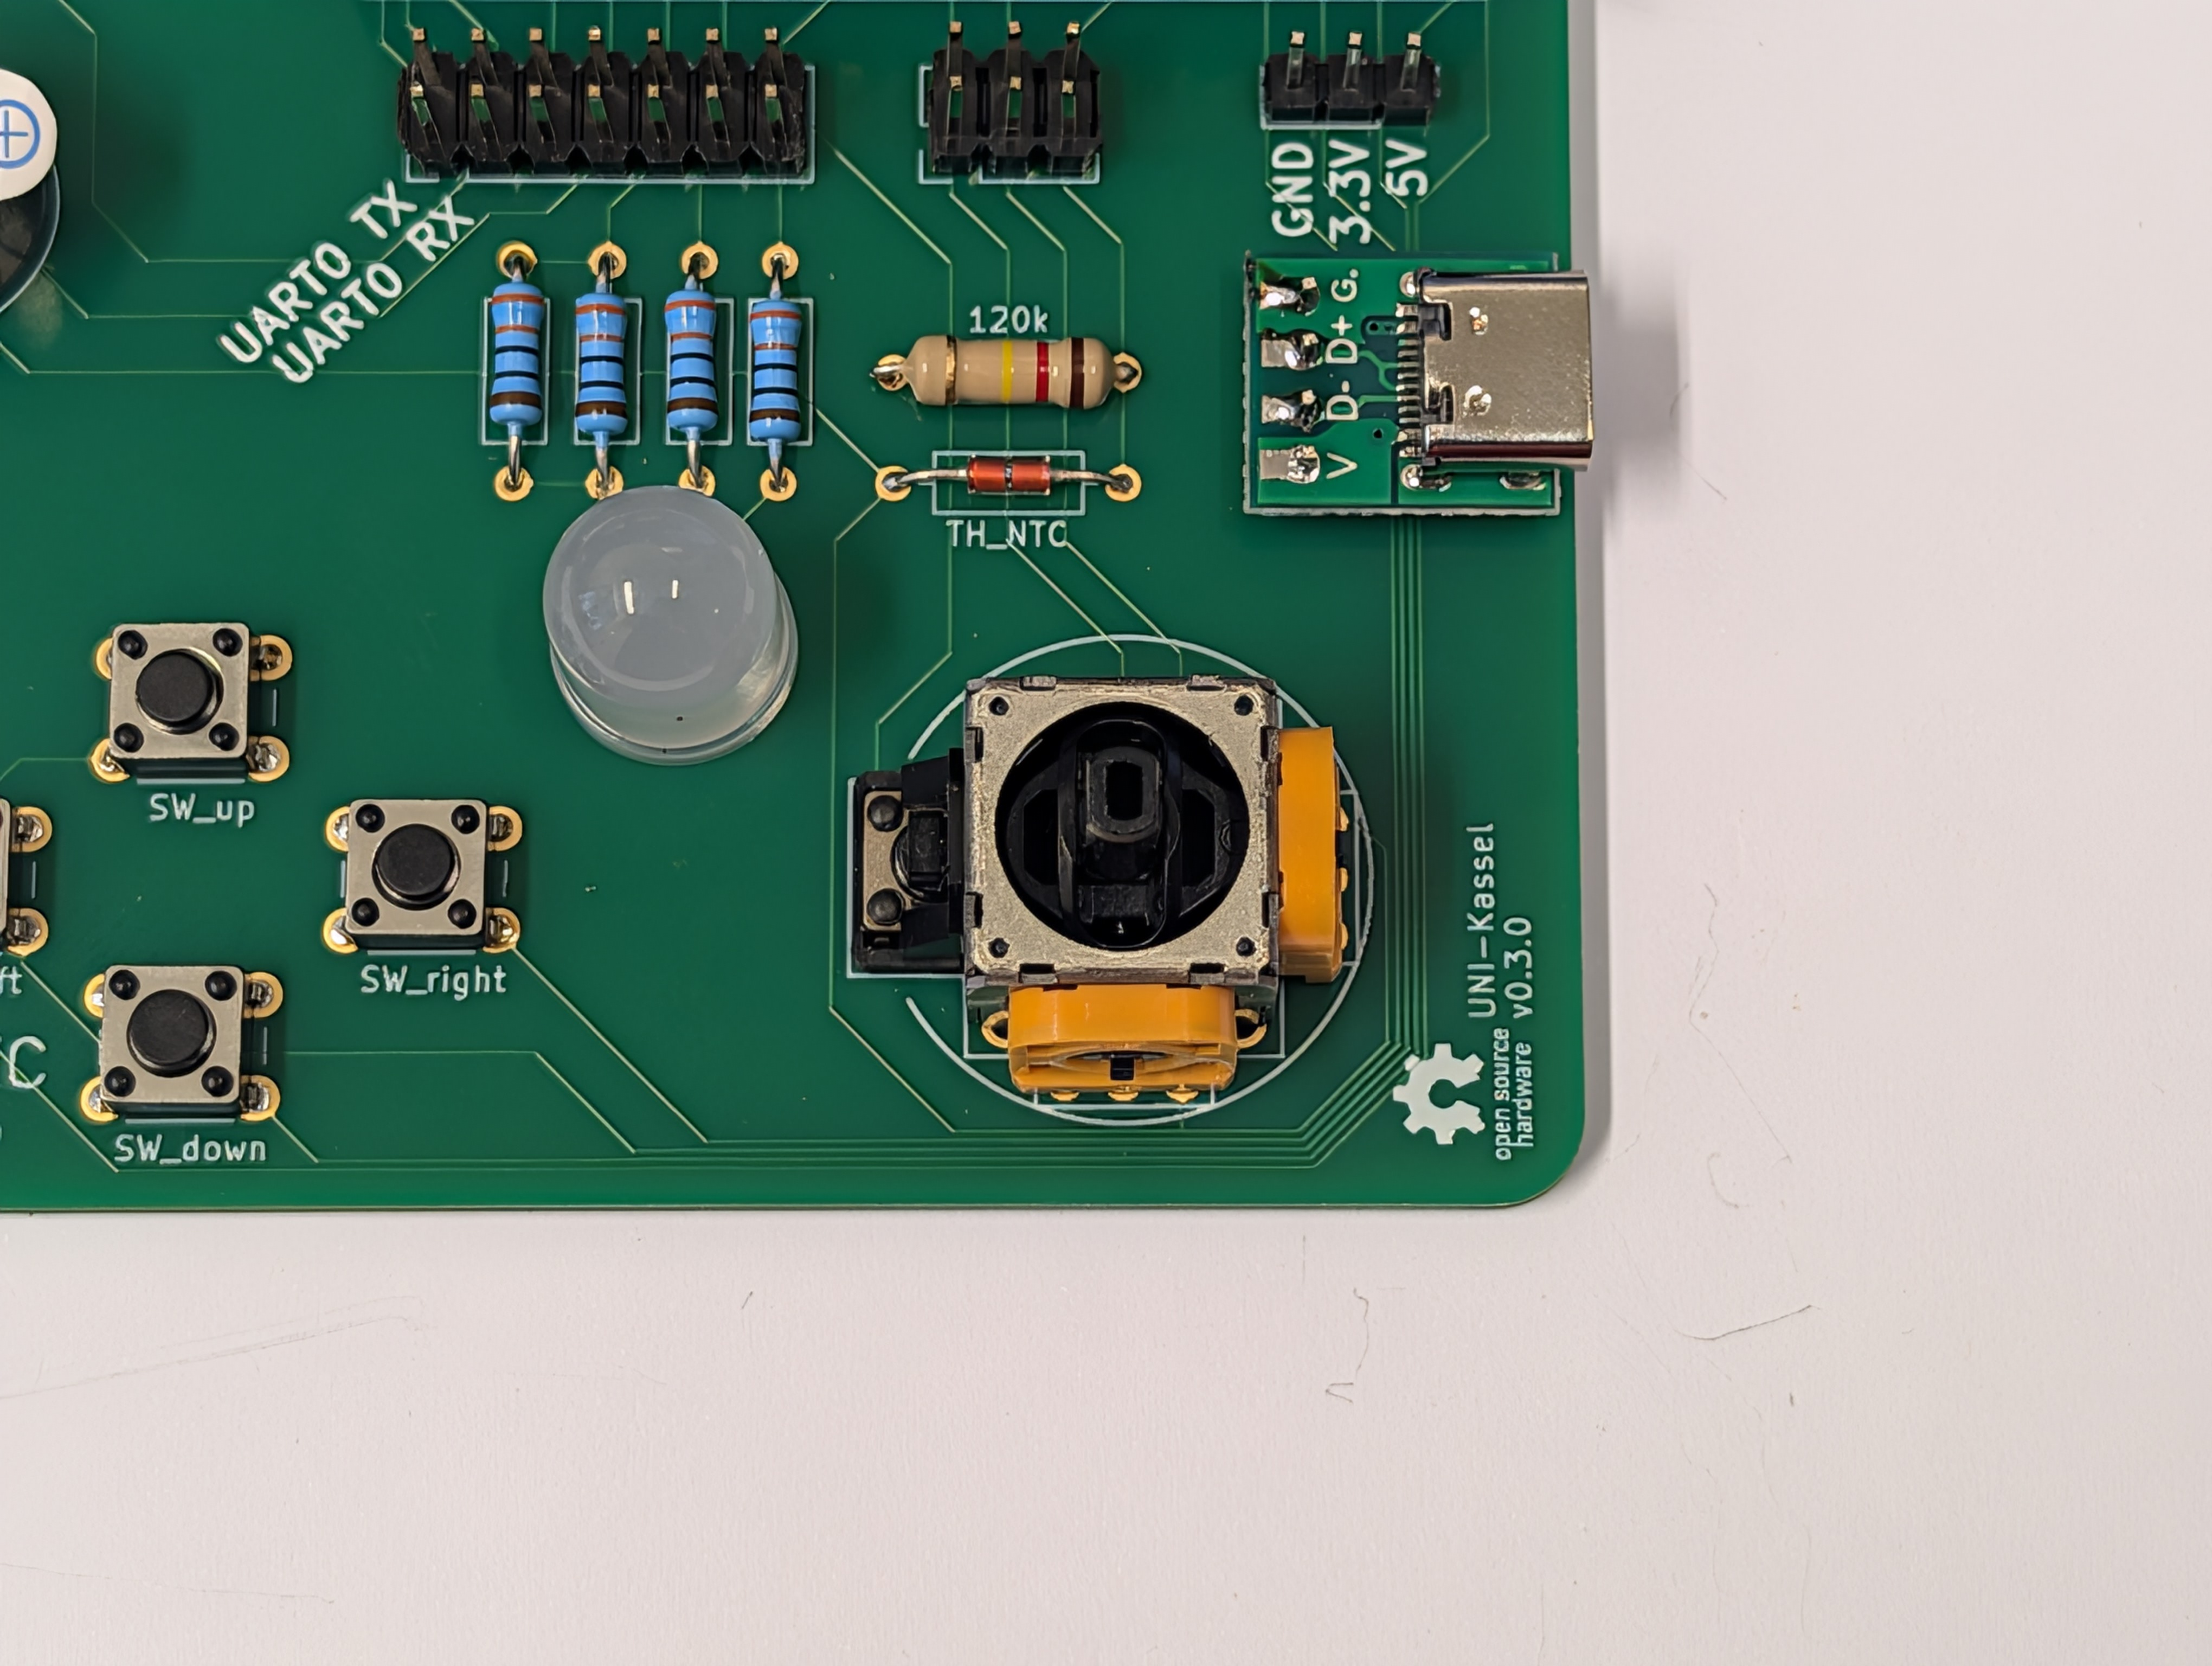
\includegraphics[width=0.75\textwidth]{pictures_of_construction/instruction_step_76.jpg}
\end{figure}

\begin{figure}[H]
    \centering
    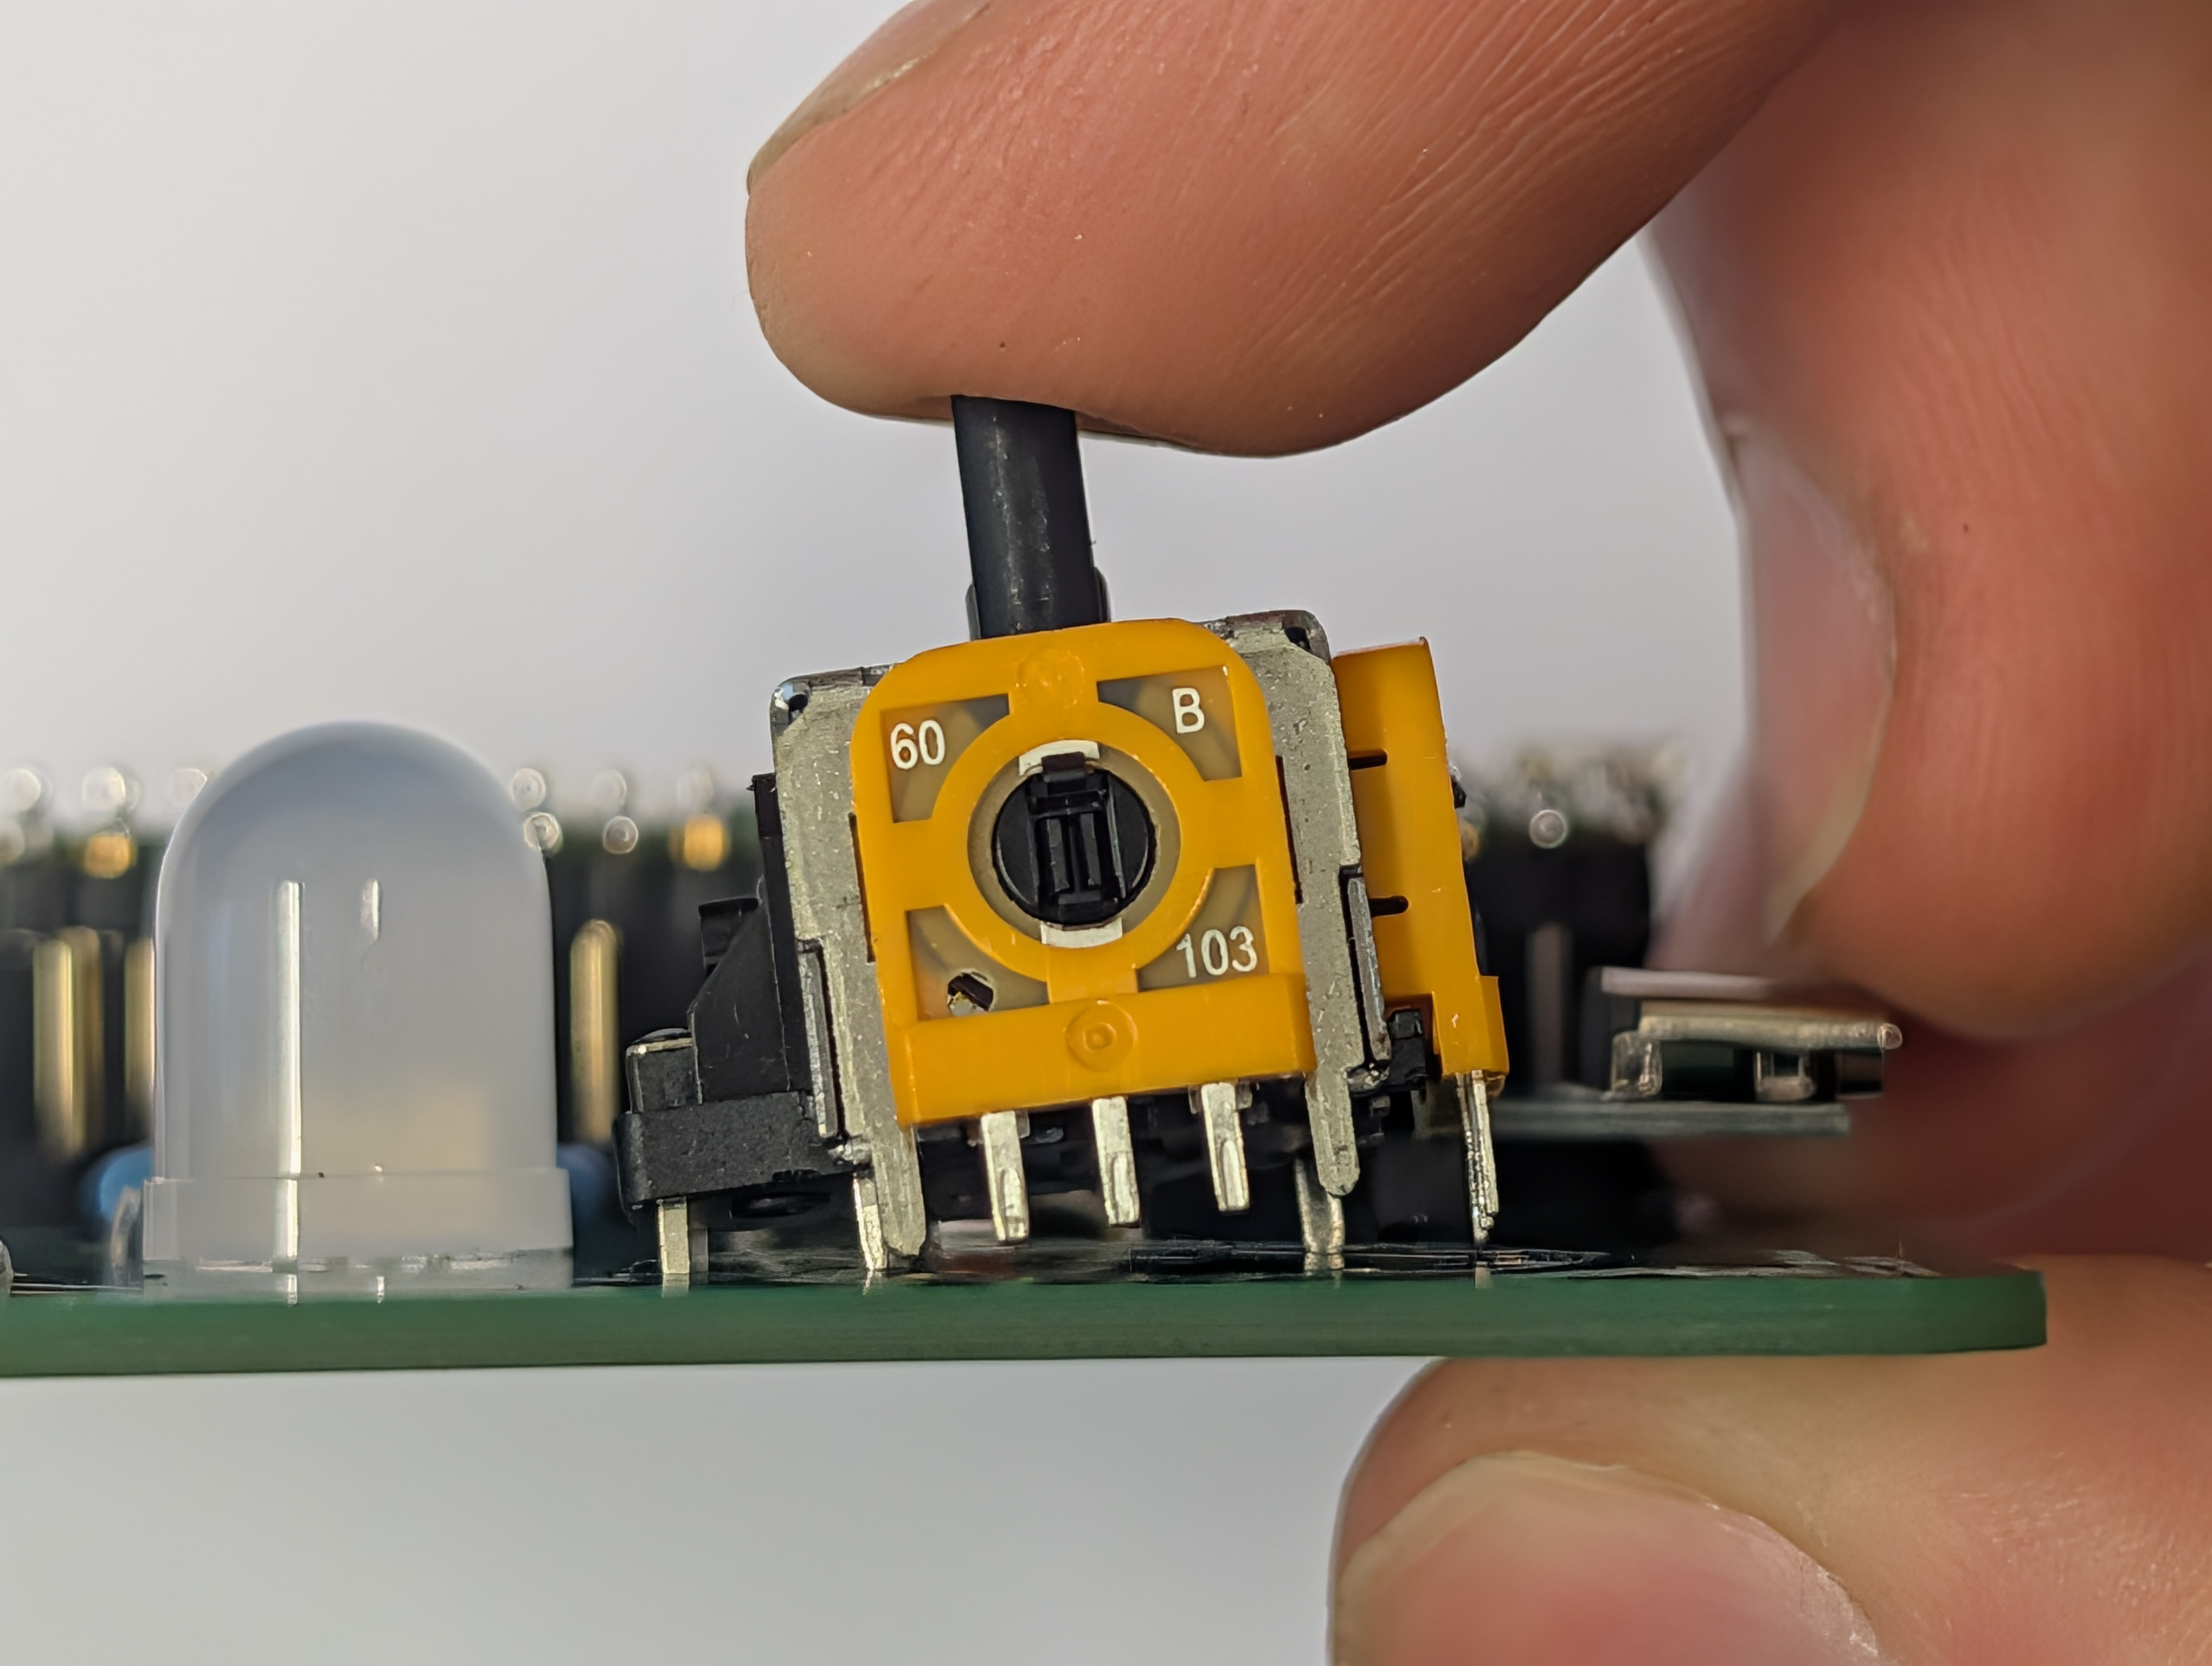
\includegraphics[width=0.75\textwidth]{pictures_of_construction/instruction_step_77.jpg}
\end{figure}

\begin{figure}[H]
    \centering
    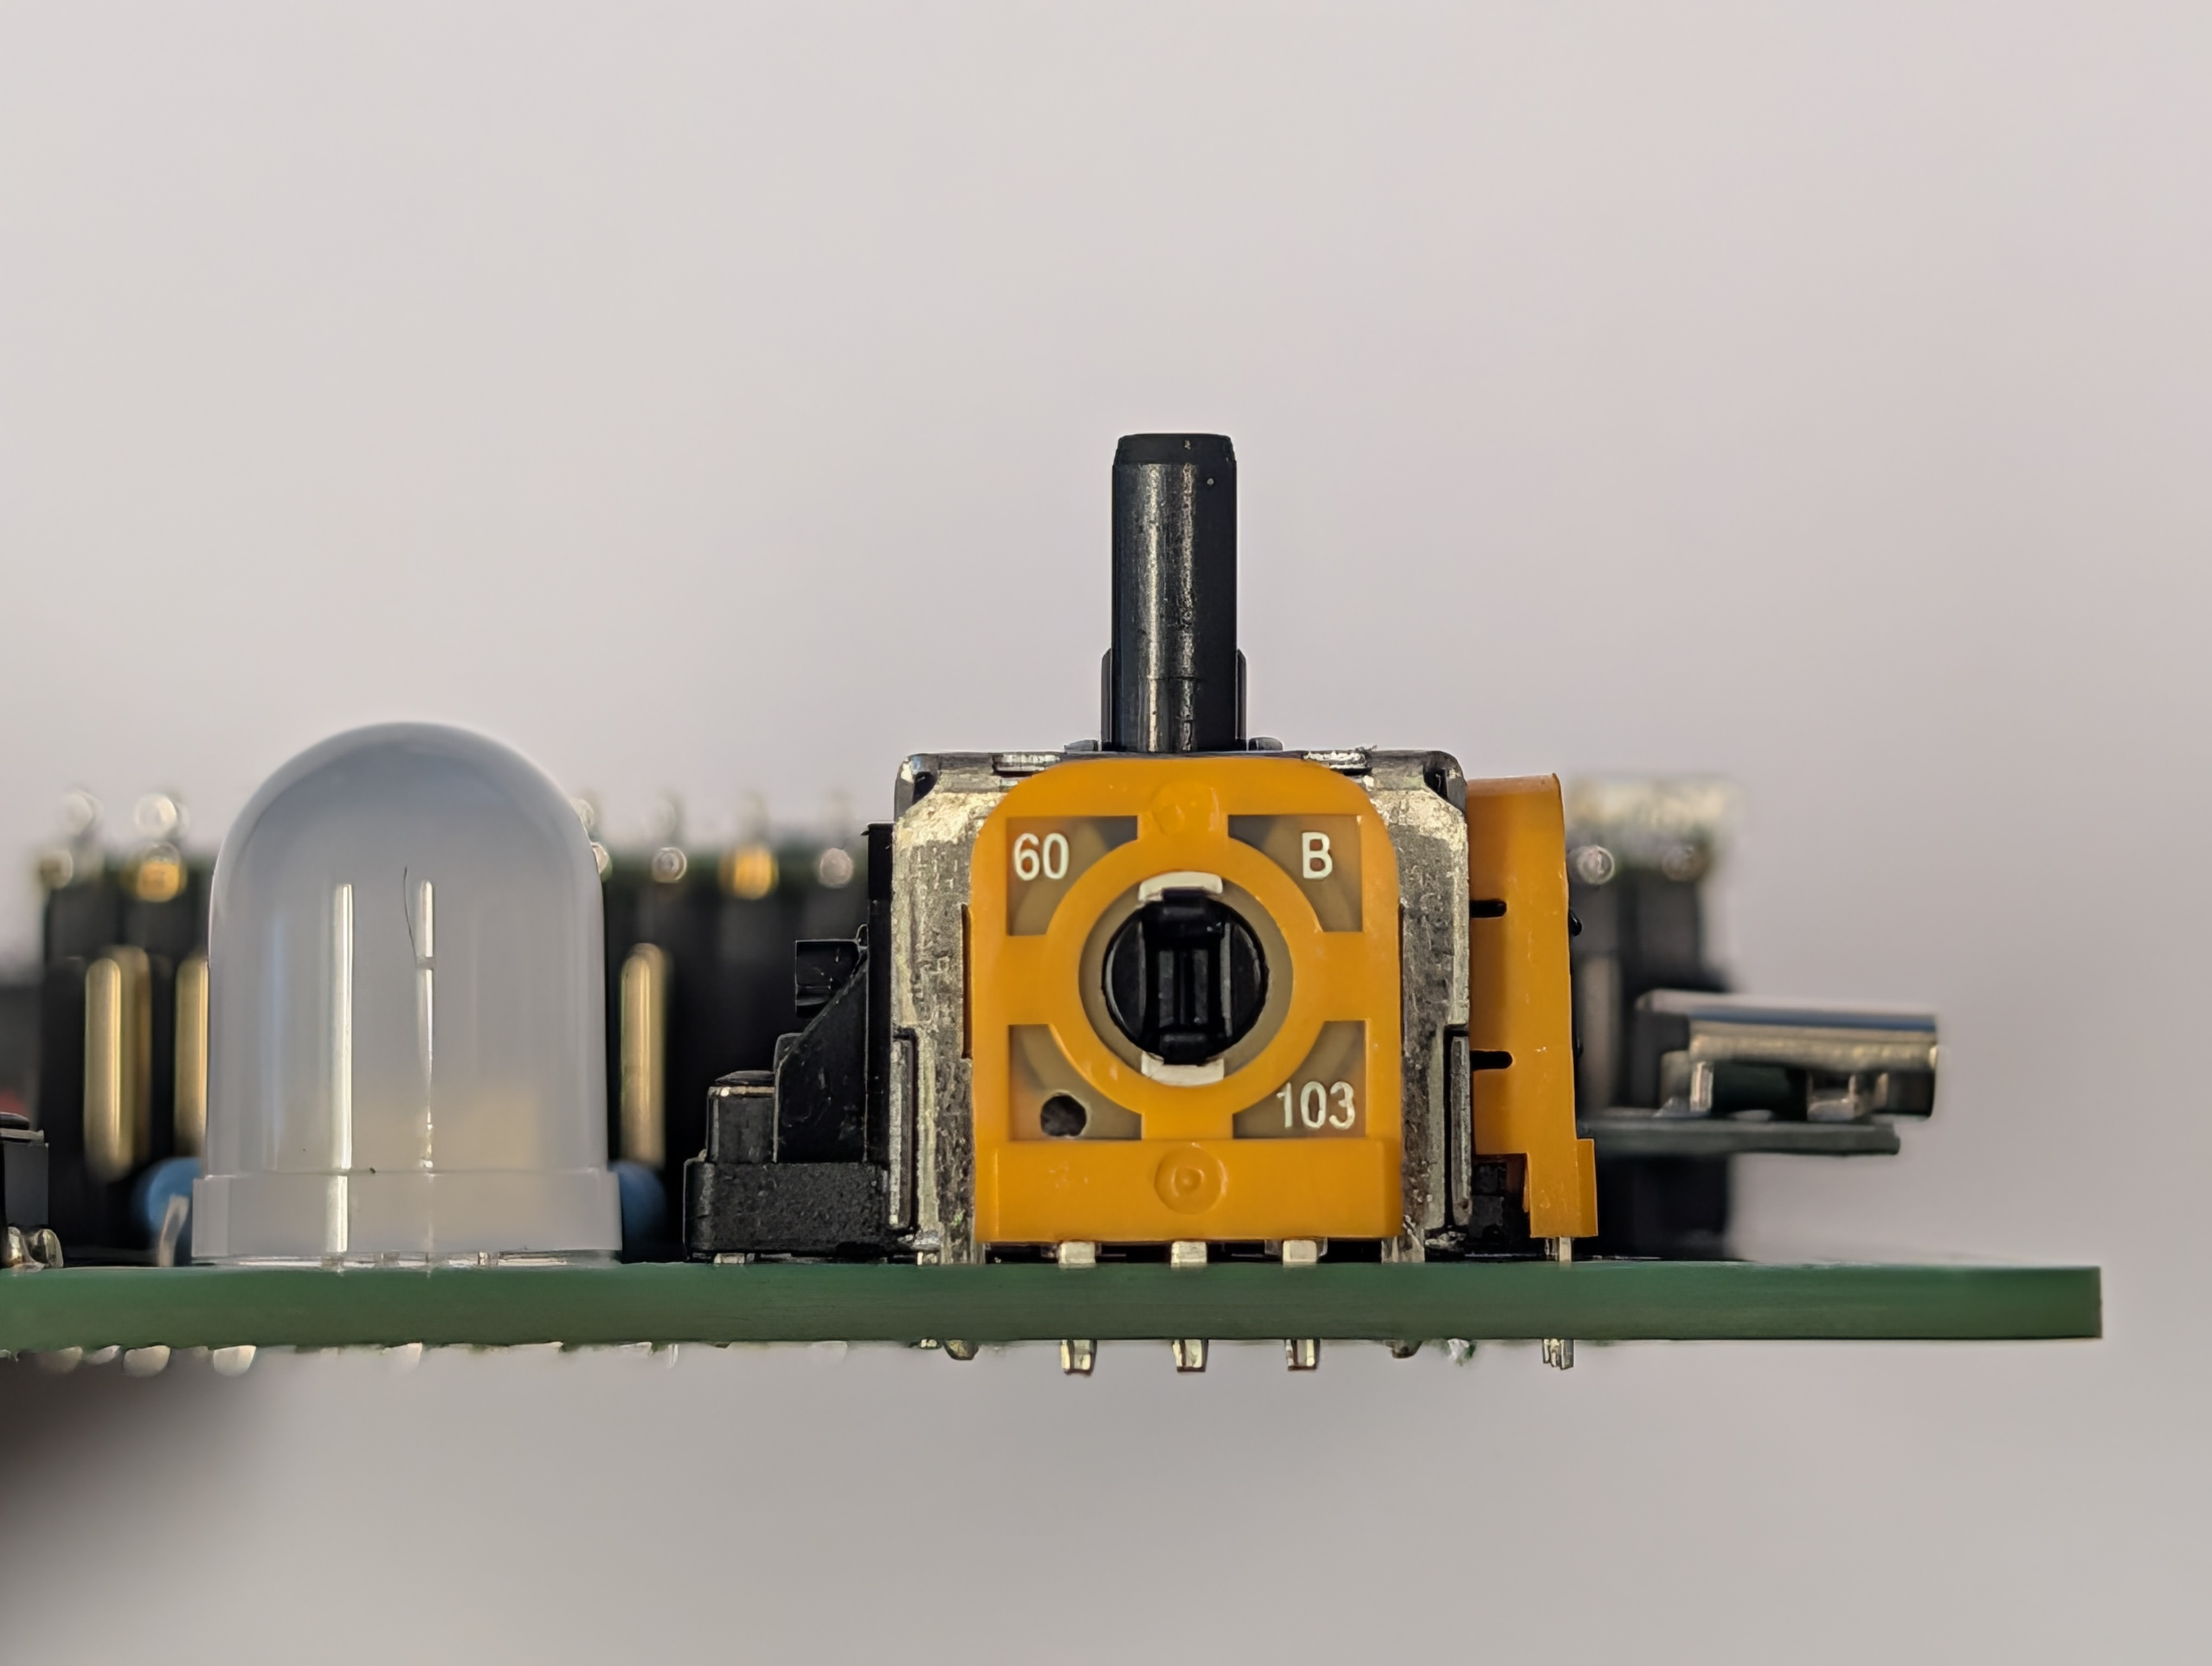
\includegraphics[width=0.75\textwidth]{pictures_of_construction/instruction_step_78.jpg}
\end{figure}

\begin{figure}[H]
    \centering
    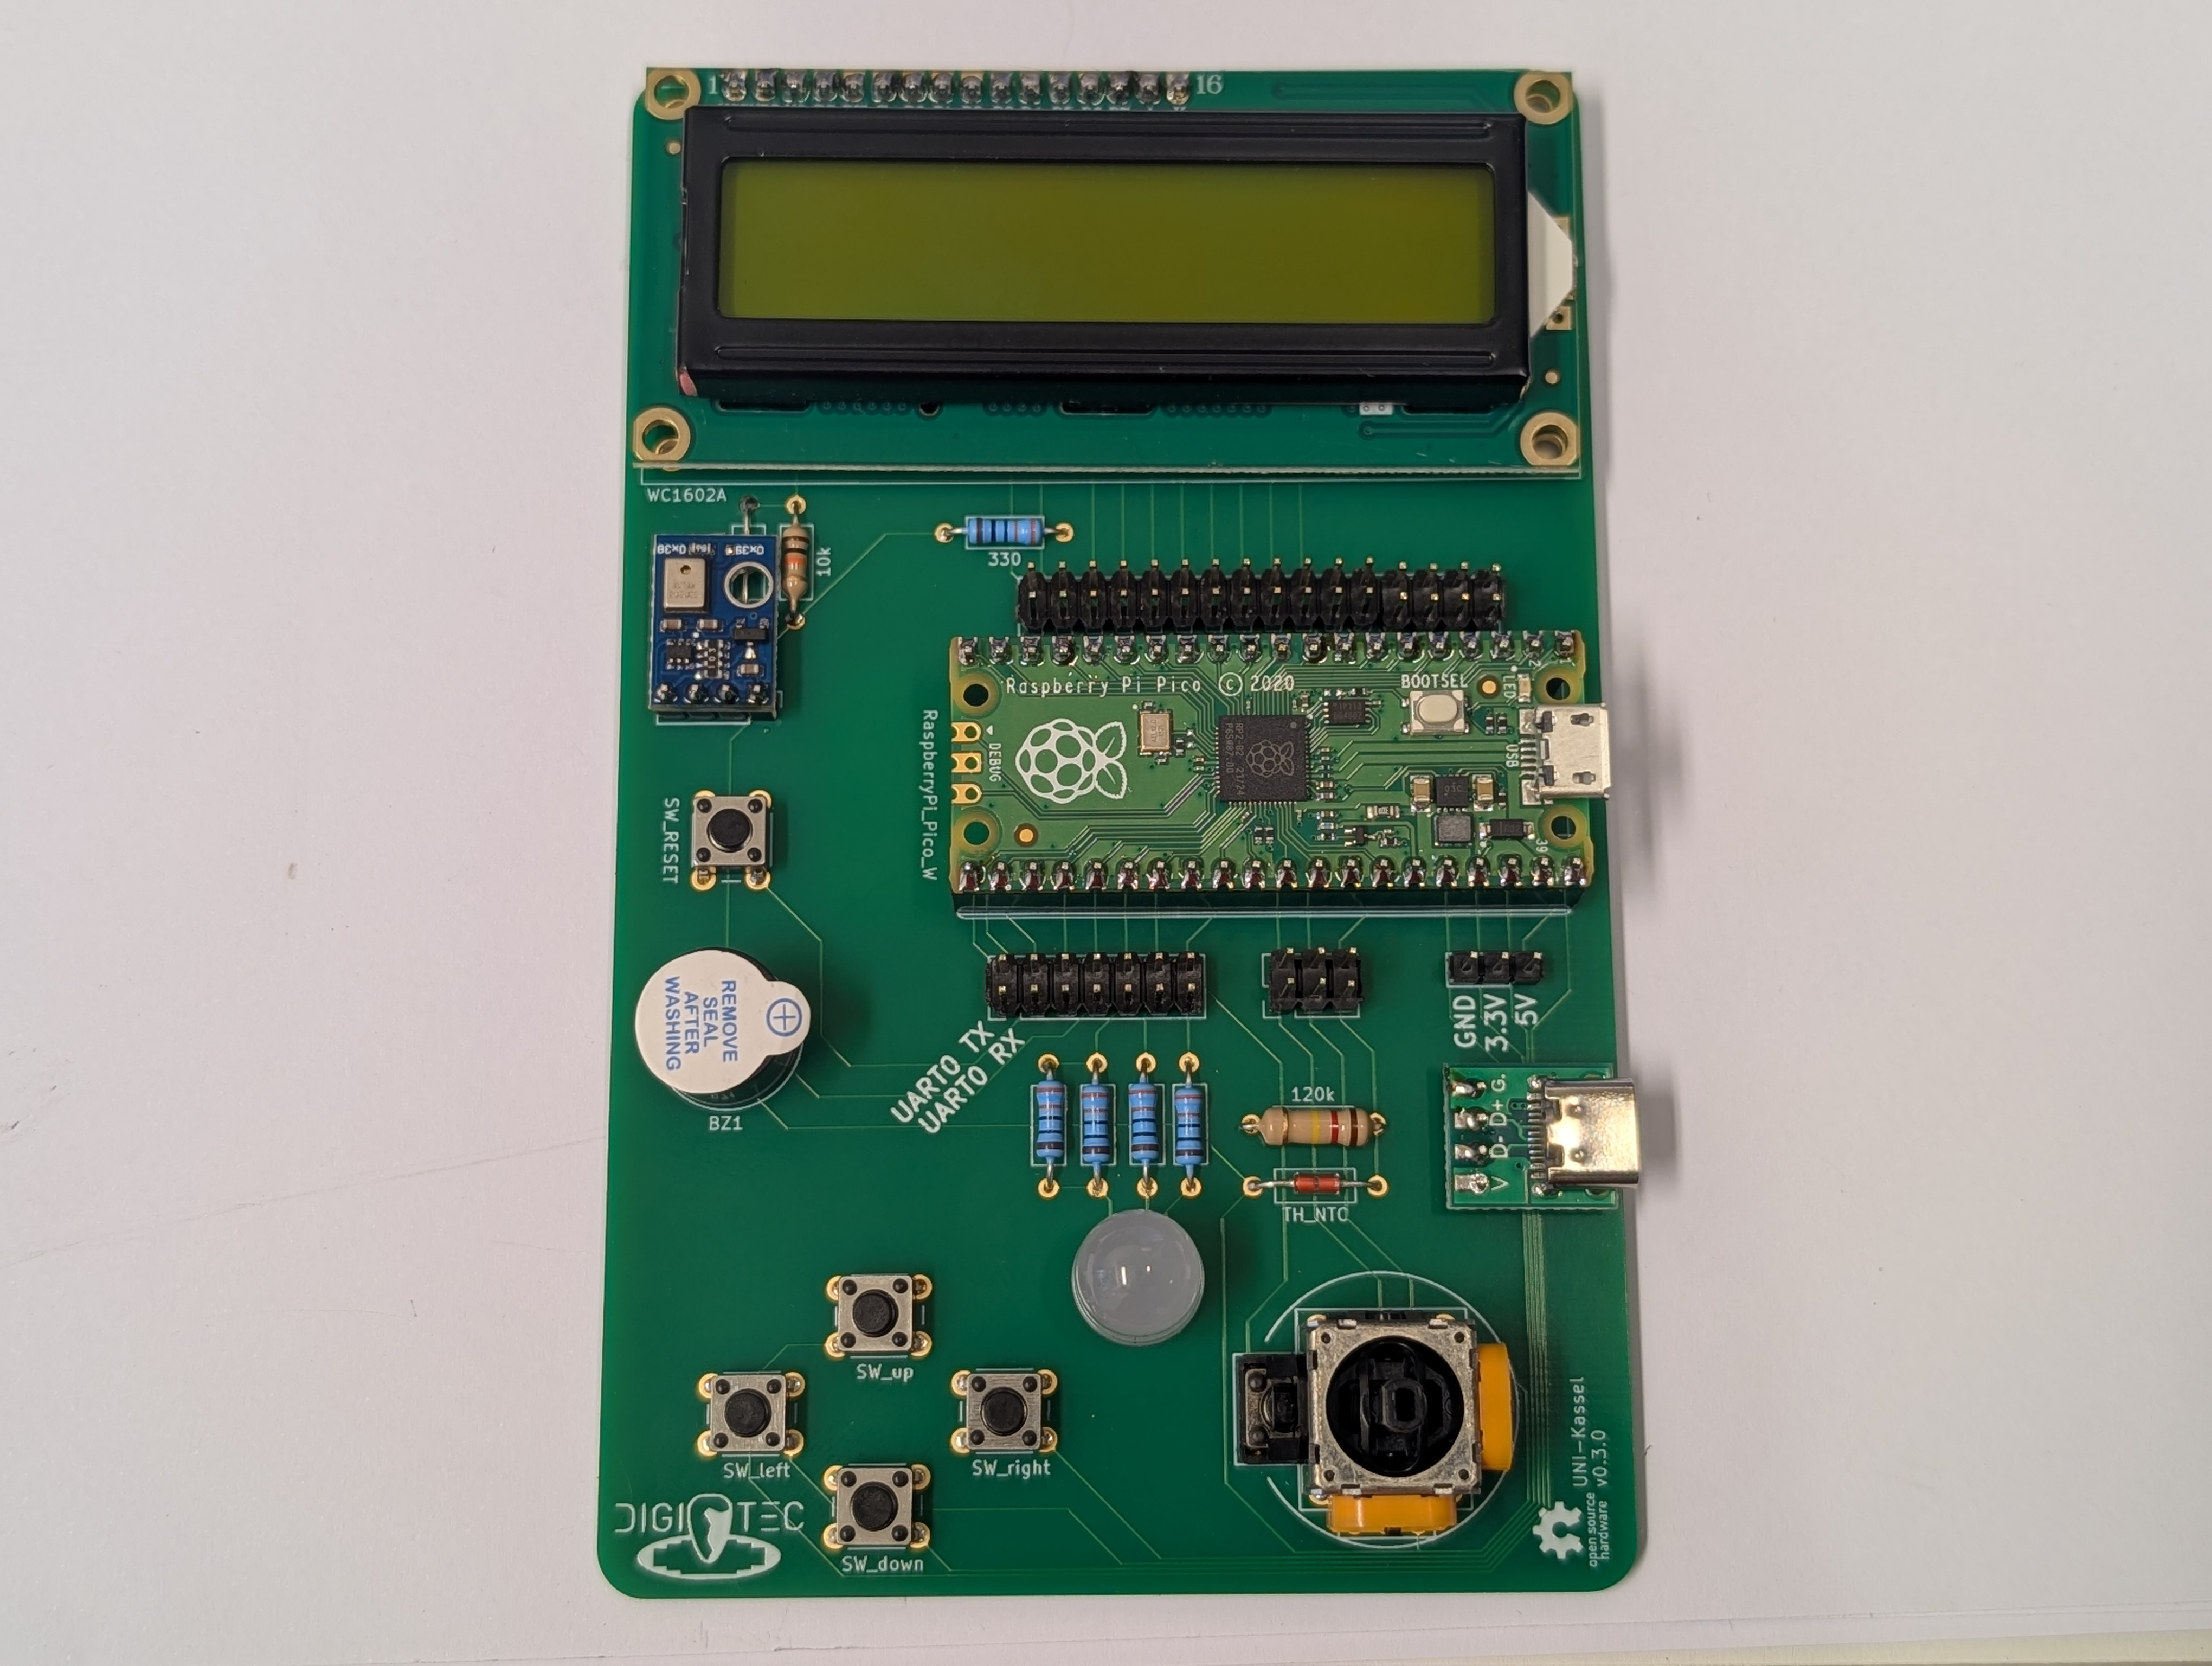
\includegraphics[width=0.75\textwidth]{pictures_of_construction/instruction_step_79.jpg}
\end{figure}

\subsection*{15. Jumper einsetzen}

Bevor du die Platine testen kannst, musst du noch alle \textbf{26 Jumper} einsetzen.

Stecke sie so auf wie in der Vorlage bzw. auf dem Bild in der Originalanleitung.

Erst danach ist die Platine vollständig bereit.

\begin{figure}[H]
    \centering
    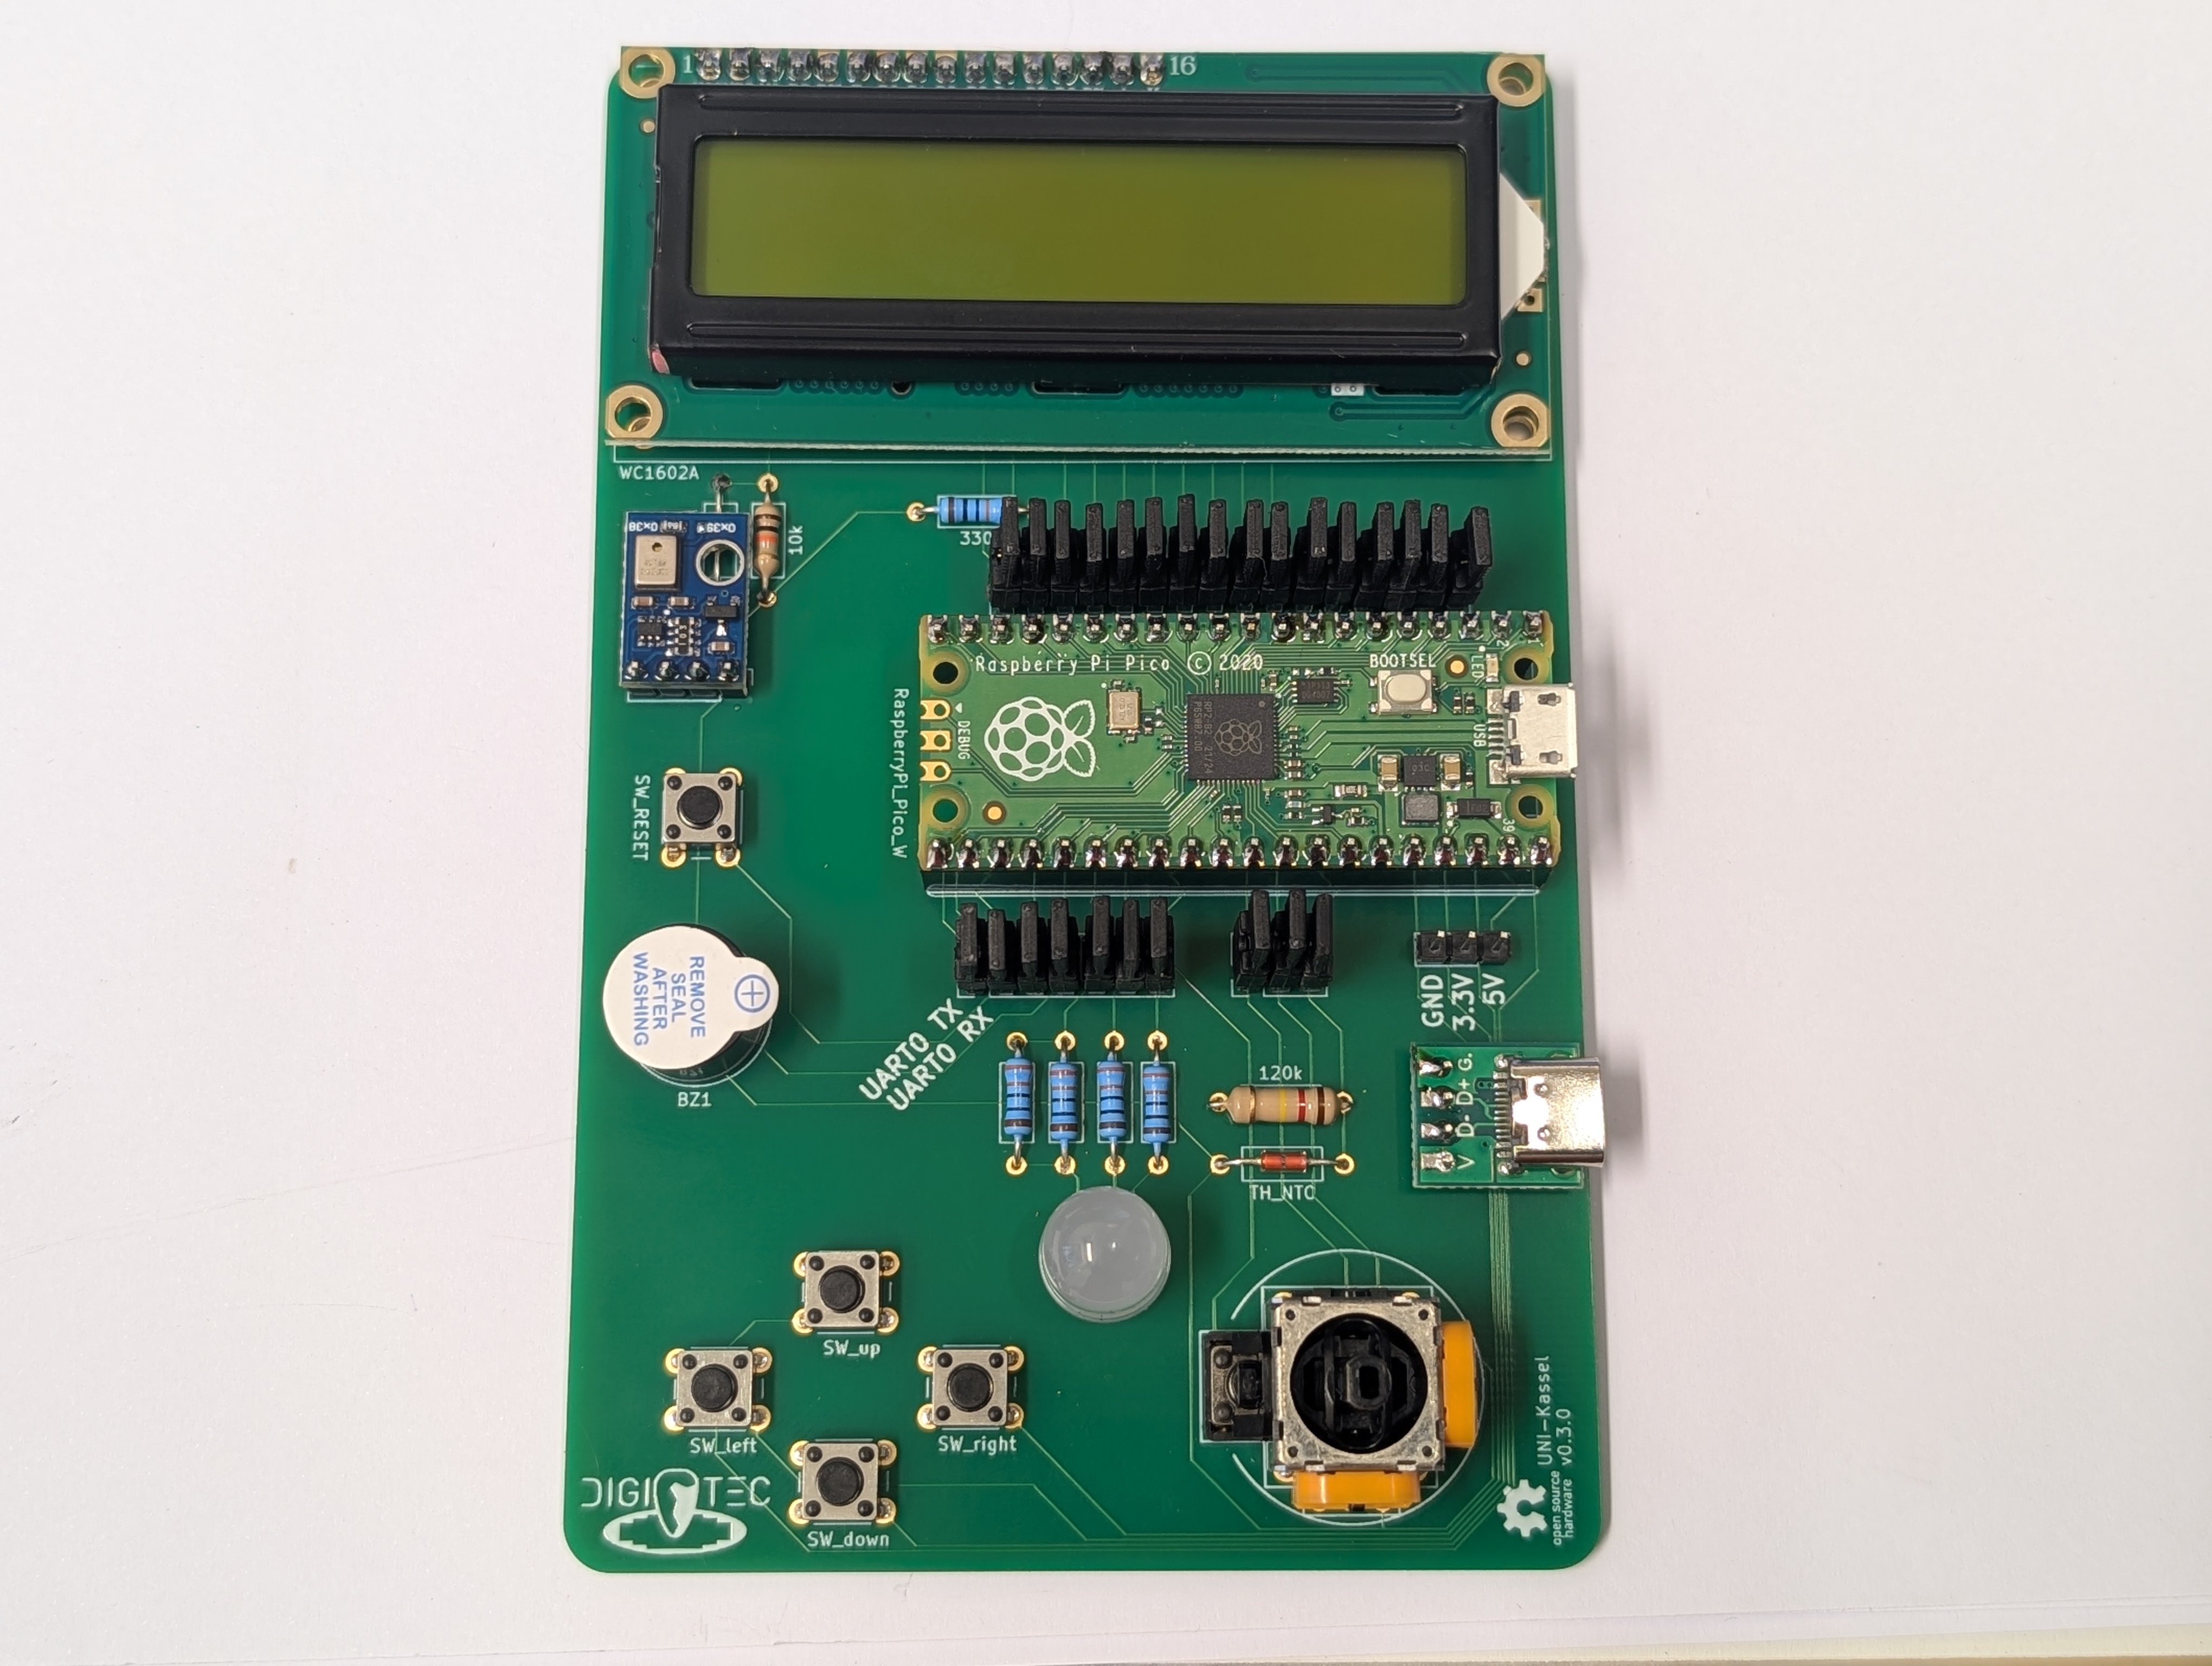
\includegraphics[width=0.75\textwidth]{pictures_of_construction/instruction_step_80.jpg}
\end{figure}

\section*{Geschafft!}

\textbf{Herzlichen Glückwunsch!}\\
Du hast den Buzzerino zusammengebaut.

\section*{Programm aufspielen}

Wenn auf dem Raspberry Pi Pico noch kein Programm ist, kannst du eine Datei wie \texttt{self\_test.uf2} darauf kopieren.

So geht’s:
\begin{enumerate}
    \item Halte die \textbf{BOOTSEL-Taste} auf dem Raspberry Pi Pico gedrückt.
    \item Verbinde den Pico mit einem USB-Kabel mit dem Computer.
    \item Am Computer erscheint ein Laufwerk mit dem Namen \textbf{RPI-RP2}.
    \item Ziehe die \texttt{.uf2}-Datei auf dieses Laufwerk.
    \item Danach startet der Pico automatisch neu.
\end{enumerate}

\section*{Noch ein paar einfache Tipps}

\begin{itemize}
    \item Löte lieber \textbf{langsam und sauber} als schnell.
    \item Wenn etwas schief sitzt: erst korrigieren, dann weiterlöten.
    \item Schneide Drahtenden immer erst ab, wenn alles richtig sitzt.
    \item Wenn du unsicher bist, frage nach Hilfe.
\end{itemize}

\end{document}